% -*- compile-command: "make HOCKING-slides.pdf" -*-
\documentclass{beamer}
\usepackage{tikz}
\usepackage[all]{xy}
\usepackage{amsmath,amssymb}
\usepackage{hyperref}
\usepackage{graphicx}
\usepackage{algorithmic}
\usepackage{multirow}

\DeclareMathOperator*{\argmin}{arg\,min}
\DeclareMathOperator*{\Lik}{Lik}
\DeclareMathOperator*{\Peaks}{Peaks}
\DeclareMathOperator*{\Segments}{Segments}
\DeclareMathOperator*{\argmax}{arg\,max}
\DeclareMathOperator*{\maximize}{maximize}
\DeclareMathOperator*{\minimize}{minimize}
\newcommand{\sign}{\operatorname{sign}}
\newcommand{\RR}{\mathbb R}
\newcommand{\ZZ}{\mathbb Z}
\newcommand{\NN}{\mathbb N}
\definecolor{pDPA}{HTML}{1B9E77}
\definecolor{PELT}{HTML}{D95F02}
\definecolor{FPOP}{HTML}{7570B3}
\newcommand{\algo}[1]{\textcolor{#1}{#1}}
\definecolor{PDPA}{HTML}{66C2A5}
\definecolor{CDPA}{HTML}{FC8D62}
\definecolor{GPDPA}{HTML}{4D4D4D}




% Set transparency of non-highlighted sections in the table of
% contents slide.
\setbeamertemplate{section in toc shaded}[default][100]
\AtBeginSection[]
{
  \setbeamercolor{section in toc}{fg=red} 
  \setbeamercolor{section in toc shaded}{fg=black} 
  \begin{frame}
    \tableofcontents[currentsection]
  \end{frame}
}

\begin{document}

\title{Statistical machine 
learning algorithms for 
understanding big data in
  genomics and medicine}

\author{
  Toby Dylan Hocking\\
  toby.hocking@mail.mcgill.ca
}

\maketitle

\begin{frame}
  \frametitle{Toby Dylan Hocking, brief CV}
  \begin{description}
  \item[2002-2006] UC Berkeley, double major in Molecular Cell Biology
    and Statistics (honors thesis with Terry Speed).
  \item[2006-2008] Biochemistry and Statistics at Sangamo BioSciences.
  \item[2008-2009] Masters in Statistics, Paris 6.
  \item[2009-2012] PhD in Mathematics from Ecole Normale Superieure de
    Cachan, machine learning for cancer genomics with JP Vert (Inst Curie)
    and Francis Bach (INRIA).
  \item[2013] Postdoc in Computer Science (machine learning) with Masashi Sugiyama at Tokyo
    Institute of Technology.
  \item[2014-2017] Postdoc on machine learning for epigenomics
    at McGill with Guillaume Bourque.
  \end{description}
\end{frame}

\section{Introduction to machine learning}

\begin{frame}
  \frametitle{Labeling enables supervised machine learning algorithms}
  \begin{tabular}{ccc}
    Input: Photos & Cell images & Copy number profiles \\
    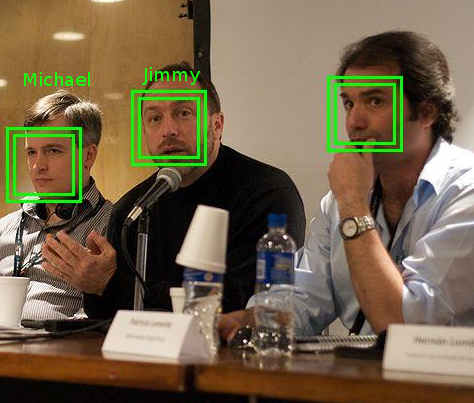
\includegraphics[width=1.3in]{faces} &
    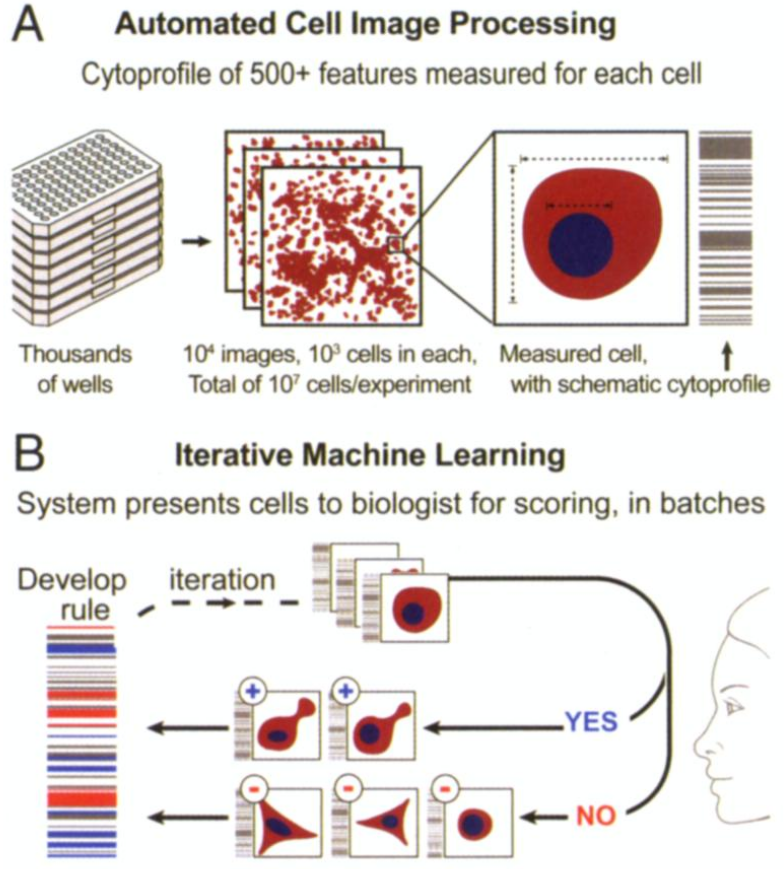
\includegraphics[width=1.3in]{cellprofiler} &
    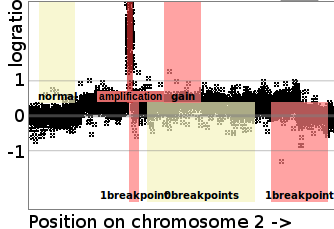
\includegraphics[width=1.5in]{regions-axes}\\
    Labels: boxes, names & phenotypes & alterations \\ \\
    %CVPR 2013
CVPR 2017
 & CellProfiler & SegAnnDB \\
    %246 papers
783 papers
 & 
%873 citations
1980 citations
 & H {\it et al.}, 2014. \\
     &
  \end{tabular}
  Sources: \url{http://en.wikipedia.org/wiki/Face_detection}\\
  Jones {\it et al.} PNAS 2009. Scoring diverse cellular morphologies in
  image-based screens with iterative feedback and machine learning.
\end{frame}

\begin{frame}
  \frametitle{Machine learning in computer vision and biology}
  ML is all about learning predictive functions $f(x)\approx y$, where 
  \begin{itemize}
  \item inputs/features $x$ are numerous (e.g. pixels or SNPs).
  \item outputs/labels $y$ are what we want to predict (typically
    phenotypes/classes).
  \item Input $x$ = image of digit,
    output $y\in\{0,1,\dots,9\}$,\\
  $f(
\includegraphics[height=1cm]{mnist-0})=0$,
  $f(
\includegraphics[height=1cm]{mnist-1})=1$
  % \item Input $x$ = image of article of clothing,\\
  %   output $y\in\{\text{shoe}, \text{pants}, \dots\}$,\\
  % $f(
\includegraphics[height=1cm]{fashion-mnist-boot})=\text{shoe}$,
  % $f(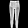
\includegraphics[height=1cm]{fashion-mnist-pants})=\text{pants}$
  \item Input $x$ = image of cell, 
    output $y\in\{\text{yes}, \text{no}\}$,\\
  $f(
\includegraphics[height=1cm]{cellprofiler-yes})=\text{yes}$,
  $f(
\includegraphics[height=1cm]{cellprofiler-no})=\text{no}$
  \item Input $x$ = genomic profile, output $y\in\{\text{breakpoint}, \text{normal}\}$
  $f(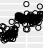
\includegraphics[height=1cm]{neuroblastoma-changepoint})=\text{breakpoint}$,
  $f(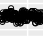
\includegraphics[height=1cm]{neuroblastoma-nochange})=\text{normal}$
  \end{itemize}
\end{frame}


\begin{frame}
  \frametitle{Supervised machine learning }

  \begin{itemize}
  \item Domain expert labels examples using prior knowledge.
  \item Supervised algorithm learns $f$ based on labeled training data.
  \item State-of-the-art accuracy (if there is enough training data).
  \item Can use same learning algorithm regardless of pattern.
  \end{itemize}

  \begin{tabular}{cc}
  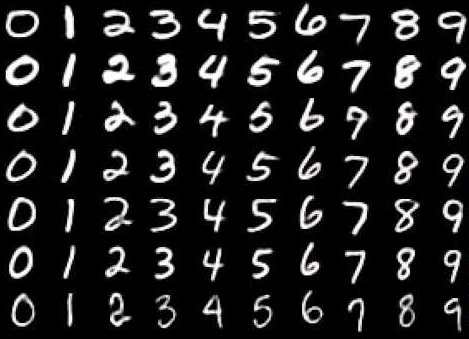
\includegraphics[height=1in]{mnist-digits} &
  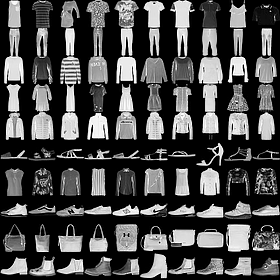
\includegraphics[height=1in]{fashion-mnist-sprite-some}  
  \end{tabular}

  \scriptsize Sources: github.com/cazala/mnist, github.com/zalandoresearch/fashion-mnist

  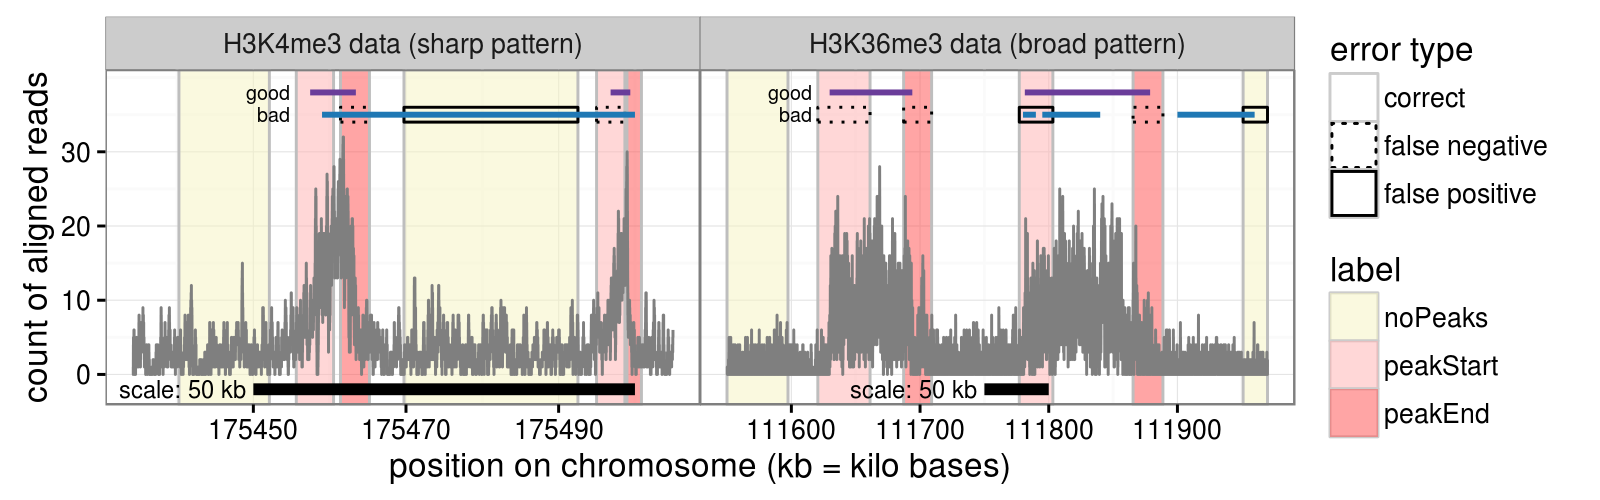
\includegraphics[width=\textwidth]{figure-good-bad}
\end{frame}

\begin{frame}
  \frametitle{My main research interests}
  Statistics and machine learning literature (methods development):
  \begin{itemize}
  \item Given features $x_i$, how to learn a function $f(x_i)$ that predicts a
    label $y_i$, with minimal error $E$ with respect to test data? 
    $$
\min_f
\sum_{i\in\text{test}}
E[f(x_i), y_i]
$$
\item Fast convex and discrete optimization algorithms that scale
  linearly to huge data sets -- important for genomics.
  %\item Convex and discrete optimization.
  \end{itemize}
  Bioinformatics and biomedical literature (applications):
  \begin{itemize}
  \item New labeling methods to facilitate collaborations between
    machine learners and genomic/medical scientists.
  \item Collaborations: applying machine learning methods to
    better understand biology/medicine.
  \end{itemize}
\end{frame}

\section{Predicting asthma and other autoimmune diseases based on
  genetic variants}

\begin{frame}
  \frametitle{Machine learning for predicting autoimmune disease based on genetic variants}
  \begin{itemize}
  \item Collaboration with Audrey Grant and Mark Lathrop.
  \item $n=120,286$ white UK citizens, aged 40-70.
  \item Genotyped using microarrays, 32 markers selected using
    univariate logistic regression test, 328 HLA alleles imputed.
  \item $x\in\{0,1,2\}^p$ = vector of allele counts and sex indicator.
  \item $f(x)\in\{0,1\}$ for predicting disease (1) or not (0).
  \item $f(x)=w^\intercal x + \beta$ L1-regularized logistic
    regression (glmnet R package), automatic feature selection.
  \item Scientific questions: which diseases can be predicted by
    genetics? Are both HLA and SNPs necessary? Are SNPs redundant?
  \item Main novelty: UK BioBank data set.
  \end{itemize}
\end{frame}

\begin{frame}
  \frametitle{Both HLA and markers selected in L1 regularized logistic regression
    model for predicting asthma }

  \begin{minipage}{0.39\linewidth}
    \begin{itemize}
    \item Right: many unused HLA alleles in the predictive model, one
      unused SNP.
    \item Below: SNP markers more accurate than HLA alleles.
    \end{itemize}
  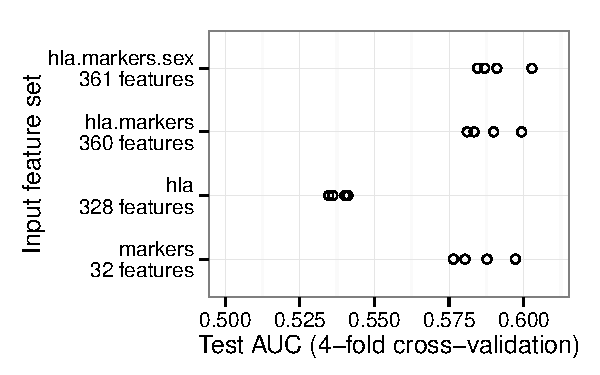
\includegraphics[width=\textwidth]{figure-asthma-old}
  \end{minipage}
  \begin{minipage}{0.59\linewidth}
    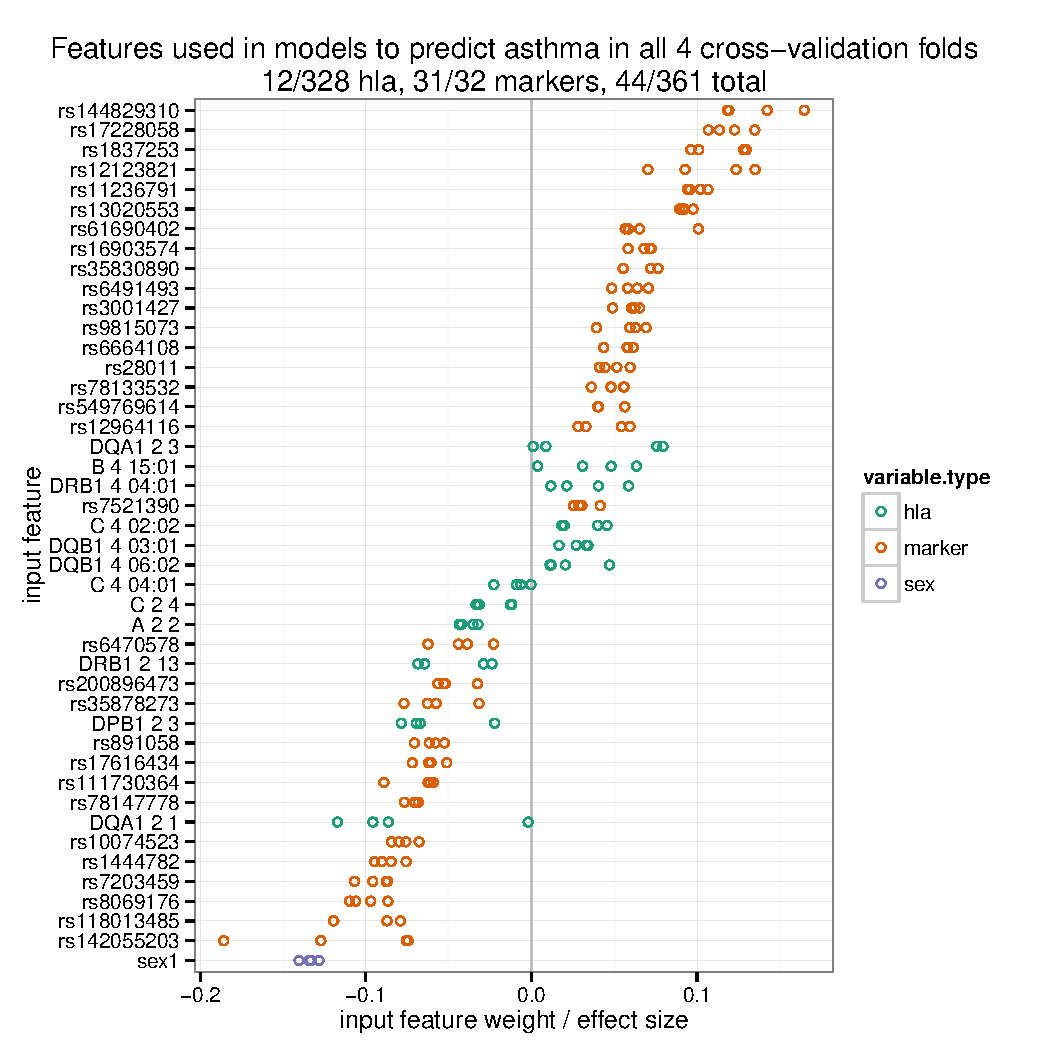
\includegraphics[width=\textwidth]{figure-asthma-4folds}
  \end{minipage}
\end{frame}
 
\begin{frame}
  \frametitle{L1-regularized logistic regression model automatically selects relevant HLA features for each
    disease}

  \begin{itemize}
  \item HLA features predict some diseases more accurately than others.
  \item Different number of features selected per disease.
  \end{itemize}
  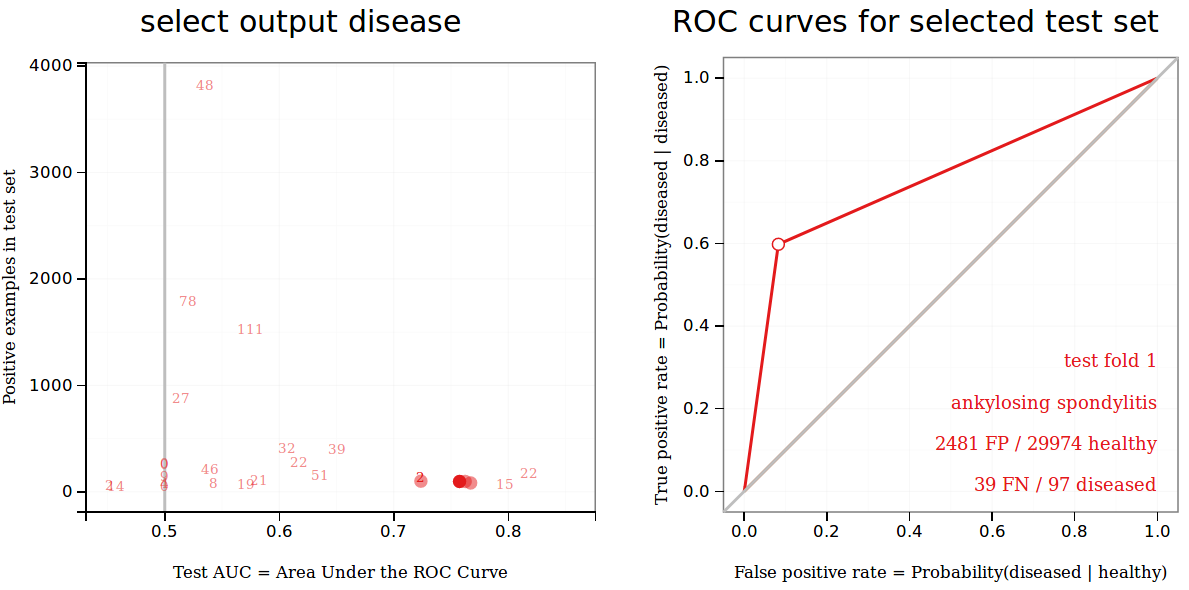
\includegraphics[width=\textwidth]{screenshot-ankylosing-spondylitis}

\scriptsize  \url{http://members.cbio.ensmp.fr/~thocking/figure-asthma-test-error/}
\end{frame}

\section{Learning a predictive pathogenicitity score for genetic variants}

\begin{frame}
  \frametitle{Machine learning setup for variant prioritization}
  \begin{itemize}
  \item $x\in\mathbb R^p$ = vector of scores from 
    annotation programs (evolutionary conservation, biochemical
    modeling, etc).
  \item $f(x)\in\{0,1\}$ for predicting whether the variant is
    pathogenic (1) or benign (0).
  \item Existing methods to learn $f$: L1-regularized logistic
    regression, random forests, boosting.
  \item Scientific question: is the learned score more accurate than
    the individual scores? Which features are relevant for predicting
    pathogenicity?
  \item Main novelty: train on ClinVar data set 2013--2015
    (common/rare missense variants, 7059 benign, 4023 pathogenic)
  \end{itemize}
\end{frame}


\begin{frame}
  \frametitle{Learned scores predict pathogenicity more accurately}
  \begin{itemize}
  \item Learned ClinPred scores more accurately predict
    Pathogenic/Benign status in held-out test sets (ClinVar 2016,
    four-fold cross-validation).
  \item AF=Allele Frequency feature essential for optimal accuracy.
  \item All features selected in L1-regularized logistic regression.
  \end{itemize}
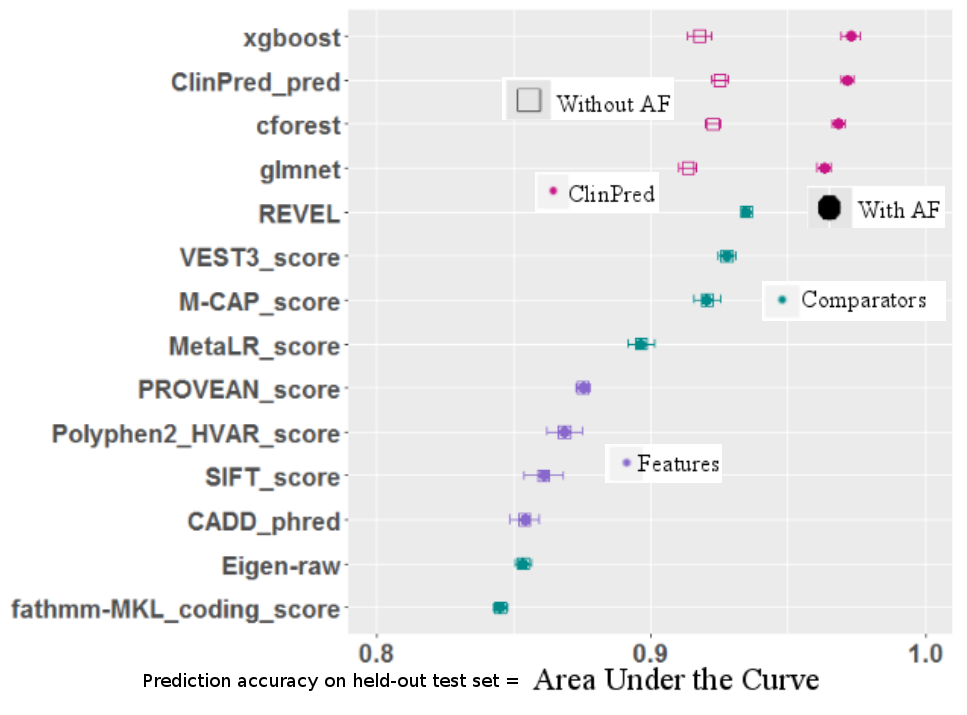
\includegraphics[width=0.7\textwidth]{Screenshot-clinpred-auc}
\end{frame}

\begin{frame}
  \frametitle{Learned scores predict accurately for variants in mouse}
  But so does allele frequency (ExAC\_ALL).
  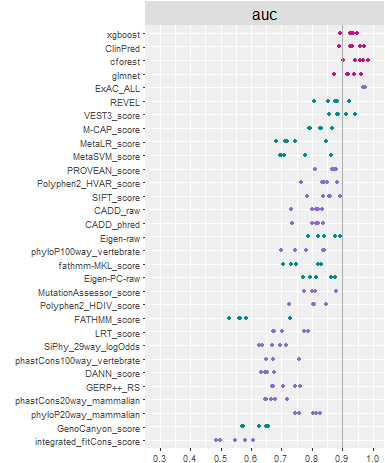
\includegraphics[width=0.6\textwidth]{variants-auc-mouse}
\end{frame}
 
\section{Predicting breakpoint positions in DNA copy number profiles}

\begin{frame}
  \frametitle{Cancer cells show chromosomal copy number alterations}
  Spectral karyotypes show the number of copies of the sex chromosomes
  (X,Y) and autosomes (1-22). 

  Source: Alberts \emph{et al.} 2002.
\vskip 0.1in
  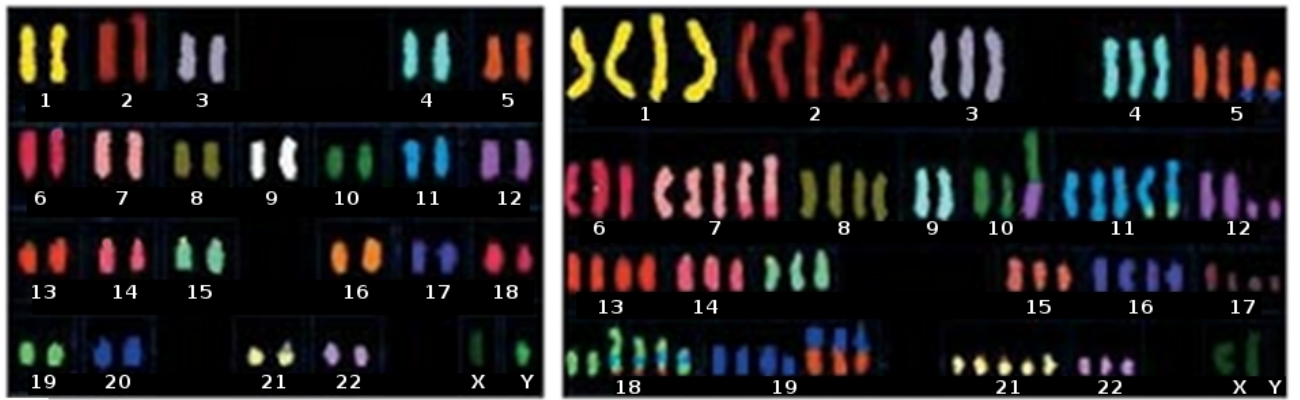
\includegraphics[width=\textwidth]{Karyo-both}
\vskip 0.1in
  \begin{minipage}{0.4\linewidth}
    Normal cell with 2 copies of each autosome.
  \end{minipage}
\hskip 0.1\linewidth
  \begin{minipage}{0.4\linewidth}
Cancer cell with many copy number alterations.
  \end{minipage}
\end{frame}

\begin{frame}
  \frametitle{Breakpoint detection is important in cancers such as
    neuroblastoma } 

  \begin{itemize}
  \item Childhood cancer, most frequently diagnosed at age 1--2.
  \item Top three profiles ``ok'' -- no tumors after initial treatment.
  \item Bottom three ``relapse'' -- aggressive tumor within 5 years.
  \item Previous work: relapse profiles tend to have more breakpoints
     (Schleiermacher {\it et al.}, 2010).
  \end{itemize}

  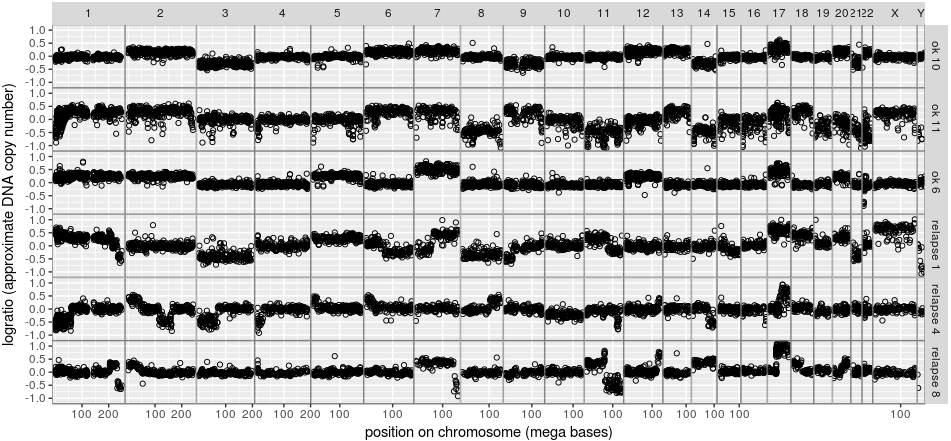
\includegraphics[width=\textwidth]{neuroblastoma-ok-relapse}
\end{frame}

\begin{frame}
  \frametitle{Breakpoint detection as a machine learning problem}
  
  \begin{itemize}
  \item Input $x\in\mathbb R^p$ = noisy copy number signal for $p$
    probes in one genome subset (chromosome).
  \item Typical data set sizes $10^2 < p < 10^5$ for microarrays.
  \item Structured binary classification problem: want to learn
    $f(x)\in\{0,1\}^{p-1}$ to predict a 
    \textcolor{green}{breakpoint} (1) or not (0).
    %after every data point (green lines).
  \item Previous algorithms: unsupervised learning (no labels).
  \end{itemize}

  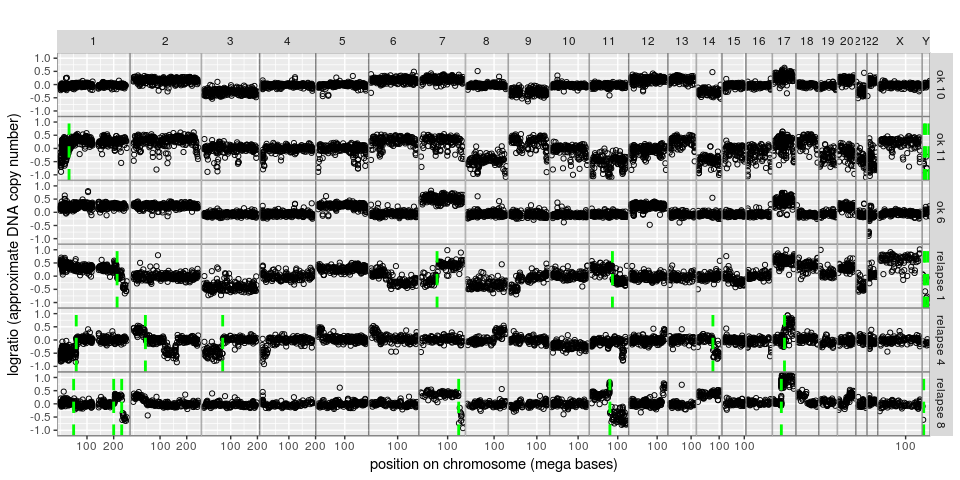
\includegraphics[width=\textwidth]{neuroblastoma-ok-relapse-pred}
\end{frame}

\begin{frame}
  \frametitle{New labeling and training methods for breakpoint detection}

  H {\it et al.}, {\it BMC Bioinformatics} 2013.
  \begin{itemize}
  \item Create positive/breakpoint and negative/normal labels.
  \item Quantify/optimize error rate (number of incorrect labels).
  \item Benchmark data set of 3418 chromosomes,
    labeled via visual inspection (R package neuroblastoma).
  \item Results: most accurate model is maximum Gaussian likelihood 
    changepoint detection (K-fold cross-validation experiments).
  \end{itemize}

  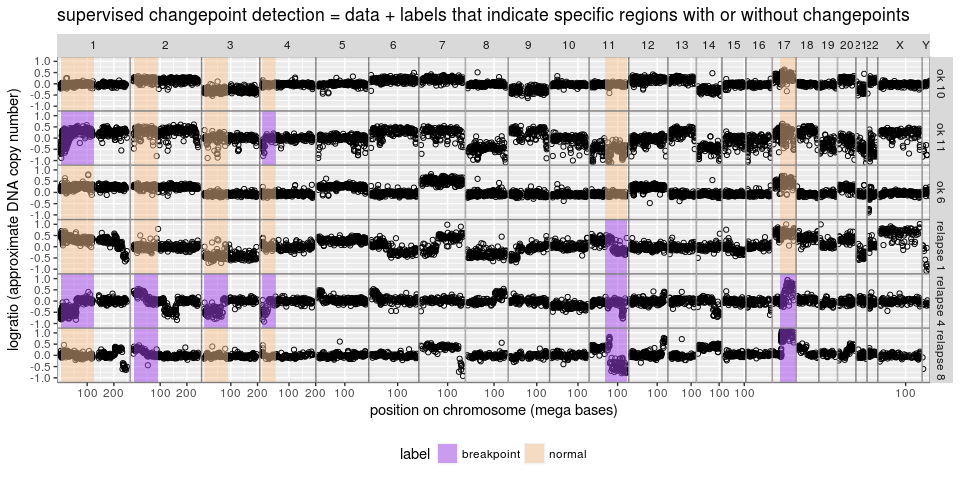
\includegraphics[width=\textwidth]{neuroblastoma-ok-relapse-supervised}

\end{frame}

\begin{frame}
  \frametitle{Log-linear $O(p \log p)$ FPOP algorithm for computing one
    maximum
    likelihood changepoint model}

  Maidstone, Hocking, Rigaill, Fearnhead, {\it Stat. and
    Comp.} 2017.

  \begin{itemize}
  \item Naively $O(p^K)$ time to compute best model with $K$ segments
    ($K-1$ changes) for a sequence of $p$ data.
  \item Previous work: inequality pruning for computing 1 model (\algo{PELT}),
    functional pruning for computing $K$ models (\algo{pDPA}).
  \item Contribution: two new algorithms, SNIP and
    \algo{FPOP} (R package fpop).
  \item Proved that the functional technique prunes at least as many
    changepoints as the inequality technique (so is faster).
  \end{itemize}

  \begin{minipage}{0.55\linewidth}
        \begin{tabular}{c|cc}
      & \multicolumn{2}{c}{Pruning Technique}\\
*=new      & Functional & Inequality \\ 
\hline
      $K$ models & \algo{pDPA} & SNIP* \\
      1 model & \algo{FPOP}* & \algo{PELT}
    \end{tabular}
  \end{minipage}
  \begin{minipage}{0.4\linewidth}
    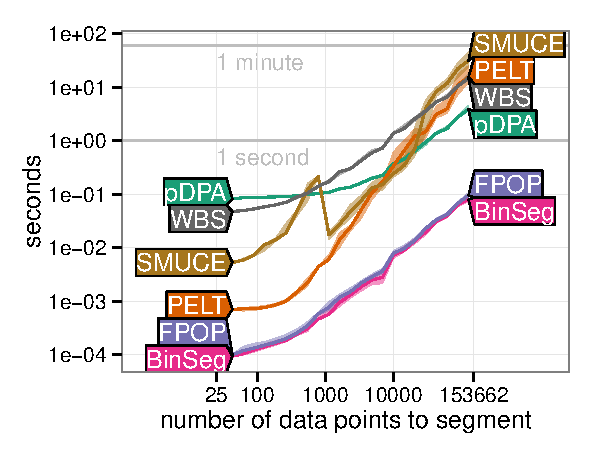
\includegraphics[width=\textwidth]{figure-systemtime-arrays-bins}
  \end{minipage}
\end{frame}

\begin{frame}
  \frametitle{Supervised interactive DNA copy number analysis}
  H {\it et al.}, {\it Bioinformatics} 2014.

  \begin{itemize}
  \item Previous work: non-interactive command line programs
    -- collaborators can not correct obvious
    errors.
  \item Interactive system: when you edit the labels, the system
    learns and updates the model. (SegAnnDB python module)
  \item Regression model for predicting the number of segments $K$ (H
    {\it et al.}, {\it ICML} 2013).
  \item Result: only a few labels required to learn a highly accurate
    breakpoint detection model.
  \end{itemize}
  \begin{minipage}{0.5\linewidth}
    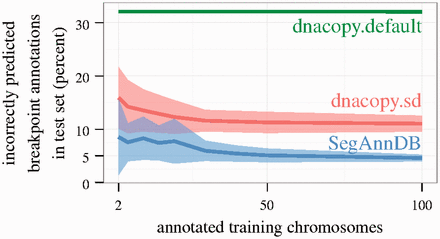
\includegraphics[width=\textwidth]{SegAnnDB-test-error-decreases}
  \end{minipage}
  \begin{minipage}[0.5\linewidth]{0.48\linewidth}
SegAnnDB demo:\\interactively label chr1 and chrX
  \url{http://bioviz.rocq.inria.fr/profile/GSM313887/}
  \end{minipage}
\end{frame}

\begin{frame}
  \frametitle{Cancer biology collaborations}
  Aichi cancer center, Nagoya, Japan.
  \begin{itemize}
  \item Suguro {\it et al.}, {\it Cancer Sci} 2014, Clonal
    heterogeneity of lymphoid malignancies correlates with poor
    prognosis.
  \item Shimada {\it et al.}, {\it Leukemia} 2016, Development and
    analysis of patient-derived xenograft mouse models in
    intravascular large B-cell lymphoma.
  \end{itemize}
  Institut Curie, Paris, France.
  \begin{itemize}
  \item Chicard {\it et al.}, {\it Clinical Cancer Research} 2016,
    Genomic copy number profiling using circulating free tumor DNA
    highlights heterogeneity in neuroblastoma.
  \item Ongoing work, characterizing alterations in neuroblastoma.
  \end{itemize}
\end{frame}

\section{Predicting peaks in ChIP-seq data}

\begin{frame}
  \frametitle{Chromatin immunoprecipitation sequencing (ChIP-seq)}
  Analysis of DNA-protein interactions: which genomic regions have
  bound/modified proteins?

  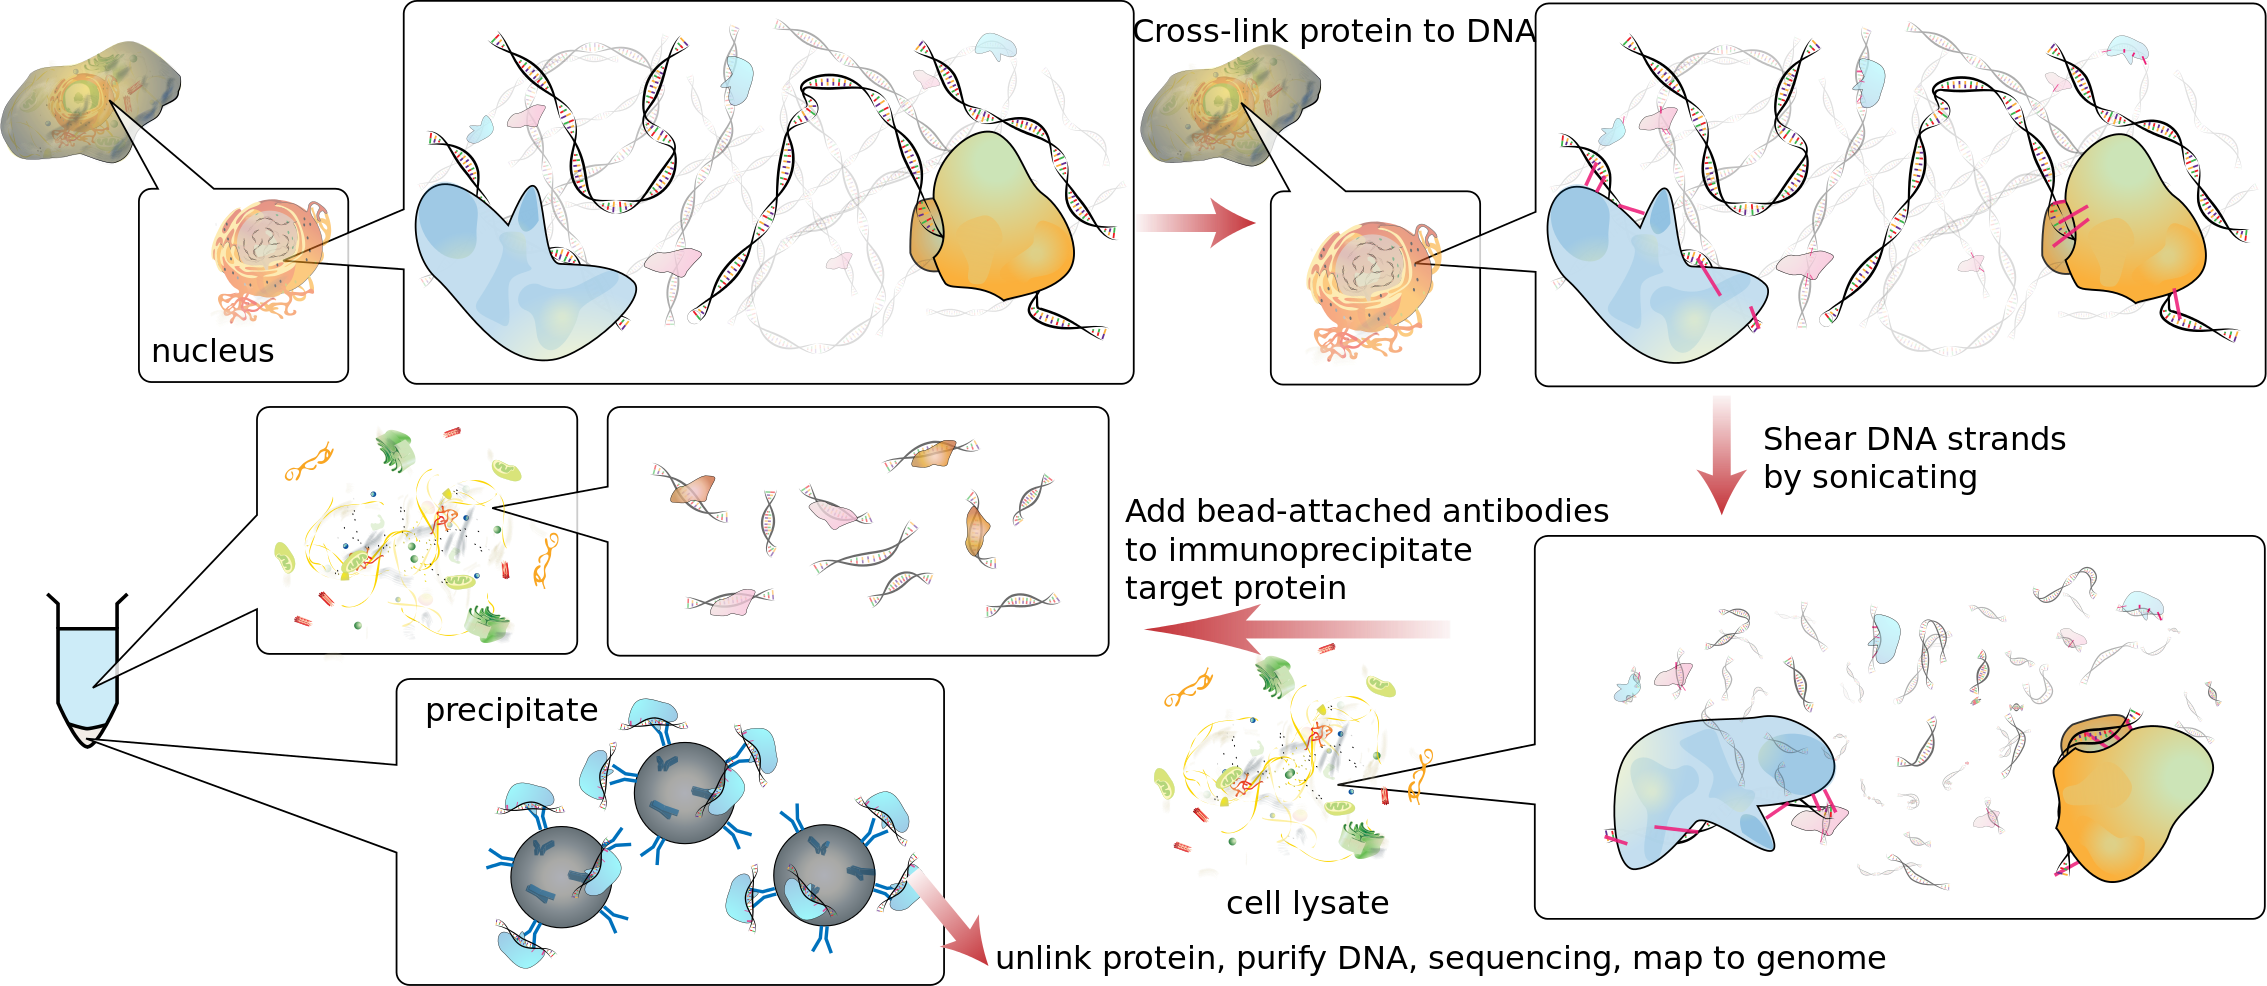
\includegraphics[width=\textwidth]{Chromatin_immunoprecipitation_sequencing_wide.png}

  Source: ``ChIP-sequencing,'' Wikipedia.
\end{frame}

% \begin{frame}
%   \frametitle{Problem: inaccurate unsupervised peak predictions}
%   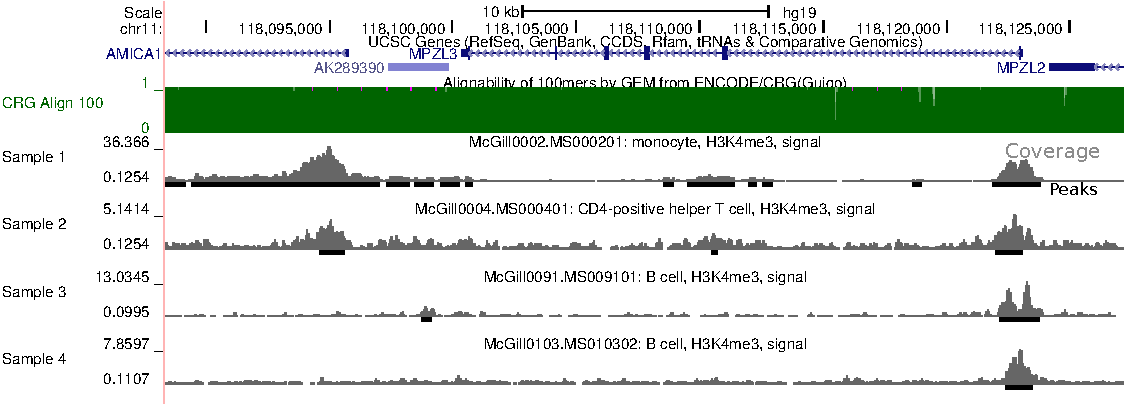
\includegraphics[width=\textwidth]{screenshot-ucsc-edited}

%   Grey profiles are normalized aligned read count signals.

%   Black bars are ``peaks'' called by MACS2 (Zhang {\it et al.}, 2008):
%   \begin{itemize}
%   \item many false positives (sometimes false negatives as well).
%   \item overlapping peaks have different start/end positions.
%   \end{itemize}
% \end{frame}

\begin{frame}
  \frametitle{Peak detection as a machine learning problem}
  
  \begin{itemize}
  \item Input $x\in\mathbb Z_+^n$ = noisy coverage profile for $n$ bases
    in a chromosome subset between gaps in reference genome.
  \item Typical data set sizes $10^5 < n < 10^8$ for ChIP-seq.
  \item Structured binary classification problem: want to learn
    $f(x)\in\{0,1\}^{n}$ to predict a  
    peak (1) or not (0).
  \item Previous algorithms: unsupervised learning (no labels).
  \end{itemize}
 
  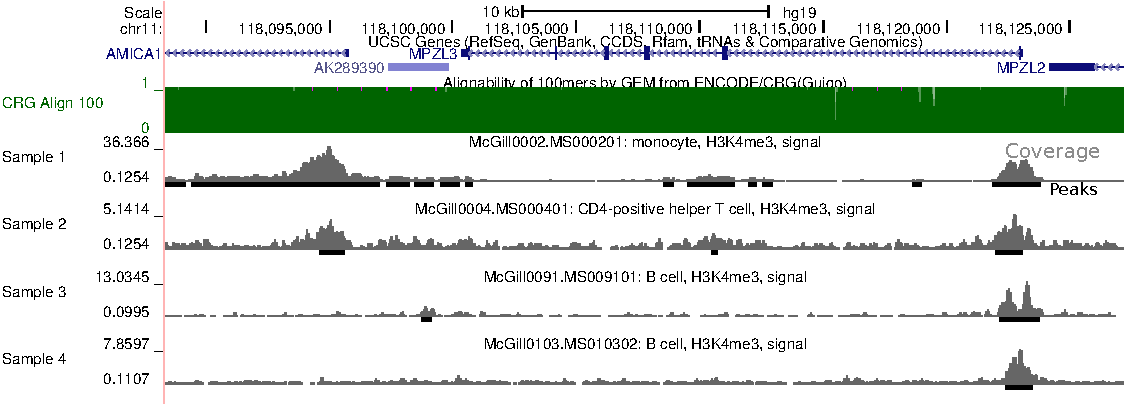
\includegraphics[width=\textwidth]{screenshot-ucsc-edited}
\end{frame} 

% \begin{frame}
%   \frametitle{Previous work in genomic peak detection}
%   \begin{itemize}
%   \item Model-based analysis of ChIP-Seq (MACS), Zhang et al, 2008.
%   \item SICER, Zang et al, 2009.
%   \item HOMER, Heinz et al, 2010.
%   \item CCAT, Xu et al, 2010.
%   \item RSEG, Song et al, 2011.
%   \item Triform, Kornacker et al, 2012.
%   \item Histone modifications in cancer (HMCan), Ashoor et al, 2013.
%   \item PeakSeg, Hocking, Rigaill, Bourque, ICML 2015.
%   \item PeakSegJoint Hocking and Bourque, arXiv:1506.01286.
%   \item ... dozens of others.
%   \end{itemize}
%   Two big questions: how to choose the best...
%   \begin{itemize}
%   \item ...algorithm? (testing)
%   \item ...parameters? (training)
%   \end{itemize}
% \end{frame}

% \begin{frame}[fragile]
%   \frametitle{How to choose parameters of unsupervised peak
%     detectors?}
% \scriptsize
% 19 parameters for Model-based analysis of ChIP-Seq (MACS), Zhang {\it et al.}, 2008.
% \begin{verbatim}
%   [-g GSIZE]
%   [-s TSIZE] [--bw BW] [-m MFOLD MFOLD] [--fix-bimodal]
%   [--nomodel] [--extsize EXTSIZE | --shiftsize SHIFTSIZE]
%   [-q QVALUE | -p PVALUE | -F FOLDENRICHMENT] [--to-large]
%   [--down-sample] [--seed SEED] [--nolambda]
%   [--slocal SMALLLOCAL] [--llocal LARGELOCAL]
%   [--shift-control] [--half-ext] [--broad]
%   [--broad-cutoff BROADCUTOFF] [--call-summits]
% \end{verbatim}
% 10 parameters for Histone modifications in cancer (HMCan),
% Ashoor {\it et al.}, 2013.
% \begin{verbatim}
% minLength 145
% medLength 150
% maxLength 155
% smallBinLength 50
% largeBinLength 100000
% pvalueThreshold 0.01
% mergeDistance 200
% iterationThreshold 5
% finalThreshold 0
% maxIter 20
% \end{verbatim}
% \end{frame}


\begin{frame}
  \frametitle{New labeling method for peak detection in ChIP-seq data}

  H {\it et al.}, {\it Bioinformatics} 2017: choose peak model/parameters
  which minimize the number of incorrectly predicted labels.

  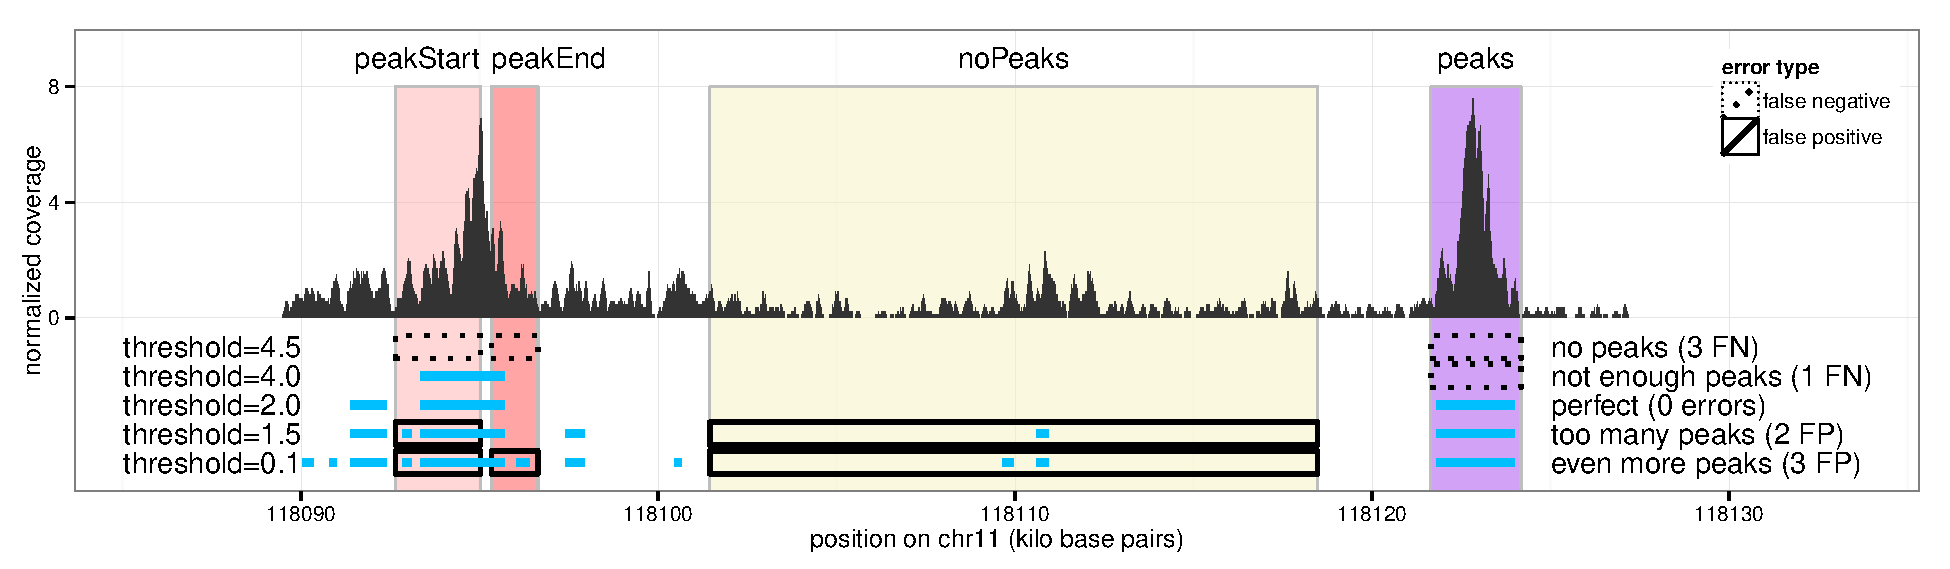
\includegraphics[width=\textwidth]{figure-PeakError.pdf}
  \begin{itemize}
  \item \textbf{peakStart}: exactly one peak start (0=FN, more=FP).
  \item \textbf{peakEnd}: exactly one peak end (0=FN, more=FP).
  \item \textbf{noPeaks}: no overlapping peaks (otherwise FP).
  \item \textbf{peaks}: at least one overlapping peak (otherwise FN).
  \item R package PeakError.
  \end{itemize}
\end{frame}

\begin{frame}
  \frametitle{Two annotators provide consistent labels, but different
    precision}
  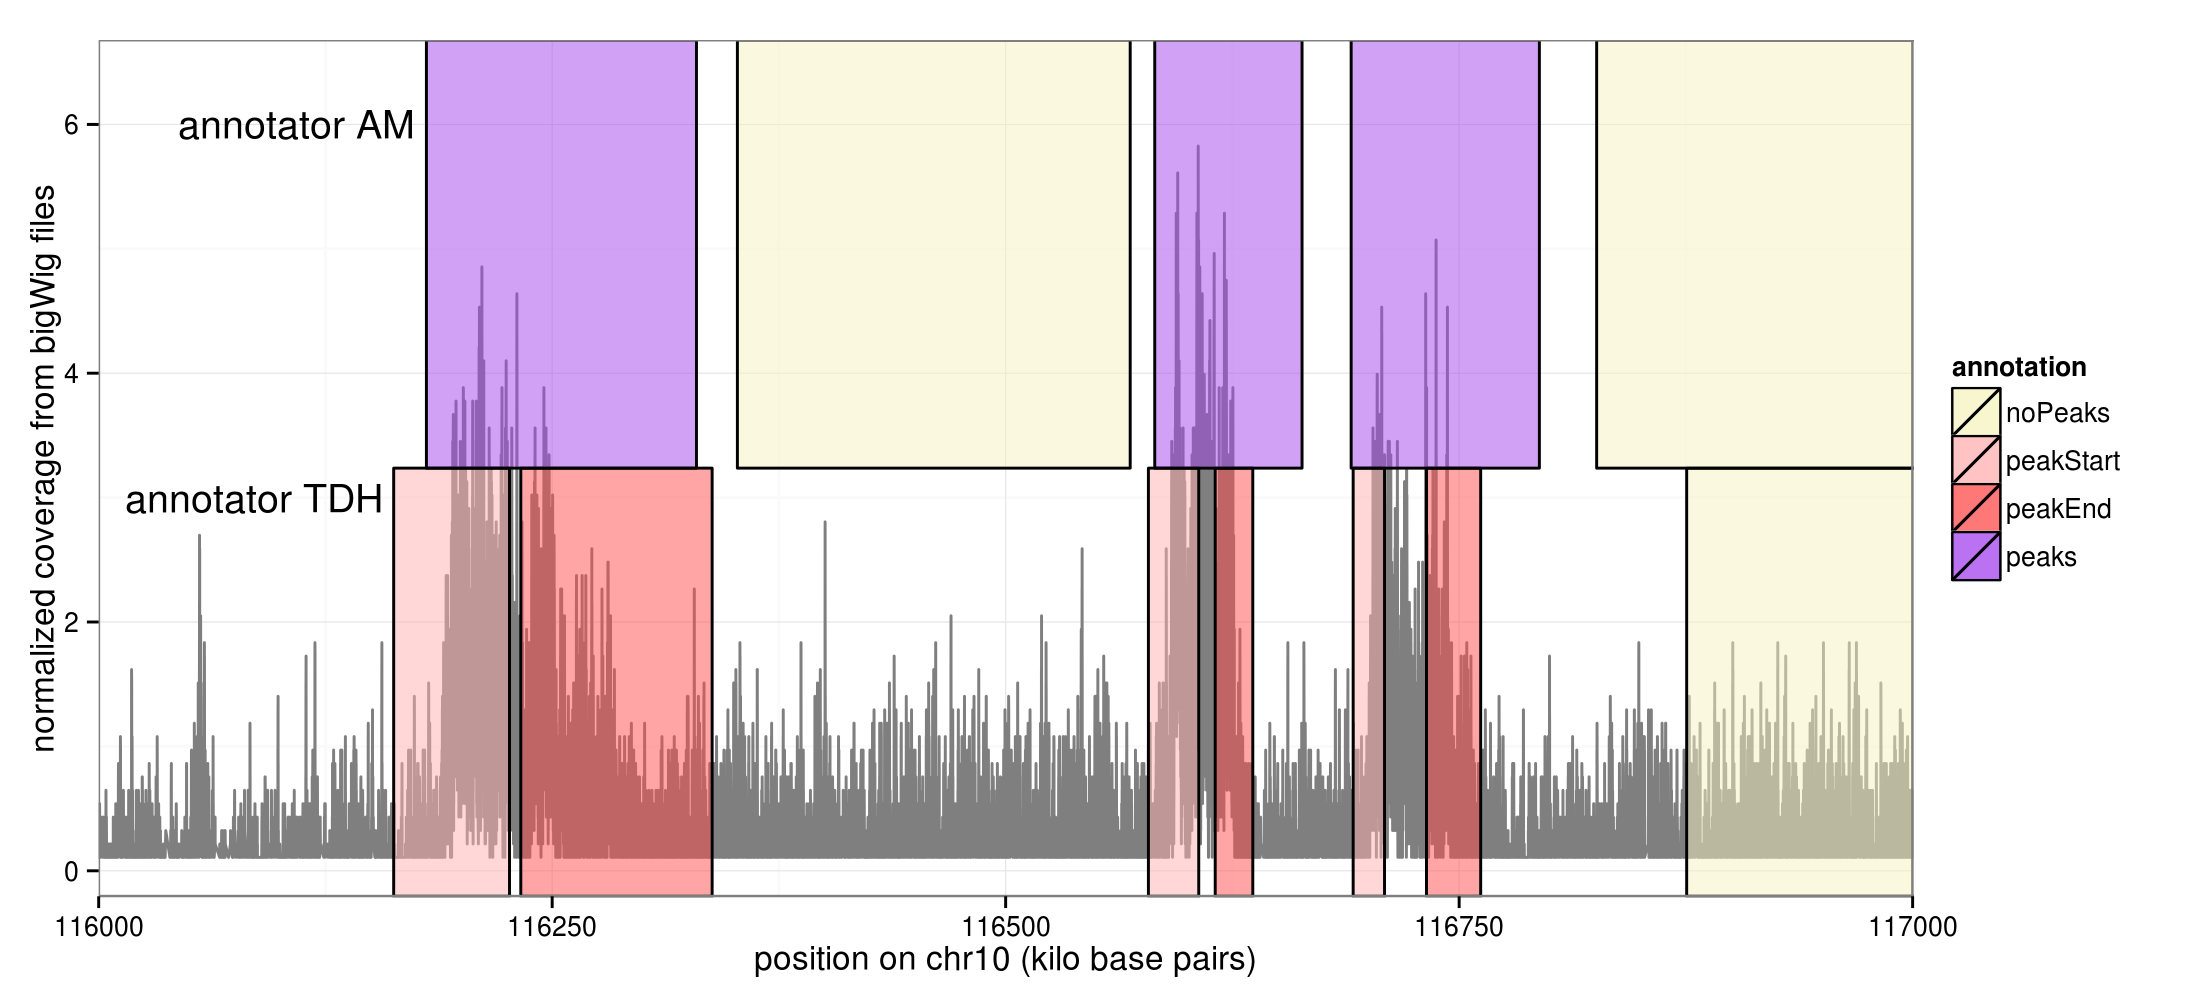
\includegraphics[width=1.1\textwidth]{screenshot-several-annotators}

  \begin{itemize}
  \item TDH peakStart/peakEnd more precise than AM peaks.
  \item AM noPeaks more precise than TDH no label.
  \end{itemize}
\end{frame}

\begin{frame}
  \frametitle{Models trained on labels from one person\\
predict accurately for another person\\
    (same histone mark and samples)}
  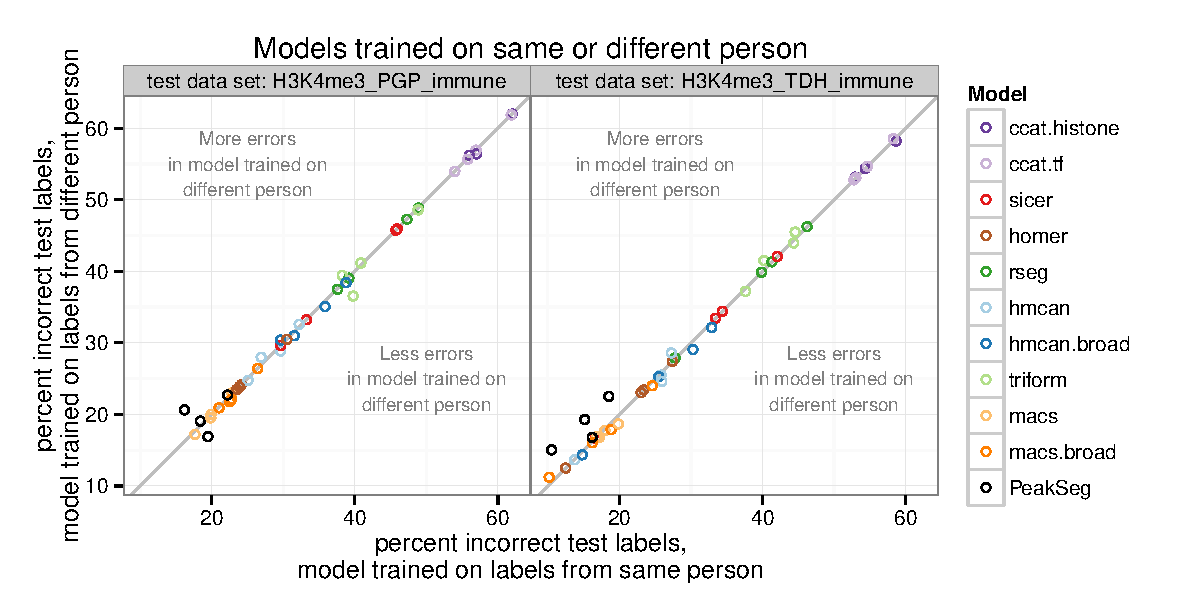
\includegraphics[width=1.1\textwidth]{figure-test-H3K4me3-annotators.pdf}

  Test error in four-fold cross-validation.
\end{frame}

\begin{frame}
  \frametitle{Only a few labels are required to train highly accurate models to recognize any peak pattern}
  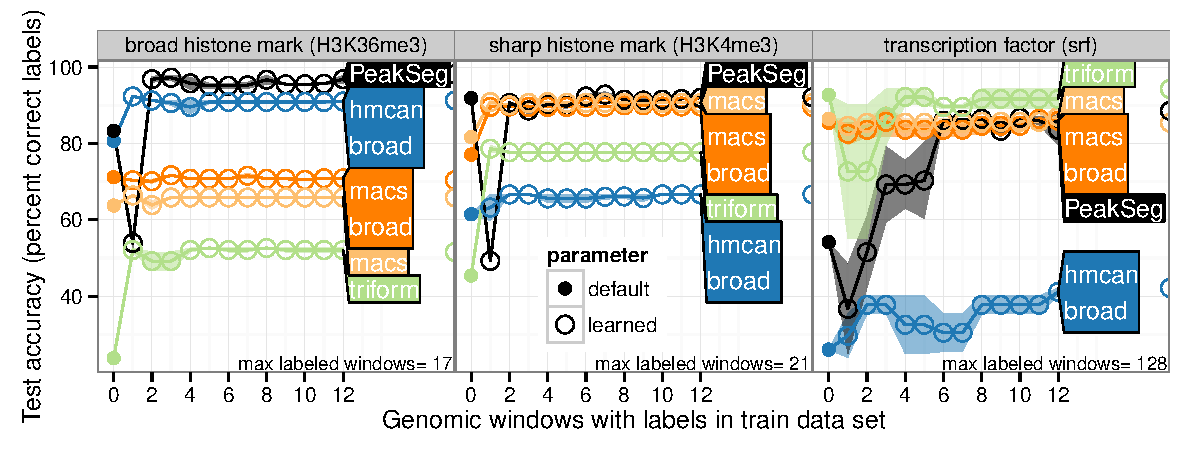
\includegraphics[width=1.1\textwidth]{figure-test-error-decreases-mean.pdf}
 
  \begin{itemize}
  \item Three different ChIP-seq experiments, each with a separate
    labeled pattern (broad/sharp/etc).
  \item Test accuracy quickly increases to max after 2--6
    genomic windows (containing several labeled regions and samples).
  \item PeakSeg highly accurate in all three patterns.
  \item Other models only accurate for only one or two patterns.
  \end{itemize}
\end{frame}

\begin{frame}
  \frametitle{Maximum likelihood changepoint detection with up-down constraints on adjacent segment means (PeakSeg)}
H {\it et al.}, {\it ICML} 2015. 
   
\only<1>{% Created by tikzDevice version 0.10.1 on 2017-11-02 21:08:21
% !TEX encoding = UTF-8 Unicode
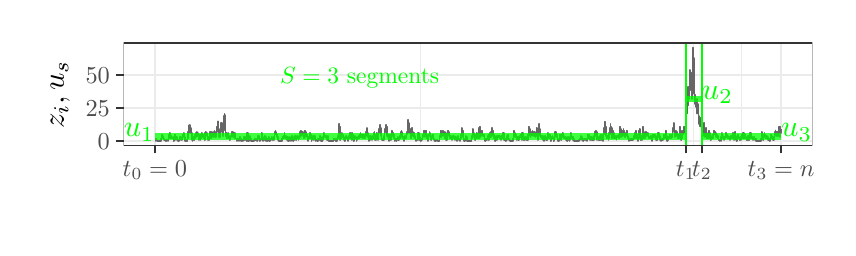
\begin{tikzpicture}[x=1pt,y=1pt]
\definecolor{fillColor}{RGB}{255,255,255}
\path[use as bounding box,fill=fillColor,fill opacity=0.00] (0,0) rectangle (289.08, 72.27);
\begin{scope}
\path[clip] (  0.00,  0.00) rectangle (289.08, 72.27);
\definecolor{drawColor}{RGB}{255,255,255}
\definecolor{fillColor}{RGB}{255,255,255}

\path[draw=drawColor,line width= 0.6pt,line join=round,line cap=round,fill=fillColor] (  0.00,  0.00) rectangle (289.08, 72.27);
\end{scope}
\begin{scope}
\path[clip] ( 34.65, 29.59) rectangle (283.58, 66.77);
\definecolor{fillColor}{RGB}{255,255,255}

\path[fill=fillColor] ( 34.65, 29.59) rectangle (283.58, 66.77);
\definecolor{drawColor}{gray}{0.92}

\path[draw=drawColor,line width= 0.3pt,line join=round] (141.89, 29.59) --
	(141.89, 66.77);

\path[draw=drawColor,line width= 0.3pt,line join=round] (240.71, 29.59) --
	(240.71, 66.77);

\path[draw=drawColor,line width= 0.3pt,line join=round] (257.94, 29.59) --
	(257.94, 66.77);

\path[draw=drawColor,line width= 0.6pt,line join=round] ( 34.65, 31.28) --
	(283.58, 31.28);

\path[draw=drawColor,line width= 0.6pt,line join=round] ( 34.65, 43.18) --
	(283.58, 43.18);

\path[draw=drawColor,line width= 0.6pt,line join=round] ( 34.65, 55.08) --
	(283.58, 55.08);

\path[draw=drawColor,line width= 0.6pt,line join=round] ( 45.97, 29.59) --
	( 45.97, 66.77);

\path[draw=drawColor,line width= 0.6pt,line join=round] (237.82, 29.59) --
	(237.82, 66.77);

\path[draw=drawColor,line width= 0.6pt,line join=round] (243.61, 29.59) --
	(243.61, 66.77);

\path[draw=drawColor,line width= 0.6pt,line join=round] (272.26, 29.59) --
	(272.26, 66.77);
\definecolor{drawColor}{gray}{0.40}

\path[draw=drawColor,line width= 0.6pt,line join=round] ( 45.97, 31.75) --
	( 46.15, 31.75) --
	( 46.15, 31.28) --
	( 46.17, 31.28) --
	( 46.17, 31.75) --
	( 46.18, 31.75) --
	( 46.18, 32.23) --
	( 46.60, 32.23) --
	( 46.60, 31.75) --
	( 46.63, 31.75) --
	( 46.63, 31.28) --
	( 48.22, 31.28) --
	( 48.22, 31.75) --
	( 48.26, 31.75) --
	( 48.26, 32.23) --
	( 48.49, 32.23) --
	( 48.49, 32.71) --
	( 48.56, 32.71) --
	( 48.56, 33.18) --
	( 48.63, 33.18) --
	( 48.63, 33.66) --
	( 48.67, 33.66) --
	( 48.67, 33.18) --
	( 48.71, 33.18) --
	( 48.71, 32.71) --
	( 48.83, 32.71) --
	( 48.83, 33.18) --
	( 48.94, 33.18) --
	( 48.94, 32.71) --
	( 49.00, 32.71) --
	( 49.00, 33.18) --
	( 49.01, 33.18) --
	( 49.01, 32.71) --
	( 49.08, 32.71) --
	( 49.08, 32.23) --
	( 49.29, 32.23) --
	( 49.29, 31.75) --
	( 49.31, 31.75) --
	( 49.31, 32.23) --
	( 49.45, 32.23) --
	( 49.45, 31.75) --
	( 49.76, 31.75) --
	( 49.76, 31.28) --
	( 50.20, 31.28) --
	( 50.20, 31.75) --
	( 50.65, 31.75) --
	( 50.65, 31.28) --
	( 50.68, 31.28) --
	( 50.68, 31.75) --
	( 50.86, 31.75) --
	( 50.86, 32.23) --
	( 50.96, 32.23) --
	( 50.96, 32.71) --
	( 51.04, 32.71) --
	( 51.04, 33.18) --
	( 51.06, 33.18) --
	( 51.06, 33.66) --
	( 51.14, 33.66) --
	( 51.14, 33.18) --
	( 51.20, 33.18) --
	( 51.20, 33.66) --
	( 51.30, 33.66) --
	( 51.30, 34.13) --
	( 51.31, 34.13) --
	( 51.31, 33.66) --
	( 51.32, 33.66) --
	( 51.32, 34.13) --
	( 51.41, 34.13) --
	( 51.41, 33.66) --
	( 51.47, 33.66) --
	( 51.47, 34.13) --
	( 51.50, 34.13) --
	( 51.50, 33.66) --
	( 51.51, 33.66) --
	( 51.51, 33.18) --
	( 51.53, 33.18) --
	( 51.53, 33.66) --
	( 51.65, 33.66) --
	( 51.65, 33.18) --
	( 51.75, 33.18) --
	( 51.75, 32.71) --
	( 51.77, 32.71) --
	( 51.77, 32.23) --
	( 51.80, 32.23) --
	( 51.80, 32.71) --
	( 51.82, 32.71) --
	( 51.82, 33.18) --
	( 51.93, 33.18) --
	( 51.93, 32.71) --
	( 51.97, 32.71) --
	( 51.97, 32.23) --
	( 52.26, 32.23) --
	( 52.26, 32.71) --
	( 52.27, 32.71) --
	( 52.27, 32.23) --
	( 52.70, 32.23) --
	( 52.70, 31.28) --
	( 52.81, 31.28) --
	( 52.81, 31.75) --
	( 52.83, 31.75) --
	( 52.83, 32.23) --
	( 52.88, 32.23) --
	( 52.88, 32.71) --
	( 53.02, 32.71) --
	( 53.02, 33.18) --
	( 53.10, 33.18) --
	( 53.10, 33.66) --
	( 53.26, 33.66) --
	( 53.26, 33.18) --
	( 53.29, 33.18) --
	( 53.29, 32.71) --
	( 53.34, 32.71) --
	( 53.34, 32.23) --
	( 53.34, 32.23) --
	( 53.34, 32.71) --
	( 53.47, 32.71) --
	( 53.47, 32.23) --
	( 53.55, 32.23) --
	( 53.55, 31.75) --
	( 53.60, 31.75) --
	( 53.60, 32.23) --
	( 53.69, 32.23) --
	( 53.69, 32.71) --
	( 53.79, 32.71) --
	( 53.79, 32.23) --
	( 53.98, 32.23) --
	( 53.98, 32.71) --
	( 54.05, 32.71) --
	( 54.05, 32.23) --
	( 54.14, 32.23) --
	( 54.14, 31.75) --
	( 54.43, 31.75) --
	( 54.43, 31.28) --
	( 54.79, 31.28) --
	( 54.79, 31.75) --
	( 55.03, 31.75) --
	( 55.03, 32.23) --
	( 55.09, 32.23) --
	( 55.09, 32.71) --
	( 55.25, 32.71) --
	( 55.25, 32.23) --
	( 55.35, 32.23) --
	( 55.35, 32.71) --
	( 55.48, 32.71) --
	( 55.48, 32.23) --
	( 55.54, 32.23) --
	( 55.54, 31.75) --
	( 55.78, 31.75) --
	( 55.78, 32.23) --
	( 55.80, 32.23) --
	( 55.80, 31.75) --
	( 55.81, 31.75) --
	( 55.81, 32.23) --
	( 55.98, 32.23) --
	( 55.98, 33.18) --
	( 56.17, 33.18) --
	( 56.17, 33.66) --
	( 56.23, 33.66) --
	( 56.23, 33.18) --
	( 56.27, 33.18) --
	( 56.27, 32.71) --
	( 56.41, 32.71) --
	( 56.41, 33.66) --
	( 56.43, 33.66) --
	( 56.43, 34.13) --
	( 56.44, 34.13) --
	( 56.44, 33.18) --
	( 56.62, 33.18) --
	( 56.62, 32.71) --
	( 56.87, 32.71) --
	( 56.87, 31.75) --
	( 56.87, 31.75) --
	( 56.87, 31.28) --
	( 57.13, 31.28) --
	( 57.13, 31.75) --
	( 57.59, 31.75) --
	( 57.59, 31.28) --
	( 57.72, 31.28) --
	( 57.72, 31.75) --
	( 57.77, 31.75) --
	( 57.77, 32.23) --
	( 57.82, 32.23) --
	( 57.82, 33.18) --
	( 57.91, 33.18) --
	( 57.91, 34.13) --
	( 58.05, 34.13) --
	( 58.05, 34.61) --
	( 58.10, 34.61) --
	( 58.10, 35.09) --
	( 58.17, 35.09) --
	( 58.17, 34.61) --
	( 58.20, 34.61) --
	( 58.20, 36.04) --
	( 58.22, 36.04) --
	( 58.22, 36.51) --
	( 58.22, 36.51) --
	( 58.22, 36.04) --
	( 58.27, 36.04) --
	( 58.27, 36.99) --
	( 58.27, 36.99) --
	( 58.27, 36.04) --
	( 58.34, 36.04) --
	( 58.34, 36.51) --
	( 58.37, 36.51) --
	( 58.37, 35.56) --
	( 58.43, 35.56) --
	( 58.43, 36.04) --
	( 58.51, 36.04) --
	( 58.51, 35.56) --
	( 58.56, 35.56) --
	( 58.56, 35.09) --
	( 58.59, 35.09) --
	( 58.59, 36.51) --
	( 58.64, 36.51) --
	( 58.64, 36.99) --
	( 58.65, 36.99) --
	( 58.65, 36.51) --
	( 58.65, 36.51) --
	( 58.65, 35.56) --
	( 58.67, 35.56) --
	( 58.67, 35.09) --
	( 58.73, 35.09) --
	( 58.73, 34.13) --
	( 58.81, 34.13) --
	( 58.81, 34.61) --
	( 58.84, 34.61) --
	( 58.84, 35.09) --
	( 58.84, 35.09) --
	( 58.84, 35.56) --
	( 58.89, 35.56) --
	( 58.89, 35.09) --
	( 58.99, 35.09) --
	( 58.99, 35.56) --
	( 59.02, 35.56) --
	( 59.02, 36.04) --
	( 59.04, 36.04) --
	( 59.04, 34.61) --
	( 59.05, 34.61) --
	( 59.05, 35.09) --
	( 59.09, 35.09) --
	( 59.09, 34.61) --
	( 59.25, 34.61) --
	( 59.25, 34.13) --
	( 59.27, 34.13) --
	( 59.27, 33.66) --
	( 59.29, 33.66) --
	( 59.29, 32.71) --
	( 59.45, 32.71) --
	( 59.45, 31.75) --
	( 59.51, 31.75) --
	( 59.51, 31.28) --
	( 59.56, 31.28) --
	( 59.56, 31.75) --
	( 59.65, 31.75) --
	( 59.65, 32.23) --
	( 59.87, 32.23) --
	( 59.87, 32.71) --
	( 60.00, 32.71) --
	( 60.00, 32.23) --
	( 60.10, 32.23) --
	( 60.10, 31.75) --
	( 60.22, 31.75) --
	( 60.22, 32.23) --
	( 60.32, 32.23) --
	( 60.32, 31.75) --
	( 60.33, 31.75) --
	( 60.33, 32.23) --
	( 60.37, 32.23) --
	( 60.37, 32.71) --
	( 60.39, 32.71) --
	( 60.39, 33.18) --
	( 60.56, 33.18) --
	( 60.56, 33.66) --
	( 60.67, 33.66) --
	( 60.67, 33.18) --
	( 60.69, 33.18) --
	( 60.69, 33.66) --
	( 60.78, 33.66) --
	( 60.78, 33.18) --
	( 60.82, 33.18) --
	( 60.82, 32.71) --
	( 60.83, 32.71) --
	( 60.83, 33.66) --
	( 60.85, 33.66) --
	( 60.85, 33.18) --
	( 60.92, 33.18) --
	( 60.92, 33.66) --
	( 60.94, 33.66) --
	( 60.94, 34.13) --
	( 61.09, 34.13) --
	( 61.09, 34.61) --
	( 61.14, 34.61) --
	( 61.14, 34.13) --
	( 61.23, 34.13) --
	( 61.23, 34.61) --
	( 61.28, 34.61) --
	( 61.28, 33.66) --
	( 61.37, 33.66) --
	( 61.37, 34.13) --
	( 61.38, 34.13) --
	( 61.38, 33.66) --
	( 61.39, 33.66) --
	( 61.39, 33.18) --
	( 61.42, 33.18) --
	( 61.42, 34.13) --
	( 61.46, 34.13) --
	( 61.46, 33.66) --
	( 61.54, 33.66) --
	( 61.54, 33.18) --
	( 61.68, 33.18) --
	( 61.68, 32.71) --
	( 61.79, 32.71) --
	( 61.79, 33.18) --
	( 61.82, 33.18) --
	( 61.82, 32.71) --
	( 61.88, 32.71) --
	( 61.88, 31.75) --
	( 61.89, 31.75) --
	( 61.89, 32.23) --
	( 61.91, 32.23) --
	( 61.91, 32.71) --
	( 61.96, 32.71) --
	( 61.96, 33.18) --
	( 62.22, 33.18) --
	( 62.22, 33.66) --
	( 62.23, 33.66) --
	( 62.23, 33.18) --
	( 62.34, 33.18) --
	( 62.34, 32.71) --
	( 62.36, 32.71) --
	( 62.36, 32.23) --
	( 62.42, 32.23) --
	( 62.42, 31.75) --
	( 62.50, 31.75) --
	( 62.50, 32.23) --
	( 62.61, 32.23) --
	( 62.61, 32.71) --
	( 62.63, 32.71) --
	( 62.63, 33.18) --
	( 62.64, 33.18) --
	( 62.64, 33.66) --
	( 62.66, 33.66) --
	( 62.66, 33.18) --
	( 62.68, 33.18) --
	( 62.68, 33.66) --
	( 62.75, 33.66) --
	( 62.75, 34.13) --
	( 62.95, 34.13) --
	( 62.95, 33.66) --
	( 63.03, 33.66) --
	( 63.03, 34.13) --
	( 63.09, 34.13) --
	( 63.09, 33.66) --
	( 63.09, 33.66) --
	( 63.09, 33.18) --
	( 63.10, 33.18) --
	( 63.10, 33.66) --
	( 63.14, 33.66) --
	( 63.14, 33.18) --
	( 63.20, 33.18) --
	( 63.20, 32.71) --
	( 63.42, 32.71) --
	( 63.42, 33.18) --
	( 63.45, 33.18) --
	( 63.45, 33.66) --
	( 63.48, 33.66) --
	( 63.48, 33.18) --
	( 63.51, 33.18) --
	( 63.51, 32.71) --
	( 63.55, 32.71) --
	( 63.55, 32.23) --
	( 63.86, 32.23) --
	( 63.86, 32.71) --
	( 63.87, 32.71) --
	( 63.87, 32.23) --
	( 63.91, 32.23) --
	( 63.91, 31.75) --
	( 63.96, 31.75) --
	( 63.96, 32.23) --
	( 63.97, 32.23) --
	( 63.97, 32.71) --
	( 64.06, 32.71) --
	( 64.06, 33.18) --
	( 64.14, 33.18) --
	( 64.14, 33.66) --
	( 64.17, 33.66) --
	( 64.17, 34.13) --
	( 64.25, 34.13) --
	( 64.25, 34.61) --
	( 64.31, 34.61) --
	( 64.31, 34.13) --
	( 64.39, 34.13) --
	( 64.39, 34.61) --
	( 64.41, 34.61) --
	( 64.41, 34.13) --
	( 64.42, 34.13) --
	( 64.42, 33.66) --
	( 64.48, 33.66) --
	( 64.48, 33.18) --
	( 64.52, 33.18) --
	( 64.52, 33.66) --
	( 64.58, 33.66) --
	( 64.58, 34.13) --
	( 64.59, 34.13) --
	( 64.59, 33.66) --
	( 64.60, 33.66) --
	( 64.60, 34.13) --
	( 64.62, 34.13) --
	( 64.62, 33.66) --
	( 64.65, 33.66) --
	( 64.65, 34.13) --
	( 64.71, 34.13) --
	( 64.71, 33.66) --
	( 64.76, 33.66) --
	( 64.76, 34.13) --
	( 64.85, 34.13) --
	( 64.85, 33.66) --
	( 64.97, 33.66) --
	( 64.97, 33.18) --
	( 65.04, 33.18) --
	( 65.04, 32.71) --
	( 65.05, 32.71) --
	( 65.05, 32.23) --
	( 65.10, 32.23) --
	( 65.10, 31.75) --
	( 65.13, 31.75) --
	( 65.13, 32.23) --
	( 65.15, 32.23) --
	( 65.15, 31.75) --
	( 65.28, 31.75) --
	( 65.28, 32.23) --
	( 65.53, 32.23) --
	( 65.53, 32.71) --
	( 65.58, 32.71) --
	( 65.58, 32.23) --
	( 65.73, 32.23) --
	( 65.73, 31.75) --
	( 65.76, 31.75) --
	( 65.76, 32.71) --
	( 65.78, 32.71) --
	( 65.78, 33.18) --
	( 65.80, 33.18) --
	( 65.80, 33.66) --
	( 65.82, 33.66) --
	( 65.82, 34.13) --
	( 65.86, 34.13) --
	( 65.86, 34.61) --
	( 65.98, 34.61) --
	( 65.98, 34.13) --
	( 66.05, 34.13) --
	( 66.05, 34.61) --
	( 66.21, 34.61) --
	( 66.21, 33.66) --
	( 66.24, 33.66) --
	( 66.24, 33.18) --
	( 66.24, 33.18) --
	( 66.24, 32.71) --
	( 66.31, 32.71) --
	( 66.31, 32.23) --
	( 66.39, 32.23) --
	( 66.39, 32.71) --
	( 66.41, 32.71) --
	( 66.41, 33.66) --
	( 66.53, 33.66) --
	( 66.53, 34.13) --
	( 66.58, 34.13) --
	( 66.58, 34.61) --
	( 66.72, 34.61) --
	( 66.72, 34.13) --
	( 66.84, 34.13) --
	( 66.84, 33.66) --
	( 66.86, 33.66) --
	( 66.86, 32.71) --
	( 66.89, 32.71) --
	( 66.89, 33.18) --
	( 66.96, 33.18) --
	( 66.96, 32.71) --
	( 66.98, 32.71) --
	( 66.98, 33.18) --
	( 66.99, 33.18) --
	( 66.99, 32.71) --
	( 67.02, 32.71) --
	( 67.02, 33.18) --
	( 67.03, 33.18) --
	( 67.03, 32.71) --
	( 67.09, 32.71) --
	( 67.09, 33.18) --
	( 67.16, 33.18) --
	( 67.16, 33.66) --
	( 67.19, 33.66) --
	( 67.19, 34.13) --
	( 67.27, 34.13) --
	( 67.27, 34.61) --
	( 67.34, 34.61) --
	( 67.34, 34.13) --
	( 67.34, 34.13) --
	( 67.34, 34.61) --
	( 67.43, 34.61) --
	( 67.43, 34.13) --
	( 67.46, 34.13) --
	( 67.46, 34.61) --
	( 67.47, 34.61) --
	( 67.47, 35.09) --
	( 67.48, 35.09) --
	( 67.48, 34.61) --
	( 67.54, 34.61) --
	( 67.54, 34.13) --
	( 67.62, 34.13) --
	( 67.62, 33.66) --
	( 67.64, 33.66) --
	( 67.64, 33.18) --
	( 67.72, 33.18) --
	( 67.72, 32.71) --
	( 67.73, 32.71) --
	( 67.73, 33.18) --
	( 67.76, 33.18) --
	( 67.76, 34.13) --
	( 67.80, 34.13) --
	( 67.80, 33.66) --
	( 67.91, 33.66) --
	( 67.91, 33.18) --
	( 67.92, 33.18) --
	( 67.92, 32.71) --
	( 67.94, 32.71) --
	( 67.94, 33.18) --
	( 67.99, 33.18) --
	( 67.99, 33.66) --
	( 68.06, 33.66) --
	( 68.06, 34.13) --
	( 68.16, 34.13) --
	( 68.16, 34.61) --
	( 68.18, 34.61) --
	( 68.18, 34.13) --
	( 68.20, 34.13) --
	( 68.20, 34.61) --
	( 68.20, 34.61) --
	( 68.20, 35.09) --
	( 68.21, 35.09) --
	( 68.21, 34.61) --
	( 68.21, 34.61) --
	( 68.21, 34.13) --
	( 68.24, 34.13) --
	( 68.24, 34.61) --
	( 68.39, 34.61) --
	( 68.39, 35.09) --
	( 68.39, 35.09) --
	( 68.39, 34.61) --
	( 68.44, 34.61) --
	( 68.44, 35.09) --
	( 68.44, 35.09) --
	( 68.44, 34.61) --
	( 68.46, 34.61) --
	( 68.46, 36.04) --
	( 68.47, 36.04) --
	( 68.47, 36.51) --
	( 68.49, 36.51) --
	( 68.49, 36.04) --
	( 68.51, 36.04) --
	( 68.51, 36.51) --
	( 68.56, 36.51) --
	( 68.56, 36.99) --
	( 68.60, 36.99) --
	( 68.60, 37.47) --
	( 68.61, 37.47) --
	( 68.61, 36.99) --
	( 68.65, 36.99) --
	( 68.65, 36.51) --
	( 68.66, 36.51) --
	( 68.66, 36.04) --
	( 68.66, 36.04) --
	( 68.66, 36.51) --
	( 68.69, 36.51) --
	( 68.69, 36.99) --
	( 68.69, 36.99) --
	( 68.69, 36.51) --
	( 68.70, 36.51) --
	( 68.70, 37.47) --
	( 68.77, 37.47) --
	( 68.77, 37.94) --
	( 68.83, 37.94) --
	( 68.83, 38.42) --
	( 68.83, 38.42) --
	( 68.83, 37.94) --
	( 68.89, 37.94) --
	( 68.89, 37.47) --
	( 68.92, 37.47) --
	( 68.92, 36.04) --
	( 68.92, 36.04) --
	( 68.92, 35.09) --
	( 68.93, 35.09) --
	( 68.93, 35.56) --
	( 68.99, 35.56) --
	( 68.99, 36.04) --
	( 69.01, 36.04) --
	( 69.01, 35.56) --
	( 69.05, 35.56) --
	( 69.05, 35.09) --
	( 69.06, 35.09) --
	( 69.06, 34.61) --
	( 69.14, 34.61) --
	( 69.14, 34.13) --
	( 69.16, 34.13) --
	( 69.16, 33.18) --
	( 69.20, 33.18) --
	( 69.20, 33.66) --
	( 69.21, 33.66) --
	( 69.21, 32.71) --
	( 69.30, 32.71) --
	( 69.30, 33.18) --
	( 69.38, 33.18) --
	( 69.38, 33.66) --
	( 69.39, 33.66) --
	( 69.39, 33.18) --
	( 69.44, 33.18) --
	( 69.44, 32.71) --
	( 69.51, 32.71) --
	( 69.51, 33.66) --
	( 69.55, 33.66) --
	( 69.55, 34.13) --
	( 69.59, 34.13) --
	( 69.59, 34.61) --
	( 69.59, 34.61) --
	( 69.59, 34.13) --
	( 69.66, 34.13) --
	( 69.66, 34.61) --
	( 69.68, 34.61) --
	( 69.68, 35.09) --
	( 69.75, 35.09) --
	( 69.75, 34.61) --
	( 69.78, 34.61) --
	( 69.78, 35.09) --
	( 69.79, 35.09) --
	( 69.79, 35.56) --
	( 69.82, 35.56) --
	( 69.82, 36.04) --
	( 69.85, 36.04) --
	( 69.85, 35.56) --
	( 69.87, 35.56) --
	( 69.87, 36.04) --
	( 69.90, 36.04) --
	( 69.90, 36.51) --
	( 69.92, 36.51) --
	( 69.92, 36.99) --
	( 69.92, 36.99) --
	( 69.92, 37.47) --
	( 69.97, 37.47) --
	( 69.97, 37.94) --
	( 70.00, 37.94) --
	( 70.00, 37.47) --
	( 70.02, 37.47) --
	( 70.02, 37.94) --
	( 70.04, 37.94) --
	( 70.04, 37.47) --
	( 70.05, 37.47) --
	( 70.05, 36.99) --
	( 70.08, 36.99) --
	( 70.08, 37.47) --
	( 70.09, 37.47) --
	( 70.09, 37.94) --
	( 70.11, 37.94) --
	( 70.11, 37.47) --
	( 70.19, 37.47) --
	( 70.19, 37.94) --
	( 70.24, 37.94) --
	( 70.24, 37.47) --
	( 70.27, 37.47) --
	( 70.27, 36.99) --
	( 70.28, 36.99) --
	( 70.28, 37.47) --
	( 70.29, 37.47) --
	( 70.29, 36.99) --
	( 70.32, 36.99) --
	( 70.32, 37.47) --
	( 70.35, 37.47) --
	( 70.35, 36.99) --
	( 70.37, 36.99) --
	( 70.37, 36.51) --
	( 70.38, 36.51) --
	( 70.38, 36.04) --
	( 70.41, 36.04) --
	( 70.41, 35.56) --
	( 70.43, 35.56) --
	( 70.43, 35.09) --
	( 70.47, 35.09) --
	( 70.47, 34.61) --
	( 70.52, 34.61) --
	( 70.52, 34.13) --
	( 70.53, 34.13) --
	( 70.53, 34.61) --
	( 70.54, 34.61) --
	( 70.54, 34.13) --
	( 70.54, 34.13) --
	( 70.54, 33.66) --
	( 70.59, 33.66) --
	( 70.59, 33.18) --
	( 70.60, 33.18) --
	( 70.60, 33.66) --
	( 70.63, 33.66) --
	( 70.63, 34.13) --
	( 70.64, 34.13) --
	( 70.64, 33.66) --
	( 70.72, 33.66) --
	( 70.72, 34.13) --
	( 70.73, 34.13) --
	( 70.73, 33.66) --
	( 70.77, 33.66) --
	( 70.77, 33.18) --
	( 70.79, 33.18) --
	( 70.79, 33.66) --
	( 70.79, 33.66) --
	( 70.79, 34.61) --
	( 70.80, 34.61) --
	( 70.80, 35.09) --
	( 70.86, 35.09) --
	( 70.86, 35.56) --
	( 70.89, 35.56) --
	( 70.89, 36.04) --
	( 70.91, 36.04) --
	( 70.91, 36.51) --
	( 70.91, 36.51) --
	( 70.91, 36.99) --
	( 70.95, 36.99) --
	( 70.95, 37.47) --
	( 70.97, 37.47) --
	( 70.97, 37.94) --
	( 70.98, 37.94) --
	( 70.98, 37.47) --
	( 70.98, 37.47) --
	( 70.98, 37.94) --
	( 71.00, 37.94) --
	( 71.00, 39.37) --
	( 71.02, 39.37) --
	( 71.02, 39.85) --
	( 71.04, 39.85) --
	( 71.04, 39.37) --
	( 71.05, 39.37) --
	( 71.05, 39.85) --
	( 71.06, 39.85) --
	( 71.06, 40.32) --
	( 71.07, 40.32) --
	( 71.07, 40.80) --
	( 71.08, 40.80) --
	( 71.08, 41.27) --
	( 71.09, 41.27) --
	( 71.09, 40.80) --
	( 71.14, 40.80) --
	( 71.14, 41.27) --
	( 71.17, 41.27) --
	( 71.17, 40.80) --
	( 71.24, 40.80) --
	( 71.24, 40.32) --
	( 71.25, 40.32) --
	( 71.25, 39.85) --
	( 71.26, 39.85) --
	( 71.26, 39.37) --
	( 71.31, 39.37) --
	( 71.31, 38.89) --
	( 71.35, 38.89) --
	( 71.35, 38.42) --
	( 71.36, 38.42) --
	( 71.36, 37.94) --
	( 71.36, 37.94) --
	( 71.36, 37.47) --
	( 71.40, 37.47) --
	( 71.40, 36.99) --
	( 71.42, 36.99) --
	( 71.42, 36.51) --
	( 71.44, 36.51) --
	( 71.44, 36.04) --
	( 71.45, 36.04) --
	( 71.45, 34.61) --
	( 71.46, 34.61) --
	( 71.46, 35.09) --
	( 71.47, 35.09) --
	( 71.47, 34.13) --
	( 71.50, 34.13) --
	( 71.50, 33.66) --
	( 71.51, 33.66) --
	( 71.51, 33.18) --
	( 71.52, 33.18) --
	( 71.52, 33.66) --
	( 71.53, 33.66) --
	( 71.53, 34.13) --
	( 71.54, 34.13) --
	( 71.54, 33.66) --
	( 71.59, 33.66) --
	( 71.59, 33.18) --
	( 71.71, 33.18) --
	( 71.71, 34.13) --
	( 71.91, 34.13) --
	( 71.91, 33.66) --
	( 71.97, 33.66) --
	( 71.97, 32.23) --
	( 72.14, 32.23) --
	( 72.14, 33.18) --
	( 72.16, 33.18) --
	( 72.16, 32.23) --
	( 72.25, 32.23) --
	( 72.25, 32.71) --
	( 72.38, 32.71) --
	( 72.38, 33.18) --
	( 72.52, 33.18) --
	( 72.52, 33.66) --
	( 72.53, 33.66) --
	( 72.53, 34.13) --
	( 72.59, 34.13) --
	( 72.59, 33.18) --
	( 72.69, 33.18) --
	( 72.69, 32.71) --
	( 72.83, 32.71) --
	( 72.83, 32.23) --
	( 72.84, 32.23) --
	( 72.84, 32.71) --
	( 72.97, 32.71) --
	( 72.97, 32.23) --
	( 72.98, 32.23) --
	( 72.98, 31.75) --
	( 73.00, 31.75) --
	( 73.00, 32.23) --
	( 73.01, 32.23) --
	( 73.01, 32.71) --
	( 73.28, 32.71) --
	( 73.28, 33.18) --
	( 73.29, 33.18) --
	( 73.29, 32.71) --
	( 73.43, 32.71) --
	( 73.43, 33.18) --
	( 73.46, 33.18) --
	( 73.46, 32.71) --
	( 73.53, 32.71) --
	( 73.53, 33.18) --
	( 73.66, 33.18) --
	( 73.66, 33.66) --
	( 73.73, 33.66) --
	( 73.73, 33.18) --
	( 73.77, 33.18) --
	( 73.77, 33.66) --
	( 73.83, 33.66) --
	( 73.83, 34.61) --
	( 73.88, 34.61) --
	( 73.88, 34.13) --
	( 73.91, 34.13) --
	( 73.91, 33.66) --
	( 73.98, 33.66) --
	( 73.98, 33.18) --
	( 74.03, 33.18) --
	( 74.03, 33.66) --
	( 74.05, 33.66) --
	( 74.05, 34.13) --
	( 74.11, 34.13) --
	( 74.11, 33.66) --
	( 74.16, 33.66) --
	( 74.16, 34.13) --
	( 74.20, 34.13) --
	( 74.20, 34.61) --
	( 74.21, 34.61) --
	( 74.21, 34.13) --
	( 74.21, 34.13) --
	( 74.21, 33.66) --
	( 74.24, 33.66) --
	( 74.24, 33.18) --
	( 74.28, 33.18) --
	( 74.28, 32.71) --
	( 74.36, 32.71) --
	( 74.36, 33.18) --
	( 74.38, 33.18) --
	( 74.38, 33.66) --
	( 74.41, 33.66) --
	( 74.41, 33.18) --
	( 74.50, 33.18) --
	( 74.50, 32.71) --
	( 74.52, 32.71) --
	( 74.52, 33.18) --
	( 74.52, 33.18) --
	( 74.52, 33.66) --
	( 74.62, 33.66) --
	( 74.62, 34.13) --
	( 74.65, 34.13) --
	( 74.65, 33.66) --
	( 74.65, 33.66) --
	( 74.65, 34.13) --
	( 74.81, 34.13) --
	( 74.81, 33.66) --
	( 74.83, 33.66) --
	( 74.83, 33.18) --
	( 74.97, 33.18) --
	( 74.97, 32.23) --
	( 75.05, 32.23) --
	( 75.05, 32.71) --
	( 75.07, 32.71) --
	( 75.07, 32.23) --
	( 75.08, 32.23) --
	( 75.08, 32.71) --
	( 75.10, 32.71) --
	( 75.10, 32.23) --
	( 75.50, 32.23) --
	( 75.50, 31.75) --
	( 75.53, 31.75) --
	( 75.53, 31.28) --
	( 75.72, 31.28) --
	( 75.72, 31.75) --
	( 75.83, 31.75) --
	( 75.83, 32.23) --
	( 76.12, 32.23) --
	( 76.12, 31.75) --
	( 76.28, 31.75) --
	( 76.28, 31.28) --
	( 76.47, 31.28) --
	( 76.47, 31.75) --
	( 76.53, 31.75) --
	( 76.53, 32.23) --
	( 76.54, 32.23) --
	( 76.54, 32.71) --
	( 76.92, 32.71) --
	( 76.92, 32.23) --
	( 76.98, 32.23) --
	( 76.98, 31.75) --
	( 76.99, 31.75) --
	( 76.99, 31.28) --
	( 77.22, 31.28) --
	( 77.22, 31.75) --
	( 77.68, 31.75) --
	( 77.68, 31.28) --
	( 77.89, 31.28) --
	( 77.89, 31.75) --
	( 78.03, 31.75) --
	( 78.03, 32.23) --
	( 78.20, 32.23) --
	( 78.20, 32.71) --
	( 78.24, 32.71) --
	( 78.24, 32.23) --
	( 78.35, 32.23) --
	( 78.35, 31.75) --
	( 78.51, 31.75) --
	( 78.51, 32.23) --
	( 78.57, 32.23) --
	( 78.57, 32.71) --
	( 78.65, 32.71) --
	( 78.65, 32.23) --
	( 78.96, 32.23) --
	( 78.96, 31.75) --
	( 79.02, 31.75) --
	( 79.02, 31.28) --
	( 79.20, 31.28) --
	( 79.20, 32.71) --
	( 79.23, 32.71) --
	( 79.23, 34.13) --
	( 79.65, 34.13) --
	( 79.65, 32.71) --
	( 79.68, 32.71) --
	( 79.68, 32.23) --
	( 79.68, 32.23) --
	( 79.68, 31.28) --
	( 79.93, 31.28) --
	( 79.93, 31.75) --
	( 79.96, 31.75) --
	( 79.96, 32.23) --
	( 80.14, 32.23) --
	( 80.14, 32.71) --
	( 80.29, 32.71) --
	( 80.29, 33.18) --
	( 80.35, 33.18) --
	( 80.35, 32.71) --
	( 80.41, 32.71) --
	( 80.41, 32.23) --
	( 80.59, 32.23) --
	( 80.59, 31.75) --
	( 80.74, 31.75) --
	( 80.74, 31.28) --
	( 81.79, 31.28) --
	( 81.79, 31.75) --
	( 82.03, 31.75) --
	( 82.03, 32.23) --
	( 82.24, 32.23) --
	( 82.24, 31.75) --
	( 82.27, 31.75) --
	( 82.27, 32.23) --
	( 82.48, 32.23) --
	( 82.48, 31.75) --
	( 82.53, 31.75) --
	( 82.53, 32.23) --
	( 82.72, 32.23) --
	( 82.72, 31.75) --
	( 82.98, 31.75) --
	( 82.98, 31.28) --
	( 83.02, 31.28) --
	( 83.02, 31.75) --
	( 83.25, 31.75) --
	( 83.25, 32.23) --
	( 83.28, 32.23) --
	( 83.28, 32.71) --
	( 83.29, 32.71) --
	( 83.29, 33.18) --
	( 83.47, 33.18) --
	( 83.47, 32.71) --
	( 83.71, 32.71) --
	( 83.71, 32.23) --
	( 83.73, 32.23) --
	( 83.73, 31.75) --
	( 83.74, 31.75) --
	( 83.74, 31.28) --
	( 83.85, 31.28) --
	( 83.85, 31.75) --
	( 84.23, 31.75) --
	( 84.23, 32.23) --
	( 84.30, 32.23) --
	( 84.30, 31.75) --
	( 84.38, 31.75) --
	( 84.38, 32.23) --
	( 84.46, 32.23) --
	( 84.46, 32.71) --
	( 84.49, 32.71) --
	( 84.49, 33.66) --
	( 84.51, 33.66) --
	( 84.51, 34.13) --
	( 84.68, 34.13) --
	( 84.68, 33.66) --
	( 84.83, 33.66) --
	( 84.83, 33.18) --
	( 84.91, 33.18) --
	( 84.91, 32.71) --
	( 84.95, 32.71) --
	( 84.95, 31.75) --
	( 84.96, 31.75) --
	( 84.96, 31.28) --
	( 84.99, 31.28) --
	( 84.99, 31.75) --
	( 85.22, 31.75) --
	( 85.22, 32.23) --
	( 85.44, 32.23) --
	( 85.44, 31.75) --
	( 85.57, 31.75) --
	( 85.57, 32.23) --
	( 85.63, 32.23) --
	( 85.63, 33.18) --
	( 85.67, 33.18) --
	( 85.67, 32.71) --
	( 86.02, 32.71) --
	( 86.02, 32.23) --
	( 86.08, 32.23) --
	( 86.08, 31.28) --
	( 86.14, 31.28) --
	( 86.14, 31.75) --
	( 86.38, 31.75) --
	( 86.38, 32.23) --
	( 86.59, 32.23) --
	( 86.59, 31.28) --
	( 86.66, 31.28) --
	( 86.66, 31.75) --
	( 86.80, 31.75) --
	( 86.80, 32.23) --
	( 87.05, 32.23) --
	( 87.05, 32.71) --
	( 87.09, 32.71) --
	( 87.09, 32.23) --
	( 87.24, 32.23) --
	( 87.24, 31.28) --
	( 87.50, 31.28) --
	( 87.50, 31.75) --
	( 87.93, 31.75) --
	( 87.93, 32.23) --
	( 87.95, 32.23) --
	( 87.95, 31.75) --
	( 88.03, 31.75) --
	( 88.03, 32.23) --
	( 88.20, 32.23) --
	( 88.20, 32.71) --
	( 88.38, 32.71) --
	( 88.38, 32.23) --
	( 88.49, 32.23) --
	( 88.49, 31.75) --
	( 88.50, 31.75) --
	( 88.50, 32.23) --
	( 88.63, 32.23) --
	( 88.63, 31.75) --
	( 88.76, 31.75) --
	( 88.76, 32.23) --
	( 88.95, 32.23) --
	( 88.95, 31.75) --
	( 89.11, 31.75) --
	( 89.11, 32.23) --
	( 89.12, 32.23) --
	( 89.12, 32.71) --
	( 89.17, 32.71) --
	( 89.17, 33.66) --
	( 89.21, 33.66) --
	( 89.21, 33.18) --
	( 89.25, 33.18) --
	( 89.25, 33.66) --
	( 89.28, 33.66) --
	( 89.28, 34.13) --
	( 89.39, 34.13) --
	( 89.39, 34.61) --
	( 89.50, 34.61) --
	( 89.50, 35.09) --
	( 89.56, 35.09) --
	( 89.56, 34.61) --
	( 89.57, 34.61) --
	( 89.57, 35.09) --
	( 89.58, 35.09) --
	( 89.58, 34.61) --
	( 89.63, 34.61) --
	( 89.63, 33.66) --
	( 89.69, 33.66) --
	( 89.69, 34.13) --
	( 89.70, 34.13) --
	( 89.70, 33.66) --
	( 89.71, 33.66) --
	( 89.71, 34.13) --
	( 89.73, 34.13) --
	( 89.73, 33.66) --
	( 89.81, 33.66) --
	( 89.81, 34.13) --
	( 89.84, 34.13) --
	( 89.84, 33.66) --
	( 89.95, 33.66) --
	( 89.95, 33.18) --
	( 89.99, 33.18) --
	( 89.99, 33.66) --
	( 90.02, 33.66) --
	( 90.02, 33.18) --
	( 90.08, 33.18) --
	( 90.08, 33.66) --
	( 90.15, 33.66) --
	( 90.15, 33.18) --
	( 90.15, 33.18) --
	( 90.15, 32.71) --
	( 90.22, 32.71) --
	( 90.22, 33.18) --
	( 90.26, 33.18) --
	( 90.26, 32.71) --
	( 90.44, 32.71) --
	( 90.44, 32.23) --
	( 90.54, 32.23) --
	( 90.54, 31.75) --
	( 90.68, 31.75) --
	( 90.68, 31.28) --
	( 91.91, 31.28) --
	( 91.91, 31.75) --
	( 91.93, 31.75) --
	( 91.93, 32.23) --
	( 92.07, 32.23) --
	( 92.07, 32.71) --
	( 92.35, 32.71) --
	( 92.35, 32.23) --
	( 92.36, 32.23) --
	( 92.36, 32.71) --
	( 92.38, 32.71) --
	( 92.38, 33.18) --
	( 92.39, 33.18) --
	( 92.39, 32.71) --
	( 92.53, 32.71) --
	( 92.53, 32.23) --
	( 92.61, 32.23) --
	( 92.61, 32.71) --
	( 92.69, 32.71) --
	( 92.69, 33.18) --
	( 92.79, 33.18) --
	( 92.79, 34.13) --
	( 92.81, 34.13) --
	( 92.81, 33.66) --
	( 92.83, 33.66) --
	( 92.83, 33.18) --
	( 93.07, 33.18) --
	( 93.07, 32.71) --
	( 93.11, 32.71) --
	( 93.11, 33.18) --
	( 93.14, 33.18) --
	( 93.14, 32.71) --
	( 93.16, 32.71) --
	( 93.16, 33.18) --
	( 93.24, 33.18) --
	( 93.24, 32.23) --
	( 93.52, 32.23) --
	( 93.52, 32.71) --
	( 93.56, 32.71) --
	( 93.56, 32.23) --
	( 93.61, 32.23) --
	( 93.61, 31.75) --
	( 93.64, 31.75) --
	( 93.64, 32.23) --
	( 93.72, 32.23) --
	( 93.72, 32.71) --
	( 93.97, 32.71) --
	( 93.97, 32.23) --
	( 94.09, 32.23) --
	( 94.09, 31.75) --
	( 94.17, 31.75) --
	( 94.17, 31.28) --
	( 94.42, 31.28) --
	( 94.42, 31.75) --
	( 94.42, 31.75) --
	( 94.42, 32.23) --
	( 94.75, 32.23) --
	( 94.75, 32.71) --
	( 94.87, 32.71) --
	( 94.87, 31.75) --
	( 95.20, 31.75) --
	( 95.20, 31.28) --
	( 95.22, 31.28) --
	( 95.22, 31.75) --
	( 95.39, 31.75) --
	( 95.39, 32.23) --
	( 95.47, 32.23) --
	( 95.47, 32.71) --
	( 95.50, 32.71) --
	( 95.50, 33.18) --
	( 95.67, 33.18) --
	( 95.67, 32.71) --
	( 95.84, 32.71) --
	( 95.84, 32.23) --
	( 95.92, 32.23) --
	( 95.92, 31.75) --
	( 95.95, 31.75) --
	( 95.95, 31.28) --
	( 96.00, 31.28) --
	( 96.00, 31.75) --
	( 96.37, 31.75) --
	( 96.37, 32.23) --
	( 96.44, 32.23) --
	( 96.44, 32.71) --
	( 96.45, 32.71) --
	( 96.45, 32.23) --
	( 96.46, 32.23) --
	( 96.46, 32.71) --
	( 96.56, 32.71) --
	( 96.56, 33.18) --
	( 96.82, 33.18) --
	( 96.82, 32.71) --
	( 96.84, 32.71) --
	( 96.84, 33.18) --
	( 96.89, 33.18) --
	( 96.89, 32.71) --
	( 96.90, 32.71) --
	( 96.90, 32.23) --
	( 97.01, 32.23) --
	( 97.01, 31.75) --
	( 97.14, 31.75) --
	( 97.14, 32.23) --
	( 97.22, 32.23) --
	( 97.22, 32.71) --
	( 97.30, 32.71) --
	( 97.30, 32.23) --
	( 97.36, 32.23) --
	( 97.36, 32.71) --
	( 97.44, 32.71) --
	( 97.44, 33.18) --
	( 97.58, 33.18) --
	( 97.58, 32.71) --
	( 97.60, 32.71) --
	( 97.60, 33.18) --
	( 97.67, 33.18) --
	( 97.67, 32.71) --
	( 97.81, 32.71) --
	( 97.81, 32.23) --
	( 97.89, 32.23) --
	( 97.89, 31.75) --
	( 97.92, 31.75) --
	( 97.92, 32.23) --
	( 97.95, 32.23) --
	( 97.95, 32.71) --
	( 98.06, 32.71) --
	( 98.06, 32.23) --
	( 98.11, 32.23) --
	( 98.11, 32.71) --
	( 98.19, 32.71) --
	( 98.19, 32.23) --
	( 98.21, 32.23) --
	( 98.21, 32.71) --
	( 98.32, 32.71) --
	( 98.32, 33.18) --
	( 98.36, 33.18) --
	( 98.36, 33.66) --
	( 98.42, 33.66) --
	( 98.42, 34.13) --
	( 98.51, 34.13) --
	( 98.51, 34.61) --
	( 98.56, 34.61) --
	( 98.56, 34.13) --
	( 98.65, 34.13) --
	( 98.65, 33.66) --
	( 98.70, 33.66) --
	( 98.70, 34.13) --
	( 98.70, 34.13) --
	( 98.70, 34.61) --
	( 98.76, 34.61) --
	( 98.76, 35.09) --
	( 98.77, 35.09) --
	( 98.77, 34.61) --
	( 98.81, 34.61) --
	( 98.81, 34.13) --
	( 98.84, 34.13) --
	( 98.84, 34.61) --
	( 98.85, 34.61) --
	( 98.85, 33.66) --
	( 98.96, 33.66) --
	( 98.96, 33.18) --
	( 98.96, 33.18) --
	( 98.96, 33.66) --
	( 99.12, 33.66) --
	( 99.12, 34.13) --
	( 99.15, 34.13) --
	( 99.15, 33.66) --
	( 99.16, 33.66) --
	( 99.16, 33.18) --
	( 99.16, 33.18) --
	( 99.16, 33.66) --
	( 99.19, 33.66) --
	( 99.19, 34.13) --
	( 99.21, 34.13) --
	( 99.21, 34.61) --
	( 99.22, 34.61) --
	( 99.22, 34.13) --
	( 99.25, 34.13) --
	( 99.25, 34.61) --
	( 99.29, 34.61) --
	( 99.29, 34.13) --
	( 99.39, 34.13) --
	( 99.39, 34.61) --
	( 99.41, 34.61) --
	( 99.41, 34.13) --
	( 99.50, 34.13) --
	( 99.50, 34.61) --
	( 99.57, 34.61) --
	( 99.57, 34.13) --
	( 99.61, 34.13) --
	( 99.61, 33.66) --
	( 99.64, 33.66) --
	( 99.64, 33.18) --
	( 99.65, 33.18) --
	( 99.65, 33.66) --
	( 99.70, 33.66) --
	( 99.70, 33.18) --
	( 99.84, 33.18) --
	( 99.84, 32.71) --
	( 99.86, 32.71) --
	( 99.86, 32.23) --
	( 99.89, 32.23) --
	( 99.89, 32.71) --
	( 99.89, 32.71) --
	( 99.89, 33.18) --
	(100.10, 33.18) --
	(100.10, 32.71) --
	(100.18, 32.71) --
	(100.18, 33.18) --
	(100.24, 33.18) --
	(100.24, 33.66) --
	(100.26, 33.66) --
	(100.26, 34.13) --
	(100.32, 34.13) --
	(100.32, 35.09) --
	(100.34, 35.09) --
	(100.34, 34.61) --
	(100.34, 34.61) --
	(100.34, 34.13) --
	(100.38, 34.13) --
	(100.38, 34.61) --
	(100.40, 34.61) --
	(100.40, 34.13) --
	(100.49, 34.13) --
	(100.49, 34.61) --
	(100.63, 34.61) --
	(100.63, 34.13) --
	(100.68, 34.13) --
	(100.68, 33.66) --
	(100.71, 33.66) --
	(100.71, 33.18) --
	(100.74, 33.18) --
	(100.74, 34.13) --
	(100.77, 34.13) --
	(100.77, 33.66) --
	(100.77, 33.66) --
	(100.77, 33.18) --
	(100.78, 33.18) --
	(100.78, 33.66) --
	(100.83, 33.66) --
	(100.83, 33.18) --
	(100.94, 33.18) --
	(100.94, 32.71) --
	(101.19, 32.71) --
	(101.19, 31.75) --
	(101.23, 31.75) --
	(101.23, 31.28) --
	(101.29, 31.28) --
	(101.29, 31.75) --
	(101.52, 31.75) --
	(101.52, 32.23) --
	(101.68, 32.23) --
	(101.68, 32.71) --
	(101.75, 32.71) --
	(101.75, 32.23) --
	(101.93, 32.23) --
	(101.93, 33.18) --
	(101.97, 33.18) --
	(101.97, 32.71) --
	(101.98, 32.71) --
	(101.98, 33.66) --
	(102.05, 33.66) --
	(102.05, 34.13) --
	(102.14, 34.13) --
	(102.14, 33.66) --
	(102.16, 33.66) --
	(102.16, 33.18) --
	(102.19, 33.18) --
	(102.19, 33.66) --
	(102.38, 33.66) --
	(102.38, 33.18) --
	(102.43, 33.18) --
	(102.43, 32.71) --
	(102.43, 32.71) --
	(102.43, 32.23) --
	(102.51, 32.23) --
	(102.51, 31.28) --
	(102.51, 31.28) --
	(102.51, 31.75) --
	(102.68, 31.75) --
	(102.68, 32.23) --
	(102.81, 32.23) --
	(102.81, 32.71) --
	(102.85, 32.71) --
	(102.85, 33.18) --
	(102.96, 33.18) --
	(102.96, 32.71) --
	(103.14, 32.71) --
	(103.14, 32.23) --
	(103.26, 32.23) --
	(103.26, 31.75) --
	(103.29, 31.75) --
	(103.29, 32.23) --
	(103.33, 32.23) --
	(103.33, 32.71) --
	(103.55, 32.71) --
	(103.55, 33.18) --
	(103.75, 33.18) --
	(103.75, 32.71) --
	(103.76, 32.71) --
	(103.76, 32.23) --
	(103.78, 32.23) --
	(103.78, 31.75) --
	(104.00, 31.75) --
	(104.00, 31.28) --
	(104.01, 31.28) --
	(104.01, 31.75) --
	(104.47, 31.75) --
	(104.47, 31.28) --
	(104.81, 31.28) --
	(104.81, 31.75) --
	(105.00, 31.75) --
	(105.00, 32.23) --
	(105.13, 32.23) --
	(105.13, 31.75) --
	(105.41, 31.75) --
	(105.41, 32.23) --
	(105.45, 32.23) --
	(105.45, 31.75) --
	(105.46, 31.75) --
	(105.46, 32.23) --
	(105.49, 32.23) --
	(105.49, 32.71) --
	(105.63, 32.71) --
	(105.63, 33.18) --
	(105.86, 33.18) --
	(105.86, 32.71) --
	(105.91, 32.71) --
	(105.91, 32.23) --
	(105.95, 32.23) --
	(105.95, 31.75) --
	(106.08, 31.75) --
	(106.08, 31.28) --
	(106.54, 31.28) --
	(106.54, 31.75) --
	(106.70, 31.75) --
	(106.70, 32.23) --
	(106.79, 32.23) --
	(106.79, 32.71) --
	(106.85, 32.71) --
	(106.85, 33.18) --
	(106.91, 33.18) --
	(106.91, 33.66) --
	(106.99, 33.66) --
	(106.99, 33.18) --
	(107.11, 33.18) --
	(107.11, 33.66) --
	(107.14, 33.66) --
	(107.14, 34.13) --
	(107.15, 34.13) --
	(107.15, 33.66) --
	(107.24, 33.66) --
	(107.24, 33.18) --
	(107.30, 33.18) --
	(107.30, 32.71) --
	(107.35, 32.71) --
	(107.35, 33.18) --
	(107.36, 33.18) --
	(107.36, 32.71) --
	(107.48, 32.71) --
	(107.48, 33.18) --
	(107.56, 33.18) --
	(107.56, 32.71) --
	(107.71, 32.71) --
	(107.71, 33.18) --
	(107.80, 33.18) --
	(107.80, 32.71) --
	(107.80, 32.71) --
	(107.80, 33.18) --
	(107.93, 33.18) --
	(107.93, 32.71) --
	(108.03, 32.71) --
	(108.03, 32.23) --
	(108.04, 32.23) --
	(108.04, 32.71) --
	(108.15, 32.71) --
	(108.15, 32.23) --
	(108.25, 32.23) --
	(108.25, 31.75) --
	(108.28, 31.75) --
	(108.28, 32.23) --
	(108.46, 32.23) --
	(108.46, 32.71) --
	(108.47, 32.71) --
	(108.47, 33.18) --
	(108.49, 33.18) --
	(108.49, 32.71) --
	(108.57, 32.71) --
	(108.57, 32.23) --
	(108.64, 32.23) --
	(108.64, 31.75) --
	(108.75, 31.75) --
	(108.75, 31.28) --
	(110.49, 31.28) --
	(110.49, 31.75) --
	(110.76, 31.75) --
	(110.76, 32.23) --
	(110.94, 32.23) --
	(110.94, 31.75) --
	(111.20, 31.75) --
	(111.20, 31.28) --
	(111.82, 31.28) --
	(111.82, 31.75) --
	(111.87, 31.75) --
	(111.87, 32.23) --
	(112.22, 32.23) --
	(112.22, 32.71) --
	(112.25, 32.71) --
	(112.25, 33.18) --
	(112.27, 33.18) --
	(112.27, 32.71) --
	(112.31, 32.71) --
	(112.31, 34.13) --
	(112.32, 34.13) --
	(112.32, 33.66) --
	(112.34, 33.66) --
	(112.34, 35.09) --
	(112.36, 35.09) --
	(112.36, 35.56) --
	(112.40, 35.56) --
	(112.40, 36.04) --
	(112.41, 36.04) --
	(112.41, 36.51) --
	(112.48, 36.51) --
	(112.48, 36.99) --
	(112.50, 36.99) --
	(112.50, 37.47) --
	(112.67, 37.47) --
	(112.67, 36.99) --
	(112.70, 36.99) --
	(112.70, 36.51) --
	(112.76, 36.51) --
	(112.76, 36.04) --
	(112.77, 36.04) --
	(112.77, 35.09) --
	(112.79, 35.09) --
	(112.79, 33.66) --
	(112.81, 33.66) --
	(112.81, 34.13) --
	(112.82, 34.13) --
	(112.82, 33.66) --
	(112.86, 33.66) --
	(112.86, 33.18) --
	(112.87, 33.18) --
	(112.87, 32.71) --
	(112.93, 32.71) --
	(112.93, 32.23) --
	(112.96, 32.23) --
	(112.96, 31.75) --
	(113.05, 31.75) --
	(113.05, 32.23) --
	(113.20, 32.23) --
	(113.20, 32.71) --
	(113.21, 32.71) --
	(113.21, 33.18) --
	(113.26, 33.18) --
	(113.26, 32.71) --
	(113.26, 32.71) --
	(113.26, 32.23) --
	(113.34, 32.23) --
	(113.34, 32.71) --
	(113.49, 32.71) --
	(113.49, 33.18) --
	(113.55, 33.18) --
	(113.55, 33.66) --
	(113.58, 33.66) --
	(113.58, 34.13) --
	(113.64, 34.13) --
	(113.64, 33.66) --
	(113.65, 33.66) --
	(113.65, 32.71) --
	(113.66, 32.71) --
	(113.66, 33.18) --
	(113.75, 33.18) --
	(113.75, 33.66) --
	(113.79, 33.66) --
	(113.79, 33.18) --
	(113.84, 33.18) --
	(113.84, 33.66) --
	(114.01, 33.66) --
	(114.01, 33.18) --
	(114.03, 33.18) --
	(114.03, 32.71) --
	(114.06, 32.71) --
	(114.06, 33.18) --
	(114.12, 33.18) --
	(114.12, 32.71) --
	(114.21, 32.71) --
	(114.21, 32.23) --
	(114.28, 32.23) --
	(114.28, 31.75) --
	(114.50, 31.75) --
	(114.50, 31.28) --
	(114.70, 31.28) --
	(114.70, 31.75) --
	(114.75, 31.75) --
	(114.75, 32.23) --
	(114.95, 32.23) --
	(114.95, 32.71) --
	(115.13, 32.71) --
	(115.13, 33.18) --
	(115.16, 33.18) --
	(115.16, 32.71) --
	(115.21, 32.71) --
	(115.21, 32.23) --
	(115.31, 32.23) --
	(115.31, 32.71) --
	(115.40, 32.71) --
	(115.40, 32.23) --
	(115.59, 32.23) --
	(115.59, 31.75) --
	(115.76, 31.75) --
	(115.76, 31.28) --
	(115.85, 31.28) --
	(115.85, 31.75) --
	(115.89, 31.75) --
	(115.89, 32.23) --
	(115.99, 32.23) --
	(115.99, 32.71) --
	(116.02, 32.71) --
	(116.02, 33.18) --
	(116.26, 33.18) --
	(116.26, 33.66) --
	(116.31, 33.66) --
	(116.31, 33.18) --
	(116.34, 33.18) --
	(116.34, 32.71) --
	(116.42, 32.71) --
	(116.42, 33.18) --
	(116.44, 33.18) --
	(116.44, 32.71) --
	(116.47, 32.71) --
	(116.47, 32.23) --
	(116.50, 32.23) --
	(116.50, 32.71) --
	(116.53, 32.71) --
	(116.53, 33.18) --
	(116.53, 33.18) --
	(116.53, 33.66) --
	(116.55, 33.66) --
	(116.55, 34.13) --
	(116.71, 34.13) --
	(116.71, 33.66) --
	(116.77, 33.66) --
	(116.77, 33.18) --
	(116.92, 33.18) --
	(116.92, 33.66) --
	(116.96, 33.66) --
	(116.96, 33.18) --
	(116.98, 33.18) --
	(116.98, 32.71) --
	(116.98, 32.71) --
	(116.98, 32.23) --
	(117.01, 32.23) --
	(117.01, 31.75) --
	(117.04, 31.75) --
	(117.04, 32.23) --
	(117.05, 32.23) --
	(117.05, 32.71) --
	(117.10, 32.71) --
	(117.10, 33.18) --
	(117.15, 33.18) --
	(117.15, 33.66) --
	(117.26, 33.66) --
	(117.26, 34.13) --
	(117.37, 34.13) --
	(117.37, 33.66) --
	(117.45, 33.66) --
	(117.45, 33.18) --
	(117.49, 33.18) --
	(117.49, 32.71) --
	(117.55, 32.71) --
	(117.55, 32.23) --
	(117.60, 32.23) --
	(117.60, 31.75) --
	(117.71, 31.75) --
	(117.71, 31.28) --
	(117.94, 31.28) --
	(117.94, 31.75) --
	(118.14, 31.75) --
	(118.14, 32.23) --
	(118.35, 32.23) --
	(118.35, 32.71) --
	(118.35, 32.71) --
	(118.35, 33.18) --
	(118.39, 33.18) --
	(118.39, 32.71) --
	(118.59, 32.71) --
	(118.59, 32.23) --
	(118.79, 32.23) --
	(118.79, 31.75) --
	(118.80, 31.75) --
	(118.80, 31.28) --
	(118.84, 31.28) --
	(118.84, 31.75) --
	(119.05, 31.75) --
	(119.05, 32.23) --
	(119.27, 32.23) --
	(119.27, 32.71) --
	(119.29, 32.71) --
	(119.29, 32.23) --
	(119.44, 32.23) --
	(119.44, 32.71) --
	(119.51, 32.71) --
	(119.51, 32.23) --
	(119.55, 32.23) --
	(119.55, 32.71) --
	(119.72, 32.71) --
	(119.72, 32.23) --
	(119.82, 32.23) --
	(119.82, 32.71) --
	(119.84, 32.71) --
	(119.84, 33.18) --
	(119.85, 33.18) --
	(119.85, 33.66) --
	(119.89, 33.66) --
	(119.89, 33.18) --
	(120.00, 33.18) --
	(120.00, 32.71) --
	(120.23, 32.71) --
	(120.23, 33.18) --
	(120.25, 33.18) --
	(120.25, 34.13) --
	(120.27, 34.13) --
	(120.27, 33.66) --
	(120.29, 33.66) --
	(120.29, 33.18) --
	(120.31, 33.18) --
	(120.31, 32.71) --
	(120.47, 32.71) --
	(120.47, 33.18) --
	(120.48, 33.18) --
	(120.48, 32.71) --
	(120.53, 32.71) --
	(120.53, 33.18) --
	(120.66, 33.18) --
	(120.66, 33.66) --
	(120.70, 33.66) --
	(120.70, 32.71) --
	(120.87, 32.71) --
	(120.87, 33.18) --
	(120.91, 33.18) --
	(120.91, 32.71) --
	(120.95, 32.71) --
	(120.95, 33.18) --
	(120.98, 33.18) --
	(120.98, 32.71) --
	(121.11, 32.71) --
	(121.11, 32.23) --
	(121.12, 32.23) --
	(121.12, 32.71) --
	(121.20, 32.71) --
	(121.20, 33.18) --
	(121.26, 33.18) --
	(121.26, 33.66) --
	(121.32, 33.66) --
	(121.32, 33.18) --
	(121.34, 33.18) --
	(121.34, 33.66) --
	(121.41, 33.66) --
	(121.41, 33.18) --
	(121.47, 33.18) --
	(121.47, 33.66) --
	(121.56, 33.66) --
	(121.56, 33.18) --
	(121.65, 33.18) --
	(121.65, 32.71) --
	(121.67, 32.71) --
	(121.67, 33.18) --
	(121.70, 33.18) --
	(121.70, 33.66) --
	(121.71, 33.66) --
	(121.71, 33.18) --
	(121.80, 33.18) --
	(121.80, 32.71) --
	(121.91, 32.71) --
	(121.91, 32.23) --
	(122.03, 32.23) --
	(122.03, 32.71) --
	(122.10, 32.71) --
	(122.10, 33.18) --
	(122.12, 33.18) --
	(122.12, 32.71) --
	(122.13, 32.71) --
	(122.13, 33.18) --
	(122.15, 33.18) --
	(122.15, 34.13) --
	(122.16, 34.13) --
	(122.16, 33.66) --
	(122.18, 33.66) --
	(122.18, 34.13) --
	(122.30, 34.13) --
	(122.30, 34.61) --
	(122.40, 34.61) --
	(122.40, 35.09) --
	(122.44, 35.09) --
	(122.44, 35.56) --
	(122.48, 35.56) --
	(122.48, 35.09) --
	(122.49, 35.09) --
	(122.49, 35.56) --
	(122.55, 35.56) --
	(122.55, 36.04) --
	(122.55, 36.04) --
	(122.55, 35.56) --
	(122.59, 35.56) --
	(122.59, 35.09) --
	(122.60, 35.09) --
	(122.60, 35.56) --
	(122.61, 35.56) --
	(122.61, 35.09) --
	(122.61, 35.09) --
	(122.61, 34.61) --
	(122.63, 34.61) --
	(122.63, 34.13) --
	(122.65, 34.13) --
	(122.65, 34.61) --
	(122.75, 34.61) --
	(122.75, 35.09) --
	(122.75, 35.09) --
	(122.75, 34.61) --
	(122.85, 34.61) --
	(122.85, 34.13) --
	(122.90, 34.13) --
	(122.90, 33.66) --
	(122.94, 33.66) --
	(122.94, 34.13) --
	(122.95, 34.13) --
	(122.95, 33.66) --
	(123.00, 33.66) --
	(123.00, 33.18) --
	(123.05, 33.18) --
	(123.05, 32.71) --
	(123.10, 32.71) --
	(123.10, 32.23) --
	(123.20, 32.23) --
	(123.20, 31.75) --
	(123.39, 31.75) --
	(123.39, 31.28) --
	(123.42, 31.28) --
	(123.42, 31.75) --
	(123.61, 31.75) --
	(123.61, 32.23) --
	(123.68, 32.23) --
	(123.68, 32.71) --
	(123.73, 32.71) --
	(123.73, 33.18) --
	(123.84, 33.18) --
	(123.84, 32.71) --
	(123.95, 32.71) --
	(123.95, 33.18) --
	(124.06, 33.18) --
	(124.06, 32.71) --
	(124.07, 32.71) --
	(124.07, 33.18) --
	(124.12, 33.18) --
	(124.12, 32.71) --
	(124.18, 32.71) --
	(124.18, 32.23) --
	(124.39, 32.23) --
	(124.39, 31.75) --
	(124.40, 31.75) --
	(124.40, 32.23) --
	(124.46, 32.23) --
	(124.46, 32.71) --
	(124.52, 32.71) --
	(124.52, 32.23) --
	(124.54, 32.23) --
	(124.54, 32.71) --
	(124.84, 32.71) --
	(124.84, 33.18) --
	(124.85, 33.18) --
	(124.85, 32.71) --
	(124.91, 32.71) --
	(124.91, 32.23) --
	(124.91, 32.23) --
	(124.91, 32.71) --
	(124.99, 32.71) --
	(124.99, 32.23) --
	(125.00, 32.23) --
	(125.00, 32.71) --
	(125.04, 32.71) --
	(125.04, 33.18) --
	(125.07, 33.18) --
	(125.07, 33.66) --
	(125.24, 33.66) --
	(125.24, 34.13) --
	(125.27, 34.13) --
	(125.27, 34.61) --
	(125.29, 34.61) --
	(125.29, 34.13) --
	(125.37, 34.13) --
	(125.37, 33.66) --
	(125.38, 33.66) --
	(125.38, 33.18) --
	(125.45, 33.18) --
	(125.45, 32.71) --
	(125.49, 32.71) --
	(125.49, 32.23) --
	(125.52, 32.23) --
	(125.52, 31.75) --
	(125.59, 31.75) --
	(125.59, 32.23) --
	(125.68, 32.23) --
	(125.68, 32.71) --
	(125.72, 32.71) --
	(125.72, 32.23) --
	(125.84, 32.23) --
	(125.84, 31.75) --
	(125.85, 31.75) --
	(125.85, 32.23) --
	(125.91, 32.23) --
	(125.91, 32.71) --
	(125.92, 32.71) --
	(125.92, 33.18) --
	(125.98, 33.18) --
	(125.98, 33.66) --
	(126.01, 33.66) --
	(126.01, 34.13) --
	(126.14, 34.13) --
	(126.14, 33.66) --
	(126.28, 33.66) --
	(126.28, 34.13) --
	(126.30, 34.13) --
	(126.30, 33.66) --
	(126.37, 33.66) --
	(126.37, 33.18) --
	(126.38, 33.18) --
	(126.38, 32.71) --
	(126.43, 32.71) --
	(126.43, 32.23) --
	(126.47, 32.23) --
	(126.47, 31.75) --
	(126.50, 31.75) --
	(126.50, 32.23) --
	(126.61, 32.23) --
	(126.61, 32.71) --
	(126.70, 32.71) --
	(126.70, 33.18) --
	(126.73, 33.18) --
	(126.73, 32.71) --
	(126.82, 32.71) --
	(126.82, 34.13) --
	(126.85, 34.13) --
	(126.85, 34.61) --
	(126.88, 34.61) --
	(126.88, 35.09) --
	(126.90, 35.09) --
	(126.90, 35.56) --
	(126.96, 35.56) --
	(126.96, 35.09) --
	(127.00, 35.09) --
	(127.00, 35.56) --
	(127.10, 35.56) --
	(127.10, 36.04) --
	(127.20, 36.04) --
	(127.20, 36.51) --
	(127.26, 36.51) --
	(127.26, 36.99) --
	(127.28, 36.99) --
	(127.28, 35.56) --
	(127.30, 35.56) --
	(127.30, 35.09) --
	(127.33, 35.09) --
	(127.33, 36.04) --
	(127.33, 36.04) --
	(127.33, 35.56) --
	(127.34, 35.56) --
	(127.34, 36.04) --
	(127.35, 36.04) --
	(127.35, 35.56) --
	(127.38, 35.56) --
	(127.38, 36.51) --
	(127.41, 36.51) --
	(127.41, 36.99) --
	(127.52, 36.99) --
	(127.52, 36.51) --
	(127.55, 36.51) --
	(127.55, 36.04) --
	(127.60, 36.04) --
	(127.60, 35.56) --
	(127.63, 35.56) --
	(127.63, 35.09) --
	(127.65, 35.09) --
	(127.65, 34.61) --
	(127.71, 34.61) --
	(127.71, 34.13) --
	(127.74, 34.13) --
	(127.74, 34.61) --
	(127.78, 34.61) --
	(127.78, 33.18) --
	(127.83, 33.18) --
	(127.83, 32.71) --
	(127.86, 32.71) --
	(127.86, 32.23) --
	(128.05, 32.23) --
	(128.05, 31.75) --
	(128.19, 31.75) --
	(128.19, 32.23) --
	(128.20, 32.23) --
	(128.20, 31.75) --
	(128.55, 31.75) --
	(128.55, 32.23) --
	(128.59, 32.23) --
	(128.59, 31.75) --
	(128.64, 31.75) --
	(128.64, 32.23) --
	(128.78, 32.23) --
	(128.78, 32.71) --
	(128.84, 32.71) --
	(128.84, 33.18) --
	(128.89, 33.18) --
	(128.89, 33.66) --
	(128.97, 33.66) --
	(128.97, 35.09) --
	(128.99, 35.09) --
	(128.99, 34.61) --
	(129.03, 34.61) --
	(129.03, 35.09) --
	(129.09, 35.09) --
	(129.09, 34.61) --
	(129.17, 34.61) --
	(129.17, 35.09) --
	(129.22, 35.09) --
	(129.22, 35.56) --
	(129.24, 35.56) --
	(129.24, 35.09) --
	(129.29, 35.09) --
	(129.29, 34.61) --
	(129.32, 34.61) --
	(129.32, 36.04) --
	(129.34, 36.04) --
	(129.34, 35.56) --
	(129.39, 35.56) --
	(129.39, 36.04) --
	(129.43, 36.04) --
	(129.43, 34.61) --
	(129.43, 34.61) --
	(129.43, 36.51) --
	(129.48, 36.51) --
	(129.48, 36.04) --
	(129.56, 36.04) --
	(129.56, 36.51) --
	(129.57, 36.51) --
	(129.57, 36.99) --
	(129.63, 36.99) --
	(129.63, 36.51) --
	(129.67, 36.51) --
	(129.67, 36.04) --
	(129.75, 36.04) --
	(129.75, 36.51) --
	(129.77, 36.51) --
	(129.77, 35.09) --
	(129.84, 35.09) --
	(129.84, 34.61) --
	(129.86, 34.61) --
	(129.86, 35.09) --
	(129.88, 35.09) --
	(129.88, 33.18) --
	(129.90, 33.18) --
	(129.90, 33.66) --
	(129.92, 33.66) --
	(129.92, 34.13) --
	(130.01, 34.13) --
	(130.01, 33.66) --
	(130.02, 33.66) --
	(130.02, 33.18) --
	(130.06, 33.18) --
	(130.06, 33.66) --
	(130.20, 33.66) --
	(130.20, 33.18) --
	(130.31, 33.18) --
	(130.31, 32.71) --
	(130.35, 32.71) --
	(130.35, 32.23) --
	(130.37, 32.23) --
	(130.37, 31.75) --
	(130.51, 31.75) --
	(130.51, 31.28) --
	(130.66, 31.28) --
	(130.66, 31.75) --
	(130.69, 31.75) --
	(130.69, 32.71) --
	(130.73, 32.71) --
	(130.73, 33.18) --
	(130.83, 33.18) --
	(130.83, 33.66) --
	(131.11, 33.66) --
	(131.11, 33.18) --
	(131.14, 33.18) --
	(131.14, 32.71) --
	(131.15, 32.71) --
	(131.15, 32.23) --
	(131.16, 32.23) --
	(131.16, 31.75) --
	(131.17, 31.75) --
	(131.17, 32.23) --
	(131.24, 32.23) --
	(131.24, 32.71) --
	(131.25, 32.71) --
	(131.25, 33.18) --
	(131.29, 33.18) --
	(131.29, 32.71) --
	(131.36, 32.71) --
	(131.36, 33.18) --
	(131.41, 33.18) --
	(131.41, 33.66) --
	(131.52, 33.66) --
	(131.52, 34.13) --
	(131.55, 34.13) --
	(131.55, 34.61) --
	(131.58, 34.61) --
	(131.58, 35.09) --
	(131.61, 35.09) --
	(131.61, 34.61) --
	(131.69, 34.61) --
	(131.69, 34.13) --
	(131.70, 34.13) --
	(131.70, 33.66) --
	(131.72, 33.66) --
	(131.72, 34.13) --
	(131.80, 34.13) --
	(131.80, 33.66) --
	(131.86, 33.66) --
	(131.86, 33.18) --
	(131.93, 33.18) --
	(131.93, 33.66) --
	(131.95, 33.66) --
	(131.95, 34.13) --
	(132.00, 34.13) --
	(132.00, 33.66) --
	(132.04, 33.66) --
	(132.04, 33.18) --
	(132.08, 33.18) --
	(132.08, 33.66) --
	(132.13, 33.66) --
	(132.13, 34.13) --
	(132.17, 34.13) --
	(132.17, 33.66) --
	(132.37, 33.66) --
	(132.37, 33.18) --
	(132.39, 33.18) --
	(132.39, 32.71) --
	(132.43, 32.71) --
	(132.43, 32.23) --
	(132.54, 32.23) --
	(132.54, 31.75) --
	(132.58, 31.75) --
	(132.58, 31.28) --
	(132.60, 31.28) --
	(132.60, 31.75) --
	(132.62, 31.75) --
	(132.62, 32.23) --
	(133.06, 32.23) --
	(133.06, 31.75) --
	(133.07, 31.75) --
	(133.07, 31.28) --
	(133.31, 31.28) --
	(133.31, 31.75) --
	(133.41, 31.75) --
	(133.41, 32.23) --
	(133.71, 32.23) --
	(133.71, 32.71) --
	(133.76, 32.71) --
	(133.76, 32.23) --
	(133.87, 32.23) --
	(133.87, 31.75) --
	(134.11, 31.75) --
	(134.11, 32.23) --
	(134.16, 32.23) --
	(134.16, 31.75) --
	(134.18, 31.75) --
	(134.18, 32.23) --
	(134.46, 32.23) --
	(134.46, 32.71) --
	(134.52, 32.71) --
	(134.52, 33.18) --
	(134.57, 33.18) --
	(134.57, 32.71) --
	(134.63, 32.71) --
	(134.63, 32.23) --
	(134.73, 32.23) --
	(134.73, 32.71) --
	(134.78, 32.71) --
	(134.78, 33.18) --
	(134.80, 33.18) --
	(134.80, 33.66) --
	(134.82, 33.66) --
	(134.82, 34.13) --
	(134.90, 34.13) --
	(134.90, 34.61) --
	(134.92, 34.61) --
	(134.92, 34.13) --
	(134.93, 34.13) --
	(134.93, 34.61) --
	(134.97, 34.61) --
	(134.97, 34.13) --
	(135.01, 34.13) --
	(135.01, 34.61) --
	(135.07, 34.61) --
	(135.07, 35.09) --
	(135.12, 35.09) --
	(135.12, 34.61) --
	(135.23, 34.61) --
	(135.23, 34.13) --
	(135.26, 34.13) --
	(135.26, 33.66) --
	(135.27, 33.66) --
	(135.27, 33.18) --
	(135.30, 33.18) --
	(135.30, 33.66) --
	(135.36, 33.66) --
	(135.36, 33.18) --
	(135.39, 33.18) --
	(135.39, 32.71) --
	(135.41, 32.71) --
	(135.41, 32.23) --
	(135.42, 32.23) --
	(135.42, 32.71) --
	(135.52, 32.71) --
	(135.52, 32.23) --
	(135.56, 32.23) --
	(135.56, 32.71) --
	(135.75, 32.71) --
	(135.75, 32.23) --
	(135.76, 32.23) --
	(135.76, 32.71) --
	(135.88, 32.71) --
	(135.88, 32.23) --
	(135.91, 32.23) --
	(135.91, 31.75) --
	(135.96, 31.75) --
	(135.96, 31.28) --
	(136.02, 31.28) --
	(136.02, 31.75) --
	(136.08, 31.75) --
	(136.08, 32.23) --
	(136.32, 32.23) --
	(136.32, 32.71) --
	(136.45, 32.71) --
	(136.45, 33.18) --
	(136.47, 33.18) --
	(136.47, 32.71) --
	(136.53, 32.71) --
	(136.53, 32.23) --
	(136.66, 32.23) --
	(136.66, 32.71) --
	(136.76, 32.71) --
	(136.76, 32.23) --
	(136.82, 32.23) --
	(136.82, 32.71) --
	(136.85, 32.71) --
	(136.85, 33.66) --
	(136.87, 33.66) --
	(136.87, 34.13) --
	(136.91, 34.13) --
	(136.91, 33.66) --
	(137.10, 33.66) --
	(137.10, 34.61) --
	(137.11, 34.61) --
	(137.11, 34.13) --
	(137.21, 34.13) --
	(137.21, 35.09) --
	(137.24, 35.09) --
	(137.24, 36.04) --
	(137.26, 36.04) --
	(137.26, 35.56) --
	(137.27, 35.56) --
	(137.27, 36.04) --
	(137.31, 36.04) --
	(137.31, 35.09) --
	(137.32, 35.09) --
	(137.32, 34.61) --
	(137.36, 34.61) --
	(137.36, 35.09) --
	(137.37, 35.09) --
	(137.37, 35.56) --
	(137.40, 35.56) --
	(137.40, 36.04) --
	(137.41, 36.04) --
	(137.41, 36.51) --
	(137.43, 36.51) --
	(137.43, 36.99) --
	(137.45, 36.99) --
	(137.45, 37.47) --
	(137.51, 37.47) --
	(137.51, 37.94) --
	(137.52, 37.94) --
	(137.52, 38.42) --
	(137.54, 38.42) --
	(137.54, 38.89) --
	(137.55, 38.89) --
	(137.55, 37.94) --
	(137.57, 37.94) --
	(137.57, 38.42) --
	(137.62, 38.42) --
	(137.62, 38.89) --
	(137.66, 38.89) --
	(137.66, 37.94) --
	(137.69, 37.94) --
	(137.69, 36.99) --
	(137.72, 36.99) --
	(137.72, 36.51) --
	(137.81, 36.51) --
	(137.81, 36.04) --
	(137.82, 36.04) --
	(137.82, 35.56) --
	(137.84, 35.56) --
	(137.84, 36.04) --
	(137.85, 36.04) --
	(137.85, 35.56) --
	(137.86, 35.56) --
	(137.86, 35.09) --
	(137.88, 35.09) --
	(137.88, 34.61) --
	(137.90, 34.61) --
	(137.90, 34.13) --
	(137.92, 34.13) --
	(137.92, 34.61) --
	(137.93, 34.61) --
	(137.93, 35.09) --
	(137.96, 35.09) --
	(137.96, 34.61) --
	(137.97, 34.61) --
	(137.97, 34.13) --
	(137.98, 34.13) --
	(137.98, 34.61) --
	(137.99, 34.61) --
	(137.99, 34.13) --
	(137.99, 34.13) --
	(137.99, 34.61) --
	(138.02, 34.61) --
	(138.02, 35.09) --
	(138.07, 35.09) --
	(138.07, 35.56) --
	(138.08, 35.56) --
	(138.08, 35.09) --
	(138.19, 35.09) --
	(138.19, 35.56) --
	(138.29, 35.56) --
	(138.29, 35.09) --
	(138.36, 35.09) --
	(138.36, 35.56) --
	(138.37, 35.56) --
	(138.37, 35.09) --
	(138.38, 35.09) --
	(138.38, 34.61) --
	(138.44, 34.61) --
	(138.44, 34.13) --
	(138.45, 34.13) --
	(138.45, 33.66) --
	(138.47, 33.66) --
	(138.47, 33.18) --
	(138.48, 33.18) --
	(138.48, 32.71) --
	(138.52, 32.71) --
	(138.52, 32.23) --
	(138.56, 32.23) --
	(138.56, 32.71) --
	(138.57, 32.71) --
	(138.57, 33.18) --
	(138.63, 33.18) --
	(138.63, 34.13) --
	(138.64, 34.13) --
	(138.64, 33.66) --
	(138.75, 33.66) --
	(138.75, 34.13) --
	(138.81, 34.13) --
	(138.81, 33.66) --
	(138.83, 33.66) --
	(138.83, 34.61) --
	(138.89, 34.61) --
	(138.89, 35.56) --
	(138.93, 35.56) --
	(138.93, 36.04) --
	(139.02, 36.04) --
	(139.02, 35.56) --
	(139.02, 35.56) --
	(139.02, 35.09) --
	(139.07, 35.09) --
	(139.07, 35.56) --
	(139.08, 35.56) --
	(139.08, 34.61) --
	(139.20, 34.61) --
	(139.20, 34.13) --
	(139.27, 34.13) --
	(139.27, 34.61) --
	(139.28, 34.61) --
	(139.28, 33.66) --
	(139.32, 33.66) --
	(139.32, 34.13) --
	(139.35, 34.13) --
	(139.35, 33.18) --
	(139.38, 33.18) --
	(139.38, 32.71) --
	(139.38, 32.71) --
	(139.38, 33.18) --
	(139.48, 33.18) --
	(139.48, 33.66) --
	(139.52, 33.66) --
	(139.52, 33.18) --
	(139.70, 33.18) --
	(139.70, 33.66) --
	(139.71, 33.66) --
	(139.71, 34.13) --
	(139.72, 34.13) --
	(139.72, 33.66) --
	(139.77, 33.66) --
	(139.77, 33.18) --
	(139.84, 33.18) --
	(139.84, 32.71) --
	(139.89, 32.71) --
	(139.89, 33.18) --
	(139.94, 33.18) --
	(139.94, 32.23) --
	(140.15, 32.23) --
	(140.15, 31.75) --
	(140.35, 31.75) --
	(140.35, 31.28) --
	(140.39, 31.28) --
	(140.39, 31.75) --
	(140.81, 31.75) --
	(140.81, 32.23) --
	(140.84, 32.23) --
	(140.84, 31.75) --
	(140.91, 31.75) --
	(140.91, 32.23) --
	(140.92, 32.23) --
	(140.92, 32.71) --
	(140.95, 32.71) --
	(140.95, 33.18) --
	(140.99, 33.18) --
	(140.99, 34.13) --
	(141.26, 34.13) --
	(141.26, 33.66) --
	(141.29, 33.66) --
	(141.29, 34.13) --
	(141.37, 34.13) --
	(141.37, 33.66) --
	(141.37, 33.66) --
	(141.37, 33.18) --
	(141.41, 33.18) --
	(141.41, 32.71) --
	(141.44, 32.71) --
	(141.44, 31.75) --
	(141.54, 31.75) --
	(141.54, 32.71) --
	(141.74, 32.71) --
	(141.74, 32.23) --
	(141.99, 32.23) --
	(141.99, 31.28) --
	(142.08, 31.28) --
	(142.08, 31.75) --
	(142.47, 31.75) --
	(142.47, 32.23) --
	(142.53, 32.23) --
	(142.53, 31.75) --
	(142.54, 31.75) --
	(142.54, 32.23) --
	(142.71, 32.23) --
	(142.71, 32.71) --
	(142.85, 32.71) --
	(142.85, 33.18) --
	(142.92, 33.18) --
	(142.92, 32.71) --
	(142.96, 32.71) --
	(142.96, 33.66) --
	(142.99, 33.66) --
	(142.99, 33.18) --
	(143.01, 33.18) --
	(143.01, 33.66) --
	(143.13, 33.66) --
	(143.13, 34.13) --
	(143.17, 34.13) --
	(143.17, 33.66) --
	(143.18, 33.66) --
	(143.18, 35.09) --
	(143.30, 35.09) --
	(143.30, 34.61) --
	(143.32, 34.61) --
	(143.32, 35.09) --
	(143.42, 35.09) --
	(143.42, 34.13) --
	(143.42, 34.13) --
	(143.42, 35.09) --
	(143.46, 35.09) --
	(143.46, 34.61) --
	(143.58, 34.61) --
	(143.58, 34.13) --
	(143.62, 34.13) --
	(143.62, 33.66) --
	(143.63, 33.66) --
	(143.63, 32.71) --
	(143.66, 32.71) --
	(143.66, 33.66) --
	(143.67, 33.66) --
	(143.67, 34.13) --
	(143.68, 34.13) --
	(143.68, 34.61) --
	(143.76, 34.61) --
	(143.76, 34.13) --
	(143.79, 34.13) --
	(143.79, 34.61) --
	(143.86, 34.61) --
	(143.86, 34.13) --
	(143.87, 34.13) --
	(143.87, 33.66) --
	(143.94, 33.66) --
	(143.94, 34.13) --
	(143.95, 34.13) --
	(143.95, 34.61) --
	(143.99, 34.61) --
	(143.99, 35.09) --
	(144.11, 35.09) --
	(144.11, 34.61) --
	(144.11, 34.61) --
	(144.11, 34.13) --
	(144.12, 34.13) --
	(144.12, 33.66) --
	(144.12, 33.66) --
	(144.12, 34.13) --
	(144.13, 34.13) --
	(144.13, 33.66) --
	(144.19, 33.66) --
	(144.19, 33.18) --
	(144.39, 33.18) --
	(144.39, 32.23) --
	(144.44, 32.23) --
	(144.44, 31.75) --
	(144.57, 31.75) --
	(144.57, 31.28) --
	(144.72, 31.28) --
	(144.72, 31.75) --
	(144.79, 31.75) --
	(144.79, 32.23) --
	(144.82, 32.23) --
	(144.82, 32.71) --
	(144.86, 32.71) --
	(144.86, 33.18) --
	(145.09, 33.18) --
	(145.09, 33.66) --
	(145.14, 33.66) --
	(145.14, 34.13) --
	(145.17, 34.13) --
	(145.17, 33.66) --
	(145.19, 33.66) --
	(145.19, 34.13) --
	(145.23, 34.13) --
	(145.23, 34.61) --
	(145.24, 34.61) --
	(145.24, 34.13) --
	(145.27, 34.13) --
	(145.27, 33.66) --
	(145.31, 33.66) --
	(145.31, 33.18) --
	(145.36, 33.18) --
	(145.36, 33.66) --
	(145.55, 33.66) --
	(145.55, 33.18) --
	(145.59, 33.18) --
	(145.59, 32.71) --
	(145.65, 32.71) --
	(145.65, 32.23) --
	(145.68, 32.23) --
	(145.68, 31.75) --
	(145.71, 31.75) --
	(145.71, 32.23) --
	(145.81, 32.23) --
	(145.81, 31.75) --
	(145.92, 31.75) --
	(145.92, 32.23) --
	(145.96, 32.23) --
	(145.96, 32.71) --
	(146.05, 32.71) --
	(146.05, 33.18) --
	(146.16, 33.18) --
	(146.16, 32.71) --
	(146.17, 32.71) --
	(146.17, 33.18) --
	(146.26, 33.18) --
	(146.26, 33.66) --
	(146.38, 33.66) --
	(146.38, 33.18) --
	(146.42, 33.18) --
	(146.42, 32.71) --
	(146.50, 32.71) --
	(146.50, 32.23) --
	(146.57, 32.23) --
	(146.57, 32.71) --
	(146.62, 32.71) --
	(146.62, 32.23) --
	(146.71, 32.23) --
	(146.71, 31.75) --
	(147.02, 31.75) --
	(147.02, 31.28) --
	(147.59, 31.28) --
	(147.59, 31.75) --
	(148.03, 31.75) --
	(148.03, 31.28) --
	(148.81, 31.28) --
	(148.81, 31.75) --
	(148.83, 31.75) --
	(148.83, 32.23) --
	(148.87, 32.23) --
	(148.87, 32.71) --
	(149.01, 32.71) --
	(149.01, 33.18) --
	(149.13, 33.18) --
	(149.13, 33.66) --
	(149.15, 33.66) --
	(149.15, 34.13) --
	(149.20, 34.13) --
	(149.20, 34.61) --
	(149.22, 34.61) --
	(149.22, 35.09) --
	(149.26, 35.09) --
	(149.26, 34.61) --
	(149.29, 34.61) --
	(149.29, 34.13) --
	(149.32, 34.13) --
	(149.32, 33.66) --
	(149.43, 33.66) --
	(149.43, 33.18) --
	(149.46, 33.18) --
	(149.46, 32.71) --
	(149.46, 32.71) --
	(149.46, 33.18) --
	(149.54, 33.18) --
	(149.54, 33.66) --
	(149.57, 33.66) --
	(149.57, 34.13) --
	(149.58, 34.13) --
	(149.58, 33.66) --
	(149.60, 33.66) --
	(149.60, 33.18) --
	(149.63, 33.18) --
	(149.63, 33.66) --
	(149.67, 33.66) --
	(149.67, 33.18) --
	(149.69, 33.18) --
	(149.69, 33.66) --
	(149.76, 33.66) --
	(149.76, 34.13) --
	(149.91, 34.13) --
	(149.91, 34.61) --
	(149.91, 34.61) --
	(149.91, 34.13) --
	(149.94, 34.13) --
	(149.94, 34.61) --
	(149.97, 34.61) --
	(149.97, 34.13) --
	(150.00, 34.13) --
	(150.00, 34.61) --
	(150.00, 34.61) --
	(150.00, 35.09) --
	(150.02, 35.09) --
	(150.02, 34.61) --
	(150.08, 34.61) --
	(150.08, 34.13) --
	(150.14, 34.13) --
	(150.14, 33.66) --
	(150.16, 33.66) --
	(150.16, 34.13) --
	(150.17, 34.13) --
	(150.17, 34.61) --
	(150.21, 34.61) --
	(150.21, 34.13) --
	(150.27, 34.13) --
	(150.27, 34.61) --
	(150.35, 34.61) --
	(150.35, 34.13) --
	(150.39, 34.13) --
	(150.39, 33.66) --
	(150.41, 33.66) --
	(150.41, 34.13) --
	(150.45, 34.13) --
	(150.45, 33.66) --
	(150.45, 33.66) --
	(150.45, 33.18) --
	(150.62, 33.18) --
	(150.62, 32.71) --
	(150.63, 32.71) --
	(150.63, 32.23) --
	(150.66, 32.23) --
	(150.66, 32.71) --
	(150.71, 32.71) --
	(150.71, 33.18) --
	(150.72, 33.18) --
	(150.72, 32.71) --
	(150.79, 32.71) --
	(150.79, 33.66) --
	(150.81, 33.66) --
	(150.81, 34.61) --
	(150.87, 34.61) --
	(150.87, 34.13) --
	(151.11, 34.13) --
	(151.11, 33.66) --
	(151.16, 33.66) --
	(151.16, 33.18) --
	(151.23, 33.18) --
	(151.23, 33.66) --
	(151.24, 33.66) --
	(151.24, 32.71) --
	(151.26, 32.71) --
	(151.26, 31.75) --
	(151.60, 31.75) --
	(151.60, 32.23) --
	(151.61, 32.23) --
	(151.61, 32.71) --
	(151.65, 32.71) --
	(151.65, 33.18) --
	(151.68, 33.18) --
	(151.68, 32.71) --
	(151.71, 32.71) --
	(151.71, 33.18) --
	(151.73, 33.18) --
	(151.73, 33.66) --
	(151.92, 33.66) --
	(151.92, 34.13) --
	(151.94, 34.13) --
	(151.94, 34.61) --
	(151.95, 34.61) --
	(151.95, 35.09) --
	(152.05, 35.09) --
	(152.05, 34.61) --
	(152.06, 34.61) --
	(152.06, 34.13) --
	(152.09, 34.13) --
	(152.09, 34.61) --
	(152.10, 34.61) --
	(152.10, 34.13) --
	(152.14, 34.13) --
	(152.14, 34.61) --
	(152.16, 34.61) --
	(152.16, 34.13) --
	(152.18, 34.13) --
	(152.18, 33.66) --
	(152.35, 33.66) --
	(152.35, 33.18) --
	(152.39, 33.18) --
	(152.39, 32.71) --
	(152.40, 32.71) --
	(152.40, 32.23) --
	(152.50, 32.23) --
	(152.50, 32.71) --
	(152.50, 32.71) --
	(152.50, 33.18) --
	(152.54, 33.18) --
	(152.54, 32.71) --
	(152.59, 32.71) --
	(152.59, 32.23) --
	(152.78, 32.23) --
	(152.78, 32.71) --
	(152.82, 32.71) --
	(152.82, 33.18) --
	(152.95, 33.18) --
	(152.95, 32.23) --
	(153.16, 32.23) --
	(153.16, 32.71) --
	(153.23, 32.71) --
	(153.23, 32.23) --
	(153.26, 32.23) --
	(153.26, 31.75) --
	(153.36, 31.75) --
	(153.36, 32.23) --
	(153.58, 32.23) --
	(153.58, 32.71) --
	(153.61, 32.71) --
	(153.61, 32.23) --
	(153.68, 32.23) --
	(153.68, 32.71) --
	(153.74, 32.71) --
	(153.74, 33.18) --
	(153.81, 33.18) --
	(153.81, 32.71) --
	(153.97, 32.71) --
	(153.97, 33.18) --
	(154.03, 33.18) --
	(154.03, 32.71) --
	(154.04, 32.71) --
	(154.04, 33.18) --
	(154.14, 33.18) --
	(154.14, 32.71) --
	(154.19, 32.71) --
	(154.19, 32.23) --
	(154.42, 32.23) --
	(154.42, 31.75) --
	(154.44, 31.75) --
	(154.44, 32.23) --
	(154.47, 32.23) --
	(154.47, 32.71) --
	(154.49, 32.71) --
	(154.49, 32.23) --
	(154.62, 32.23) --
	(154.62, 32.71) --
	(154.89, 32.71) --
	(154.89, 32.23) --
	(154.92, 32.23) --
	(154.92, 31.75) --
	(155.07, 31.75) --
	(155.07, 31.28) --
	(155.10, 31.28) --
	(155.10, 31.75) --
	(155.16, 31.75) --
	(155.16, 32.23) --
	(155.28, 32.23) --
	(155.28, 32.71) --
	(155.38, 32.71) --
	(155.38, 33.18) --
	(155.55, 33.18) --
	(155.55, 32.71) --
	(155.61, 32.71) --
	(155.61, 32.23) --
	(155.66, 32.23) --
	(155.66, 32.71) --
	(155.73, 32.71) --
	(155.73, 32.23) --
	(155.83, 32.23) --
	(155.83, 31.75) --
	(156.12, 31.75) --
	(156.12, 31.28) --
	(156.21, 31.28) --
	(156.21, 31.75) --
	(156.45, 31.75) --
	(156.45, 32.23) --
	(156.61, 32.23) --
	(156.61, 33.18) --
	(156.65, 33.18) --
	(156.65, 33.66) --
	(156.67, 33.66) --
	(156.67, 33.18) --
	(156.77, 33.18) --
	(156.77, 32.71) --
	(156.81, 32.71) --
	(156.81, 33.18) --
	(156.81, 33.18) --
	(156.81, 33.66) --
	(156.85, 33.66) --
	(156.85, 34.13) --
	(156.91, 34.13) --
	(156.91, 34.61) --
	(156.93, 34.61) --
	(156.93, 35.56) --
	(156.99, 35.56) --
	(156.99, 36.04) --
	(157.06, 36.04) --
	(157.06, 35.09) --
	(157.10, 35.09) --
	(157.10, 34.61) --
	(157.12, 34.61) --
	(157.12, 35.09) --
	(157.13, 35.09) --
	(157.13, 34.61) --
	(157.15, 34.61) --
	(157.15, 35.09) --
	(157.26, 35.09) --
	(157.26, 34.61) --
	(157.30, 34.61) --
	(157.30, 34.13) --
	(157.36, 34.13) --
	(157.36, 33.66) --
	(157.39, 33.66) --
	(157.39, 32.71) --
	(157.44, 32.71) --
	(157.44, 32.23) --
	(157.57, 32.23) --
	(157.57, 31.75) --
	(157.60, 31.75) --
	(157.60, 31.28) --
	(158.02, 31.28) --
	(158.02, 31.75) --
	(158.19, 31.75) --
	(158.19, 32.23) --
	(158.27, 32.23) --
	(158.27, 32.71) --
	(158.34, 32.71) --
	(158.34, 33.18) --
	(158.47, 33.18) --
	(158.47, 32.71) --
	(158.63, 32.71) --
	(158.63, 32.23) --
	(158.73, 32.23) --
	(158.73, 31.75) --
	(158.79, 31.75) --
	(158.79, 31.28) --
	(160.38, 31.28) --
	(160.38, 32.23) --
	(160.44, 32.23) --
	(160.44, 32.71) --
	(160.56, 32.71) --
	(160.56, 33.18) --
	(160.69, 33.18) --
	(160.69, 33.66) --
	(160.69, 33.66) --
	(160.69, 34.13) --
	(160.75, 34.13) --
	(160.75, 35.09) --
	(160.80, 35.09) --
	(160.80, 35.56) --
	(160.83, 35.56) --
	(160.83, 34.61) --
	(160.89, 34.61) --
	(160.89, 34.13) --
	(160.94, 34.13) --
	(160.94, 34.61) --
	(160.96, 34.61) --
	(160.96, 35.09) --
	(161.00, 35.09) --
	(161.00, 34.61) --
	(161.09, 34.61) --
	(161.09, 35.09) --
	(161.14, 35.09) --
	(161.14, 34.61) --
	(161.14, 34.61) --
	(161.14, 34.13) --
	(161.20, 34.13) --
	(161.20, 33.18) --
	(161.25, 33.18) --
	(161.25, 32.71) --
	(161.27, 32.71) --
	(161.27, 33.18) --
	(161.39, 33.18) --
	(161.39, 32.71) --
	(161.42, 32.71) --
	(161.42, 32.23) --
	(161.53, 32.23) --
	(161.53, 31.75) --
	(161.63, 31.75) --
	(161.63, 32.23) --
	(161.73, 32.23) --
	(161.73, 31.75) --
	(161.77, 31.75) --
	(161.77, 32.23) --
	(161.97, 32.23) --
	(161.97, 32.71) --
	(162.01, 32.71) --
	(162.01, 33.18) --
	(162.07, 33.18) --
	(162.07, 33.66) --
	(162.08, 33.66) --
	(162.08, 33.18) --
	(162.12, 33.18) --
	(162.12, 33.66) --
	(162.13, 33.66) --
	(162.13, 34.13) --
	(162.22, 34.13) --
	(162.22, 33.66) --
	(162.38, 33.66) --
	(162.38, 34.13) --
	(162.42, 34.13) --
	(162.42, 33.66) --
	(162.43, 33.66) --
	(162.43, 34.13) --
	(162.46, 34.13) --
	(162.46, 33.66) --
	(162.51, 33.66) --
	(162.51, 33.18) --
	(162.57, 33.18) --
	(162.57, 32.71) --
	(162.59, 32.71) --
	(162.59, 32.23) --
	(162.60, 32.23) --
	(162.60, 32.71) --
	(162.64, 32.71) --
	(162.64, 33.18) --
	(162.84, 33.18) --
	(162.84, 32.71) --
	(162.89, 32.71) --
	(162.89, 32.23) --
	(162.92, 32.23) --
	(162.92, 32.71) --
	(162.98, 32.71) --
	(162.98, 33.18) --
	(163.05, 33.18) --
	(163.05, 32.71) --
	(163.09, 32.71) --
	(163.09, 32.23) --
	(163.09, 32.23) --
	(163.09, 33.66) --
	(163.10, 33.66) --
	(163.10, 34.61) --
	(163.10, 34.61) --
	(163.10, 35.09) --
	(163.12, 35.09) --
	(163.12, 35.56) --
	(163.13, 35.56) --
	(163.13, 36.04) --
	(163.42, 36.04) --
	(163.42, 35.56) --
	(163.44, 35.56) --
	(163.44, 36.04) --
	(163.49, 36.04) --
	(163.49, 36.51) --
	(163.55, 36.51) --
	(163.55, 35.09) --
	(163.55, 35.09) --
	(163.55, 33.66) --
	(163.56, 33.66) --
	(163.56, 33.18) --
	(163.59, 33.18) --
	(163.59, 32.71) --
	(163.59, 32.71) --
	(163.59, 33.18) --
	(163.69, 33.18) --
	(163.69, 33.66) --
	(163.79, 33.66) --
	(163.79, 34.13) --
	(163.81, 34.13) --
	(163.81, 34.61) --
	(163.81, 34.61) --
	(163.81, 34.13) --
	(163.82, 34.13) --
	(163.82, 34.61) --
	(163.88, 34.61) --
	(163.88, 34.13) --
	(163.94, 34.13) --
	(163.94, 34.61) --
	(163.94, 34.61) --
	(163.94, 34.13) --
	(163.98, 34.13) --
	(163.98, 34.61) --
	(164.04, 34.61) --
	(164.04, 34.13) --
	(164.09, 34.13) --
	(164.09, 34.61) --
	(164.13, 34.61) --
	(164.13, 35.09) --
	(164.14, 35.09) --
	(164.14, 34.61) --
	(164.18, 34.61) --
	(164.18, 35.09) --
	(164.20, 35.09) --
	(164.20, 34.61) --
	(164.24, 34.61) --
	(164.24, 34.13) --
	(164.26, 34.13) --
	(164.26, 33.66) --
	(164.32, 33.66) --
	(164.32, 34.13) --
	(164.39, 34.13) --
	(164.39, 33.66) --
	(164.43, 33.66) --
	(164.43, 33.18) --
	(164.44, 33.18) --
	(164.44, 33.66) --
	(164.54, 33.66) --
	(164.54, 33.18) --
	(164.57, 33.18) --
	(164.57, 33.66) --
	(164.58, 33.66) --
	(164.58, 33.18) --
	(164.62, 33.18) --
	(164.62, 33.66) --
	(164.63, 33.66) --
	(164.63, 33.18) --
	(164.67, 33.18) --
	(164.67, 33.66) --
	(164.77, 33.66) --
	(164.77, 33.18) --
	(164.85, 33.18) --
	(164.85, 33.66) --
	(164.89, 33.66) --
	(164.89, 33.18) --
	(164.92, 33.18) --
	(164.92, 33.66) --
	(165.02, 33.66) --
	(165.02, 33.18) --
	(165.07, 33.18) --
	(165.07, 32.71) --
	(165.12, 32.71) --
	(165.12, 32.23) --
	(165.30, 32.23) --
	(165.30, 31.75) --
	(165.37, 31.75) --
	(165.37, 31.28) --
	(165.40, 31.28) --
	(165.40, 31.75) --
	(165.83, 31.75) --
	(165.83, 32.23) --
	(165.85, 32.23) --
	(165.85, 31.75) --
	(165.90, 31.75) --
	(165.90, 32.23) --
	(166.12, 32.23) --
	(166.12, 33.18) --
	(166.28, 33.18) --
	(166.28, 32.71) --
	(166.32, 32.71) --
	(166.32, 33.18) --
	(166.33, 33.18) --
	(166.33, 32.71) --
	(166.57, 32.71) --
	(166.57, 31.75) --
	(166.64, 31.75) --
	(166.64, 32.71) --
	(166.71, 32.71) --
	(166.71, 33.66) --
	(166.77, 33.66) --
	(166.77, 33.18) --
	(166.86, 33.18) --
	(166.86, 33.66) --
	(166.98, 33.66) --
	(166.98, 34.13) --
	(167.10, 34.13) --
	(167.10, 33.18) --
	(167.16, 33.18) --
	(167.16, 32.71) --
	(167.29, 32.71) --
	(167.29, 33.18) --
	(167.31, 33.18) --
	(167.31, 32.71) --
	(167.35, 32.71) --
	(167.35, 33.18) --
	(167.38, 33.18) --
	(167.38, 33.66) --
	(167.39, 33.66) --
	(167.39, 34.13) --
	(167.43, 34.13) --
	(167.43, 33.66) --
	(167.50, 33.66) --
	(167.50, 34.13) --
	(167.50, 34.13) --
	(167.50, 34.61) --
	(167.56, 34.61) --
	(167.56, 35.09) --
	(167.59, 35.09) --
	(167.59, 35.56) --
	(167.62, 35.56) --
	(167.62, 35.09) --
	(167.66, 35.09) --
	(167.66, 35.56) --
	(167.68, 35.56) --
	(167.68, 36.04) --
	(167.74, 36.04) --
	(167.74, 35.56) --
	(167.81, 35.56) --
	(167.81, 35.09) --
	(167.83, 35.09) --
	(167.83, 35.56) --
	(167.84, 35.56) --
	(167.84, 34.61) --
	(167.86, 34.61) --
	(167.86, 36.04) --
	(167.95, 36.04) --
	(167.95, 35.56) --
	(167.95, 35.56) --
	(167.95, 35.09) --
	(168.00, 35.09) --
	(168.00, 35.56) --
	(168.01, 35.56) --
	(168.01, 35.09) --
	(168.05, 35.09) --
	(168.05, 34.61) --
	(168.10, 34.61) --
	(168.10, 34.13) --
	(168.11, 34.13) --
	(168.11, 33.66) --
	(168.14, 33.66) --
	(168.14, 33.18) --
	(168.21, 33.18) --
	(168.21, 33.66) --
	(168.29, 33.66) --
	(168.29, 33.18) --
	(168.31, 33.18) --
	(168.31, 32.23) --
	(168.38, 32.23) --
	(168.38, 33.66) --
	(168.46, 33.66) --
	(168.46, 33.18) --
	(168.49, 33.18) --
	(168.49, 33.66) --
	(168.66, 33.66) --
	(168.66, 33.18) --
	(168.83, 33.18) --
	(168.83, 31.75) --
	(168.95, 31.75) --
	(168.95, 31.28) --
	(169.01, 31.28) --
	(169.01, 31.75) --
	(169.32, 31.75) --
	(169.32, 32.23) --
	(169.47, 32.23) --
	(169.47, 31.75) --
	(169.49, 31.75) --
	(169.49, 32.23) --
	(169.50, 32.23) --
	(169.50, 32.71) --
	(169.60, 32.71) --
	(169.60, 33.18) --
	(169.77, 33.18) --
	(169.77, 32.71) --
	(169.78, 32.71) --
	(169.78, 33.18) --
	(169.94, 33.18) --
	(169.94, 32.71) --
	(169.94, 32.71) --
	(169.94, 33.18) --
	(169.96, 33.18) --
	(169.96, 32.71) --
	(170.00, 32.71) --
	(170.00, 33.18) --
	(170.05, 33.18) --
	(170.05, 32.71) --
	(170.29, 32.71) --
	(170.29, 33.18) --
	(170.39, 33.18) --
	(170.39, 32.71) --
	(170.45, 32.71) --
	(170.45, 32.23) --
	(170.46, 32.23) --
	(170.46, 32.71) --
	(170.53, 32.71) --
	(170.53, 33.18) --
	(170.67, 33.18) --
	(170.67, 32.71) --
	(170.74, 32.71) --
	(170.74, 32.23) --
	(170.81, 32.23) --
	(170.81, 32.71) --
	(170.91, 32.71) --
	(170.91, 32.23) --
	(170.99, 32.23) --
	(170.99, 31.75) --
	(171.01, 31.75) --
	(171.01, 32.23) --
	(171.08, 32.23) --
	(171.08, 32.71) --
	(171.19, 32.71) --
	(171.19, 32.23) --
	(171.25, 32.23) --
	(171.25, 33.18) --
	(171.46, 33.18) --
	(171.46, 32.71) --
	(171.53, 32.71) --
	(171.53, 32.23) --
	(171.63, 32.23) --
	(171.63, 33.18) --
	(171.66, 33.18) --
	(171.66, 33.66) --
	(171.67, 33.66) --
	(171.67, 34.13) --
	(171.70, 34.13) --
	(171.70, 33.18) --
	(171.72, 33.18) --
	(171.72, 33.66) --
	(171.95, 33.66) --
	(171.95, 34.13) --
	(172.06, 34.13) --
	(172.06, 33.66) --
	(172.08, 33.66) --
	(172.08, 32.71) --
	(172.11, 32.71) --
	(172.11, 32.23) --
	(172.17, 32.23) --
	(172.17, 31.75) --
	(172.26, 31.75) --
	(172.26, 32.23) --
	(172.40, 32.23) --
	(172.40, 31.75) --
	(172.72, 31.75) --
	(172.72, 31.28) --
	(172.94, 31.28) --
	(172.94, 31.75) --
	(173.19, 31.75) --
	(173.19, 32.23) --
	(173.25, 32.23) --
	(173.25, 32.71) --
	(173.31, 32.71) --
	(173.31, 33.18) --
	(173.39, 33.18) --
	(173.39, 32.71) --
	(173.40, 32.71) --
	(173.40, 33.18) --
	(173.46, 33.18) --
	(173.46, 33.66) --
	(173.64, 33.66) --
	(173.64, 33.18) --
	(173.70, 33.18) --
	(173.70, 32.71) --
	(173.77, 32.71) --
	(173.77, 32.23) --
	(173.85, 32.23) --
	(173.85, 31.75) --
	(174.37, 31.75) --
	(174.37, 31.28) --
	(175.34, 31.28) --
	(175.34, 31.75) --
	(175.45, 31.75) --
	(175.45, 32.23) --
	(175.50, 32.23) --
	(175.50, 32.71) --
	(175.57, 32.71) --
	(175.57, 33.18) --
	(175.61, 33.18) --
	(175.61, 33.66) --
	(175.62, 33.66) --
	(175.62, 34.13) --
	(175.72, 34.13) --
	(175.72, 34.61) --
	(175.78, 34.61) --
	(175.78, 35.09) --
	(175.79, 35.09) --
	(175.79, 34.61) --
	(175.90, 34.61) --
	(175.90, 34.13) --
	(175.92, 34.13) --
	(175.92, 34.61) --
	(175.95, 34.61) --
	(175.95, 34.13) --
	(176.02, 34.13) --
	(176.02, 33.66) --
	(176.03, 33.66) --
	(176.03, 34.13) --
	(176.07, 34.13) --
	(176.07, 33.66) --
	(176.07, 33.66) --
	(176.07, 33.18) --
	(176.17, 33.18) --
	(176.17, 32.71) --
	(176.19, 32.71) --
	(176.19, 33.66) --
	(176.22, 33.66) --
	(176.22, 33.18) --
	(176.23, 33.18) --
	(176.23, 33.66) --
	(176.38, 33.66) --
	(176.38, 33.18) --
	(176.48, 33.18) --
	(176.48, 32.71) --
	(176.64, 32.71) --
	(176.64, 31.75) --
	(176.66, 31.75) --
	(176.66, 32.71) --
	(176.69, 32.71) --
	(176.69, 32.23) --
	(176.81, 32.23) --
	(176.81, 32.71) --
	(177.11, 32.71) --
	(177.11, 31.75) --
	(177.24, 31.75) --
	(177.24, 32.23) --
	(177.26, 32.23) --
	(177.26, 31.75) --
	(177.45, 31.75) --
	(177.45, 32.23) --
	(177.56, 32.23) --
	(177.56, 32.71) --
	(177.69, 32.71) --
	(177.69, 32.23) --
	(177.78, 32.23) --
	(177.78, 32.71) --
	(177.96, 32.71) --
	(177.96, 33.18) --
	(178.02, 33.18) --
	(178.02, 32.71) --
	(178.11, 32.71) --
	(178.11, 33.18) --
	(178.13, 33.18) --
	(178.13, 33.66) --
	(178.23, 33.66) --
	(178.23, 33.18) --
	(178.35, 33.18) --
	(178.35, 32.71) --
	(178.41, 32.71) --
	(178.41, 32.23) --
	(178.54, 32.23) --
	(178.54, 32.71) --
	(178.56, 32.71) --
	(178.56, 32.23) --
	(178.57, 32.23) --
	(178.57, 31.75) --
	(178.58, 31.75) --
	(178.58, 32.71) --
	(178.68, 32.71) --
	(178.68, 33.18) --
	(178.69, 33.18) --
	(178.69, 33.66) --
	(178.74, 33.66) --
	(178.74, 34.13) --
	(178.99, 34.13) --
	(178.99, 33.66) --
	(179.03, 33.66) --
	(179.03, 32.71) --
	(179.13, 32.71) --
	(179.13, 32.23) --
	(179.18, 32.23) --
	(179.18, 31.75) --
	(179.24, 31.75) --
	(179.24, 32.23) --
	(179.41, 32.23) --
	(179.41, 31.75) --
	(179.41, 31.75) --
	(179.41, 32.23) --
	(179.60, 32.23) --
	(179.60, 31.75) --
	(179.69, 31.75) --
	(179.69, 32.23) --
	(179.74, 32.23) --
	(179.74, 32.71) --
	(179.87, 32.71) --
	(179.87, 32.23) --
	(179.95, 32.23) --
	(179.95, 32.71) --
	(180.14, 32.71) --
	(180.14, 32.23) --
	(180.19, 32.23) --
	(180.19, 31.75) --
	(180.34, 31.75) --
	(180.34, 32.23) --
	(180.40, 32.23) --
	(180.40, 31.75) --
	(180.78, 31.75) --
	(180.78, 32.23) --
	(180.80, 32.23) --
	(180.80, 32.71) --
	(180.84, 32.71) --
	(180.84, 33.18) --
	(180.90, 33.18) --
	(180.90, 33.66) --
	(180.95, 33.66) --
	(180.95, 34.13) --
	(181.02, 34.13) --
	(181.02, 35.09) --
	(181.02, 35.09) --
	(181.02, 35.56) --
	(181.10, 35.56) --
	(181.10, 36.04) --
	(181.13, 36.04) --
	(181.13, 36.51) --
	(181.23, 36.51) --
	(181.23, 36.04) --
	(181.25, 36.04) --
	(181.25, 35.56) --
	(181.26, 35.56) --
	(181.26, 36.04) --
	(181.30, 36.04) --
	(181.30, 35.56) --
	(181.40, 35.56) --
	(181.40, 35.09) --
	(181.45, 35.09) --
	(181.45, 34.61) --
	(181.47, 34.61) --
	(181.47, 33.66) --
	(181.55, 33.66) --
	(181.55, 33.18) --
	(181.57, 33.18) --
	(181.57, 33.66) --
	(181.57, 33.66) --
	(181.57, 33.18) --
	(181.58, 33.18) --
	(181.58, 33.66) --
	(181.68, 33.66) --
	(181.68, 33.18) --
	(181.69, 33.18) --
	(181.69, 32.71) --
	(181.75, 32.71) --
	(181.75, 33.66) --
	(181.79, 33.66) --
	(181.79, 34.13) --
	(181.80, 34.13) --
	(181.80, 33.66) --
	(181.91, 33.66) --
	(181.91, 34.13) --
	(182.02, 34.13) --
	(182.02, 33.66) --
	(182.02, 33.66) --
	(182.02, 34.13) --
	(182.03, 34.13) --
	(182.03, 34.61) --
	(182.03, 34.61) --
	(182.03, 34.13) --
	(182.19, 34.13) --
	(182.19, 33.66) --
	(182.20, 33.66) --
	(182.20, 33.18) --
	(182.20, 33.18) --
	(182.20, 33.66) --
	(182.22, 33.66) --
	(182.22, 34.13) --
	(182.24, 34.13) --
	(182.24, 33.66) --
	(182.29, 33.66) --
	(182.29, 34.13) --
	(182.36, 34.13) --
	(182.36, 33.66) --
	(182.45, 33.66) --
	(182.45, 34.61) --
	(182.46, 34.61) --
	(182.46, 35.09) --
	(182.47, 35.09) --
	(182.47, 34.61) --
	(182.48, 34.61) --
	(182.48, 34.13) --
	(182.65, 34.13) --
	(182.65, 33.66) --
	(182.66, 33.66) --
	(182.66, 34.13) --
	(182.67, 34.13) --
	(182.67, 33.66) --
	(182.68, 33.66) --
	(182.68, 34.13) --
	(182.75, 34.13) --
	(182.75, 33.66) --
	(182.88, 33.66) --
	(182.88, 34.13) --
	(182.89, 34.13) --
	(182.89, 34.61) --
	(182.90, 34.61) --
	(182.90, 33.66) --
	(182.92, 33.66) --
	(182.92, 33.18) --
	(183.03, 33.18) --
	(183.03, 33.66) --
	(183.04, 33.66) --
	(183.04, 34.13) --
	(183.11, 34.13) --
	(183.11, 33.66) --
	(183.13, 33.66) --
	(183.13, 33.18) --
	(183.29, 33.18) --
	(183.29, 34.13) --
	(183.32, 34.13) --
	(183.32, 34.61) --
	(183.33, 34.61) --
	(183.33, 34.13) --
	(183.34, 34.13) --
	(183.34, 33.66) --
	(183.48, 33.66) --
	(183.48, 32.71) --
	(183.51, 32.71) --
	(183.51, 33.18) --
	(183.58, 33.18) --
	(183.58, 34.13) --
	(183.63, 34.13) --
	(183.63, 33.66) --
	(183.74, 33.66) --
	(183.74, 34.13) --
	(183.74, 34.13) --
	(183.74, 33.18) --
	(183.75, 33.18) --
	(183.75, 33.66) --
	(183.83, 33.66) --
	(183.83, 33.18) --
	(183.88, 33.18) --
	(183.88, 33.66) --
	(183.90, 33.66) --
	(183.90, 34.13) --
	(183.91, 34.13) --
	(183.91, 34.61) --
	(183.92, 34.61) --
	(183.92, 35.56) --
	(183.92, 35.56) --
	(183.92, 36.04) --
	(183.96, 36.04) --
	(183.96, 35.56) --
	(184.04, 35.56) --
	(184.04, 35.09) --
	(184.15, 35.09) --
	(184.15, 35.56) --
	(184.19, 35.56) --
	(184.19, 35.09) --
	(184.21, 35.09) --
	(184.21, 34.61) --
	(184.33, 34.61) --
	(184.33, 34.13) --
	(184.36, 34.13) --
	(184.36, 33.66) --
	(184.36, 33.66) --
	(184.36, 33.18) --
	(184.37, 33.18) --
	(184.37, 32.23) --
	(184.37, 32.23) --
	(184.37, 31.75) --
	(184.40, 31.75) --
	(184.40, 32.71) --
	(184.45, 32.71) --
	(184.45, 33.66) --
	(184.46, 33.66) --
	(184.46, 34.13) --
	(184.47, 34.13) --
	(184.47, 34.61) --
	(184.48, 34.61) --
	(184.48, 35.09) --
	(184.56, 35.09) --
	(184.56, 35.56) --
	(184.60, 35.56) --
	(184.60, 35.09) --
	(184.63, 35.09) --
	(184.63, 36.99) --
	(184.82, 36.99) --
	(184.82, 37.47) --
	(184.85, 37.47) --
	(184.85, 36.51) --
	(184.86, 36.51) --
	(184.86, 36.99) --
	(184.88, 36.99) --
	(184.88, 37.47) --
	(184.90, 37.47) --
	(184.90, 36.51) --
	(184.91, 36.51) --
	(184.91, 36.99) --
	(184.91, 36.99) --
	(184.91, 36.51) --
	(184.92, 36.51) --
	(184.92, 36.04) --
	(184.93, 36.04) --
	(184.93, 35.56) --
	(185.01, 35.56) --
	(185.01, 35.09) --
	(185.09, 35.09) --
	(185.09, 33.18) --
	(185.17, 33.18) --
	(185.17, 33.66) --
	(185.18, 33.66) --
	(185.18, 34.13) --
	(185.27, 34.13) --
	(185.27, 33.66) --
	(185.33, 33.66) --
	(185.33, 33.18) --
	(185.36, 33.18) --
	(185.36, 32.71) --
	(185.59, 32.71) --
	(185.59, 33.18) --
	(185.62, 33.18) --
	(185.62, 32.71) --
	(185.63, 32.71) --
	(185.63, 32.23) --
	(185.74, 32.23) --
	(185.74, 32.71) --
	(185.76, 32.71) --
	(185.76, 32.23) --
	(185.82, 32.23) --
	(185.82, 32.71) --
	(185.83, 32.71) --
	(185.83, 33.18) --
	(186.04, 33.18) --
	(186.04, 32.71) --
	(186.13, 32.71) --
	(186.13, 33.18) --
	(186.19, 33.18) --
	(186.19, 32.71) --
	(186.27, 32.71) --
	(186.27, 32.23) --
	(186.28, 32.23) --
	(186.28, 31.75) --
	(186.58, 31.75) --
	(186.58, 31.28) --
	(186.66, 31.28) --
	(186.66, 32.23) --
	(186.88, 32.23) --
	(186.88, 33.18) --
	(187.11, 33.18) --
	(187.11, 32.71) --
	(187.12, 32.71) --
	(187.12, 32.23) --
	(187.25, 32.23) --
	(187.25, 32.71) --
	(187.33, 32.71) --
	(187.33, 31.75) --
	(187.70, 31.75) --
	(187.70, 32.23) --
	(187.71, 32.23) --
	(187.71, 31.75) --
	(187.79, 31.75) --
	(187.79, 32.23) --
	(187.82, 32.23) --
	(187.82, 33.18) --
	(187.87, 33.18) --
	(187.87, 33.66) --
	(187.90, 33.66) --
	(187.90, 34.13) --
	(188.02, 34.13) --
	(188.02, 33.66) --
	(188.15, 33.66) --
	(188.15, 33.18) --
	(188.25, 33.18) --
	(188.25, 32.71) --
	(188.25, 32.71) --
	(188.25, 33.18) --
	(188.27, 33.18) --
	(188.27, 32.71) --
	(188.32, 32.71) --
	(188.32, 32.23) --
	(188.35, 32.23) --
	(188.35, 32.71) --
	(188.42, 32.71) --
	(188.42, 33.18) --
	(188.43, 33.18) --
	(188.43, 33.66) --
	(188.43, 33.66) --
	(188.43, 33.18) --
	(188.45, 33.18) --
	(188.45, 33.66) --
	(188.64, 33.66) --
	(188.64, 33.18) --
	(188.81, 33.18) --
	(188.81, 32.71) --
	(188.87, 32.71) --
	(188.87, 32.23) --
	(188.88, 32.23) --
	(188.88, 31.75) --
	(188.91, 31.75) --
	(188.91, 31.28) --
	(189.06, 31.28) --
	(189.06, 31.75) --
	(189.17, 31.75) --
	(189.17, 32.23) --
	(189.33, 32.23) --
	(189.33, 32.71) --
	(189.51, 32.71) --
	(189.51, 32.23) --
	(189.60, 32.23) --
	(189.60, 33.18) --
	(189.62, 33.18) --
	(189.62, 32.71) --
	(189.78, 32.71) --
	(189.78, 32.23) --
	(190.05, 32.23) --
	(190.05, 31.75) --
	(190.05, 31.75) --
	(190.05, 31.28) --
	(190.24, 31.28) --
	(190.24, 32.23) --
	(190.42, 32.23) --
	(190.42, 32.71) --
	(190.53, 32.71) --
	(190.53, 34.13) --
	(190.58, 34.13) --
	(190.58, 34.61) --
	(190.69, 34.61) --
	(190.69, 33.66) --
	(190.83, 33.66) --
	(190.83, 34.61) --
	(190.87, 34.61) --
	(190.87, 34.13) --
	(190.96, 34.13) --
	(190.96, 34.61) --
	(190.98, 34.61) --
	(190.98, 33.18) --
	(191.03, 33.18) --
	(191.03, 32.71) --
	(191.07, 32.71) --
	(191.07, 33.18) --
	(191.10, 33.18) --
	(191.10, 33.66) --
	(191.29, 33.66) --
	(191.29, 32.71) --
	(191.41, 32.71) --
	(191.41, 32.23) --
	(191.53, 32.23) --
	(191.53, 31.75) --
	(191.56, 31.75) --
	(191.56, 31.28) --
	(192.07, 31.28) --
	(192.07, 31.75) --
	(192.22, 31.75) --
	(192.22, 32.23) --
	(192.24, 32.23) --
	(192.24, 32.71) --
	(192.34, 32.71) --
	(192.34, 33.18) --
	(192.35, 33.18) --
	(192.35, 33.66) --
	(192.53, 33.66) --
	(192.53, 33.18) --
	(192.57, 33.18) --
	(192.57, 33.66) --
	(192.67, 33.66) --
	(192.67, 33.18) --
	(192.69, 33.18) --
	(192.69, 32.71) --
	(192.79, 32.71) --
	(192.79, 32.23) --
	(192.80, 32.23) --
	(192.80, 31.75) --
	(192.87, 31.75) --
	(192.87, 32.23) --
	(192.91, 32.23) --
	(192.91, 32.71) --
	(192.92, 32.71) --
	(192.92, 33.18) --
	(193.02, 33.18) --
	(193.02, 32.71) --
	(193.11, 32.71) --
	(193.11, 33.18) --
	(193.13, 33.18) --
	(193.13, 33.66) --
	(193.30, 33.66) --
	(193.30, 34.13) --
	(193.32, 34.13) --
	(193.32, 33.66) --
	(193.36, 33.66) --
	(193.36, 33.18) --
	(193.37, 33.18) --
	(193.37, 32.71) --
	(193.45, 32.71) --
	(193.45, 33.18) --
	(193.56, 33.18) --
	(193.56, 32.71) --
	(193.70, 32.71) --
	(193.70, 33.18) --
	(193.75, 33.18) --
	(193.75, 32.71) --
	(193.91, 32.71) --
	(193.91, 32.23) --
	(194.03, 32.23) --
	(194.03, 32.71) --
	(194.03, 32.71) --
	(194.03, 32.23) --
	(194.07, 32.23) --
	(194.07, 32.71) --
	(194.16, 32.71) --
	(194.16, 32.23) --
	(194.48, 32.23) --
	(194.48, 31.75) --
	(194.49, 31.75) --
	(194.49, 32.23) --
	(194.50, 32.23) --
	(194.50, 32.71) --
	(194.52, 32.71) --
	(194.52, 32.23) --
	(194.91, 32.23) --
	(194.91, 31.75) --
	(194.95, 31.75) --
	(194.95, 31.28) --
	(195.01, 31.28) --
	(195.01, 31.75) --
	(195.32, 31.75) --
	(195.32, 32.23) --
	(195.34, 32.23) --
	(195.34, 32.71) --
	(195.46, 32.71) --
	(195.46, 32.23) --
	(195.67, 32.23) --
	(195.67, 31.75) --
	(195.78, 31.75) --
	(195.78, 31.28) --
	(195.80, 31.28) --
	(195.80, 31.75) --
	(195.94, 31.75) --
	(195.94, 32.71) --
	(196.11, 32.71) --
	(196.11, 33.18) --
	(196.11, 33.18) --
	(196.11, 33.66) --
	(196.25, 33.66) --
	(196.25, 33.18) --
	(196.36, 33.18) --
	(196.36, 33.66) --
	(196.37, 33.66) --
	(196.37, 34.13) --
	(196.40, 34.13) --
	(196.40, 33.18) --
	(196.56, 33.18) --
	(196.56, 32.23) --
	(196.73, 32.23) --
	(196.73, 32.71) --
	(196.81, 32.71) --
	(196.81, 32.23) --
	(196.82, 32.23) --
	(196.82, 31.75) --
	(196.92, 31.75) --
	(196.92, 32.23) --
	(197.06, 32.23) --
	(197.06, 32.71) --
	(197.18, 32.71) --
	(197.18, 32.23) --
	(197.37, 32.23) --
	(197.37, 31.75) --
	(197.51, 31.75) --
	(197.51, 31.28) --
	(199.11, 31.28) --
	(199.11, 31.75) --
	(199.52, 31.75) --
	(199.52, 32.23) --
	(199.56, 32.23) --
	(199.56, 31.75) --
	(199.61, 31.75) --
	(199.61, 32.23) --
	(199.83, 32.23) --
	(199.83, 32.71) --
	(199.97, 32.71) --
	(199.97, 33.18) --
	(199.98, 33.18) --
	(199.98, 32.71) --
	(200.07, 32.71) --
	(200.07, 32.23) --
	(200.11, 32.23) --
	(200.11, 32.71) --
	(200.28, 32.71) --
	(200.28, 32.23) --
	(200.42, 32.23) --
	(200.42, 31.75) --
	(200.56, 31.75) --
	(200.56, 31.28) --
	(200.84, 31.28) --
	(200.84, 31.75) --
	(200.98, 31.75) --
	(200.98, 32.23) --
	(201.29, 32.23) --
	(201.29, 31.75) --
	(201.36, 31.75) --
	(201.36, 32.23) --
	(201.44, 32.23) --
	(201.44, 31.75) --
	(201.49, 31.75) --
	(201.49, 32.23) --
	(201.81, 32.23) --
	(201.81, 31.75) --
	(201.83, 31.75) --
	(201.83, 32.23) --
	(201.94, 32.23) --
	(201.94, 31.75) --
	(202.04, 31.75) --
	(202.04, 31.28) --
	(202.05, 31.28) --
	(202.05, 31.75) --
	(202.05, 31.75) --
	(202.05, 32.23) --
	(202.25, 32.23) --
	(202.25, 32.71) --
	(202.30, 32.71) --
	(202.30, 32.23) --
	(202.39, 32.23) --
	(202.39, 32.71) --
	(202.43, 32.71) --
	(202.43, 33.18) --
	(202.44, 33.18) --
	(202.44, 33.66) --
	(202.51, 33.66) --
	(202.51, 33.18) --
	(202.64, 33.18) --
	(202.64, 33.66) --
	(202.70, 33.66) --
	(202.70, 33.18) --
	(202.74, 33.18) --
	(202.74, 33.66) --
	(202.84, 33.66) --
	(202.84, 33.18) --
	(202.88, 33.18) --
	(202.88, 32.71) --
	(202.89, 32.71) --
	(202.89, 32.23) --
	(203.02, 32.23) --
	(203.02, 32.71) --
	(203.09, 32.71) --
	(203.09, 32.23) --
	(203.19, 32.23) --
	(203.19, 31.75) --
	(203.36, 31.75) --
	(203.36, 32.23) --
	(203.46, 32.23) --
	(203.46, 32.71) --
	(203.47, 32.71) --
	(203.47, 32.23) --
	(203.76, 32.23) --
	(203.76, 31.75) --
	(203.79, 31.75) --
	(203.79, 32.23) --
	(203.89, 32.23) --
	(203.89, 32.71) --
	(203.92, 32.71) --
	(203.92, 32.23) --
	(204.00, 32.23) --
	(204.00, 31.75) --
	(204.08, 31.75) --
	(204.08, 32.23) --
	(204.34, 32.23) --
	(204.34, 31.75) --
	(204.45, 31.75) --
	(204.45, 32.23) --
	(204.53, 32.23) --
	(204.53, 31.75) --
	(204.54, 31.75) --
	(204.54, 32.23) --
	(204.65, 32.23) --
	(204.65, 33.18) --
	(204.77, 33.18) --
	(204.77, 34.13) --
	(204.87, 34.13) --
	(204.87, 34.61) --
	(204.90, 34.61) --
	(204.90, 34.13) --
	(204.99, 34.13) --
	(204.99, 34.61) --
	(204.99, 34.61) --
	(204.99, 34.13) --
	(205.10, 34.13) --
	(205.10, 33.18) --
	(205.18, 33.18) --
	(205.18, 33.66) --
	(205.19, 33.66) --
	(205.19, 34.61) --
	(205.23, 34.61) --
	(205.23, 33.66) --
	(205.25, 33.66) --
	(205.25, 34.13) --
	(205.32, 34.13) --
	(205.32, 33.66) --
	(205.33, 33.66) --
	(205.33, 34.61) --
	(205.38, 34.61) --
	(205.38, 35.09) --
	(205.44, 35.09) --
	(205.44, 34.61) --
	(205.63, 34.61) --
	(205.63, 34.13) --
	(205.64, 34.13) --
	(205.64, 33.18) --
	(205.71, 33.18) --
	(205.71, 32.71) --
	(205.78, 32.71) --
	(205.78, 31.75) --
	(205.79, 31.75) --
	(205.79, 32.23) --
	(205.83, 32.23) --
	(205.83, 32.71) --
	(205.84, 32.71) --
	(205.84, 32.23) --
	(206.23, 32.23) --
	(206.23, 32.71) --
	(206.24, 32.71) --
	(206.24, 32.23) --
	(206.28, 32.23) --
	(206.28, 31.75) --
	(206.68, 31.75) --
	(206.68, 32.23) --
	(206.69, 32.23) --
	(206.69, 31.75) --
	(206.73, 31.75) --
	(206.73, 32.23) --
	(206.74, 32.23) --
	(206.74, 32.71) --
	(206.81, 32.71) --
	(206.81, 33.18) --
	(207.08, 33.18) --
	(207.08, 33.66) --
	(207.13, 33.66) --
	(207.13, 33.18) --
	(207.19, 33.18) --
	(207.19, 32.71) --
	(207.19, 32.71) --
	(207.19, 32.23) --
	(207.26, 32.23) --
	(207.26, 31.75) --
	(207.34, 31.75) --
	(207.34, 32.23) --
	(207.44, 32.23) --
	(207.44, 32.71) --
	(207.47, 32.71) --
	(207.47, 33.18) --
	(207.53, 33.18) --
	(207.53, 32.71) --
	(207.65, 32.71) --
	(207.65, 32.23) --
	(207.87, 32.23) --
	(207.87, 31.75) --
	(207.91, 31.75) --
	(207.91, 31.28) --
	(207.95, 31.28) --
	(207.95, 31.75) --
	(207.97, 31.75) --
	(207.97, 32.23) --
	(208.00, 32.23) --
	(208.00, 33.66) --
	(208.24, 33.66) --
	(208.24, 34.13) --
	(208.26, 34.13) --
	(208.26, 34.61) --
	(208.27, 34.61) --
	(208.27, 35.09) --
	(208.28, 35.09) --
	(208.28, 35.56) --
	(208.34, 35.56) --
	(208.34, 36.04) --
	(208.40, 36.04) --
	(208.40, 35.56) --
	(208.42, 35.56) --
	(208.42, 35.09) --
	(208.44, 35.09) --
	(208.44, 34.61) --
	(208.45, 34.61) --
	(208.45, 34.13) --
	(208.46, 34.13) --
	(208.46, 33.66) --
	(208.47, 33.66) --
	(208.47, 34.13) --
	(208.49, 34.13) --
	(208.49, 35.56) --
	(208.50, 35.56) --
	(208.50, 36.04) --
	(208.64, 36.04) --
	(208.64, 36.99) --
	(208.69, 36.99) --
	(208.69, 38.42) --
	(208.70, 38.42) --
	(208.70, 36.99) --
	(208.73, 36.99) --
	(208.73, 36.51) --
	(208.80, 36.51) --
	(208.80, 36.04) --
	(208.91, 36.04) --
	(208.91, 36.51) --
	(208.92, 36.51) --
	(208.92, 36.04) --
	(208.95, 36.04) --
	(208.95, 34.61) --
	(208.95, 34.61) --
	(208.95, 34.13) --
	(209.09, 34.13) --
	(209.09, 33.18) --
	(209.11, 33.18) --
	(209.11, 33.66) --
	(209.13, 33.66) --
	(209.13, 33.18) --
	(209.14, 33.18) --
	(209.14, 32.23) --
	(209.22, 32.23) --
	(209.22, 32.71) --
	(209.36, 32.71) --
	(209.36, 32.23) --
	(209.42, 32.23) --
	(209.42, 32.71) --
	(209.43, 32.71) --
	(209.43, 33.18) --
	(209.56, 33.18) --
	(209.56, 32.71) --
	(209.62, 32.71) --
	(209.62, 33.18) --
	(209.69, 33.18) --
	(209.69, 32.71) --
	(209.88, 32.71) --
	(209.88, 32.23) --
	(209.89, 32.23) --
	(209.89, 31.75) --
	(209.90, 31.75) --
	(209.90, 32.23) --
	(209.99, 32.23) --
	(209.99, 32.71) --
	(210.04, 32.71) --
	(210.04, 33.18) --
	(210.06, 33.18) --
	(210.06, 34.13) --
	(210.06, 34.13) --
	(210.06, 33.66) --
	(210.07, 33.66) --
	(210.07, 33.18) --
	(210.10, 33.18) --
	(210.10, 33.66) --
	(210.11, 33.66) --
	(210.11, 34.13) --
	(210.20, 34.13) --
	(210.20, 34.61) --
	(210.20, 34.61) --
	(210.20, 35.56) --
	(210.38, 35.56) --
	(210.38, 36.04) --
	(210.44, 36.04) --
	(210.44, 35.56) --
	(210.49, 35.56) --
	(210.49, 35.09) --
	(210.49, 35.09) --
	(210.49, 34.61) --
	(210.51, 34.61) --
	(210.51, 34.13) --
	(210.56, 34.13) --
	(210.56, 33.66) --
	(210.58, 33.66) --
	(210.58, 34.61) --
	(210.58, 34.61) --
	(210.58, 35.09) --
	(210.59, 35.09) --
	(210.59, 35.56) --
	(210.61, 35.56) --
	(210.61, 36.04) --
	(210.62, 36.04) --
	(210.62, 36.51) --
	(210.63, 36.51) --
	(210.63, 37.47) --
	(210.65, 37.47) --
	(210.65, 36.99) --
	(210.66, 36.99) --
	(210.66, 36.04) --
	(210.67, 36.04) --
	(210.67, 36.51) --
	(210.76, 36.51) --
	(210.76, 36.04) --
	(210.83, 36.04) --
	(210.83, 35.56) --
	(210.89, 35.56) --
	(210.89, 36.04) --
	(211.03, 36.04) --
	(211.03, 35.09) --
	(211.04, 35.09) --
	(211.04, 34.61) --
	(211.04, 34.61) --
	(211.04, 34.13) --
	(211.06, 34.13) --
	(211.06, 33.66) --
	(211.07, 33.66) --
	(211.07, 33.18) --
	(211.09, 33.18) --
	(211.09, 32.23) --
	(211.11, 32.23) --
	(211.11, 33.66) --
	(211.13, 33.66) --
	(211.13, 33.18) --
	(211.13, 33.18) --
	(211.13, 33.66) --
	(211.34, 33.66) --
	(211.34, 33.18) --
	(211.35, 33.18) --
	(211.35, 34.61) --
	(211.41, 34.61) --
	(211.41, 35.09) --
	(211.56, 35.09) --
	(211.56, 33.66) --
	(211.58, 33.66) --
	(211.58, 33.18) --
	(211.60, 33.18) --
	(211.60, 33.66) --
	(211.66, 33.66) --
	(211.66, 34.13) --
	(211.81, 34.13) --
	(211.81, 32.71) --
	(211.86, 32.71) --
	(211.86, 32.23) --
	(211.91, 32.23) --
	(211.91, 32.71) --
	(211.96, 32.71) --
	(211.96, 32.23) --
	(211.98, 32.23) --
	(211.98, 32.71) --
	(212.11, 32.71) --
	(212.11, 32.23) --
	(212.22, 32.23) --
	(212.22, 32.71) --
	(212.29, 32.71) --
	(212.29, 33.18) --
	(212.36, 33.18) --
	(212.36, 32.71) --
	(212.43, 32.71) --
	(212.43, 32.23) --
	(212.58, 32.23) --
	(212.58, 32.71) --
	(212.66, 32.71) --
	(212.66, 32.23) --
	(212.74, 32.23) --
	(212.74, 31.75) --
	(212.74, 31.75) --
	(212.74, 32.23) --
	(212.79, 32.23) --
	(212.79, 32.71) --
	(212.94, 32.71) --
	(212.94, 33.18) --
	(213.04, 33.18) --
	(213.04, 32.71) --
	(213.06, 32.71) --
	(213.06, 33.18) --
	(213.20, 33.18) --
	(213.20, 32.71) --
	(213.22, 32.71) --
	(213.22, 33.18) --
	(213.25, 33.18) --
	(213.25, 32.71) --
	(213.27, 32.71) --
	(213.27, 33.18) --
	(213.39, 33.18) --
	(213.39, 32.71) --
	(213.43, 32.71) --
	(213.43, 33.18) --
	(213.51, 33.18) --
	(213.51, 32.71) --
	(213.52, 32.71) --
	(213.52, 33.18) --
	(213.68, 33.18) --
	(213.68, 32.71) --
	(213.73, 32.71) --
	(213.73, 32.23) --
	(213.74, 32.23) --
	(213.74, 32.71) --
	(213.75, 32.71) --
	(213.75, 33.18) --
	(213.77, 33.18) --
	(213.77, 33.66) --
	(213.81, 33.66) --
	(213.81, 34.13) --
	(213.84, 34.13) --
	(213.84, 34.61) --
	(213.88, 34.61) --
	(213.88, 34.13) --
	(213.90, 34.13) --
	(213.90, 34.61) --
	(213.97, 34.61) --
	(213.97, 34.13) --
	(214.00, 34.13) --
	(214.00, 35.09) --
	(214.03, 35.09) --
	(214.03, 35.56) --
	(214.08, 35.56) --
	(214.08, 36.04) --
	(214.10, 36.04) --
	(214.10, 36.51) --
	(214.15, 36.51) --
	(214.15, 36.04) --
	(214.16, 36.04) --
	(214.16, 35.56) --
	(214.17, 35.56) --
	(214.17, 36.04) --
	(214.19, 36.04) --
	(214.19, 35.56) --
	(214.20, 35.56) --
	(214.20, 35.09) --
	(214.23, 35.09) --
	(214.23, 34.61) --
	(214.25, 34.61) --
	(214.25, 35.09) --
	(214.36, 35.09) --
	(214.36, 35.56) --
	(214.44, 35.56) --
	(214.44, 35.09) --
	(214.45, 35.09) --
	(214.45, 34.61) --
	(214.46, 34.61) --
	(214.46, 34.13) --
	(214.48, 34.13) --
	(214.48, 33.18) --
	(214.49, 33.18) --
	(214.49, 32.71) --
	(214.49, 32.71) --
	(214.49, 33.18) --
	(214.58, 33.18) --
	(214.58, 33.66) --
	(214.63, 33.66) --
	(214.63, 33.18) --
	(214.68, 33.18) --
	(214.68, 34.13) --
	(214.70, 34.13) --
	(214.70, 33.66) --
	(214.76, 33.66) --
	(214.76, 34.13) --
	(214.81, 34.13) --
	(214.81, 33.66) --
	(214.85, 33.66) --
	(214.85, 34.13) --
	(214.86, 34.13) --
	(214.86, 33.66) --
	(214.87, 33.66) --
	(214.87, 33.18) --
	(214.90, 33.18) --
	(214.90, 33.66) --
	(214.91, 33.66) --
	(214.91, 34.13) --
	(214.93, 34.13) --
	(214.93, 34.61) --
	(215.00, 34.61) --
	(215.00, 34.13) --
	(215.01, 34.13) --
	(215.01, 34.61) --
	(215.04, 34.61) --
	(215.04, 34.13) --
	(215.06, 34.13) --
	(215.06, 34.61) --
	(215.15, 34.61) --
	(215.15, 35.09) --
	(215.27, 35.09) --
	(215.27, 35.56) --
	(215.35, 35.56) --
	(215.35, 35.09) --
	(215.36, 35.09) --
	(215.36, 34.61) --
	(215.39, 34.61) --
	(215.39, 34.13) --
	(215.40, 34.13) --
	(215.40, 34.61) --
	(215.43, 34.61) --
	(215.43, 34.13) --
	(215.50, 34.13) --
	(215.50, 33.66) --
	(215.55, 33.66) --
	(215.55, 33.18) --
	(215.56, 33.18) --
	(215.56, 33.66) --
	(215.60, 33.66) --
	(215.60, 33.18) --
	(215.65, 33.18) --
	(215.65, 32.71) --
	(215.68, 32.71) --
	(215.68, 33.18) --
	(215.75, 33.18) --
	(215.75, 32.71) --
	(215.79, 32.71) --
	(215.79, 33.18) --
	(215.84, 33.18) --
	(215.84, 32.71) --
	(216.01, 32.71) --
	(216.01, 33.18) --
	(216.02, 33.18) --
	(216.02, 32.71) --
	(216.08, 32.71) --
	(216.08, 33.18) --
	(216.10, 33.18) --
	(216.10, 33.66) --
	(216.13, 33.66) --
	(216.13, 33.18) --
	(216.18, 33.18) --
	(216.18, 33.66) --
	(216.25, 33.66) --
	(216.25, 33.18) --
	(216.30, 33.18) --
	(216.30, 33.66) --
	(216.32, 33.66) --
	(216.32, 34.13) --
	(216.36, 34.13) --
	(216.36, 34.61) --
	(216.37, 34.61) --
	(216.37, 34.13) --
	(216.40, 34.13) --
	(216.40, 34.61) --
	(216.42, 34.61) --
	(216.42, 35.09) --
	(216.46, 35.09) --
	(216.46, 34.61) --
	(216.53, 34.61) --
	(216.53, 34.13) --
	(216.55, 34.13) --
	(216.55, 33.66) --
	(216.69, 33.66) --
	(216.69, 34.13) --
	(216.72, 34.13) --
	(216.72, 34.61) --
	(216.75, 34.61) --
	(216.75, 34.13) --
	(216.77, 34.13) --
	(216.77, 33.66) --
	(216.79, 33.66) --
	(216.79, 33.18) --
	(216.82, 33.18) --
	(216.82, 32.71) --
	(216.85, 32.71) --
	(216.85, 32.23) --
	(217.14, 32.23) --
	(217.14, 31.75) --
	(217.17, 31.75) --
	(217.17, 31.28) --
	(217.20, 31.28) --
	(217.20, 31.75) --
	(217.33, 31.75) --
	(217.33, 32.23) --
	(217.65, 32.23) --
	(217.65, 31.75) --
	(218.08, 31.75) --
	(218.08, 32.23) --
	(218.23, 32.23) --
	(218.23, 31.75) --
	(218.28, 31.75) --
	(218.28, 32.23) --
	(218.54, 32.23) --
	(218.54, 31.75) --
	(218.68, 31.75) --
	(218.68, 32.23) --
	(218.73, 32.23) --
	(218.73, 31.75) --
	(218.79, 31.75) --
	(218.79, 32.23) --
	(219.08, 32.23) --
	(219.08, 33.18) --
	(219.13, 33.18) --
	(219.13, 32.71) --
	(219.24, 32.71) --
	(219.24, 32.23) --
	(219.40, 32.23) --
	(219.40, 33.66) --
	(219.45, 33.66) --
	(219.45, 34.13) --
	(219.51, 34.13) --
	(219.51, 33.66) --
	(219.54, 33.66) --
	(219.54, 33.18) --
	(219.60, 33.18) --
	(219.60, 33.66) --
	(219.63, 33.66) --
	(219.63, 34.13) --
	(219.68, 34.13) --
	(219.68, 34.61) --
	(219.72, 34.61) --
	(219.72, 35.09) --
	(219.85, 35.09) --
	(219.85, 33.66) --
	(219.90, 33.66) --
	(219.90, 33.18) --
	(219.92, 33.18) --
	(219.92, 33.66) --
	(219.99, 33.66) --
	(219.99, 34.13) --
	(220.05, 34.13) --
	(220.05, 33.66) --
	(220.08, 33.66) --
	(220.08, 33.18) --
	(220.13, 33.18) --
	(220.13, 32.71) --
	(220.17, 32.71) --
	(220.17, 32.23) --
	(220.37, 32.23) --
	(220.37, 31.75) --
	(220.44, 31.75) --
	(220.44, 31.28) --
	(220.48, 31.28) --
	(220.48, 31.75) --
	(220.74, 31.75) --
	(220.74, 32.23) --
	(220.83, 32.23) --
	(220.83, 32.71) --
	(220.86, 32.71) --
	(220.86, 33.18) --
	(220.87, 33.18) --
	(220.87, 33.66) --
	(220.90, 33.66) --
	(220.90, 34.61) --
	(220.91, 34.61) --
	(220.91, 34.13) --
	(220.98, 34.13) --
	(220.98, 34.61) --
	(220.98, 34.61) --
	(220.98, 35.09) --
	(221.02, 35.09) --
	(221.02, 35.56) --
	(221.20, 35.56) --
	(221.20, 35.09) --
	(221.26, 35.09) --
	(221.26, 35.56) --
	(221.28, 35.56) --
	(221.28, 35.09) --
	(221.32, 35.09) --
	(221.32, 34.61) --
	(221.32, 34.61) --
	(221.32, 34.13) --
	(221.35, 34.13) --
	(221.35, 33.18) --
	(221.39, 33.18) --
	(221.39, 32.71) --
	(221.43, 32.71) --
	(221.43, 32.23) --
	(221.47, 32.23) --
	(221.47, 31.75) --
	(221.51, 31.75) --
	(221.51, 33.18) --
	(221.60, 33.18) --
	(221.60, 32.71) --
	(221.77, 32.71) --
	(221.77, 33.18) --
	(221.91, 33.18) --
	(221.91, 32.71) --
	(221.96, 32.71) --
	(221.96, 31.75) --
	(221.99, 31.75) --
	(221.99, 32.71) --
	(222.04, 32.71) --
	(222.04, 33.18) --
	(222.11, 33.18) --
	(222.11, 33.66) --
	(222.22, 33.66) --
	(222.22, 33.18) --
	(222.24, 33.18) --
	(222.24, 33.66) --
	(222.27, 33.66) --
	(222.27, 34.61) --
	(222.30, 34.61) --
	(222.30, 35.09) --
	(222.32, 35.09) --
	(222.32, 35.56) --
	(222.33, 35.56) --
	(222.33, 36.04) --
	(222.42, 36.04) --
	(222.42, 36.51) --
	(222.44, 36.51) --
	(222.44, 35.56) --
	(222.49, 35.56) --
	(222.49, 35.09) --
	(222.56, 35.09) --
	(222.56, 34.61) --
	(222.69, 34.61) --
	(222.69, 34.13) --
	(222.72, 34.13) --
	(222.72, 33.18) --
	(222.74, 33.18) --
	(222.74, 32.71) --
	(222.75, 32.71) --
	(222.75, 32.23) --
	(222.75, 32.23) --
	(222.75, 32.71) --
	(222.79, 32.71) --
	(222.79, 32.23) --
	(222.84, 32.23) --
	(222.84, 32.71) --
	(222.87, 32.71) --
	(222.87, 32.23) --
	(222.98, 32.23) --
	(222.98, 32.71) --
	(223.01, 32.71) --
	(223.01, 33.18) --
	(223.15, 33.18) --
	(223.15, 33.66) --
	(223.16, 33.66) --
	(223.16, 34.13) --
	(223.21, 34.13) --
	(223.21, 33.66) --
	(223.22, 33.66) --
	(223.22, 34.13) --
	(223.22, 34.13) --
	(223.22, 34.61) --
	(223.29, 34.61) --
	(223.29, 34.13) --
	(223.41, 34.13) --
	(223.41, 34.61) --
	(223.43, 34.61) --
	(223.43, 34.13) --
	(223.46, 34.13) --
	(223.46, 33.66) --
	(223.53, 33.66) --
	(223.53, 34.13) --
	(223.60, 34.13) --
	(223.60, 34.61) --
	(223.61, 34.61) --
	(223.61, 34.13) --
	(223.61, 34.13) --
	(223.61, 33.66) --
	(223.63, 33.66) --
	(223.63, 34.13) --
	(223.67, 34.13) --
	(223.67, 33.66) --
	(223.67, 33.66) --
	(223.67, 33.18) --
	(223.78, 33.18) --
	(223.78, 33.66) --
	(223.86, 33.66) --
	(223.86, 33.18) --
	(223.87, 33.18) --
	(223.87, 33.66) --
	(223.91, 33.66) --
	(223.91, 34.13) --
	(223.99, 34.13) --
	(223.99, 33.66) --
	(224.00, 33.66) --
	(224.00, 34.13) --
	(224.04, 34.13) --
	(224.04, 33.66) --
	(224.08, 33.66) --
	(224.08, 34.13) --
	(224.08, 34.13) --
	(224.08, 33.66) --
	(224.21, 33.66) --
	(224.21, 34.13) --
	(224.23, 34.13) --
	(224.23, 33.66) --
	(224.32, 33.66) --
	(224.32, 33.18) --
	(224.36, 33.18) --
	(224.36, 32.71) --
	(224.45, 32.71) --
	(224.45, 32.23) --
	(224.46, 32.23) --
	(224.46, 32.71) --
	(224.53, 32.71) --
	(224.53, 32.23) --
	(224.61, 32.23) --
	(224.61, 32.71) --
	(224.66, 32.71) --
	(224.66, 32.23) --
	(224.70, 32.23) --
	(224.70, 32.71) --
	(224.91, 32.71) --
	(224.91, 32.23) --
	(225.05, 32.23) --
	(225.05, 32.71) --
	(225.06, 32.71) --
	(225.06, 32.23) --
	(225.07, 32.23) --
	(225.07, 32.71) --
	(225.09, 32.71) --
	(225.09, 33.18) --
	(225.15, 33.18) --
	(225.15, 32.71) --
	(225.48, 32.71) --
	(225.48, 32.23) --
	(225.51, 32.23) --
	(225.51, 31.75) --
	(225.52, 31.75) --
	(225.52, 31.28) --
	(225.65, 31.28) --
	(225.65, 31.75) --
	(225.66, 31.75) --
	(225.66, 32.23) --
	(225.67, 32.23) --
	(225.67, 32.71) --
	(225.70, 32.71) --
	(225.70, 33.18) --
	(226.05, 33.18) --
	(226.05, 33.66) --
	(226.08, 33.66) --
	(226.08, 33.18) --
	(226.10, 33.18) --
	(226.10, 33.66) --
	(226.12, 33.66) --
	(226.12, 33.18) --
	(226.14, 33.18) --
	(226.14, 32.71) --
	(226.30, 32.71) --
	(226.30, 33.18) --
	(226.50, 33.18) --
	(226.50, 32.71) --
	(226.52, 32.71) --
	(226.52, 33.66) --
	(226.55, 33.66) --
	(226.55, 33.18) --
	(226.55, 33.18) --
	(226.55, 32.71) --
	(226.58, 32.71) --
	(226.58, 33.18) --
	(226.73, 33.18) --
	(226.73, 33.66) --
	(226.75, 33.66) --
	(226.75, 33.18) --
	(226.97, 33.18) --
	(226.97, 32.23) --
	(227.04, 32.23) --
	(227.04, 31.75) --
	(227.56, 31.75) --
	(227.56, 32.23) --
	(227.57, 32.23) --
	(227.57, 32.71) --
	(227.60, 32.71) --
	(227.60, 33.18) --
	(227.63, 33.18) --
	(227.63, 32.71) --
	(227.73, 32.71) --
	(227.73, 33.18) --
	(227.88, 33.18) --
	(227.88, 34.13) --
	(228.01, 34.13) --
	(228.01, 33.18) --
	(228.05, 33.18) --
	(228.05, 32.71) --
	(228.13, 32.71) --
	(228.13, 33.18) --
	(228.14, 33.18) --
	(228.14, 33.66) --
	(228.15, 33.66) --
	(228.15, 34.13) --
	(228.18, 34.13) --
	(228.18, 33.66) --
	(228.33, 33.66) --
	(228.33, 32.71) --
	(228.38, 32.71) --
	(228.38, 33.18) --
	(228.58, 33.18) --
	(228.58, 32.23) --
	(228.60, 32.23) --
	(228.60, 31.75) --
	(228.83, 31.75) --
	(228.83, 31.28) --
	(228.91, 31.28) --
	(228.91, 31.75) --
	(229.10, 31.75) --
	(229.10, 32.23) --
	(229.36, 32.23) --
	(229.36, 31.75) --
	(229.40, 31.75) --
	(229.40, 32.23) --
	(229.55, 32.23) --
	(229.55, 31.75) --
	(229.64, 31.75) --
	(229.64, 32.23) --
	(229.72, 32.23) --
	(229.72, 33.18) --
	(229.85, 33.18) --
	(229.85, 32.71) --
	(229.90, 32.71) --
	(229.90, 33.18) --
	(230.01, 33.18) --
	(230.01, 33.66) --
	(230.09, 33.66) --
	(230.09, 33.18) --
	(230.17, 33.18) --
	(230.17, 32.71) --
	(230.17, 32.71) --
	(230.17, 32.23) --
	(230.26, 32.23) --
	(230.26, 33.18) --
	(230.37, 33.18) --
	(230.37, 32.71) --
	(230.40, 32.71) --
	(230.40, 33.18) --
	(230.43, 33.18) --
	(230.43, 33.66) --
	(230.44, 33.66) --
	(230.44, 34.13) --
	(230.48, 34.13) --
	(230.48, 33.66) --
	(230.52, 33.66) --
	(230.52, 34.13) --
	(230.53, 34.13) --
	(230.53, 35.09) --
	(230.71, 35.09) --
	(230.71, 34.61) --
	(230.71, 34.61) --
	(230.71, 34.13) --
	(230.85, 34.13) --
	(230.85, 33.66) --
	(230.87, 33.66) --
	(230.87, 33.18) --
	(230.90, 33.18) --
	(230.90, 32.71) --
	(230.97, 32.71) --
	(230.97, 32.23) --
	(230.99, 32.23) --
	(230.99, 31.28) --
	(231.16, 31.28) --
	(231.16, 31.75) --
	(231.58, 31.75) --
	(231.58, 32.23) --
	(231.61, 32.23) --
	(231.61, 32.71) --
	(231.62, 32.71) --
	(231.62, 32.23) --
	(231.73, 32.23) --
	(231.73, 32.71) --
	(231.89, 32.71) --
	(231.89, 33.18) --
	(231.97, 33.18) --
	(231.97, 33.66) --
	(232.03, 33.66) --
	(232.03, 33.18) --
	(232.04, 33.18) --
	(232.04, 33.66) --
	(232.06, 33.66) --
	(232.06, 33.18) --
	(232.18, 33.18) --
	(232.18, 32.71) --
	(232.34, 32.71) --
	(232.34, 32.23) --
	(232.35, 32.23) --
	(232.35, 32.71) --
	(232.48, 32.71) --
	(232.48, 33.18) --
	(232.49, 33.18) --
	(232.49, 32.71) --
	(232.72, 32.71) --
	(232.72, 33.18) --
	(232.82, 33.18) --
	(232.82, 33.66) --
	(232.87, 33.66) --
	(232.87, 33.18) --
	(232.93, 33.18) --
	(232.93, 32.71) --
	(233.02, 32.71) --
	(233.02, 34.13) --
	(233.04, 34.13) --
	(233.04, 35.09) --
	(233.11, 35.09) --
	(233.11, 35.56) --
	(233.13, 35.56) --
	(233.13, 36.04) --
	(233.17, 36.04) --
	(233.17, 35.56) --
	(233.26, 35.56) --
	(233.26, 35.09) --
	(233.28, 35.09) --
	(233.28, 35.56) --
	(233.29, 35.56) --
	(233.29, 36.04) --
	(233.35, 36.04) --
	(233.35, 36.51) --
	(233.40, 36.51) --
	(233.40, 36.99) --
	(233.45, 36.99) --
	(233.45, 37.94) --
	(233.47, 37.94) --
	(233.47, 37.47) --
	(233.48, 37.47) --
	(233.48, 36.51) --
	(233.48, 36.51) --
	(233.48, 36.04) --
	(233.49, 36.04) --
	(233.49, 35.56) --
	(233.57, 35.56) --
	(233.57, 35.09) --
	(233.58, 35.09) --
	(233.58, 34.61) --
	(233.72, 34.61) --
	(233.72, 35.09) --
	(233.72, 35.09) --
	(233.72, 35.56) --
	(233.73, 35.56) --
	(233.73, 34.61) --
	(233.74, 34.61) --
	(233.74, 34.13) --
	(233.79, 34.13) --
	(233.79, 34.61) --
	(233.80, 34.61) --
	(233.80, 34.13) --
	(233.85, 34.13) --
	(233.85, 33.66) --
	(233.90, 33.66) --
	(233.90, 32.71) --
	(234.01, 32.71) --
	(234.01, 33.18) --
	(234.03, 33.18) --
	(234.03, 33.66) --
	(234.09, 33.66) --
	(234.09, 34.13) --
	(234.10, 34.13) --
	(234.10, 35.09) --
	(234.17, 35.09) --
	(234.17, 34.13) --
	(234.21, 34.13) --
	(234.21, 34.61) --
	(234.24, 34.61) --
	(234.24, 34.13) --
	(234.34, 34.13) --
	(234.34, 34.61) --
	(234.46, 34.61) --
	(234.46, 34.13) --
	(234.48, 34.13) --
	(234.48, 33.66) --
	(234.49, 33.66) --
	(234.49, 34.13) --
	(234.49, 34.13) --
	(234.49, 34.61) --
	(234.54, 34.61) --
	(234.54, 34.13) --
	(234.55, 34.13) --
	(234.55, 33.66) --
	(234.55, 33.66) --
	(234.55, 33.18) --
	(234.56, 33.18) --
	(234.56, 34.13) --
	(234.65, 34.13) --
	(234.65, 34.61) --
	(234.65, 34.61) --
	(234.65, 34.13) --
	(234.79, 34.13) --
	(234.79, 33.66) --
	(234.94, 33.66) --
	(234.94, 33.18) --
	(234.94, 33.18) --
	(234.94, 32.71) --
	(235.10, 32.71) --
	(235.10, 32.23) --
	(235.12, 32.23) --
	(235.12, 32.71) --
	(235.27, 32.71) --
	(235.27, 32.23) --
	(235.37, 32.23) --
	(235.37, 32.71) --
	(235.42, 32.71) --
	(235.42, 33.18) --
	(235.45, 33.18) --
	(235.45, 33.66) --
	(235.53, 33.66) --
	(235.53, 34.13) --
	(235.57, 34.13) --
	(235.57, 33.66) --
	(235.60, 33.66) --
	(235.60, 34.61) --
	(235.65, 34.61) --
	(235.65, 35.09) --
	(235.70, 35.09) --
	(235.70, 35.56) --
	(235.74, 35.56) --
	(235.74, 36.51) --
	(235.81, 36.51) --
	(235.81, 36.04) --
	(235.82, 36.04) --
	(235.82, 35.56) --
	(235.87, 35.56) --
	(235.87, 35.09) --
	(235.91, 35.09) --
	(235.91, 34.61) --
	(235.92, 34.61) --
	(235.92, 35.09) --
	(235.98, 35.09) --
	(235.98, 34.61) --
	(236.06, 34.61) --
	(236.06, 33.66) --
	(236.11, 33.66) --
	(236.11, 33.18) --
	(236.16, 33.18) --
	(236.16, 32.71) --
	(236.19, 32.71) --
	(236.19, 31.75) --
	(236.22, 31.75) --
	(236.22, 32.23) --
	(236.29, 32.23) --
	(236.29, 32.71) --
	(236.37, 32.71) --
	(236.37, 32.23) --
	(236.49, 32.23) --
	(236.49, 32.71) --
	(236.55, 32.71) --
	(236.55, 33.18) --
	(236.63, 33.18) --
	(236.63, 33.66) --
	(236.64, 33.66) --
	(236.64, 34.13) --
	(236.65, 34.13) --
	(236.65, 34.61) --
	(236.67, 34.61) --
	(236.67, 34.13) --
	(236.74, 34.13) --
	(236.74, 33.66) --
	(236.77, 33.66) --
	(236.77, 34.13) --
	(236.80, 34.13) --
	(236.80, 34.61) --
	(236.87, 34.61) --
	(236.87, 35.09) --
	(236.92, 35.09) --
	(236.92, 35.56) --
	(236.95, 35.56) --
	(236.95, 35.09) --
	(236.97, 35.09) --
	(236.97, 35.56) --
	(237.00, 35.56) --
	(237.00, 35.09) --
	(237.01, 35.09) --
	(237.01, 35.56) --
	(237.01, 35.56) --
	(237.01, 36.04) --
	(237.04, 36.04) --
	(237.04, 35.56) --
	(237.05, 35.56) --
	(237.05, 36.04) --
	(237.08, 36.04) --
	(237.08, 36.51) --
	(237.08, 36.51) --
	(237.08, 36.04) --
	(237.10, 36.04) --
	(237.10, 35.56) --
	(237.15, 35.56) --
	(237.15, 36.04) --
	(237.25, 36.04) --
	(237.25, 35.56) --
	(237.27, 35.56) --
	(237.27, 36.04) --
	(237.31, 36.04) --
	(237.31, 35.56) --
	(237.33, 35.56) --
	(237.33, 36.04) --
	(237.37, 36.04) --
	(237.37, 35.56) --
	(237.43, 35.56) --
	(237.43, 35.09) --
	(237.45, 35.09) --
	(237.45, 35.56) --
	(237.46, 35.56) --
	(237.46, 35.09) --
	(237.50, 35.09) --
	(237.50, 34.61) --
	(237.53, 34.61) --
	(237.53, 34.13) --
	(237.57, 34.13) --
	(237.57, 34.61) --
	(237.60, 34.61) --
	(237.60, 34.13) --
	(237.63, 34.13) --
	(237.63, 34.61) --
	(237.64, 34.61) --
	(237.64, 35.09) --
	(237.67, 35.09) --
	(237.67, 34.61) --
	(237.70, 34.61) --
	(237.70, 35.09) --
	(237.75, 35.09) --
	(237.75, 35.56) --
	(237.76, 35.56) --
	(237.76, 36.04) --
	(237.79, 36.04) --
	(237.79, 36.51) --
	(237.81, 36.51) --
	(237.81, 36.99) --
	(237.82, 36.99) --
	(237.82, 37.47) --
	(237.82, 37.47) --
	(237.82, 37.94) --
	(237.85, 37.94) --
	(237.85, 38.89) --
	(237.89, 38.89) --
	(237.89, 39.37) --
	(237.90, 39.37) --
	(237.90, 38.89) --
	(237.91, 38.89) --
	(237.91, 38.42) --
	(237.92, 38.42) --
	(237.92, 38.89) --
	(237.96, 38.89) --
	(237.96, 39.37) --
	(237.97, 39.37) --
	(237.97, 39.85) --
	(237.99, 39.85) --
	(237.99, 40.32) --
	(238.00, 40.32) --
	(238.00, 40.80) --
	(238.03, 40.80) --
	(238.03, 42.70) --
	(238.06, 42.70) --
	(238.06, 43.18) --
	(238.08, 43.18) --
	(238.08, 42.70) --
	(238.09, 42.70) --
	(238.09, 43.18) --
	(238.10, 43.18) --
	(238.10, 42.70) --
	(238.16, 42.70) --
	(238.16, 42.23) --
	(238.16, 42.23) --
	(238.16, 42.70) --
	(238.17, 42.70) --
	(238.17, 42.23) --
	(238.20, 42.23) --
	(238.20, 41.75) --
	(238.21, 41.75) --
	(238.21, 41.27) --
	(238.24, 41.27) --
	(238.24, 41.75) --
	(238.25, 41.75) --
	(238.25, 41.27) --
	(238.26, 41.27) --
	(238.26, 41.75) --
	(238.26, 41.75) --
	(238.26, 41.27) --
	(238.26, 41.27) --
	(238.26, 42.23) --
	(238.27, 42.23) --
	(238.27, 41.75) --
	(238.28, 41.75) --
	(238.28, 42.70) --
	(238.28, 42.70) --
	(238.28, 43.18) --
	(238.29, 43.18) --
	(238.29, 43.66) --
	(238.30, 43.66) --
	(238.30, 44.13) --
	(238.30, 44.13) --
	(238.30, 43.66) --
	(238.34, 43.66) --
	(238.34, 43.18) --
	(238.35, 43.18) --
	(238.35, 43.66) --
	(238.35, 43.66) --
	(238.35, 45.08) --
	(238.36, 45.08) --
	(238.36, 45.56) --
	(238.37, 45.56) --
	(238.37, 46.04) --
	(238.37, 46.04) --
	(238.37, 45.56) --
	(238.38, 45.56) --
	(238.38, 46.04) --
	(238.41, 46.04) --
	(238.41, 45.56) --
	(238.42, 45.56) --
	(238.42, 46.04) --
	(238.46, 46.04) --
	(238.46, 45.56) --
	(238.48, 45.56) --
	(238.48, 46.04) --
	(238.48, 46.04) --
	(238.48, 45.56) --
	(238.49, 45.56) --
	(238.49, 44.13) --
	(238.49, 44.13) --
	(238.49, 44.61) --
	(238.50, 44.61) --
	(238.50, 45.08) --
	(238.52, 45.08) --
	(238.52, 45.56) --
	(238.54, 45.56) --
	(238.54, 46.04) --
	(238.55, 46.04) --
	(238.55, 45.56) --
	(238.56, 45.56) --
	(238.56, 46.04) --
	(238.56, 46.04) --
	(238.56, 46.99) --
	(238.57, 46.99) --
	(238.57, 47.46) --
	(238.58, 47.46) --
	(238.58, 47.94) --
	(238.61, 47.94) --
	(238.61, 47.46) --
	(238.63, 47.46) --
	(238.63, 47.94) --
	(238.63, 47.94) --
	(238.63, 48.42) --
	(238.64, 48.42) --
	(238.64, 48.89) --
	(238.66, 48.89) --
	(238.66, 49.37) --
	(238.66, 49.37) --
	(238.66, 49.84) --
	(238.67, 49.84) --
	(238.67, 50.80) --
	(238.69, 50.80) --
	(238.69, 50.32) --
	(238.70, 50.32) --
	(238.70, 49.84) --
	(238.71, 49.84) --
	(238.71, 50.32) --
	(238.72, 50.32) --
	(238.72, 49.84) --
	(238.72, 49.84) --
	(238.72, 50.32) --
	(238.73, 50.32) --
	(238.73, 49.37) --
	(238.74, 49.37) --
	(238.74, 48.42) --
	(238.74, 48.42) --
	(238.74, 47.46) --
	(238.75, 47.46) --
	(238.75, 46.99) --
	(238.75, 46.99) --
	(238.75, 46.51) --
	(238.78, 46.51) --
	(238.78, 47.46) --
	(238.81, 47.46) --
	(238.81, 46.04) --
	(238.81, 46.04) --
	(238.81, 45.08) --
	(238.82, 45.08) --
	(238.82, 46.04) --
	(238.84, 46.04) --
	(238.84, 46.51) --
	(238.87, 46.51) --
	(238.87, 46.99) --
	(238.88, 46.99) --
	(238.88, 46.51) --
	(238.88, 46.51) --
	(238.88, 46.99) --
	(238.89, 46.99) --
	(238.89, 47.94) --
	(238.90, 47.94) --
	(238.90, 48.42) --
	(238.90, 48.42) --
	(238.90, 47.94) --
	(238.92, 47.94) --
	(238.92, 48.42) --
	(238.92, 48.42) --
	(238.92, 48.89) --
	(238.93, 48.89) --
	(238.93, 48.42) --
	(238.94, 48.42) --
	(238.94, 47.94) --
	(238.96, 47.94) --
	(238.96, 48.42) --
	(238.96, 48.42) --
	(238.96, 47.94) --
	(238.97, 47.94) --
	(238.97, 47.46) --
	(238.98, 47.46) --
	(238.98, 47.94) --
	(239.01, 47.94) --
	(239.01, 48.42) --
	(239.01, 48.42) --
	(239.01, 46.99) --
	(239.02, 46.99) --
	(239.02, 47.94) --
	(239.03, 47.94) --
	(239.03, 47.46) --
	(239.05, 47.46) --
	(239.05, 48.42) --
	(239.05, 48.42) --
	(239.05, 48.89) --
	(239.06, 48.89) --
	(239.06, 49.84) --
	(239.06, 49.84) --
	(239.06, 50.32) --
	(239.07, 50.32) --
	(239.07, 50.80) --
	(239.08, 50.80) --
	(239.08, 50.32) --
	(239.09, 50.32) --
	(239.09, 49.84) --
	(239.10, 49.84) --
	(239.10, 50.32) --
	(239.10, 50.32) --
	(239.10, 49.84) --
	(239.11, 49.84) --
	(239.11, 50.80) --
	(239.11, 50.80) --
	(239.11, 51.75) --
	(239.12, 51.75) --
	(239.12, 51.27) --
	(239.12, 51.27) --
	(239.12, 50.32) --
	(239.14, 50.32) --
	(239.14, 49.84) --
	(239.16, 49.84) --
	(239.16, 49.37) --
	(239.17, 49.37) --
	(239.17, 48.42) --
	(239.17, 48.42) --
	(239.17, 48.89) --
	(239.19, 48.89) --
	(239.19, 49.37) --
	(239.20, 49.37) --
	(239.20, 49.84) --
	(239.21, 49.84) --
	(239.21, 50.80) --
	(239.21, 50.80) --
	(239.21, 51.27) --
	(239.23, 51.27) --
	(239.23, 54.13) --
	(239.25, 54.13) --
	(239.25, 53.65) --
	(239.26, 53.65) --
	(239.26, 54.61) --
	(239.26, 54.61) --
	(239.26, 55.08) --
	(239.26, 55.08) --
	(239.26, 54.61) --
	(239.29, 54.61) --
	(239.29, 55.08) --
	(239.30, 55.08) --
	(239.30, 54.61) --
	(239.31, 54.61) --
	(239.31, 55.08) --
	(239.31, 55.08) --
	(239.31, 55.56) --
	(239.32, 55.56) --
	(239.32, 56.03) --
	(239.32, 56.03) --
	(239.32, 56.51) --
	(239.33, 56.51) --
	(239.33, 56.99) --
	(239.34, 56.99) --
	(239.34, 56.03) --
	(239.35, 56.03) --
	(239.35, 55.56) --
	(239.36, 55.56) --
	(239.36, 56.51) --
	(239.37, 56.51) --
	(239.37, 56.03) --
	(239.37, 56.03) --
	(239.37, 55.56) --
	(239.38, 55.56) --
	(239.38, 56.03) --
	(239.38, 56.03) --
	(239.38, 56.51) --
	(239.39, 56.51) --
	(239.39, 56.03) --
	(239.40, 56.03) --
	(239.40, 56.51) --
	(239.41, 56.51) --
	(239.41, 56.03) --
	(239.42, 56.03) --
	(239.42, 56.99) --
	(239.44, 56.99) --
	(239.44, 56.51) --
	(239.44, 56.51) --
	(239.44, 56.03) --
	(239.46, 56.03) --
	(239.46, 55.56) --
	(239.46, 55.56) --
	(239.46, 56.03) --
	(239.48, 56.03) --
	(239.48, 55.08) --
	(239.50, 55.08) --
	(239.50, 54.61) --
	(239.50, 54.61) --
	(239.50, 54.13) --
	(239.51, 54.13) --
	(239.51, 53.65) --
	(239.51, 53.65) --
	(239.51, 52.70) --
	(239.52, 52.70) --
	(239.52, 53.18) --
	(239.53, 53.18) --
	(239.53, 54.61) --
	(239.54, 54.61) --
	(239.54, 55.08) --
	(239.55, 55.08) --
	(239.55, 55.56) --
	(239.55, 55.56) --
	(239.55, 55.08) --
	(239.55, 55.08) --
	(239.55, 54.61) --
	(239.58, 54.61) --
	(239.58, 55.08) --
	(239.59, 55.08) --
	(239.59, 54.61) --
	(239.59, 54.61) --
	(239.59, 55.56) --
	(239.61, 55.56) --
	(239.61, 56.03) --
	(239.61, 56.03) --
	(239.61, 55.56) --
	(239.63, 55.56) --
	(239.63, 55.08) --
	(239.64, 55.08) --
	(239.64, 55.56) --
	(239.64, 55.56) --
	(239.64, 56.03) --
	(239.65, 56.03) --
	(239.65, 55.56) --
	(239.65, 55.56) --
	(239.65, 54.61) --
	(239.66, 54.61) --
	(239.66, 55.08) --
	(239.66, 55.08) --
	(239.66, 54.61) --
	(239.67, 54.61) --
	(239.67, 55.56) --
	(239.68, 55.56) --
	(239.68, 54.61) --
	(239.68, 54.61) --
	(239.68, 53.18) --
	(239.69, 53.18) --
	(239.69, 52.70) --
	(239.70, 52.70) --
	(239.70, 53.18) --
	(239.70, 53.18) --
	(239.70, 51.75) --
	(239.71, 51.75) --
	(239.71, 51.27) --
	(239.72, 51.27) --
	(239.72, 51.75) --
	(239.72, 51.75) --
	(239.72, 52.23) --
	(239.73, 52.23) --
	(239.73, 51.27) --
	(239.74, 51.27) --
	(239.74, 51.75) --
	(239.74, 51.75) --
	(239.74, 52.70) --
	(239.76, 52.70) --
	(239.76, 51.75) --
	(239.76, 51.75) --
	(239.76, 51.27) --
	(239.77, 51.27) --
	(239.77, 50.80) --
	(239.77, 50.80) --
	(239.77, 50.32) --
	(239.78, 50.32) --
	(239.78, 49.84) --
	(239.79, 49.84) --
	(239.79, 50.32) --
	(239.80, 50.32) --
	(239.80, 49.84) --
	(239.81, 49.84) --
	(239.81, 49.37) --
	(239.82, 49.37) --
	(239.82, 49.84) --
	(239.83, 49.84) --
	(239.83, 50.32) --
	(239.83, 50.32) --
	(239.83, 49.84) --
	(239.83, 49.84) --
	(239.83, 48.89) --
	(239.84, 48.89) --
	(239.84, 49.37) --
	(239.86, 49.37) --
	(239.86, 49.84) --
	(239.86, 49.84) --
	(239.86, 50.32) --
	(239.87, 50.32) --
	(239.87, 49.84) --
	(239.87, 49.84) --
	(239.87, 49.37) --
	(239.88, 49.37) --
	(239.88, 49.84) --
	(239.91, 49.84) --
	(239.91, 49.37) --
	(239.93, 49.37) --
	(239.93, 48.89) --
	(239.93, 48.89) --
	(239.93, 48.42) --
	(239.95, 48.42) --
	(239.95, 47.94) --
	(239.97, 47.94) --
	(239.97, 48.42) --
	(239.97, 48.42) --
	(239.97, 47.94) --
	(239.98, 47.94) --
	(239.98, 46.99) --
	(240.00, 46.99) --
	(240.00, 46.51) --
	(240.00, 46.51) --
	(240.00, 46.99) --
	(240.01, 46.99) --
	(240.01, 47.94) --
	(240.02, 47.94) --
	(240.02, 47.46) --
	(240.06, 47.46) --
	(240.06, 48.42) --
	(240.06, 48.42) --
	(240.06, 47.94) --
	(240.07, 47.94) --
	(240.07, 48.42) --
	(240.08, 48.42) --
	(240.08, 48.89) --
	(240.08, 48.89) --
	(240.08, 49.37) --
	(240.09, 49.37) --
	(240.09, 48.89) --
	(240.09, 48.89) --
	(240.09, 48.42) --
	(240.10, 48.42) --
	(240.10, 48.89) --
	(240.11, 48.89) --
	(240.11, 48.42) --
	(240.12, 48.42) --
	(240.12, 48.89) --
	(240.12, 48.89) --
	(240.12, 48.42) --
	(240.13, 48.42) --
	(240.13, 47.94) --
	(240.14, 47.94) --
	(240.14, 47.46) --
	(240.14, 47.46) --
	(240.14, 48.42) --
	(240.15, 48.42) --
	(240.15, 49.84) --
	(240.15, 49.84) --
	(240.15, 50.32) --
	(240.17, 50.32) --
	(240.17, 49.84) --
	(240.17, 49.84) --
	(240.17, 48.89) --
	(240.18, 48.89) --
	(240.18, 49.37) --
	(240.18, 49.37) --
	(240.18, 49.84) --
	(240.19, 49.84) --
	(240.19, 49.37) --
	(240.20, 49.37) --
	(240.20, 48.89) --
	(240.20, 48.89) --
	(240.20, 49.84) --
	(240.22, 49.84) --
	(240.22, 50.32) --
	(240.22, 50.32) --
	(240.22, 51.27) --
	(240.23, 51.27) --
	(240.23, 51.75) --
	(240.24, 51.75) --
	(240.24, 52.23) --
	(240.26, 52.23) --
	(240.26, 53.65) --
	(240.26, 53.65) --
	(240.26, 53.18) --
	(240.27, 53.18) --
	(240.27, 52.70) --
	(240.28, 52.70) --
	(240.28, 53.18) --
	(240.29, 53.18) --
	(240.29, 53.65) --
	(240.29, 53.65) --
	(240.29, 54.61) --
	(240.30, 54.61) --
	(240.30, 57.46) --
	(240.30, 57.46) --
	(240.30, 58.41) --
	(240.31, 58.41) --
	(240.31, 61.27) --
	(240.31, 61.27) --
	(240.31, 60.32) --
	(240.34, 60.32) --
	(240.34, 60.79) --
	(240.36, 60.79) --
	(240.36, 61.27) --
	(240.37, 61.27) --
	(240.37, 61.75) --
	(240.38, 61.75) --
	(240.38, 62.22) --
	(240.38, 62.22) --
	(240.38, 63.18) --
	(240.39, 63.18) --
	(240.39, 63.65) --
	(240.39, 63.65) --
	(240.39, 64.13) --
	(240.40, 64.13) --
	(240.40, 64.60) --
	(240.41, 64.60) --
	(240.41, 64.13) --
	(240.42, 64.13) --
	(240.42, 63.65) --
	(240.42, 63.65) --
	(240.42, 64.13) --
	(240.44, 64.13) --
	(240.44, 63.65) --
	(240.44, 63.65) --
	(240.44, 64.13) --
	(240.45, 64.13) --
	(240.45, 64.60) --
	(240.45, 64.60) --
	(240.45, 65.08) --
	(240.45, 65.08) --
	(240.45, 64.13) --
	(240.47, 64.13) --
	(240.47, 64.60) --
	(240.47, 64.60) --
	(240.47, 64.13) --
	(240.48, 64.13) --
	(240.48, 65.08) --
	(240.49, 65.08) --
	(240.49, 64.60) --
	(240.50, 64.60) --
	(240.50, 63.65) --
	(240.51, 63.65) --
	(240.51, 63.18) --
	(240.52, 63.18) --
	(240.52, 62.70) --
	(240.53, 62.70) --
	(240.53, 62.22) --
	(240.54, 62.22) --
	(240.54, 61.75) --
	(240.55, 61.75) --
	(240.55, 63.18) --
	(240.57, 63.18) --
	(240.57, 62.70) --
	(240.58, 62.70) --
	(240.58, 62.22) --
	(240.60, 62.22) --
	(240.60, 61.75) --
	(240.60, 61.75) --
	(240.60, 61.27) --
	(240.61, 61.27) --
	(240.61, 60.79) --
	(240.62, 60.79) --
	(240.62, 62.22) --
	(240.62, 62.22) --
	(240.62, 62.70) --
	(240.63, 62.70) --
	(240.63, 62.22) --
	(240.64, 62.22) --
	(240.64, 61.75) --
	(240.64, 61.75) --
	(240.64, 62.22) --
	(240.65, 62.22) --
	(240.65, 61.27) --
	(240.65, 61.27) --
	(240.65, 60.79) --
	(240.66, 60.79) --
	(240.66, 61.27) --
	(240.66, 61.27) --
	(240.66, 60.79) --
	(240.67, 60.79) --
	(240.67, 59.37) --
	(240.67, 59.37) --
	(240.67, 58.89) --
	(240.69, 58.89) --
	(240.69, 59.37) --
	(240.70, 59.37) --
	(240.70, 58.89) --
	(240.71, 58.89) --
	(240.71, 57.94) --
	(240.71, 57.94) --
	(240.71, 57.46) --
	(240.72, 57.46) --
	(240.72, 56.99) --
	(240.73, 56.99) --
	(240.73, 56.51) --
	(240.74, 56.51) --
	(240.74, 56.03) --
	(240.74, 56.03) --
	(240.74, 55.56) --
	(240.74, 55.56) --
	(240.74, 54.61) --
	(240.75, 54.61) --
	(240.75, 52.23) --
	(240.75, 52.23) --
	(240.75, 50.32) --
	(240.76, 50.32) --
	(240.76, 48.42) --
	(240.76, 48.42) --
	(240.76, 48.89) --
	(240.77, 48.89) --
	(240.77, 49.37) --
	(240.78, 49.37) --
	(240.78, 49.84) --
	(240.79, 49.84) --
	(240.79, 50.32) --
	(240.81, 50.32) --
	(240.81, 49.84) --
	(240.82, 49.84) --
	(240.82, 50.32) --
	(240.83, 50.32) --
	(240.83, 51.27) --
	(240.83, 51.27) --
	(240.83, 50.80) --
	(240.84, 50.80) --
	(240.84, 50.32) --
	(240.85, 50.32) --
	(240.85, 49.84) --
	(240.86, 49.84) --
	(240.86, 50.32) --
	(240.87, 50.32) --
	(240.87, 50.80) --
	(240.88, 50.80) --
	(240.88, 50.32) --
	(240.88, 50.32) --
	(240.88, 50.80) --
	(240.89, 50.80) --
	(240.89, 51.27) --
	(240.89, 51.27) --
	(240.89, 49.84) --
	(240.90, 49.84) --
	(240.90, 49.37) --
	(240.91, 49.37) --
	(240.91, 48.89) --
	(240.91, 48.89) --
	(240.91, 49.84) --
	(240.92, 49.84) --
	(240.92, 49.37) --
	(240.93, 49.37) --
	(240.93, 48.42) --
	(240.93, 48.42) --
	(240.93, 47.94) --
	(240.94, 47.94) --
	(240.94, 47.46) --
	(240.96, 47.46) --
	(240.96, 47.94) --
	(240.97, 47.94) --
	(240.97, 48.42) --
	(240.98, 48.42) --
	(240.98, 48.89) --
	(240.98, 48.89) --
	(240.98, 49.84) --
	(240.99, 49.84) --
	(240.99, 47.94) --
	(241.02, 47.94) --
	(241.02, 47.46) --
	(241.05, 47.46) --
	(241.05, 47.94) --
	(241.05, 47.94) --
	(241.05, 47.46) --
	(241.07, 47.46) --
	(241.07, 46.99) --
	(241.07, 46.99) --
	(241.07, 45.56) --
	(241.07, 45.56) --
	(241.07, 45.08) --
	(241.08, 45.08) --
	(241.08, 44.61) --
	(241.09, 44.61) --
	(241.09, 45.08) --
	(241.10, 45.08) --
	(241.10, 46.04) --
	(241.10, 46.04) --
	(241.10, 46.51) --
	(241.11, 46.51) --
	(241.11, 46.04) --
	(241.13, 46.04) --
	(241.13, 46.51) --
	(241.13, 46.51) --
	(241.13, 46.04) --
	(241.14, 46.04) --
	(241.14, 46.99) --
	(241.15, 46.99) --
	(241.15, 46.51) --
	(241.16, 46.51) --
	(241.16, 46.04) --
	(241.18, 46.04) --
	(241.18, 46.51) --
	(241.20, 46.51) --
	(241.20, 46.99) --
	(241.21, 46.99) --
	(241.21, 47.46) --
	(241.22, 47.46) --
	(241.22, 46.99) --
	(241.23, 46.99) --
	(241.23, 47.46) --
	(241.23, 47.46) --
	(241.23, 46.99) --
	(241.24, 46.99) --
	(241.24, 46.51) --
	(241.27, 46.51) --
	(241.27, 46.99) --
	(241.27, 46.99) --
	(241.27, 45.56) --
	(241.28, 45.56) --
	(241.28, 46.04) --
	(241.28, 46.04) --
	(241.28, 46.51) --
	(241.29, 46.51) --
	(241.29, 46.99) --
	(241.30, 46.99) --
	(241.30, 47.46) --
	(241.31, 47.46) --
	(241.31, 47.94) --
	(241.31, 47.94) --
	(241.31, 47.46) --
	(241.32, 47.46) --
	(241.32, 46.99) --
	(241.34, 46.99) --
	(241.34, 46.04) --
	(241.36, 46.04) --
	(241.36, 45.08) --
	(241.39, 45.08) --
	(241.39, 44.61) --
	(241.39, 44.61) --
	(241.39, 45.56) --
	(241.42, 45.56) --
	(241.42, 45.08) --
	(241.43, 45.08) --
	(241.43, 44.61) --
	(241.44, 44.61) --
	(241.44, 43.66) --
	(241.46, 43.66) --
	(241.46, 44.13) --
	(241.48, 44.13) --
	(241.48, 44.61) --
	(241.50, 44.61) --
	(241.50, 44.13) --
	(241.51, 44.13) --
	(241.51, 44.61) --
	(241.54, 44.61) --
	(241.54, 45.08) --
	(241.55, 45.08) --
	(241.55, 44.13) --
	(241.55, 44.13) --
	(241.55, 45.08) --
	(241.56, 45.08) --
	(241.56, 45.56) --
	(241.58, 45.56) --
	(241.58, 45.08) --
	(241.59, 45.08) --
	(241.59, 45.56) --
	(241.60, 45.56) --
	(241.60, 44.61) --
	(241.61, 44.61) --
	(241.61, 45.56) --
	(241.64, 45.56) --
	(241.64, 45.08) --
	(241.65, 45.08) --
	(241.65, 45.56) --
	(241.65, 45.56) --
	(241.65, 45.08) --
	(241.66, 45.08) --
	(241.66, 44.61) --
	(241.67, 44.61) --
	(241.67, 44.13) --
	(241.70, 44.13) --
	(241.70, 45.08) --
	(241.72, 45.08) --
	(241.72, 44.61) --
	(241.73, 44.61) --
	(241.73, 43.66) --
	(241.74, 43.66) --
	(241.74, 43.18) --
	(241.74, 43.18) --
	(241.74, 42.70) --
	(241.74, 42.70) --
	(241.74, 41.75) --
	(241.76, 41.75) --
	(241.76, 41.27) --
	(241.76, 41.27) --
	(241.76, 41.75) --
	(241.77, 41.75) --
	(241.77, 42.70) --
	(241.80, 42.70) --
	(241.80, 42.23) --
	(241.81, 42.23) --
	(241.81, 42.70) --
	(241.83, 42.70) --
	(241.83, 42.23) --
	(241.83, 42.23) --
	(241.83, 43.18) --
	(241.84, 43.18) --
	(241.84, 42.70) --
	(241.85, 42.70) --
	(241.85, 43.18) --
	(241.87, 43.18) --
	(241.87, 43.66) --
	(241.89, 43.66) --
	(241.89, 44.13) --
	(241.91, 44.13) --
	(241.91, 44.61) --
	(241.92, 44.61) --
	(241.92, 45.08) --
	(241.93, 45.08) --
	(241.93, 44.61) --
	(241.94, 44.61) --
	(241.94, 45.08) --
	(241.94, 45.08) --
	(241.94, 45.56) --
	(241.97, 45.56) --
	(241.97, 46.51) --
	(241.99, 46.51) --
	(241.99, 46.04) --
	(242.00, 46.04) --
	(242.00, 45.56) --
	(242.01, 45.56) --
	(242.01, 44.13) --
	(242.01, 44.13) --
	(242.01, 43.66) --
	(242.02, 43.66) --
	(242.02, 44.13) --
	(242.04, 44.13) --
	(242.04, 43.66) --
	(242.05, 43.66) --
	(242.05, 43.18) --
	(242.06, 43.18) --
	(242.06, 43.66) --
	(242.07, 43.66) --
	(242.07, 42.70) --
	(242.10, 42.70) --
	(242.10, 42.23) --
	(242.13, 42.23) --
	(242.13, 42.70) --
	(242.13, 42.70) --
	(242.13, 42.23) --
	(242.14, 42.23) --
	(242.14, 41.75) --
	(242.15, 41.75) --
	(242.15, 41.27) --
	(242.15, 41.27) --
	(242.15, 41.75) --
	(242.17, 41.75) --
	(242.17, 42.70) --
	(242.19, 42.70) --
	(242.19, 43.18) --
	(242.20, 43.18) --
	(242.20, 43.66) --
	(242.21, 43.66) --
	(242.21, 44.61) --
	(242.22, 44.61) --
	(242.22, 44.13) --
	(242.22, 44.13) --
	(242.22, 43.18) --
	(242.23, 43.18) --
	(242.23, 43.66) --
	(242.26, 43.66) --
	(242.26, 43.18) --
	(242.28, 43.18) --
	(242.28, 42.70) --
	(242.29, 42.70) --
	(242.29, 42.23) --
	(242.32, 42.23) --
	(242.32, 41.75) --
	(242.33, 41.75) --
	(242.33, 42.23) --
	(242.34, 42.23) --
	(242.34, 41.75) --
	(242.36, 41.75) --
	(242.36, 41.27) --
	(242.36, 41.27) --
	(242.36, 40.80) --
	(242.36, 40.80) --
	(242.36, 41.27) --
	(242.37, 41.27) --
	(242.37, 40.80) --
	(242.39, 40.80) --
	(242.39, 40.32) --
	(242.40, 40.32) --
	(242.40, 39.85) --
	(242.42, 39.85) --
	(242.42, 38.89) --
	(242.45, 38.89) --
	(242.45, 38.42) --
	(242.46, 38.42) --
	(242.46, 38.89) --
	(242.47, 38.89) --
	(242.47, 38.42) --
	(242.49, 38.42) --
	(242.49, 38.89) --
	(242.52, 38.89) --
	(242.52, 39.37) --
	(242.53, 39.37) --
	(242.53, 39.85) --
	(242.54, 39.85) --
	(242.54, 39.37) --
	(242.55, 39.37) --
	(242.55, 39.85) --
	(242.56, 39.85) --
	(242.56, 39.37) --
	(242.57, 39.37) --
	(242.57, 39.85) --
	(242.61, 39.85) --
	(242.61, 40.32) --
	(242.62, 40.32) --
	(242.62, 39.37) --
	(242.63, 39.37) --
	(242.63, 39.85) --
	(242.65, 39.85) --
	(242.65, 39.37) --
	(242.66, 39.37) --
	(242.66, 38.42) --
	(242.67, 38.42) --
	(242.67, 37.94) --
	(242.69, 37.94) --
	(242.69, 37.47) --
	(242.70, 37.47) --
	(242.70, 36.99) --
	(242.72, 36.99) --
	(242.72, 36.51) --
	(242.73, 36.51) --
	(242.73, 36.99) --
	(242.75, 36.99) --
	(242.75, 37.47) --
	(242.76, 37.47) --
	(242.76, 37.94) --
	(242.79, 37.94) --
	(242.79, 37.47) --
	(242.82, 37.47) --
	(242.82, 37.94) --
	(242.88, 37.94) --
	(242.88, 38.42) --
	(242.89, 38.42) --
	(242.89, 37.94) --
	(242.91, 37.94) --
	(242.91, 37.47) --
	(242.93, 37.47) --
	(242.93, 37.94) --
	(242.94, 37.94) --
	(242.94, 38.42) --
	(242.94, 38.42) --
	(242.94, 37.94) --
	(242.96, 37.94) --
	(242.96, 38.42) --
	(242.97, 38.42) --
	(242.97, 37.94) --
	(243.00, 37.94) --
	(243.00, 38.89) --
	(243.02, 38.89) --
	(243.02, 38.42) --
	(243.03, 38.42) --
	(243.03, 37.94) --
	(243.03, 37.94) --
	(243.03, 36.99) --
	(243.08, 36.99) --
	(243.08, 36.51) --
	(243.08, 36.51) --
	(243.08, 36.99) --
	(243.11, 36.99) --
	(243.11, 37.47) --
	(243.11, 37.47) --
	(243.11, 37.94) --
	(243.16, 37.94) --
	(243.16, 39.37) --
	(243.18, 39.37) --
	(243.18, 38.89) --
	(243.21, 38.89) --
	(243.21, 38.42) --
	(243.22, 38.42) --
	(243.22, 38.89) --
	(243.22, 38.89) --
	(243.22, 39.37) --
	(243.26, 39.37) --
	(243.26, 39.85) --
	(243.27, 39.85) --
	(243.27, 38.89) --
	(243.32, 38.89) --
	(243.32, 39.37) --
	(243.33, 39.37) --
	(243.33, 38.89) --
	(243.37, 38.89) --
	(243.37, 39.37) --
	(243.38, 39.37) --
	(243.38, 38.89) --
	(243.45, 38.89) --
	(243.45, 37.94) --
	(243.51, 37.94) --
	(243.51, 38.42) --
	(243.53, 38.42) --
	(243.53, 37.94) --
	(243.54, 37.94) --
	(243.54, 37.47) --
	(243.61, 37.47) --
	(243.61, 36.04) --
	(243.63, 36.04) --
	(243.63, 36.51) --
	(243.66, 36.51) --
	(243.66, 35.56) --
	(243.67, 35.56) --
	(243.67, 34.61) --
	(243.68, 34.61) --
	(243.68, 34.13) --
	(243.70, 34.13) --
	(243.70, 33.66) --
	(243.73, 33.66) --
	(243.73, 34.13) --
	(243.76, 34.13) --
	(243.76, 34.61) --
	(243.78, 34.61) --
	(243.78, 34.13) --
	(243.80, 34.13) --
	(243.80, 33.66) --
	(243.82, 33.66) --
	(243.82, 34.13) --
	(243.86, 34.13) --
	(243.86, 33.66) --
	(243.96, 33.66) --
	(243.96, 33.18) --
	(243.99, 33.18) --
	(243.99, 33.66) --
	(244.08, 33.66) --
	(244.08, 33.18) --
	(244.09, 33.18) --
	(244.09, 33.66) --
	(244.12, 33.66) --
	(244.12, 34.13) --
	(244.13, 34.13) --
	(244.13, 34.61) --
	(244.13, 34.61) --
	(244.13, 35.09) --
	(244.14, 35.09) --
	(244.14, 35.56) --
	(244.21, 35.56) --
	(244.21, 35.09) --
	(244.24, 35.09) --
	(244.24, 35.56) --
	(244.24, 35.56) --
	(244.24, 35.09) --
	(244.25, 35.09) --
	(244.25, 35.56) --
	(244.25, 35.56) --
	(244.25, 36.51) --
	(244.26, 36.51) --
	(244.26, 36.99) --
	(244.31, 36.99) --
	(244.31, 37.47) --
	(244.35, 37.47) --
	(244.35, 37.94) --
	(244.44, 37.94) --
	(244.44, 37.47) --
	(244.46, 37.47) --
	(244.46, 37.94) --
	(244.54, 37.94) --
	(244.54, 37.47) --
	(244.57, 37.47) --
	(244.57, 36.99) --
	(244.58, 36.99) --
	(244.58, 36.51) --
	(244.58, 36.51) --
	(244.58, 36.04) --
	(244.60, 36.04) --
	(244.60, 35.56) --
	(244.69, 35.56) --
	(244.69, 35.09) --
	(244.70, 35.09) --
	(244.70, 34.61) --
	(244.70, 34.61) --
	(244.70, 33.66) --
	(244.71, 33.66) --
	(244.71, 33.18) --
	(244.76, 33.18) --
	(244.76, 32.71) --
	(244.78, 32.71) --
	(244.78, 33.18) --
	(244.79, 33.18) --
	(244.79, 33.66) --
	(244.80, 33.66) --
	(244.80, 33.18) --
	(244.81, 33.18) --
	(244.81, 34.13) --
	(244.91, 34.13) --
	(244.91, 33.66) --
	(245.00, 33.66) --
	(245.00, 34.13) --
	(245.00, 34.13) --
	(245.00, 34.61) --
	(245.05, 34.61) --
	(245.05, 35.09) --
	(245.14, 35.09) --
	(245.14, 35.56) --
	(245.16, 35.56) --
	(245.16, 36.04) --
	(245.23, 36.04) --
	(245.23, 35.56) --
	(245.24, 35.56) --
	(245.24, 35.09) --
	(245.26, 35.09) --
	(245.26, 34.61) --
	(245.27, 34.61) --
	(245.27, 34.13) --
	(245.45, 34.13) --
	(245.45, 33.66) --
	(245.46, 33.66) --
	(245.46, 33.18) --
	(245.50, 33.18) --
	(245.50, 32.23) --
	(245.51, 32.23) --
	(245.51, 32.71) --
	(245.54, 32.71) --
	(245.54, 33.18) --
	(245.59, 33.18) --
	(245.59, 32.71) --
	(245.61, 32.71) --
	(245.61, 32.23) --
	(245.93, 32.23) --
	(245.93, 32.71) --
	(245.96, 32.71) --
	(245.96, 33.18) --
	(245.97, 33.18) --
	(245.97, 32.71) --
	(245.99, 32.71) --
	(245.99, 32.23) --
	(246.09, 32.23) --
	(246.09, 32.71) --
	(246.19, 32.71) --
	(246.19, 33.18) --
	(246.20, 33.18) --
	(246.20, 33.66) --
	(246.23, 33.66) --
	(246.23, 34.13) --
	(246.27, 34.13) --
	(246.27, 34.61) --
	(246.30, 34.61) --
	(246.30, 35.09) --
	(246.38, 35.09) --
	(246.38, 34.61) --
	(246.42, 34.61) --
	(246.42, 34.13) --
	(246.54, 34.13) --
	(246.54, 33.66) --
	(246.64, 33.66) --
	(246.64, 34.13) --
	(246.65, 34.13) --
	(246.65, 33.66) --
	(246.65, 33.66) --
	(246.65, 33.18) --
	(246.68, 33.18) --
	(246.68, 32.71) --
	(246.72, 32.71) --
	(246.72, 32.23) --
	(246.73, 32.23) --
	(246.73, 31.75) --
	(246.83, 31.75) --
	(246.83, 32.23) --
	(246.89, 32.23) --
	(246.89, 32.71) --
	(247.09, 32.71) --
	(247.09, 32.23) --
	(247.14, 32.23) --
	(247.14, 32.71) --
	(247.19, 32.71) --
	(247.19, 33.18) --
	(247.28, 33.18) --
	(247.28, 32.71) --
	(247.33, 32.71) --
	(247.33, 32.23) --
	(247.37, 32.23) --
	(247.37, 32.71) --
	(247.47, 32.71) --
	(247.47, 33.18) --
	(247.60, 33.18) --
	(247.60, 32.71) --
	(247.64, 32.71) --
	(247.64, 32.23) --
	(247.69, 32.23) --
	(247.69, 32.71) --
	(247.72, 32.71) --
	(247.72, 33.66) --
	(247.79, 33.66) --
	(247.79, 34.13) --
	(247.82, 34.13) --
	(247.82, 33.66) --
	(247.83, 33.66) --
	(247.83, 34.61) --
	(247.92, 34.61) --
	(247.92, 34.13) --
	(247.93, 34.13) --
	(247.93, 34.61) --
	(248.07, 34.61) --
	(248.07, 35.09) --
	(248.14, 35.09) --
	(248.14, 34.61) --
	(248.16, 34.61) --
	(248.16, 35.09) --
	(248.17, 35.09) --
	(248.17, 34.61) --
	(248.24, 34.61) --
	(248.24, 34.13) --
	(248.26, 34.13) --
	(248.26, 34.61) --
	(248.28, 34.61) --
	(248.28, 33.66) --
	(248.28, 33.66) --
	(248.28, 34.13) --
	(248.35, 34.13) --
	(248.35, 34.61) --
	(248.38, 34.61) --
	(248.38, 34.13) --
	(248.50, 34.13) --
	(248.50, 34.61) --
	(248.51, 34.61) --
	(248.51, 34.13) --
	(248.61, 34.13) --
	(248.61, 33.66) --
	(248.62, 33.66) --
	(248.62, 33.18) --
	(248.66, 33.18) --
	(248.66, 33.66) --
	(248.71, 33.66) --
	(248.71, 33.18) --
	(248.81, 33.18) --
	(248.81, 32.71) --
	(248.86, 32.71) --
	(248.86, 33.18) --
	(248.95, 33.18) --
	(248.95, 32.71) --
	(249.04, 32.71) --
	(249.04, 33.18) --
	(249.09, 33.18) --
	(249.09, 33.66) --
	(249.11, 33.66) --
	(249.11, 33.18) --
	(249.19, 33.18) --
	(249.19, 32.71) --
	(249.22, 32.71) --
	(249.22, 33.18) --
	(249.31, 33.18) --
	(249.31, 32.71) --
	(249.48, 32.71) --
	(249.48, 33.18) --
	(249.49, 33.18) --
	(249.49, 32.71) --
	(249.54, 32.71) --
	(249.54, 32.23) --
	(249.67, 32.23) --
	(249.67, 31.75) --
	(249.94, 31.75) --
	(249.94, 31.28) --
	(250.03, 31.28) --
	(250.03, 31.75) --
	(250.48, 31.75) --
	(250.48, 31.28) --
	(250.54, 31.28) --
	(250.54, 31.75) --
	(250.57, 31.75) --
	(250.57, 32.23) --
	(250.63, 32.23) --
	(250.63, 32.71) --
	(250.68, 32.71) --
	(250.68, 33.18) --
	(250.86, 33.18) --
	(250.86, 33.66) --
	(250.86, 33.66) --
	(250.86, 34.13) --
	(251.00, 34.13) --
	(251.00, 33.66) --
	(251.02, 33.66) --
	(251.02, 33.18) --
	(251.09, 33.18) --
	(251.09, 32.71) --
	(251.14, 32.71) --
	(251.14, 32.23) --
	(251.21, 32.23) --
	(251.21, 32.71) --
	(251.25, 32.71) --
	(251.25, 33.18) --
	(251.31, 33.18) --
	(251.31, 32.71) --
	(251.32, 32.71) --
	(251.32, 32.23) --
	(251.59, 32.23) --
	(251.59, 32.71) --
	(251.67, 32.71) --
	(251.67, 32.23) --
	(251.70, 32.23) --
	(251.70, 31.75) --
	(251.72, 31.75) --
	(251.72, 32.23) --
	(251.76, 32.23) --
	(251.76, 32.71) --
	(252.04, 32.71) --
	(252.04, 32.23) --
	(252.05, 32.23) --
	(252.05, 32.71) --
	(252.12, 32.71) --
	(252.12, 33.18) --
	(252.17, 33.18) --
	(252.17, 33.66) --
	(252.18, 33.66) --
	(252.18, 33.18) --
	(252.21, 33.18) --
	(252.21, 32.71) --
	(252.34, 32.71) --
	(252.34, 33.18) --
	(252.41, 33.18) --
	(252.41, 33.66) --
	(252.44, 33.66) --
	(252.44, 34.13) --
	(252.50, 34.13) --
	(252.50, 33.66) --
	(252.57, 33.66) --
	(252.57, 33.18) --
	(252.63, 33.18) --
	(252.63, 32.71) --
	(252.72, 32.71) --
	(252.72, 33.66) --
	(252.79, 33.66) --
	(252.79, 33.18) --
	(252.86, 33.18) --
	(252.86, 32.71) --
	(252.89, 32.71) --
	(252.89, 32.23) --
	(252.96, 32.23) --
	(252.96, 32.71) --
	(253.10, 32.71) --
	(253.10, 33.18) --
	(253.17, 33.18) --
	(253.17, 32.71) --
	(253.17, 32.71) --
	(253.17, 32.23) --
	(253.25, 32.23) --
	(253.25, 32.71) --
	(253.41, 32.71) --
	(253.41, 32.23) --
	(253.54, 32.23) --
	(253.54, 32.71) --
	(253.56, 32.71) --
	(253.56, 32.23) --
	(253.71, 32.23) --
	(253.71, 31.75) --
	(253.78, 31.75) --
	(253.78, 32.23) --
	(253.92, 32.23) --
	(253.92, 32.71) --
	(253.99, 32.71) --
	(253.99, 32.23) --
	(254.05, 32.23) --
	(254.05, 32.71) --
	(254.12, 32.71) --
	(254.12, 33.18) --
	(254.23, 33.18) --
	(254.23, 32.71) --
	(254.35, 32.71) --
	(254.35, 33.18) --
	(254.37, 33.18) --
	(254.37, 32.71) --
	(254.38, 32.71) --
	(254.38, 33.18) --
	(254.50, 33.18) --
	(254.50, 32.71) --
	(254.57, 32.71) --
	(254.57, 32.23) --
	(254.63, 32.23) --
	(254.63, 32.71) --
	(254.63, 32.71) --
	(254.63, 33.18) --
	(254.72, 33.18) --
	(254.72, 33.66) --
	(254.77, 33.66) --
	(254.77, 34.13) --
	(254.81, 34.13) --
	(254.81, 33.66) --
	(254.83, 33.66) --
	(254.83, 33.18) --
	(254.83, 33.18) --
	(254.83, 33.66) --
	(254.86, 33.66) --
	(254.86, 34.13) --
	(255.08, 34.13) --
	(255.08, 33.66) --
	(255.09, 33.66) --
	(255.09, 33.18) --
	(255.17, 33.18) --
	(255.17, 32.71) --
	(255.22, 32.71) --
	(255.22, 32.23) --
	(255.27, 32.23) --
	(255.27, 32.71) --
	(255.29, 32.71) --
	(255.29, 32.23) --
	(255.31, 32.23) --
	(255.31, 31.75) --
	(255.33, 31.75) --
	(255.33, 32.23) --
	(255.36, 32.23) --
	(255.36, 32.71) --
	(255.43, 32.71) --
	(255.43, 33.18) --
	(255.46, 33.18) --
	(255.46, 33.66) --
	(255.55, 33.66) --
	(255.55, 34.13) --
	(255.67, 34.13) --
	(255.67, 34.61) --
	(255.73, 34.61) --
	(255.73, 34.13) --
	(255.78, 34.13) --
	(255.78, 33.66) --
	(255.81, 33.66) --
	(255.81, 33.18) --
	(255.87, 33.18) --
	(255.87, 32.71) --
	(255.92, 32.71) --
	(255.92, 32.23) --
	(256.00, 32.23) --
	(256.00, 31.75) --
	(256.12, 31.75) --
	(256.12, 31.28) --
	(256.34, 31.28) --
	(256.34, 31.75) --
	(256.38, 31.75) --
	(256.38, 32.23) --
	(256.64, 32.23) --
	(256.64, 32.71) --
	(256.68, 32.71) --
	(256.68, 33.18) --
	(256.74, 33.18) --
	(256.74, 33.66) --
	(256.78, 33.66) --
	(256.78, 33.18) --
	(256.83, 33.18) --
	(256.83, 32.71) --
	(257.10, 32.71) --
	(257.10, 32.23) --
	(257.20, 32.23) --
	(257.20, 31.75) --
	(257.31, 31.75) --
	(257.31, 32.23) --
	(257.53, 32.23) --
	(257.53, 32.71) --
	(257.57, 32.71) --
	(257.57, 32.23) --
	(257.77, 32.23) --
	(257.77, 31.75) --
	(257.81, 31.75) --
	(257.81, 32.23) --
	(257.94, 32.23) --
	(257.94, 32.71) --
	(257.94, 32.71) --
	(257.94, 33.18) --
	(257.98, 33.18) --
	(257.98, 32.71) --
	(258.18, 32.71) --
	(258.18, 33.18) --
	(258.19, 33.18) --
	(258.19, 33.66) --
	(258.26, 33.66) --
	(258.26, 33.18) --
	(258.39, 33.18) --
	(258.39, 32.71) --
	(258.40, 32.71) --
	(258.40, 32.23) --
	(258.42, 32.23) --
	(258.42, 32.71) --
	(258.43, 32.71) --
	(258.43, 33.18) --
	(258.43, 33.18) --
	(258.43, 33.66) --
	(258.45, 33.66) --
	(258.45, 34.13) --
	(258.64, 34.13) --
	(258.64, 33.66) --
	(258.66, 33.66) --
	(258.66, 33.18) --
	(258.77, 33.18) --
	(258.77, 33.66) --
	(258.86, 33.66) --
	(258.86, 34.13) --
	(258.88, 34.13) --
	(258.88, 33.18) --
	(258.89, 33.18) --
	(258.89, 32.71) --
	(258.92, 32.71) --
	(258.92, 32.23) --
	(258.92, 32.23) --
	(258.92, 32.71) --
	(258.98, 32.71) --
	(258.98, 33.18) --
	(259.14, 33.18) --
	(259.14, 33.66) --
	(259.22, 33.66) --
	(259.22, 33.18) --
	(259.25, 33.18) --
	(259.25, 33.66) --
	(259.31, 33.66) --
	(259.31, 33.18) --
	(259.37, 33.18) --
	(259.37, 32.71) --
	(259.43, 32.71) --
	(259.43, 32.23) --
	(259.48, 32.23) --
	(259.48, 32.71) --
	(259.59, 32.71) --
	(259.59, 32.23) --
	(259.70, 32.23) --
	(259.70, 31.75) --
	(259.92, 31.75) --
	(259.92, 32.23) --
	(259.93, 32.23) --
	(259.93, 31.75) --
	(260.17, 31.75) --
	(260.17, 32.23) --
	(260.17, 32.23) --
	(260.17, 33.18) --
	(260.30, 33.18) --
	(260.30, 32.71) --
	(260.41, 32.71) --
	(260.41, 33.18) --
	(260.62, 33.18) --
	(260.62, 32.71) --
	(260.63, 32.71) --
	(260.63, 31.75) --
	(260.85, 31.75) --
	(260.85, 32.23) --
	(260.86, 32.23) --
	(260.86, 32.71) --
	(260.87, 32.71) --
	(260.87, 32.23) --
	(260.94, 32.23) --
	(260.94, 32.71) --
	(261.01, 32.71) --
	(261.01, 33.18) --
	(261.10, 33.18) --
	(261.10, 33.66) --
	(261.11, 33.66) --
	(261.11, 34.13) --
	(261.31, 34.13) --
	(261.31, 33.18) --
	(261.40, 33.18) --
	(261.40, 32.71) --
	(261.43, 32.71) --
	(261.43, 33.18) --
	(261.46, 33.18) --
	(261.46, 32.71) --
	(261.55, 32.71) --
	(261.55, 32.23) --
	(261.79, 32.23) --
	(261.79, 32.71) --
	(261.88, 32.71) --
	(261.88, 32.23) --
	(262.02, 32.23) --
	(262.02, 31.75) --
	(262.09, 31.75) --
	(262.09, 32.23) --
	(262.25, 32.23) --
	(262.25, 31.75) --
	(262.25, 31.75) --
	(262.25, 32.23) --
	(262.35, 32.23) --
	(262.35, 32.71) --
	(262.54, 32.71) --
	(262.54, 32.23) --
	(262.65, 32.23) --
	(262.65, 32.71) --
	(262.68, 32.71) --
	(262.68, 32.23) --
	(262.70, 32.23) --
	(262.70, 31.75) --
	(262.80, 31.75) --
	(262.80, 32.23) --
	(263.10, 32.23) --
	(263.10, 31.75) --
	(263.25, 31.75) --
	(263.25, 31.28) --
	(264.94, 31.28) --
	(264.94, 31.75) --
	(265.06, 31.75) --
	(265.06, 32.23) --
	(265.11, 32.23) --
	(265.11, 32.71) --
	(265.16, 32.71) --
	(265.16, 33.18) --
	(265.19, 33.18) --
	(265.19, 33.66) --
	(265.36, 33.66) --
	(265.36, 34.61) --
	(265.39, 34.61) --
	(265.39, 34.13) --
	(265.51, 34.13) --
	(265.51, 33.66) --
	(265.56, 33.66) --
	(265.56, 33.18) --
	(265.58, 33.18) --
	(265.58, 33.66) --
	(265.60, 33.66) --
	(265.60, 33.18) --
	(265.65, 33.18) --
	(265.65, 32.71) --
	(265.80, 32.71) --
	(265.80, 32.23) --
	(265.81, 32.23) --
	(265.81, 31.75) --
	(265.87, 31.75) --
	(265.87, 32.71) --
	(265.88, 32.71) --
	(265.88, 33.18) --
	(266.03, 33.18) --
	(266.03, 32.71) --
	(266.04, 32.71) --
	(266.04, 33.18) --
	(266.15, 33.18) --
	(266.15, 33.66) --
	(266.28, 33.66) --
	(266.28, 34.13) --
	(266.30, 34.13) --
	(266.30, 33.66) --
	(266.32, 33.66) --
	(266.32, 33.18) --
	(266.33, 33.18) --
	(266.33, 32.71) --
	(266.34, 32.71) --
	(266.34, 33.18) --
	(266.44, 33.18) --
	(266.44, 33.66) --
	(266.45, 33.66) --
	(266.45, 33.18) --
	(266.48, 33.18) --
	(266.48, 32.71) --
	(266.60, 32.71) --
	(266.60, 32.23) --
	(266.67, 32.23) --
	(266.67, 32.71) --
	(266.70, 32.71) --
	(266.70, 33.18) --
	(266.73, 33.18) --
	(266.73, 32.71) --
	(266.90, 32.71) --
	(266.90, 32.23) --
	(266.95, 32.23) --
	(266.95, 32.71) --
	(267.10, 32.71) --
	(267.10, 33.18) --
	(267.13, 33.18) --
	(267.13, 32.71) --
	(267.15, 32.71) --
	(267.15, 32.23) --
	(267.25, 32.23) --
	(267.25, 32.71) --
	(267.41, 32.71) --
	(267.41, 32.23) --
	(267.56, 32.23) --
	(267.56, 31.75) --
	(267.61, 31.75) --
	(267.61, 32.23) --
	(267.71, 32.23) --
	(267.71, 31.75) --
	(268.06, 31.75) --
	(268.06, 31.28) --
	(268.27, 31.28) --
	(268.27, 31.75) --
	(268.33, 31.75) --
	(268.33, 32.23) --
	(268.42, 32.23) --
	(268.42, 32.71) --
	(268.60, 32.71) --
	(268.60, 33.18) --
	(268.68, 33.18) --
	(268.68, 33.66) --
	(268.72, 33.66) --
	(268.72, 33.18) --
	(268.76, 33.18) --
	(268.76, 33.66) --
	(268.78, 33.66) --
	(268.78, 33.18) --
	(268.87, 33.18) --
	(268.87, 32.71) --
	(269.05, 32.71) --
	(269.05, 32.23) --
	(269.07, 32.23) --
	(269.07, 32.71) --
	(269.14, 32.71) --
	(269.14, 32.23) --
	(269.21, 32.23) --
	(269.21, 31.75) --
	(269.72, 31.75) --
	(269.72, 32.23) --
	(269.75, 32.23) --
	(269.75, 32.71) --
	(269.81, 32.71) --
	(269.81, 33.18) --
	(269.94, 33.18) --
	(269.94, 33.66) --
	(269.97, 33.66) --
	(269.97, 33.18) --
	(270.05, 33.18) --
	(270.05, 33.66) --
	(270.09, 33.66) --
	(270.09, 34.13) --
	(270.10, 34.13) --
	(270.10, 34.61) --
	(270.17, 34.61) --
	(270.17, 35.09) --
	(270.17, 35.09) --
	(270.17, 34.61) --
	(270.20, 34.61) --
	(270.20, 34.13) --
	(270.21, 34.13) --
	(270.21, 34.61) --
	(270.27, 34.61) --
	(270.27, 34.13) --
	(270.39, 34.13) --
	(270.39, 33.66) --
	(270.43, 33.66) --
	(270.43, 34.13) --
	(270.44, 34.13) --
	(270.44, 34.61) --
	(270.50, 34.61) --
	(270.50, 34.13) --
	(270.54, 34.13) --
	(270.54, 33.66) --
	(270.55, 33.66) --
	(270.55, 33.18) --
	(270.57, 33.18) --
	(270.57, 33.66) --
	(270.62, 33.66) --
	(270.62, 33.18) --
	(270.71, 33.18) --
	(270.71, 33.66) --
	(270.72, 33.66) --
	(270.72, 34.13) --
	(270.75, 34.13) --
	(270.75, 34.61) --
	(270.89, 34.61) --
	(270.89, 34.13) --
	(270.90, 34.13) --
	(270.90, 33.66) --
	(270.91, 33.66) --
	(270.91, 34.13) --
	(271.02, 34.13) --
	(271.02, 34.61) --
	(271.03, 34.61) --
	(271.03, 34.13) --
	(271.13, 34.13) --
	(271.13, 34.61) --
	(271.17, 34.61) --
	(271.17, 33.66) --
	(271.20, 33.66) --
	(271.20, 33.18) --
	(271.28, 33.18) --
	(271.28, 33.66) --
	(271.32, 33.66) --
	(271.32, 34.13) --
	(271.33, 34.13) --
	(271.33, 34.61) --
	(271.35, 34.61) --
	(271.35, 34.13) --
	(271.36, 34.13) --
	(271.36, 34.61) --
	(271.37, 34.61) --
	(271.37, 35.09) --
	(271.38, 35.09) --
	(271.38, 35.56) --
	(271.40, 35.56) --
	(271.40, 36.04) --
	(271.41, 36.04) --
	(271.41, 35.56) --
	(271.47, 35.56) --
	(271.47, 35.09) --
	(271.48, 35.09) --
	(271.48, 35.56) --
	(271.49, 35.56) --
	(271.49, 36.04) --
	(271.54, 36.04) --
	(271.54, 36.51) --
	(271.58, 36.51) --
	(271.58, 36.04) --
	(271.69, 36.04) --
	(271.69, 36.51) --
	(271.73, 36.51) --
	(271.73, 36.04) --
	(271.77, 36.04) --
	(271.77, 35.09) --
	(271.81, 35.09) --
	(271.81, 34.61) --
	(271.82, 34.61) --
	(271.82, 34.13) --
	(271.83, 34.13) --
	(271.83, 33.66) --
	(271.86, 33.66) --
	(271.86, 33.18) --
	(271.89, 33.18) --
	(271.89, 33.66) --
	(271.94, 33.66) --
	(271.94, 32.71) --
	(271.96, 32.71) --
	(271.96, 33.18) --
	(271.96, 33.18) --
	(271.96, 33.66) --
	(271.99, 33.66) --
	(271.99, 33.18) --
	(272.04, 33.18) --
	(272.04, 33.66) --
	(272.06, 33.66) --
	(272.06, 34.13) --
	(272.10, 34.13) --
	(272.10, 35.09) --
	(272.14, 35.09) --
	(272.14, 34.61) --
	(272.18, 34.61) --
	(272.18, 35.09) --
	(272.26, 35.09) --
	(272.26, 35.56);
\definecolor{drawColor}{RGB}{0,255,0}

\path[draw=drawColor,draw opacity=0.75,line width= 2.3pt,line join=round] ( 45.97, 32.90) -- (237.82, 32.90);

\path[draw=drawColor,draw opacity=0.75,line width= 2.3pt,line join=round] (237.81, 46.39) -- (243.61, 46.39);

\path[draw=drawColor,draw opacity=0.75,line width= 2.3pt,line join=round] (243.61, 32.93) -- (272.27, 32.93);
\definecolor{drawColor}{RGB}{0,255,0}

\node[text=drawColor,anchor=base east,inner sep=0pt, outer sep=0pt, scale=  1.10] at ( 45.97, 32.90) {$u_1$};

\node[text=drawColor,anchor=base west,inner sep=0pt, outer sep=0pt, scale=  1.10] at (243.61, 46.39) {$u_2$};

\node[text=drawColor,anchor=base west,inner sep=0pt, outer sep=0pt, scale=  1.10] at (272.26, 32.93) {$u_3$};

\node[text=drawColor,anchor=base west,inner sep=0pt, outer sep=0pt, scale=  0.85] at ( 91.23, 52.14) {$S=3$ segments};

\path[draw=drawColor,line width= 0.6pt,line join=round] (237.82, 29.59) -- (237.82, 66.77);

\path[draw=drawColor,line width= 0.6pt,line join=round] (243.61, 29.59) -- (243.61, 66.77);
\definecolor{drawColor}{gray}{0.20}

\path[draw=drawColor,line width= 0.6pt,line join=round,line cap=round] ( 34.65, 29.59) rectangle (283.58, 66.77);
\end{scope}
\begin{scope}
\path[clip] (  0.00,  0.00) rectangle (289.08, 72.27);
\definecolor{drawColor}{gray}{0.30}

\node[text=drawColor,anchor=base east,inner sep=0pt, outer sep=0pt, scale=  0.88] at ( 29.70, 28.25) {0};

\node[text=drawColor,anchor=base east,inner sep=0pt, outer sep=0pt, scale=  0.88] at ( 29.70, 40.15) {25};

\node[text=drawColor,anchor=base east,inner sep=0pt, outer sep=0pt, scale=  0.88] at ( 29.70, 52.05) {50};
\end{scope}
\begin{scope}
\path[clip] (  0.00,  0.00) rectangle (289.08, 72.27);
\definecolor{drawColor}{gray}{0.20}

\path[draw=drawColor,line width= 0.6pt,line join=round] ( 31.90, 31.28) --
	( 34.65, 31.28);

\path[draw=drawColor,line width= 0.6pt,line join=round] ( 31.90, 43.18) --
	( 34.65, 43.18);

\path[draw=drawColor,line width= 0.6pt,line join=round] ( 31.90, 55.08) --
	( 34.65, 55.08);
\end{scope}
\begin{scope}
\path[clip] (  0.00,  0.00) rectangle (289.08, 72.27);
\definecolor{drawColor}{gray}{0.20}

\path[draw=drawColor,line width= 0.6pt,line join=round] ( 45.97, 26.84) --
	( 45.97, 29.59);

\path[draw=drawColor,line width= 0.6pt,line join=round] (237.82, 26.84) --
	(237.82, 29.59);

\path[draw=drawColor,line width= 0.6pt,line join=round] (243.61, 26.84) --
	(243.61, 29.59);

\path[draw=drawColor,line width= 0.6pt,line join=round] (272.26, 26.84) --
	(272.26, 29.59);
\end{scope}
\begin{scope}
\path[clip] (  0.00,  0.00) rectangle (289.08, 72.27);
\definecolor{drawColor}{gray}{0.30}

\node[text=drawColor,anchor=base,inner sep=0pt, outer sep=0pt, scale=  0.88] at ( 45.97, 18.58) {$t_0=0$};

\node[text=drawColor,anchor=base,inner sep=0pt, outer sep=0pt, scale=  0.88] at (237.82, 18.58) {$t_1$};

\node[text=drawColor,anchor=base,inner sep=0pt, outer sep=0pt, scale=  0.88] at (243.61, 18.58) {$t_2$};

\node[text=drawColor,anchor=base,inner sep=0pt, outer sep=0pt, scale=  0.88] at (272.26, 18.58) {$t_3=n$};
\end{scope}
\begin{scope}
\path[clip] (  0.00,  0.00) rectangle (289.08, 72.27);
\definecolor{drawColor}{RGB}{0,0,0}

\node[text=drawColor,rotate= 90.00,anchor=base,inner sep=0pt, outer sep=0pt, scale=  1.10] at ( 13.08, 48.18) {$z_i, u_s$};
\end{scope}
\end{tikzpicture}
}      
\only<2>{% Created by tikzDevice version 0.10.1 on 2017-09-15 06:41:41
% !TEX encoding = UTF-8 Unicode
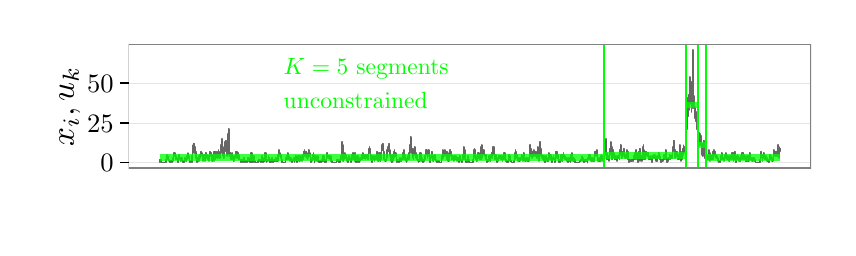
\begin{tikzpicture}[x=1pt,y=1pt]
\definecolor{fillColor}{RGB}{255,255,255}
\path[use as bounding box,fill=fillColor,fill opacity=0.00] (0,0) rectangle (289.08, 72.27);
\begin{scope}
\path[clip] (  0.00,  0.00) rectangle (289.08, 72.27);
\definecolor{drawColor}{RGB}{255,255,255}
\definecolor{fillColor}{RGB}{255,255,255}

\path[draw=drawColor,line width= 0.6pt,line join=round,line cap=round,fill=fillColor] (  0.00,  0.00) rectangle (289.08, 72.27);
\end{scope}
\begin{scope}
\path[clip] ( 36.46, 21.46) rectangle (283.08, 66.27);
\definecolor{fillColor}{RGB}{255,255,255}

\path[fill=fillColor] ( 36.46, 21.46) rectangle (283.08, 66.27);
\definecolor{drawColor}{gray}{0.90}

\path[draw=drawColor,line width= 0.2pt,line join=round] ( 36.46, 23.50) --
	(283.08, 23.50);

\path[draw=drawColor,line width= 0.2pt,line join=round] ( 36.46, 37.84) --
	(283.08, 37.84);

\path[draw=drawColor,line width= 0.2pt,line join=round] ( 36.46, 52.19) --
	(283.08, 52.19);
\definecolor{drawColor}{gray}{0.40}

\path[draw=drawColor,line width= 0.6pt,line join=round] ( 47.67, 24.07) --
	( 47.86, 24.07) --
	( 47.86, 23.50) --
	( 47.87, 23.50) --
	( 47.87, 24.07) --
	( 47.88, 24.07) --
	( 47.88, 24.65) --
	( 48.30, 24.65) --
	( 48.30, 24.07) --
	( 48.33, 24.07) --
	( 48.33, 23.50) --
	( 49.90, 23.50) --
	( 49.90, 24.07) --
	( 49.94, 24.07) --
	( 49.94, 24.65) --
	( 50.17, 24.65) --
	( 50.17, 25.22) --
	( 50.24, 25.22) --
	( 50.24, 25.80) --
	( 50.30, 25.80) --
	( 50.30, 26.37) --
	( 50.35, 26.37) --
	( 50.35, 25.80) --
	( 50.39, 25.80) --
	( 50.39, 25.22) --
	( 50.51, 25.22) --
	( 50.51, 25.80) --
	( 50.62, 25.80) --
	( 50.62, 25.22) --
	( 50.68, 25.22) --
	( 50.68, 25.80) --
	( 50.69, 25.80) --
	( 50.69, 25.22) --
	( 50.75, 25.22) --
	( 50.75, 24.65) --
	( 50.96, 24.65) --
	( 50.96, 24.07) --
	( 50.98, 24.07) --
	( 50.98, 24.65) --
	( 51.12, 24.65) --
	( 51.12, 24.07) --
	( 51.43, 24.07) --
	( 51.43, 23.50) --
	( 51.86, 23.50) --
	( 51.86, 24.07) --
	( 52.31, 24.07) --
	( 52.31, 23.50) --
	( 52.34, 23.50) --
	( 52.34, 24.07) --
	( 52.52, 24.07) --
	( 52.52, 24.65) --
	( 52.62, 24.65) --
	( 52.62, 25.22) --
	( 52.70, 25.22) --
	( 52.70, 25.80) --
	( 52.72, 25.80) --
	( 52.72, 26.37) --
	( 52.79, 26.37) --
	( 52.79, 25.80) --
	( 52.85, 25.80) --
	( 52.85, 26.37) --
	( 52.95, 26.37) --
	( 52.95, 26.94) --
	( 52.97, 26.94) --
	( 52.97, 26.37) --
	( 52.97, 26.37) --
	( 52.97, 26.94) --
	( 53.06, 26.94) --
	( 53.06, 26.37) --
	( 53.12, 26.37) --
	( 53.12, 26.94) --
	( 53.15, 26.94) --
	( 53.15, 26.37) --
	( 53.16, 26.37) --
	( 53.16, 25.80) --
	( 53.18, 25.80) --
	( 53.18, 26.37) --
	( 53.30, 26.37) --
	( 53.30, 25.80) --
	( 53.40, 25.80) --
	( 53.40, 25.22) --
	( 53.42, 25.22) --
	( 53.42, 24.65) --
	( 53.45, 24.65) --
	( 53.45, 25.22) --
	( 53.47, 25.22) --
	( 53.47, 25.80) --
	( 53.57, 25.80) --
	( 53.57, 25.22) --
	( 53.62, 25.22) --
	( 53.62, 24.65) --
	( 53.90, 24.65) --
	( 53.90, 25.22) --
	( 53.91, 25.22) --
	( 53.91, 24.65) --
	( 54.34, 24.65) --
	( 54.34, 23.50) --
	( 54.45, 23.50) --
	( 54.45, 24.07) --
	( 54.47, 24.07) --
	( 54.47, 24.65) --
	( 54.52, 24.65) --
	( 54.52, 25.22) --
	( 54.66, 25.22) --
	( 54.66, 25.80) --
	( 54.73, 25.80) --
	( 54.73, 26.37) --
	( 54.90, 26.37) --
	( 54.90, 25.80) --
	( 54.92, 25.80) --
	( 54.92, 25.22) --
	( 54.97, 25.22) --
	( 54.97, 24.65) --
	( 54.98, 24.65) --
	( 54.98, 25.22) --
	( 55.11, 25.22) --
	( 55.11, 24.65) --
	( 55.18, 24.65) --
	( 55.18, 24.07) --
	( 55.23, 24.07) --
	( 55.23, 24.65) --
	( 55.32, 24.65) --
	( 55.32, 25.22) --
	( 55.42, 25.22) --
	( 55.42, 24.65) --
	( 55.61, 24.65) --
	( 55.61, 25.22) --
	( 55.68, 25.22) --
	( 55.68, 24.65) --
	( 55.77, 24.65) --
	( 55.77, 24.07) --
	( 56.06, 24.07) --
	( 56.06, 23.50) --
	( 56.42, 23.50) --
	( 56.42, 24.07) --
	( 56.64, 24.07) --
	( 56.64, 24.65) --
	( 56.71, 24.65) --
	( 56.71, 25.22) --
	( 56.86, 25.22) --
	( 56.86, 24.65) --
	( 56.97, 24.65) --
	( 56.97, 25.22) --
	( 57.09, 25.22) --
	( 57.09, 24.65) --
	( 57.16, 24.65) --
	( 57.16, 24.07) --
	( 57.39, 24.07) --
	( 57.39, 24.65) --
	( 57.42, 24.65) --
	( 57.42, 24.07) --
	( 57.42, 24.07) --
	( 57.42, 24.65) --
	( 57.60, 24.65) --
	( 57.60, 25.80) --
	( 57.78, 25.80) --
	( 57.78, 26.37) --
	( 57.84, 26.37) --
	( 57.84, 25.80) --
	( 57.87, 25.80) --
	( 57.87, 25.22) --
	( 58.02, 25.22) --
	( 58.02, 26.37) --
	( 58.04, 26.37) --
	( 58.04, 26.94) --
	( 58.04, 26.94) --
	( 58.04, 25.80) --
	( 58.23, 25.80) --
	( 58.23, 25.22) --
	( 58.47, 25.22) --
	( 58.47, 24.07) --
	( 58.47, 24.07) --
	( 58.47, 23.50) --
	( 58.73, 23.50) --
	( 58.73, 24.07) --
	( 59.18, 24.07) --
	( 59.18, 23.50) --
	( 59.31, 23.50) --
	( 59.31, 24.07) --
	( 59.37, 24.07) --
	( 59.37, 24.65) --
	( 59.42, 24.65) --
	( 59.42, 25.80) --
	( 59.51, 25.80) --
	( 59.51, 26.94) --
	( 59.64, 26.94) --
	( 59.64, 27.52) --
	( 59.69, 27.52) --
	( 59.69, 28.09) --
	( 59.76, 28.09) --
	( 59.76, 27.52) --
	( 59.79, 27.52) --
	( 59.79, 29.24) --
	( 59.81, 29.24) --
	( 59.81, 29.81) --
	( 59.81, 29.81) --
	( 59.81, 29.24) --
	( 59.86, 29.24) --
	( 59.86, 30.39) --
	( 59.86, 30.39) --
	( 59.86, 29.24) --
	( 59.93, 29.24) --
	( 59.93, 29.81) --
	( 59.96, 29.81) --
	( 59.96, 28.66) --
	( 60.02, 28.66) --
	( 60.02, 29.24) --
	( 60.10, 29.24) --
	( 60.10, 28.66) --
	( 60.14, 28.66) --
	( 60.14, 28.09) --
	( 60.18, 28.09) --
	( 60.18, 29.81) --
	( 60.22, 29.81) --
	( 60.22, 30.39) --
	( 60.24, 30.39) --
	( 60.24, 29.81) --
	( 60.24, 29.81) --
	( 60.24, 28.66) --
	( 60.25, 28.66) --
	( 60.25, 28.09) --
	( 60.31, 28.09) --
	( 60.31, 26.94) --
	( 60.40, 26.94) --
	( 60.40, 27.52) --
	( 60.42, 27.52) --
	( 60.42, 28.09) --
	( 60.42, 28.09) --
	( 60.42, 28.66) --
	( 60.47, 28.66) --
	( 60.47, 28.09) --
	( 60.58, 28.09) --
	( 60.58, 28.66) --
	( 60.60, 28.66) --
	( 60.60, 29.24) --
	( 60.63, 29.24) --
	( 60.63, 27.52) --
	( 60.64, 27.52) --
	( 60.64, 28.09) --
	( 60.67, 28.09) --
	( 60.67, 27.52) --
	( 60.83, 27.52) --
	( 60.83, 26.94) --
	( 60.85, 26.94) --
	( 60.85, 26.37) --
	( 60.87, 26.37) --
	( 60.87, 25.22) --
	( 61.03, 25.22) --
	( 61.03, 24.07) --
	( 61.08, 24.07) --
	( 61.08, 23.50) --
	( 61.13, 23.50) --
	( 61.13, 24.07) --
	( 61.22, 24.07) --
	( 61.22, 24.65) --
	( 61.44, 24.65) --
	( 61.44, 25.22) --
	( 61.58, 25.22) --
	( 61.58, 24.65) --
	( 61.67, 24.65) --
	( 61.67, 24.07) --
	( 61.79, 24.07) --
	( 61.79, 24.65) --
	( 61.89, 24.65) --
	( 61.89, 24.07) --
	( 61.90, 24.07) --
	( 61.90, 24.65) --
	( 61.94, 24.65) --
	( 61.94, 25.22) --
	( 61.96, 25.22) --
	( 61.96, 25.80) --
	( 62.12, 25.80) --
	( 62.12, 26.37) --
	( 62.24, 26.37) --
	( 62.24, 25.80) --
	( 62.25, 25.80) --
	( 62.25, 26.37) --
	( 62.35, 26.37) --
	( 62.35, 25.80) --
	( 62.39, 25.80) --
	( 62.39, 25.22) --
	( 62.39, 25.22) --
	( 62.39, 26.37) --
	( 62.41, 26.37) --
	( 62.41, 25.80) --
	( 62.49, 25.80) --
	( 62.49, 26.37) --
	( 62.50, 26.37) --
	( 62.50, 26.94) --
	( 62.65, 26.94) --
	( 62.65, 27.52) --
	( 62.70, 27.52) --
	( 62.70, 26.94) --
	( 62.79, 26.94) --
	( 62.79, 27.52) --
	( 62.84, 27.52) --
	( 62.84, 26.37) --
	( 62.93, 26.37) --
	( 62.93, 26.94) --
	( 62.94, 26.94) --
	( 62.94, 26.37) --
	( 62.95, 26.37) --
	( 62.95, 25.80) --
	( 62.98, 25.80) --
	( 62.98, 26.94) --
	( 63.02, 26.94) --
	( 63.02, 26.37) --
	( 63.10, 26.37) --
	( 63.10, 25.80) --
	( 63.24, 25.80) --
	( 63.24, 25.22) --
	( 63.34, 25.22) --
	( 63.34, 25.80) --
	( 63.37, 25.80) --
	( 63.37, 25.22) --
	( 63.43, 25.22) --
	( 63.43, 24.07) --
	( 63.45, 24.07) --
	( 63.45, 24.65) --
	( 63.46, 24.65) --
	( 63.46, 25.22) --
	( 63.52, 25.22) --
	( 63.52, 25.80) --
	( 63.77, 25.80) --
	( 63.77, 26.37) --
	( 63.79, 26.37) --
	( 63.79, 25.80) --
	( 63.90, 25.80) --
	( 63.90, 25.22) --
	( 63.91, 25.22) --
	( 63.91, 24.65) --
	( 63.97, 24.65) --
	( 63.97, 24.07) --
	( 64.05, 24.07) --
	( 64.05, 24.65) --
	( 64.16, 24.65) --
	( 64.16, 25.22) --
	( 64.18, 25.22) --
	( 64.18, 25.80) --
	( 64.19, 25.80) --
	( 64.19, 26.37) --
	( 64.21, 26.37) --
	( 64.21, 25.80) --
	( 64.23, 25.80) --
	( 64.23, 26.37) --
	( 64.29, 26.37) --
	( 64.29, 26.94) --
	( 64.50, 26.94) --
	( 64.50, 26.37) --
	( 64.58, 26.37) --
	( 64.58, 26.94) --
	( 64.63, 26.94) --
	( 64.63, 26.37) --
	( 64.64, 26.37) --
	( 64.64, 25.80) --
	( 64.65, 25.80) --
	( 64.65, 26.37) --
	( 64.68, 26.37) --
	( 64.68, 25.80) --
	( 64.74, 25.80) --
	( 64.74, 25.22) --
	( 64.96, 25.22) --
	( 64.96, 25.80) --
	( 64.99, 25.80) --
	( 64.99, 26.37) --
	( 65.02, 26.37) --
	( 65.02, 25.80) --
	( 65.05, 25.80) --
	( 65.05, 25.22) --
	( 65.09, 25.22) --
	( 65.09, 24.65) --
	( 65.39, 24.65) --
	( 65.39, 25.22) --
	( 65.41, 25.22) --
	( 65.41, 24.65) --
	( 65.44, 24.65) --
	( 65.44, 24.07) --
	( 65.50, 24.07) --
	( 65.50, 24.65) --
	( 65.50, 24.65) --
	( 65.50, 25.22) --
	( 65.60, 25.22) --
	( 65.60, 25.80) --
	( 65.68, 25.80) --
	( 65.68, 26.37) --
	( 65.70, 26.37) --
	( 65.70, 26.94) --
	( 65.79, 26.94) --
	( 65.79, 27.52) --
	( 65.84, 27.52) --
	( 65.84, 26.94) --
	( 65.93, 26.94) --
	( 65.93, 27.52) --
	( 65.94, 27.52) --
	( 65.94, 26.94) --
	( 65.95, 26.94) --
	( 65.95, 26.37) --
	( 66.01, 26.37) --
	( 66.01, 25.80) --
	( 66.05, 25.80) --
	( 66.05, 26.37) --
	( 66.11, 26.37) --
	( 66.11, 26.94) --
	( 66.12, 26.94) --
	( 66.12, 26.37) --
	( 66.13, 26.37) --
	( 66.13, 26.94) --
	( 66.15, 26.94) --
	( 66.15, 26.37) --
	( 66.18, 26.37) --
	( 66.18, 26.94) --
	( 66.24, 26.94) --
	( 66.24, 26.37) --
	( 66.29, 26.37) --
	( 66.29, 26.94) --
	( 66.37, 26.94) --
	( 66.37, 26.37) --
	( 66.50, 26.37) --
	( 66.50, 25.80) --
	( 66.56, 25.80) --
	( 66.56, 25.22) --
	( 66.58, 25.22) --
	( 66.58, 24.65) --
	( 66.63, 24.65) --
	( 66.63, 24.07) --
	( 66.65, 24.07) --
	( 66.65, 24.65) --
	( 66.67, 24.65) --
	( 66.67, 24.07) --
	( 66.81, 24.07) --
	( 66.81, 24.65) --
	( 67.05, 24.65) --
	( 67.05, 25.22) --
	( 67.10, 25.22) --
	( 67.10, 24.65) --
	( 67.25, 24.65) --
	( 67.25, 24.07) --
	( 67.28, 24.07) --
	( 67.28, 25.22) --
	( 67.30, 25.22) --
	( 67.30, 25.80) --
	( 67.32, 25.80) --
	( 67.32, 26.37) --
	( 67.34, 26.37) --
	( 67.34, 26.94) --
	( 67.37, 26.94) --
	( 67.37, 27.52) --
	( 67.50, 27.52) --
	( 67.50, 26.94) --
	( 67.57, 26.94) --
	( 67.57, 27.52) --
	( 67.72, 27.52) --
	( 67.72, 26.37) --
	( 67.75, 26.37) --
	( 67.75, 25.80) --
	( 67.76, 25.80) --
	( 67.76, 25.22) --
	( 67.82, 25.22) --
	( 67.82, 24.65) --
	( 67.90, 24.65) --
	( 67.90, 25.22) --
	( 67.93, 25.22) --
	( 67.93, 26.37) --
	( 68.05, 26.37) --
	( 68.05, 26.94) --
	( 68.09, 26.94) --
	( 68.09, 27.52) --
	( 68.24, 27.52) --
	( 68.24, 26.94) --
	( 68.35, 26.94) --
	( 68.35, 26.37) --
	( 68.37, 26.37) --
	( 68.37, 25.22) --
	( 68.40, 25.22) --
	( 68.40, 25.80) --
	( 68.46, 25.80) --
	( 68.46, 25.22) --
	( 68.49, 25.22) --
	( 68.49, 25.80) --
	( 68.50, 25.80) --
	( 68.50, 25.22) --
	( 68.53, 25.22) --
	( 68.53, 25.80) --
	( 68.54, 25.80) --
	( 68.54, 25.22) --
	( 68.59, 25.22) --
	( 68.59, 25.80) --
	( 68.67, 25.80) --
	( 68.67, 26.37) --
	( 68.70, 26.37) --
	( 68.70, 26.94) --
	( 68.77, 26.94) --
	( 68.77, 27.52) --
	( 68.85, 27.52) --
	( 68.85, 26.94) --
	( 68.85, 26.94) --
	( 68.85, 27.52) --
	( 68.93, 27.52) --
	( 68.93, 26.94) --
	( 68.97, 26.94) --
	( 68.97, 27.52) --
	( 68.97, 27.52) --
	( 68.97, 28.09) --
	( 68.98, 28.09) --
	( 68.98, 27.52) --
	( 69.04, 27.52) --
	( 69.04, 26.94) --
	( 69.12, 26.94) --
	( 69.12, 26.37) --
	( 69.15, 26.37) --
	( 69.15, 25.80) --
	( 69.22, 25.80) --
	( 69.22, 25.22) --
	( 69.23, 25.22) --
	( 69.23, 25.80) --
	( 69.26, 25.80) --
	( 69.26, 26.94) --
	( 69.30, 26.94) --
	( 69.30, 26.37) --
	( 69.41, 26.37) --
	( 69.41, 25.80) --
	( 69.42, 25.80) --
	( 69.42, 25.22) --
	( 69.44, 25.22) --
	( 69.44, 25.80) --
	( 69.49, 25.80) --
	( 69.49, 26.37) --
	( 69.56, 26.37) --
	( 69.56, 26.94) --
	( 69.66, 26.94) --
	( 69.66, 27.52) --
	( 69.68, 27.52) --
	( 69.68, 26.94) --
	( 69.69, 26.94) --
	( 69.69, 27.52) --
	( 69.70, 27.52) --
	( 69.70, 28.09) --
	( 69.71, 28.09) --
	( 69.71, 27.52) --
	( 69.71, 27.52) --
	( 69.71, 26.94) --
	( 69.74, 26.94) --
	( 69.74, 27.52) --
	( 69.88, 27.52) --
	( 69.88, 28.09) --
	( 69.89, 28.09) --
	( 69.89, 27.52) --
	( 69.93, 27.52) --
	( 69.93, 28.09) --
	( 69.93, 28.09) --
	( 69.93, 27.52) --
	( 69.96, 27.52) --
	( 69.96, 29.24) --
	( 69.96, 29.24) --
	( 69.96, 29.81) --
	( 69.98, 29.81) --
	( 69.98, 29.24) --
	( 70.01, 29.24) --
	( 70.01, 29.81) --
	( 70.05, 29.81) --
	( 70.05, 30.39) --
	( 70.09, 30.39) --
	( 70.09, 30.96) --
	( 70.11, 30.96) --
	( 70.11, 30.39) --
	( 70.14, 30.39) --
	( 70.14, 29.81) --
	( 70.15, 29.81) --
	( 70.15, 29.24) --
	( 70.15, 29.24) --
	( 70.15, 29.81) --
	( 70.18, 29.81) --
	( 70.18, 30.39) --
	( 70.19, 30.39) --
	( 70.19, 29.81) --
	( 70.19, 29.81) --
	( 70.19, 30.96) --
	( 70.26, 30.96) --
	( 70.26, 31.53) --
	( 70.32, 31.53) --
	( 70.32, 32.11) --
	( 70.32, 32.11) --
	( 70.32, 31.53) --
	( 70.38, 31.53) --
	( 70.38, 30.96) --
	( 70.41, 30.96) --
	( 70.41, 29.24) --
	( 70.41, 29.24) --
	( 70.41, 28.09) --
	( 70.42, 28.09) --
	( 70.42, 28.66) --
	( 70.48, 28.66) --
	( 70.48, 29.24) --
	( 70.50, 29.24) --
	( 70.50, 28.66) --
	( 70.54, 28.66) --
	( 70.54, 28.09) --
	( 70.55, 28.09) --
	( 70.55, 27.52) --
	( 70.63, 27.52) --
	( 70.63, 26.94) --
	( 70.64, 26.94) --
	( 70.64, 25.80) --
	( 70.68, 25.80) --
	( 70.68, 26.37) --
	( 70.70, 26.37) --
	( 70.70, 25.22) --
	( 70.79, 25.22) --
	( 70.79, 25.80) --
	( 70.87, 25.80) --
	( 70.87, 26.37) --
	( 70.87, 26.37) --
	( 70.87, 25.80) --
	( 70.93, 25.80) --
	( 70.93, 25.22) --
	( 70.99, 25.22) --
	( 70.99, 26.37) --
	( 71.03, 26.37) --
	( 71.03, 26.94) --
	( 71.07, 26.94) --
	( 71.07, 27.52) --
	( 71.08, 27.52) --
	( 71.08, 26.94) --
	( 71.15, 26.94) --
	( 71.15, 27.52) --
	( 71.17, 27.52) --
	( 71.17, 28.09) --
	( 71.24, 28.09) --
	( 71.24, 27.52) --
	( 71.27, 27.52) --
	( 71.27, 28.09) --
	( 71.27, 28.09) --
	( 71.27, 28.66) --
	( 71.31, 28.66) --
	( 71.31, 29.24) --
	( 71.33, 29.24) --
	( 71.33, 28.66) --
	( 71.35, 28.66) --
	( 71.35, 29.24) --
	( 71.38, 29.24) --
	( 71.38, 29.81) --
	( 71.40, 29.81) --
	( 71.40, 30.39) --
	( 71.41, 30.39) --
	( 71.41, 30.96) --
	( 71.45, 30.96) --
	( 71.45, 31.53) --
	( 71.48, 31.53) --
	( 71.48, 30.96) --
	( 71.50, 30.96) --
	( 71.50, 31.53) --
	( 71.52, 31.53) --
	( 71.52, 30.96) --
	( 71.53, 30.96) --
	( 71.53, 30.39) --
	( 71.56, 30.39) --
	( 71.56, 30.96) --
	( 71.57, 30.96) --
	( 71.57, 31.53) --
	( 71.59, 31.53) --
	( 71.59, 30.96) --
	( 71.67, 30.96) --
	( 71.67, 31.53) --
	( 71.72, 31.53) --
	( 71.72, 30.96) --
	( 71.75, 30.96) --
	( 71.75, 30.39) --
	( 71.76, 30.39) --
	( 71.76, 30.96) --
	( 71.76, 30.96) --
	( 71.76, 30.39) --
	( 71.80, 30.39) --
	( 71.80, 30.96) --
	( 71.83, 30.96) --
	( 71.83, 30.39) --
	( 71.85, 30.39) --
	( 71.85, 29.81) --
	( 71.85, 29.81) --
	( 71.85, 29.24) --
	( 71.89, 29.24) --
	( 71.89, 28.66) --
	( 71.90, 28.66) --
	( 71.90, 28.09) --
	( 71.94, 28.09) --
	( 71.94, 27.52) --
	( 72.00, 27.52) --
	( 72.00, 26.94) --
	( 72.00, 26.94) --
	( 72.00, 27.52) --
	( 72.01, 27.52) --
	( 72.01, 26.94) --
	( 72.02, 26.94) --
	( 72.02, 26.37) --
	( 72.06, 26.37) --
	( 72.06, 25.80) --
	( 72.07, 25.80) --
	( 72.07, 26.37) --
	( 72.11, 26.37) --
	( 72.11, 26.94) --
	( 72.11, 26.94) --
	( 72.11, 26.37) --
	( 72.19, 26.37) --
	( 72.19, 26.94) --
	( 72.21, 26.94) --
	( 72.21, 26.37) --
	( 72.24, 26.37) --
	( 72.24, 25.80) --
	( 72.26, 25.80) --
	( 72.26, 26.37) --
	( 72.27, 26.37) --
	( 72.27, 27.52) --
	( 72.28, 27.52) --
	( 72.28, 28.09) --
	( 72.33, 28.09) --
	( 72.33, 28.66) --
	( 72.37, 28.66) --
	( 72.37, 29.24) --
	( 72.38, 29.24) --
	( 72.38, 29.81) --
	( 72.38, 29.81) --
	( 72.38, 30.39) --
	( 72.42, 30.39) --
	( 72.42, 30.96) --
	( 72.44, 30.96) --
	( 72.44, 31.53) --
	( 72.45, 31.53) --
	( 72.45, 30.96) --
	( 72.45, 30.96) --
	( 72.45, 31.53) --
	( 72.47, 31.53) --
	( 72.47, 33.25) --
	( 72.49, 33.25) --
	( 72.49, 33.83) --
	( 72.51, 33.83) --
	( 72.51, 33.25) --
	( 72.52, 33.25) --
	( 72.52, 33.83) --
	( 72.53, 33.83) --
	( 72.53, 34.40) --
	( 72.54, 34.40) --
	( 72.54, 34.98) --
	( 72.55, 34.98) --
	( 72.55, 35.55) --
	( 72.56, 35.55) --
	( 72.56, 34.98) --
	( 72.61, 34.98) --
	( 72.61, 35.55) --
	( 72.64, 35.55) --
	( 72.64, 34.98) --
	( 72.71, 34.98) --
	( 72.71, 34.40) --
	( 72.71, 34.40) --
	( 72.71, 33.83) --
	( 72.72, 33.83) --
	( 72.72, 33.25) --
	( 72.78, 33.25) --
	( 72.78, 32.68) --
	( 72.81, 32.68) --
	( 72.81, 32.11) --
	( 72.83, 32.11) --
	( 72.83, 31.53) --
	( 72.83, 31.53) --
	( 72.83, 30.96) --
	( 72.87, 30.96) --
	( 72.87, 30.39) --
	( 72.89, 30.39) --
	( 72.89, 29.81) --
	( 72.90, 29.81) --
	( 72.90, 29.24) --
	( 72.92, 29.24) --
	( 72.92, 27.52) --
	( 72.93, 27.52) --
	( 72.93, 28.09) --
	( 72.93, 28.09) --
	( 72.93, 26.94) --
	( 72.97, 26.94) --
	( 72.97, 26.37) --
	( 72.97, 26.37) --
	( 72.97, 25.80) --
	( 72.99, 25.80) --
	( 72.99, 26.37) --
	( 72.99, 26.37) --
	( 72.99, 26.94) --
	( 73.01, 26.94) --
	( 73.01, 26.37) --
	( 73.06, 26.37) --
	( 73.06, 25.80) --
	( 73.18, 25.80) --
	( 73.18, 26.94) --
	( 73.37, 26.94) --
	( 73.37, 26.37) --
	( 73.44, 26.37) --
	( 73.44, 24.65) --
	( 73.60, 24.65) --
	( 73.60, 25.80) --
	( 73.63, 25.80) --
	( 73.63, 24.65) --
	( 73.71, 24.65) --
	( 73.71, 25.22) --
	( 73.84, 25.22) --
	( 73.84, 25.80) --
	( 73.97, 25.80) --
	( 73.97, 26.37) --
	( 73.98, 26.37) --
	( 73.98, 26.94) --
	( 74.05, 26.94) --
	( 74.05, 25.80) --
	( 74.15, 25.80) --
	( 74.15, 25.22) --
	( 74.28, 25.22) --
	( 74.28, 24.65) --
	( 74.29, 24.65) --
	( 74.29, 25.22) --
	( 74.42, 25.22) --
	( 74.42, 24.65) --
	( 74.43, 24.65) --
	( 74.43, 24.07) --
	( 74.45, 24.07) --
	( 74.45, 24.65) --
	( 74.46, 24.65) --
	( 74.46, 25.22) --
	( 74.73, 25.22) --
	( 74.73, 25.80) --
	( 74.74, 25.80) --
	( 74.74, 25.22) --
	( 74.88, 25.22) --
	( 74.88, 25.80) --
	( 74.91, 25.80) --
	( 74.91, 25.22) --
	( 74.98, 25.22) --
	( 74.98, 25.80) --
	( 75.10, 25.80) --
	( 75.10, 26.37) --
	( 75.18, 26.37) --
	( 75.18, 25.80) --
	( 75.22, 25.80) --
	( 75.22, 26.37) --
	( 75.28, 26.37) --
	( 75.28, 27.52) --
	( 75.32, 27.52) --
	( 75.32, 26.94) --
	( 75.35, 26.94) --
	( 75.35, 26.37) --
	( 75.43, 26.37) --
	( 75.43, 25.80) --
	( 75.48, 25.80) --
	( 75.48, 26.37) --
	( 75.49, 26.37) --
	( 75.49, 26.94) --
	( 75.55, 26.94) --
	( 75.55, 26.37) --
	( 75.60, 26.37) --
	( 75.60, 26.94) --
	( 75.64, 26.94) --
	( 75.64, 27.52) --
	( 75.65, 27.52) --
	( 75.65, 26.94) --
	( 75.66, 26.94) --
	( 75.66, 26.37) --
	( 75.68, 26.37) --
	( 75.68, 25.80) --
	( 75.72, 25.80) --
	( 75.72, 25.22) --
	( 75.80, 25.22) --
	( 75.80, 25.80) --
	( 75.82, 25.80) --
	( 75.82, 26.37) --
	( 75.85, 26.37) --
	( 75.85, 25.80) --
	( 75.93, 25.80) --
	( 75.93, 25.22) --
	( 75.96, 25.22) --
	( 75.96, 25.80) --
	( 75.96, 25.80) --
	( 75.96, 26.37) --
	( 76.06, 26.37) --
	( 76.06, 26.94) --
	( 76.09, 26.94) --
	( 76.09, 26.37) --
	( 76.09, 26.37) --
	( 76.09, 26.94) --
	( 76.24, 26.94) --
	( 76.24, 26.37) --
	( 76.27, 26.37) --
	( 76.27, 25.80) --
	( 76.40, 25.80) --
	( 76.40, 24.65) --
	( 76.48, 24.65) --
	( 76.48, 25.22) --
	( 76.50, 25.22) --
	( 76.50, 24.65) --
	( 76.51, 24.65) --
	( 76.51, 25.22) --
	( 76.54, 25.22) --
	( 76.54, 24.65) --
	( 76.93, 24.65) --
	( 76.93, 24.07) --
	( 76.96, 24.07) --
	( 76.96, 23.50) --
	( 77.15, 23.50) --
	( 77.15, 24.07) --
	( 77.26, 24.07) --
	( 77.26, 24.65) --
	( 77.55, 24.65) --
	( 77.55, 24.07) --
	( 77.71, 24.07) --
	( 77.71, 23.50) --
	( 77.89, 23.50) --
	( 77.89, 24.07) --
	( 77.95, 24.07) --
	( 77.95, 24.65) --
	( 77.96, 24.65) --
	( 77.96, 25.22) --
	( 78.33, 25.22) --
	( 78.33, 24.65) --
	( 78.40, 24.65) --
	( 78.40, 24.07) --
	( 78.41, 24.07) --
	( 78.41, 23.50) --
	( 78.64, 23.50) --
	( 78.64, 24.07) --
	( 79.09, 24.07) --
	( 79.09, 23.50) --
	( 79.30, 23.50) --
	( 79.30, 24.07) --
	( 79.43, 24.07) --
	( 79.43, 24.65) --
	( 79.60, 24.65) --
	( 79.60, 25.22) --
	( 79.64, 25.22) --
	( 79.64, 24.65) --
	( 79.75, 24.65) --
	( 79.75, 24.07) --
	( 79.92, 24.07) --
	( 79.92, 24.65) --
	( 79.97, 24.65) --
	( 79.97, 25.22) --
	( 80.05, 25.22) --
	( 80.05, 24.65) --
	( 80.36, 24.65) --
	( 80.36, 24.07) --
	( 80.42, 24.07) --
	( 80.42, 23.50) --
	( 80.60, 23.50) --
	( 80.60, 25.22) --
	( 80.62, 25.22) --
	( 80.62, 26.94) --
	( 81.04, 26.94) --
	( 81.04, 25.22) --
	( 81.07, 25.22) --
	( 81.07, 24.65) --
	( 81.07, 24.65) --
	( 81.07, 23.50) --
	( 81.32, 23.50) --
	( 81.32, 24.07) --
	( 81.35, 24.07) --
	( 81.35, 24.65) --
	( 81.53, 24.65) --
	( 81.53, 25.22) --
	( 81.67, 25.22) --
	( 81.67, 25.80) --
	( 81.73, 25.80) --
	( 81.73, 25.22) --
	( 81.79, 25.22) --
	( 81.79, 24.65) --
	( 81.97, 24.65) --
	( 81.97, 24.07) --
	( 82.12, 24.07) --
	( 82.12, 23.50) --
	( 83.16, 23.50) --
	( 83.16, 24.07) --
	( 83.40, 24.07) --
	( 83.40, 24.65) --
	( 83.61, 24.65) --
	( 83.61, 24.07) --
	( 83.64, 24.07) --
	( 83.64, 24.65) --
	( 83.85, 24.65) --
	( 83.85, 24.07) --
	( 83.89, 24.07) --
	( 83.89, 24.65) --
	( 84.08, 24.65) --
	( 84.08, 24.07) --
	( 84.34, 24.07) --
	( 84.34, 23.50) --
	( 84.38, 23.50) --
	( 84.38, 24.07) --
	( 84.61, 24.07) --
	( 84.61, 24.65) --
	( 84.63, 24.65) --
	( 84.63, 25.22) --
	( 84.65, 25.22) --
	( 84.65, 25.80) --
	( 84.83, 25.80) --
	( 84.83, 25.22) --
	( 85.06, 25.22) --
	( 85.06, 24.65) --
	( 85.08, 24.65) --
	( 85.08, 24.07) --
	( 85.09, 24.07) --
	( 85.09, 23.50) --
	( 85.20, 23.50) --
	( 85.20, 24.07) --
	( 85.58, 24.07) --
	( 85.58, 24.65) --
	( 85.65, 24.65) --
	( 85.65, 24.07) --
	( 85.73, 24.07) --
	( 85.73, 24.65) --
	( 85.81, 24.65) --
	( 85.81, 25.22) --
	( 85.84, 25.22) --
	( 85.84, 26.37) --
	( 85.85, 26.37) --
	( 85.85, 26.94) --
	( 86.02, 26.94) --
	( 86.02, 26.37) --
	( 86.17, 26.37) --
	( 86.17, 25.80) --
	( 86.25, 25.80) --
	( 86.25, 25.22) --
	( 86.29, 25.22) --
	( 86.29, 24.07) --
	( 86.30, 24.07) --
	( 86.30, 23.50) --
	( 86.33, 23.50) --
	( 86.33, 24.07) --
	( 86.56, 24.07) --
	( 86.56, 24.65) --
	( 86.78, 24.65) --
	( 86.78, 24.07) --
	( 86.91, 24.07) --
	( 86.91, 24.65) --
	( 86.96, 24.65) --
	( 86.96, 25.80) --
	( 87.01, 25.80) --
	( 87.01, 25.22) --
	( 87.35, 25.22) --
	( 87.35, 24.65) --
	( 87.41, 24.65) --
	( 87.41, 23.50) --
	( 87.47, 23.50) --
	( 87.47, 24.07) --
	( 87.71, 24.07) --
	( 87.71, 24.65) --
	( 87.92, 24.65) --
	( 87.92, 23.50) --
	( 87.98, 23.50) --
	( 87.98, 24.07) --
	( 88.13, 24.07) --
	( 88.13, 24.65) --
	( 88.38, 24.65) --
	( 88.38, 25.22) --
	( 88.41, 25.22) --
	( 88.41, 24.65) --
	( 88.57, 24.65) --
	( 88.57, 23.50) --
	( 88.82, 23.50) --
	( 88.82, 24.07) --
	( 89.25, 24.07) --
	( 89.25, 24.65) --
	( 89.27, 24.65) --
	( 89.27, 24.07) --
	( 89.35, 24.07) --
	( 89.35, 24.65) --
	( 89.51, 24.65) --
	( 89.51, 25.22) --
	( 89.69, 25.22) --
	( 89.69, 24.65) --
	( 89.79, 24.65) --
	( 89.79, 24.07) --
	( 89.81, 24.07) --
	( 89.81, 24.65) --
	( 89.94, 24.65) --
	( 89.94, 24.07) --
	( 90.07, 24.07) --
	( 90.07, 24.65) --
	( 90.26, 24.65) --
	( 90.26, 24.07) --
	( 90.41, 24.07) --
	( 90.41, 24.65) --
	( 90.43, 24.65) --
	( 90.43, 25.22) --
	( 90.48, 25.22) --
	( 90.48, 26.37) --
	( 90.52, 26.37) --
	( 90.52, 25.80) --
	( 90.55, 25.80) --
	( 90.55, 26.37) --
	( 90.58, 26.37) --
	( 90.58, 26.94) --
	( 90.69, 26.94) --
	( 90.69, 27.52) --
	( 90.80, 27.52) --
	( 90.80, 28.09) --
	( 90.86, 28.09) --
	( 90.86, 27.52) --
	( 90.87, 27.52) --
	( 90.87, 28.09) --
	( 90.87, 28.09) --
	( 90.87, 27.52) --
	( 90.92, 27.52) --
	( 90.92, 26.37) --
	( 90.99, 26.37) --
	( 90.99, 26.94) --
	( 91.00, 26.94) --
	( 91.00, 26.37) --
	( 91.01, 26.37) --
	( 91.01, 26.94) --
	( 91.03, 26.94) --
	( 91.03, 26.37) --
	( 91.11, 26.37) --
	( 91.11, 26.94) --
	( 91.14, 26.94) --
	( 91.14, 26.37) --
	( 91.25, 26.37) --
	( 91.25, 25.80) --
	( 91.28, 25.80) --
	( 91.28, 26.37) --
	( 91.31, 26.37) --
	( 91.31, 25.80) --
	( 91.38, 25.80) --
	( 91.38, 26.37) --
	( 91.44, 26.37) --
	( 91.44, 25.80) --
	( 91.44, 25.80) --
	( 91.44, 25.22) --
	( 91.52, 25.22) --
	( 91.52, 25.80) --
	( 91.56, 25.80) --
	( 91.56, 25.22) --
	( 91.73, 25.22) --
	( 91.73, 24.65) --
	( 91.83, 24.65) --
	( 91.83, 24.07) --
	( 91.96, 24.07) --
	( 91.96, 23.50) --
	( 93.18, 23.50) --
	( 93.18, 24.07) --
	( 93.21, 24.07) --
	( 93.21, 24.65) --
	( 93.35, 24.65) --
	( 93.35, 25.22) --
	( 93.63, 25.22) --
	( 93.63, 24.65) --
	( 93.63, 24.65) --
	( 93.63, 25.22) --
	( 93.65, 25.22) --
	( 93.65, 25.80) --
	( 93.66, 25.80) --
	( 93.66, 25.22) --
	( 93.80, 25.22) --
	( 93.80, 24.65) --
	( 93.88, 24.65) --
	( 93.88, 25.22) --
	( 93.96, 25.22) --
	( 93.96, 25.80) --
	( 94.06, 25.80) --
	( 94.06, 26.94) --
	( 94.08, 26.94) --
	( 94.08, 26.37) --
	( 94.10, 26.37) --
	( 94.10, 25.80) --
	( 94.33, 25.80) --
	( 94.33, 25.22) --
	( 94.37, 25.22) --
	( 94.37, 25.80) --
	( 94.40, 25.80) --
	( 94.40, 25.22) --
	( 94.43, 25.22) --
	( 94.43, 25.80) --
	( 94.51, 25.80) --
	( 94.51, 24.65) --
	( 94.78, 24.65) --
	( 94.78, 25.22) --
	( 94.82, 25.22) --
	( 94.82, 24.65) --
	( 94.87, 24.65) --
	( 94.87, 24.07) --
	( 94.90, 24.07) --
	( 94.90, 24.65) --
	( 94.98, 24.65) --
	( 94.98, 25.22) --
	( 95.23, 25.22) --
	( 95.23, 24.65) --
	( 95.35, 24.65) --
	( 95.35, 24.07) --
	( 95.43, 24.07) --
	( 95.43, 23.50) --
	( 95.67, 23.50) --
	( 95.67, 24.07) --
	( 95.68, 24.07) --
	( 95.68, 24.65) --
	( 96.00, 24.65) --
	( 96.00, 25.22) --
	( 96.12, 25.22) --
	( 96.12, 24.07) --
	( 96.45, 24.07) --
	( 96.45, 23.50) --
	( 96.46, 23.50) --
	( 96.46, 24.07) --
	( 96.64, 24.07) --
	( 96.64, 24.65) --
	( 96.71, 24.65) --
	( 96.71, 25.22) --
	( 96.74, 25.22) --
	( 96.74, 25.80) --
	( 96.91, 25.80) --
	( 96.91, 25.22) --
	( 97.08, 25.22) --
	( 97.08, 24.65) --
	( 97.16, 24.65) --
	( 97.16, 24.07) --
	( 97.19, 24.07) --
	( 97.19, 23.50) --
	( 97.24, 23.50) --
	( 97.24, 24.07) --
	( 97.61, 24.07) --
	( 97.61, 24.65) --
	( 97.68, 24.65) --
	( 97.68, 25.22) --
	( 97.69, 25.22) --
	( 97.69, 24.65) --
	( 97.69, 24.65) --
	( 97.69, 25.22) --
	( 97.80, 25.22) --
	( 97.80, 25.80) --
	( 98.05, 25.80) --
	( 98.05, 25.22) --
	( 98.08, 25.22) --
	( 98.08, 25.80) --
	( 98.13, 25.80) --
	( 98.13, 25.22) --
	( 98.13, 25.22) --
	( 98.13, 24.65) --
	( 98.24, 24.65) --
	( 98.24, 24.07) --
	( 98.37, 24.07) --
	( 98.37, 24.65) --
	( 98.45, 24.65) --
	( 98.45, 25.22) --
	( 98.52, 25.22) --
	( 98.52, 24.65) --
	( 98.58, 24.65) --
	( 98.58, 25.22) --
	( 98.67, 25.22) --
	( 98.67, 25.80) --
	( 98.81, 25.80) --
	( 98.81, 25.22) --
	( 98.83, 25.22) --
	( 98.83, 25.80) --
	( 98.90, 25.80) --
	( 98.90, 25.22) --
	( 99.03, 25.22) --
	( 99.03, 24.65) --
	( 99.12, 24.65) --
	( 99.12, 24.07) --
	( 99.14, 24.07) --
	( 99.14, 24.65) --
	( 99.17, 24.65) --
	( 99.17, 25.22) --
	( 99.28, 25.22) --
	( 99.28, 24.65) --
	( 99.33, 24.65) --
	( 99.33, 25.22) --
	( 99.41, 25.22) --
	( 99.41, 24.65) --
	( 99.43, 24.65) --
	( 99.43, 25.22) --
	( 99.54, 25.22) --
	( 99.54, 25.80) --
	( 99.58, 25.80) --
	( 99.58, 26.37) --
	( 99.64, 26.37) --
	( 99.64, 26.94) --
	( 99.72, 26.94) --
	( 99.72, 27.52) --
	( 99.78, 27.52) --
	( 99.78, 26.94) --
	( 99.87, 26.94) --
	( 99.87, 26.37) --
	( 99.91, 26.37) --
	( 99.91, 26.94) --
	( 99.92, 26.94) --
	( 99.92, 27.52) --
	( 99.98, 27.52) --
	( 99.98, 28.09) --
	( 99.99, 28.09) --
	( 99.99, 27.52) --
	(100.02, 27.52) --
	(100.02, 26.94) --
	(100.05, 26.94) --
	(100.05, 27.52) --
	(100.07, 27.52) --
	(100.07, 26.37) --
	(100.17, 26.37) --
	(100.17, 25.80) --
	(100.17, 25.80) --
	(100.17, 26.37) --
	(100.33, 26.37) --
	(100.33, 26.94) --
	(100.36, 26.94) --
	(100.36, 26.37) --
	(100.37, 26.37) --
	(100.37, 25.80) --
	(100.37, 25.80) --
	(100.37, 26.37) --
	(100.40, 26.37) --
	(100.40, 26.94) --
	(100.42, 26.94) --
	(100.42, 27.52) --
	(100.43, 27.52) --
	(100.43, 26.94) --
	(100.46, 26.94) --
	(100.46, 27.52) --
	(100.50, 27.52) --
	(100.50, 26.94) --
	(100.60, 26.94) --
	(100.60, 27.52) --
	(100.62, 27.52) --
	(100.62, 26.94) --
	(100.70, 26.94) --
	(100.70, 27.52) --
	(100.78, 27.52) --
	(100.78, 26.94) --
	(100.82, 26.94) --
	(100.82, 26.37) --
	(100.85, 26.37) --
	(100.85, 25.80) --
	(100.86, 25.80) --
	(100.86, 26.37) --
	(100.91, 26.37) --
	(100.91, 25.80) --
	(101.04, 25.80) --
	(101.04, 25.22) --
	(101.06, 25.22) --
	(101.06, 24.65) --
	(101.09, 24.65) --
	(101.09, 25.22) --
	(101.09, 25.22) --
	(101.09, 25.80) --
	(101.30, 25.80) --
	(101.30, 25.22) --
	(101.38, 25.22) --
	(101.38, 25.80) --
	(101.44, 25.80) --
	(101.44, 26.37) --
	(101.46, 26.37) --
	(101.46, 26.94) --
	(101.52, 26.94) --
	(101.52, 28.09) --
	(101.54, 28.09) --
	(101.54, 27.52) --
	(101.54, 27.52) --
	(101.54, 26.94) --
	(101.58, 26.94) --
	(101.58, 27.52) --
	(101.60, 27.52) --
	(101.60, 26.94) --
	(101.69, 26.94) --
	(101.69, 27.52) --
	(101.83, 27.52) --
	(101.83, 26.94) --
	(101.88, 26.94) --
	(101.88, 26.37) --
	(101.91, 26.37) --
	(101.91, 25.80) --
	(101.93, 25.80) --
	(101.93, 26.94) --
	(101.96, 26.94) --
	(101.96, 26.37) --
	(101.97, 26.37) --
	(101.97, 25.80) --
	(101.97, 25.80) --
	(101.97, 26.37) --
	(102.02, 26.37) --
	(102.02, 25.80) --
	(102.14, 25.80) --
	(102.14, 25.22) --
	(102.38, 25.22) --
	(102.38, 24.07) --
	(102.42, 24.07) --
	(102.42, 23.50) --
	(102.48, 23.50) --
	(102.48, 24.07) --
	(102.71, 24.07) --
	(102.71, 24.65) --
	(102.87, 24.65) --
	(102.87, 25.22) --
	(102.93, 25.22) --
	(102.93, 24.65) --
	(103.11, 24.65) --
	(103.11, 25.80) --
	(103.16, 25.80) --
	(103.16, 25.22) --
	(103.17, 25.22) --
	(103.17, 26.37) --
	(103.24, 26.37) --
	(103.24, 26.94) --
	(103.32, 26.94) --
	(103.32, 26.37) --
	(103.34, 26.37) --
	(103.34, 25.80) --
	(103.38, 25.80) --
	(103.38, 26.37) --
	(103.56, 26.37) --
	(103.56, 25.80) --
	(103.61, 25.80) --
	(103.61, 25.22) --
	(103.61, 25.22) --
	(103.61, 24.65) --
	(103.69, 24.65) --
	(103.69, 23.50) --
	(103.69, 23.50) --
	(103.69, 24.07) --
	(103.86, 24.07) --
	(103.86, 24.65) --
	(103.99, 24.65) --
	(103.99, 25.22) --
	(104.03, 25.22) --
	(104.03, 25.80) --
	(104.14, 25.80) --
	(104.14, 25.22) --
	(104.31, 25.22) --
	(104.31, 24.65) --
	(104.43, 24.65) --
	(104.43, 24.07) --
	(104.47, 24.07) --
	(104.47, 24.65) --
	(104.50, 24.65) --
	(104.50, 25.22) --
	(104.72, 25.22) --
	(104.72, 25.80) --
	(104.91, 25.80) --
	(104.91, 25.22) --
	(104.92, 25.22) --
	(104.92, 24.65) --
	(104.95, 24.65) --
	(104.95, 24.07) --
	(105.16, 24.07) --
	(105.16, 23.50) --
	(105.18, 23.50) --
	(105.18, 24.07) --
	(105.63, 24.07) --
	(105.63, 23.50) --
	(105.97, 23.50) --
	(105.97, 24.07) --
	(106.16, 24.07) --
	(106.16, 24.65) --
	(106.29, 24.65) --
	(106.29, 24.07) --
	(106.56, 24.07) --
	(106.56, 24.65) --
	(106.60, 24.65) --
	(106.60, 24.07) --
	(106.61, 24.07) --
	(106.61, 24.65) --
	(106.64, 24.65) --
	(106.64, 25.22) --
	(106.78, 25.22) --
	(106.78, 25.80) --
	(107.01, 25.80) --
	(107.01, 25.22) --
	(107.06, 25.22) --
	(107.06, 24.65) --
	(107.09, 24.65) --
	(107.09, 24.07) --
	(107.23, 24.07) --
	(107.23, 23.50) --
	(107.68, 23.50) --
	(107.68, 24.07) --
	(107.84, 24.07) --
	(107.84, 24.65) --
	(107.93, 24.65) --
	(107.93, 25.22) --
	(107.99, 25.22) --
	(107.99, 25.80) --
	(108.05, 25.80) --
	(108.05, 26.37) --
	(108.13, 26.37) --
	(108.13, 25.80) --
	(108.25, 25.80) --
	(108.25, 26.37) --
	(108.27, 26.37) --
	(108.27, 26.94) --
	(108.29, 26.94) --
	(108.29, 26.37) --
	(108.38, 26.37) --
	(108.38, 25.80) --
	(108.44, 25.80) --
	(108.44, 25.22) --
	(108.48, 25.22) --
	(108.48, 25.80) --
	(108.50, 25.80) --
	(108.50, 25.22) --
	(108.61, 25.22) --
	(108.61, 25.80) --
	(108.69, 25.80) --
	(108.69, 25.22) --
	(108.84, 25.22) --
	(108.84, 25.80) --
	(108.93, 25.80) --
	(108.93, 25.22) --
	(108.93, 25.22) --
	(108.93, 25.80) --
	(109.06, 25.80) --
	(109.06, 25.22) --
	(109.16, 25.22) --
	(109.16, 24.65) --
	(109.17, 24.65) --
	(109.17, 25.22) --
	(109.28, 25.22) --
	(109.28, 24.65) --
	(109.38, 24.65) --
	(109.38, 24.07) --
	(109.41, 24.07) --
	(109.41, 24.65) --
	(109.59, 24.65) --
	(109.59, 25.22) --
	(109.59, 25.22) --
	(109.59, 25.80) --
	(109.62, 25.80) --
	(109.62, 25.22) --
	(109.69, 25.22) --
	(109.69, 24.65) --
	(109.77, 24.65) --
	(109.77, 24.07) --
	(109.87, 24.07) --
	(109.87, 23.50) --
	(111.59, 23.50) --
	(111.59, 24.07) --
	(111.86, 24.07) --
	(111.86, 24.65) --
	(112.04, 24.65) --
	(112.04, 24.07) --
	(112.30, 24.07) --
	(112.30, 23.50) --
	(112.92, 23.50) --
	(112.92, 24.07) --
	(112.96, 24.07) --
	(112.96, 24.65) --
	(113.31, 24.65) --
	(113.31, 25.22) --
	(113.33, 25.22) --
	(113.33, 25.80) --
	(113.36, 25.80) --
	(113.36, 25.22) --
	(113.40, 25.22) --
	(113.40, 26.94) --
	(113.41, 26.94) --
	(113.41, 26.37) --
	(113.42, 26.37) --
	(113.42, 28.09) --
	(113.45, 28.09) --
	(113.45, 28.66) --
	(113.49, 28.66) --
	(113.49, 29.24) --
	(113.50, 29.24) --
	(113.50, 29.81) --
	(113.57, 29.81) --
	(113.57, 30.39) --
	(113.59, 30.39) --
	(113.59, 30.96) --
	(113.76, 30.96) --
	(113.76, 30.39) --
	(113.78, 30.39) --
	(113.78, 29.81) --
	(113.84, 29.81) --
	(113.84, 29.24) --
	(113.85, 29.24) --
	(113.85, 28.09) --
	(113.87, 28.09) --
	(113.87, 26.37) --
	(113.89, 26.37) --
	(113.89, 26.94) --
	(113.90, 26.94) --
	(113.90, 26.37) --
	(113.94, 26.37) --
	(113.94, 25.80) --
	(113.95, 25.80) --
	(113.95, 25.22) --
	(114.02, 25.22) --
	(114.02, 24.65) --
	(114.04, 24.65) --
	(114.04, 24.07) --
	(114.13, 24.07) --
	(114.13, 24.65) --
	(114.28, 24.65) --
	(114.28, 25.22) --
	(114.29, 25.22) --
	(114.29, 25.80) --
	(114.33, 25.80) --
	(114.33, 25.22) --
	(114.34, 25.22) --
	(114.34, 24.65) --
	(114.42, 24.65) --
	(114.42, 25.22) --
	(114.57, 25.22) --
	(114.57, 25.80) --
	(114.63, 25.80) --
	(114.63, 26.37) --
	(114.66, 26.37) --
	(114.66, 26.94) --
	(114.72, 26.94) --
	(114.72, 26.37) --
	(114.72, 26.37) --
	(114.72, 25.22) --
	(114.74, 25.22) --
	(114.74, 25.80) --
	(114.83, 25.80) --
	(114.83, 26.37) --
	(114.86, 26.37) --
	(114.86, 25.80) --
	(114.91, 25.80) --
	(114.91, 26.37) --
	(115.08, 26.37) --
	(115.08, 25.80) --
	(115.10, 25.80) --
	(115.10, 25.22) --
	(115.13, 25.22) --
	(115.13, 25.80) --
	(115.19, 25.80) --
	(115.19, 25.22) --
	(115.28, 25.22) --
	(115.28, 24.65) --
	(115.35, 24.65) --
	(115.35, 24.07) --
	(115.57, 24.07) --
	(115.57, 23.50) --
	(115.77, 23.50) --
	(115.77, 24.07) --
	(115.82, 24.07) --
	(115.82, 24.65) --
	(116.01, 24.65) --
	(116.01, 25.22) --
	(116.20, 25.22) --
	(116.20, 25.80) --
	(116.22, 25.80) --
	(116.22, 25.22) --
	(116.27, 25.22) --
	(116.27, 24.65) --
	(116.37, 24.65) --
	(116.37, 25.22) --
	(116.46, 25.22) --
	(116.46, 24.65) --
	(116.64, 24.65) --
	(116.64, 24.07) --
	(116.81, 24.07) --
	(116.81, 23.50) --
	(116.91, 23.50) --
	(116.91, 24.07) --
	(116.94, 24.07) --
	(116.94, 24.65) --
	(117.04, 24.65) --
	(117.04, 25.22) --
	(117.07, 25.22) --
	(117.07, 25.80) --
	(117.31, 25.80) --
	(117.31, 26.37) --
	(117.36, 26.37) --
	(117.36, 25.80) --
	(117.39, 25.80) --
	(117.39, 25.22) --
	(117.47, 25.22) --
	(117.47, 25.80) --
	(117.49, 25.80) --
	(117.49, 25.22) --
	(117.52, 25.22) --
	(117.52, 24.65) --
	(117.55, 24.65) --
	(117.55, 25.22) --
	(117.58, 25.22) --
	(117.58, 25.80) --
	(117.58, 25.80) --
	(117.58, 26.37) --
	(117.60, 26.37) --
	(117.60, 26.94) --
	(117.76, 26.94) --
	(117.76, 26.37) --
	(117.82, 26.37) --
	(117.82, 25.80) --
	(117.96, 25.80) --
	(117.96, 26.37) --
	(118.00, 26.37) --
	(118.00, 25.80) --
	(118.02, 25.80) --
	(118.02, 25.22) --
	(118.03, 25.22) --
	(118.03, 24.65) --
	(118.05, 24.65) --
	(118.05, 24.07) --
	(118.08, 24.07) --
	(118.08, 24.65) --
	(118.09, 24.65) --
	(118.09, 25.22) --
	(118.15, 25.22) --
	(118.15, 25.80) --
	(118.20, 25.80) --
	(118.20, 26.37) --
	(118.30, 26.37) --
	(118.30, 26.94) --
	(118.41, 26.94) --
	(118.41, 26.37) --
	(118.49, 26.37) --
	(118.49, 25.80) --
	(118.53, 25.80) --
	(118.53, 25.22) --
	(118.59, 25.22) --
	(118.59, 24.65) --
	(118.64, 24.65) --
	(118.64, 24.07) --
	(118.75, 24.07) --
	(118.75, 23.50) --
	(118.98, 23.50) --
	(118.98, 24.07) --
	(119.17, 24.07) --
	(119.17, 24.65) --
	(119.38, 24.65) --
	(119.38, 25.22) --
	(119.38, 25.22) --
	(119.38, 25.80) --
	(119.42, 25.80) --
	(119.42, 25.22) --
	(119.62, 25.22) --
	(119.62, 24.65) --
	(119.82, 24.65) --
	(119.82, 24.07) --
	(119.83, 24.07) --
	(119.83, 23.50) --
	(119.86, 23.50) --
	(119.86, 24.07) --
	(120.08, 24.07) --
	(120.08, 24.65) --
	(120.29, 24.65) --
	(120.29, 25.22) --
	(120.31, 25.22) --
	(120.31, 24.65) --
	(120.46, 24.65) --
	(120.46, 25.22) --
	(120.53, 25.22) --
	(120.53, 24.65) --
	(120.57, 24.65) --
	(120.57, 25.22) --
	(120.74, 25.22) --
	(120.74, 24.65) --
	(120.84, 24.65) --
	(120.84, 25.22) --
	(120.85, 25.22) --
	(120.85, 25.80) --
	(120.87, 25.80) --
	(120.87, 26.37) --
	(120.91, 26.37) --
	(120.91, 25.80) --
	(121.02, 25.80) --
	(121.02, 25.22) --
	(121.25, 25.22) --
	(121.25, 25.80) --
	(121.27, 25.80) --
	(121.27, 26.94) --
	(121.28, 26.94) --
	(121.28, 26.37) --
	(121.30, 26.37) --
	(121.30, 25.80) --
	(121.32, 25.80) --
	(121.32, 25.22) --
	(121.48, 25.22) --
	(121.48, 25.80) --
	(121.50, 25.80) --
	(121.50, 25.22) --
	(121.54, 25.22) --
	(121.54, 25.80) --
	(121.67, 25.80) --
	(121.67, 26.37) --
	(121.72, 26.37) --
	(121.72, 25.22) --
	(121.88, 25.22) --
	(121.88, 25.80) --
	(121.92, 25.80) --
	(121.92, 25.22) --
	(121.96, 25.22) --
	(121.96, 25.80) --
	(121.99, 25.80) --
	(121.99, 25.22) --
	(122.12, 25.22) --
	(122.12, 24.65) --
	(122.13, 24.65) --
	(122.13, 25.22) --
	(122.20, 25.22) --
	(122.20, 25.80) --
	(122.26, 25.80) --
	(122.26, 26.37) --
	(122.32, 26.37) --
	(122.32, 25.80) --
	(122.35, 25.80) --
	(122.35, 26.37) --
	(122.41, 26.37) --
	(122.41, 25.80) --
	(122.47, 25.80) --
	(122.47, 26.37) --
	(122.57, 26.37) --
	(122.57, 25.80) --
	(122.65, 25.80) --
	(122.65, 25.22) --
	(122.67, 25.22) --
	(122.67, 25.80) --
	(122.71, 25.80) --
	(122.71, 26.37) --
	(122.71, 26.37) --
	(122.71, 25.80) --
	(122.80, 25.80) --
	(122.80, 25.22) --
	(122.91, 25.22) --
	(122.91, 24.65) --
	(123.02, 24.65) --
	(123.02, 25.22) --
	(123.10, 25.22) --
	(123.10, 25.80) --
	(123.12, 25.80) --
	(123.12, 25.22) --
	(123.13, 25.22) --
	(123.13, 25.80) --
	(123.15, 25.80) --
	(123.15, 26.94) --
	(123.15, 26.94) --
	(123.15, 26.37) --
	(123.18, 26.37) --
	(123.18, 26.94) --
	(123.29, 26.94) --
	(123.29, 27.52) --
	(123.39, 27.52) --
	(123.39, 28.09) --
	(123.44, 28.09) --
	(123.44, 28.66) --
	(123.47, 28.66) --
	(123.47, 28.09) --
	(123.49, 28.09) --
	(123.49, 28.66) --
	(123.54, 28.66) --
	(123.54, 29.24) --
	(123.54, 29.24) --
	(123.54, 28.66) --
	(123.58, 28.66) --
	(123.58, 28.09) --
	(123.59, 28.09) --
	(123.59, 28.66) --
	(123.60, 28.66) --
	(123.60, 28.09) --
	(123.60, 28.09) --
	(123.60, 27.52) --
	(123.63, 27.52) --
	(123.63, 26.94) --
	(123.64, 26.94) --
	(123.64, 27.52) --
	(123.74, 27.52) --
	(123.74, 28.09) --
	(123.74, 28.09) --
	(123.74, 27.52) --
	(123.84, 27.52) --
	(123.84, 26.94) --
	(123.89, 26.94) --
	(123.89, 26.37) --
	(123.93, 26.37) --
	(123.93, 26.94) --
	(123.93, 26.94) --
	(123.93, 26.37) --
	(123.99, 26.37) --
	(123.99, 25.80) --
	(124.04, 25.80) --
	(124.04, 25.22) --
	(124.09, 25.22) --
	(124.09, 24.65) --
	(124.19, 24.65) --
	(124.19, 24.07) --
	(124.38, 24.07) --
	(124.38, 23.50) --
	(124.41, 23.50) --
	(124.41, 24.07) --
	(124.59, 24.07) --
	(124.59, 24.65) --
	(124.67, 24.65) --
	(124.67, 25.22) --
	(124.71, 25.22) --
	(124.71, 25.80) --
	(124.82, 25.80) --
	(124.82, 25.22) --
	(124.93, 25.22) --
	(124.93, 25.80) --
	(125.04, 25.80) --
	(125.04, 25.22) --
	(125.05, 25.22) --
	(125.05, 25.80) --
	(125.10, 25.80) --
	(125.10, 25.22) --
	(125.16, 25.22) --
	(125.16, 24.65) --
	(125.37, 24.65) --
	(125.37, 24.07) --
	(125.38, 24.07) --
	(125.38, 24.65) --
	(125.43, 24.65) --
	(125.43, 25.22) --
	(125.50, 25.22) --
	(125.50, 24.65) --
	(125.52, 24.65) --
	(125.52, 25.22) --
	(125.81, 25.22) --
	(125.81, 25.80) --
	(125.83, 25.80) --
	(125.83, 25.22) --
	(125.88, 25.22) --
	(125.88, 24.65) --
	(125.89, 24.65) --
	(125.89, 25.22) --
	(125.96, 25.22) --
	(125.96, 24.65) --
	(125.97, 24.65) --
	(125.97, 25.22) --
	(126.01, 25.22) --
	(126.01, 25.80) --
	(126.04, 25.80) --
	(126.04, 26.37) --
	(126.20, 26.37) --
	(126.20, 26.94) --
	(126.23, 26.94) --
	(126.23, 27.52) --
	(126.26, 27.52) --
	(126.26, 26.94) --
	(126.33, 26.94) --
	(126.33, 26.37) --
	(126.35, 26.37) --
	(126.35, 25.80) --
	(126.42, 25.80) --
	(126.42, 25.22) --
	(126.46, 25.22) --
	(126.46, 24.65) --
	(126.49, 24.65) --
	(126.49, 24.07) --
	(126.56, 24.07) --
	(126.56, 24.65) --
	(126.65, 24.65) --
	(126.65, 25.22) --
	(126.68, 25.22) --
	(126.68, 24.65) --
	(126.80, 24.65) --
	(126.80, 24.07) --
	(126.81, 24.07) --
	(126.81, 24.65) --
	(126.88, 24.65) --
	(126.88, 25.22) --
	(126.89, 25.22) --
	(126.89, 25.80) --
	(126.94, 25.80) --
	(126.94, 26.37) --
	(126.97, 26.37) --
	(126.97, 26.94) --
	(127.10, 26.94) --
	(127.10, 26.37) --
	(127.24, 26.37) --
	(127.24, 26.94) --
	(127.26, 26.94) --
	(127.26, 26.37) --
	(127.32, 26.37) --
	(127.32, 25.80) --
	(127.33, 25.80) --
	(127.33, 25.22) --
	(127.39, 25.22) --
	(127.39, 24.65) --
	(127.42, 24.65) --
	(127.42, 24.07) --
	(127.46, 24.07) --
	(127.46, 24.65) --
	(127.57, 24.65) --
	(127.57, 25.22) --
	(127.65, 25.22) --
	(127.65, 25.80) --
	(127.69, 25.80) --
	(127.69, 25.22) --
	(127.78, 25.22) --
	(127.78, 26.94) --
	(127.80, 26.94) --
	(127.80, 27.52) --
	(127.84, 27.52) --
	(127.84, 28.09) --
	(127.85, 28.09) --
	(127.85, 28.66) --
	(127.91, 28.66) --
	(127.91, 28.09) --
	(127.95, 28.09) --
	(127.95, 28.66) --
	(128.05, 28.66) --
	(128.05, 29.24) --
	(128.15, 29.24) --
	(128.15, 29.81) --
	(128.21, 29.81) --
	(128.21, 30.39) --
	(128.23, 30.39) --
	(128.23, 28.66) --
	(128.25, 28.66) --
	(128.25, 28.09) --
	(128.28, 28.09) --
	(128.28, 29.24) --
	(128.28, 29.24) --
	(128.28, 28.66) --
	(128.28, 28.66) --
	(128.28, 29.24) --
	(128.30, 29.24) --
	(128.30, 28.66) --
	(128.33, 28.66) --
	(128.33, 29.81) --
	(128.36, 29.81) --
	(128.36, 30.39) --
	(128.46, 30.39) --
	(128.46, 29.81) --
	(128.49, 29.81) --
	(128.49, 29.24) --
	(128.55, 29.24) --
	(128.55, 28.66) --
	(128.58, 28.66) --
	(128.58, 28.09) --
	(128.60, 28.09) --
	(128.60, 27.52) --
	(128.65, 27.52) --
	(128.65, 26.94) --
	(128.69, 26.94) --
	(128.69, 27.52) --
	(128.72, 27.52) --
	(128.72, 25.80) --
	(128.78, 25.80) --
	(128.78, 25.22) --
	(128.80, 25.22) --
	(128.80, 24.65) --
	(129.00, 24.65) --
	(129.00, 24.07) --
	(129.13, 24.07) --
	(129.13, 24.65) --
	(129.14, 24.65) --
	(129.14, 24.07) --
	(129.49, 24.07) --
	(129.49, 24.65) --
	(129.53, 24.65) --
	(129.53, 24.07) --
	(129.58, 24.07) --
	(129.58, 24.65) --
	(129.72, 24.65) --
	(129.72, 25.22) --
	(129.78, 25.22) --
	(129.78, 25.80) --
	(129.83, 25.80) --
	(129.83, 26.37) --
	(129.91, 26.37) --
	(129.91, 28.09) --
	(129.92, 28.09) --
	(129.92, 27.52) --
	(129.96, 27.52) --
	(129.96, 28.09) --
	(130.02, 28.09) --
	(130.02, 27.52) --
	(130.10, 27.52) --
	(130.10, 28.09) --
	(130.15, 28.09) --
	(130.15, 28.66) --
	(130.17, 28.66) --
	(130.17, 28.09) --
	(130.22, 28.09) --
	(130.22, 27.52) --
	(130.25, 27.52) --
	(130.25, 29.24) --
	(130.27, 29.24) --
	(130.27, 28.66) --
	(130.32, 28.66) --
	(130.32, 29.24) --
	(130.36, 29.24) --
	(130.36, 27.52) --
	(130.36, 27.52) --
	(130.36, 29.81) --
	(130.41, 29.81) --
	(130.41, 29.24) --
	(130.49, 29.24) --
	(130.49, 29.81) --
	(130.50, 29.81) --
	(130.50, 30.39) --
	(130.55, 30.39) --
	(130.55, 29.81) --
	(130.59, 29.81) --
	(130.59, 29.24) --
	(130.68, 29.24) --
	(130.68, 29.81) --
	(130.70, 29.81) --
	(130.70, 28.09) --
	(130.77, 28.09) --
	(130.77, 27.52) --
	(130.79, 27.52) --
	(130.79, 28.09) --
	(130.81, 28.09) --
	(130.81, 25.80) --
	(130.83, 25.80) --
	(130.83, 26.37) --
	(130.84, 26.37) --
	(130.84, 26.94) --
	(130.93, 26.94) --
	(130.93, 26.37) --
	(130.95, 26.37) --
	(130.95, 25.80) --
	(130.98, 25.80) --
	(130.98, 26.37) --
	(131.13, 26.37) --
	(131.13, 25.80) --
	(131.23, 25.80) --
	(131.23, 25.22) --
	(131.27, 25.22) --
	(131.27, 24.65) --
	(131.29, 24.65) --
	(131.29, 24.07) --
	(131.43, 24.07) --
	(131.43, 23.50) --
	(131.58, 23.50) --
	(131.58, 24.07) --
	(131.61, 24.07) --
	(131.61, 25.22) --
	(131.64, 25.22) --
	(131.64, 25.80) --
	(131.75, 25.80) --
	(131.75, 26.37) --
	(132.02, 26.37) --
	(132.02, 25.80) --
	(132.05, 25.80) --
	(132.05, 25.22) --
	(132.06, 25.22) --
	(132.06, 24.65) --
	(132.08, 24.65) --
	(132.08, 24.07) --
	(132.09, 24.07) --
	(132.09, 24.65) --
	(132.15, 24.65) --
	(132.15, 25.22) --
	(132.16, 25.22) --
	(132.16, 25.80) --
	(132.20, 25.80) --
	(132.20, 25.22) --
	(132.27, 25.22) --
	(132.27, 25.80) --
	(132.32, 25.80) --
	(132.32, 26.37) --
	(132.43, 26.37) --
	(132.43, 26.94) --
	(132.46, 26.94) --
	(132.46, 27.52) --
	(132.49, 27.52) --
	(132.49, 28.09) --
	(132.52, 28.09) --
	(132.52, 27.52) --
	(132.60, 27.52) --
	(132.60, 26.94) --
	(132.61, 26.94) --
	(132.61, 26.37) --
	(132.63, 26.37) --
	(132.63, 26.94) --
	(132.71, 26.94) --
	(132.71, 26.37) --
	(132.76, 26.37) --
	(132.76, 25.80) --
	(132.84, 25.80) --
	(132.84, 26.37) --
	(132.85, 26.37) --
	(132.85, 26.94) --
	(132.91, 26.94) --
	(132.91, 26.37) --
	(132.94, 26.37) --
	(132.94, 25.80) --
	(132.99, 25.80) --
	(132.99, 26.37) --
	(133.03, 26.37) --
	(133.03, 26.94) --
	(133.08, 26.94) --
	(133.08, 26.37) --
	(133.27, 26.37) --
	(133.27, 25.80) --
	(133.29, 25.80) --
	(133.29, 25.22) --
	(133.33, 25.22) --
	(133.33, 24.65) --
	(133.44, 24.65) --
	(133.44, 24.07) --
	(133.48, 24.07) --
	(133.48, 23.50) --
	(133.50, 23.50) --
	(133.50, 24.07) --
	(133.52, 24.07) --
	(133.52, 24.65) --
	(133.95, 24.65) --
	(133.95, 24.07) --
	(133.97, 24.07) --
	(133.97, 23.50) --
	(134.20, 23.50) --
	(134.20, 24.07) --
	(134.31, 24.07) --
	(134.31, 24.65) --
	(134.60, 24.65) --
	(134.60, 25.22) --
	(134.65, 25.22) --
	(134.65, 24.65) --
	(134.75, 24.65) --
	(134.75, 24.07) --
	(135.00, 24.07) --
	(135.00, 24.65) --
	(135.05, 24.65) --
	(135.05, 24.07) --
	(135.06, 24.07) --
	(135.06, 24.65) --
	(135.35, 24.65) --
	(135.35, 25.22) --
	(135.40, 25.22) --
	(135.40, 25.80) --
	(135.45, 25.80) --
	(135.45, 25.22) --
	(135.51, 25.22) --
	(135.51, 24.65) --
	(135.61, 24.65) --
	(135.61, 25.22) --
	(135.66, 25.22) --
	(135.66, 25.80) --
	(135.68, 25.80) --
	(135.68, 26.37) --
	(135.70, 26.37) --
	(135.70, 26.94) --
	(135.78, 26.94) --
	(135.78, 27.52) --
	(135.79, 27.52) --
	(135.79, 26.94) --
	(135.81, 26.94) --
	(135.81, 27.52) --
	(135.85, 27.52) --
	(135.85, 26.94) --
	(135.88, 26.94) --
	(135.88, 27.52) --
	(135.94, 27.52) --
	(135.94, 28.09) --
	(136.00, 28.09) --
	(136.00, 27.52) --
	(136.10, 27.52) --
	(136.10, 26.94) --
	(136.13, 26.94) --
	(136.13, 26.37) --
	(136.15, 26.37) --
	(136.15, 25.80) --
	(136.17, 25.80) --
	(136.17, 26.37) --
	(136.23, 26.37) --
	(136.23, 25.80) --
	(136.26, 25.80) --
	(136.26, 25.22) --
	(136.29, 25.22) --
	(136.29, 24.65) --
	(136.30, 24.65) --
	(136.30, 25.22) --
	(136.39, 25.22) --
	(136.39, 24.65) --
	(136.44, 24.65) --
	(136.44, 25.22) --
	(136.62, 25.22) --
	(136.62, 24.65) --
	(136.63, 24.65) --
	(136.63, 25.22) --
	(136.75, 25.22) --
	(136.75, 24.65) --
	(136.78, 24.65) --
	(136.78, 24.07) --
	(136.83, 24.07) --
	(136.83, 23.50) --
	(136.88, 23.50) --
	(136.88, 24.07) --
	(136.95, 24.07) --
	(136.95, 24.65) --
	(137.19, 24.65) --
	(137.19, 25.22) --
	(137.32, 25.22) --
	(137.32, 25.80) --
	(137.33, 25.80) --
	(137.33, 25.22) --
	(137.40, 25.22) --
	(137.40, 24.65) --
	(137.52, 24.65) --
	(137.52, 25.22) --
	(137.62, 25.22) --
	(137.62, 24.65) --
	(137.68, 24.65) --
	(137.68, 25.22) --
	(137.71, 25.22) --
	(137.71, 26.37) --
	(137.73, 26.37) --
	(137.73, 26.94) --
	(137.77, 26.94) --
	(137.77, 26.37) --
	(137.96, 26.37) --
	(137.96, 27.52) --
	(137.96, 27.52) --
	(137.96, 26.94) --
	(138.07, 26.94) --
	(138.07, 28.09) --
	(138.10, 28.09) --
	(138.10, 29.24) --
	(138.12, 29.24) --
	(138.12, 28.66) --
	(138.13, 28.66) --
	(138.13, 29.24) --
	(138.16, 29.24) --
	(138.16, 28.09) --
	(138.18, 28.09) --
	(138.18, 27.52) --
	(138.21, 27.52) --
	(138.21, 28.09) --
	(138.22, 28.09) --
	(138.22, 28.66) --
	(138.26, 28.66) --
	(138.26, 29.24) --
	(138.27, 29.24) --
	(138.27, 29.81) --
	(138.28, 29.81) --
	(138.28, 30.39) --
	(138.30, 30.39) --
	(138.30, 30.96) --
	(138.36, 30.96) --
	(138.36, 31.53) --
	(138.37, 31.53) --
	(138.37, 32.11) --
	(138.39, 32.11) --
	(138.39, 32.68) --
	(138.40, 32.68) --
	(138.40, 31.53) --
	(138.43, 31.53) --
	(138.43, 32.11) --
	(138.48, 32.11) --
	(138.48, 32.68) --
	(138.52, 32.68) --
	(138.52, 31.53) --
	(138.55, 31.53) --
	(138.55, 30.39) --
	(138.57, 30.39) --
	(138.57, 29.81) --
	(138.66, 29.81) --
	(138.66, 29.24) --
	(138.67, 29.24) --
	(138.67, 28.66) --
	(138.69, 28.66) --
	(138.69, 29.24) --
	(138.70, 29.24) --
	(138.70, 28.66) --
	(138.71, 28.66) --
	(138.71, 28.09) --
	(138.73, 28.09) --
	(138.73, 27.52) --
	(138.75, 27.52) --
	(138.75, 26.94) --
	(138.77, 26.94) --
	(138.77, 27.52) --
	(138.78, 27.52) --
	(138.78, 28.09) --
	(138.81, 28.09) --
	(138.81, 27.52) --
	(138.82, 27.52) --
	(138.82, 26.94) --
	(138.83, 26.94) --
	(138.83, 27.52) --
	(138.84, 27.52) --
	(138.84, 26.94) --
	(138.84, 26.94) --
	(138.84, 27.52) --
	(138.87, 27.52) --
	(138.87, 28.09) --
	(138.92, 28.09) --
	(138.92, 28.66) --
	(138.92, 28.66) --
	(138.92, 28.09) --
	(139.04, 28.09) --
	(139.04, 28.66) --
	(139.14, 28.66) --
	(139.14, 28.09) --
	(139.21, 28.09) --
	(139.21, 28.66) --
	(139.22, 28.66) --
	(139.22, 28.09) --
	(139.23, 28.09) --
	(139.23, 27.52) --
	(139.28, 27.52) --
	(139.28, 26.94) --
	(139.29, 26.94) --
	(139.29, 26.37) --
	(139.32, 26.37) --
	(139.32, 25.80) --
	(139.32, 25.80) --
	(139.32, 25.22) --
	(139.36, 25.22) --
	(139.36, 24.65) --
	(139.41, 24.65) --
	(139.41, 25.22) --
	(139.41, 25.22) --
	(139.41, 25.80) --
	(139.47, 25.80) --
	(139.47, 26.94) --
	(139.48, 26.94) --
	(139.48, 26.37) --
	(139.59, 26.37) --
	(139.59, 26.94) --
	(139.66, 26.94) --
	(139.66, 26.37) --
	(139.67, 26.37) --
	(139.67, 27.52) --
	(139.74, 27.52) --
	(139.74, 28.66) --
	(139.77, 28.66) --
	(139.77, 29.24) --
	(139.86, 29.24) --
	(139.86, 28.66) --
	(139.86, 28.66) --
	(139.86, 28.09) --
	(139.91, 28.09) --
	(139.91, 28.66) --
	(139.92, 28.66) --
	(139.92, 27.52) --
	(140.04, 27.52) --
	(140.04, 26.94) --
	(140.10, 26.94) --
	(140.10, 27.52) --
	(140.12, 27.52) --
	(140.12, 26.37) --
	(140.15, 26.37) --
	(140.15, 26.94) --
	(140.18, 26.94) --
	(140.18, 25.80) --
	(140.22, 25.80) --
	(140.22, 25.22) --
	(140.22, 25.22) --
	(140.22, 25.80) --
	(140.32, 25.80) --
	(140.32, 26.37) --
	(140.35, 26.37) --
	(140.35, 25.80) --
	(140.53, 25.80) --
	(140.53, 26.37) --
	(140.54, 26.37) --
	(140.54, 26.94) --
	(140.55, 26.94) --
	(140.55, 26.37) --
	(140.60, 26.37) --
	(140.60, 25.80) --
	(140.67, 25.80) --
	(140.67, 25.22) --
	(140.73, 25.22) --
	(140.73, 25.80) --
	(140.77, 25.80) --
	(140.77, 24.65) --
	(140.98, 24.65) --
	(140.98, 24.07) --
	(141.18, 24.07) --
	(141.18, 23.50) --
	(141.22, 23.50) --
	(141.22, 24.07) --
	(141.63, 24.07) --
	(141.63, 24.65) --
	(141.67, 24.65) --
	(141.67, 24.07) --
	(141.74, 24.07) --
	(141.74, 24.65) --
	(141.74, 24.65) --
	(141.74, 25.22) --
	(141.78, 25.22) --
	(141.78, 25.80) --
	(141.81, 25.80) --
	(141.81, 26.94) --
	(142.08, 26.94) --
	(142.08, 26.37) --
	(142.11, 26.37) --
	(142.11, 26.94) --
	(142.18, 26.94) --
	(142.18, 26.37) --
	(142.19, 26.37) --
	(142.19, 25.80) --
	(142.22, 25.80) --
	(142.22, 25.22) --
	(142.26, 25.22) --
	(142.26, 24.07) --
	(142.36, 24.07) --
	(142.36, 25.22) --
	(142.56, 25.22) --
	(142.56, 24.65) --
	(142.81, 24.65) --
	(142.81, 23.50) --
	(142.89, 23.50) --
	(142.89, 24.07) --
	(143.27, 24.07) --
	(143.27, 24.65) --
	(143.34, 24.65) --
	(143.34, 24.07) --
	(143.35, 24.07) --
	(143.35, 24.65) --
	(143.52, 24.65) --
	(143.52, 25.22) --
	(143.65, 25.22) --
	(143.65, 25.80) --
	(143.72, 25.80) --
	(143.72, 25.22) --
	(143.77, 25.22) --
	(143.77, 26.37) --
	(143.79, 26.37) --
	(143.79, 25.80) --
	(143.81, 25.80) --
	(143.81, 26.37) --
	(143.93, 26.37) --
	(143.93, 26.94) --
	(143.97, 26.94) --
	(143.97, 26.37) --
	(143.99, 26.37) --
	(143.99, 28.09) --
	(144.10, 28.09) --
	(144.10, 27.52) --
	(144.12, 27.52) --
	(144.12, 28.09) --
	(144.22, 28.09) --
	(144.22, 26.94) --
	(144.22, 26.94) --
	(144.22, 28.09) --
	(144.26, 28.09) --
	(144.26, 27.52) --
	(144.38, 27.52) --
	(144.38, 26.94) --
	(144.42, 26.94) --
	(144.42, 26.37) --
	(144.43, 26.37) --
	(144.43, 25.22) --
	(144.46, 25.22) --
	(144.46, 26.37) --
	(144.47, 26.37) --
	(144.47, 26.94) --
	(144.48, 26.94) --
	(144.48, 27.52) --
	(144.56, 27.52) --
	(144.56, 26.94) --
	(144.58, 26.94) --
	(144.58, 27.52) --
	(144.65, 27.52) --
	(144.65, 26.94) --
	(144.67, 26.94) --
	(144.67, 26.37) --
	(144.74, 26.37) --
	(144.74, 26.94) --
	(144.74, 26.94) --
	(144.74, 27.52) --
	(144.79, 27.52) --
	(144.79, 28.09) --
	(144.90, 28.09) --
	(144.90, 27.52) --
	(144.91, 27.52) --
	(144.91, 26.94) --
	(144.91, 26.94) --
	(144.91, 26.37) --
	(144.91, 26.37) --
	(144.91, 26.94) --
	(144.92, 26.94) --
	(144.92, 26.37) --
	(144.98, 26.37) --
	(144.98, 25.80) --
	(145.18, 25.80) --
	(145.18, 24.65) --
	(145.23, 24.65) --
	(145.23, 24.07) --
	(145.36, 24.07) --
	(145.36, 23.50) --
	(145.51, 23.50) --
	(145.51, 24.07) --
	(145.58, 24.07) --
	(145.58, 24.65) --
	(145.61, 24.65) --
	(145.61, 25.22) --
	(145.65, 25.22) --
	(145.65, 25.80) --
	(145.88, 25.80) --
	(145.88, 26.37) --
	(145.92, 26.37) --
	(145.92, 26.94) --
	(145.96, 26.94) --
	(145.96, 26.37) --
	(145.98, 26.37) --
	(145.98, 26.94) --
	(146.01, 26.94) --
	(146.01, 27.52) --
	(146.03, 27.52) --
	(146.03, 26.94) --
	(146.05, 26.94) --
	(146.05, 26.37) --
	(146.09, 26.37) --
	(146.09, 25.80) --
	(146.14, 25.80) --
	(146.14, 26.37) --
	(146.33, 26.37) --
	(146.33, 25.80) --
	(146.37, 25.80) --
	(146.37, 25.22) --
	(146.43, 25.22) --
	(146.43, 24.65) --
	(146.46, 24.65) --
	(146.46, 24.07) --
	(146.48, 24.07) --
	(146.48, 24.65) --
	(146.59, 24.65) --
	(146.59, 24.07) --
	(146.70, 24.07) --
	(146.70, 24.65) --
	(146.74, 24.65) --
	(146.74, 25.22) --
	(146.82, 25.22) --
	(146.82, 25.80) --
	(146.93, 25.80) --
	(146.93, 25.22) --
	(146.95, 25.22) --
	(146.95, 25.80) --
	(147.03, 25.80) --
	(147.03, 26.37) --
	(147.15, 26.37) --
	(147.15, 25.80) --
	(147.19, 25.80) --
	(147.19, 25.22) --
	(147.27, 25.22) --
	(147.27, 24.65) --
	(147.35, 24.65) --
	(147.35, 25.22) --
	(147.39, 25.22) --
	(147.39, 24.65) --
	(147.48, 24.65) --
	(147.48, 24.07) --
	(147.79, 24.07) --
	(147.79, 23.50) --
	(148.35, 23.50) --
	(148.35, 24.07) --
	(148.79, 24.07) --
	(148.79, 23.50) --
	(149.56, 23.50) --
	(149.56, 24.07) --
	(149.58, 24.07) --
	(149.58, 24.65) --
	(149.62, 24.65) --
	(149.62, 25.22) --
	(149.75, 25.22) --
	(149.75, 25.80) --
	(149.87, 25.80) --
	(149.87, 26.37) --
	(149.90, 26.37) --
	(149.90, 26.94) --
	(149.95, 26.94) --
	(149.95, 27.52) --
	(149.97, 27.52) --
	(149.97, 28.09) --
	(150.01, 28.09) --
	(150.01, 27.52) --
	(150.03, 27.52) --
	(150.03, 26.94) --
	(150.07, 26.94) --
	(150.07, 26.37) --
	(150.17, 26.37) --
	(150.17, 25.80) --
	(150.20, 25.80) --
	(150.20, 25.22) --
	(150.21, 25.22) --
	(150.21, 25.80) --
	(150.29, 25.80) --
	(150.29, 26.37) --
	(150.31, 26.37) --
	(150.31, 26.94) --
	(150.32, 26.94) --
	(150.32, 26.37) --
	(150.34, 26.37) --
	(150.34, 25.80) --
	(150.37, 25.80) --
	(150.37, 26.37) --
	(150.42, 26.37) --
	(150.42, 25.80) --
	(150.43, 25.80) --
	(150.43, 26.37) --
	(150.50, 26.37) --
	(150.50, 26.94) --
	(150.65, 26.94) --
	(150.65, 27.52) --
	(150.65, 27.52) --
	(150.65, 26.94) --
	(150.68, 26.94) --
	(150.68, 27.52) --
	(150.71, 27.52) --
	(150.71, 26.94) --
	(150.73, 26.94) --
	(150.73, 27.52) --
	(150.74, 27.52) --
	(150.74, 28.09) --
	(150.76, 28.09) --
	(150.76, 27.52) --
	(150.82, 27.52) --
	(150.82, 26.94) --
	(150.88, 26.94) --
	(150.88, 26.37) --
	(150.90, 26.37) --
	(150.90, 26.94) --
	(150.91, 26.94) --
	(150.91, 27.52) --
	(150.95, 27.52) --
	(150.95, 26.94) --
	(151.00, 26.94) --
	(151.00, 27.52) --
	(151.09, 27.52) --
	(151.09, 26.94) --
	(151.13, 26.94) --
	(151.13, 26.37) --
	(151.15, 26.37) --
	(151.15, 26.94) --
	(151.18, 26.94) --
	(151.18, 26.37) --
	(151.19, 26.37) --
	(151.19, 25.80) --
	(151.35, 25.80) --
	(151.35, 25.22) --
	(151.36, 25.22) --
	(151.36, 24.65) --
	(151.39, 24.65) --
	(151.39, 25.22) --
	(151.44, 25.22) --
	(151.44, 25.80) --
	(151.45, 25.80) --
	(151.45, 25.22) --
	(151.52, 25.22) --
	(151.52, 26.37) --
	(151.54, 26.37) --
	(151.54, 27.52) --
	(151.60, 27.52) --
	(151.60, 26.94) --
	(151.84, 26.94) --
	(151.84, 26.37) --
	(151.89, 26.37) --
	(151.89, 25.80) --
	(151.96, 25.80) --
	(151.96, 26.37) --
	(151.96, 26.37) --
	(151.96, 25.22) --
	(151.99, 25.22) --
	(151.99, 24.07) --
	(152.32, 24.07) --
	(152.32, 24.65) --
	(152.34, 24.65) --
	(152.34, 25.22) --
	(152.37, 25.22) --
	(152.37, 25.80) --
	(152.41, 25.80) --
	(152.41, 25.22) --
	(152.43, 25.22) --
	(152.43, 25.80) --
	(152.46, 25.80) --
	(152.46, 26.37) --
	(152.64, 26.37) --
	(152.64, 26.94) --
	(152.66, 26.94) --
	(152.66, 27.52) --
	(152.67, 27.52) --
	(152.67, 28.09) --
	(152.77, 28.09) --
	(152.77, 27.52) --
	(152.78, 27.52) --
	(152.78, 26.94) --
	(152.81, 26.94) --
	(152.81, 27.52) --
	(152.82, 27.52) --
	(152.82, 26.94) --
	(152.86, 26.94) --
	(152.86, 27.52) --
	(152.88, 27.52) --
	(152.88, 26.94) --
	(152.90, 26.94) --
	(152.90, 26.37) --
	(153.07, 26.37) --
	(153.07, 25.80) --
	(153.11, 25.80) --
	(153.11, 25.22) --
	(153.12, 25.22) --
	(153.12, 24.65) --
	(153.21, 24.65) --
	(153.21, 25.22) --
	(153.22, 25.22) --
	(153.22, 25.80) --
	(153.25, 25.80) --
	(153.25, 25.22) --
	(153.30, 25.22) --
	(153.30, 24.65) --
	(153.49, 24.65) --
	(153.49, 25.22) --
	(153.53, 25.22) --
	(153.53, 25.80) --
	(153.66, 25.80) --
	(153.66, 24.65) --
	(153.86, 24.65) --
	(153.86, 25.22) --
	(153.94, 25.22) --
	(153.94, 24.65) --
	(153.97, 24.65) --
	(153.97, 24.07) --
	(154.07, 24.07) --
	(154.07, 24.65) --
	(154.29, 24.65) --
	(154.29, 25.22) --
	(154.31, 25.22) --
	(154.31, 24.65) --
	(154.39, 24.65) --
	(154.39, 25.22) --
	(154.44, 25.22) --
	(154.44, 25.80) --
	(154.51, 25.80) --
	(154.51, 25.22) --
	(154.68, 25.22) --
	(154.68, 25.80) --
	(154.73, 25.80) --
	(154.73, 25.22) --
	(154.74, 25.22) --
	(154.74, 25.80) --
	(154.84, 25.80) --
	(154.84, 25.22) --
	(154.89, 25.22) --
	(154.89, 24.65) --
	(155.12, 24.65) --
	(155.12, 24.07) --
	(155.13, 24.07) --
	(155.13, 24.65) --
	(155.17, 24.65) --
	(155.17, 25.22) --
	(155.19, 25.22) --
	(155.19, 24.65) --
	(155.31, 24.65) --
	(155.31, 25.22) --
	(155.58, 25.22) --
	(155.58, 24.65) --
	(155.62, 24.65) --
	(155.62, 24.07) --
	(155.76, 24.07) --
	(155.76, 23.50) --
	(155.79, 23.50) --
	(155.79, 24.07) --
	(155.85, 24.07) --
	(155.85, 24.65) --
	(155.97, 24.65) --
	(155.97, 25.22) --
	(156.07, 25.22) --
	(156.07, 25.80) --
	(156.24, 25.80) --
	(156.24, 25.22) --
	(156.30, 25.22) --
	(156.30, 24.65) --
	(156.35, 24.65) --
	(156.35, 25.22) --
	(156.41, 25.22) --
	(156.41, 24.65) --
	(156.51, 24.65) --
	(156.51, 24.07) --
	(156.80, 24.07) --
	(156.80, 23.50) --
	(156.90, 23.50) --
	(156.90, 24.07) --
	(157.13, 24.07) --
	(157.13, 24.65) --
	(157.29, 24.65) --
	(157.29, 25.80) --
	(157.33, 25.80) --
	(157.33, 26.37) --
	(157.34, 26.37) --
	(157.34, 25.80) --
	(157.45, 25.80) --
	(157.45, 25.22) --
	(157.48, 25.22) --
	(157.48, 25.80) --
	(157.49, 25.80) --
	(157.49, 26.37) --
	(157.52, 26.37) --
	(157.52, 26.94) --
	(157.58, 26.94) --
	(157.58, 27.52) --
	(157.61, 27.52) --
	(157.61, 28.66) --
	(157.66, 28.66) --
	(157.66, 29.24) --
	(157.73, 29.24) --
	(157.73, 28.09) --
	(157.77, 28.09) --
	(157.77, 27.52) --
	(157.79, 27.52) --
	(157.79, 28.09) --
	(157.80, 28.09) --
	(157.80, 27.52) --
	(157.82, 27.52) --
	(157.82, 28.09) --
	(157.94, 28.09) --
	(157.94, 27.52) --
	(157.97, 27.52) --
	(157.97, 26.94) --
	(158.03, 26.94) --
	(158.03, 26.37) --
	(158.06, 26.37) --
	(158.06, 25.22) --
	(158.11, 25.22) --
	(158.11, 24.65) --
	(158.24, 24.65) --
	(158.24, 24.07) --
	(158.27, 24.07) --
	(158.27, 23.50) --
	(158.68, 23.50) --
	(158.68, 24.07) --
	(158.85, 24.07) --
	(158.85, 24.65) --
	(158.94, 24.65) --
	(158.94, 25.22) --
	(159.00, 25.22) --
	(159.00, 25.80) --
	(159.13, 25.80) --
	(159.13, 25.22) --
	(159.29, 25.22) --
	(159.29, 24.65) --
	(159.38, 24.65) --
	(159.38, 24.07) --
	(159.45, 24.07) --
	(159.45, 23.50) --
	(161.02, 23.50) --
	(161.02, 24.65) --
	(161.08, 24.65) --
	(161.08, 25.22) --
	(161.20, 25.22) --
	(161.20, 25.80) --
	(161.33, 25.80) --
	(161.33, 26.37) --
	(161.33, 26.37) --
	(161.33, 26.94) --
	(161.39, 26.94) --
	(161.39, 28.09) --
	(161.44, 28.09) --
	(161.44, 28.66) --
	(161.47, 28.66) --
	(161.47, 27.52) --
	(161.53, 27.52) --
	(161.53, 26.94) --
	(161.58, 26.94) --
	(161.58, 27.52) --
	(161.60, 27.52) --
	(161.60, 28.09) --
	(161.64, 28.09) --
	(161.64, 27.52) --
	(161.73, 27.52) --
	(161.73, 28.09) --
	(161.77, 28.09) --
	(161.77, 27.52) --
	(161.78, 27.52) --
	(161.78, 26.94) --
	(161.84, 26.94) --
	(161.84, 25.80) --
	(161.89, 25.80) --
	(161.89, 25.22) --
	(161.91, 25.22) --
	(161.91, 25.80) --
	(162.02, 25.80) --
	(162.02, 25.22) --
	(162.05, 25.22) --
	(162.05, 24.65) --
	(162.16, 24.65) --
	(162.16, 24.07) --
	(162.26, 24.07) --
	(162.26, 24.65) --
	(162.36, 24.65) --
	(162.36, 24.07) --
	(162.40, 24.07) --
	(162.40, 24.65) --
	(162.59, 24.65) --
	(162.59, 25.22) --
	(162.64, 25.22) --
	(162.64, 25.80) --
	(162.69, 25.80) --
	(162.69, 26.37) --
	(162.71, 26.37) --
	(162.71, 25.80) --
	(162.74, 25.80) --
	(162.74, 26.37) --
	(162.76, 26.37) --
	(162.76, 26.94) --
	(162.85, 26.94) --
	(162.85, 26.37) --
	(163.01, 26.37) --
	(163.01, 26.94) --
	(163.04, 26.94) --
	(163.04, 26.37) --
	(163.06, 26.37) --
	(163.06, 26.94) --
	(163.08, 26.94) --
	(163.08, 26.37) --
	(163.14, 26.37) --
	(163.14, 25.80) --
	(163.19, 25.80) --
	(163.19, 25.22) --
	(163.21, 25.22) --
	(163.21, 24.65) --
	(163.22, 24.65) --
	(163.22, 25.22) --
	(163.26, 25.22) --
	(163.26, 25.80) --
	(163.46, 25.80) --
	(163.46, 25.22) --
	(163.51, 25.22) --
	(163.51, 24.65) --
	(163.54, 24.65) --
	(163.54, 25.22) --
	(163.59, 25.22) --
	(163.59, 25.80) --
	(163.67, 25.80) --
	(163.67, 25.22) --
	(163.71, 25.22) --
	(163.71, 24.65) --
	(163.71, 24.65) --
	(163.71, 26.37) --
	(163.72, 26.37) --
	(163.72, 27.52) --
	(163.72, 27.52) --
	(163.72, 28.09) --
	(163.73, 28.09) --
	(163.73, 28.66) --
	(163.75, 28.66) --
	(163.75, 29.24) --
	(164.03, 29.24) --
	(164.03, 28.66) --
	(164.05, 28.66) --
	(164.05, 29.24) --
	(164.11, 29.24) --
	(164.11, 29.81) --
	(164.16, 29.81) --
	(164.16, 28.09) --
	(164.16, 28.09) --
	(164.16, 26.37) --
	(164.17, 26.37) --
	(164.17, 25.80) --
	(164.20, 25.80) --
	(164.20, 25.22) --
	(164.20, 25.22) --
	(164.20, 25.80) --
	(164.30, 25.80) --
	(164.30, 26.37) --
	(164.40, 26.37) --
	(164.40, 26.94) --
	(164.42, 26.94) --
	(164.42, 27.52) --
	(164.42, 27.52) --
	(164.42, 26.94) --
	(164.43, 26.94) --
	(164.43, 27.52) --
	(164.49, 27.52) --
	(164.49, 26.94) --
	(164.55, 26.94) --
	(164.55, 27.52) --
	(164.55, 27.52) --
	(164.55, 26.94) --
	(164.59, 26.94) --
	(164.59, 27.52) --
	(164.65, 27.52) --
	(164.65, 26.94) --
	(164.69, 26.94) --
	(164.69, 27.52) --
	(164.73, 27.52) --
	(164.73, 28.09) --
	(164.75, 28.09) --
	(164.75, 27.52) --
	(164.79, 27.52) --
	(164.79, 28.09) --
	(164.81, 28.09) --
	(164.81, 27.52) --
	(164.85, 27.52) --
	(164.85, 26.94) --
	(164.86, 26.94) --
	(164.86, 26.37) --
	(164.92, 26.37) --
	(164.92, 26.94) --
	(165.00, 26.94) --
	(165.00, 26.37) --
	(165.03, 26.37) --
	(165.03, 25.80) --
	(165.04, 25.80) --
	(165.04, 26.37) --
	(165.14, 26.37) --
	(165.14, 25.80) --
	(165.17, 25.80) --
	(165.17, 26.37) --
	(165.18, 26.37) --
	(165.18, 25.80) --
	(165.22, 25.80) --
	(165.22, 26.37) --
	(165.24, 26.37) --
	(165.24, 25.80) --
	(165.27, 25.80) --
	(165.27, 26.37) --
	(165.37, 26.37) --
	(165.37, 25.80) --
	(165.45, 25.80) --
	(165.45, 26.37) --
	(165.49, 26.37) --
	(165.49, 25.80) --
	(165.52, 25.80) --
	(165.52, 26.37) --
	(165.62, 26.37) --
	(165.62, 25.80) --
	(165.67, 25.80) --
	(165.67, 25.22) --
	(165.72, 25.22) --
	(165.72, 24.65) --
	(165.90, 24.65) --
	(165.90, 24.07) --
	(165.97, 24.07) --
	(165.97, 23.50) --
	(166.00, 23.50) --
	(166.00, 24.07) --
	(166.42, 24.07) --
	(166.42, 24.65) --
	(166.44, 24.65) --
	(166.44, 24.07) --
	(166.50, 24.07) --
	(166.50, 24.65) --
	(166.71, 24.65) --
	(166.71, 25.80) --
	(166.87, 25.80) --
	(166.87, 25.22) --
	(166.91, 25.22) --
	(166.91, 25.80) --
	(166.92, 25.80) --
	(166.92, 25.22) --
	(167.16, 25.22) --
	(167.16, 24.07) --
	(167.23, 24.07) --
	(167.23, 25.22) --
	(167.30, 25.22) --
	(167.30, 26.37) --
	(167.36, 26.37) --
	(167.36, 25.80) --
	(167.44, 25.80) --
	(167.44, 26.37) --
	(167.56, 26.37) --
	(167.56, 26.94) --
	(167.68, 26.94) --
	(167.68, 25.80) --
	(167.74, 25.80) --
	(167.74, 25.22) --
	(167.86, 25.22) --
	(167.86, 25.80) --
	(167.89, 25.80) --
	(167.89, 25.22) --
	(167.93, 25.22) --
	(167.93, 25.80) --
	(167.96, 25.80) --
	(167.96, 26.37) --
	(167.97, 26.37) --
	(167.97, 26.94) --
	(168.01, 26.94) --
	(168.01, 26.37) --
	(168.07, 26.37) --
	(168.07, 26.94) --
	(168.08, 26.94) --
	(168.08, 27.52) --
	(168.13, 27.52) --
	(168.13, 28.09) --
	(168.17, 28.09) --
	(168.17, 28.66) --
	(168.20, 28.66) --
	(168.20, 28.09) --
	(168.24, 28.09) --
	(168.24, 28.66) --
	(168.26, 28.66) --
	(168.26, 29.24) --
	(168.31, 29.24) --
	(168.31, 28.66) --
	(168.38, 28.66) --
	(168.38, 28.09) --
	(168.41, 28.09) --
	(168.41, 28.66) --
	(168.41, 28.66) --
	(168.41, 27.52) --
	(168.43, 27.52) --
	(168.43, 29.24) --
	(168.52, 29.24) --
	(168.52, 28.66) --
	(168.53, 28.66) --
	(168.53, 28.09) --
	(168.58, 28.09) --
	(168.58, 28.66) --
	(168.58, 28.66) --
	(168.58, 28.09) --
	(168.62, 28.09) --
	(168.62, 27.52) --
	(168.68, 27.52) --
	(168.68, 26.94) --
	(168.68, 26.94) --
	(168.68, 26.37) --
	(168.71, 26.37) --
	(168.71, 25.80) --
	(168.78, 25.80) --
	(168.78, 26.37) --
	(168.85, 26.37) --
	(168.85, 25.80) --
	(168.88, 25.80) --
	(168.88, 24.65) --
	(168.94, 24.65) --
	(168.94, 26.37) --
	(169.02, 26.37) --
	(169.02, 25.80) --
	(169.06, 25.80) --
	(169.06, 26.37) --
	(169.23, 26.37) --
	(169.23, 25.80) --
	(169.39, 25.80) --
	(169.39, 24.07) --
	(169.51, 24.07) --
	(169.51, 23.50) --
	(169.58, 23.50) --
	(169.58, 24.07) --
	(169.88, 24.07) --
	(169.88, 24.65) --
	(170.02, 24.65) --
	(170.02, 24.07) --
	(170.05, 24.07) --
	(170.05, 24.65) --
	(170.06, 24.65) --
	(170.06, 25.22) --
	(170.15, 25.22) --
	(170.15, 25.80) --
	(170.33, 25.80) --
	(170.33, 25.22) --
	(170.34, 25.22) --
	(170.34, 25.80) --
	(170.49, 25.80) --
	(170.49, 25.22) --
	(170.50, 25.22) --
	(170.50, 25.80) --
	(170.51, 25.80) --
	(170.51, 25.22) --
	(170.55, 25.22) --
	(170.55, 25.80) --
	(170.60, 25.80) --
	(170.60, 25.22) --
	(170.84, 25.22) --
	(170.84, 25.80) --
	(170.94, 25.80) --
	(170.94, 25.22) --
	(171.00, 25.22) --
	(171.00, 24.65) --
	(171.01, 24.65) --
	(171.01, 25.22) --
	(171.08, 25.22) --
	(171.08, 25.80) --
	(171.22, 25.80) --
	(171.22, 25.22) --
	(171.28, 25.22) --
	(171.28, 24.65) --
	(171.36, 24.65) --
	(171.36, 25.22) --
	(171.46, 25.22) --
	(171.46, 24.65) --
	(171.53, 24.65) --
	(171.53, 24.07) --
	(171.55, 24.07) --
	(171.55, 24.65) --
	(171.63, 24.65) --
	(171.63, 25.22) --
	(171.73, 25.22) --
	(171.73, 24.65) --
	(171.79, 24.65) --
	(171.79, 25.80) --
	(172.00, 25.80) --
	(172.00, 25.22) --
	(172.07, 25.22) --
	(172.07, 24.65) --
	(172.16, 24.65) --
	(172.16, 25.80) --
	(172.20, 25.80) --
	(172.20, 26.37) --
	(172.21, 26.37) --
	(172.21, 26.94) --
	(172.24, 26.94) --
	(172.24, 25.80) --
	(172.26, 25.80) --
	(172.26, 26.37) --
	(172.48, 26.37) --
	(172.48, 26.94) --
	(172.59, 26.94) --
	(172.59, 26.37) --
	(172.61, 26.37) --
	(172.61, 25.22) --
	(172.65, 25.22) --
	(172.65, 24.65) --
	(172.70, 24.65) --
	(172.70, 24.07) --
	(172.80, 24.07) --
	(172.80, 24.65) --
	(172.93, 24.65) --
	(172.93, 24.07) --
	(173.24, 24.07) --
	(173.24, 23.50) --
	(173.46, 23.50) --
	(173.46, 24.07) --
	(173.71, 24.07) --
	(173.71, 24.65) --
	(173.77, 24.65) --
	(173.77, 25.22) --
	(173.84, 25.22) --
	(173.84, 25.80) --
	(173.91, 25.80) --
	(173.91, 25.22) --
	(173.93, 25.22) --
	(173.93, 25.80) --
	(173.98, 25.80) --
	(173.98, 26.37) --
	(174.16, 26.37) --
	(174.16, 25.80) --
	(174.22, 25.80) --
	(174.22, 25.22) --
	(174.28, 25.22) --
	(174.28, 24.65) --
	(174.37, 24.65) --
	(174.37, 24.07) --
	(174.88, 24.07) --
	(174.88, 23.50) --
	(175.84, 23.50) --
	(175.84, 24.07) --
	(175.95, 24.07) --
	(175.95, 24.65) --
	(176.00, 24.65) --
	(176.00, 25.22) --
	(176.07, 25.22) --
	(176.07, 25.80) --
	(176.11, 25.80) --
	(176.11, 26.37) --
	(176.12, 26.37) --
	(176.12, 26.94) --
	(176.22, 26.94) --
	(176.22, 27.52) --
	(176.28, 27.52) --
	(176.28, 28.09) --
	(176.29, 28.09) --
	(176.29, 27.52) --
	(176.40, 27.52) --
	(176.40, 26.94) --
	(176.42, 26.94) --
	(176.42, 27.52) --
	(176.45, 27.52) --
	(176.45, 26.94) --
	(176.52, 26.94) --
	(176.52, 26.37) --
	(176.53, 26.37) --
	(176.53, 26.94) --
	(176.56, 26.94) --
	(176.56, 26.37) --
	(176.57, 26.37) --
	(176.57, 25.80) --
	(176.67, 25.80) --
	(176.67, 25.22) --
	(176.68, 25.22) --
	(176.68, 26.37) --
	(176.71, 26.37) --
	(176.71, 25.80) --
	(176.73, 25.80) --
	(176.73, 26.37) --
	(176.87, 26.37) --
	(176.87, 25.80) --
	(176.97, 25.80) --
	(176.97, 25.22) --
	(177.14, 25.22) --
	(177.14, 24.07) --
	(177.15, 24.07) --
	(177.15, 25.22) --
	(177.18, 25.22) --
	(177.18, 24.65) --
	(177.30, 24.65) --
	(177.30, 25.22) --
	(177.60, 25.22) --
	(177.60, 24.07) --
	(177.72, 24.07) --
	(177.72, 24.65) --
	(177.75, 24.65) --
	(177.75, 24.07) --
	(177.93, 24.07) --
	(177.93, 24.65) --
	(178.05, 24.65) --
	(178.05, 25.22) --
	(178.17, 25.22) --
	(178.17, 24.65) --
	(178.26, 24.65) --
	(178.26, 25.22) --
	(178.44, 25.22) --
	(178.44, 25.80) --
	(178.49, 25.80) --
	(178.49, 25.22) --
	(178.58, 25.22) --
	(178.58, 25.80) --
	(178.61, 25.80) --
	(178.61, 26.37) --
	(178.71, 26.37) --
	(178.71, 25.80) --
	(178.83, 25.80) --
	(178.83, 25.22) --
	(178.88, 25.22) --
	(178.88, 24.65) --
	(179.02, 24.65) --
	(179.02, 25.22) --
	(179.03, 25.22) --
	(179.03, 24.65) --
	(179.05, 24.65) --
	(179.05, 24.07) --
	(179.05, 24.07) --
	(179.05, 25.22) --
	(179.15, 25.22) --
	(179.15, 25.80) --
	(179.17, 25.80) --
	(179.17, 26.37) --
	(179.21, 26.37) --
	(179.21, 26.94) --
	(179.46, 26.94) --
	(179.46, 26.37) --
	(179.50, 26.37) --
	(179.50, 25.22) --
	(179.60, 25.22) --
	(179.60, 24.65) --
	(179.65, 24.65) --
	(179.65, 24.07) --
	(179.71, 24.07) --
	(179.71, 24.65) --
	(179.87, 24.65) --
	(179.87, 24.07) --
	(179.88, 24.07) --
	(179.88, 24.65) --
	(180.06, 24.65) --
	(180.06, 24.07) --
	(180.15, 24.07) --
	(180.15, 24.65) --
	(180.20, 24.65) --
	(180.20, 25.22) --
	(180.33, 25.22) --
	(180.33, 24.65) --
	(180.41, 24.65) --
	(180.41, 25.22) --
	(180.60, 25.22) --
	(180.60, 24.65) --
	(180.65, 24.65) --
	(180.65, 24.07) --
	(180.80, 24.07) --
	(180.80, 24.65) --
	(180.86, 24.65) --
	(180.86, 24.07) --
	(181.23, 24.07) --
	(181.23, 24.65) --
	(181.25, 24.65) --
	(181.25, 25.22) --
	(181.30, 25.22) --
	(181.30, 25.80) --
	(181.35, 25.80) --
	(181.35, 26.37) --
	(181.40, 26.37) --
	(181.40, 26.94) --
	(181.47, 26.94) --
	(181.47, 28.09) --
	(181.47, 28.09) --
	(181.47, 28.66) --
	(181.55, 28.66) --
	(181.55, 29.24) --
	(181.58, 29.24) --
	(181.58, 29.81) --
	(181.68, 29.81) --
	(181.68, 29.24) --
	(181.70, 29.24) --
	(181.70, 28.66) --
	(181.71, 28.66) --
	(181.71, 29.24) --
	(181.75, 29.24) --
	(181.75, 28.66) --
	(181.85, 28.66) --
	(181.85, 28.09) --
	(181.90, 28.09) --
	(181.90, 27.52) --
	(181.92, 27.52) --
	(181.92, 26.37) --
	(181.99, 26.37) --
	(181.99, 25.80) --
	(182.01, 25.80) --
	(182.01, 26.37) --
	(182.02, 26.37) --
	(182.02, 25.80) --
	(182.02, 25.80) --
	(182.02, 26.37) --
	(182.12, 26.37) --
	(182.12, 25.80) --
	(182.13, 25.80) --
	(182.13, 25.22) --
	(182.19, 25.22) --
	(182.19, 26.37) --
	(182.23, 26.37) --
	(182.23, 26.94) --
	(182.24, 26.94) --
	(182.24, 26.37) --
	(182.35, 26.37) --
	(182.35, 26.94) --
	(182.46, 26.94) --
	(182.46, 26.37) --
	(182.46, 26.37) --
	(182.46, 26.94) --
	(182.47, 26.94) --
	(182.47, 27.52) --
	(182.47, 27.52) --
	(182.47, 26.94) --
	(182.63, 26.94) --
	(182.63, 26.37) --
	(182.64, 26.37) --
	(182.64, 25.80) --
	(182.64, 25.80) --
	(182.64, 26.37) --
	(182.66, 26.37) --
	(182.66, 26.94) --
	(182.68, 26.94) --
	(182.68, 26.37) --
	(182.73, 26.37) --
	(182.73, 26.94) --
	(182.80, 26.94) --
	(182.80, 26.37) --
	(182.89, 26.37) --
	(182.89, 27.52) --
	(182.90, 27.52) --
	(182.90, 28.09) --
	(182.91, 28.09) --
	(182.91, 27.52) --
	(182.92, 27.52) --
	(182.92, 26.94) --
	(183.09, 26.94) --
	(183.09, 26.37) --
	(183.10, 26.37) --
	(183.10, 26.94) --
	(183.11, 26.94) --
	(183.11, 26.37) --
	(183.11, 26.37) --
	(183.11, 26.94) --
	(183.18, 26.94) --
	(183.18, 26.37) --
	(183.32, 26.37) --
	(183.32, 26.94) --
	(183.32, 26.94) --
	(183.32, 27.52) --
	(183.34, 27.52) --
	(183.34, 26.37) --
	(183.35, 26.37) --
	(183.35, 25.80) --
	(183.46, 25.80) --
	(183.46, 26.37) --
	(183.47, 26.37) --
	(183.47, 26.94) --
	(183.54, 26.94) --
	(183.54, 26.37) --
	(183.56, 26.37) --
	(183.56, 25.80) --
	(183.72, 25.80) --
	(183.72, 26.94) --
	(183.75, 26.94) --
	(183.75, 27.52) --
	(183.76, 27.52) --
	(183.76, 26.94) --
	(183.77, 26.94) --
	(183.77, 26.37) --
	(183.91, 26.37) --
	(183.91, 25.22) --
	(183.93, 25.22) --
	(183.93, 25.80) --
	(184.01, 25.80) --
	(184.01, 26.94) --
	(184.05, 26.94) --
	(184.05, 26.37) --
	(184.16, 26.37) --
	(184.16, 26.94) --
	(184.17, 26.94) --
	(184.17, 25.80) --
	(184.18, 25.80) --
	(184.18, 26.37) --
	(184.25, 26.37) --
	(184.25, 25.80) --
	(184.31, 25.80) --
	(184.31, 26.37) --
	(184.33, 26.37) --
	(184.33, 26.94) --
	(184.34, 26.94) --
	(184.34, 27.52) --
	(184.34, 27.52) --
	(184.34, 28.66) --
	(184.35, 28.66) --
	(184.35, 29.24) --
	(184.38, 29.24) --
	(184.38, 28.66) --
	(184.46, 28.66) --
	(184.46, 28.09) --
	(184.57, 28.09) --
	(184.57, 28.66) --
	(184.61, 28.66) --
	(184.61, 28.09) --
	(184.63, 28.09) --
	(184.63, 27.52) --
	(184.75, 27.52) --
	(184.75, 26.94) --
	(184.78, 26.94) --
	(184.78, 26.37) --
	(184.78, 26.37) --
	(184.78, 25.80) --
	(184.79, 25.80) --
	(184.79, 24.65) --
	(184.79, 24.65) --
	(184.79, 24.07) --
	(184.82, 24.07) --
	(184.82, 25.22) --
	(184.87, 25.22) --
	(184.87, 26.37) --
	(184.88, 26.37) --
	(184.88, 26.94) --
	(184.89, 26.94) --
	(184.89, 27.52) --
	(184.90, 27.52) --
	(184.90, 28.09) --
	(184.98, 28.09) --
	(184.98, 28.66) --
	(185.02, 28.66) --
	(185.02, 28.09) --
	(185.05, 28.09) --
	(185.05, 30.39) --
	(185.23, 30.39) --
	(185.23, 30.96) --
	(185.27, 30.96) --
	(185.27, 29.81) --
	(185.27, 29.81) --
	(185.27, 30.39) --
	(185.30, 30.39) --
	(185.30, 30.96) --
	(185.32, 30.96) --
	(185.32, 29.81) --
	(185.32, 29.81) --
	(185.32, 30.39) --
	(185.33, 30.39) --
	(185.33, 29.81) --
	(185.34, 29.81) --
	(185.34, 29.24) --
	(185.35, 29.24) --
	(185.35, 28.66) --
	(185.43, 28.66) --
	(185.43, 28.09) --
	(185.50, 28.09) --
	(185.50, 25.80) --
	(185.58, 25.80) --
	(185.58, 26.37) --
	(185.59, 26.37) --
	(185.59, 26.94) --
	(185.68, 26.94) --
	(185.68, 26.37) --
	(185.75, 26.37) --
	(185.75, 25.80) --
	(185.77, 25.80) --
	(185.77, 25.22) --
	(186.00, 25.22) --
	(186.00, 25.80) --
	(186.03, 25.80) --
	(186.03, 25.22) --
	(186.04, 25.22) --
	(186.04, 24.65) --
	(186.15, 24.65) --
	(186.15, 25.22) --
	(186.17, 25.22) --
	(186.17, 24.65) --
	(186.23, 24.65) --
	(186.23, 25.22) --
	(186.24, 25.22) --
	(186.24, 25.80) --
	(186.44, 25.80) --
	(186.44, 25.22) --
	(186.53, 25.22) --
	(186.53, 25.80) --
	(186.60, 25.80) --
	(186.60, 25.22) --
	(186.67, 25.22) --
	(186.67, 24.65) --
	(186.69, 24.65) --
	(186.69, 24.07) --
	(186.98, 24.07) --
	(186.98, 23.50) --
	(187.06, 23.50) --
	(187.06, 24.65) --
	(187.27, 24.65) --
	(187.27, 25.80) --
	(187.51, 25.80) --
	(187.51, 25.22) --
	(187.51, 25.22) --
	(187.51, 24.65) --
	(187.65, 24.65) --
	(187.65, 25.22) --
	(187.72, 25.22) --
	(187.72, 24.07) --
	(188.09, 24.07) --
	(188.09, 24.65) --
	(188.09, 24.65) --
	(188.09, 24.07) --
	(188.18, 24.07) --
	(188.18, 24.65) --
	(188.21, 24.65) --
	(188.21, 25.80) --
	(188.26, 25.80) --
	(188.26, 26.37) --
	(188.29, 26.37) --
	(188.29, 26.94) --
	(188.40, 26.94) --
	(188.40, 26.37) --
	(188.54, 26.37) --
	(188.54, 25.80) --
	(188.63, 25.80) --
	(188.63, 25.22) --
	(188.64, 25.22) --
	(188.64, 25.80) --
	(188.66, 25.80) --
	(188.66, 25.22) --
	(188.70, 25.22) --
	(188.70, 24.65) --
	(188.74, 24.65) --
	(188.74, 25.22) --
	(188.80, 25.22) --
	(188.80, 25.80) --
	(188.81, 25.80) --
	(188.81, 26.37) --
	(188.82, 26.37) --
	(188.82, 25.80) --
	(188.83, 25.80) --
	(188.83, 26.37) --
	(189.02, 26.37) --
	(189.02, 25.80) --
	(189.18, 25.80) --
	(189.18, 25.22) --
	(189.25, 25.22) --
	(189.25, 24.65) --
	(189.26, 24.65) --
	(189.26, 24.07) --
	(189.28, 24.07) --
	(189.28, 23.50) --
	(189.44, 23.50) --
	(189.44, 24.07) --
	(189.54, 24.07) --
	(189.54, 24.65) --
	(189.70, 24.65) --
	(189.70, 25.22) --
	(189.88, 25.22) --
	(189.88, 24.65) --
	(189.97, 24.65) --
	(189.97, 25.80) --
	(189.99, 25.80) --
	(189.99, 25.22) --
	(190.15, 25.22) --
	(190.15, 24.65) --
	(190.41, 24.65) --
	(190.41, 24.07) --
	(190.42, 24.07) --
	(190.42, 23.50) --
	(190.60, 23.50) --
	(190.60, 24.65) --
	(190.78, 24.65) --
	(190.78, 25.22) --
	(190.89, 25.22) --
	(190.89, 26.94) --
	(190.94, 26.94) --
	(190.94, 27.52) --
	(191.05, 27.52) --
	(191.05, 26.37) --
	(191.19, 26.37) --
	(191.19, 27.52) --
	(191.23, 27.52) --
	(191.23, 26.94) --
	(191.31, 26.94) --
	(191.31, 27.52) --
	(191.34, 27.52) --
	(191.34, 25.80) --
	(191.39, 25.80) --
	(191.39, 25.22) --
	(191.43, 25.22) --
	(191.43, 25.80) --
	(191.46, 25.80) --
	(191.46, 26.37) --
	(191.64, 26.37) --
	(191.64, 25.22) --
	(191.76, 25.22) --
	(191.76, 24.65) --
	(191.88, 24.65) --
	(191.88, 24.07) --
	(191.91, 24.07) --
	(191.91, 23.50) --
	(192.42, 23.50) --
	(192.42, 24.07) --
	(192.57, 24.07) --
	(192.57, 24.65) --
	(192.59, 24.65) --
	(192.59, 25.22) --
	(192.68, 25.22) --
	(192.68, 25.80) --
	(192.70, 25.80) --
	(192.70, 26.37) --
	(192.87, 26.37) --
	(192.87, 25.80) --
	(192.91, 25.80) --
	(192.91, 26.37) --
	(193.01, 26.37) --
	(193.01, 25.80) --
	(193.04, 25.80) --
	(193.04, 25.22) --
	(193.13, 25.22) --
	(193.13, 24.65) --
	(193.14, 24.65) --
	(193.14, 24.07) --
	(193.21, 24.07) --
	(193.21, 24.65) --
	(193.25, 24.65) --
	(193.25, 25.22) --
	(193.26, 25.22) --
	(193.26, 25.80) --
	(193.36, 25.80) --
	(193.36, 25.22) --
	(193.44, 25.22) --
	(193.44, 25.80) --
	(193.47, 25.80) --
	(193.47, 26.37) --
	(193.63, 26.37) --
	(193.63, 26.94) --
	(193.66, 26.94) --
	(193.66, 26.37) --
	(193.70, 26.37) --
	(193.70, 25.80) --
	(193.71, 25.80) --
	(193.71, 25.22) --
	(193.79, 25.22) --
	(193.79, 25.80) --
	(193.89, 25.80) --
	(193.89, 25.22) --
	(194.04, 25.22) --
	(194.04, 25.80) --
	(194.08, 25.80) --
	(194.08, 25.22) --
	(194.24, 25.22) --
	(194.24, 24.65) --
	(194.36, 24.65) --
	(194.36, 25.22) --
	(194.36, 25.22) --
	(194.36, 24.65) --
	(194.40, 24.65) --
	(194.40, 25.22) --
	(194.48, 25.22) --
	(194.48, 24.65) --
	(194.81, 24.65) --
	(194.81, 24.07) --
	(194.81, 24.07) --
	(194.81, 24.65) --
	(194.83, 24.65) --
	(194.83, 25.22) --
	(194.85, 25.22) --
	(194.85, 24.65) --
	(195.23, 24.65) --
	(195.23, 24.07) --
	(195.27, 24.07) --
	(195.27, 23.50) --
	(195.33, 23.50) --
	(195.33, 24.07) --
	(195.64, 24.07) --
	(195.64, 24.65) --
	(195.65, 24.65) --
	(195.65, 25.22) --
	(195.78, 25.22) --
	(195.78, 24.65) --
	(195.98, 24.65) --
	(195.98, 24.07) --
	(196.09, 24.07) --
	(196.09, 23.50) --
	(196.11, 23.50) --
	(196.11, 24.07) --
	(196.26, 24.07) --
	(196.26, 25.22) --
	(196.42, 25.22) --
	(196.42, 25.80) --
	(196.42, 25.80) --
	(196.42, 26.37) --
	(196.56, 26.37) --
	(196.56, 25.80) --
	(196.67, 25.80) --
	(196.67, 26.37) --
	(196.68, 26.37) --
	(196.68, 26.94) --
	(196.70, 26.94) --
	(196.70, 25.80) --
	(196.87, 25.80) --
	(196.87, 24.65) --
	(197.04, 24.65) --
	(197.04, 25.22) --
	(197.12, 25.22) --
	(197.12, 24.65) --
	(197.13, 24.65) --
	(197.13, 24.07) --
	(197.22, 24.07) --
	(197.22, 24.65) --
	(197.36, 24.65) --
	(197.36, 25.22) --
	(197.48, 25.22) --
	(197.48, 24.65) --
	(197.67, 24.65) --
	(197.67, 24.07) --
	(197.81, 24.07) --
	(197.81, 23.50) --
	(199.39, 23.50) --
	(199.39, 24.07) --
	(199.80, 24.07) --
	(199.80, 24.65) --
	(199.84, 24.65) --
	(199.84, 24.07) --
	(199.89, 24.07) --
	(199.89, 24.65) --
	(200.11, 24.65) --
	(200.11, 25.22) --
	(200.25, 25.22) --
	(200.25, 25.80) --
	(200.25, 25.80) --
	(200.25, 25.22) --
	(200.34, 25.22) --
	(200.34, 24.65) --
	(200.39, 24.65) --
	(200.39, 25.22) --
	(200.55, 25.22) --
	(200.55, 24.65) --
	(200.69, 24.65) --
	(200.69, 24.07) --
	(200.83, 24.07) --
	(200.83, 23.50) --
	(201.10, 23.50) --
	(201.10, 24.07) --
	(201.25, 24.07) --
	(201.25, 24.65) --
	(201.55, 24.65) --
	(201.55, 24.07) --
	(201.62, 24.07) --
	(201.62, 24.65) --
	(201.70, 24.65) --
	(201.70, 24.07) --
	(201.75, 24.07) --
	(201.75, 24.65) --
	(202.07, 24.65) --
	(202.07, 24.07) --
	(202.09, 24.07) --
	(202.09, 24.65) --
	(202.20, 24.65) --
	(202.20, 24.07) --
	(202.30, 24.07) --
	(202.30, 23.50) --
	(202.30, 23.50) --
	(202.30, 24.07) --
	(202.31, 24.07) --
	(202.31, 24.65) --
	(202.51, 24.65) --
	(202.51, 25.22) --
	(202.56, 25.22) --
	(202.56, 24.65) --
	(202.64, 24.65) --
	(202.64, 25.22) --
	(202.68, 25.22) --
	(202.68, 25.80) --
	(202.69, 25.80) --
	(202.69, 26.37) --
	(202.76, 26.37) --
	(202.76, 25.80) --
	(202.89, 25.80) --
	(202.89, 26.37) --
	(202.95, 26.37) --
	(202.95, 25.80) --
	(202.99, 25.80) --
	(202.99, 26.37) --
	(203.09, 26.37) --
	(203.09, 25.80) --
	(203.13, 25.80) --
	(203.13, 25.22) --
	(203.13, 25.22) --
	(203.13, 24.65) --
	(203.26, 24.65) --
	(203.26, 25.22) --
	(203.34, 25.22) --
	(203.34, 24.65) --
	(203.44, 24.65) --
	(203.44, 24.07) --
	(203.60, 24.07) --
	(203.60, 24.65) --
	(203.71, 24.65) --
	(203.71, 25.22) --
	(203.71, 25.22) --
	(203.71, 24.65) --
	(204.00, 24.65) --
	(204.00, 24.07) --
	(204.03, 24.07) --
	(204.03, 24.65) --
	(204.13, 24.65) --
	(204.13, 25.22) --
	(204.16, 25.22) --
	(204.16, 24.65) --
	(204.24, 24.65) --
	(204.24, 24.07) --
	(204.32, 24.07) --
	(204.32, 24.65) --
	(204.58, 24.65) --
	(204.58, 24.07) --
	(204.69, 24.07) --
	(204.69, 24.65) --
	(204.77, 24.65) --
	(204.77, 24.07) --
	(204.78, 24.07) --
	(204.78, 24.65) --
	(204.88, 24.65) --
	(204.88, 25.80) --
	(205.00, 25.80) --
	(205.00, 26.94) --
	(205.10, 26.94) --
	(205.10, 27.52) --
	(205.13, 27.52) --
	(205.13, 26.94) --
	(205.22, 26.94) --
	(205.22, 27.52) --
	(205.22, 27.52) --
	(205.22, 26.94) --
	(205.33, 26.94) --
	(205.33, 25.80) --
	(205.41, 25.80) --
	(205.41, 26.37) --
	(205.42, 26.37) --
	(205.42, 27.52) --
	(205.45, 27.52) --
	(205.45, 26.37) --
	(205.48, 26.37) --
	(205.48, 26.94) --
	(205.54, 26.94) --
	(205.54, 26.37) --
	(205.55, 26.37) --
	(205.55, 27.52) --
	(205.61, 27.52) --
	(205.61, 28.09) --
	(205.67, 28.09) --
	(205.67, 27.52) --
	(205.86, 27.52) --
	(205.86, 26.94) --
	(205.86, 26.94) --
	(205.86, 25.80) --
	(205.93, 25.80) --
	(205.93, 25.22) --
	(206.00, 25.22) --
	(206.00, 24.07) --
	(206.01, 24.07) --
	(206.01, 24.65) --
	(206.05, 24.65) --
	(206.05, 25.22) --
	(206.06, 25.22) --
	(206.06, 24.65) --
	(206.45, 24.65) --
	(206.45, 25.22) --
	(206.46, 25.22) --
	(206.46, 24.65) --
	(206.50, 24.65) --
	(206.50, 24.07) --
	(206.89, 24.07) --
	(206.89, 24.65) --
	(206.90, 24.65) --
	(206.90, 24.07) --
	(206.95, 24.07) --
	(206.95, 24.65) --
	(206.95, 24.65) --
	(206.95, 25.22) --
	(207.02, 25.22) --
	(207.02, 25.80) --
	(207.29, 25.80) --
	(207.29, 26.37) --
	(207.34, 26.37) --
	(207.34, 25.80) --
	(207.39, 25.80) --
	(207.39, 25.22) --
	(207.40, 25.22) --
	(207.40, 24.65) --
	(207.47, 24.65) --
	(207.47, 24.07) --
	(207.55, 24.07) --
	(207.55, 24.65) --
	(207.64, 24.65) --
	(207.64, 25.22) --
	(207.68, 25.22) --
	(207.68, 25.80) --
	(207.73, 25.80) --
	(207.73, 25.22) --
	(207.85, 25.22) --
	(207.85, 24.65) --
	(208.08, 24.65) --
	(208.08, 24.07) --
	(208.11, 24.07) --
	(208.11, 23.50) --
	(208.16, 23.50) --
	(208.16, 24.07) --
	(208.17, 24.07) --
	(208.17, 24.65) --
	(208.21, 24.65) --
	(208.21, 26.37) --
	(208.44, 26.37) --
	(208.44, 26.94) --
	(208.46, 26.94) --
	(208.46, 27.52) --
	(208.47, 27.52) --
	(208.47, 28.09) --
	(208.47, 28.09) --
	(208.47, 28.66) --
	(208.54, 28.66) --
	(208.54, 29.24) --
	(208.60, 29.24) --
	(208.60, 28.66) --
	(208.61, 28.66) --
	(208.61, 28.09) --
	(208.64, 28.09) --
	(208.64, 27.52) --
	(208.65, 27.52) --
	(208.65, 26.94) --
	(208.65, 26.94) --
	(208.65, 26.37) --
	(208.66, 26.37) --
	(208.66, 26.94) --
	(208.69, 26.94) --
	(208.69, 28.66) --
	(208.69, 28.66) --
	(208.69, 29.24) --
	(208.83, 29.24) --
	(208.83, 30.39) --
	(208.89, 30.39) --
	(208.89, 32.11) --
	(208.89, 32.11) --
	(208.89, 30.39) --
	(208.92, 30.39) --
	(208.92, 29.81) --
	(208.99, 29.81) --
	(208.99, 29.24) --
	(209.10, 29.24) --
	(209.10, 29.81) --
	(209.11, 29.81) --
	(209.11, 29.24) --
	(209.14, 29.24) --
	(209.14, 27.52) --
	(209.14, 27.52) --
	(209.14, 26.94) --
	(209.28, 26.94) --
	(209.28, 25.80) --
	(209.30, 25.80) --
	(209.30, 26.37) --
	(209.32, 26.37) --
	(209.32, 25.80) --
	(209.34, 25.80) --
	(209.34, 24.65) --
	(209.41, 24.65) --
	(209.41, 25.22) --
	(209.55, 25.22) --
	(209.55, 24.65) --
	(209.60, 24.65) --
	(209.60, 25.22) --
	(209.61, 25.22) --
	(209.61, 25.80) --
	(209.75, 25.80) --
	(209.75, 25.22) --
	(209.81, 25.22) --
	(209.81, 25.80) --
	(209.88, 25.80) --
	(209.88, 25.22) --
	(210.06, 25.22) --
	(210.06, 24.65) --
	(210.07, 24.65) --
	(210.07, 24.07) --
	(210.08, 24.07) --
	(210.08, 24.65) --
	(210.17, 24.65) --
	(210.17, 25.22) --
	(210.22, 25.22) --
	(210.22, 25.80) --
	(210.24, 25.80) --
	(210.24, 26.94) --
	(210.25, 26.94) --
	(210.25, 26.37) --
	(210.25, 26.37) --
	(210.25, 25.80) --
	(210.29, 25.80) --
	(210.29, 26.37) --
	(210.29, 26.37) --
	(210.29, 26.94) --
	(210.38, 26.94) --
	(210.38, 27.52) --
	(210.38, 27.52) --
	(210.38, 28.66) --
	(210.55, 28.66) --
	(210.55, 29.24) --
	(210.62, 29.24) --
	(210.62, 28.66) --
	(210.67, 28.66) --
	(210.67, 28.09) --
	(210.67, 28.09) --
	(210.67, 27.52) --
	(210.69, 27.52) --
	(210.69, 26.94) --
	(210.74, 26.94) --
	(210.74, 26.37) --
	(210.76, 26.37) --
	(210.76, 27.52) --
	(210.76, 27.52) --
	(210.76, 28.09) --
	(210.77, 28.09) --
	(210.77, 28.66) --
	(210.79, 28.66) --
	(210.79, 29.24) --
	(210.79, 29.24) --
	(210.79, 29.81) --
	(210.81, 29.81) --
	(210.81, 30.96) --
	(210.83, 30.96) --
	(210.83, 30.39) --
	(210.83, 30.39) --
	(210.83, 29.24) --
	(210.85, 29.24) --
	(210.85, 29.81) --
	(210.93, 29.81) --
	(210.93, 29.24) --
	(211.00, 29.24) --
	(211.00, 28.66) --
	(211.06, 28.66) --
	(211.06, 29.24) --
	(211.21, 29.24) --
	(211.21, 28.09) --
	(211.21, 28.09) --
	(211.21, 27.52) --
	(211.21, 27.52) --
	(211.21, 26.94) --
	(211.24, 26.94) --
	(211.24, 26.37) --
	(211.24, 26.37) --
	(211.24, 25.80) --
	(211.26, 25.80) --
	(211.26, 24.65) --
	(211.28, 24.65) --
	(211.28, 26.37) --
	(211.30, 26.37) --
	(211.30, 25.80) --
	(211.30, 25.80) --
	(211.30, 26.37) --
	(211.51, 26.37) --
	(211.51, 25.80) --
	(211.52, 25.80) --
	(211.52, 27.52) --
	(211.58, 27.52) --
	(211.58, 28.09) --
	(211.73, 28.09) --
	(211.73, 26.37) --
	(211.75, 26.37) --
	(211.75, 25.80) --
	(211.77, 25.80) --
	(211.77, 26.37) --
	(211.82, 26.37) --
	(211.82, 26.94) --
	(211.97, 26.94) --
	(211.97, 25.22) --
	(212.03, 25.22) --
	(212.03, 24.65) --
	(212.08, 24.65) --
	(212.08, 25.22) --
	(212.12, 25.22) --
	(212.12, 24.65) --
	(212.15, 24.65) --
	(212.15, 25.22) --
	(212.27, 25.22) --
	(212.27, 24.65) --
	(212.38, 24.65) --
	(212.38, 25.22) --
	(212.45, 25.22) --
	(212.45, 25.80) --
	(212.52, 25.80) --
	(212.52, 25.22) --
	(212.59, 25.22) --
	(212.59, 24.65) --
	(212.74, 24.65) --
	(212.74, 25.22) --
	(212.82, 25.22) --
	(212.82, 24.65) --
	(212.90, 24.65) --
	(212.90, 24.07) --
	(212.90, 24.07) --
	(212.90, 24.65) --
	(212.95, 24.65) --
	(212.95, 25.22) --
	(213.10, 25.22) --
	(213.10, 25.80) --
	(213.19, 25.80) --
	(213.19, 25.22) --
	(213.21, 25.22) --
	(213.21, 25.80) --
	(213.35, 25.80) --
	(213.35, 25.22) --
	(213.38, 25.22) --
	(213.38, 25.80) --
	(213.40, 25.80) --
	(213.40, 25.22) --
	(213.42, 25.22) --
	(213.42, 25.80) --
	(213.55, 25.80) --
	(213.55, 25.22) --
	(213.58, 25.22) --
	(213.58, 25.80) --
	(213.66, 25.80) --
	(213.66, 25.22) --
	(213.67, 25.22) --
	(213.67, 25.80) --
	(213.82, 25.80) --
	(213.82, 25.22) --
	(213.87, 25.22) --
	(213.87, 24.65) --
	(213.89, 24.65) --
	(213.89, 25.22) --
	(213.90, 25.22) --
	(213.90, 25.80) --
	(213.91, 25.80) --
	(213.91, 26.37) --
	(213.95, 26.37) --
	(213.95, 26.94) --
	(213.99, 26.94) --
	(213.99, 27.52) --
	(214.03, 27.52) --
	(214.03, 26.94) --
	(214.05, 26.94) --
	(214.05, 27.52) --
	(214.12, 27.52) --
	(214.12, 26.94) --
	(214.15, 26.94) --
	(214.15, 28.09) --
	(214.17, 28.09) --
	(214.17, 28.66) --
	(214.22, 28.66) --
	(214.22, 29.24) --
	(214.24, 29.24) --
	(214.24, 29.81) --
	(214.29, 29.81) --
	(214.29, 29.24) --
	(214.30, 29.24) --
	(214.30, 28.66) --
	(214.32, 28.66) --
	(214.32, 29.24) --
	(214.33, 29.24) --
	(214.33, 28.66) --
	(214.35, 28.66) --
	(214.35, 28.09) --
	(214.37, 28.09) --
	(214.37, 27.52) --
	(214.39, 27.52) --
	(214.39, 28.09) --
	(214.50, 28.09) --
	(214.50, 28.66) --
	(214.59, 28.66) --
	(214.59, 28.09) --
	(214.59, 28.09) --
	(214.59, 27.52) --
	(214.60, 27.52) --
	(214.60, 26.94) --
	(214.62, 26.94) --
	(214.62, 25.80) --
	(214.63, 25.80) --
	(214.63, 25.22) --
	(214.64, 25.22) --
	(214.64, 25.80) --
	(214.72, 25.80) --
	(214.72, 26.37) --
	(214.77, 26.37) --
	(214.77, 25.80) --
	(214.82, 25.80) --
	(214.82, 26.94) --
	(214.84, 26.94) --
	(214.84, 26.37) --
	(214.90, 26.37) --
	(214.90, 26.94) --
	(214.95, 26.94) --
	(214.95, 26.37) --
	(214.98, 26.37) --
	(214.98, 26.94) --
	(215.00, 26.94) --
	(215.00, 26.37) --
	(215.00, 26.37) --
	(215.00, 25.80) --
	(215.04, 25.80) --
	(215.04, 26.37) --
	(215.05, 26.37) --
	(215.05, 26.94) --
	(215.07, 26.94) --
	(215.07, 27.52) --
	(215.13, 27.52) --
	(215.13, 26.94) --
	(215.15, 26.94) --
	(215.15, 27.52) --
	(215.17, 27.52) --
	(215.17, 26.94) --
	(215.19, 26.94) --
	(215.19, 27.52) --
	(215.29, 27.52) --
	(215.29, 28.09) --
	(215.41, 28.09) --
	(215.41, 28.66) --
	(215.49, 28.66) --
	(215.49, 28.09) --
	(215.50, 28.09) --
	(215.50, 27.52) --
	(215.52, 27.52) --
	(215.52, 26.94) --
	(215.53, 26.94) --
	(215.53, 27.52) --
	(215.56, 27.52) --
	(215.56, 26.94) --
	(215.64, 26.94) --
	(215.64, 26.37) --
	(215.68, 26.37) --
	(215.68, 25.80) --
	(215.69, 25.80) --
	(215.69, 26.37) --
	(215.73, 26.37) --
	(215.73, 25.80) --
	(215.78, 25.80) --
	(215.78, 25.22) --
	(215.81, 25.22) --
	(215.81, 25.80) --
	(215.88, 25.80) --
	(215.88, 25.22) --
	(215.92, 25.22) --
	(215.92, 25.80) --
	(215.97, 25.80) --
	(215.97, 25.22) --
	(216.14, 25.22) --
	(216.14, 25.80) --
	(216.14, 25.80) --
	(216.14, 25.22) --
	(216.20, 25.22) --
	(216.20, 25.80) --
	(216.23, 25.80) --
	(216.23, 26.37) --
	(216.26, 26.37) --
	(216.26, 25.80) --
	(216.30, 25.80) --
	(216.30, 26.37) --
	(216.37, 26.37) --
	(216.37, 25.80) --
	(216.42, 25.80) --
	(216.42, 26.37) --
	(216.44, 26.37) --
	(216.44, 26.94) --
	(216.49, 26.94) --
	(216.49, 27.52) --
	(216.50, 27.52) --
	(216.50, 26.94) --
	(216.52, 26.94) --
	(216.52, 27.52) --
	(216.55, 27.52) --
	(216.55, 28.09) --
	(216.59, 28.09) --
	(216.59, 27.52) --
	(216.65, 27.52) --
	(216.65, 26.94) --
	(216.68, 26.94) --
	(216.68, 26.37) --
	(216.81, 26.37) --
	(216.81, 26.94) --
	(216.84, 26.94) --
	(216.84, 27.52) --
	(216.87, 27.52) --
	(216.87, 26.94) --
	(216.89, 26.94) --
	(216.89, 26.37) --
	(216.91, 26.37) --
	(216.91, 25.80) --
	(216.94, 25.80) --
	(216.94, 25.22) --
	(216.97, 25.22) --
	(216.97, 24.65) --
	(217.26, 24.65) --
	(217.26, 24.07) --
	(217.29, 24.07) --
	(217.29, 23.50) --
	(217.32, 23.50) --
	(217.32, 24.07) --
	(217.44, 24.07) --
	(217.44, 24.65) --
	(217.76, 24.65) --
	(217.76, 24.07) --
	(218.19, 24.07) --
	(218.19, 24.65) --
	(218.34, 24.65) --
	(218.34, 24.07) --
	(218.38, 24.07) --
	(218.38, 24.65) --
	(218.64, 24.65) --
	(218.64, 24.07) --
	(218.78, 24.07) --
	(218.78, 24.65) --
	(218.83, 24.65) --
	(218.83, 24.07) --
	(218.89, 24.07) --
	(218.89, 24.65) --
	(219.18, 24.65) --
	(219.18, 25.80) --
	(219.23, 25.80) --
	(219.23, 25.22) --
	(219.33, 25.22) --
	(219.33, 24.65) --
	(219.49, 24.65) --
	(219.49, 26.37) --
	(219.55, 26.37) --
	(219.55, 26.94) --
	(219.60, 26.94) --
	(219.60, 26.37) --
	(219.63, 26.37) --
	(219.63, 25.80) --
	(219.69, 25.80) --
	(219.69, 26.37) --
	(219.72, 26.37) --
	(219.72, 26.94) --
	(219.77, 26.94) --
	(219.77, 27.52) --
	(219.81, 27.52) --
	(219.81, 28.09) --
	(219.94, 28.09) --
	(219.94, 26.37) --
	(219.99, 26.37) --
	(219.99, 25.80) --
	(220.01, 25.80) --
	(220.01, 26.37) --
	(220.08, 26.37) --
	(220.08, 26.94) --
	(220.14, 26.94) --
	(220.14, 26.37) --
	(220.17, 26.37) --
	(220.17, 25.80) --
	(220.22, 25.80) --
	(220.22, 25.22) --
	(220.26, 25.22) --
	(220.26, 24.65) --
	(220.46, 24.65) --
	(220.46, 24.07) --
	(220.53, 24.07) --
	(220.53, 23.50) --
	(220.56, 23.50) --
	(220.56, 24.07) --
	(220.83, 24.07) --
	(220.83, 24.65) --
	(220.91, 24.65) --
	(220.91, 25.22) --
	(220.94, 25.22) --
	(220.94, 25.80) --
	(220.95, 25.80) --
	(220.95, 26.37) --
	(220.98, 26.37) --
	(220.98, 27.52) --
	(220.99, 27.52) --
	(220.99, 26.94) --
	(221.06, 26.94) --
	(221.06, 27.52) --
	(221.07, 27.52) --
	(221.07, 28.09) --
	(221.10, 28.09) --
	(221.10, 28.66) --
	(221.28, 28.66) --
	(221.28, 28.09) --
	(221.34, 28.09) --
	(221.34, 28.66) --
	(221.36, 28.66) --
	(221.36, 28.09) --
	(221.39, 28.09) --
	(221.39, 27.52) --
	(221.40, 27.52) --
	(221.40, 26.94) --
	(221.43, 26.94) --
	(221.43, 25.80) --
	(221.47, 25.80) --
	(221.47, 25.22) --
	(221.50, 25.22) --
	(221.50, 24.65) --
	(221.54, 24.65) --
	(221.54, 24.07) --
	(221.59, 24.07) --
	(221.59, 25.80) --
	(221.68, 25.80) --
	(221.68, 25.22) --
	(221.85, 25.22) --
	(221.85, 25.80) --
	(221.98, 25.80) --
	(221.98, 25.22) --
	(222.03, 25.22) --
	(222.03, 24.07) --
	(222.07, 24.07) --
	(222.07, 25.22) --
	(222.11, 25.22) --
	(222.11, 25.80) --
	(222.18, 25.80) --
	(222.18, 26.37) --
	(222.29, 26.37) --
	(222.29, 25.80) --
	(222.31, 25.80) --
	(222.31, 26.37) --
	(222.34, 26.37) --
	(222.34, 27.52) --
	(222.37, 27.52) --
	(222.37, 28.09) --
	(222.39, 28.09) --
	(222.39, 28.66) --
	(222.40, 28.66) --
	(222.40, 29.24) --
	(222.49, 29.24) --
	(222.49, 29.81) --
	(222.51, 29.81) --
	(222.51, 28.66) --
	(222.56, 28.66) --
	(222.56, 28.09) --
	(222.62, 28.09) --
	(222.62, 27.52) --
	(222.75, 27.52) --
	(222.75, 26.94) --
	(222.79, 26.94) --
	(222.79, 25.80) --
	(222.80, 25.80) --
	(222.80, 25.22) --
	(222.81, 25.22) --
	(222.81, 24.65) --
	(222.82, 24.65) --
	(222.82, 25.22) --
	(222.85, 25.22) --
	(222.85, 24.65) --
	(222.91, 24.65) --
	(222.91, 25.22) --
	(222.93, 25.22) --
	(222.93, 24.65) --
	(223.04, 24.65) --
	(223.04, 25.22) --
	(223.07, 25.22) --
	(223.07, 25.80) --
	(223.21, 25.80) --
	(223.21, 26.37) --
	(223.22, 26.37) --
	(223.22, 26.94) --
	(223.27, 26.94) --
	(223.27, 26.37) --
	(223.28, 26.37) --
	(223.28, 26.94) --
	(223.28, 26.94) --
	(223.28, 27.52) --
	(223.35, 27.52) --
	(223.35, 26.94) --
	(223.47, 26.94) --
	(223.47, 27.52) --
	(223.49, 27.52) --
	(223.49, 26.94) --
	(223.52, 26.94) --
	(223.52, 26.37) --
	(223.59, 26.37) --
	(223.59, 26.94) --
	(223.65, 26.94) --
	(223.65, 27.52) --
	(223.66, 27.52) --
	(223.66, 26.94) --
	(223.67, 26.94) --
	(223.67, 26.37) --
	(223.69, 26.37) --
	(223.69, 26.94) --
	(223.72, 26.94) --
	(223.72, 26.37) --
	(223.73, 26.37) --
	(223.73, 25.80) --
	(223.83, 25.80) --
	(223.83, 26.37) --
	(223.92, 26.37) --
	(223.92, 25.80) --
	(223.92, 25.80) --
	(223.92, 26.37) --
	(223.97, 26.37) --
	(223.97, 26.94) --
	(224.04, 26.94) --
	(224.04, 26.37) --
	(224.05, 26.37) --
	(224.05, 26.94) --
	(224.09, 26.94) --
	(224.09, 26.37) --
	(224.13, 26.37) --
	(224.13, 26.94) --
	(224.14, 26.94) --
	(224.14, 26.37) --
	(224.26, 26.37) --
	(224.26, 26.94) --
	(224.28, 26.94) --
	(224.28, 26.37) --
	(224.37, 26.37) --
	(224.37, 25.80) --
	(224.41, 25.80) --
	(224.41, 25.22) --
	(224.50, 25.22) --
	(224.50, 24.65) --
	(224.50, 24.65) --
	(224.50, 25.22) --
	(224.58, 25.22) --
	(224.58, 24.65) --
	(224.66, 24.65) --
	(224.66, 25.22) --
	(224.71, 25.22) --
	(224.71, 24.65) --
	(224.75, 24.65) --
	(224.75, 25.22) --
	(224.95, 25.22) --
	(224.95, 24.65) --
	(225.10, 24.65) --
	(225.10, 25.22) --
	(225.11, 25.22) --
	(225.11, 24.65) --
	(225.11, 24.65) --
	(225.11, 25.22) --
	(225.14, 25.22) --
	(225.14, 25.80) --
	(225.19, 25.80) --
	(225.19, 25.22) --
	(225.52, 25.22) --
	(225.52, 24.65) --
	(225.54, 24.65) --
	(225.54, 24.07) --
	(225.56, 24.07) --
	(225.56, 23.50) --
	(225.68, 23.50) --
	(225.68, 24.07) --
	(225.70, 24.07) --
	(225.70, 24.65) --
	(225.71, 24.65) --
	(225.71, 25.22) --
	(225.74, 25.22) --
	(225.74, 25.80) --
	(226.08, 25.80) --
	(226.08, 26.37) --
	(226.11, 26.37) --
	(226.11, 25.80) --
	(226.13, 25.80) --
	(226.13, 26.37) --
	(226.15, 26.37) --
	(226.15, 25.80) --
	(226.17, 25.80) --
	(226.17, 25.22) --
	(226.33, 25.22) --
	(226.33, 25.80) --
	(226.53, 25.80) --
	(226.53, 25.22) --
	(226.54, 25.22) --
	(226.54, 26.37) --
	(226.58, 26.37) --
	(226.58, 25.80) --
	(226.58, 25.80) --
	(226.58, 25.22) --
	(226.61, 25.22) --
	(226.61, 25.80) --
	(226.76, 25.80) --
	(226.76, 26.37) --
	(226.78, 26.37) --
	(226.78, 25.80) --
	(226.99, 25.80) --
	(226.99, 24.65) --
	(227.06, 24.65) --
	(227.06, 24.07) --
	(227.58, 24.07) --
	(227.58, 24.65) --
	(227.58, 24.65) --
	(227.58, 25.22) --
	(227.62, 25.22) --
	(227.62, 25.80) --
	(227.65, 25.80) --
	(227.65, 25.22) --
	(227.75, 25.22) --
	(227.75, 25.80) --
	(227.89, 25.80) --
	(227.89, 26.94) --
	(228.02, 26.94) --
	(228.02, 25.80) --
	(228.06, 25.80) --
	(228.06, 25.22) --
	(228.15, 25.22) --
	(228.15, 25.80) --
	(228.15, 25.80) --
	(228.15, 26.37) --
	(228.17, 26.37) --
	(228.17, 26.94) --
	(228.19, 26.94) --
	(228.19, 26.37) --
	(228.34, 26.37) --
	(228.34, 25.22) --
	(228.39, 25.22) --
	(228.39, 25.80) --
	(228.59, 25.80) --
	(228.59, 24.65) --
	(228.61, 24.65) --
	(228.61, 24.07) --
	(228.84, 24.07) --
	(228.84, 23.50) --
	(228.92, 23.50) --
	(228.92, 24.07) --
	(229.10, 24.07) --
	(229.10, 24.65) --
	(229.36, 24.65) --
	(229.36, 24.07) --
	(229.40, 24.07) --
	(229.40, 24.65) --
	(229.55, 24.65) --
	(229.55, 24.07) --
	(229.64, 24.07) --
	(229.64, 24.65) --
	(229.72, 24.65) --
	(229.72, 25.80) --
	(229.85, 25.80) --
	(229.85, 25.22) --
	(229.90, 25.22) --
	(229.90, 25.80) --
	(230.01, 25.80) --
	(230.01, 26.37) --
	(230.08, 26.37) --
	(230.08, 25.80) --
	(230.16, 25.80) --
	(230.16, 25.22) --
	(230.17, 25.22) --
	(230.17, 24.65) --
	(230.25, 24.65) --
	(230.25, 25.80) --
	(230.36, 25.80) --
	(230.36, 25.22) --
	(230.39, 25.22) --
	(230.39, 25.80) --
	(230.42, 25.80) --
	(230.42, 26.37) --
	(230.44, 26.37) --
	(230.44, 26.94) --
	(230.47, 26.94) --
	(230.47, 26.37) --
	(230.51, 26.37) --
	(230.51, 26.94) --
	(230.53, 26.94) --
	(230.53, 28.09) --
	(230.70, 28.09) --
	(230.70, 27.52) --
	(230.70, 27.52) --
	(230.70, 26.94) --
	(230.84, 26.94) --
	(230.84, 26.37) --
	(230.86, 26.37) --
	(230.86, 25.80) --
	(230.88, 25.80) --
	(230.88, 25.22) --
	(230.96, 25.22) --
	(230.96, 24.65) --
	(230.97, 24.65) --
	(230.97, 23.50) --
	(231.15, 23.50) --
	(231.15, 24.07) --
	(231.56, 24.07) --
	(231.56, 24.65) --
	(231.59, 24.65) --
	(231.59, 25.22) --
	(231.60, 25.22) --
	(231.60, 24.65) --
	(231.71, 24.65) --
	(231.71, 25.22) --
	(231.87, 25.22) --
	(231.87, 25.80) --
	(231.95, 25.80) --
	(231.95, 26.37) --
	(232.01, 26.37) --
	(232.01, 25.80) --
	(232.01, 25.80) --
	(232.01, 26.37) --
	(232.04, 26.37) --
	(232.04, 25.80) --
	(232.16, 25.80) --
	(232.16, 25.22) --
	(232.32, 25.22) --
	(232.32, 24.65) --
	(232.33, 24.65) --
	(232.33, 25.22) --
	(232.45, 25.22) --
	(232.45, 25.80) --
	(232.46, 25.80) --
	(232.46, 25.22) --
	(232.69, 25.22) --
	(232.69, 25.80) --
	(232.80, 25.80) --
	(232.80, 26.37) --
	(232.84, 26.37) --
	(232.84, 25.80) --
	(232.90, 25.80) --
	(232.90, 25.22) --
	(232.99, 25.22) --
	(232.99, 26.94) --
	(233.01, 26.94) --
	(233.01, 28.09) --
	(233.08, 28.09) --
	(233.08, 28.66) --
	(233.10, 28.66) --
	(233.10, 29.24) --
	(233.14, 29.24) --
	(233.14, 28.66) --
	(233.23, 28.66) --
	(233.23, 28.09) --
	(233.24, 28.09) --
	(233.24, 28.66) --
	(233.25, 28.66) --
	(233.25, 29.24) --
	(233.32, 29.24) --
	(233.32, 29.81) --
	(233.36, 29.81) --
	(233.36, 30.39) --
	(233.42, 30.39) --
	(233.42, 31.53) --
	(233.44, 31.53) --
	(233.44, 30.96) --
	(233.44, 30.96) --
	(233.44, 29.81) --
	(233.45, 29.81) --
	(233.45, 29.24) --
	(233.45, 29.24) --
	(233.45, 28.66) --
	(233.53, 28.66) --
	(233.53, 28.09) --
	(233.54, 28.09) --
	(233.54, 27.52) --
	(233.68, 27.52) --
	(233.68, 28.09) --
	(233.68, 28.09) --
	(233.68, 28.66) --
	(233.69, 28.66) --
	(233.69, 27.52) --
	(233.70, 27.52) --
	(233.70, 26.94) --
	(233.75, 26.94) --
	(233.75, 27.52) --
	(233.76, 27.52) --
	(233.76, 26.94) --
	(233.81, 26.94) --
	(233.81, 26.37) --
	(233.86, 26.37) --
	(233.86, 25.22) --
	(233.97, 25.22) --
	(233.97, 25.80) --
	(233.99, 25.80) --
	(233.99, 26.37) --
	(234.05, 26.37) --
	(234.05, 26.94) --
	(234.06, 26.94) --
	(234.06, 28.09) --
	(234.13, 28.09) --
	(234.13, 26.94) --
	(234.17, 26.94) --
	(234.17, 27.52) --
	(234.20, 27.52) --
	(234.20, 26.94) --
	(234.29, 26.94) --
	(234.29, 27.52) --
	(234.42, 27.52) --
	(234.42, 26.94) --
	(234.44, 26.94) --
	(234.44, 26.37) --
	(234.44, 26.37) --
	(234.44, 26.94) --
	(234.45, 26.94) --
	(234.45, 27.52) --
	(234.50, 27.52) --
	(234.50, 26.94) --
	(234.50, 26.94) --
	(234.50, 26.37) --
	(234.51, 26.37) --
	(234.51, 25.80) --
	(234.52, 25.80) --
	(234.52, 26.94) --
	(234.60, 26.94) --
	(234.60, 27.52) --
	(234.61, 27.52) --
	(234.61, 26.94) --
	(234.74, 26.94) --
	(234.74, 26.37) --
	(234.89, 26.37) --
	(234.89, 25.80) --
	(234.89, 25.80) --
	(234.89, 25.22) --
	(235.05, 25.22) --
	(235.05, 24.65) --
	(235.07, 24.65) --
	(235.07, 25.22) --
	(235.22, 25.22) --
	(235.22, 24.65) --
	(235.32, 24.65) --
	(235.32, 25.22) --
	(235.36, 25.22) --
	(235.36, 25.80) --
	(235.40, 25.80) --
	(235.40, 26.37) --
	(235.48, 26.37) --
	(235.48, 26.94) --
	(235.51, 26.94) --
	(235.51, 26.37) --
	(235.55, 26.37) --
	(235.55, 27.52) --
	(235.60, 27.52) --
	(235.60, 28.09) --
	(235.65, 28.09) --
	(235.65, 28.66) --
	(235.68, 28.66) --
	(235.68, 29.81) --
	(235.75, 29.81) --
	(235.75, 29.24) --
	(235.76, 29.24) --
	(235.76, 28.66) --
	(235.81, 28.66) --
	(235.81, 28.09) --
	(235.85, 28.09) --
	(235.85, 27.52) --
	(235.86, 27.52) --
	(235.86, 28.09) --
	(235.92, 28.09) --
	(235.92, 27.52) --
	(236.00, 27.52) --
	(236.00, 26.37) --
	(236.05, 26.37) --
	(236.05, 25.80) --
	(236.10, 25.80) --
	(236.10, 25.22) --
	(236.13, 25.22) --
	(236.13, 24.07) --
	(236.16, 24.07) --
	(236.16, 24.65) --
	(236.23, 24.65) --
	(236.23, 25.22) --
	(236.31, 25.22) --
	(236.31, 24.65) --
	(236.43, 24.65) --
	(236.43, 25.22) --
	(236.49, 25.22) --
	(236.49, 25.80) --
	(236.57, 25.80) --
	(236.57, 26.37) --
	(236.58, 26.37) --
	(236.58, 26.94) --
	(236.58, 26.94) --
	(236.58, 27.52) --
	(236.61, 27.52) --
	(236.61, 26.94) --
	(236.67, 26.94) --
	(236.67, 26.37) --
	(236.70, 26.37) --
	(236.70, 26.94) --
	(236.73, 26.94) --
	(236.73, 27.52) --
	(236.80, 27.52) --
	(236.80, 28.09) --
	(236.85, 28.09) --
	(236.85, 28.66) --
	(236.88, 28.66) --
	(236.88, 28.09) --
	(236.91, 28.09) --
	(236.91, 28.66) --
	(236.93, 28.66) --
	(236.93, 28.09) --
	(236.94, 28.09) --
	(236.94, 28.66) --
	(236.94, 28.66) --
	(236.94, 29.24) --
	(236.97, 29.24) --
	(236.97, 28.66) --
	(236.98, 28.66) --
	(236.98, 29.24) --
	(237.01, 29.24) --
	(237.01, 29.81) --
	(237.01, 29.81) --
	(237.01, 29.24) --
	(237.03, 29.24) --
	(237.03, 28.66) --
	(237.08, 28.66) --
	(237.08, 29.24) --
	(237.18, 29.24) --
	(237.18, 28.66) --
	(237.20, 28.66) --
	(237.20, 29.24) --
	(237.24, 29.24) --
	(237.24, 28.66) --
	(237.26, 28.66) --
	(237.26, 29.24) --
	(237.30, 29.24) --
	(237.30, 28.66) --
	(237.36, 28.66) --
	(237.36, 28.09) --
	(237.38, 28.09) --
	(237.38, 28.66) --
	(237.39, 28.66) --
	(237.39, 28.09) --
	(237.43, 28.09) --
	(237.43, 27.52) --
	(237.46, 27.52) --
	(237.46, 26.94) --
	(237.50, 26.94) --
	(237.50, 27.52) --
	(237.53, 27.52) --
	(237.53, 26.94) --
	(237.55, 26.94) --
	(237.55, 27.52) --
	(237.57, 27.52) --
	(237.57, 28.09) --
	(237.60, 28.09) --
	(237.60, 27.52) --
	(237.63, 27.52) --
	(237.63, 28.09) --
	(237.67, 28.09) --
	(237.67, 28.66) --
	(237.68, 28.66) --
	(237.68, 29.24) --
	(237.72, 29.24) --
	(237.72, 29.81) --
	(237.73, 29.81) --
	(237.73, 30.39) --
	(237.74, 30.39) --
	(237.74, 30.96) --
	(237.75, 30.96) --
	(237.75, 31.53) --
	(237.77, 31.53) --
	(237.77, 32.68) --
	(237.81, 32.68) --
	(237.81, 33.25) --
	(237.83, 33.25) --
	(237.83, 32.68) --
	(237.83, 32.68) --
	(237.83, 32.11) --
	(237.85, 32.11) --
	(237.85, 32.68) --
	(237.88, 32.68) --
	(237.88, 33.25) --
	(237.89, 33.25) --
	(237.89, 33.83) --
	(237.92, 33.83) --
	(237.92, 34.40) --
	(237.92, 34.40) --
	(237.92, 34.98) --
	(237.96, 34.98) --
	(237.96, 37.27) --
	(237.98, 37.27) --
	(237.98, 37.84) --
	(238.00, 37.84) --
	(238.00, 37.27) --
	(238.01, 37.27) --
	(238.01, 37.84) --
	(238.02, 37.84) --
	(238.02, 37.27) --
	(238.08, 37.27) --
	(238.08, 36.70) --
	(238.08, 36.70) --
	(238.08, 37.27) --
	(238.10, 37.27) --
	(238.10, 36.70) --
	(238.12, 36.70) --
	(238.12, 36.12) --
	(238.13, 36.12) --
	(238.13, 35.55) --
	(238.16, 35.55) --
	(238.16, 36.12) --
	(238.17, 36.12) --
	(238.17, 35.55) --
	(238.18, 35.55) --
	(238.18, 36.12) --
	(238.18, 36.12) --
	(238.18, 35.55) --
	(238.18, 35.55) --
	(238.18, 36.70) --
	(238.19, 36.70) --
	(238.19, 36.12) --
	(238.20, 36.12) --
	(238.20, 37.27) --
	(238.20, 37.27) --
	(238.20, 37.84) --
	(238.21, 37.84) --
	(238.21, 38.42) --
	(238.22, 38.42) --
	(238.22, 38.99) --
	(238.22, 38.99) --
	(238.22, 38.42) --
	(238.26, 38.42) --
	(238.26, 37.84) --
	(238.27, 37.84) --
	(238.27, 38.42) --
	(238.27, 38.42) --
	(238.27, 40.14) --
	(238.28, 40.14) --
	(238.28, 40.71) --
	(238.29, 40.71) --
	(238.29, 41.29) --
	(238.29, 41.29) --
	(238.29, 40.71) --
	(238.30, 40.71) --
	(238.30, 41.29) --
	(238.33, 41.29) --
	(238.33, 40.71) --
	(238.34, 40.71) --
	(238.34, 41.29) --
	(238.38, 41.29) --
	(238.38, 40.71) --
	(238.40, 40.71) --
	(238.40, 41.29) --
	(238.40, 41.29) --
	(238.40, 40.71) --
	(238.40, 40.71) --
	(238.40, 38.99) --
	(238.41, 38.99) --
	(238.41, 39.56) --
	(238.42, 39.56) --
	(238.42, 40.14) --
	(238.44, 40.14) --
	(238.44, 40.71) --
	(238.45, 40.71) --
	(238.45, 41.29) --
	(238.46, 41.29) --
	(238.46, 40.71) --
	(238.48, 40.71) --
	(238.48, 41.29) --
	(238.48, 41.29) --
	(238.48, 42.43) --
	(238.49, 42.43) --
	(238.49, 43.01) --
	(238.50, 43.01) --
	(238.50, 43.58) --
	(238.53, 43.58) --
	(238.53, 43.01) --
	(238.54, 43.01) --
	(238.54, 43.58) --
	(238.55, 43.58) --
	(238.55, 44.15) --
	(238.56, 44.15) --
	(238.56, 44.73) --
	(238.57, 44.73) --
	(238.57, 45.30) --
	(238.58, 45.30) --
	(238.58, 45.88) --
	(238.59, 45.88) --
	(238.59, 47.02) --
	(238.60, 47.02) --
	(238.60, 46.45) --
	(238.62, 46.45) --
	(238.62, 45.88) --
	(238.62, 45.88) --
	(238.62, 46.45) --
	(238.63, 46.45) --
	(238.63, 45.88) --
	(238.64, 45.88) --
	(238.64, 46.45) --
	(238.65, 46.45) --
	(238.65, 45.30) --
	(238.65, 45.30) --
	(238.65, 44.15) --
	(238.66, 44.15) --
	(238.66, 43.01) --
	(238.66, 43.01) --
	(238.66, 42.43) --
	(238.67, 42.43) --
	(238.67, 41.86) --
	(238.70, 41.86) --
	(238.70, 43.01) --
	(238.72, 43.01) --
	(238.72, 41.29) --
	(238.73, 41.29) --
	(238.73, 40.14) --
	(238.74, 40.14) --
	(238.74, 41.29) --
	(238.76, 41.29) --
	(238.76, 41.86) --
	(238.78, 41.86) --
	(238.78, 42.43) --
	(238.79, 42.43) --
	(238.79, 41.86) --
	(238.80, 41.86) --
	(238.80, 42.43) --
	(238.80, 42.43) --
	(238.80, 43.58) --
	(238.81, 43.58) --
	(238.81, 44.15) --
	(238.82, 44.15) --
	(238.82, 43.58) --
	(238.83, 43.58) --
	(238.83, 44.15) --
	(238.83, 44.15) --
	(238.83, 44.73) --
	(238.84, 44.73) --
	(238.84, 44.15) --
	(238.86, 44.15) --
	(238.86, 43.58) --
	(238.87, 43.58) --
	(238.87, 44.15) --
	(238.88, 44.15) --
	(238.88, 43.58) --
	(238.88, 43.58) --
	(238.88, 43.01) --
	(238.90, 43.01) --
	(238.90, 43.58) --
	(238.92, 43.58) --
	(238.92, 44.15) --
	(238.92, 44.15) --
	(238.92, 42.43) --
	(238.94, 42.43) --
	(238.94, 43.58) --
	(238.95, 43.58) --
	(238.95, 43.01) --
	(238.96, 43.01) --
	(238.96, 44.15) --
	(238.96, 44.15) --
	(238.96, 44.73) --
	(238.97, 44.73) --
	(238.97, 45.88) --
	(238.97, 45.88) --
	(238.97, 46.45) --
	(238.98, 46.45) --
	(238.98, 47.02) --
	(238.99, 47.02) --
	(238.99, 46.45) --
	(239.01, 46.45) --
	(239.01, 45.88) --
	(239.01, 45.88) --
	(239.01, 46.45) --
	(239.01, 46.45) --
	(239.01, 45.88) --
	(239.02, 45.88) --
	(239.02, 47.02) --
	(239.02, 47.02) --
	(239.02, 48.17) --
	(239.03, 48.17) --
	(239.03, 47.60) --
	(239.04, 47.60) --
	(239.04, 46.45) --
	(239.05, 46.45) --
	(239.05, 45.88) --
	(239.07, 45.88) --
	(239.07, 45.30) --
	(239.08, 45.30) --
	(239.08, 44.15) --
	(239.09, 44.15) --
	(239.09, 44.73) --
	(239.10, 44.73) --
	(239.10, 45.30) --
	(239.11, 45.30) --
	(239.11, 45.88) --
	(239.12, 45.88) --
	(239.12, 47.02) --
	(239.12, 47.02) --
	(239.12, 47.60) --
	(239.14, 47.60) --
	(239.14, 51.04) --
	(239.16, 51.04) --
	(239.16, 50.46) --
	(239.17, 50.46) --
	(239.17, 51.61) --
	(239.17, 51.61) --
	(239.17, 52.19) --
	(239.18, 52.19) --
	(239.18, 51.61) --
	(239.20, 51.61) --
	(239.20, 52.19) --
	(239.21, 52.19) --
	(239.21, 51.61) --
	(239.22, 51.61) --
	(239.22, 52.19) --
	(239.22, 52.19) --
	(239.22, 52.76) --
	(239.23, 52.76) --
	(239.23, 53.33) --
	(239.23, 53.33) --
	(239.23, 53.91) --
	(239.24, 53.91) --
	(239.24, 54.48) --
	(239.25, 54.48) --
	(239.25, 53.33) --
	(239.26, 53.33) --
	(239.26, 52.76) --
	(239.27, 52.76) --
	(239.27, 53.91) --
	(239.28, 53.91) --
	(239.28, 53.33) --
	(239.28, 53.33) --
	(239.28, 52.76) --
	(239.29, 52.76) --
	(239.29, 53.33) --
	(239.29, 53.33) --
	(239.29, 53.91) --
	(239.30, 53.91) --
	(239.30, 53.33) --
	(239.31, 53.33) --
	(239.31, 53.91) --
	(239.32, 53.91) --
	(239.32, 53.33) --
	(239.33, 53.33) --
	(239.33, 54.48) --
	(239.35, 54.48) --
	(239.35, 53.91) --
	(239.35, 53.91) --
	(239.35, 53.33) --
	(239.37, 53.33) --
	(239.37, 52.76) --
	(239.37, 52.76) --
	(239.37, 53.33) --
	(239.39, 53.33) --
	(239.39, 52.19) --
	(239.41, 52.19) --
	(239.41, 51.61) --
	(239.41, 51.61) --
	(239.41, 51.04) --
	(239.42, 51.04) --
	(239.42, 50.46) --
	(239.42, 50.46) --
	(239.42, 49.32) --
	(239.43, 49.32) --
	(239.43, 49.89) --
	(239.44, 49.89) --
	(239.44, 51.61) --
	(239.45, 51.61) --
	(239.45, 52.19) --
	(239.45, 52.19) --
	(239.45, 52.76) --
	(239.46, 52.76) --
	(239.46, 52.19) --
	(239.46, 52.19) --
	(239.46, 51.61) --
	(239.49, 51.61) --
	(239.49, 52.19) --
	(239.49, 52.19) --
	(239.49, 51.61) --
	(239.50, 51.61) --
	(239.50, 52.76) --
	(239.52, 52.76) --
	(239.52, 53.33) --
	(239.52, 53.33) --
	(239.52, 52.76) --
	(239.53, 52.76) --
	(239.53, 52.19) --
	(239.55, 52.19) --
	(239.55, 52.76) --
	(239.55, 52.76) --
	(239.55, 53.33) --
	(239.56, 53.33) --
	(239.56, 52.76) --
	(239.56, 52.76) --
	(239.56, 51.61) --
	(239.57, 51.61) --
	(239.57, 52.19) --
	(239.57, 52.19) --
	(239.57, 51.61) --
	(239.58, 51.61) --
	(239.58, 52.76) --
	(239.58, 52.76) --
	(239.58, 51.61) --
	(239.59, 51.61) --
	(239.59, 49.89) --
	(239.59, 49.89) --
	(239.59, 49.32) --
	(239.61, 49.32) --
	(239.61, 49.89) --
	(239.61, 49.89) --
	(239.61, 48.17) --
	(239.62, 48.17) --
	(239.62, 47.60) --
	(239.62, 47.60) --
	(239.62, 48.17) --
	(239.63, 48.17) --
	(239.63, 48.74) --
	(239.63, 48.74) --
	(239.63, 47.60) --
	(239.64, 47.60) --
	(239.64, 48.17) --
	(239.65, 48.17) --
	(239.65, 49.32) --
	(239.66, 49.32) --
	(239.66, 48.17) --
	(239.67, 48.17) --
	(239.67, 47.60) --
	(239.67, 47.60) --
	(239.67, 47.02) --
	(239.68, 47.02) --
	(239.68, 46.45) --
	(239.69, 46.45) --
	(239.69, 45.88) --
	(239.69, 45.88) --
	(239.69, 46.45) --
	(239.71, 46.45) --
	(239.71, 45.88) --
	(239.71, 45.88) --
	(239.71, 45.30) --
	(239.73, 45.30) --
	(239.73, 45.88) --
	(239.73, 45.88) --
	(239.73, 46.45) --
	(239.74, 46.45) --
	(239.74, 45.88) --
	(239.74, 45.88) --
	(239.74, 44.73) --
	(239.75, 44.73) --
	(239.75, 45.30) --
	(239.76, 45.30) --
	(239.76, 45.88) --
	(239.77, 45.88) --
	(239.77, 46.45) --
	(239.77, 46.45) --
	(239.77, 45.88) --
	(239.78, 45.88) --
	(239.78, 45.30) --
	(239.79, 45.30) --
	(239.79, 45.88) --
	(239.82, 45.88) --
	(239.82, 45.30) --
	(239.83, 45.30) --
	(239.83, 44.73) --
	(239.84, 44.73) --
	(239.84, 44.15) --
	(239.86, 44.15) --
	(239.86, 43.58) --
	(239.87, 43.58) --
	(239.87, 44.15) --
	(239.88, 44.15) --
	(239.88, 43.58) --
	(239.88, 43.58) --
	(239.88, 42.43) --
	(239.90, 42.43) --
	(239.90, 41.86) --
	(239.91, 41.86) --
	(239.91, 42.43) --
	(239.92, 42.43) --
	(239.92, 43.58) --
	(239.92, 43.58) --
	(239.92, 43.01) --
	(239.96, 43.01) --
	(239.96, 44.15) --
	(239.96, 44.15) --
	(239.96, 43.58) --
	(239.97, 43.58) --
	(239.97, 44.15) --
	(239.98, 44.15) --
	(239.98, 44.73) --
	(239.99, 44.73) --
	(239.99, 45.30) --
	(239.99, 45.30) --
	(239.99, 44.73) --
	(240.00, 44.73) --
	(240.00, 44.15) --
	(240.01, 44.15) --
	(240.01, 44.73) --
	(240.01, 44.73) --
	(240.01, 44.15) --
	(240.02, 44.15) --
	(240.02, 44.73) --
	(240.03, 44.73) --
	(240.03, 44.15) --
	(240.04, 44.15) --
	(240.04, 43.58) --
	(240.04, 43.58) --
	(240.04, 43.01) --
	(240.05, 43.01) --
	(240.05, 44.15) --
	(240.05, 44.15) --
	(240.05, 45.88) --
	(240.05, 45.88) --
	(240.05, 46.45) --
	(240.07, 46.45) --
	(240.07, 45.88) --
	(240.07, 45.88) --
	(240.07, 44.73) --
	(240.08, 44.73) --
	(240.08, 45.30) --
	(240.09, 45.30) --
	(240.09, 45.88) --
	(240.09, 45.88) --
	(240.09, 45.30) --
	(240.10, 45.30) --
	(240.10, 44.73) --
	(240.10, 44.73) --
	(240.10, 45.88) --
	(240.12, 45.88) --
	(240.12, 46.45) --
	(240.12, 46.45) --
	(240.12, 47.60) --
	(240.13, 47.60) --
	(240.13, 48.17) --
	(240.14, 48.17) --
	(240.14, 48.74) --
	(240.16, 48.74) --
	(240.16, 50.46) --
	(240.16, 50.46) --
	(240.16, 49.89) --
	(240.18, 49.89) --
	(240.18, 49.32) --
	(240.18, 49.32) --
	(240.18, 49.89) --
	(240.19, 49.89) --
	(240.19, 50.46) --
	(240.19, 50.46) --
	(240.19, 51.61) --
	(240.20, 51.61) --
	(240.20, 55.05) --
	(240.20, 55.05) --
	(240.20, 56.20) --
	(240.21, 56.20) --
	(240.21, 59.64) --
	(240.21, 59.64) --
	(240.21, 58.50) --
	(240.24, 58.50) --
	(240.24, 59.07) --
	(240.26, 59.07) --
	(240.26, 59.64) --
	(240.27, 59.64) --
	(240.27, 60.22) --
	(240.28, 60.22) --
	(240.28, 60.79) --
	(240.28, 60.79) --
	(240.28, 61.94) --
	(240.29, 61.94) --
	(240.29, 62.51) --
	(240.29, 62.51) --
	(240.29, 63.09) --
	(240.30, 63.09) --
	(240.30, 63.66) --
	(240.31, 63.66) --
	(240.31, 63.09) --
	(240.32, 63.09) --
	(240.32, 62.51) --
	(240.32, 62.51) --
	(240.32, 63.09) --
	(240.34, 63.09) --
	(240.34, 62.51) --
	(240.34, 62.51) --
	(240.34, 63.09) --
	(240.35, 63.09) --
	(240.35, 63.66) --
	(240.35, 63.66) --
	(240.35, 64.23) --
	(240.35, 64.23) --
	(240.35, 63.09) --
	(240.37, 63.09) --
	(240.37, 63.66) --
	(240.37, 63.66) --
	(240.37, 63.09) --
	(240.38, 63.09) --
	(240.38, 64.23) --
	(240.39, 64.23) --
	(240.39, 63.66) --
	(240.40, 63.66) --
	(240.40, 62.51) --
	(240.41, 62.51) --
	(240.41, 61.94) --
	(240.42, 61.94) --
	(240.42, 61.36) --
	(240.43, 61.36) --
	(240.43, 60.79) --
	(240.44, 60.79) --
	(240.44, 60.22) --
	(240.44, 60.22) --
	(240.44, 61.94) --
	(240.47, 61.94) --
	(240.47, 61.36) --
	(240.48, 61.36) --
	(240.48, 60.79) --
	(240.49, 60.79) --
	(240.49, 60.22) --
	(240.50, 60.22) --
	(240.50, 59.64) --
	(240.51, 59.64) --
	(240.51, 59.07) --
	(240.52, 59.07) --
	(240.52, 60.79) --
	(240.52, 60.79) --
	(240.52, 61.36) --
	(240.53, 61.36) --
	(240.53, 60.79) --
	(240.53, 60.79) --
	(240.53, 60.22) --
	(240.54, 60.22) --
	(240.54, 60.79) --
	(240.55, 60.79) --
	(240.55, 59.64) --
	(240.55, 59.64) --
	(240.55, 59.07) --
	(240.56, 59.07) --
	(240.56, 59.64) --
	(240.56, 59.64) --
	(240.56, 59.07) --
	(240.57, 59.07) --
	(240.57, 57.35) --
	(240.57, 57.35) --
	(240.57, 56.78) --
	(240.59, 56.78) --
	(240.59, 57.35) --
	(240.60, 57.35) --
	(240.60, 56.78) --
	(240.61, 56.78) --
	(240.61, 55.63) --
	(240.61, 55.63) --
	(240.61, 55.05) --
	(240.62, 55.05) --
	(240.62, 54.48) --
	(240.63, 54.48) --
	(240.63, 53.91) --
	(240.63, 53.91) --
	(240.63, 53.33) --
	(240.64, 53.33) --
	(240.64, 52.76) --
	(240.64, 52.76) --
	(240.64, 51.61) --
	(240.65, 51.61) --
	(240.65, 48.74) --
	(240.65, 48.74) --
	(240.65, 46.45) --
	(240.66, 46.45) --
	(240.66, 44.15) --
	(240.66, 44.15) --
	(240.66, 44.73) --
	(240.67, 44.73) --
	(240.67, 45.30) --
	(240.68, 45.30) --
	(240.68, 45.88) --
	(240.69, 45.88) --
	(240.69, 46.45) --
	(240.70, 46.45) --
	(240.70, 45.88) --
	(240.72, 45.88) --
	(240.72, 46.45) --
	(240.72, 46.45) --
	(240.72, 47.60) --
	(240.73, 47.60) --
	(240.73, 47.02) --
	(240.74, 47.02) --
	(240.74, 46.45) --
	(240.75, 46.45) --
	(240.75, 45.88) --
	(240.75, 45.88) --
	(240.75, 46.45) --
	(240.77, 46.45) --
	(240.77, 47.02) --
	(240.77, 47.02) --
	(240.77, 46.45) --
	(240.78, 46.45) --
	(240.78, 47.02) --
	(240.79, 47.02) --
	(240.79, 47.60) --
	(240.79, 47.60) --
	(240.79, 45.88) --
	(240.80, 45.88) --
	(240.80, 45.30) --
	(240.80, 45.30) --
	(240.80, 44.73) --
	(240.81, 44.73) --
	(240.81, 45.88) --
	(240.82, 45.88) --
	(240.82, 45.30) --
	(240.83, 45.30) --
	(240.83, 44.15) --
	(240.83, 44.15) --
	(240.83, 43.58) --
	(240.83, 43.58) --
	(240.83, 43.01) --
	(240.85, 43.01) --
	(240.85, 43.58) --
	(240.87, 43.58) --
	(240.87, 44.15) --
	(240.87, 44.15) --
	(240.87, 44.73) --
	(240.88, 44.73) --
	(240.88, 45.88) --
	(240.89, 45.88) --
	(240.89, 43.58) --
	(240.92, 43.58) --
	(240.92, 43.01) --
	(240.94, 43.01) --
	(240.94, 43.58) --
	(240.95, 43.58) --
	(240.95, 43.01) --
	(240.96, 43.01) --
	(240.96, 42.43) --
	(240.96, 42.43) --
	(240.96, 40.71) --
	(240.97, 40.71) --
	(240.97, 40.14) --
	(240.97, 40.14) --
	(240.97, 39.56) --
	(240.99, 39.56) --
	(240.99, 40.14) --
	(240.99, 40.14) --
	(240.99, 41.29) --
	(241.00, 41.29) --
	(241.00, 41.86) --
	(241.01, 41.86) --
	(241.01, 41.29) --
	(241.02, 41.29) --
	(241.02, 41.86) --
	(241.03, 41.86) --
	(241.03, 41.29) --
	(241.04, 41.29) --
	(241.04, 42.43) --
	(241.04, 42.43) --
	(241.04, 41.86) --
	(241.05, 41.86) --
	(241.05, 41.29) --
	(241.08, 41.29) --
	(241.08, 41.86) --
	(241.09, 41.86) --
	(241.09, 42.43) --
	(241.10, 42.43) --
	(241.10, 43.01) --
	(241.11, 43.01) --
	(241.11, 42.43) --
	(241.12, 42.43) --
	(241.12, 43.01) --
	(241.13, 43.01) --
	(241.13, 42.43) --
	(241.14, 42.43) --
	(241.14, 41.86) --
	(241.16, 41.86) --
	(241.16, 42.43) --
	(241.17, 42.43) --
	(241.17, 40.71) --
	(241.17, 40.71) --
	(241.17, 41.29) --
	(241.18, 41.29) --
	(241.18, 41.86) --
	(241.18, 41.86) --
	(241.18, 42.43) --
	(241.19, 42.43) --
	(241.19, 43.01) --
	(241.20, 43.01) --
	(241.20, 43.58) --
	(241.20, 43.58) --
	(241.20, 43.01) --
	(241.22, 43.01) --
	(241.22, 42.43) --
	(241.23, 42.43) --
	(241.23, 41.29) --
	(241.26, 41.29) --
	(241.26, 40.14) --
	(241.28, 40.14) --
	(241.28, 39.56) --
	(241.28, 39.56) --
	(241.28, 40.71) --
	(241.31, 40.71) --
	(241.31, 40.14) --
	(241.32, 40.14) --
	(241.32, 39.56) --
	(241.33, 39.56) --
	(241.33, 38.42) --
	(241.35, 38.42) --
	(241.35, 38.99) --
	(241.37, 38.99) --
	(241.37, 39.56) --
	(241.39, 39.56) --
	(241.39, 38.99) --
	(241.40, 38.99) --
	(241.40, 39.56) --
	(241.43, 39.56) --
	(241.43, 40.14) --
	(241.44, 40.14) --
	(241.44, 38.99) --
	(241.44, 38.99) --
	(241.44, 40.14) --
	(241.45, 40.14) --
	(241.45, 40.71) --
	(241.47, 40.71) --
	(241.47, 40.14) --
	(241.48, 40.14) --
	(241.48, 40.71) --
	(241.48, 40.71) --
	(241.48, 39.56) --
	(241.50, 39.56) --
	(241.50, 40.71) --
	(241.53, 40.71) --
	(241.53, 40.14) --
	(241.54, 40.14) --
	(241.54, 40.71) --
	(241.54, 40.71) --
	(241.54, 40.14) --
	(241.55, 40.14) --
	(241.55, 39.56) --
	(241.56, 39.56) --
	(241.56, 38.99) --
	(241.58, 38.99) --
	(241.58, 40.14) --
	(241.61, 40.14) --
	(241.61, 39.56) --
	(241.62, 39.56) --
	(241.62, 38.42) --
	(241.62, 38.42) --
	(241.62, 37.84) --
	(241.63, 37.84) --
	(241.63, 37.27) --
	(241.63, 37.27) --
	(241.63, 36.12) --
	(241.65, 36.12) --
	(241.65, 35.55) --
	(241.65, 35.55) --
	(241.65, 36.12) --
	(241.66, 36.12) --
	(241.66, 37.27) --
	(241.69, 37.27) --
	(241.69, 36.70) --
	(241.70, 36.70) --
	(241.70, 37.27) --
	(241.71, 37.27) --
	(241.71, 36.70) --
	(241.72, 36.70) --
	(241.72, 37.84) --
	(241.73, 37.84) --
	(241.73, 37.27) --
	(241.74, 37.27) --
	(241.74, 37.84) --
	(241.75, 37.84) --
	(241.75, 38.42) --
	(241.77, 38.42) --
	(241.77, 38.99) --
	(241.79, 38.99) --
	(241.79, 39.56) --
	(241.81, 39.56) --
	(241.81, 40.14) --
	(241.82, 40.14) --
	(241.82, 39.56) --
	(241.83, 39.56) --
	(241.83, 40.14) --
	(241.83, 40.14) --
	(241.83, 40.71) --
	(241.86, 40.71) --
	(241.86, 41.86) --
	(241.88, 41.86) --
	(241.88, 41.29) --
	(241.88, 41.29) --
	(241.88, 40.71) --
	(241.89, 40.71) --
	(241.89, 38.99) --
	(241.90, 38.99) --
	(241.90, 38.42) --
	(241.90, 38.42) --
	(241.90, 38.99) --
	(241.93, 38.99) --
	(241.93, 38.42) --
	(241.93, 38.42) --
	(241.93, 37.84) --
	(241.94, 37.84) --
	(241.94, 38.42) --
	(241.95, 38.42) --
	(241.95, 37.27) --
	(241.99, 37.27) --
	(241.99, 36.70) --
	(242.01, 36.70) --
	(242.01, 37.27) --
	(242.02, 37.27) --
	(242.02, 36.70) --
	(242.02, 36.70) --
	(242.02, 36.12) --
	(242.03, 36.12) --
	(242.03, 35.55) --
	(242.04, 35.55) --
	(242.04, 36.12) --
	(242.05, 36.12) --
	(242.05, 37.27) --
	(242.07, 37.27) --
	(242.07, 37.84) --
	(242.09, 37.84) --
	(242.09, 38.42) --
	(242.09, 38.42) --
	(242.09, 39.56) --
	(242.10, 39.56) --
	(242.10, 38.99) --
	(242.10, 38.99) --
	(242.10, 37.84) --
	(242.12, 37.84) --
	(242.12, 38.42) --
	(242.14, 38.42) --
	(242.14, 37.84) --
	(242.17, 37.84) --
	(242.17, 37.27) --
	(242.18, 37.27) --
	(242.18, 36.70) --
	(242.20, 36.70) --
	(242.20, 36.12) --
	(242.22, 36.12) --
	(242.22, 36.70) --
	(242.22, 36.70) --
	(242.22, 36.12) --
	(242.24, 36.12) --
	(242.24, 35.55) --
	(242.24, 35.55) --
	(242.24, 34.98) --
	(242.25, 34.98) --
	(242.25, 35.55) --
	(242.26, 35.55) --
	(242.26, 34.98) --
	(242.27, 34.98) --
	(242.27, 34.40) --
	(242.28, 34.40) --
	(242.28, 33.83) --
	(242.31, 33.83) --
	(242.31, 32.68) --
	(242.33, 32.68) --
	(242.33, 32.11) --
	(242.34, 32.11) --
	(242.34, 32.68) --
	(242.35, 32.68) --
	(242.35, 32.11) --
	(242.37, 32.11) --
	(242.37, 32.68) --
	(242.40, 32.68) --
	(242.40, 33.25) --
	(242.41, 33.25) --
	(242.41, 33.83) --
	(242.42, 33.83) --
	(242.42, 33.25) --
	(242.43, 33.25) --
	(242.43, 33.83) --
	(242.44, 33.83) --
	(242.44, 33.25) --
	(242.45, 33.25) --
	(242.45, 33.83) --
	(242.49, 33.83) --
	(242.49, 34.40) --
	(242.50, 34.40) --
	(242.50, 33.25) --
	(242.51, 33.25) --
	(242.51, 33.83) --
	(242.53, 33.83) --
	(242.53, 33.25) --
	(242.54, 33.25) --
	(242.54, 32.11) --
	(242.55, 32.11) --
	(242.55, 31.53) --
	(242.57, 31.53) --
	(242.57, 30.96) --
	(242.58, 30.96) --
	(242.58, 30.39) --
	(242.60, 30.39) --
	(242.60, 29.81) --
	(242.61, 29.81) --
	(242.61, 30.39) --
	(242.63, 30.39) --
	(242.63, 30.96) --
	(242.64, 30.96) --
	(242.64, 31.53) --
	(242.66, 31.53) --
	(242.66, 30.96) --
	(242.70, 30.96) --
	(242.70, 31.53) --
	(242.76, 31.53) --
	(242.76, 32.11) --
	(242.76, 32.11) --
	(242.76, 31.53) --
	(242.79, 31.53) --
	(242.79, 30.96) --
	(242.81, 30.96) --
	(242.81, 31.53) --
	(242.81, 31.53) --
	(242.81, 32.11) --
	(242.82, 32.11) --
	(242.82, 31.53) --
	(242.83, 31.53) --
	(242.83, 32.11) --
	(242.84, 32.11) --
	(242.84, 31.53) --
	(242.87, 31.53) --
	(242.87, 32.68) --
	(242.89, 32.68) --
	(242.89, 32.11) --
	(242.90, 32.11) --
	(242.90, 31.53) --
	(242.91, 31.53) --
	(242.91, 30.39) --
	(242.96, 30.39) --
	(242.96, 29.81) --
	(242.96, 29.81) --
	(242.96, 30.39) --
	(242.98, 30.39) --
	(242.98, 30.96) --
	(242.99, 30.96) --
	(242.99, 31.53) --
	(243.03, 31.53) --
	(243.03, 33.25) --
	(243.06, 33.25) --
	(243.06, 32.68) --
	(243.09, 32.68) --
	(243.09, 32.11) --
	(243.09, 32.11) --
	(243.09, 32.68) --
	(243.10, 32.68) --
	(243.10, 33.25) --
	(243.13, 33.25) --
	(243.13, 33.83) --
	(243.14, 33.83) --
	(243.14, 32.68) --
	(243.20, 32.68) --
	(243.20, 33.25) --
	(243.21, 33.25) --
	(243.21, 32.68) --
	(243.24, 32.68) --
	(243.24, 33.25) --
	(243.26, 33.25) --
	(243.26, 32.68) --
	(243.32, 32.68) --
	(243.32, 31.53) --
	(243.38, 31.53) --
	(243.38, 32.11) --
	(243.40, 32.11) --
	(243.40, 31.53) --
	(243.41, 31.53) --
	(243.41, 30.96) --
	(243.48, 30.96) --
	(243.48, 29.24) --
	(243.50, 29.24) --
	(243.50, 29.81) --
	(243.53, 29.81) --
	(243.53, 28.66) --
	(243.54, 28.66) --
	(243.54, 27.52) --
	(243.55, 27.52) --
	(243.55, 26.94) --
	(243.57, 26.94) --
	(243.57, 26.37) --
	(243.60, 26.37) --
	(243.60, 26.94) --
	(243.63, 26.94) --
	(243.63, 27.52) --
	(243.65, 27.52) --
	(243.65, 26.94) --
	(243.67, 26.94) --
	(243.67, 26.37) --
	(243.69, 26.37) --
	(243.69, 26.94) --
	(243.73, 26.94) --
	(243.73, 26.37) --
	(243.83, 26.37) --
	(243.83, 25.80) --
	(243.85, 25.80) --
	(243.85, 26.37) --
	(243.95, 26.37) --
	(243.95, 25.80) --
	(243.96, 25.80) --
	(243.96, 26.37) --
	(243.99, 26.37) --
	(243.99, 26.94) --
	(243.99, 26.94) --
	(243.99, 27.52) --
	(244.00, 27.52) --
	(244.00, 28.09) --
	(244.01, 28.09) --
	(244.01, 28.66) --
	(244.08, 28.66) --
	(244.08, 28.09) --
	(244.10, 28.09) --
	(244.10, 28.66) --
	(244.11, 28.66) --
	(244.11, 28.09) --
	(244.11, 28.09) --
	(244.11, 28.66) --
	(244.12, 28.66) --
	(244.12, 29.81) --
	(244.13, 29.81) --
	(244.13, 30.39) --
	(244.17, 30.39) --
	(244.17, 30.96) --
	(244.21, 30.96) --
	(244.21, 31.53) --
	(244.30, 31.53) --
	(244.30, 30.96) --
	(244.32, 30.96) --
	(244.32, 31.53) --
	(244.40, 31.53) --
	(244.40, 30.96) --
	(244.44, 30.96) --
	(244.44, 30.39) --
	(244.44, 30.39) --
	(244.44, 29.81) --
	(244.44, 29.81) --
	(244.44, 29.24) --
	(244.46, 29.24) --
	(244.46, 28.66) --
	(244.55, 28.66) --
	(244.55, 28.09) --
	(244.56, 28.09) --
	(244.56, 27.52) --
	(244.57, 27.52) --
	(244.57, 26.37) --
	(244.57, 26.37) --
	(244.57, 25.80) --
	(244.62, 25.80) --
	(244.62, 25.22) --
	(244.64, 25.22) --
	(244.64, 25.80) --
	(244.65, 25.80) --
	(244.65, 26.37) --
	(244.66, 26.37) --
	(244.66, 25.80) --
	(244.67, 25.80) --
	(244.67, 26.94) --
	(244.77, 26.94) --
	(244.77, 26.37) --
	(244.86, 26.37) --
	(244.86, 26.94) --
	(244.86, 26.94) --
	(244.86, 27.52) --
	(244.91, 27.52) --
	(244.91, 28.09) --
	(245.00, 28.09) --
	(245.00, 28.66) --
	(245.02, 28.66) --
	(245.02, 29.24) --
	(245.09, 29.24) --
	(245.09, 28.66) --
	(245.09, 28.66) --
	(245.09, 28.09) --
	(245.12, 28.09) --
	(245.12, 27.52) --
	(245.12, 27.52) --
	(245.12, 26.94) --
	(245.31, 26.94) --
	(245.31, 26.37) --
	(245.31, 26.37) --
	(245.31, 25.80) --
	(245.35, 25.80) --
	(245.35, 24.65) --
	(245.37, 24.65) --
	(245.37, 25.22) --
	(245.39, 25.22) --
	(245.39, 25.80) --
	(245.44, 25.80) --
	(245.44, 25.22) --
	(245.47, 25.22) --
	(245.47, 24.65) --
	(245.78, 24.65) --
	(245.78, 25.22) --
	(245.81, 25.22) --
	(245.81, 25.80) --
	(245.82, 25.80) --
	(245.82, 25.22) --
	(245.84, 25.22) --
	(245.84, 24.65) --
	(245.94, 24.65) --
	(245.94, 25.22) --
	(246.04, 25.22) --
	(246.04, 25.80) --
	(246.05, 25.80) --
	(246.05, 26.37) --
	(246.08, 26.37) --
	(246.08, 26.94) --
	(246.12, 26.94) --
	(246.12, 27.52) --
	(246.15, 27.52) --
	(246.15, 28.09) --
	(246.22, 28.09) --
	(246.22, 27.52) --
	(246.26, 27.52) --
	(246.26, 26.94) --
	(246.39, 26.94) --
	(246.39, 26.37) --
	(246.48, 26.37) --
	(246.48, 26.94) --
	(246.49, 26.94) --
	(246.49, 26.37) --
	(246.49, 26.37) --
	(246.49, 25.80) --
	(246.52, 25.80) --
	(246.52, 25.22) --
	(246.57, 25.22) --
	(246.57, 24.65) --
	(246.57, 24.65) --
	(246.57, 24.07) --
	(246.67, 24.07) --
	(246.67, 24.65) --
	(246.73, 24.65) --
	(246.73, 25.22) --
	(246.93, 25.22) --
	(246.93, 24.65) --
	(246.98, 24.65) --
	(246.98, 25.22) --
	(247.03, 25.22) --
	(247.03, 25.80) --
	(247.12, 25.80) --
	(247.12, 25.22) --
	(247.17, 25.22) --
	(247.17, 24.65) --
	(247.21, 24.65) --
	(247.21, 25.22) --
	(247.30, 25.22) --
	(247.30, 25.80) --
	(247.43, 25.80) --
	(247.43, 25.22) --
	(247.47, 25.22) --
	(247.47, 24.65) --
	(247.52, 24.65) --
	(247.52, 25.22) --
	(247.55, 25.22) --
	(247.55, 26.37) --
	(247.62, 26.37) --
	(247.62, 26.94) --
	(247.65, 26.94) --
	(247.65, 26.37) --
	(247.66, 26.37) --
	(247.66, 27.52) --
	(247.75, 27.52) --
	(247.75, 26.94) --
	(247.76, 26.94) --
	(247.76, 27.52) --
	(247.90, 27.52) --
	(247.90, 28.09) --
	(247.97, 28.09) --
	(247.97, 27.52) --
	(247.99, 27.52) --
	(247.99, 28.09) --
	(248.00, 28.09) --
	(248.00, 27.52) --
	(248.07, 27.52) --
	(248.07, 26.94) --
	(248.09, 26.94) --
	(248.09, 27.52) --
	(248.11, 27.52) --
	(248.11, 26.37) --
	(248.11, 26.37) --
	(248.11, 26.94) --
	(248.18, 26.94) --
	(248.18, 27.52) --
	(248.21, 27.52) --
	(248.21, 26.94) --
	(248.33, 26.94) --
	(248.33, 27.52) --
	(248.33, 27.52) --
	(248.33, 26.94) --
	(248.43, 26.94) --
	(248.43, 26.37) --
	(248.45, 26.37) --
	(248.45, 25.80) --
	(248.48, 25.80) --
	(248.48, 26.37) --
	(248.54, 26.37) --
	(248.54, 25.80) --
	(248.63, 25.80) --
	(248.63, 25.22) --
	(248.68, 25.22) --
	(248.68, 25.80) --
	(248.78, 25.80) --
	(248.78, 25.22) --
	(248.86, 25.22) --
	(248.86, 25.80) --
	(248.91, 25.80) --
	(248.91, 26.37) --
	(248.93, 26.37) --
	(248.93, 25.80) --
	(249.01, 25.80) --
	(249.01, 25.22) --
	(249.04, 25.22) --
	(249.04, 25.80) --
	(249.13, 25.80) --
	(249.13, 25.22) --
	(249.30, 25.22) --
	(249.30, 25.80) --
	(249.30, 25.80) --
	(249.30, 25.22) --
	(249.36, 25.22) --
	(249.36, 24.65) --
	(249.49, 24.65) --
	(249.49, 24.07) --
	(249.75, 24.07) --
	(249.75, 23.50) --
	(249.84, 23.50) --
	(249.84, 24.07) --
	(250.29, 24.07) --
	(250.29, 23.50) --
	(250.35, 23.50) --
	(250.35, 24.07) --
	(250.38, 24.07) --
	(250.38, 24.65) --
	(250.44, 24.65) --
	(250.44, 25.22) --
	(250.49, 25.22) --
	(250.49, 25.80) --
	(250.66, 25.80) --
	(250.66, 26.37) --
	(250.67, 26.37) --
	(250.67, 26.94) --
	(250.80, 26.94) --
	(250.80, 26.37) --
	(250.82, 26.37) --
	(250.82, 25.80) --
	(250.89, 25.80) --
	(250.89, 25.22) --
	(250.94, 25.22) --
	(250.94, 24.65) --
	(251.01, 24.65) --
	(251.01, 25.22) --
	(251.05, 25.22) --
	(251.05, 25.80) --
	(251.11, 25.80) --
	(251.11, 25.22) --
	(251.12, 25.22) --
	(251.12, 24.65) --
	(251.39, 24.65) --
	(251.39, 25.22) --
	(251.46, 25.22) --
	(251.46, 24.65) --
	(251.50, 24.65) --
	(251.50, 24.07) --
	(251.52, 24.07) --
	(251.52, 24.65) --
	(251.56, 24.65) --
	(251.56, 25.22) --
	(251.83, 25.22) --
	(251.83, 24.65) --
	(251.84, 24.65) --
	(251.84, 25.22) --
	(251.91, 25.22) --
	(251.91, 25.80) --
	(251.96, 25.80) --
	(251.96, 26.37) --
	(251.97, 26.37) --
	(251.97, 25.80) --
	(252.00, 25.80) --
	(252.00, 25.22) --
	(252.13, 25.22) --
	(252.13, 25.80) --
	(252.20, 25.80) --
	(252.20, 26.37) --
	(252.23, 26.37) --
	(252.23, 26.94) --
	(252.29, 26.94) --
	(252.29, 26.37) --
	(252.36, 26.37) --
	(252.36, 25.80) --
	(252.41, 25.80) --
	(252.41, 25.22) --
	(252.51, 25.22) --
	(252.51, 26.37) --
	(252.57, 26.37) --
	(252.57, 25.80) --
	(252.65, 25.80) --
	(252.65, 25.22) --
	(252.67, 25.22) --
	(252.67, 24.65) --
	(252.74, 24.65) --
	(252.74, 25.22) --
	(252.89, 25.22) --
	(252.89, 25.80) --
	(252.95, 25.80) --
	(252.95, 25.22) --
	(252.95, 25.22) --
	(252.95, 24.65) --
	(253.04, 24.65) --
	(253.04, 25.22) --
	(253.19, 25.22) --
	(253.19, 24.65) --
	(253.32, 24.65) --
	(253.32, 25.22) --
	(253.34, 25.22) --
	(253.34, 24.65) --
	(253.48, 24.65) --
	(253.48, 24.07) --
	(253.56, 24.07) --
	(253.56, 24.65) --
	(253.69, 24.65) --
	(253.69, 25.22) --
	(253.77, 25.22) --
	(253.77, 24.65) --
	(253.82, 24.65) --
	(253.82, 25.22) --
	(253.89, 25.22) --
	(253.89, 25.80) --
	(254.00, 25.80) --
	(254.00, 25.22) --
	(254.13, 25.22) --
	(254.13, 25.80) --
	(254.14, 25.80) --
	(254.14, 25.22) --
	(254.15, 25.22) --
	(254.15, 25.80) --
	(254.27, 25.80) --
	(254.27, 25.22) --
	(254.34, 25.22) --
	(254.34, 24.65) --
	(254.39, 24.65) --
	(254.39, 25.22) --
	(254.40, 25.22) --
	(254.40, 25.80) --
	(254.48, 25.80) --
	(254.48, 26.37) --
	(254.54, 26.37) --
	(254.54, 26.94) --
	(254.57, 26.94) --
	(254.57, 26.37) --
	(254.60, 26.37) --
	(254.60, 25.80) --
	(254.60, 25.80) --
	(254.60, 26.37) --
	(254.62, 26.37) --
	(254.62, 26.94) --
	(254.84, 26.94) --
	(254.84, 26.37) --
	(254.85, 26.37) --
	(254.85, 25.80) --
	(254.93, 25.80) --
	(254.93, 25.22) --
	(254.99, 25.22) --
	(254.99, 24.65) --
	(255.04, 24.65) --
	(255.04, 25.22) --
	(255.05, 25.22) --
	(255.05, 24.65) --
	(255.07, 24.65) --
	(255.07, 24.07) --
	(255.09, 24.07) --
	(255.09, 24.65) --
	(255.12, 24.65) --
	(255.12, 25.22) --
	(255.19, 25.22) --
	(255.19, 25.80) --
	(255.22, 25.80) --
	(255.22, 26.37) --
	(255.31, 26.37) --
	(255.31, 26.94) --
	(255.43, 26.94) --
	(255.43, 27.52) --
	(255.48, 27.52) --
	(255.48, 26.94) --
	(255.54, 26.94) --
	(255.54, 26.37) --
	(255.57, 26.37) --
	(255.57, 25.80) --
	(255.63, 25.80) --
	(255.63, 25.22) --
	(255.67, 25.22) --
	(255.67, 24.65) --
	(255.76, 24.65) --
	(255.76, 24.07) --
	(255.87, 24.07) --
	(255.87, 23.50) --
	(256.09, 23.50) --
	(256.09, 24.07) --
	(256.13, 24.07) --
	(256.13, 24.65) --
	(256.39, 24.65) --
	(256.39, 25.22) --
	(256.43, 25.22) --
	(256.43, 25.80) --
	(256.49, 25.80) --
	(256.49, 26.37) --
	(256.53, 26.37) --
	(256.53, 25.80) --
	(256.57, 25.80) --
	(256.57, 25.22) --
	(256.84, 25.22) --
	(256.84, 24.65) --
	(256.94, 24.65) --
	(256.94, 24.07) --
	(257.06, 24.07) --
	(257.06, 24.65) --
	(257.27, 24.65) --
	(257.27, 25.22) --
	(257.31, 25.22) --
	(257.31, 24.65) --
	(257.51, 24.65) --
	(257.51, 24.07) --
	(257.55, 24.07) --
	(257.55, 24.65) --
	(257.68, 24.65) --
	(257.68, 25.22) --
	(257.68, 25.22) --
	(257.68, 25.80) --
	(257.72, 25.80) --
	(257.72, 25.22) --
	(257.92, 25.22) --
	(257.92, 25.80) --
	(257.93, 25.80) --
	(257.93, 26.37) --
	(258.00, 26.37) --
	(258.00, 25.80) --
	(258.12, 25.80) --
	(258.12, 25.22) --
	(258.13, 25.22) --
	(258.13, 24.65) --
	(258.16, 24.65) --
	(258.16, 25.22) --
	(258.16, 25.22) --
	(258.16, 25.80) --
	(258.17, 25.80) --
	(258.17, 26.37) --
	(258.18, 26.37) --
	(258.18, 26.94) --
	(258.37, 26.94) --
	(258.37, 26.37) --
	(258.39, 26.37) --
	(258.39, 25.80) --
	(258.50, 25.80) --
	(258.50, 26.37) --
	(258.59, 26.37) --
	(258.59, 26.94) --
	(258.61, 26.94) --
	(258.61, 25.80) --
	(258.62, 25.80) --
	(258.62, 25.22) --
	(258.64, 25.22) --
	(258.64, 24.65) --
	(258.65, 24.65) --
	(258.65, 25.22) --
	(258.71, 25.22) --
	(258.71, 25.80) --
	(258.86, 25.80) --
	(258.86, 26.37) --
	(258.95, 26.37) --
	(258.95, 25.80) --
	(258.98, 25.80) --
	(258.98, 26.37) --
	(259.04, 26.37) --
	(259.04, 25.80) --
	(259.10, 25.80) --
	(259.10, 25.22) --
	(259.16, 25.22) --
	(259.16, 24.65) --
	(259.21, 24.65) --
	(259.21, 25.22) --
	(259.31, 25.22) --
	(259.31, 24.65) --
	(259.43, 24.65) --
	(259.43, 24.07) --
	(259.64, 24.07) --
	(259.64, 24.65) --
	(259.65, 24.65) --
	(259.65, 24.07) --
	(259.89, 24.07) --
	(259.89, 24.65) --
	(259.89, 24.65) --
	(259.89, 25.80) --
	(260.01, 25.80) --
	(260.01, 25.22) --
	(260.13, 25.22) --
	(260.13, 25.80) --
	(260.34, 25.80) --
	(260.34, 25.22) --
	(260.34, 25.22) --
	(260.34, 24.07) --
	(260.56, 24.07) --
	(260.56, 24.65) --
	(260.57, 24.65) --
	(260.57, 25.22) --
	(260.58, 25.22) --
	(260.58, 24.65) --
	(260.65, 24.65) --
	(260.65, 25.22) --
	(260.72, 25.22) --
	(260.72, 25.80) --
	(260.81, 25.80) --
	(260.81, 26.37) --
	(260.82, 26.37) --
	(260.82, 26.94) --
	(261.01, 26.94) --
	(261.01, 25.80) --
	(261.10, 25.80) --
	(261.10, 25.22) --
	(261.13, 25.22) --
	(261.13, 25.80) --
	(261.16, 25.80) --
	(261.16, 25.22) --
	(261.25, 25.22) --
	(261.25, 24.65) --
	(261.50, 24.65) --
	(261.50, 25.22) --
	(261.58, 25.22) --
	(261.58, 24.65) --
	(261.72, 24.65) --
	(261.72, 24.07) --
	(261.79, 24.07) --
	(261.79, 24.65) --
	(261.94, 24.65) --
	(261.94, 24.07) --
	(261.95, 24.07) --
	(261.95, 24.65) --
	(262.05, 24.65) --
	(262.05, 25.22) --
	(262.24, 25.22) --
	(262.24, 24.65) --
	(262.34, 24.65) --
	(262.34, 25.22) --
	(262.38, 25.22) --
	(262.38, 24.65) --
	(262.40, 24.65) --
	(262.40, 24.07) --
	(262.49, 24.07) --
	(262.49, 24.65) --
	(262.79, 24.65) --
	(262.79, 24.07) --
	(262.94, 24.07) --
	(262.94, 23.50) --
	(264.61, 23.50) --
	(264.61, 24.07) --
	(264.73, 24.07) --
	(264.73, 24.65) --
	(264.78, 24.65) --
	(264.78, 25.22) --
	(264.83, 25.22) --
	(264.83, 25.80) --
	(264.86, 25.80) --
	(264.86, 26.37) --
	(265.03, 26.37) --
	(265.03, 27.52) --
	(265.06, 27.52) --
	(265.06, 26.94) --
	(265.18, 26.94) --
	(265.18, 26.37) --
	(265.23, 26.37) --
	(265.23, 25.80) --
	(265.25, 25.80) --
	(265.25, 26.37) --
	(265.26, 26.37) --
	(265.26, 25.80) --
	(265.31, 25.80) --
	(265.31, 25.22) --
	(265.47, 25.22) --
	(265.47, 24.65) --
	(265.47, 24.65) --
	(265.47, 24.07) --
	(265.54, 24.07) --
	(265.54, 25.22) --
	(265.55, 25.22) --
	(265.55, 25.80) --
	(265.69, 25.80) --
	(265.69, 25.22) --
	(265.70, 25.22) --
	(265.70, 25.80) --
	(265.81, 25.80) --
	(265.81, 26.37) --
	(265.94, 26.37) --
	(265.94, 26.94) --
	(265.96, 26.94) --
	(265.96, 26.37) --
	(265.98, 26.37) --
	(265.98, 25.80) --
	(265.99, 25.80) --
	(265.99, 25.22) --
	(266.00, 25.22) --
	(266.00, 25.80) --
	(266.10, 25.80) --
	(266.10, 26.37) --
	(266.11, 26.37) --
	(266.11, 25.80) --
	(266.14, 25.80) --
	(266.14, 25.22) --
	(266.26, 25.22) --
	(266.26, 24.65) --
	(266.33, 24.65) --
	(266.33, 25.22) --
	(266.36, 25.22) --
	(266.36, 25.80) --
	(266.39, 25.80) --
	(266.39, 25.22) --
	(266.55, 25.22) --
	(266.55, 24.65) --
	(266.61, 24.65) --
	(266.61, 25.22) --
	(266.76, 25.22) --
	(266.76, 25.80) --
	(266.78, 25.80) --
	(266.78, 25.22) --
	(266.81, 25.22) --
	(266.81, 24.65) --
	(266.90, 24.65) --
	(266.90, 25.22) --
	(267.06, 25.22) --
	(267.06, 24.65) --
	(267.20, 24.65) --
	(267.20, 24.07) --
	(267.26, 24.07) --
	(267.26, 24.65) --
	(267.35, 24.65) --
	(267.35, 24.07) --
	(267.70, 24.07) --
	(267.70, 23.50) --
	(267.91, 23.50) --
	(267.91, 24.07) --
	(267.97, 24.07) --
	(267.97, 24.65) --
	(268.06, 24.65) --
	(268.06, 25.22) --
	(268.24, 25.22) --
	(268.24, 25.80) --
	(268.32, 25.80) --
	(268.32, 26.37) --
	(268.36, 26.37) --
	(268.36, 25.80) --
	(268.40, 25.80) --
	(268.40, 26.37) --
	(268.42, 26.37) --
	(268.42, 25.80) --
	(268.50, 25.80) --
	(268.50, 25.22) --
	(268.68, 25.22) --
	(268.68, 24.65) --
	(268.70, 24.65) --
	(268.70, 25.22) --
	(268.77, 25.22) --
	(268.77, 24.65) --
	(268.85, 24.65) --
	(268.85, 24.07) --
	(269.35, 24.07) --
	(269.35, 24.65) --
	(269.38, 24.65) --
	(269.38, 25.22) --
	(269.44, 25.22) --
	(269.44, 25.80) --
	(269.57, 25.80) --
	(269.57, 26.37) --
	(269.60, 26.37) --
	(269.60, 25.80) --
	(269.68, 25.80) --
	(269.68, 26.37) --
	(269.71, 26.37) --
	(269.71, 26.94) --
	(269.72, 26.94) --
	(269.72, 27.52) --
	(269.79, 27.52) --
	(269.79, 28.09) --
	(269.80, 28.09) --
	(269.80, 27.52) --
	(269.83, 27.52) --
	(269.83, 26.94) --
	(269.83, 26.94) --
	(269.83, 27.52) --
	(269.89, 27.52) --
	(269.89, 26.94) --
	(270.02, 26.94) --
	(270.02, 26.37) --
	(270.06, 26.37) --
	(270.06, 26.94) --
	(270.07, 26.94) --
	(270.07, 27.52) --
	(270.12, 27.52) --
	(270.12, 26.94) --
	(270.16, 26.94) --
	(270.16, 26.37) --
	(270.17, 26.37) --
	(270.17, 25.80) --
	(270.20, 25.80) --
	(270.20, 26.37) --
	(270.24, 26.37) --
	(270.24, 25.80) --
	(270.33, 25.80) --
	(270.33, 26.37) --
	(270.34, 26.37) --
	(270.34, 26.94) --
	(270.37, 26.94) --
	(270.37, 27.52) --
	(270.50, 27.52) --
	(270.50, 26.94) --
	(270.51, 26.94) --
	(270.51, 26.37) --
	(270.52, 26.37) --
	(270.52, 26.94) --
	(270.64, 26.94) --
	(270.64, 27.52) --
	(270.64, 27.52) --
	(270.64, 26.94) --
	(270.74, 26.94) --
	(270.74, 27.52) --
	(270.78, 27.52) --
	(270.78, 26.37) --
	(270.81, 26.37) --
	(270.81, 25.80) --
	(270.89, 25.80) --
	(270.89, 26.37) --
	(270.94, 26.37) --
	(270.94, 26.94) --
	(270.94, 26.94) --
	(270.94, 27.52) --
	(270.97, 27.52) --
	(270.97, 26.94) --
	(270.97, 26.94) --
	(270.97, 27.52) --
	(270.98, 27.52) --
	(270.98, 28.09) --
	(270.99, 28.09) --
	(270.99, 28.66) --
	(271.02, 28.66) --
	(271.02, 29.24) --
	(271.02, 29.24) --
	(271.02, 28.66) --
	(271.08, 28.66) --
	(271.08, 28.09) --
	(271.10, 28.09) --
	(271.10, 28.66) --
	(271.10, 28.66) --
	(271.10, 29.24) --
	(271.15, 29.24) --
	(271.15, 29.81) --
	(271.19, 29.81) --
	(271.19, 29.24) --
	(271.30, 29.24) --
	(271.30, 29.81) --
	(271.34, 29.81) --
	(271.34, 29.24) --
	(271.38, 29.24) --
	(271.38, 28.09) --
	(271.42, 28.09) --
	(271.42, 27.52) --
	(271.43, 27.52) --
	(271.43, 26.94) --
	(271.44, 26.94) --
	(271.44, 26.37) --
	(271.46, 26.37) --
	(271.46, 25.80) --
	(271.50, 25.80) --
	(271.50, 26.37) --
	(271.55, 26.37) --
	(271.55, 25.22) --
	(271.57, 25.22) --
	(271.57, 25.80) --
	(271.57, 25.80) --
	(271.57, 26.37) --
	(271.60, 26.37) --
	(271.60, 25.80) --
	(271.65, 25.80) --
	(271.65, 26.37) --
	(271.67, 26.37) --
	(271.67, 26.94) --
	(271.71, 26.94) --
	(271.71, 28.09) --
	(271.74, 28.09) --
	(271.74, 27.52) --
	(271.78, 27.52) --
	(271.78, 28.09) --
	(271.86, 28.09) --
	(271.86, 28.66);
\definecolor{drawColor}{RGB}{0,255,0}

\path[draw=drawColor,draw opacity=0.75,line width= 2.3pt,line join=round] ( 47.67, 25.34) -- (208.21, 25.34);

\path[draw=drawColor,draw opacity=0.75,line width= 2.3pt,line join=round] (208.21, 26.09) -- (237.77, 26.09);

\path[draw=drawColor,draw opacity=0.75,line width= 2.3pt,line join=round] (237.77, 44.44) -- (242.24, 44.44);

\path[draw=drawColor,draw opacity=0.75,line width= 2.3pt,line join=round] (242.24, 29.87) -- (245.12, 29.87);

\path[draw=drawColor,draw opacity=0.75,line width= 2.3pt,line join=round] (245.12, 25.33) -- (271.87, 25.33);
\definecolor{drawColor}{RGB}{0,255,0}

\node[text=drawColor,anchor=base west,inner sep=0pt, outer sep=0pt, scale=  0.85] at ( 92.51, 55.39) {$K=5$ segments};

\node[text=drawColor,anchor=base west,inner sep=0pt, outer sep=0pt, scale=  0.85] at ( 92.51, 43.10) {unconstrained};

\path[draw=drawColor,line width= 0.6pt,line join=round] (208.21, 21.46) -- (208.21, 66.27);

\path[draw=drawColor,line width= 0.6pt,line join=round] (237.77, 21.46) -- (237.77, 66.27);

\path[draw=drawColor,line width= 0.6pt,line join=round] (242.24, 21.46) -- (242.24, 66.27);

\path[draw=drawColor,line width= 0.6pt,line join=round] (245.12, 21.46) -- (245.12, 66.27);
\definecolor{drawColor}{gray}{0.50}

\path[draw=drawColor,line width= 0.6pt,line join=round,line cap=round] ( 36.46, 21.46) rectangle (283.08, 66.27);
\end{scope}
\begin{scope}
\path[clip] (  0.00,  0.00) rectangle (289.08, 72.27);
\definecolor{drawColor}{RGB}{0,0,0}

\node[text=drawColor,anchor=base east,inner sep=0pt, outer sep=0pt, scale=  0.96] at ( 31.06, 20.20) {0};

\node[text=drawColor,anchor=base east,inner sep=0pt, outer sep=0pt, scale=  0.96] at ( 31.06, 34.54) {25};

\node[text=drawColor,anchor=base east,inner sep=0pt, outer sep=0pt, scale=  0.96] at ( 31.06, 48.88) {50};
\end{scope}
\begin{scope}
\path[clip] (  0.00,  0.00) rectangle (289.08, 72.27);
\definecolor{drawColor}{RGB}{0,0,0}

\path[draw=drawColor,line width= 0.6pt,line join=round] ( 33.46, 23.50) --
	( 36.46, 23.50);

\path[draw=drawColor,line width= 0.6pt,line join=round] ( 33.46, 37.84) --
	( 36.46, 37.84);

\path[draw=drawColor,line width= 0.6pt,line join=round] ( 33.46, 52.19) --
	( 36.46, 52.19);
\end{scope}
\begin{scope}
\path[clip] (  0.00,  0.00) rectangle (289.08, 72.27);
\definecolor{drawColor}{RGB}{0,0,0}

\node[text=drawColor,rotate= 90.00,anchor=base,inner sep=0pt, outer sep=0pt, scale=  1.20] at ( 16.66, 43.87) {$x_i, u_k$};
\end{scope}
\end{tikzpicture}
}
\only<3>{% Created by tikzDevice version 0.10.1 on 2017-11-02 21:08:33
% !TEX encoding = UTF-8 Unicode
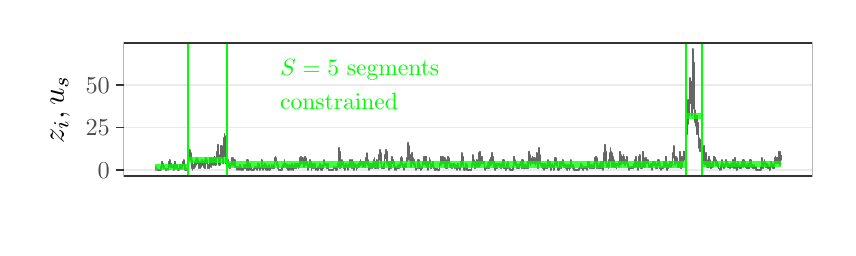
\begin{tikzpicture}[x=1pt,y=1pt]
\definecolor{fillColor}{RGB}{255,255,255}
\path[use as bounding box,fill=fillColor,fill opacity=0.00] (0,0) rectangle (289.08, 72.27);
\begin{scope}
\path[clip] (  0.00,  0.00) rectangle (289.08, 72.27);
\definecolor{drawColor}{RGB}{255,255,255}
\definecolor{fillColor}{RGB}{255,255,255}

\path[draw=drawColor,line width= 0.6pt,line join=round,line cap=round,fill=fillColor] (  0.00,  0.00) rectangle (289.08, 72.27);
\end{scope}
\begin{scope}
\path[clip] ( 34.65, 18.58) rectangle (283.58, 66.77);
\definecolor{fillColor}{RGB}{255,255,255}

\path[fill=fillColor] ( 34.65, 18.58) rectangle (283.58, 66.77);
\definecolor{drawColor}{gray}{0.92}

\path[draw=drawColor,line width= 0.6pt,line join=round] ( 34.65, 20.77) --
	(283.58, 20.77);

\path[draw=drawColor,line width= 0.6pt,line join=round] ( 34.65, 36.19) --
	(283.58, 36.19);

\path[draw=drawColor,line width= 0.6pt,line join=round] ( 34.65, 51.62) --
	(283.58, 51.62);
\definecolor{drawColor}{gray}{0.40}

\path[draw=drawColor,line width= 0.6pt,line join=round] ( 45.97, 21.38) --
	( 46.15, 21.38) --
	( 46.15, 20.77) --
	( 46.17, 20.77) --
	( 46.17, 21.38) --
	( 46.18, 21.38) --
	( 46.18, 22.00) --
	( 46.60, 22.00) --
	( 46.60, 21.38) --
	( 46.63, 21.38) --
	( 46.63, 20.77) --
	( 48.22, 20.77) --
	( 48.22, 21.38) --
	( 48.26, 21.38) --
	( 48.26, 22.00) --
	( 48.49, 22.00) --
	( 48.49, 22.62) --
	( 48.56, 22.62) --
	( 48.56, 23.23) --
	( 48.63, 23.23) --
	( 48.63, 23.85) --
	( 48.67, 23.85) --
	( 48.67, 23.23) --
	( 48.71, 23.23) --
	( 48.71, 22.62) --
	( 48.83, 22.62) --
	( 48.83, 23.23) --
	( 48.94, 23.23) --
	( 48.94, 22.62) --
	( 49.00, 22.62) --
	( 49.00, 23.23) --
	( 49.01, 23.23) --
	( 49.01, 22.62) --
	( 49.08, 22.62) --
	( 49.08, 22.00) --
	( 49.29, 22.00) --
	( 49.29, 21.38) --
	( 49.31, 21.38) --
	( 49.31, 22.00) --
	( 49.45, 22.00) --
	( 49.45, 21.38) --
	( 49.76, 21.38) --
	( 49.76, 20.77) --
	( 50.20, 20.77) --
	( 50.20, 21.38) --
	( 50.65, 21.38) --
	( 50.65, 20.77) --
	( 50.68, 20.77) --
	( 50.68, 21.38) --
	( 50.86, 21.38) --
	( 50.86, 22.00) --
	( 50.96, 22.00) --
	( 50.96, 22.62) --
	( 51.04, 22.62) --
	( 51.04, 23.23) --
	( 51.06, 23.23) --
	( 51.06, 23.85) --
	( 51.14, 23.85) --
	( 51.14, 23.23) --
	( 51.20, 23.23) --
	( 51.20, 23.85) --
	( 51.30, 23.85) --
	( 51.30, 24.47) --
	( 51.31, 24.47) --
	( 51.31, 23.85) --
	( 51.32, 23.85) --
	( 51.32, 24.47) --
	( 51.41, 24.47) --
	( 51.41, 23.85) --
	( 51.47, 23.85) --
	( 51.47, 24.47) --
	( 51.50, 24.47) --
	( 51.50, 23.85) --
	( 51.51, 23.85) --
	( 51.51, 23.23) --
	( 51.53, 23.23) --
	( 51.53, 23.85) --
	( 51.65, 23.85) --
	( 51.65, 23.23) --
	( 51.75, 23.23) --
	( 51.75, 22.62) --
	( 51.77, 22.62) --
	( 51.77, 22.00) --
	( 51.80, 22.00) --
	( 51.80, 22.62) --
	( 51.82, 22.62) --
	( 51.82, 23.23) --
	( 51.93, 23.23) --
	( 51.93, 22.62) --
	( 51.97, 22.62) --
	( 51.97, 22.00) --
	( 52.26, 22.00) --
	( 52.26, 22.62) --
	( 52.27, 22.62) --
	( 52.27, 22.00) --
	( 52.70, 22.00) --
	( 52.70, 20.77) --
	( 52.81, 20.77) --
	( 52.81, 21.38) --
	( 52.83, 21.38) --
	( 52.83, 22.00) --
	( 52.88, 22.00) --
	( 52.88, 22.62) --
	( 53.02, 22.62) --
	( 53.02, 23.23) --
	( 53.10, 23.23) --
	( 53.10, 23.85) --
	( 53.26, 23.85) --
	( 53.26, 23.23) --
	( 53.29, 23.23) --
	( 53.29, 22.62) --
	( 53.34, 22.62) --
	( 53.34, 22.00) --
	( 53.34, 22.00) --
	( 53.34, 22.62) --
	( 53.47, 22.62) --
	( 53.47, 22.00) --
	( 53.55, 22.00) --
	( 53.55, 21.38) --
	( 53.60, 21.38) --
	( 53.60, 22.00) --
	( 53.69, 22.00) --
	( 53.69, 22.62) --
	( 53.79, 22.62) --
	( 53.79, 22.00) --
	( 53.98, 22.00) --
	( 53.98, 22.62) --
	( 54.05, 22.62) --
	( 54.05, 22.00) --
	( 54.14, 22.00) --
	( 54.14, 21.38) --
	( 54.43, 21.38) --
	( 54.43, 20.77) --
	( 54.79, 20.77) --
	( 54.79, 21.38) --
	( 55.03, 21.38) --
	( 55.03, 22.00) --
	( 55.09, 22.00) --
	( 55.09, 22.62) --
	( 55.25, 22.62) --
	( 55.25, 22.00) --
	( 55.35, 22.00) --
	( 55.35, 22.62) --
	( 55.48, 22.62) --
	( 55.48, 22.00) --
	( 55.54, 22.00) --
	( 55.54, 21.38) --
	( 55.78, 21.38) --
	( 55.78, 22.00) --
	( 55.80, 22.00) --
	( 55.80, 21.38) --
	( 55.81, 21.38) --
	( 55.81, 22.00) --
	( 55.98, 22.00) --
	( 55.98, 23.23) --
	( 56.17, 23.23) --
	( 56.17, 23.85) --
	( 56.23, 23.85) --
	( 56.23, 23.23) --
	( 56.27, 23.23) --
	( 56.27, 22.62) --
	( 56.41, 22.62) --
	( 56.41, 23.85) --
	( 56.43, 23.85) --
	( 56.43, 24.47) --
	( 56.44, 24.47) --
	( 56.44, 23.23) --
	( 56.62, 23.23) --
	( 56.62, 22.62) --
	( 56.87, 22.62) --
	( 56.87, 21.38) --
	( 56.87, 21.38) --
	( 56.87, 20.77) --
	( 57.13, 20.77) --
	( 57.13, 21.38) --
	( 57.59, 21.38) --
	( 57.59, 20.77) --
	( 57.72, 20.77) --
	( 57.72, 21.38) --
	( 57.77, 21.38) --
	( 57.77, 22.00) --
	( 57.82, 22.00) --
	( 57.82, 23.23) --
	( 57.91, 23.23) --
	( 57.91, 24.47) --
	( 58.05, 24.47) --
	( 58.05, 25.09) --
	( 58.10, 25.09) --
	( 58.10, 25.70) --
	( 58.17, 25.70) --
	( 58.17, 25.09) --
	( 58.20, 25.09) --
	( 58.20, 26.94) --
	( 58.22, 26.94) --
	( 58.22, 27.55) --
	( 58.22, 27.55) --
	( 58.22, 26.94) --
	( 58.27, 26.94) --
	( 58.27, 28.17) --
	( 58.27, 28.17) --
	( 58.27, 26.94) --
	( 58.34, 26.94) --
	( 58.34, 27.55) --
	( 58.37, 27.55) --
	( 58.37, 26.32) --
	( 58.43, 26.32) --
	( 58.43, 26.94) --
	( 58.51, 26.94) --
	( 58.51, 26.32) --
	( 58.56, 26.32) --
	( 58.56, 25.70) --
	( 58.59, 25.70) --
	( 58.59, 27.55) --
	( 58.64, 27.55) --
	( 58.64, 28.17) --
	( 58.65, 28.17) --
	( 58.65, 27.55) --
	( 58.65, 27.55) --
	( 58.65, 26.32) --
	( 58.67, 26.32) --
	( 58.67, 25.70) --
	( 58.73, 25.70) --
	( 58.73, 24.47) --
	( 58.81, 24.47) --
	( 58.81, 25.09) --
	( 58.84, 25.09) --
	( 58.84, 25.70) --
	( 58.84, 25.70) --
	( 58.84, 26.32) --
	( 58.89, 26.32) --
	( 58.89, 25.70) --
	( 58.99, 25.70) --
	( 58.99, 26.32) --
	( 59.02, 26.32) --
	( 59.02, 26.94) --
	( 59.04, 26.94) --
	( 59.04, 25.09) --
	( 59.05, 25.09) --
	( 59.05, 25.70) --
	( 59.09, 25.70) --
	( 59.09, 25.09) --
	( 59.25, 25.09) --
	( 59.25, 24.47) --
	( 59.27, 24.47) --
	( 59.27, 23.85) --
	( 59.29, 23.85) --
	( 59.29, 22.62) --
	( 59.45, 22.62) --
	( 59.45, 21.38) --
	( 59.51, 21.38) --
	( 59.51, 20.77) --
	( 59.56, 20.77) --
	( 59.56, 21.38) --
	( 59.65, 21.38) --
	( 59.65, 22.00) --
	( 59.87, 22.00) --
	( 59.87, 22.62) --
	( 60.00, 22.62) --
	( 60.00, 22.00) --
	( 60.10, 22.00) --
	( 60.10, 21.38) --
	( 60.22, 21.38) --
	( 60.22, 22.00) --
	( 60.32, 22.00) --
	( 60.32, 21.38) --
	( 60.33, 21.38) --
	( 60.33, 22.00) --
	( 60.37, 22.00) --
	( 60.37, 22.62) --
	( 60.39, 22.62) --
	( 60.39, 23.23) --
	( 60.56, 23.23) --
	( 60.56, 23.85) --
	( 60.67, 23.85) --
	( 60.67, 23.23) --
	( 60.69, 23.23) --
	( 60.69, 23.85) --
	( 60.78, 23.85) --
	( 60.78, 23.23) --
	( 60.82, 23.23) --
	( 60.82, 22.62) --
	( 60.83, 22.62) --
	( 60.83, 23.85) --
	( 60.85, 23.85) --
	( 60.85, 23.23) --
	( 60.92, 23.23) --
	( 60.92, 23.85) --
	( 60.94, 23.85) --
	( 60.94, 24.47) --
	( 61.09, 24.47) --
	( 61.09, 25.09) --
	( 61.14, 25.09) --
	( 61.14, 24.47) --
	( 61.23, 24.47) --
	( 61.23, 25.09) --
	( 61.28, 25.09) --
	( 61.28, 23.85) --
	( 61.37, 23.85) --
	( 61.37, 24.47) --
	( 61.38, 24.47) --
	( 61.38, 23.85) --
	( 61.39, 23.85) --
	( 61.39, 23.23) --
	( 61.42, 23.23) --
	( 61.42, 24.47) --
	( 61.46, 24.47) --
	( 61.46, 23.85) --
	( 61.54, 23.85) --
	( 61.54, 23.23) --
	( 61.68, 23.23) --
	( 61.68, 22.62) --
	( 61.79, 22.62) --
	( 61.79, 23.23) --
	( 61.82, 23.23) --
	( 61.82, 22.62) --
	( 61.88, 22.62) --
	( 61.88, 21.38) --
	( 61.89, 21.38) --
	( 61.89, 22.00) --
	( 61.91, 22.00) --
	( 61.91, 22.62) --
	( 61.96, 22.62) --
	( 61.96, 23.23) --
	( 62.22, 23.23) --
	( 62.22, 23.85) --
	( 62.23, 23.85) --
	( 62.23, 23.23) --
	( 62.34, 23.23) --
	( 62.34, 22.62) --
	( 62.36, 22.62) --
	( 62.36, 22.00) --
	( 62.42, 22.00) --
	( 62.42, 21.38) --
	( 62.50, 21.38) --
	( 62.50, 22.00) --
	( 62.61, 22.00) --
	( 62.61, 22.62) --
	( 62.63, 22.62) --
	( 62.63, 23.23) --
	( 62.64, 23.23) --
	( 62.64, 23.85) --
	( 62.66, 23.85) --
	( 62.66, 23.23) --
	( 62.68, 23.23) --
	( 62.68, 23.85) --
	( 62.75, 23.85) --
	( 62.75, 24.47) --
	( 62.95, 24.47) --
	( 62.95, 23.85) --
	( 63.03, 23.85) --
	( 63.03, 24.47) --
	( 63.09, 24.47) --
	( 63.09, 23.85) --
	( 63.09, 23.85) --
	( 63.09, 23.23) --
	( 63.10, 23.23) --
	( 63.10, 23.85) --
	( 63.14, 23.85) --
	( 63.14, 23.23) --
	( 63.20, 23.23) --
	( 63.20, 22.62) --
	( 63.42, 22.62) --
	( 63.42, 23.23) --
	( 63.45, 23.23) --
	( 63.45, 23.85) --
	( 63.48, 23.85) --
	( 63.48, 23.23) --
	( 63.51, 23.23) --
	( 63.51, 22.62) --
	( 63.55, 22.62) --
	( 63.55, 22.00) --
	( 63.86, 22.00) --
	( 63.86, 22.62) --
	( 63.87, 22.62) --
	( 63.87, 22.00) --
	( 63.91, 22.00) --
	( 63.91, 21.38) --
	( 63.96, 21.38) --
	( 63.96, 22.00) --
	( 63.97, 22.00) --
	( 63.97, 22.62) --
	( 64.06, 22.62) --
	( 64.06, 23.23) --
	( 64.14, 23.23) --
	( 64.14, 23.85) --
	( 64.17, 23.85) --
	( 64.17, 24.47) --
	( 64.25, 24.47) --
	( 64.25, 25.09) --
	( 64.31, 25.09) --
	( 64.31, 24.47) --
	( 64.39, 24.47) --
	( 64.39, 25.09) --
	( 64.41, 25.09) --
	( 64.41, 24.47) --
	( 64.42, 24.47) --
	( 64.42, 23.85) --
	( 64.48, 23.85) --
	( 64.48, 23.23) --
	( 64.52, 23.23) --
	( 64.52, 23.85) --
	( 64.58, 23.85) --
	( 64.58, 24.47) --
	( 64.59, 24.47) --
	( 64.59, 23.85) --
	( 64.60, 23.85) --
	( 64.60, 24.47) --
	( 64.62, 24.47) --
	( 64.62, 23.85) --
	( 64.65, 23.85) --
	( 64.65, 24.47) --
	( 64.71, 24.47) --
	( 64.71, 23.85) --
	( 64.76, 23.85) --
	( 64.76, 24.47) --
	( 64.85, 24.47) --
	( 64.85, 23.85) --
	( 64.97, 23.85) --
	( 64.97, 23.23) --
	( 65.04, 23.23) --
	( 65.04, 22.62) --
	( 65.05, 22.62) --
	( 65.05, 22.00) --
	( 65.10, 22.00) --
	( 65.10, 21.38) --
	( 65.13, 21.38) --
	( 65.13, 22.00) --
	( 65.15, 22.00) --
	( 65.15, 21.38) --
	( 65.28, 21.38) --
	( 65.28, 22.00) --
	( 65.53, 22.00) --
	( 65.53, 22.62) --
	( 65.58, 22.62) --
	( 65.58, 22.00) --
	( 65.73, 22.00) --
	( 65.73, 21.38) --
	( 65.76, 21.38) --
	( 65.76, 22.62) --
	( 65.78, 22.62) --
	( 65.78, 23.23) --
	( 65.80, 23.23) --
	( 65.80, 23.85) --
	( 65.82, 23.85) --
	( 65.82, 24.47) --
	( 65.86, 24.47) --
	( 65.86, 25.09) --
	( 65.98, 25.09) --
	( 65.98, 24.47) --
	( 66.05, 24.47) --
	( 66.05, 25.09) --
	( 66.21, 25.09) --
	( 66.21, 23.85) --
	( 66.24, 23.85) --
	( 66.24, 23.23) --
	( 66.24, 23.23) --
	( 66.24, 22.62) --
	( 66.31, 22.62) --
	( 66.31, 22.00) --
	( 66.39, 22.00) --
	( 66.39, 22.62) --
	( 66.41, 22.62) --
	( 66.41, 23.85) --
	( 66.53, 23.85) --
	( 66.53, 24.47) --
	( 66.58, 24.47) --
	( 66.58, 25.09) --
	( 66.72, 25.09) --
	( 66.72, 24.47) --
	( 66.84, 24.47) --
	( 66.84, 23.85) --
	( 66.86, 23.85) --
	( 66.86, 22.62) --
	( 66.89, 22.62) --
	( 66.89, 23.23) --
	( 66.96, 23.23) --
	( 66.96, 22.62) --
	( 66.98, 22.62) --
	( 66.98, 23.23) --
	( 66.99, 23.23) --
	( 66.99, 22.62) --
	( 67.02, 22.62) --
	( 67.02, 23.23) --
	( 67.03, 23.23) --
	( 67.03, 22.62) --
	( 67.09, 22.62) --
	( 67.09, 23.23) --
	( 67.16, 23.23) --
	( 67.16, 23.85) --
	( 67.19, 23.85) --
	( 67.19, 24.47) --
	( 67.27, 24.47) --
	( 67.27, 25.09) --
	( 67.34, 25.09) --
	( 67.34, 24.47) --
	( 67.34, 24.47) --
	( 67.34, 25.09) --
	( 67.43, 25.09) --
	( 67.43, 24.47) --
	( 67.46, 24.47) --
	( 67.46, 25.09) --
	( 67.47, 25.09) --
	( 67.47, 25.70) --
	( 67.48, 25.70) --
	( 67.48, 25.09) --
	( 67.54, 25.09) --
	( 67.54, 24.47) --
	( 67.62, 24.47) --
	( 67.62, 23.85) --
	( 67.64, 23.85) --
	( 67.64, 23.23) --
	( 67.72, 23.23) --
	( 67.72, 22.62) --
	( 67.73, 22.62) --
	( 67.73, 23.23) --
	( 67.76, 23.23) --
	( 67.76, 24.47) --
	( 67.80, 24.47) --
	( 67.80, 23.85) --
	( 67.91, 23.85) --
	( 67.91, 23.23) --
	( 67.92, 23.23) --
	( 67.92, 22.62) --
	( 67.94, 22.62) --
	( 67.94, 23.23) --
	( 67.99, 23.23) --
	( 67.99, 23.85) --
	( 68.06, 23.85) --
	( 68.06, 24.47) --
	( 68.16, 24.47) --
	( 68.16, 25.09) --
	( 68.18, 25.09) --
	( 68.18, 24.47) --
	( 68.20, 24.47) --
	( 68.20, 25.09) --
	( 68.20, 25.09) --
	( 68.20, 25.70) --
	( 68.21, 25.70) --
	( 68.21, 25.09) --
	( 68.21, 25.09) --
	( 68.21, 24.47) --
	( 68.24, 24.47) --
	( 68.24, 25.09) --
	( 68.39, 25.09) --
	( 68.39, 25.70) --
	( 68.39, 25.70) --
	( 68.39, 25.09) --
	( 68.44, 25.09) --
	( 68.44, 25.70) --
	( 68.44, 25.70) --
	( 68.44, 25.09) --
	( 68.46, 25.09) --
	( 68.46, 26.94) --
	( 68.47, 26.94) --
	( 68.47, 27.55) --
	( 68.49, 27.55) --
	( 68.49, 26.94) --
	( 68.51, 26.94) --
	( 68.51, 27.55) --
	( 68.56, 27.55) --
	( 68.56, 28.17) --
	( 68.60, 28.17) --
	( 68.60, 28.79) --
	( 68.61, 28.79) --
	( 68.61, 28.17) --
	( 68.65, 28.17) --
	( 68.65, 27.55) --
	( 68.66, 27.55) --
	( 68.66, 26.94) --
	( 68.66, 26.94) --
	( 68.66, 27.55) --
	( 68.69, 27.55) --
	( 68.69, 28.17) --
	( 68.69, 28.17) --
	( 68.69, 27.55) --
	( 68.70, 27.55) --
	( 68.70, 28.79) --
	( 68.77, 28.79) --
	( 68.77, 29.41) --
	( 68.83, 29.41) --
	( 68.83, 30.02) --
	( 68.83, 30.02) --
	( 68.83, 29.41) --
	( 68.89, 29.41) --
	( 68.89, 28.79) --
	( 68.92, 28.79) --
	( 68.92, 26.94) --
	( 68.92, 26.94) --
	( 68.92, 25.70) --
	( 68.93, 25.70) --
	( 68.93, 26.32) --
	( 68.99, 26.32) --
	( 68.99, 26.94) --
	( 69.01, 26.94) --
	( 69.01, 26.32) --
	( 69.05, 26.32) --
	( 69.05, 25.70) --
	( 69.06, 25.70) --
	( 69.06, 25.09) --
	( 69.14, 25.09) --
	( 69.14, 24.47) --
	( 69.16, 24.47) --
	( 69.16, 23.23) --
	( 69.20, 23.23) --
	( 69.20, 23.85) --
	( 69.21, 23.85) --
	( 69.21, 22.62) --
	( 69.30, 22.62) --
	( 69.30, 23.23) --
	( 69.38, 23.23) --
	( 69.38, 23.85) --
	( 69.39, 23.85) --
	( 69.39, 23.23) --
	( 69.44, 23.23) --
	( 69.44, 22.62) --
	( 69.51, 22.62) --
	( 69.51, 23.85) --
	( 69.55, 23.85) --
	( 69.55, 24.47) --
	( 69.59, 24.47) --
	( 69.59, 25.09) --
	( 69.59, 25.09) --
	( 69.59, 24.47) --
	( 69.66, 24.47) --
	( 69.66, 25.09) --
	( 69.68, 25.09) --
	( 69.68, 25.70) --
	( 69.75, 25.70) --
	( 69.75, 25.09) --
	( 69.78, 25.09) --
	( 69.78, 25.70) --
	( 69.79, 25.70) --
	( 69.79, 26.32) --
	( 69.82, 26.32) --
	( 69.82, 26.94) --
	( 69.85, 26.94) --
	( 69.85, 26.32) --
	( 69.87, 26.32) --
	( 69.87, 26.94) --
	( 69.90, 26.94) --
	( 69.90, 27.55) --
	( 69.92, 27.55) --
	( 69.92, 28.17) --
	( 69.92, 28.17) --
	( 69.92, 28.79) --
	( 69.97, 28.79) --
	( 69.97, 29.41) --
	( 70.00, 29.41) --
	( 70.00, 28.79) --
	( 70.02, 28.79) --
	( 70.02, 29.41) --
	( 70.04, 29.41) --
	( 70.04, 28.79) --
	( 70.05, 28.79) --
	( 70.05, 28.17) --
	( 70.08, 28.17) --
	( 70.08, 28.79) --
	( 70.09, 28.79) --
	( 70.09, 29.41) --
	( 70.11, 29.41) --
	( 70.11, 28.79) --
	( 70.19, 28.79) --
	( 70.19, 29.41) --
	( 70.24, 29.41) --
	( 70.24, 28.79) --
	( 70.27, 28.79) --
	( 70.27, 28.17) --
	( 70.28, 28.17) --
	( 70.28, 28.79) --
	( 70.29, 28.79) --
	( 70.29, 28.17) --
	( 70.32, 28.17) --
	( 70.32, 28.79) --
	( 70.35, 28.79) --
	( 70.35, 28.17) --
	( 70.37, 28.17) --
	( 70.37, 27.55) --
	( 70.38, 27.55) --
	( 70.38, 26.94) --
	( 70.41, 26.94) --
	( 70.41, 26.32) --
	( 70.43, 26.32) --
	( 70.43, 25.70) --
	( 70.47, 25.70) --
	( 70.47, 25.09) --
	( 70.52, 25.09) --
	( 70.52, 24.47) --
	( 70.53, 24.47) --
	( 70.53, 25.09) --
	( 70.54, 25.09) --
	( 70.54, 24.47) --
	( 70.54, 24.47) --
	( 70.54, 23.85) --
	( 70.59, 23.85) --
	( 70.59, 23.23) --
	( 70.60, 23.23) --
	( 70.60, 23.85) --
	( 70.63, 23.85) --
	( 70.63, 24.47) --
	( 70.64, 24.47) --
	( 70.64, 23.85) --
	( 70.72, 23.85) --
	( 70.72, 24.47) --
	( 70.73, 24.47) --
	( 70.73, 23.85) --
	( 70.77, 23.85) --
	( 70.77, 23.23) --
	( 70.79, 23.23) --
	( 70.79, 23.85) --
	( 70.79, 23.85) --
	( 70.79, 25.09) --
	( 70.80, 25.09) --
	( 70.80, 25.70) --
	( 70.86, 25.70) --
	( 70.86, 26.32) --
	( 70.89, 26.32) --
	( 70.89, 26.94) --
	( 70.91, 26.94) --
	( 70.91, 27.55) --
	( 70.91, 27.55) --
	( 70.91, 28.17) --
	( 70.95, 28.17) --
	( 70.95, 28.79) --
	( 70.97, 28.79) --
	( 70.97, 29.41) --
	( 70.98, 29.41) --
	( 70.98, 28.79) --
	( 70.98, 28.79) --
	( 70.98, 29.41) --
	( 71.00, 29.41) --
	( 71.00, 31.26) --
	( 71.02, 31.26) --
	( 71.02, 31.87) --
	( 71.04, 31.87) --
	( 71.04, 31.26) --
	( 71.05, 31.26) --
	( 71.05, 31.87) --
	( 71.06, 31.87) --
	( 71.06, 32.49) --
	( 71.07, 32.49) --
	( 71.07, 33.11) --
	( 71.08, 33.11) --
	( 71.08, 33.73) --
	( 71.09, 33.73) --
	( 71.09, 33.11) --
	( 71.14, 33.11) --
	( 71.14, 33.73) --
	( 71.17, 33.73) --
	( 71.17, 33.11) --
	( 71.24, 33.11) --
	( 71.24, 32.49) --
	( 71.25, 32.49) --
	( 71.25, 31.87) --
	( 71.26, 31.87) --
	( 71.26, 31.26) --
	( 71.31, 31.26) --
	( 71.31, 30.64) --
	( 71.35, 30.64) --
	( 71.35, 30.02) --
	( 71.36, 30.02) --
	( 71.36, 29.41) --
	( 71.36, 29.41) --
	( 71.36, 28.79) --
	( 71.40, 28.79) --
	( 71.40, 28.17) --
	( 71.42, 28.17) --
	( 71.42, 27.55) --
	( 71.44, 27.55) --
	( 71.44, 26.94) --
	( 71.45, 26.94) --
	( 71.45, 25.09) --
	( 71.46, 25.09) --
	( 71.46, 25.70) --
	( 71.47, 25.70) --
	( 71.47, 24.47) --
	( 71.50, 24.47) --
	( 71.50, 23.85) --
	( 71.51, 23.85) --
	( 71.51, 23.23) --
	( 71.52, 23.23) --
	( 71.52, 23.85) --
	( 71.53, 23.85) --
	( 71.53, 24.47) --
	( 71.54, 24.47) --
	( 71.54, 23.85) --
	( 71.59, 23.85) --
	( 71.59, 23.23) --
	( 71.71, 23.23) --
	( 71.71, 24.47) --
	( 71.91, 24.47) --
	( 71.91, 23.85) --
	( 71.97, 23.85) --
	( 71.97, 22.00) --
	( 72.14, 22.00) --
	( 72.14, 23.23) --
	( 72.16, 23.23) --
	( 72.16, 22.00) --
	( 72.25, 22.00) --
	( 72.25, 22.62) --
	( 72.38, 22.62) --
	( 72.38, 23.23) --
	( 72.52, 23.23) --
	( 72.52, 23.85) --
	( 72.53, 23.85) --
	( 72.53, 24.47) --
	( 72.59, 24.47) --
	( 72.59, 23.23) --
	( 72.69, 23.23) --
	( 72.69, 22.62) --
	( 72.83, 22.62) --
	( 72.83, 22.00) --
	( 72.84, 22.00) --
	( 72.84, 22.62) --
	( 72.97, 22.62) --
	( 72.97, 22.00) --
	( 72.98, 22.00) --
	( 72.98, 21.38) --
	( 73.00, 21.38) --
	( 73.00, 22.00) --
	( 73.01, 22.00) --
	( 73.01, 22.62) --
	( 73.28, 22.62) --
	( 73.28, 23.23) --
	( 73.29, 23.23) --
	( 73.29, 22.62) --
	( 73.43, 22.62) --
	( 73.43, 23.23) --
	( 73.46, 23.23) --
	( 73.46, 22.62) --
	( 73.53, 22.62) --
	( 73.53, 23.23) --
	( 73.66, 23.23) --
	( 73.66, 23.85) --
	( 73.73, 23.85) --
	( 73.73, 23.23) --
	( 73.77, 23.23) --
	( 73.77, 23.85) --
	( 73.83, 23.85) --
	( 73.83, 25.09) --
	( 73.88, 25.09) --
	( 73.88, 24.47) --
	( 73.91, 24.47) --
	( 73.91, 23.85) --
	( 73.98, 23.85) --
	( 73.98, 23.23) --
	( 74.03, 23.23) --
	( 74.03, 23.85) --
	( 74.05, 23.85) --
	( 74.05, 24.47) --
	( 74.11, 24.47) --
	( 74.11, 23.85) --
	( 74.16, 23.85) --
	( 74.16, 24.47) --
	( 74.20, 24.47) --
	( 74.20, 25.09) --
	( 74.21, 25.09) --
	( 74.21, 24.47) --
	( 74.21, 24.47) --
	( 74.21, 23.85) --
	( 74.24, 23.85) --
	( 74.24, 23.23) --
	( 74.28, 23.23) --
	( 74.28, 22.62) --
	( 74.36, 22.62) --
	( 74.36, 23.23) --
	( 74.38, 23.23) --
	( 74.38, 23.85) --
	( 74.41, 23.85) --
	( 74.41, 23.23) --
	( 74.50, 23.23) --
	( 74.50, 22.62) --
	( 74.52, 22.62) --
	( 74.52, 23.23) --
	( 74.52, 23.23) --
	( 74.52, 23.85) --
	( 74.62, 23.85) --
	( 74.62, 24.47) --
	( 74.65, 24.47) --
	( 74.65, 23.85) --
	( 74.65, 23.85) --
	( 74.65, 24.47) --
	( 74.81, 24.47) --
	( 74.81, 23.85) --
	( 74.83, 23.85) --
	( 74.83, 23.23) --
	( 74.97, 23.23) --
	( 74.97, 22.00) --
	( 75.05, 22.00) --
	( 75.05, 22.62) --
	( 75.07, 22.62) --
	( 75.07, 22.00) --
	( 75.08, 22.00) --
	( 75.08, 22.62) --
	( 75.10, 22.62) --
	( 75.10, 22.00) --
	( 75.50, 22.00) --
	( 75.50, 21.38) --
	( 75.53, 21.38) --
	( 75.53, 20.77) --
	( 75.72, 20.77) --
	( 75.72, 21.38) --
	( 75.83, 21.38) --
	( 75.83, 22.00) --
	( 76.12, 22.00) --
	( 76.12, 21.38) --
	( 76.28, 21.38) --
	( 76.28, 20.77) --
	( 76.47, 20.77) --
	( 76.47, 21.38) --
	( 76.53, 21.38) --
	( 76.53, 22.00) --
	( 76.54, 22.00) --
	( 76.54, 22.62) --
	( 76.92, 22.62) --
	( 76.92, 22.00) --
	( 76.98, 22.00) --
	( 76.98, 21.38) --
	( 76.99, 21.38) --
	( 76.99, 20.77) --
	( 77.22, 20.77) --
	( 77.22, 21.38) --
	( 77.68, 21.38) --
	( 77.68, 20.77) --
	( 77.89, 20.77) --
	( 77.89, 21.38) --
	( 78.03, 21.38) --
	( 78.03, 22.00) --
	( 78.20, 22.00) --
	( 78.20, 22.62) --
	( 78.24, 22.62) --
	( 78.24, 22.00) --
	( 78.35, 22.00) --
	( 78.35, 21.38) --
	( 78.51, 21.38) --
	( 78.51, 22.00) --
	( 78.57, 22.00) --
	( 78.57, 22.62) --
	( 78.65, 22.62) --
	( 78.65, 22.00) --
	( 78.96, 22.00) --
	( 78.96, 21.38) --
	( 79.02, 21.38) --
	( 79.02, 20.77) --
	( 79.20, 20.77) --
	( 79.20, 22.62) --
	( 79.23, 22.62) --
	( 79.23, 24.47) --
	( 79.65, 24.47) --
	( 79.65, 22.62) --
	( 79.68, 22.62) --
	( 79.68, 22.00) --
	( 79.68, 22.00) --
	( 79.68, 20.77) --
	( 79.93, 20.77) --
	( 79.93, 21.38) --
	( 79.96, 21.38) --
	( 79.96, 22.00) --
	( 80.14, 22.00) --
	( 80.14, 22.62) --
	( 80.29, 22.62) --
	( 80.29, 23.23) --
	( 80.35, 23.23) --
	( 80.35, 22.62) --
	( 80.41, 22.62) --
	( 80.41, 22.00) --
	( 80.59, 22.00) --
	( 80.59, 21.38) --
	( 80.74, 21.38) --
	( 80.74, 20.77) --
	( 81.79, 20.77) --
	( 81.79, 21.38) --
	( 82.03, 21.38) --
	( 82.03, 22.00) --
	( 82.24, 22.00) --
	( 82.24, 21.38) --
	( 82.27, 21.38) --
	( 82.27, 22.00) --
	( 82.48, 22.00) --
	( 82.48, 21.38) --
	( 82.53, 21.38) --
	( 82.53, 22.00) --
	( 82.72, 22.00) --
	( 82.72, 21.38) --
	( 82.98, 21.38) --
	( 82.98, 20.77) --
	( 83.02, 20.77) --
	( 83.02, 21.38) --
	( 83.25, 21.38) --
	( 83.25, 22.00) --
	( 83.28, 22.00) --
	( 83.28, 22.62) --
	( 83.29, 22.62) --
	( 83.29, 23.23) --
	( 83.47, 23.23) --
	( 83.47, 22.62) --
	( 83.71, 22.62) --
	( 83.71, 22.00) --
	( 83.73, 22.00) --
	( 83.73, 21.38) --
	( 83.74, 21.38) --
	( 83.74, 20.77) --
	( 83.85, 20.77) --
	( 83.85, 21.38) --
	( 84.23, 21.38) --
	( 84.23, 22.00) --
	( 84.30, 22.00) --
	( 84.30, 21.38) --
	( 84.38, 21.38) --
	( 84.38, 22.00) --
	( 84.46, 22.00) --
	( 84.46, 22.62) --
	( 84.49, 22.62) --
	( 84.49, 23.85) --
	( 84.51, 23.85) --
	( 84.51, 24.47) --
	( 84.68, 24.47) --
	( 84.68, 23.85) --
	( 84.83, 23.85) --
	( 84.83, 23.23) --
	( 84.91, 23.23) --
	( 84.91, 22.62) --
	( 84.95, 22.62) --
	( 84.95, 21.38) --
	( 84.96, 21.38) --
	( 84.96, 20.77) --
	( 84.99, 20.77) --
	( 84.99, 21.38) --
	( 85.22, 21.38) --
	( 85.22, 22.00) --
	( 85.44, 22.00) --
	( 85.44, 21.38) --
	( 85.57, 21.38) --
	( 85.57, 22.00) --
	( 85.63, 22.00) --
	( 85.63, 23.23) --
	( 85.67, 23.23) --
	( 85.67, 22.62) --
	( 86.02, 22.62) --
	( 86.02, 22.00) --
	( 86.08, 22.00) --
	( 86.08, 20.77) --
	( 86.14, 20.77) --
	( 86.14, 21.38) --
	( 86.38, 21.38) --
	( 86.38, 22.00) --
	( 86.59, 22.00) --
	( 86.59, 20.77) --
	( 86.66, 20.77) --
	( 86.66, 21.38) --
	( 86.80, 21.38) --
	( 86.80, 22.00) --
	( 87.05, 22.00) --
	( 87.05, 22.62) --
	( 87.09, 22.62) --
	( 87.09, 22.00) --
	( 87.24, 22.00) --
	( 87.24, 20.77) --
	( 87.50, 20.77) --
	( 87.50, 21.38) --
	( 87.93, 21.38) --
	( 87.93, 22.00) --
	( 87.95, 22.00) --
	( 87.95, 21.38) --
	( 88.03, 21.38) --
	( 88.03, 22.00) --
	( 88.20, 22.00) --
	( 88.20, 22.62) --
	( 88.38, 22.62) --
	( 88.38, 22.00) --
	( 88.49, 22.00) --
	( 88.49, 21.38) --
	( 88.50, 21.38) --
	( 88.50, 22.00) --
	( 88.63, 22.00) --
	( 88.63, 21.38) --
	( 88.76, 21.38) --
	( 88.76, 22.00) --
	( 88.95, 22.00) --
	( 88.95, 21.38) --
	( 89.11, 21.38) --
	( 89.11, 22.00) --
	( 89.12, 22.00) --
	( 89.12, 22.62) --
	( 89.17, 22.62) --
	( 89.17, 23.85) --
	( 89.21, 23.85) --
	( 89.21, 23.23) --
	( 89.25, 23.23) --
	( 89.25, 23.85) --
	( 89.28, 23.85) --
	( 89.28, 24.47) --
	( 89.39, 24.47) --
	( 89.39, 25.09) --
	( 89.50, 25.09) --
	( 89.50, 25.70) --
	( 89.56, 25.70) --
	( 89.56, 25.09) --
	( 89.57, 25.09) --
	( 89.57, 25.70) --
	( 89.58, 25.70) --
	( 89.58, 25.09) --
	( 89.63, 25.09) --
	( 89.63, 23.85) --
	( 89.69, 23.85) --
	( 89.69, 24.47) --
	( 89.70, 24.47) --
	( 89.70, 23.85) --
	( 89.71, 23.85) --
	( 89.71, 24.47) --
	( 89.73, 24.47) --
	( 89.73, 23.85) --
	( 89.81, 23.85) --
	( 89.81, 24.47) --
	( 89.84, 24.47) --
	( 89.84, 23.85) --
	( 89.95, 23.85) --
	( 89.95, 23.23) --
	( 89.99, 23.23) --
	( 89.99, 23.85) --
	( 90.02, 23.85) --
	( 90.02, 23.23) --
	( 90.08, 23.23) --
	( 90.08, 23.85) --
	( 90.15, 23.85) --
	( 90.15, 23.23) --
	( 90.15, 23.23) --
	( 90.15, 22.62) --
	( 90.22, 22.62) --
	( 90.22, 23.23) --
	( 90.26, 23.23) --
	( 90.26, 22.62) --
	( 90.44, 22.62) --
	( 90.44, 22.00) --
	( 90.54, 22.00) --
	( 90.54, 21.38) --
	( 90.68, 21.38) --
	( 90.68, 20.77) --
	( 91.91, 20.77) --
	( 91.91, 21.38) --
	( 91.93, 21.38) --
	( 91.93, 22.00) --
	( 92.07, 22.00) --
	( 92.07, 22.62) --
	( 92.35, 22.62) --
	( 92.35, 22.00) --
	( 92.36, 22.00) --
	( 92.36, 22.62) --
	( 92.38, 22.62) --
	( 92.38, 23.23) --
	( 92.39, 23.23) --
	( 92.39, 22.62) --
	( 92.53, 22.62) --
	( 92.53, 22.00) --
	( 92.61, 22.00) --
	( 92.61, 22.62) --
	( 92.69, 22.62) --
	( 92.69, 23.23) --
	( 92.79, 23.23) --
	( 92.79, 24.47) --
	( 92.81, 24.47) --
	( 92.81, 23.85) --
	( 92.83, 23.85) --
	( 92.83, 23.23) --
	( 93.07, 23.23) --
	( 93.07, 22.62) --
	( 93.11, 22.62) --
	( 93.11, 23.23) --
	( 93.14, 23.23) --
	( 93.14, 22.62) --
	( 93.16, 22.62) --
	( 93.16, 23.23) --
	( 93.24, 23.23) --
	( 93.24, 22.00) --
	( 93.52, 22.00) --
	( 93.52, 22.62) --
	( 93.56, 22.62) --
	( 93.56, 22.00) --
	( 93.61, 22.00) --
	( 93.61, 21.38) --
	( 93.64, 21.38) --
	( 93.64, 22.00) --
	( 93.72, 22.00) --
	( 93.72, 22.62) --
	( 93.97, 22.62) --
	( 93.97, 22.00) --
	( 94.09, 22.00) --
	( 94.09, 21.38) --
	( 94.17, 21.38) --
	( 94.17, 20.77) --
	( 94.42, 20.77) --
	( 94.42, 21.38) --
	( 94.42, 21.38) --
	( 94.42, 22.00) --
	( 94.75, 22.00) --
	( 94.75, 22.62) --
	( 94.87, 22.62) --
	( 94.87, 21.38) --
	( 95.20, 21.38) --
	( 95.20, 20.77) --
	( 95.22, 20.77) --
	( 95.22, 21.38) --
	( 95.39, 21.38) --
	( 95.39, 22.00) --
	( 95.47, 22.00) --
	( 95.47, 22.62) --
	( 95.50, 22.62) --
	( 95.50, 23.23) --
	( 95.67, 23.23) --
	( 95.67, 22.62) --
	( 95.84, 22.62) --
	( 95.84, 22.00) --
	( 95.92, 22.00) --
	( 95.92, 21.38) --
	( 95.95, 21.38) --
	( 95.95, 20.77) --
	( 96.00, 20.77) --
	( 96.00, 21.38) --
	( 96.37, 21.38) --
	( 96.37, 22.00) --
	( 96.44, 22.00) --
	( 96.44, 22.62) --
	( 96.45, 22.62) --
	( 96.45, 22.00) --
	( 96.46, 22.00) --
	( 96.46, 22.62) --
	( 96.56, 22.62) --
	( 96.56, 23.23) --
	( 96.82, 23.23) --
	( 96.82, 22.62) --
	( 96.84, 22.62) --
	( 96.84, 23.23) --
	( 96.89, 23.23) --
	( 96.89, 22.62) --
	( 96.90, 22.62) --
	( 96.90, 22.00) --
	( 97.01, 22.00) --
	( 97.01, 21.38) --
	( 97.14, 21.38) --
	( 97.14, 22.00) --
	( 97.22, 22.00) --
	( 97.22, 22.62) --
	( 97.30, 22.62) --
	( 97.30, 22.00) --
	( 97.36, 22.00) --
	( 97.36, 22.62) --
	( 97.44, 22.62) --
	( 97.44, 23.23) --
	( 97.58, 23.23) --
	( 97.58, 22.62) --
	( 97.60, 22.62) --
	( 97.60, 23.23) --
	( 97.67, 23.23) --
	( 97.67, 22.62) --
	( 97.81, 22.62) --
	( 97.81, 22.00) --
	( 97.89, 22.00) --
	( 97.89, 21.38) --
	( 97.92, 21.38) --
	( 97.92, 22.00) --
	( 97.95, 22.00) --
	( 97.95, 22.62) --
	( 98.06, 22.62) --
	( 98.06, 22.00) --
	( 98.11, 22.00) --
	( 98.11, 22.62) --
	( 98.19, 22.62) --
	( 98.19, 22.00) --
	( 98.21, 22.00) --
	( 98.21, 22.62) --
	( 98.32, 22.62) --
	( 98.32, 23.23) --
	( 98.36, 23.23) --
	( 98.36, 23.85) --
	( 98.42, 23.85) --
	( 98.42, 24.47) --
	( 98.51, 24.47) --
	( 98.51, 25.09) --
	( 98.56, 25.09) --
	( 98.56, 24.47) --
	( 98.65, 24.47) --
	( 98.65, 23.85) --
	( 98.70, 23.85) --
	( 98.70, 24.47) --
	( 98.70, 24.47) --
	( 98.70, 25.09) --
	( 98.76, 25.09) --
	( 98.76, 25.70) --
	( 98.77, 25.70) --
	( 98.77, 25.09) --
	( 98.81, 25.09) --
	( 98.81, 24.47) --
	( 98.84, 24.47) --
	( 98.84, 25.09) --
	( 98.85, 25.09) --
	( 98.85, 23.85) --
	( 98.96, 23.85) --
	( 98.96, 23.23) --
	( 98.96, 23.23) --
	( 98.96, 23.85) --
	( 99.12, 23.85) --
	( 99.12, 24.47) --
	( 99.15, 24.47) --
	( 99.15, 23.85) --
	( 99.16, 23.85) --
	( 99.16, 23.23) --
	( 99.16, 23.23) --
	( 99.16, 23.85) --
	( 99.19, 23.85) --
	( 99.19, 24.47) --
	( 99.21, 24.47) --
	( 99.21, 25.09) --
	( 99.22, 25.09) --
	( 99.22, 24.47) --
	( 99.25, 24.47) --
	( 99.25, 25.09) --
	( 99.29, 25.09) --
	( 99.29, 24.47) --
	( 99.39, 24.47) --
	( 99.39, 25.09) --
	( 99.41, 25.09) --
	( 99.41, 24.47) --
	( 99.50, 24.47) --
	( 99.50, 25.09) --
	( 99.57, 25.09) --
	( 99.57, 24.47) --
	( 99.61, 24.47) --
	( 99.61, 23.85) --
	( 99.64, 23.85) --
	( 99.64, 23.23) --
	( 99.65, 23.23) --
	( 99.65, 23.85) --
	( 99.70, 23.85) --
	( 99.70, 23.23) --
	( 99.84, 23.23) --
	( 99.84, 22.62) --
	( 99.86, 22.62) --
	( 99.86, 22.00) --
	( 99.89, 22.00) --
	( 99.89, 22.62) --
	( 99.89, 22.62) --
	( 99.89, 23.23) --
	(100.10, 23.23) --
	(100.10, 22.62) --
	(100.18, 22.62) --
	(100.18, 23.23) --
	(100.24, 23.23) --
	(100.24, 23.85) --
	(100.26, 23.85) --
	(100.26, 24.47) --
	(100.32, 24.47) --
	(100.32, 25.70) --
	(100.34, 25.70) --
	(100.34, 25.09) --
	(100.34, 25.09) --
	(100.34, 24.47) --
	(100.38, 24.47) --
	(100.38, 25.09) --
	(100.40, 25.09) --
	(100.40, 24.47) --
	(100.49, 24.47) --
	(100.49, 25.09) --
	(100.63, 25.09) --
	(100.63, 24.47) --
	(100.68, 24.47) --
	(100.68, 23.85) --
	(100.71, 23.85) --
	(100.71, 23.23) --
	(100.74, 23.23) --
	(100.74, 24.47) --
	(100.77, 24.47) --
	(100.77, 23.85) --
	(100.77, 23.85) --
	(100.77, 23.23) --
	(100.78, 23.23) --
	(100.78, 23.85) --
	(100.83, 23.85) --
	(100.83, 23.23) --
	(100.94, 23.23) --
	(100.94, 22.62) --
	(101.19, 22.62) --
	(101.19, 21.38) --
	(101.23, 21.38) --
	(101.23, 20.77) --
	(101.29, 20.77) --
	(101.29, 21.38) --
	(101.52, 21.38) --
	(101.52, 22.00) --
	(101.68, 22.00) --
	(101.68, 22.62) --
	(101.75, 22.62) --
	(101.75, 22.00) --
	(101.93, 22.00) --
	(101.93, 23.23) --
	(101.97, 23.23) --
	(101.97, 22.62) --
	(101.98, 22.62) --
	(101.98, 23.85) --
	(102.05, 23.85) --
	(102.05, 24.47) --
	(102.14, 24.47) --
	(102.14, 23.85) --
	(102.16, 23.85) --
	(102.16, 23.23) --
	(102.19, 23.23) --
	(102.19, 23.85) --
	(102.38, 23.85) --
	(102.38, 23.23) --
	(102.43, 23.23) --
	(102.43, 22.62) --
	(102.43, 22.62) --
	(102.43, 22.00) --
	(102.51, 22.00) --
	(102.51, 20.77) --
	(102.51, 20.77) --
	(102.51, 21.38) --
	(102.68, 21.38) --
	(102.68, 22.00) --
	(102.81, 22.00) --
	(102.81, 22.62) --
	(102.85, 22.62) --
	(102.85, 23.23) --
	(102.96, 23.23) --
	(102.96, 22.62) --
	(103.14, 22.62) --
	(103.14, 22.00) --
	(103.26, 22.00) --
	(103.26, 21.38) --
	(103.29, 21.38) --
	(103.29, 22.00) --
	(103.33, 22.00) --
	(103.33, 22.62) --
	(103.55, 22.62) --
	(103.55, 23.23) --
	(103.75, 23.23) --
	(103.75, 22.62) --
	(103.76, 22.62) --
	(103.76, 22.00) --
	(103.78, 22.00) --
	(103.78, 21.38) --
	(104.00, 21.38) --
	(104.00, 20.77) --
	(104.01, 20.77) --
	(104.01, 21.38) --
	(104.47, 21.38) --
	(104.47, 20.77) --
	(104.81, 20.77) --
	(104.81, 21.38) --
	(105.00, 21.38) --
	(105.00, 22.00) --
	(105.13, 22.00) --
	(105.13, 21.38) --
	(105.41, 21.38) --
	(105.41, 22.00) --
	(105.45, 22.00) --
	(105.45, 21.38) --
	(105.46, 21.38) --
	(105.46, 22.00) --
	(105.49, 22.00) --
	(105.49, 22.62) --
	(105.63, 22.62) --
	(105.63, 23.23) --
	(105.86, 23.23) --
	(105.86, 22.62) --
	(105.91, 22.62) --
	(105.91, 22.00) --
	(105.95, 22.00) --
	(105.95, 21.38) --
	(106.08, 21.38) --
	(106.08, 20.77) --
	(106.54, 20.77) --
	(106.54, 21.38) --
	(106.70, 21.38) --
	(106.70, 22.00) --
	(106.79, 22.00) --
	(106.79, 22.62) --
	(106.85, 22.62) --
	(106.85, 23.23) --
	(106.91, 23.23) --
	(106.91, 23.85) --
	(106.99, 23.85) --
	(106.99, 23.23) --
	(107.11, 23.23) --
	(107.11, 23.85) --
	(107.14, 23.85) --
	(107.14, 24.47) --
	(107.15, 24.47) --
	(107.15, 23.85) --
	(107.24, 23.85) --
	(107.24, 23.23) --
	(107.30, 23.23) --
	(107.30, 22.62) --
	(107.35, 22.62) --
	(107.35, 23.23) --
	(107.36, 23.23) --
	(107.36, 22.62) --
	(107.48, 22.62) --
	(107.48, 23.23) --
	(107.56, 23.23) --
	(107.56, 22.62) --
	(107.71, 22.62) --
	(107.71, 23.23) --
	(107.80, 23.23) --
	(107.80, 22.62) --
	(107.80, 22.62) --
	(107.80, 23.23) --
	(107.93, 23.23) --
	(107.93, 22.62) --
	(108.03, 22.62) --
	(108.03, 22.00) --
	(108.04, 22.00) --
	(108.04, 22.62) --
	(108.15, 22.62) --
	(108.15, 22.00) --
	(108.25, 22.00) --
	(108.25, 21.38) --
	(108.28, 21.38) --
	(108.28, 22.00) --
	(108.46, 22.00) --
	(108.46, 22.62) --
	(108.47, 22.62) --
	(108.47, 23.23) --
	(108.49, 23.23) --
	(108.49, 22.62) --
	(108.57, 22.62) --
	(108.57, 22.00) --
	(108.64, 22.00) --
	(108.64, 21.38) --
	(108.75, 21.38) --
	(108.75, 20.77) --
	(110.49, 20.77) --
	(110.49, 21.38) --
	(110.76, 21.38) --
	(110.76, 22.00) --
	(110.94, 22.00) --
	(110.94, 21.38) --
	(111.20, 21.38) --
	(111.20, 20.77) --
	(111.82, 20.77) --
	(111.82, 21.38) --
	(111.87, 21.38) --
	(111.87, 22.00) --
	(112.22, 22.00) --
	(112.22, 22.62) --
	(112.25, 22.62) --
	(112.25, 23.23) --
	(112.27, 23.23) --
	(112.27, 22.62) --
	(112.31, 22.62) --
	(112.31, 24.47) --
	(112.32, 24.47) --
	(112.32, 23.85) --
	(112.34, 23.85) --
	(112.34, 25.70) --
	(112.36, 25.70) --
	(112.36, 26.32) --
	(112.40, 26.32) --
	(112.40, 26.94) --
	(112.41, 26.94) --
	(112.41, 27.55) --
	(112.48, 27.55) --
	(112.48, 28.17) --
	(112.50, 28.17) --
	(112.50, 28.79) --
	(112.67, 28.79) --
	(112.67, 28.17) --
	(112.70, 28.17) --
	(112.70, 27.55) --
	(112.76, 27.55) --
	(112.76, 26.94) --
	(112.77, 26.94) --
	(112.77, 25.70) --
	(112.79, 25.70) --
	(112.79, 23.85) --
	(112.81, 23.85) --
	(112.81, 24.47) --
	(112.82, 24.47) --
	(112.82, 23.85) --
	(112.86, 23.85) --
	(112.86, 23.23) --
	(112.87, 23.23) --
	(112.87, 22.62) --
	(112.93, 22.62) --
	(112.93, 22.00) --
	(112.96, 22.00) --
	(112.96, 21.38) --
	(113.05, 21.38) --
	(113.05, 22.00) --
	(113.20, 22.00) --
	(113.20, 22.62) --
	(113.21, 22.62) --
	(113.21, 23.23) --
	(113.26, 23.23) --
	(113.26, 22.62) --
	(113.26, 22.62) --
	(113.26, 22.00) --
	(113.34, 22.00) --
	(113.34, 22.62) --
	(113.49, 22.62) --
	(113.49, 23.23) --
	(113.55, 23.23) --
	(113.55, 23.85) --
	(113.58, 23.85) --
	(113.58, 24.47) --
	(113.64, 24.47) --
	(113.64, 23.85) --
	(113.65, 23.85) --
	(113.65, 22.62) --
	(113.66, 22.62) --
	(113.66, 23.23) --
	(113.75, 23.23) --
	(113.75, 23.85) --
	(113.79, 23.85) --
	(113.79, 23.23) --
	(113.84, 23.23) --
	(113.84, 23.85) --
	(114.01, 23.85) --
	(114.01, 23.23) --
	(114.03, 23.23) --
	(114.03, 22.62) --
	(114.06, 22.62) --
	(114.06, 23.23) --
	(114.12, 23.23) --
	(114.12, 22.62) --
	(114.21, 22.62) --
	(114.21, 22.00) --
	(114.28, 22.00) --
	(114.28, 21.38) --
	(114.50, 21.38) --
	(114.50, 20.77) --
	(114.70, 20.77) --
	(114.70, 21.38) --
	(114.75, 21.38) --
	(114.75, 22.00) --
	(114.95, 22.00) --
	(114.95, 22.62) --
	(115.13, 22.62) --
	(115.13, 23.23) --
	(115.16, 23.23) --
	(115.16, 22.62) --
	(115.21, 22.62) --
	(115.21, 22.00) --
	(115.31, 22.00) --
	(115.31, 22.62) --
	(115.40, 22.62) --
	(115.40, 22.00) --
	(115.59, 22.00) --
	(115.59, 21.38) --
	(115.76, 21.38) --
	(115.76, 20.77) --
	(115.85, 20.77) --
	(115.85, 21.38) --
	(115.89, 21.38) --
	(115.89, 22.00) --
	(115.99, 22.00) --
	(115.99, 22.62) --
	(116.02, 22.62) --
	(116.02, 23.23) --
	(116.26, 23.23) --
	(116.26, 23.85) --
	(116.31, 23.85) --
	(116.31, 23.23) --
	(116.34, 23.23) --
	(116.34, 22.62) --
	(116.42, 22.62) --
	(116.42, 23.23) --
	(116.44, 23.23) --
	(116.44, 22.62) --
	(116.47, 22.62) --
	(116.47, 22.00) --
	(116.50, 22.00) --
	(116.50, 22.62) --
	(116.53, 22.62) --
	(116.53, 23.23) --
	(116.53, 23.23) --
	(116.53, 23.85) --
	(116.55, 23.85) --
	(116.55, 24.47) --
	(116.71, 24.47) --
	(116.71, 23.85) --
	(116.77, 23.85) --
	(116.77, 23.23) --
	(116.92, 23.23) --
	(116.92, 23.85) --
	(116.96, 23.85) --
	(116.96, 23.23) --
	(116.98, 23.23) --
	(116.98, 22.62) --
	(116.98, 22.62) --
	(116.98, 22.00) --
	(117.01, 22.00) --
	(117.01, 21.38) --
	(117.04, 21.38) --
	(117.04, 22.00) --
	(117.05, 22.00) --
	(117.05, 22.62) --
	(117.10, 22.62) --
	(117.10, 23.23) --
	(117.15, 23.23) --
	(117.15, 23.85) --
	(117.26, 23.85) --
	(117.26, 24.47) --
	(117.37, 24.47) --
	(117.37, 23.85) --
	(117.45, 23.85) --
	(117.45, 23.23) --
	(117.49, 23.23) --
	(117.49, 22.62) --
	(117.55, 22.62) --
	(117.55, 22.00) --
	(117.60, 22.00) --
	(117.60, 21.38) --
	(117.71, 21.38) --
	(117.71, 20.77) --
	(117.94, 20.77) --
	(117.94, 21.38) --
	(118.14, 21.38) --
	(118.14, 22.00) --
	(118.35, 22.00) --
	(118.35, 22.62) --
	(118.35, 22.62) --
	(118.35, 23.23) --
	(118.39, 23.23) --
	(118.39, 22.62) --
	(118.59, 22.62) --
	(118.59, 22.00) --
	(118.79, 22.00) --
	(118.79, 21.38) --
	(118.80, 21.38) --
	(118.80, 20.77) --
	(118.84, 20.77) --
	(118.84, 21.38) --
	(119.05, 21.38) --
	(119.05, 22.00) --
	(119.27, 22.00) --
	(119.27, 22.62) --
	(119.29, 22.62) --
	(119.29, 22.00) --
	(119.44, 22.00) --
	(119.44, 22.62) --
	(119.51, 22.62) --
	(119.51, 22.00) --
	(119.55, 22.00) --
	(119.55, 22.62) --
	(119.72, 22.62) --
	(119.72, 22.00) --
	(119.82, 22.00) --
	(119.82, 22.62) --
	(119.84, 22.62) --
	(119.84, 23.23) --
	(119.85, 23.23) --
	(119.85, 23.85) --
	(119.89, 23.85) --
	(119.89, 23.23) --
	(120.00, 23.23) --
	(120.00, 22.62) --
	(120.23, 22.62) --
	(120.23, 23.23) --
	(120.25, 23.23) --
	(120.25, 24.47) --
	(120.27, 24.47) --
	(120.27, 23.85) --
	(120.29, 23.85) --
	(120.29, 23.23) --
	(120.31, 23.23) --
	(120.31, 22.62) --
	(120.47, 22.62) --
	(120.47, 23.23) --
	(120.48, 23.23) --
	(120.48, 22.62) --
	(120.53, 22.62) --
	(120.53, 23.23) --
	(120.66, 23.23) --
	(120.66, 23.85) --
	(120.70, 23.85) --
	(120.70, 22.62) --
	(120.87, 22.62) --
	(120.87, 23.23) --
	(120.91, 23.23) --
	(120.91, 22.62) --
	(120.95, 22.62) --
	(120.95, 23.23) --
	(120.98, 23.23) --
	(120.98, 22.62) --
	(121.11, 22.62) --
	(121.11, 22.00) --
	(121.12, 22.00) --
	(121.12, 22.62) --
	(121.20, 22.62) --
	(121.20, 23.23) --
	(121.26, 23.23) --
	(121.26, 23.85) --
	(121.32, 23.85) --
	(121.32, 23.23) --
	(121.34, 23.23) --
	(121.34, 23.85) --
	(121.41, 23.85) --
	(121.41, 23.23) --
	(121.47, 23.23) --
	(121.47, 23.85) --
	(121.56, 23.85) --
	(121.56, 23.23) --
	(121.65, 23.23) --
	(121.65, 22.62) --
	(121.67, 22.62) --
	(121.67, 23.23) --
	(121.70, 23.23) --
	(121.70, 23.85) --
	(121.71, 23.85) --
	(121.71, 23.23) --
	(121.80, 23.23) --
	(121.80, 22.62) --
	(121.91, 22.62) --
	(121.91, 22.00) --
	(122.03, 22.00) --
	(122.03, 22.62) --
	(122.10, 22.62) --
	(122.10, 23.23) --
	(122.12, 23.23) --
	(122.12, 22.62) --
	(122.13, 22.62) --
	(122.13, 23.23) --
	(122.15, 23.23) --
	(122.15, 24.47) --
	(122.16, 24.47) --
	(122.16, 23.85) --
	(122.18, 23.85) --
	(122.18, 24.47) --
	(122.30, 24.47) --
	(122.30, 25.09) --
	(122.40, 25.09) --
	(122.40, 25.70) --
	(122.44, 25.70) --
	(122.44, 26.32) --
	(122.48, 26.32) --
	(122.48, 25.70) --
	(122.49, 25.70) --
	(122.49, 26.32) --
	(122.55, 26.32) --
	(122.55, 26.94) --
	(122.55, 26.94) --
	(122.55, 26.32) --
	(122.59, 26.32) --
	(122.59, 25.70) --
	(122.60, 25.70) --
	(122.60, 26.32) --
	(122.61, 26.32) --
	(122.61, 25.70) --
	(122.61, 25.70) --
	(122.61, 25.09) --
	(122.63, 25.09) --
	(122.63, 24.47) --
	(122.65, 24.47) --
	(122.65, 25.09) --
	(122.75, 25.09) --
	(122.75, 25.70) --
	(122.75, 25.70) --
	(122.75, 25.09) --
	(122.85, 25.09) --
	(122.85, 24.47) --
	(122.90, 24.47) --
	(122.90, 23.85) --
	(122.94, 23.85) --
	(122.94, 24.47) --
	(122.95, 24.47) --
	(122.95, 23.85) --
	(123.00, 23.85) --
	(123.00, 23.23) --
	(123.05, 23.23) --
	(123.05, 22.62) --
	(123.10, 22.62) --
	(123.10, 22.00) --
	(123.20, 22.00) --
	(123.20, 21.38) --
	(123.39, 21.38) --
	(123.39, 20.77) --
	(123.42, 20.77) --
	(123.42, 21.38) --
	(123.61, 21.38) --
	(123.61, 22.00) --
	(123.68, 22.00) --
	(123.68, 22.62) --
	(123.73, 22.62) --
	(123.73, 23.23) --
	(123.84, 23.23) --
	(123.84, 22.62) --
	(123.95, 22.62) --
	(123.95, 23.23) --
	(124.06, 23.23) --
	(124.06, 22.62) --
	(124.07, 22.62) --
	(124.07, 23.23) --
	(124.12, 23.23) --
	(124.12, 22.62) --
	(124.18, 22.62) --
	(124.18, 22.00) --
	(124.39, 22.00) --
	(124.39, 21.38) --
	(124.40, 21.38) --
	(124.40, 22.00) --
	(124.46, 22.00) --
	(124.46, 22.62) --
	(124.52, 22.62) --
	(124.52, 22.00) --
	(124.54, 22.00) --
	(124.54, 22.62) --
	(124.84, 22.62) --
	(124.84, 23.23) --
	(124.85, 23.23) --
	(124.85, 22.62) --
	(124.91, 22.62) --
	(124.91, 22.00) --
	(124.91, 22.00) --
	(124.91, 22.62) --
	(124.99, 22.62) --
	(124.99, 22.00) --
	(125.00, 22.00) --
	(125.00, 22.62) --
	(125.04, 22.62) --
	(125.04, 23.23) --
	(125.07, 23.23) --
	(125.07, 23.85) --
	(125.24, 23.85) --
	(125.24, 24.47) --
	(125.27, 24.47) --
	(125.27, 25.09) --
	(125.29, 25.09) --
	(125.29, 24.47) --
	(125.37, 24.47) --
	(125.37, 23.85) --
	(125.38, 23.85) --
	(125.38, 23.23) --
	(125.45, 23.23) --
	(125.45, 22.62) --
	(125.49, 22.62) --
	(125.49, 22.00) --
	(125.52, 22.00) --
	(125.52, 21.38) --
	(125.59, 21.38) --
	(125.59, 22.00) --
	(125.68, 22.00) --
	(125.68, 22.62) --
	(125.72, 22.62) --
	(125.72, 22.00) --
	(125.84, 22.00) --
	(125.84, 21.38) --
	(125.85, 21.38) --
	(125.85, 22.00) --
	(125.91, 22.00) --
	(125.91, 22.62) --
	(125.92, 22.62) --
	(125.92, 23.23) --
	(125.98, 23.23) --
	(125.98, 23.85) --
	(126.01, 23.85) --
	(126.01, 24.47) --
	(126.14, 24.47) --
	(126.14, 23.85) --
	(126.28, 23.85) --
	(126.28, 24.47) --
	(126.30, 24.47) --
	(126.30, 23.85) --
	(126.37, 23.85) --
	(126.37, 23.23) --
	(126.38, 23.23) --
	(126.38, 22.62) --
	(126.43, 22.62) --
	(126.43, 22.00) --
	(126.47, 22.00) --
	(126.47, 21.38) --
	(126.50, 21.38) --
	(126.50, 22.00) --
	(126.61, 22.00) --
	(126.61, 22.62) --
	(126.70, 22.62) --
	(126.70, 23.23) --
	(126.73, 23.23) --
	(126.73, 22.62) --
	(126.82, 22.62) --
	(126.82, 24.47) --
	(126.85, 24.47) --
	(126.85, 25.09) --
	(126.88, 25.09) --
	(126.88, 25.70) --
	(126.90, 25.70) --
	(126.90, 26.32) --
	(126.96, 26.32) --
	(126.96, 25.70) --
	(127.00, 25.70) --
	(127.00, 26.32) --
	(127.10, 26.32) --
	(127.10, 26.94) --
	(127.20, 26.94) --
	(127.20, 27.55) --
	(127.26, 27.55) --
	(127.26, 28.17) --
	(127.28, 28.17) --
	(127.28, 26.32) --
	(127.30, 26.32) --
	(127.30, 25.70) --
	(127.33, 25.70) --
	(127.33, 26.94) --
	(127.33, 26.94) --
	(127.33, 26.32) --
	(127.34, 26.32) --
	(127.34, 26.94) --
	(127.35, 26.94) --
	(127.35, 26.32) --
	(127.38, 26.32) --
	(127.38, 27.55) --
	(127.41, 27.55) --
	(127.41, 28.17) --
	(127.52, 28.17) --
	(127.52, 27.55) --
	(127.55, 27.55) --
	(127.55, 26.94) --
	(127.60, 26.94) --
	(127.60, 26.32) --
	(127.63, 26.32) --
	(127.63, 25.70) --
	(127.65, 25.70) --
	(127.65, 25.09) --
	(127.71, 25.09) --
	(127.71, 24.47) --
	(127.74, 24.47) --
	(127.74, 25.09) --
	(127.78, 25.09) --
	(127.78, 23.23) --
	(127.83, 23.23) --
	(127.83, 22.62) --
	(127.86, 22.62) --
	(127.86, 22.00) --
	(128.05, 22.00) --
	(128.05, 21.38) --
	(128.19, 21.38) --
	(128.19, 22.00) --
	(128.20, 22.00) --
	(128.20, 21.38) --
	(128.55, 21.38) --
	(128.55, 22.00) --
	(128.59, 22.00) --
	(128.59, 21.38) --
	(128.64, 21.38) --
	(128.64, 22.00) --
	(128.78, 22.00) --
	(128.78, 22.62) --
	(128.84, 22.62) --
	(128.84, 23.23) --
	(128.89, 23.23) --
	(128.89, 23.85) --
	(128.97, 23.85) --
	(128.97, 25.70) --
	(128.99, 25.70) --
	(128.99, 25.09) --
	(129.03, 25.09) --
	(129.03, 25.70) --
	(129.09, 25.70) --
	(129.09, 25.09) --
	(129.17, 25.09) --
	(129.17, 25.70) --
	(129.22, 25.70) --
	(129.22, 26.32) --
	(129.24, 26.32) --
	(129.24, 25.70) --
	(129.29, 25.70) --
	(129.29, 25.09) --
	(129.32, 25.09) --
	(129.32, 26.94) --
	(129.34, 26.94) --
	(129.34, 26.32) --
	(129.39, 26.32) --
	(129.39, 26.94) --
	(129.43, 26.94) --
	(129.43, 25.09) --
	(129.43, 25.09) --
	(129.43, 27.55) --
	(129.48, 27.55) --
	(129.48, 26.94) --
	(129.56, 26.94) --
	(129.56, 27.55) --
	(129.57, 27.55) --
	(129.57, 28.17) --
	(129.63, 28.17) --
	(129.63, 27.55) --
	(129.67, 27.55) --
	(129.67, 26.94) --
	(129.75, 26.94) --
	(129.75, 27.55) --
	(129.77, 27.55) --
	(129.77, 25.70) --
	(129.84, 25.70) --
	(129.84, 25.09) --
	(129.86, 25.09) --
	(129.86, 25.70) --
	(129.88, 25.70) --
	(129.88, 23.23) --
	(129.90, 23.23) --
	(129.90, 23.85) --
	(129.92, 23.85) --
	(129.92, 24.47) --
	(130.01, 24.47) --
	(130.01, 23.85) --
	(130.02, 23.85) --
	(130.02, 23.23) --
	(130.06, 23.23) --
	(130.06, 23.85) --
	(130.20, 23.85) --
	(130.20, 23.23) --
	(130.31, 23.23) --
	(130.31, 22.62) --
	(130.35, 22.62) --
	(130.35, 22.00) --
	(130.37, 22.00) --
	(130.37, 21.38) --
	(130.51, 21.38) --
	(130.51, 20.77) --
	(130.66, 20.77) --
	(130.66, 21.38) --
	(130.69, 21.38) --
	(130.69, 22.62) --
	(130.73, 22.62) --
	(130.73, 23.23) --
	(130.83, 23.23) --
	(130.83, 23.85) --
	(131.11, 23.85) --
	(131.11, 23.23) --
	(131.14, 23.23) --
	(131.14, 22.62) --
	(131.15, 22.62) --
	(131.15, 22.00) --
	(131.16, 22.00) --
	(131.16, 21.38) --
	(131.17, 21.38) --
	(131.17, 22.00) --
	(131.24, 22.00) --
	(131.24, 22.62) --
	(131.25, 22.62) --
	(131.25, 23.23) --
	(131.29, 23.23) --
	(131.29, 22.62) --
	(131.36, 22.62) --
	(131.36, 23.23) --
	(131.41, 23.23) --
	(131.41, 23.85) --
	(131.52, 23.85) --
	(131.52, 24.47) --
	(131.55, 24.47) --
	(131.55, 25.09) --
	(131.58, 25.09) --
	(131.58, 25.70) --
	(131.61, 25.70) --
	(131.61, 25.09) --
	(131.69, 25.09) --
	(131.69, 24.47) --
	(131.70, 24.47) --
	(131.70, 23.85) --
	(131.72, 23.85) --
	(131.72, 24.47) --
	(131.80, 24.47) --
	(131.80, 23.85) --
	(131.86, 23.85) --
	(131.86, 23.23) --
	(131.93, 23.23) --
	(131.93, 23.85) --
	(131.95, 23.85) --
	(131.95, 24.47) --
	(132.00, 24.47) --
	(132.00, 23.85) --
	(132.04, 23.85) --
	(132.04, 23.23) --
	(132.08, 23.23) --
	(132.08, 23.85) --
	(132.13, 23.85) --
	(132.13, 24.47) --
	(132.17, 24.47) --
	(132.17, 23.85) --
	(132.37, 23.85) --
	(132.37, 23.23) --
	(132.39, 23.23) --
	(132.39, 22.62) --
	(132.43, 22.62) --
	(132.43, 22.00) --
	(132.54, 22.00) --
	(132.54, 21.38) --
	(132.58, 21.38) --
	(132.58, 20.77) --
	(132.60, 20.77) --
	(132.60, 21.38) --
	(132.62, 21.38) --
	(132.62, 22.00) --
	(133.06, 22.00) --
	(133.06, 21.38) --
	(133.07, 21.38) --
	(133.07, 20.77) --
	(133.31, 20.77) --
	(133.31, 21.38) --
	(133.41, 21.38) --
	(133.41, 22.00) --
	(133.71, 22.00) --
	(133.71, 22.62) --
	(133.76, 22.62) --
	(133.76, 22.00) --
	(133.87, 22.00) --
	(133.87, 21.38) --
	(134.11, 21.38) --
	(134.11, 22.00) --
	(134.16, 22.00) --
	(134.16, 21.38) --
	(134.18, 21.38) --
	(134.18, 22.00) --
	(134.46, 22.00) --
	(134.46, 22.62) --
	(134.52, 22.62) --
	(134.52, 23.23) --
	(134.57, 23.23) --
	(134.57, 22.62) --
	(134.63, 22.62) --
	(134.63, 22.00) --
	(134.73, 22.00) --
	(134.73, 22.62) --
	(134.78, 22.62) --
	(134.78, 23.23) --
	(134.80, 23.23) --
	(134.80, 23.85) --
	(134.82, 23.85) --
	(134.82, 24.47) --
	(134.90, 24.47) --
	(134.90, 25.09) --
	(134.92, 25.09) --
	(134.92, 24.47) --
	(134.93, 24.47) --
	(134.93, 25.09) --
	(134.97, 25.09) --
	(134.97, 24.47) --
	(135.01, 24.47) --
	(135.01, 25.09) --
	(135.07, 25.09) --
	(135.07, 25.70) --
	(135.12, 25.70) --
	(135.12, 25.09) --
	(135.23, 25.09) --
	(135.23, 24.47) --
	(135.26, 24.47) --
	(135.26, 23.85) --
	(135.27, 23.85) --
	(135.27, 23.23) --
	(135.30, 23.23) --
	(135.30, 23.85) --
	(135.36, 23.85) --
	(135.36, 23.23) --
	(135.39, 23.23) --
	(135.39, 22.62) --
	(135.41, 22.62) --
	(135.41, 22.00) --
	(135.42, 22.00) --
	(135.42, 22.62) --
	(135.52, 22.62) --
	(135.52, 22.00) --
	(135.56, 22.00) --
	(135.56, 22.62) --
	(135.75, 22.62) --
	(135.75, 22.00) --
	(135.76, 22.00) --
	(135.76, 22.62) --
	(135.88, 22.62) --
	(135.88, 22.00) --
	(135.91, 22.00) --
	(135.91, 21.38) --
	(135.96, 21.38) --
	(135.96, 20.77) --
	(136.02, 20.77) --
	(136.02, 21.38) --
	(136.08, 21.38) --
	(136.08, 22.00) --
	(136.32, 22.00) --
	(136.32, 22.62) --
	(136.45, 22.62) --
	(136.45, 23.23) --
	(136.47, 23.23) --
	(136.47, 22.62) --
	(136.53, 22.62) --
	(136.53, 22.00) --
	(136.66, 22.00) --
	(136.66, 22.62) --
	(136.76, 22.62) --
	(136.76, 22.00) --
	(136.82, 22.00) --
	(136.82, 22.62) --
	(136.85, 22.62) --
	(136.85, 23.85) --
	(136.87, 23.85) --
	(136.87, 24.47) --
	(136.91, 24.47) --
	(136.91, 23.85) --
	(137.10, 23.85) --
	(137.10, 25.09) --
	(137.11, 25.09) --
	(137.11, 24.47) --
	(137.21, 24.47) --
	(137.21, 25.70) --
	(137.24, 25.70) --
	(137.24, 26.94) --
	(137.26, 26.94) --
	(137.26, 26.32) --
	(137.27, 26.32) --
	(137.27, 26.94) --
	(137.31, 26.94) --
	(137.31, 25.70) --
	(137.32, 25.70) --
	(137.32, 25.09) --
	(137.36, 25.09) --
	(137.36, 25.70) --
	(137.37, 25.70) --
	(137.37, 26.32) --
	(137.40, 26.32) --
	(137.40, 26.94) --
	(137.41, 26.94) --
	(137.41, 27.55) --
	(137.43, 27.55) --
	(137.43, 28.17) --
	(137.45, 28.17) --
	(137.45, 28.79) --
	(137.51, 28.79) --
	(137.51, 29.41) --
	(137.52, 29.41) --
	(137.52, 30.02) --
	(137.54, 30.02) --
	(137.54, 30.64) --
	(137.55, 30.64) --
	(137.55, 29.41) --
	(137.57, 29.41) --
	(137.57, 30.02) --
	(137.62, 30.02) --
	(137.62, 30.64) --
	(137.66, 30.64) --
	(137.66, 29.41) --
	(137.69, 29.41) --
	(137.69, 28.17) --
	(137.72, 28.17) --
	(137.72, 27.55) --
	(137.81, 27.55) --
	(137.81, 26.94) --
	(137.82, 26.94) --
	(137.82, 26.32) --
	(137.84, 26.32) --
	(137.84, 26.94) --
	(137.85, 26.94) --
	(137.85, 26.32) --
	(137.86, 26.32) --
	(137.86, 25.70) --
	(137.88, 25.70) --
	(137.88, 25.09) --
	(137.90, 25.09) --
	(137.90, 24.47) --
	(137.92, 24.47) --
	(137.92, 25.09) --
	(137.93, 25.09) --
	(137.93, 25.70) --
	(137.96, 25.70) --
	(137.96, 25.09) --
	(137.97, 25.09) --
	(137.97, 24.47) --
	(137.98, 24.47) --
	(137.98, 25.09) --
	(137.99, 25.09) --
	(137.99, 24.47) --
	(137.99, 24.47) --
	(137.99, 25.09) --
	(138.02, 25.09) --
	(138.02, 25.70) --
	(138.07, 25.70) --
	(138.07, 26.32) --
	(138.08, 26.32) --
	(138.08, 25.70) --
	(138.19, 25.70) --
	(138.19, 26.32) --
	(138.29, 26.32) --
	(138.29, 25.70) --
	(138.36, 25.70) --
	(138.36, 26.32) --
	(138.37, 26.32) --
	(138.37, 25.70) --
	(138.38, 25.70) --
	(138.38, 25.09) --
	(138.44, 25.09) --
	(138.44, 24.47) --
	(138.45, 24.47) --
	(138.45, 23.85) --
	(138.47, 23.85) --
	(138.47, 23.23) --
	(138.48, 23.23) --
	(138.48, 22.62) --
	(138.52, 22.62) --
	(138.52, 22.00) --
	(138.56, 22.00) --
	(138.56, 22.62) --
	(138.57, 22.62) --
	(138.57, 23.23) --
	(138.63, 23.23) --
	(138.63, 24.47) --
	(138.64, 24.47) --
	(138.64, 23.85) --
	(138.75, 23.85) --
	(138.75, 24.47) --
	(138.81, 24.47) --
	(138.81, 23.85) --
	(138.83, 23.85) --
	(138.83, 25.09) --
	(138.89, 25.09) --
	(138.89, 26.32) --
	(138.93, 26.32) --
	(138.93, 26.94) --
	(139.02, 26.94) --
	(139.02, 26.32) --
	(139.02, 26.32) --
	(139.02, 25.70) --
	(139.07, 25.70) --
	(139.07, 26.32) --
	(139.08, 26.32) --
	(139.08, 25.09) --
	(139.20, 25.09) --
	(139.20, 24.47) --
	(139.27, 24.47) --
	(139.27, 25.09) --
	(139.28, 25.09) --
	(139.28, 23.85) --
	(139.32, 23.85) --
	(139.32, 24.47) --
	(139.35, 24.47) --
	(139.35, 23.23) --
	(139.38, 23.23) --
	(139.38, 22.62) --
	(139.38, 22.62) --
	(139.38, 23.23) --
	(139.48, 23.23) --
	(139.48, 23.85) --
	(139.52, 23.85) --
	(139.52, 23.23) --
	(139.70, 23.23) --
	(139.70, 23.85) --
	(139.71, 23.85) --
	(139.71, 24.47) --
	(139.72, 24.47) --
	(139.72, 23.85) --
	(139.77, 23.85) --
	(139.77, 23.23) --
	(139.84, 23.23) --
	(139.84, 22.62) --
	(139.89, 22.62) --
	(139.89, 23.23) --
	(139.94, 23.23) --
	(139.94, 22.00) --
	(140.15, 22.00) --
	(140.15, 21.38) --
	(140.35, 21.38) --
	(140.35, 20.77) --
	(140.39, 20.77) --
	(140.39, 21.38) --
	(140.81, 21.38) --
	(140.81, 22.00) --
	(140.84, 22.00) --
	(140.84, 21.38) --
	(140.91, 21.38) --
	(140.91, 22.00) --
	(140.92, 22.00) --
	(140.92, 22.62) --
	(140.95, 22.62) --
	(140.95, 23.23) --
	(140.99, 23.23) --
	(140.99, 24.47) --
	(141.26, 24.47) --
	(141.26, 23.85) --
	(141.29, 23.85) --
	(141.29, 24.47) --
	(141.37, 24.47) --
	(141.37, 23.85) --
	(141.37, 23.85) --
	(141.37, 23.23) --
	(141.41, 23.23) --
	(141.41, 22.62) --
	(141.44, 22.62) --
	(141.44, 21.38) --
	(141.54, 21.38) --
	(141.54, 22.62) --
	(141.74, 22.62) --
	(141.74, 22.00) --
	(141.99, 22.00) --
	(141.99, 20.77) --
	(142.08, 20.77) --
	(142.08, 21.38) --
	(142.47, 21.38) --
	(142.47, 22.00) --
	(142.53, 22.00) --
	(142.53, 21.38) --
	(142.54, 21.38) --
	(142.54, 22.00) --
	(142.71, 22.00) --
	(142.71, 22.62) --
	(142.85, 22.62) --
	(142.85, 23.23) --
	(142.92, 23.23) --
	(142.92, 22.62) --
	(142.96, 22.62) --
	(142.96, 23.85) --
	(142.99, 23.85) --
	(142.99, 23.23) --
	(143.01, 23.23) --
	(143.01, 23.85) --
	(143.13, 23.85) --
	(143.13, 24.47) --
	(143.17, 24.47) --
	(143.17, 23.85) --
	(143.18, 23.85) --
	(143.18, 25.70) --
	(143.30, 25.70) --
	(143.30, 25.09) --
	(143.32, 25.09) --
	(143.32, 25.70) --
	(143.42, 25.70) --
	(143.42, 24.47) --
	(143.42, 24.47) --
	(143.42, 25.70) --
	(143.46, 25.70) --
	(143.46, 25.09) --
	(143.58, 25.09) --
	(143.58, 24.47) --
	(143.62, 24.47) --
	(143.62, 23.85) --
	(143.63, 23.85) --
	(143.63, 22.62) --
	(143.66, 22.62) --
	(143.66, 23.85) --
	(143.67, 23.85) --
	(143.67, 24.47) --
	(143.68, 24.47) --
	(143.68, 25.09) --
	(143.76, 25.09) --
	(143.76, 24.47) --
	(143.79, 24.47) --
	(143.79, 25.09) --
	(143.86, 25.09) --
	(143.86, 24.47) --
	(143.87, 24.47) --
	(143.87, 23.85) --
	(143.94, 23.85) --
	(143.94, 24.47) --
	(143.95, 24.47) --
	(143.95, 25.09) --
	(143.99, 25.09) --
	(143.99, 25.70) --
	(144.11, 25.70) --
	(144.11, 25.09) --
	(144.11, 25.09) --
	(144.11, 24.47) --
	(144.12, 24.47) --
	(144.12, 23.85) --
	(144.12, 23.85) --
	(144.12, 24.47) --
	(144.13, 24.47) --
	(144.13, 23.85) --
	(144.19, 23.85) --
	(144.19, 23.23) --
	(144.39, 23.23) --
	(144.39, 22.00) --
	(144.44, 22.00) --
	(144.44, 21.38) --
	(144.57, 21.38) --
	(144.57, 20.77) --
	(144.72, 20.77) --
	(144.72, 21.38) --
	(144.79, 21.38) --
	(144.79, 22.00) --
	(144.82, 22.00) --
	(144.82, 22.62) --
	(144.86, 22.62) --
	(144.86, 23.23) --
	(145.09, 23.23) --
	(145.09, 23.85) --
	(145.14, 23.85) --
	(145.14, 24.47) --
	(145.17, 24.47) --
	(145.17, 23.85) --
	(145.19, 23.85) --
	(145.19, 24.47) --
	(145.23, 24.47) --
	(145.23, 25.09) --
	(145.24, 25.09) --
	(145.24, 24.47) --
	(145.27, 24.47) --
	(145.27, 23.85) --
	(145.31, 23.85) --
	(145.31, 23.23) --
	(145.36, 23.23) --
	(145.36, 23.85) --
	(145.55, 23.85) --
	(145.55, 23.23) --
	(145.59, 23.23) --
	(145.59, 22.62) --
	(145.65, 22.62) --
	(145.65, 22.00) --
	(145.68, 22.00) --
	(145.68, 21.38) --
	(145.71, 21.38) --
	(145.71, 22.00) --
	(145.81, 22.00) --
	(145.81, 21.38) --
	(145.92, 21.38) --
	(145.92, 22.00) --
	(145.96, 22.00) --
	(145.96, 22.62) --
	(146.05, 22.62) --
	(146.05, 23.23) --
	(146.16, 23.23) --
	(146.16, 22.62) --
	(146.17, 22.62) --
	(146.17, 23.23) --
	(146.26, 23.23) --
	(146.26, 23.85) --
	(146.38, 23.85) --
	(146.38, 23.23) --
	(146.42, 23.23) --
	(146.42, 22.62) --
	(146.50, 22.62) --
	(146.50, 22.00) --
	(146.57, 22.00) --
	(146.57, 22.62) --
	(146.62, 22.62) --
	(146.62, 22.00) --
	(146.71, 22.00) --
	(146.71, 21.38) --
	(147.02, 21.38) --
	(147.02, 20.77) --
	(147.59, 20.77) --
	(147.59, 21.38) --
	(148.03, 21.38) --
	(148.03, 20.77) --
	(148.81, 20.77) --
	(148.81, 21.38) --
	(148.83, 21.38) --
	(148.83, 22.00) --
	(148.87, 22.00) --
	(148.87, 22.62) --
	(149.01, 22.62) --
	(149.01, 23.23) --
	(149.13, 23.23) --
	(149.13, 23.85) --
	(149.15, 23.85) --
	(149.15, 24.47) --
	(149.20, 24.47) --
	(149.20, 25.09) --
	(149.22, 25.09) --
	(149.22, 25.70) --
	(149.26, 25.70) --
	(149.26, 25.09) --
	(149.29, 25.09) --
	(149.29, 24.47) --
	(149.32, 24.47) --
	(149.32, 23.85) --
	(149.43, 23.85) --
	(149.43, 23.23) --
	(149.46, 23.23) --
	(149.46, 22.62) --
	(149.46, 22.62) --
	(149.46, 23.23) --
	(149.54, 23.23) --
	(149.54, 23.85) --
	(149.57, 23.85) --
	(149.57, 24.47) --
	(149.58, 24.47) --
	(149.58, 23.85) --
	(149.60, 23.85) --
	(149.60, 23.23) --
	(149.63, 23.23) --
	(149.63, 23.85) --
	(149.67, 23.85) --
	(149.67, 23.23) --
	(149.69, 23.23) --
	(149.69, 23.85) --
	(149.76, 23.85) --
	(149.76, 24.47) --
	(149.91, 24.47) --
	(149.91, 25.09) --
	(149.91, 25.09) --
	(149.91, 24.47) --
	(149.94, 24.47) --
	(149.94, 25.09) --
	(149.97, 25.09) --
	(149.97, 24.47) --
	(150.00, 24.47) --
	(150.00, 25.09) --
	(150.00, 25.09) --
	(150.00, 25.70) --
	(150.02, 25.70) --
	(150.02, 25.09) --
	(150.08, 25.09) --
	(150.08, 24.47) --
	(150.14, 24.47) --
	(150.14, 23.85) --
	(150.16, 23.85) --
	(150.16, 24.47) --
	(150.17, 24.47) --
	(150.17, 25.09) --
	(150.21, 25.09) --
	(150.21, 24.47) --
	(150.27, 24.47) --
	(150.27, 25.09) --
	(150.35, 25.09) --
	(150.35, 24.47) --
	(150.39, 24.47) --
	(150.39, 23.85) --
	(150.41, 23.85) --
	(150.41, 24.47) --
	(150.45, 24.47) --
	(150.45, 23.85) --
	(150.45, 23.85) --
	(150.45, 23.23) --
	(150.62, 23.23) --
	(150.62, 22.62) --
	(150.63, 22.62) --
	(150.63, 22.00) --
	(150.66, 22.00) --
	(150.66, 22.62) --
	(150.71, 22.62) --
	(150.71, 23.23) --
	(150.72, 23.23) --
	(150.72, 22.62) --
	(150.79, 22.62) --
	(150.79, 23.85) --
	(150.81, 23.85) --
	(150.81, 25.09) --
	(150.87, 25.09) --
	(150.87, 24.47) --
	(151.11, 24.47) --
	(151.11, 23.85) --
	(151.16, 23.85) --
	(151.16, 23.23) --
	(151.23, 23.23) --
	(151.23, 23.85) --
	(151.24, 23.85) --
	(151.24, 22.62) --
	(151.26, 22.62) --
	(151.26, 21.38) --
	(151.60, 21.38) --
	(151.60, 22.00) --
	(151.61, 22.00) --
	(151.61, 22.62) --
	(151.65, 22.62) --
	(151.65, 23.23) --
	(151.68, 23.23) --
	(151.68, 22.62) --
	(151.71, 22.62) --
	(151.71, 23.23) --
	(151.73, 23.23) --
	(151.73, 23.85) --
	(151.92, 23.85) --
	(151.92, 24.47) --
	(151.94, 24.47) --
	(151.94, 25.09) --
	(151.95, 25.09) --
	(151.95, 25.70) --
	(152.05, 25.70) --
	(152.05, 25.09) --
	(152.06, 25.09) --
	(152.06, 24.47) --
	(152.09, 24.47) --
	(152.09, 25.09) --
	(152.10, 25.09) --
	(152.10, 24.47) --
	(152.14, 24.47) --
	(152.14, 25.09) --
	(152.16, 25.09) --
	(152.16, 24.47) --
	(152.18, 24.47) --
	(152.18, 23.85) --
	(152.35, 23.85) --
	(152.35, 23.23) --
	(152.39, 23.23) --
	(152.39, 22.62) --
	(152.40, 22.62) --
	(152.40, 22.00) --
	(152.50, 22.00) --
	(152.50, 22.62) --
	(152.50, 22.62) --
	(152.50, 23.23) --
	(152.54, 23.23) --
	(152.54, 22.62) --
	(152.59, 22.62) --
	(152.59, 22.00) --
	(152.78, 22.00) --
	(152.78, 22.62) --
	(152.82, 22.62) --
	(152.82, 23.23) --
	(152.95, 23.23) --
	(152.95, 22.00) --
	(153.16, 22.00) --
	(153.16, 22.62) --
	(153.23, 22.62) --
	(153.23, 22.00) --
	(153.26, 22.00) --
	(153.26, 21.38) --
	(153.36, 21.38) --
	(153.36, 22.00) --
	(153.58, 22.00) --
	(153.58, 22.62) --
	(153.61, 22.62) --
	(153.61, 22.00) --
	(153.68, 22.00) --
	(153.68, 22.62) --
	(153.74, 22.62) --
	(153.74, 23.23) --
	(153.81, 23.23) --
	(153.81, 22.62) --
	(153.97, 22.62) --
	(153.97, 23.23) --
	(154.03, 23.23) --
	(154.03, 22.62) --
	(154.04, 22.62) --
	(154.04, 23.23) --
	(154.14, 23.23) --
	(154.14, 22.62) --
	(154.19, 22.62) --
	(154.19, 22.00) --
	(154.42, 22.00) --
	(154.42, 21.38) --
	(154.44, 21.38) --
	(154.44, 22.00) --
	(154.47, 22.00) --
	(154.47, 22.62) --
	(154.49, 22.62) --
	(154.49, 22.00) --
	(154.62, 22.00) --
	(154.62, 22.62) --
	(154.89, 22.62) --
	(154.89, 22.00) --
	(154.92, 22.00) --
	(154.92, 21.38) --
	(155.07, 21.38) --
	(155.07, 20.77) --
	(155.10, 20.77) --
	(155.10, 21.38) --
	(155.16, 21.38) --
	(155.16, 22.00) --
	(155.28, 22.00) --
	(155.28, 22.62) --
	(155.38, 22.62) --
	(155.38, 23.23) --
	(155.55, 23.23) --
	(155.55, 22.62) --
	(155.61, 22.62) --
	(155.61, 22.00) --
	(155.66, 22.00) --
	(155.66, 22.62) --
	(155.73, 22.62) --
	(155.73, 22.00) --
	(155.83, 22.00) --
	(155.83, 21.38) --
	(156.12, 21.38) --
	(156.12, 20.77) --
	(156.21, 20.77) --
	(156.21, 21.38) --
	(156.45, 21.38) --
	(156.45, 22.00) --
	(156.61, 22.00) --
	(156.61, 23.23) --
	(156.65, 23.23) --
	(156.65, 23.85) --
	(156.67, 23.85) --
	(156.67, 23.23) --
	(156.77, 23.23) --
	(156.77, 22.62) --
	(156.81, 22.62) --
	(156.81, 23.23) --
	(156.81, 23.23) --
	(156.81, 23.85) --
	(156.85, 23.85) --
	(156.85, 24.47) --
	(156.91, 24.47) --
	(156.91, 25.09) --
	(156.93, 25.09) --
	(156.93, 26.32) --
	(156.99, 26.32) --
	(156.99, 26.94) --
	(157.06, 26.94) --
	(157.06, 25.70) --
	(157.10, 25.70) --
	(157.10, 25.09) --
	(157.12, 25.09) --
	(157.12, 25.70) --
	(157.13, 25.70) --
	(157.13, 25.09) --
	(157.15, 25.09) --
	(157.15, 25.70) --
	(157.26, 25.70) --
	(157.26, 25.09) --
	(157.30, 25.09) --
	(157.30, 24.47) --
	(157.36, 24.47) --
	(157.36, 23.85) --
	(157.39, 23.85) --
	(157.39, 22.62) --
	(157.44, 22.62) --
	(157.44, 22.00) --
	(157.57, 22.00) --
	(157.57, 21.38) --
	(157.60, 21.38) --
	(157.60, 20.77) --
	(158.02, 20.77) --
	(158.02, 21.38) --
	(158.19, 21.38) --
	(158.19, 22.00) --
	(158.27, 22.00) --
	(158.27, 22.62) --
	(158.34, 22.62) --
	(158.34, 23.23) --
	(158.47, 23.23) --
	(158.47, 22.62) --
	(158.63, 22.62) --
	(158.63, 22.00) --
	(158.73, 22.00) --
	(158.73, 21.38) --
	(158.79, 21.38) --
	(158.79, 20.77) --
	(160.38, 20.77) --
	(160.38, 22.00) --
	(160.44, 22.00) --
	(160.44, 22.62) --
	(160.56, 22.62) --
	(160.56, 23.23) --
	(160.69, 23.23) --
	(160.69, 23.85) --
	(160.69, 23.85) --
	(160.69, 24.47) --
	(160.75, 24.47) --
	(160.75, 25.70) --
	(160.80, 25.70) --
	(160.80, 26.32) --
	(160.83, 26.32) --
	(160.83, 25.09) --
	(160.89, 25.09) --
	(160.89, 24.47) --
	(160.94, 24.47) --
	(160.94, 25.09) --
	(160.96, 25.09) --
	(160.96, 25.70) --
	(161.00, 25.70) --
	(161.00, 25.09) --
	(161.09, 25.09) --
	(161.09, 25.70) --
	(161.14, 25.70) --
	(161.14, 25.09) --
	(161.14, 25.09) --
	(161.14, 24.47) --
	(161.20, 24.47) --
	(161.20, 23.23) --
	(161.25, 23.23) --
	(161.25, 22.62) --
	(161.27, 22.62) --
	(161.27, 23.23) --
	(161.39, 23.23) --
	(161.39, 22.62) --
	(161.42, 22.62) --
	(161.42, 22.00) --
	(161.53, 22.00) --
	(161.53, 21.38) --
	(161.63, 21.38) --
	(161.63, 22.00) --
	(161.73, 22.00) --
	(161.73, 21.38) --
	(161.77, 21.38) --
	(161.77, 22.00) --
	(161.97, 22.00) --
	(161.97, 22.62) --
	(162.01, 22.62) --
	(162.01, 23.23) --
	(162.07, 23.23) --
	(162.07, 23.85) --
	(162.08, 23.85) --
	(162.08, 23.23) --
	(162.12, 23.23) --
	(162.12, 23.85) --
	(162.13, 23.85) --
	(162.13, 24.47) --
	(162.22, 24.47) --
	(162.22, 23.85) --
	(162.38, 23.85) --
	(162.38, 24.47) --
	(162.42, 24.47) --
	(162.42, 23.85) --
	(162.43, 23.85) --
	(162.43, 24.47) --
	(162.46, 24.47) --
	(162.46, 23.85) --
	(162.51, 23.85) --
	(162.51, 23.23) --
	(162.57, 23.23) --
	(162.57, 22.62) --
	(162.59, 22.62) --
	(162.59, 22.00) --
	(162.60, 22.00) --
	(162.60, 22.62) --
	(162.64, 22.62) --
	(162.64, 23.23) --
	(162.84, 23.23) --
	(162.84, 22.62) --
	(162.89, 22.62) --
	(162.89, 22.00) --
	(162.92, 22.00) --
	(162.92, 22.62) --
	(162.98, 22.62) --
	(162.98, 23.23) --
	(163.05, 23.23) --
	(163.05, 22.62) --
	(163.09, 22.62) --
	(163.09, 22.00) --
	(163.09, 22.00) --
	(163.09, 23.85) --
	(163.10, 23.85) --
	(163.10, 25.09) --
	(163.10, 25.09) --
	(163.10, 25.70) --
	(163.12, 25.70) --
	(163.12, 26.32) --
	(163.13, 26.32) --
	(163.13, 26.94) --
	(163.42, 26.94) --
	(163.42, 26.32) --
	(163.44, 26.32) --
	(163.44, 26.94) --
	(163.49, 26.94) --
	(163.49, 27.55) --
	(163.55, 27.55) --
	(163.55, 25.70) --
	(163.55, 25.70) --
	(163.55, 23.85) --
	(163.56, 23.85) --
	(163.56, 23.23) --
	(163.59, 23.23) --
	(163.59, 22.62) --
	(163.59, 22.62) --
	(163.59, 23.23) --
	(163.69, 23.23) --
	(163.69, 23.85) --
	(163.79, 23.85) --
	(163.79, 24.47) --
	(163.81, 24.47) --
	(163.81, 25.09) --
	(163.81, 25.09) --
	(163.81, 24.47) --
	(163.82, 24.47) --
	(163.82, 25.09) --
	(163.88, 25.09) --
	(163.88, 24.47) --
	(163.94, 24.47) --
	(163.94, 25.09) --
	(163.94, 25.09) --
	(163.94, 24.47) --
	(163.98, 24.47) --
	(163.98, 25.09) --
	(164.04, 25.09) --
	(164.04, 24.47) --
	(164.09, 24.47) --
	(164.09, 25.09) --
	(164.13, 25.09) --
	(164.13, 25.70) --
	(164.14, 25.70) --
	(164.14, 25.09) --
	(164.18, 25.09) --
	(164.18, 25.70) --
	(164.20, 25.70) --
	(164.20, 25.09) --
	(164.24, 25.09) --
	(164.24, 24.47) --
	(164.26, 24.47) --
	(164.26, 23.85) --
	(164.32, 23.85) --
	(164.32, 24.47) --
	(164.39, 24.47) --
	(164.39, 23.85) --
	(164.43, 23.85) --
	(164.43, 23.23) --
	(164.44, 23.23) --
	(164.44, 23.85) --
	(164.54, 23.85) --
	(164.54, 23.23) --
	(164.57, 23.23) --
	(164.57, 23.85) --
	(164.58, 23.85) --
	(164.58, 23.23) --
	(164.62, 23.23) --
	(164.62, 23.85) --
	(164.63, 23.85) --
	(164.63, 23.23) --
	(164.67, 23.23) --
	(164.67, 23.85) --
	(164.77, 23.85) --
	(164.77, 23.23) --
	(164.85, 23.23) --
	(164.85, 23.85) --
	(164.89, 23.85) --
	(164.89, 23.23) --
	(164.92, 23.23) --
	(164.92, 23.85) --
	(165.02, 23.85) --
	(165.02, 23.23) --
	(165.07, 23.23) --
	(165.07, 22.62) --
	(165.12, 22.62) --
	(165.12, 22.00) --
	(165.30, 22.00) --
	(165.30, 21.38) --
	(165.37, 21.38) --
	(165.37, 20.77) --
	(165.40, 20.77) --
	(165.40, 21.38) --
	(165.83, 21.38) --
	(165.83, 22.00) --
	(165.85, 22.00) --
	(165.85, 21.38) --
	(165.90, 21.38) --
	(165.90, 22.00) --
	(166.12, 22.00) --
	(166.12, 23.23) --
	(166.28, 23.23) --
	(166.28, 22.62) --
	(166.32, 22.62) --
	(166.32, 23.23) --
	(166.33, 23.23) --
	(166.33, 22.62) --
	(166.57, 22.62) --
	(166.57, 21.38) --
	(166.64, 21.38) --
	(166.64, 22.62) --
	(166.71, 22.62) --
	(166.71, 23.85) --
	(166.77, 23.85) --
	(166.77, 23.23) --
	(166.86, 23.23) --
	(166.86, 23.85) --
	(166.98, 23.85) --
	(166.98, 24.47) --
	(167.10, 24.47) --
	(167.10, 23.23) --
	(167.16, 23.23) --
	(167.16, 22.62) --
	(167.29, 22.62) --
	(167.29, 23.23) --
	(167.31, 23.23) --
	(167.31, 22.62) --
	(167.35, 22.62) --
	(167.35, 23.23) --
	(167.38, 23.23) --
	(167.38, 23.85) --
	(167.39, 23.85) --
	(167.39, 24.47) --
	(167.43, 24.47) --
	(167.43, 23.85) --
	(167.50, 23.85) --
	(167.50, 24.47) --
	(167.50, 24.47) --
	(167.50, 25.09) --
	(167.56, 25.09) --
	(167.56, 25.70) --
	(167.59, 25.70) --
	(167.59, 26.32) --
	(167.62, 26.32) --
	(167.62, 25.70) --
	(167.66, 25.70) --
	(167.66, 26.32) --
	(167.68, 26.32) --
	(167.68, 26.94) --
	(167.74, 26.94) --
	(167.74, 26.32) --
	(167.81, 26.32) --
	(167.81, 25.70) --
	(167.83, 25.70) --
	(167.83, 26.32) --
	(167.84, 26.32) --
	(167.84, 25.09) --
	(167.86, 25.09) --
	(167.86, 26.94) --
	(167.95, 26.94) --
	(167.95, 26.32) --
	(167.95, 26.32) --
	(167.95, 25.70) --
	(168.00, 25.70) --
	(168.00, 26.32) --
	(168.01, 26.32) --
	(168.01, 25.70) --
	(168.05, 25.70) --
	(168.05, 25.09) --
	(168.10, 25.09) --
	(168.10, 24.47) --
	(168.11, 24.47) --
	(168.11, 23.85) --
	(168.14, 23.85) --
	(168.14, 23.23) --
	(168.21, 23.23) --
	(168.21, 23.85) --
	(168.29, 23.85) --
	(168.29, 23.23) --
	(168.31, 23.23) --
	(168.31, 22.00) --
	(168.38, 22.00) --
	(168.38, 23.85) --
	(168.46, 23.85) --
	(168.46, 23.23) --
	(168.49, 23.23) --
	(168.49, 23.85) --
	(168.66, 23.85) --
	(168.66, 23.23) --
	(168.83, 23.23) --
	(168.83, 21.38) --
	(168.95, 21.38) --
	(168.95, 20.77) --
	(169.01, 20.77) --
	(169.01, 21.38) --
	(169.32, 21.38) --
	(169.32, 22.00) --
	(169.47, 22.00) --
	(169.47, 21.38) --
	(169.49, 21.38) --
	(169.49, 22.00) --
	(169.50, 22.00) --
	(169.50, 22.62) --
	(169.60, 22.62) --
	(169.60, 23.23) --
	(169.77, 23.23) --
	(169.77, 22.62) --
	(169.78, 22.62) --
	(169.78, 23.23) --
	(169.94, 23.23) --
	(169.94, 22.62) --
	(169.94, 22.62) --
	(169.94, 23.23) --
	(169.96, 23.23) --
	(169.96, 22.62) --
	(170.00, 22.62) --
	(170.00, 23.23) --
	(170.05, 23.23) --
	(170.05, 22.62) --
	(170.29, 22.62) --
	(170.29, 23.23) --
	(170.39, 23.23) --
	(170.39, 22.62) --
	(170.45, 22.62) --
	(170.45, 22.00) --
	(170.46, 22.00) --
	(170.46, 22.62) --
	(170.53, 22.62) --
	(170.53, 23.23) --
	(170.67, 23.23) --
	(170.67, 22.62) --
	(170.74, 22.62) --
	(170.74, 22.00) --
	(170.81, 22.00) --
	(170.81, 22.62) --
	(170.91, 22.62) --
	(170.91, 22.00) --
	(170.99, 22.00) --
	(170.99, 21.38) --
	(171.01, 21.38) --
	(171.01, 22.00) --
	(171.08, 22.00) --
	(171.08, 22.62) --
	(171.19, 22.62) --
	(171.19, 22.00) --
	(171.25, 22.00) --
	(171.25, 23.23) --
	(171.46, 23.23) --
	(171.46, 22.62) --
	(171.53, 22.62) --
	(171.53, 22.00) --
	(171.63, 22.00) --
	(171.63, 23.23) --
	(171.66, 23.23) --
	(171.66, 23.85) --
	(171.67, 23.85) --
	(171.67, 24.47) --
	(171.70, 24.47) --
	(171.70, 23.23) --
	(171.72, 23.23) --
	(171.72, 23.85) --
	(171.95, 23.85) --
	(171.95, 24.47) --
	(172.06, 24.47) --
	(172.06, 23.85) --
	(172.08, 23.85) --
	(172.08, 22.62) --
	(172.11, 22.62) --
	(172.11, 22.00) --
	(172.17, 22.00) --
	(172.17, 21.38) --
	(172.26, 21.38) --
	(172.26, 22.00) --
	(172.40, 22.00) --
	(172.40, 21.38) --
	(172.72, 21.38) --
	(172.72, 20.77) --
	(172.94, 20.77) --
	(172.94, 21.38) --
	(173.19, 21.38) --
	(173.19, 22.00) --
	(173.25, 22.00) --
	(173.25, 22.62) --
	(173.31, 22.62) --
	(173.31, 23.23) --
	(173.39, 23.23) --
	(173.39, 22.62) --
	(173.40, 22.62) --
	(173.40, 23.23) --
	(173.46, 23.23) --
	(173.46, 23.85) --
	(173.64, 23.85) --
	(173.64, 23.23) --
	(173.70, 23.23) --
	(173.70, 22.62) --
	(173.77, 22.62) --
	(173.77, 22.00) --
	(173.85, 22.00) --
	(173.85, 21.38) --
	(174.37, 21.38) --
	(174.37, 20.77) --
	(175.34, 20.77) --
	(175.34, 21.38) --
	(175.45, 21.38) --
	(175.45, 22.00) --
	(175.50, 22.00) --
	(175.50, 22.62) --
	(175.57, 22.62) --
	(175.57, 23.23) --
	(175.61, 23.23) --
	(175.61, 23.85) --
	(175.62, 23.85) --
	(175.62, 24.47) --
	(175.72, 24.47) --
	(175.72, 25.09) --
	(175.78, 25.09) --
	(175.78, 25.70) --
	(175.79, 25.70) --
	(175.79, 25.09) --
	(175.90, 25.09) --
	(175.90, 24.47) --
	(175.92, 24.47) --
	(175.92, 25.09) --
	(175.95, 25.09) --
	(175.95, 24.47) --
	(176.02, 24.47) --
	(176.02, 23.85) --
	(176.03, 23.85) --
	(176.03, 24.47) --
	(176.07, 24.47) --
	(176.07, 23.85) --
	(176.07, 23.85) --
	(176.07, 23.23) --
	(176.17, 23.23) --
	(176.17, 22.62) --
	(176.19, 22.62) --
	(176.19, 23.85) --
	(176.22, 23.85) --
	(176.22, 23.23) --
	(176.23, 23.23) --
	(176.23, 23.85) --
	(176.38, 23.85) --
	(176.38, 23.23) --
	(176.48, 23.23) --
	(176.48, 22.62) --
	(176.64, 22.62) --
	(176.64, 21.38) --
	(176.66, 21.38) --
	(176.66, 22.62) --
	(176.69, 22.62) --
	(176.69, 22.00) --
	(176.81, 22.00) --
	(176.81, 22.62) --
	(177.11, 22.62) --
	(177.11, 21.38) --
	(177.24, 21.38) --
	(177.24, 22.00) --
	(177.26, 22.00) --
	(177.26, 21.38) --
	(177.45, 21.38) --
	(177.45, 22.00) --
	(177.56, 22.00) --
	(177.56, 22.62) --
	(177.69, 22.62) --
	(177.69, 22.00) --
	(177.78, 22.00) --
	(177.78, 22.62) --
	(177.96, 22.62) --
	(177.96, 23.23) --
	(178.02, 23.23) --
	(178.02, 22.62) --
	(178.11, 22.62) --
	(178.11, 23.23) --
	(178.13, 23.23) --
	(178.13, 23.85) --
	(178.23, 23.85) --
	(178.23, 23.23) --
	(178.35, 23.23) --
	(178.35, 22.62) --
	(178.41, 22.62) --
	(178.41, 22.00) --
	(178.54, 22.00) --
	(178.54, 22.62) --
	(178.56, 22.62) --
	(178.56, 22.00) --
	(178.57, 22.00) --
	(178.57, 21.38) --
	(178.58, 21.38) --
	(178.58, 22.62) --
	(178.68, 22.62) --
	(178.68, 23.23) --
	(178.69, 23.23) --
	(178.69, 23.85) --
	(178.74, 23.85) --
	(178.74, 24.47) --
	(178.99, 24.47) --
	(178.99, 23.85) --
	(179.03, 23.85) --
	(179.03, 22.62) --
	(179.13, 22.62) --
	(179.13, 22.00) --
	(179.18, 22.00) --
	(179.18, 21.38) --
	(179.24, 21.38) --
	(179.24, 22.00) --
	(179.41, 22.00) --
	(179.41, 21.38) --
	(179.41, 21.38) --
	(179.41, 22.00) --
	(179.60, 22.00) --
	(179.60, 21.38) --
	(179.69, 21.38) --
	(179.69, 22.00) --
	(179.74, 22.00) --
	(179.74, 22.62) --
	(179.87, 22.62) --
	(179.87, 22.00) --
	(179.95, 22.00) --
	(179.95, 22.62) --
	(180.14, 22.62) --
	(180.14, 22.00) --
	(180.19, 22.00) --
	(180.19, 21.38) --
	(180.34, 21.38) --
	(180.34, 22.00) --
	(180.40, 22.00) --
	(180.40, 21.38) --
	(180.78, 21.38) --
	(180.78, 22.00) --
	(180.80, 22.00) --
	(180.80, 22.62) --
	(180.84, 22.62) --
	(180.84, 23.23) --
	(180.90, 23.23) --
	(180.90, 23.85) --
	(180.95, 23.85) --
	(180.95, 24.47) --
	(181.02, 24.47) --
	(181.02, 25.70) --
	(181.02, 25.70) --
	(181.02, 26.32) --
	(181.10, 26.32) --
	(181.10, 26.94) --
	(181.13, 26.94) --
	(181.13, 27.55) --
	(181.23, 27.55) --
	(181.23, 26.94) --
	(181.25, 26.94) --
	(181.25, 26.32) --
	(181.26, 26.32) --
	(181.26, 26.94) --
	(181.30, 26.94) --
	(181.30, 26.32) --
	(181.40, 26.32) --
	(181.40, 25.70) --
	(181.45, 25.70) --
	(181.45, 25.09) --
	(181.47, 25.09) --
	(181.47, 23.85) --
	(181.55, 23.85) --
	(181.55, 23.23) --
	(181.57, 23.23) --
	(181.57, 23.85) --
	(181.57, 23.85) --
	(181.57, 23.23) --
	(181.58, 23.23) --
	(181.58, 23.85) --
	(181.68, 23.85) --
	(181.68, 23.23) --
	(181.69, 23.23) --
	(181.69, 22.62) --
	(181.75, 22.62) --
	(181.75, 23.85) --
	(181.79, 23.85) --
	(181.79, 24.47) --
	(181.80, 24.47) --
	(181.80, 23.85) --
	(181.91, 23.85) --
	(181.91, 24.47) --
	(182.02, 24.47) --
	(182.02, 23.85) --
	(182.02, 23.85) --
	(182.02, 24.47) --
	(182.03, 24.47) --
	(182.03, 25.09) --
	(182.03, 25.09) --
	(182.03, 24.47) --
	(182.19, 24.47) --
	(182.19, 23.85) --
	(182.20, 23.85) --
	(182.20, 23.23) --
	(182.20, 23.23) --
	(182.20, 23.85) --
	(182.22, 23.85) --
	(182.22, 24.47) --
	(182.24, 24.47) --
	(182.24, 23.85) --
	(182.29, 23.85) --
	(182.29, 24.47) --
	(182.36, 24.47) --
	(182.36, 23.85) --
	(182.45, 23.85) --
	(182.45, 25.09) --
	(182.46, 25.09) --
	(182.46, 25.70) --
	(182.47, 25.70) --
	(182.47, 25.09) --
	(182.48, 25.09) --
	(182.48, 24.47) --
	(182.65, 24.47) --
	(182.65, 23.85) --
	(182.66, 23.85) --
	(182.66, 24.47) --
	(182.67, 24.47) --
	(182.67, 23.85) --
	(182.68, 23.85) --
	(182.68, 24.47) --
	(182.75, 24.47) --
	(182.75, 23.85) --
	(182.88, 23.85) --
	(182.88, 24.47) --
	(182.89, 24.47) --
	(182.89, 25.09) --
	(182.90, 25.09) --
	(182.90, 23.85) --
	(182.92, 23.85) --
	(182.92, 23.23) --
	(183.03, 23.23) --
	(183.03, 23.85) --
	(183.04, 23.85) --
	(183.04, 24.47) --
	(183.11, 24.47) --
	(183.11, 23.85) --
	(183.13, 23.85) --
	(183.13, 23.23) --
	(183.29, 23.23) --
	(183.29, 24.47) --
	(183.32, 24.47) --
	(183.32, 25.09) --
	(183.33, 25.09) --
	(183.33, 24.47) --
	(183.34, 24.47) --
	(183.34, 23.85) --
	(183.48, 23.85) --
	(183.48, 22.62) --
	(183.51, 22.62) --
	(183.51, 23.23) --
	(183.58, 23.23) --
	(183.58, 24.47) --
	(183.63, 24.47) --
	(183.63, 23.85) --
	(183.74, 23.85) --
	(183.74, 24.47) --
	(183.74, 24.47) --
	(183.74, 23.23) --
	(183.75, 23.23) --
	(183.75, 23.85) --
	(183.83, 23.85) --
	(183.83, 23.23) --
	(183.88, 23.23) --
	(183.88, 23.85) --
	(183.90, 23.85) --
	(183.90, 24.47) --
	(183.91, 24.47) --
	(183.91, 25.09) --
	(183.92, 25.09) --
	(183.92, 26.32) --
	(183.92, 26.32) --
	(183.92, 26.94) --
	(183.96, 26.94) --
	(183.96, 26.32) --
	(184.04, 26.32) --
	(184.04, 25.70) --
	(184.15, 25.70) --
	(184.15, 26.32) --
	(184.19, 26.32) --
	(184.19, 25.70) --
	(184.21, 25.70) --
	(184.21, 25.09) --
	(184.33, 25.09) --
	(184.33, 24.47) --
	(184.36, 24.47) --
	(184.36, 23.85) --
	(184.36, 23.85) --
	(184.36, 23.23) --
	(184.37, 23.23) --
	(184.37, 22.00) --
	(184.37, 22.00) --
	(184.37, 21.38) --
	(184.40, 21.38) --
	(184.40, 22.62) --
	(184.45, 22.62) --
	(184.45, 23.85) --
	(184.46, 23.85) --
	(184.46, 24.47) --
	(184.47, 24.47) --
	(184.47, 25.09) --
	(184.48, 25.09) --
	(184.48, 25.70) --
	(184.56, 25.70) --
	(184.56, 26.32) --
	(184.60, 26.32) --
	(184.60, 25.70) --
	(184.63, 25.70) --
	(184.63, 28.17) --
	(184.82, 28.17) --
	(184.82, 28.79) --
	(184.85, 28.79) --
	(184.85, 27.55) --
	(184.86, 27.55) --
	(184.86, 28.17) --
	(184.88, 28.17) --
	(184.88, 28.79) --
	(184.90, 28.79) --
	(184.90, 27.55) --
	(184.91, 27.55) --
	(184.91, 28.17) --
	(184.91, 28.17) --
	(184.91, 27.55) --
	(184.92, 27.55) --
	(184.92, 26.94) --
	(184.93, 26.94) --
	(184.93, 26.32) --
	(185.01, 26.32) --
	(185.01, 25.70) --
	(185.09, 25.70) --
	(185.09, 23.23) --
	(185.17, 23.23) --
	(185.17, 23.85) --
	(185.18, 23.85) --
	(185.18, 24.47) --
	(185.27, 24.47) --
	(185.27, 23.85) --
	(185.33, 23.85) --
	(185.33, 23.23) --
	(185.36, 23.23) --
	(185.36, 22.62) --
	(185.59, 22.62) --
	(185.59, 23.23) --
	(185.62, 23.23) --
	(185.62, 22.62) --
	(185.63, 22.62) --
	(185.63, 22.00) --
	(185.74, 22.00) --
	(185.74, 22.62) --
	(185.76, 22.62) --
	(185.76, 22.00) --
	(185.82, 22.00) --
	(185.82, 22.62) --
	(185.83, 22.62) --
	(185.83, 23.23) --
	(186.04, 23.23) --
	(186.04, 22.62) --
	(186.13, 22.62) --
	(186.13, 23.23) --
	(186.19, 23.23) --
	(186.19, 22.62) --
	(186.27, 22.62) --
	(186.27, 22.00) --
	(186.28, 22.00) --
	(186.28, 21.38) --
	(186.58, 21.38) --
	(186.58, 20.77) --
	(186.66, 20.77) --
	(186.66, 22.00) --
	(186.88, 22.00) --
	(186.88, 23.23) --
	(187.11, 23.23) --
	(187.11, 22.62) --
	(187.12, 22.62) --
	(187.12, 22.00) --
	(187.25, 22.00) --
	(187.25, 22.62) --
	(187.33, 22.62) --
	(187.33, 21.38) --
	(187.70, 21.38) --
	(187.70, 22.00) --
	(187.71, 22.00) --
	(187.71, 21.38) --
	(187.79, 21.38) --
	(187.79, 22.00) --
	(187.82, 22.00) --
	(187.82, 23.23) --
	(187.87, 23.23) --
	(187.87, 23.85) --
	(187.90, 23.85) --
	(187.90, 24.47) --
	(188.02, 24.47) --
	(188.02, 23.85) --
	(188.15, 23.85) --
	(188.15, 23.23) --
	(188.25, 23.23) --
	(188.25, 22.62) --
	(188.25, 22.62) --
	(188.25, 23.23) --
	(188.27, 23.23) --
	(188.27, 22.62) --
	(188.32, 22.62) --
	(188.32, 22.00) --
	(188.35, 22.00) --
	(188.35, 22.62) --
	(188.42, 22.62) --
	(188.42, 23.23) --
	(188.43, 23.23) --
	(188.43, 23.85) --
	(188.43, 23.85) --
	(188.43, 23.23) --
	(188.45, 23.23) --
	(188.45, 23.85) --
	(188.64, 23.85) --
	(188.64, 23.23) --
	(188.81, 23.23) --
	(188.81, 22.62) --
	(188.87, 22.62) --
	(188.87, 22.00) --
	(188.88, 22.00) --
	(188.88, 21.38) --
	(188.91, 21.38) --
	(188.91, 20.77) --
	(189.06, 20.77) --
	(189.06, 21.38) --
	(189.17, 21.38) --
	(189.17, 22.00) --
	(189.33, 22.00) --
	(189.33, 22.62) --
	(189.51, 22.62) --
	(189.51, 22.00) --
	(189.60, 22.00) --
	(189.60, 23.23) --
	(189.62, 23.23) --
	(189.62, 22.62) --
	(189.78, 22.62) --
	(189.78, 22.00) --
	(190.05, 22.00) --
	(190.05, 21.38) --
	(190.05, 21.38) --
	(190.05, 20.77) --
	(190.24, 20.77) --
	(190.24, 22.00) --
	(190.42, 22.00) --
	(190.42, 22.62) --
	(190.53, 22.62) --
	(190.53, 24.47) --
	(190.58, 24.47) --
	(190.58, 25.09) --
	(190.69, 25.09) --
	(190.69, 23.85) --
	(190.83, 23.85) --
	(190.83, 25.09) --
	(190.87, 25.09) --
	(190.87, 24.47) --
	(190.96, 24.47) --
	(190.96, 25.09) --
	(190.98, 25.09) --
	(190.98, 23.23) --
	(191.03, 23.23) --
	(191.03, 22.62) --
	(191.07, 22.62) --
	(191.07, 23.23) --
	(191.10, 23.23) --
	(191.10, 23.85) --
	(191.29, 23.85) --
	(191.29, 22.62) --
	(191.41, 22.62) --
	(191.41, 22.00) --
	(191.53, 22.00) --
	(191.53, 21.38) --
	(191.56, 21.38) --
	(191.56, 20.77) --
	(192.07, 20.77) --
	(192.07, 21.38) --
	(192.22, 21.38) --
	(192.22, 22.00) --
	(192.24, 22.00) --
	(192.24, 22.62) --
	(192.34, 22.62) --
	(192.34, 23.23) --
	(192.35, 23.23) --
	(192.35, 23.85) --
	(192.53, 23.85) --
	(192.53, 23.23) --
	(192.57, 23.23) --
	(192.57, 23.85) --
	(192.67, 23.85) --
	(192.67, 23.23) --
	(192.69, 23.23) --
	(192.69, 22.62) --
	(192.79, 22.62) --
	(192.79, 22.00) --
	(192.80, 22.00) --
	(192.80, 21.38) --
	(192.87, 21.38) --
	(192.87, 22.00) --
	(192.91, 22.00) --
	(192.91, 22.62) --
	(192.92, 22.62) --
	(192.92, 23.23) --
	(193.02, 23.23) --
	(193.02, 22.62) --
	(193.11, 22.62) --
	(193.11, 23.23) --
	(193.13, 23.23) --
	(193.13, 23.85) --
	(193.30, 23.85) --
	(193.30, 24.47) --
	(193.32, 24.47) --
	(193.32, 23.85) --
	(193.36, 23.85) --
	(193.36, 23.23) --
	(193.37, 23.23) --
	(193.37, 22.62) --
	(193.45, 22.62) --
	(193.45, 23.23) --
	(193.56, 23.23) --
	(193.56, 22.62) --
	(193.70, 22.62) --
	(193.70, 23.23) --
	(193.75, 23.23) --
	(193.75, 22.62) --
	(193.91, 22.62) --
	(193.91, 22.00) --
	(194.03, 22.00) --
	(194.03, 22.62) --
	(194.03, 22.62) --
	(194.03, 22.00) --
	(194.07, 22.00) --
	(194.07, 22.62) --
	(194.16, 22.62) --
	(194.16, 22.00) --
	(194.48, 22.00) --
	(194.48, 21.38) --
	(194.49, 21.38) --
	(194.49, 22.00) --
	(194.50, 22.00) --
	(194.50, 22.62) --
	(194.52, 22.62) --
	(194.52, 22.00) --
	(194.91, 22.00) --
	(194.91, 21.38) --
	(194.95, 21.38) --
	(194.95, 20.77) --
	(195.01, 20.77) --
	(195.01, 21.38) --
	(195.32, 21.38) --
	(195.32, 22.00) --
	(195.34, 22.00) --
	(195.34, 22.62) --
	(195.46, 22.62) --
	(195.46, 22.00) --
	(195.67, 22.00) --
	(195.67, 21.38) --
	(195.78, 21.38) --
	(195.78, 20.77) --
	(195.80, 20.77) --
	(195.80, 21.38) --
	(195.94, 21.38) --
	(195.94, 22.62) --
	(196.11, 22.62) --
	(196.11, 23.23) --
	(196.11, 23.23) --
	(196.11, 23.85) --
	(196.25, 23.85) --
	(196.25, 23.23) --
	(196.36, 23.23) --
	(196.36, 23.85) --
	(196.37, 23.85) --
	(196.37, 24.47) --
	(196.40, 24.47) --
	(196.40, 23.23) --
	(196.56, 23.23) --
	(196.56, 22.00) --
	(196.73, 22.00) --
	(196.73, 22.62) --
	(196.81, 22.62) --
	(196.81, 22.00) --
	(196.82, 22.00) --
	(196.82, 21.38) --
	(196.92, 21.38) --
	(196.92, 22.00) --
	(197.06, 22.00) --
	(197.06, 22.62) --
	(197.18, 22.62) --
	(197.18, 22.00) --
	(197.37, 22.00) --
	(197.37, 21.38) --
	(197.51, 21.38) --
	(197.51, 20.77) --
	(199.11, 20.77) --
	(199.11, 21.38) --
	(199.52, 21.38) --
	(199.52, 22.00) --
	(199.56, 22.00) --
	(199.56, 21.38) --
	(199.61, 21.38) --
	(199.61, 22.00) --
	(199.83, 22.00) --
	(199.83, 22.62) --
	(199.97, 22.62) --
	(199.97, 23.23) --
	(199.98, 23.23) --
	(199.98, 22.62) --
	(200.07, 22.62) --
	(200.07, 22.00) --
	(200.11, 22.00) --
	(200.11, 22.62) --
	(200.28, 22.62) --
	(200.28, 22.00) --
	(200.42, 22.00) --
	(200.42, 21.38) --
	(200.56, 21.38) --
	(200.56, 20.77) --
	(200.84, 20.77) --
	(200.84, 21.38) --
	(200.98, 21.38) --
	(200.98, 22.00) --
	(201.29, 22.00) --
	(201.29, 21.38) --
	(201.36, 21.38) --
	(201.36, 22.00) --
	(201.44, 22.00) --
	(201.44, 21.38) --
	(201.49, 21.38) --
	(201.49, 22.00) --
	(201.81, 22.00) --
	(201.81, 21.38) --
	(201.83, 21.38) --
	(201.83, 22.00) --
	(201.94, 22.00) --
	(201.94, 21.38) --
	(202.04, 21.38) --
	(202.04, 20.77) --
	(202.05, 20.77) --
	(202.05, 21.38) --
	(202.05, 21.38) --
	(202.05, 22.00) --
	(202.25, 22.00) --
	(202.25, 22.62) --
	(202.30, 22.62) --
	(202.30, 22.00) --
	(202.39, 22.00) --
	(202.39, 22.62) --
	(202.43, 22.62) --
	(202.43, 23.23) --
	(202.44, 23.23) --
	(202.44, 23.85) --
	(202.51, 23.85) --
	(202.51, 23.23) --
	(202.64, 23.23) --
	(202.64, 23.85) --
	(202.70, 23.85) --
	(202.70, 23.23) --
	(202.74, 23.23) --
	(202.74, 23.85) --
	(202.84, 23.85) --
	(202.84, 23.23) --
	(202.88, 23.23) --
	(202.88, 22.62) --
	(202.89, 22.62) --
	(202.89, 22.00) --
	(203.02, 22.00) --
	(203.02, 22.62) --
	(203.09, 22.62) --
	(203.09, 22.00) --
	(203.19, 22.00) --
	(203.19, 21.38) --
	(203.36, 21.38) --
	(203.36, 22.00) --
	(203.46, 22.00) --
	(203.46, 22.62) --
	(203.47, 22.62) --
	(203.47, 22.00) --
	(203.76, 22.00) --
	(203.76, 21.38) --
	(203.79, 21.38) --
	(203.79, 22.00) --
	(203.89, 22.00) --
	(203.89, 22.62) --
	(203.92, 22.62) --
	(203.92, 22.00) --
	(204.00, 22.00) --
	(204.00, 21.38) --
	(204.08, 21.38) --
	(204.08, 22.00) --
	(204.34, 22.00) --
	(204.34, 21.38) --
	(204.45, 21.38) --
	(204.45, 22.00) --
	(204.53, 22.00) --
	(204.53, 21.38) --
	(204.54, 21.38) --
	(204.54, 22.00) --
	(204.65, 22.00) --
	(204.65, 23.23) --
	(204.77, 23.23) --
	(204.77, 24.47) --
	(204.87, 24.47) --
	(204.87, 25.09) --
	(204.90, 25.09) --
	(204.90, 24.47) --
	(204.99, 24.47) --
	(204.99, 25.09) --
	(204.99, 25.09) --
	(204.99, 24.47) --
	(205.10, 24.47) --
	(205.10, 23.23) --
	(205.18, 23.23) --
	(205.18, 23.85) --
	(205.19, 23.85) --
	(205.19, 25.09) --
	(205.23, 25.09) --
	(205.23, 23.85) --
	(205.25, 23.85) --
	(205.25, 24.47) --
	(205.32, 24.47) --
	(205.32, 23.85) --
	(205.33, 23.85) --
	(205.33, 25.09) --
	(205.38, 25.09) --
	(205.38, 25.70) --
	(205.44, 25.70) --
	(205.44, 25.09) --
	(205.63, 25.09) --
	(205.63, 24.47) --
	(205.64, 24.47) --
	(205.64, 23.23) --
	(205.71, 23.23) --
	(205.71, 22.62) --
	(205.78, 22.62) --
	(205.78, 21.38) --
	(205.79, 21.38) --
	(205.79, 22.00) --
	(205.83, 22.00) --
	(205.83, 22.62) --
	(205.84, 22.62) --
	(205.84, 22.00) --
	(206.23, 22.00) --
	(206.23, 22.62) --
	(206.24, 22.62) --
	(206.24, 22.00) --
	(206.28, 22.00) --
	(206.28, 21.38) --
	(206.68, 21.38) --
	(206.68, 22.00) --
	(206.69, 22.00) --
	(206.69, 21.38) --
	(206.73, 21.38) --
	(206.73, 22.00) --
	(206.74, 22.00) --
	(206.74, 22.62) --
	(206.81, 22.62) --
	(206.81, 23.23) --
	(207.08, 23.23) --
	(207.08, 23.85) --
	(207.13, 23.85) --
	(207.13, 23.23) --
	(207.19, 23.23) --
	(207.19, 22.62) --
	(207.19, 22.62) --
	(207.19, 22.00) --
	(207.26, 22.00) --
	(207.26, 21.38) --
	(207.34, 21.38) --
	(207.34, 22.00) --
	(207.44, 22.00) --
	(207.44, 22.62) --
	(207.47, 22.62) --
	(207.47, 23.23) --
	(207.53, 23.23) --
	(207.53, 22.62) --
	(207.65, 22.62) --
	(207.65, 22.00) --
	(207.87, 22.00) --
	(207.87, 21.38) --
	(207.91, 21.38) --
	(207.91, 20.77) --
	(207.95, 20.77) --
	(207.95, 21.38) --
	(207.97, 21.38) --
	(207.97, 22.00) --
	(208.00, 22.00) --
	(208.00, 23.85) --
	(208.24, 23.85) --
	(208.24, 24.47) --
	(208.26, 24.47) --
	(208.26, 25.09) --
	(208.27, 25.09) --
	(208.27, 25.70) --
	(208.28, 25.70) --
	(208.28, 26.32) --
	(208.34, 26.32) --
	(208.34, 26.94) --
	(208.40, 26.94) --
	(208.40, 26.32) --
	(208.42, 26.32) --
	(208.42, 25.70) --
	(208.44, 25.70) --
	(208.44, 25.09) --
	(208.45, 25.09) --
	(208.45, 24.47) --
	(208.46, 24.47) --
	(208.46, 23.85) --
	(208.47, 23.85) --
	(208.47, 24.47) --
	(208.49, 24.47) --
	(208.49, 26.32) --
	(208.50, 26.32) --
	(208.50, 26.94) --
	(208.64, 26.94) --
	(208.64, 28.17) --
	(208.69, 28.17) --
	(208.69, 30.02) --
	(208.70, 30.02) --
	(208.70, 28.17) --
	(208.73, 28.17) --
	(208.73, 27.55) --
	(208.80, 27.55) --
	(208.80, 26.94) --
	(208.91, 26.94) --
	(208.91, 27.55) --
	(208.92, 27.55) --
	(208.92, 26.94) --
	(208.95, 26.94) --
	(208.95, 25.09) --
	(208.95, 25.09) --
	(208.95, 24.47) --
	(209.09, 24.47) --
	(209.09, 23.23) --
	(209.11, 23.23) --
	(209.11, 23.85) --
	(209.13, 23.85) --
	(209.13, 23.23) --
	(209.14, 23.23) --
	(209.14, 22.00) --
	(209.22, 22.00) --
	(209.22, 22.62) --
	(209.36, 22.62) --
	(209.36, 22.00) --
	(209.42, 22.00) --
	(209.42, 22.62) --
	(209.43, 22.62) --
	(209.43, 23.23) --
	(209.56, 23.23) --
	(209.56, 22.62) --
	(209.62, 22.62) --
	(209.62, 23.23) --
	(209.69, 23.23) --
	(209.69, 22.62) --
	(209.88, 22.62) --
	(209.88, 22.00) --
	(209.89, 22.00) --
	(209.89, 21.38) --
	(209.90, 21.38) --
	(209.90, 22.00) --
	(209.99, 22.00) --
	(209.99, 22.62) --
	(210.04, 22.62) --
	(210.04, 23.23) --
	(210.06, 23.23) --
	(210.06, 24.47) --
	(210.06, 24.47) --
	(210.06, 23.85) --
	(210.07, 23.85) --
	(210.07, 23.23) --
	(210.10, 23.23) --
	(210.10, 23.85) --
	(210.11, 23.85) --
	(210.11, 24.47) --
	(210.20, 24.47) --
	(210.20, 25.09) --
	(210.20, 25.09) --
	(210.20, 26.32) --
	(210.38, 26.32) --
	(210.38, 26.94) --
	(210.44, 26.94) --
	(210.44, 26.32) --
	(210.49, 26.32) --
	(210.49, 25.70) --
	(210.49, 25.70) --
	(210.49, 25.09) --
	(210.51, 25.09) --
	(210.51, 24.47) --
	(210.56, 24.47) --
	(210.56, 23.85) --
	(210.58, 23.85) --
	(210.58, 25.09) --
	(210.58, 25.09) --
	(210.58, 25.70) --
	(210.59, 25.70) --
	(210.59, 26.32) --
	(210.61, 26.32) --
	(210.61, 26.94) --
	(210.62, 26.94) --
	(210.62, 27.55) --
	(210.63, 27.55) --
	(210.63, 28.79) --
	(210.65, 28.79) --
	(210.65, 28.17) --
	(210.66, 28.17) --
	(210.66, 26.94) --
	(210.67, 26.94) --
	(210.67, 27.55) --
	(210.76, 27.55) --
	(210.76, 26.94) --
	(210.83, 26.94) --
	(210.83, 26.32) --
	(210.89, 26.32) --
	(210.89, 26.94) --
	(211.03, 26.94) --
	(211.03, 25.70) --
	(211.04, 25.70) --
	(211.04, 25.09) --
	(211.04, 25.09) --
	(211.04, 24.47) --
	(211.06, 24.47) --
	(211.06, 23.85) --
	(211.07, 23.85) --
	(211.07, 23.23) --
	(211.09, 23.23) --
	(211.09, 22.00) --
	(211.11, 22.00) --
	(211.11, 23.85) --
	(211.13, 23.85) --
	(211.13, 23.23) --
	(211.13, 23.23) --
	(211.13, 23.85) --
	(211.34, 23.85) --
	(211.34, 23.23) --
	(211.35, 23.23) --
	(211.35, 25.09) --
	(211.41, 25.09) --
	(211.41, 25.70) --
	(211.56, 25.70) --
	(211.56, 23.85) --
	(211.58, 23.85) --
	(211.58, 23.23) --
	(211.60, 23.23) --
	(211.60, 23.85) --
	(211.66, 23.85) --
	(211.66, 24.47) --
	(211.81, 24.47) --
	(211.81, 22.62) --
	(211.86, 22.62) --
	(211.86, 22.00) --
	(211.91, 22.00) --
	(211.91, 22.62) --
	(211.96, 22.62) --
	(211.96, 22.00) --
	(211.98, 22.00) --
	(211.98, 22.62) --
	(212.11, 22.62) --
	(212.11, 22.00) --
	(212.22, 22.00) --
	(212.22, 22.62) --
	(212.29, 22.62) --
	(212.29, 23.23) --
	(212.36, 23.23) --
	(212.36, 22.62) --
	(212.43, 22.62) --
	(212.43, 22.00) --
	(212.58, 22.00) --
	(212.58, 22.62) --
	(212.66, 22.62) --
	(212.66, 22.00) --
	(212.74, 22.00) --
	(212.74, 21.38) --
	(212.74, 21.38) --
	(212.74, 22.00) --
	(212.79, 22.00) --
	(212.79, 22.62) --
	(212.94, 22.62) --
	(212.94, 23.23) --
	(213.04, 23.23) --
	(213.04, 22.62) --
	(213.06, 22.62) --
	(213.06, 23.23) --
	(213.20, 23.23) --
	(213.20, 22.62) --
	(213.22, 22.62) --
	(213.22, 23.23) --
	(213.25, 23.23) --
	(213.25, 22.62) --
	(213.27, 22.62) --
	(213.27, 23.23) --
	(213.39, 23.23) --
	(213.39, 22.62) --
	(213.43, 22.62) --
	(213.43, 23.23) --
	(213.51, 23.23) --
	(213.51, 22.62) --
	(213.52, 22.62) --
	(213.52, 23.23) --
	(213.68, 23.23) --
	(213.68, 22.62) --
	(213.73, 22.62) --
	(213.73, 22.00) --
	(213.74, 22.00) --
	(213.74, 22.62) --
	(213.75, 22.62) --
	(213.75, 23.23) --
	(213.77, 23.23) --
	(213.77, 23.85) --
	(213.81, 23.85) --
	(213.81, 24.47) --
	(213.84, 24.47) --
	(213.84, 25.09) --
	(213.88, 25.09) --
	(213.88, 24.47) --
	(213.90, 24.47) --
	(213.90, 25.09) --
	(213.97, 25.09) --
	(213.97, 24.47) --
	(214.00, 24.47) --
	(214.00, 25.70) --
	(214.03, 25.70) --
	(214.03, 26.32) --
	(214.08, 26.32) --
	(214.08, 26.94) --
	(214.10, 26.94) --
	(214.10, 27.55) --
	(214.15, 27.55) --
	(214.15, 26.94) --
	(214.16, 26.94) --
	(214.16, 26.32) --
	(214.17, 26.32) --
	(214.17, 26.94) --
	(214.19, 26.94) --
	(214.19, 26.32) --
	(214.20, 26.32) --
	(214.20, 25.70) --
	(214.23, 25.70) --
	(214.23, 25.09) --
	(214.25, 25.09) --
	(214.25, 25.70) --
	(214.36, 25.70) --
	(214.36, 26.32) --
	(214.44, 26.32) --
	(214.44, 25.70) --
	(214.45, 25.70) --
	(214.45, 25.09) --
	(214.46, 25.09) --
	(214.46, 24.47) --
	(214.48, 24.47) --
	(214.48, 23.23) --
	(214.49, 23.23) --
	(214.49, 22.62) --
	(214.49, 22.62) --
	(214.49, 23.23) --
	(214.58, 23.23) --
	(214.58, 23.85) --
	(214.63, 23.85) --
	(214.63, 23.23) --
	(214.68, 23.23) --
	(214.68, 24.47) --
	(214.70, 24.47) --
	(214.70, 23.85) --
	(214.76, 23.85) --
	(214.76, 24.47) --
	(214.81, 24.47) --
	(214.81, 23.85) --
	(214.85, 23.85) --
	(214.85, 24.47) --
	(214.86, 24.47) --
	(214.86, 23.85) --
	(214.87, 23.85) --
	(214.87, 23.23) --
	(214.90, 23.23) --
	(214.90, 23.85) --
	(214.91, 23.85) --
	(214.91, 24.47) --
	(214.93, 24.47) --
	(214.93, 25.09) --
	(215.00, 25.09) --
	(215.00, 24.47) --
	(215.01, 24.47) --
	(215.01, 25.09) --
	(215.04, 25.09) --
	(215.04, 24.47) --
	(215.06, 24.47) --
	(215.06, 25.09) --
	(215.15, 25.09) --
	(215.15, 25.70) --
	(215.27, 25.70) --
	(215.27, 26.32) --
	(215.35, 26.32) --
	(215.35, 25.70) --
	(215.36, 25.70) --
	(215.36, 25.09) --
	(215.39, 25.09) --
	(215.39, 24.47) --
	(215.40, 24.47) --
	(215.40, 25.09) --
	(215.43, 25.09) --
	(215.43, 24.47) --
	(215.50, 24.47) --
	(215.50, 23.85) --
	(215.55, 23.85) --
	(215.55, 23.23) --
	(215.56, 23.23) --
	(215.56, 23.85) --
	(215.60, 23.85) --
	(215.60, 23.23) --
	(215.65, 23.23) --
	(215.65, 22.62) --
	(215.68, 22.62) --
	(215.68, 23.23) --
	(215.75, 23.23) --
	(215.75, 22.62) --
	(215.79, 22.62) --
	(215.79, 23.23) --
	(215.84, 23.23) --
	(215.84, 22.62) --
	(216.01, 22.62) --
	(216.01, 23.23) --
	(216.02, 23.23) --
	(216.02, 22.62) --
	(216.08, 22.62) --
	(216.08, 23.23) --
	(216.10, 23.23) --
	(216.10, 23.85) --
	(216.13, 23.85) --
	(216.13, 23.23) --
	(216.18, 23.23) --
	(216.18, 23.85) --
	(216.25, 23.85) --
	(216.25, 23.23) --
	(216.30, 23.23) --
	(216.30, 23.85) --
	(216.32, 23.85) --
	(216.32, 24.47) --
	(216.36, 24.47) --
	(216.36, 25.09) --
	(216.37, 25.09) --
	(216.37, 24.47) --
	(216.40, 24.47) --
	(216.40, 25.09) --
	(216.42, 25.09) --
	(216.42, 25.70) --
	(216.46, 25.70) --
	(216.46, 25.09) --
	(216.53, 25.09) --
	(216.53, 24.47) --
	(216.55, 24.47) --
	(216.55, 23.85) --
	(216.69, 23.85) --
	(216.69, 24.47) --
	(216.72, 24.47) --
	(216.72, 25.09) --
	(216.75, 25.09) --
	(216.75, 24.47) --
	(216.77, 24.47) --
	(216.77, 23.85) --
	(216.79, 23.85) --
	(216.79, 23.23) --
	(216.82, 23.23) --
	(216.82, 22.62) --
	(216.85, 22.62) --
	(216.85, 22.00) --
	(217.14, 22.00) --
	(217.14, 21.38) --
	(217.17, 21.38) --
	(217.17, 20.77) --
	(217.20, 20.77) --
	(217.20, 21.38) --
	(217.33, 21.38) --
	(217.33, 22.00) --
	(217.65, 22.00) --
	(217.65, 21.38) --
	(218.08, 21.38) --
	(218.08, 22.00) --
	(218.23, 22.00) --
	(218.23, 21.38) --
	(218.28, 21.38) --
	(218.28, 22.00) --
	(218.54, 22.00) --
	(218.54, 21.38) --
	(218.68, 21.38) --
	(218.68, 22.00) --
	(218.73, 22.00) --
	(218.73, 21.38) --
	(218.79, 21.38) --
	(218.79, 22.00) --
	(219.08, 22.00) --
	(219.08, 23.23) --
	(219.13, 23.23) --
	(219.13, 22.62) --
	(219.24, 22.62) --
	(219.24, 22.00) --
	(219.40, 22.00) --
	(219.40, 23.85) --
	(219.45, 23.85) --
	(219.45, 24.47) --
	(219.51, 24.47) --
	(219.51, 23.85) --
	(219.54, 23.85) --
	(219.54, 23.23) --
	(219.60, 23.23) --
	(219.60, 23.85) --
	(219.63, 23.85) --
	(219.63, 24.47) --
	(219.68, 24.47) --
	(219.68, 25.09) --
	(219.72, 25.09) --
	(219.72, 25.70) --
	(219.85, 25.70) --
	(219.85, 23.85) --
	(219.90, 23.85) --
	(219.90, 23.23) --
	(219.92, 23.23) --
	(219.92, 23.85) --
	(219.99, 23.85) --
	(219.99, 24.47) --
	(220.05, 24.47) --
	(220.05, 23.85) --
	(220.08, 23.85) --
	(220.08, 23.23) --
	(220.13, 23.23) --
	(220.13, 22.62) --
	(220.17, 22.62) --
	(220.17, 22.00) --
	(220.37, 22.00) --
	(220.37, 21.38) --
	(220.44, 21.38) --
	(220.44, 20.77) --
	(220.48, 20.77) --
	(220.48, 21.38) --
	(220.74, 21.38) --
	(220.74, 22.00) --
	(220.83, 22.00) --
	(220.83, 22.62) --
	(220.86, 22.62) --
	(220.86, 23.23) --
	(220.87, 23.23) --
	(220.87, 23.85) --
	(220.90, 23.85) --
	(220.90, 25.09) --
	(220.91, 25.09) --
	(220.91, 24.47) --
	(220.98, 24.47) --
	(220.98, 25.09) --
	(220.98, 25.09) --
	(220.98, 25.70) --
	(221.02, 25.70) --
	(221.02, 26.32) --
	(221.20, 26.32) --
	(221.20, 25.70) --
	(221.26, 25.70) --
	(221.26, 26.32) --
	(221.28, 26.32) --
	(221.28, 25.70) --
	(221.32, 25.70) --
	(221.32, 25.09) --
	(221.32, 25.09) --
	(221.32, 24.47) --
	(221.35, 24.47) --
	(221.35, 23.23) --
	(221.39, 23.23) --
	(221.39, 22.62) --
	(221.43, 22.62) --
	(221.43, 22.00) --
	(221.47, 22.00) --
	(221.47, 21.38) --
	(221.51, 21.38) --
	(221.51, 23.23) --
	(221.60, 23.23) --
	(221.60, 22.62) --
	(221.77, 22.62) --
	(221.77, 23.23) --
	(221.91, 23.23) --
	(221.91, 22.62) --
	(221.96, 22.62) --
	(221.96, 21.38) --
	(221.99, 21.38) --
	(221.99, 22.62) --
	(222.04, 22.62) --
	(222.04, 23.23) --
	(222.11, 23.23) --
	(222.11, 23.85) --
	(222.22, 23.85) --
	(222.22, 23.23) --
	(222.24, 23.23) --
	(222.24, 23.85) --
	(222.27, 23.85) --
	(222.27, 25.09) --
	(222.30, 25.09) --
	(222.30, 25.70) --
	(222.32, 25.70) --
	(222.32, 26.32) --
	(222.33, 26.32) --
	(222.33, 26.94) --
	(222.42, 26.94) --
	(222.42, 27.55) --
	(222.44, 27.55) --
	(222.44, 26.32) --
	(222.49, 26.32) --
	(222.49, 25.70) --
	(222.56, 25.70) --
	(222.56, 25.09) --
	(222.69, 25.09) --
	(222.69, 24.47) --
	(222.72, 24.47) --
	(222.72, 23.23) --
	(222.74, 23.23) --
	(222.74, 22.62) --
	(222.75, 22.62) --
	(222.75, 22.00) --
	(222.75, 22.00) --
	(222.75, 22.62) --
	(222.79, 22.62) --
	(222.79, 22.00) --
	(222.84, 22.00) --
	(222.84, 22.62) --
	(222.87, 22.62) --
	(222.87, 22.00) --
	(222.98, 22.00) --
	(222.98, 22.62) --
	(223.01, 22.62) --
	(223.01, 23.23) --
	(223.15, 23.23) --
	(223.15, 23.85) --
	(223.16, 23.85) --
	(223.16, 24.47) --
	(223.21, 24.47) --
	(223.21, 23.85) --
	(223.22, 23.85) --
	(223.22, 24.47) --
	(223.22, 24.47) --
	(223.22, 25.09) --
	(223.29, 25.09) --
	(223.29, 24.47) --
	(223.41, 24.47) --
	(223.41, 25.09) --
	(223.43, 25.09) --
	(223.43, 24.47) --
	(223.46, 24.47) --
	(223.46, 23.85) --
	(223.53, 23.85) --
	(223.53, 24.47) --
	(223.60, 24.47) --
	(223.60, 25.09) --
	(223.61, 25.09) --
	(223.61, 24.47) --
	(223.61, 24.47) --
	(223.61, 23.85) --
	(223.63, 23.85) --
	(223.63, 24.47) --
	(223.67, 24.47) --
	(223.67, 23.85) --
	(223.67, 23.85) --
	(223.67, 23.23) --
	(223.78, 23.23) --
	(223.78, 23.85) --
	(223.86, 23.85) --
	(223.86, 23.23) --
	(223.87, 23.23) --
	(223.87, 23.85) --
	(223.91, 23.85) --
	(223.91, 24.47) --
	(223.99, 24.47) --
	(223.99, 23.85) --
	(224.00, 23.85) --
	(224.00, 24.47) --
	(224.04, 24.47) --
	(224.04, 23.85) --
	(224.08, 23.85) --
	(224.08, 24.47) --
	(224.08, 24.47) --
	(224.08, 23.85) --
	(224.21, 23.85) --
	(224.21, 24.47) --
	(224.23, 24.47) --
	(224.23, 23.85) --
	(224.32, 23.85) --
	(224.32, 23.23) --
	(224.36, 23.23) --
	(224.36, 22.62) --
	(224.45, 22.62) --
	(224.45, 22.00) --
	(224.46, 22.00) --
	(224.46, 22.62) --
	(224.53, 22.62) --
	(224.53, 22.00) --
	(224.61, 22.00) --
	(224.61, 22.62) --
	(224.66, 22.62) --
	(224.66, 22.00) --
	(224.70, 22.00) --
	(224.70, 22.62) --
	(224.91, 22.62) --
	(224.91, 22.00) --
	(225.05, 22.00) --
	(225.05, 22.62) --
	(225.06, 22.62) --
	(225.06, 22.00) --
	(225.07, 22.00) --
	(225.07, 22.62) --
	(225.09, 22.62) --
	(225.09, 23.23) --
	(225.15, 23.23) --
	(225.15, 22.62) --
	(225.48, 22.62) --
	(225.48, 22.00) --
	(225.51, 22.00) --
	(225.51, 21.38) --
	(225.52, 21.38) --
	(225.52, 20.77) --
	(225.65, 20.77) --
	(225.65, 21.38) --
	(225.66, 21.38) --
	(225.66, 22.00) --
	(225.67, 22.00) --
	(225.67, 22.62) --
	(225.70, 22.62) --
	(225.70, 23.23) --
	(226.05, 23.23) --
	(226.05, 23.85) --
	(226.08, 23.85) --
	(226.08, 23.23) --
	(226.10, 23.23) --
	(226.10, 23.85) --
	(226.12, 23.85) --
	(226.12, 23.23) --
	(226.14, 23.23) --
	(226.14, 22.62) --
	(226.30, 22.62) --
	(226.30, 23.23) --
	(226.50, 23.23) --
	(226.50, 22.62) --
	(226.52, 22.62) --
	(226.52, 23.85) --
	(226.55, 23.85) --
	(226.55, 23.23) --
	(226.55, 23.23) --
	(226.55, 22.62) --
	(226.58, 22.62) --
	(226.58, 23.23) --
	(226.73, 23.23) --
	(226.73, 23.85) --
	(226.75, 23.85) --
	(226.75, 23.23) --
	(226.97, 23.23) --
	(226.97, 22.00) --
	(227.04, 22.00) --
	(227.04, 21.38) --
	(227.56, 21.38) --
	(227.56, 22.00) --
	(227.57, 22.00) --
	(227.57, 22.62) --
	(227.60, 22.62) --
	(227.60, 23.23) --
	(227.63, 23.23) --
	(227.63, 22.62) --
	(227.73, 22.62) --
	(227.73, 23.23) --
	(227.88, 23.23) --
	(227.88, 24.47) --
	(228.01, 24.47) --
	(228.01, 23.23) --
	(228.05, 23.23) --
	(228.05, 22.62) --
	(228.13, 22.62) --
	(228.13, 23.23) --
	(228.14, 23.23) --
	(228.14, 23.85) --
	(228.15, 23.85) --
	(228.15, 24.47) --
	(228.18, 24.47) --
	(228.18, 23.85) --
	(228.33, 23.85) --
	(228.33, 22.62) --
	(228.38, 22.62) --
	(228.38, 23.23) --
	(228.58, 23.23) --
	(228.58, 22.00) --
	(228.60, 22.00) --
	(228.60, 21.38) --
	(228.83, 21.38) --
	(228.83, 20.77) --
	(228.91, 20.77) --
	(228.91, 21.38) --
	(229.10, 21.38) --
	(229.10, 22.00) --
	(229.36, 22.00) --
	(229.36, 21.38) --
	(229.40, 21.38) --
	(229.40, 22.00) --
	(229.55, 22.00) --
	(229.55, 21.38) --
	(229.64, 21.38) --
	(229.64, 22.00) --
	(229.72, 22.00) --
	(229.72, 23.23) --
	(229.85, 23.23) --
	(229.85, 22.62) --
	(229.90, 22.62) --
	(229.90, 23.23) --
	(230.01, 23.23) --
	(230.01, 23.85) --
	(230.09, 23.85) --
	(230.09, 23.23) --
	(230.17, 23.23) --
	(230.17, 22.62) --
	(230.17, 22.62) --
	(230.17, 22.00) --
	(230.26, 22.00) --
	(230.26, 23.23) --
	(230.37, 23.23) --
	(230.37, 22.62) --
	(230.40, 22.62) --
	(230.40, 23.23) --
	(230.43, 23.23) --
	(230.43, 23.85) --
	(230.44, 23.85) --
	(230.44, 24.47) --
	(230.48, 24.47) --
	(230.48, 23.85) --
	(230.52, 23.85) --
	(230.52, 24.47) --
	(230.53, 24.47) --
	(230.53, 25.70) --
	(230.71, 25.70) --
	(230.71, 25.09) --
	(230.71, 25.09) --
	(230.71, 24.47) --
	(230.85, 24.47) --
	(230.85, 23.85) --
	(230.87, 23.85) --
	(230.87, 23.23) --
	(230.90, 23.23) --
	(230.90, 22.62) --
	(230.97, 22.62) --
	(230.97, 22.00) --
	(230.99, 22.00) --
	(230.99, 20.77) --
	(231.16, 20.77) --
	(231.16, 21.38) --
	(231.58, 21.38) --
	(231.58, 22.00) --
	(231.61, 22.00) --
	(231.61, 22.62) --
	(231.62, 22.62) --
	(231.62, 22.00) --
	(231.73, 22.00) --
	(231.73, 22.62) --
	(231.89, 22.62) --
	(231.89, 23.23) --
	(231.97, 23.23) --
	(231.97, 23.85) --
	(232.03, 23.85) --
	(232.03, 23.23) --
	(232.04, 23.23) --
	(232.04, 23.85) --
	(232.06, 23.85) --
	(232.06, 23.23) --
	(232.18, 23.23) --
	(232.18, 22.62) --
	(232.34, 22.62) --
	(232.34, 22.00) --
	(232.35, 22.00) --
	(232.35, 22.62) --
	(232.48, 22.62) --
	(232.48, 23.23) --
	(232.49, 23.23) --
	(232.49, 22.62) --
	(232.72, 22.62) --
	(232.72, 23.23) --
	(232.82, 23.23) --
	(232.82, 23.85) --
	(232.87, 23.85) --
	(232.87, 23.23) --
	(232.93, 23.23) --
	(232.93, 22.62) --
	(233.02, 22.62) --
	(233.02, 24.47) --
	(233.04, 24.47) --
	(233.04, 25.70) --
	(233.11, 25.70) --
	(233.11, 26.32) --
	(233.13, 26.32) --
	(233.13, 26.94) --
	(233.17, 26.94) --
	(233.17, 26.32) --
	(233.26, 26.32) --
	(233.26, 25.70) --
	(233.28, 25.70) --
	(233.28, 26.32) --
	(233.29, 26.32) --
	(233.29, 26.94) --
	(233.35, 26.94) --
	(233.35, 27.55) --
	(233.40, 27.55) --
	(233.40, 28.17) --
	(233.45, 28.17) --
	(233.45, 29.41) --
	(233.47, 29.41) --
	(233.47, 28.79) --
	(233.48, 28.79) --
	(233.48, 27.55) --
	(233.48, 27.55) --
	(233.48, 26.94) --
	(233.49, 26.94) --
	(233.49, 26.32) --
	(233.57, 26.32) --
	(233.57, 25.70) --
	(233.58, 25.70) --
	(233.58, 25.09) --
	(233.72, 25.09) --
	(233.72, 25.70) --
	(233.72, 25.70) --
	(233.72, 26.32) --
	(233.73, 26.32) --
	(233.73, 25.09) --
	(233.74, 25.09) --
	(233.74, 24.47) --
	(233.79, 24.47) --
	(233.79, 25.09) --
	(233.80, 25.09) --
	(233.80, 24.47) --
	(233.85, 24.47) --
	(233.85, 23.85) --
	(233.90, 23.85) --
	(233.90, 22.62) --
	(234.01, 22.62) --
	(234.01, 23.23) --
	(234.03, 23.23) --
	(234.03, 23.85) --
	(234.09, 23.85) --
	(234.09, 24.47) --
	(234.10, 24.47) --
	(234.10, 25.70) --
	(234.17, 25.70) --
	(234.17, 24.47) --
	(234.21, 24.47) --
	(234.21, 25.09) --
	(234.24, 25.09) --
	(234.24, 24.47) --
	(234.34, 24.47) --
	(234.34, 25.09) --
	(234.46, 25.09) --
	(234.46, 24.47) --
	(234.48, 24.47) --
	(234.48, 23.85) --
	(234.49, 23.85) --
	(234.49, 24.47) --
	(234.49, 24.47) --
	(234.49, 25.09) --
	(234.54, 25.09) --
	(234.54, 24.47) --
	(234.55, 24.47) --
	(234.55, 23.85) --
	(234.55, 23.85) --
	(234.55, 23.23) --
	(234.56, 23.23) --
	(234.56, 24.47) --
	(234.65, 24.47) --
	(234.65, 25.09) --
	(234.65, 25.09) --
	(234.65, 24.47) --
	(234.79, 24.47) --
	(234.79, 23.85) --
	(234.94, 23.85) --
	(234.94, 23.23) --
	(234.94, 23.23) --
	(234.94, 22.62) --
	(235.10, 22.62) --
	(235.10, 22.00) --
	(235.12, 22.00) --
	(235.12, 22.62) --
	(235.27, 22.62) --
	(235.27, 22.00) --
	(235.37, 22.00) --
	(235.37, 22.62) --
	(235.42, 22.62) --
	(235.42, 23.23) --
	(235.45, 23.23) --
	(235.45, 23.85) --
	(235.53, 23.85) --
	(235.53, 24.47) --
	(235.57, 24.47) --
	(235.57, 23.85) --
	(235.60, 23.85) --
	(235.60, 25.09) --
	(235.65, 25.09) --
	(235.65, 25.70) --
	(235.70, 25.70) --
	(235.70, 26.32) --
	(235.74, 26.32) --
	(235.74, 27.55) --
	(235.81, 27.55) --
	(235.81, 26.94) --
	(235.82, 26.94) --
	(235.82, 26.32) --
	(235.87, 26.32) --
	(235.87, 25.70) --
	(235.91, 25.70) --
	(235.91, 25.09) --
	(235.92, 25.09) --
	(235.92, 25.70) --
	(235.98, 25.70) --
	(235.98, 25.09) --
	(236.06, 25.09) --
	(236.06, 23.85) --
	(236.11, 23.85) --
	(236.11, 23.23) --
	(236.16, 23.23) --
	(236.16, 22.62) --
	(236.19, 22.62) --
	(236.19, 21.38) --
	(236.22, 21.38) --
	(236.22, 22.00) --
	(236.29, 22.00) --
	(236.29, 22.62) --
	(236.37, 22.62) --
	(236.37, 22.00) --
	(236.49, 22.00) --
	(236.49, 22.62) --
	(236.55, 22.62) --
	(236.55, 23.23) --
	(236.63, 23.23) --
	(236.63, 23.85) --
	(236.64, 23.85) --
	(236.64, 24.47) --
	(236.65, 24.47) --
	(236.65, 25.09) --
	(236.67, 25.09) --
	(236.67, 24.47) --
	(236.74, 24.47) --
	(236.74, 23.85) --
	(236.77, 23.85) --
	(236.77, 24.47) --
	(236.80, 24.47) --
	(236.80, 25.09) --
	(236.87, 25.09) --
	(236.87, 25.70) --
	(236.92, 25.70) --
	(236.92, 26.32) --
	(236.95, 26.32) --
	(236.95, 25.70) --
	(236.97, 25.70) --
	(236.97, 26.32) --
	(237.00, 26.32) --
	(237.00, 25.70) --
	(237.01, 25.70) --
	(237.01, 26.32) --
	(237.01, 26.32) --
	(237.01, 26.94) --
	(237.04, 26.94) --
	(237.04, 26.32) --
	(237.05, 26.32) --
	(237.05, 26.94) --
	(237.08, 26.94) --
	(237.08, 27.55) --
	(237.08, 27.55) --
	(237.08, 26.94) --
	(237.10, 26.94) --
	(237.10, 26.32) --
	(237.15, 26.32) --
	(237.15, 26.94) --
	(237.25, 26.94) --
	(237.25, 26.32) --
	(237.27, 26.32) --
	(237.27, 26.94) --
	(237.31, 26.94) --
	(237.31, 26.32) --
	(237.33, 26.32) --
	(237.33, 26.94) --
	(237.37, 26.94) --
	(237.37, 26.32) --
	(237.43, 26.32) --
	(237.43, 25.70) --
	(237.45, 25.70) --
	(237.45, 26.32) --
	(237.46, 26.32) --
	(237.46, 25.70) --
	(237.50, 25.70) --
	(237.50, 25.09) --
	(237.53, 25.09) --
	(237.53, 24.47) --
	(237.57, 24.47) --
	(237.57, 25.09) --
	(237.60, 25.09) --
	(237.60, 24.47) --
	(237.63, 24.47) --
	(237.63, 25.09) --
	(237.64, 25.09) --
	(237.64, 25.70) --
	(237.67, 25.70) --
	(237.67, 25.09) --
	(237.70, 25.09) --
	(237.70, 25.70) --
	(237.75, 25.70) --
	(237.75, 26.32) --
	(237.76, 26.32) --
	(237.76, 26.94) --
	(237.79, 26.94) --
	(237.79, 27.55) --
	(237.81, 27.55) --
	(237.81, 28.17) --
	(237.82, 28.17) --
	(237.82, 28.79) --
	(237.82, 28.79) --
	(237.82, 29.41) --
	(237.85, 29.41) --
	(237.85, 30.64) --
	(237.89, 30.64) --
	(237.89, 31.26) --
	(237.90, 31.26) --
	(237.90, 30.64) --
	(237.91, 30.64) --
	(237.91, 30.02) --
	(237.92, 30.02) --
	(237.92, 30.64) --
	(237.96, 30.64) --
	(237.96, 31.26) --
	(237.97, 31.26) --
	(237.97, 31.87) --
	(237.99, 31.87) --
	(237.99, 32.49) --
	(238.00, 32.49) --
	(238.00, 33.11) --
	(238.03, 33.11) --
	(238.03, 35.58) --
	(238.06, 35.58) --
	(238.06, 36.19) --
	(238.08, 36.19) --
	(238.08, 35.58) --
	(238.09, 35.58) --
	(238.09, 36.19) --
	(238.10, 36.19) --
	(238.10, 35.58) --
	(238.16, 35.58) --
	(238.16, 34.96) --
	(238.16, 34.96) --
	(238.16, 35.58) --
	(238.17, 35.58) --
	(238.17, 34.96) --
	(238.20, 34.96) --
	(238.20, 34.34) --
	(238.21, 34.34) --
	(238.21, 33.73) --
	(238.24, 33.73) --
	(238.24, 34.34) --
	(238.25, 34.34) --
	(238.25, 33.73) --
	(238.26, 33.73) --
	(238.26, 34.34) --
	(238.26, 34.34) --
	(238.26, 33.73) --
	(238.26, 33.73) --
	(238.26, 34.96) --
	(238.27, 34.96) --
	(238.27, 34.34) --
	(238.28, 34.34) --
	(238.28, 35.58) --
	(238.28, 35.58) --
	(238.28, 36.19) --
	(238.29, 36.19) --
	(238.29, 36.81) --
	(238.30, 36.81) --
	(238.30, 37.43) --
	(238.30, 37.43) --
	(238.30, 36.81) --
	(238.34, 36.81) --
	(238.34, 36.19) --
	(238.35, 36.19) --
	(238.35, 36.81) --
	(238.35, 36.81) --
	(238.35, 38.66) --
	(238.36, 38.66) --
	(238.36, 39.28) --
	(238.37, 39.28) --
	(238.37, 39.90) --
	(238.37, 39.90) --
	(238.37, 39.28) --
	(238.38, 39.28) --
	(238.38, 39.90) --
	(238.41, 39.90) --
	(238.41, 39.28) --
	(238.42, 39.28) --
	(238.42, 39.90) --
	(238.46, 39.90) --
	(238.46, 39.28) --
	(238.48, 39.28) --
	(238.48, 39.90) --
	(238.48, 39.90) --
	(238.48, 39.28) --
	(238.49, 39.28) --
	(238.49, 37.43) --
	(238.49, 37.43) --
	(238.49, 38.04) --
	(238.50, 38.04) --
	(238.50, 38.66) --
	(238.52, 38.66) --
	(238.52, 39.28) --
	(238.54, 39.28) --
	(238.54, 39.90) --
	(238.55, 39.90) --
	(238.55, 39.28) --
	(238.56, 39.28) --
	(238.56, 39.90) --
	(238.56, 39.90) --
	(238.56, 41.13) --
	(238.57, 41.13) --
	(238.57, 41.75) --
	(238.58, 41.75) --
	(238.58, 42.36) --
	(238.61, 42.36) --
	(238.61, 41.75) --
	(238.63, 41.75) --
	(238.63, 42.36) --
	(238.63, 42.36) --
	(238.63, 42.98) --
	(238.64, 42.98) --
	(238.64, 43.60) --
	(238.66, 43.60) --
	(238.66, 44.22) --
	(238.66, 44.22) --
	(238.66, 44.83) --
	(238.67, 44.83) --
	(238.67, 46.07) --
	(238.69, 46.07) --
	(238.69, 45.45) --
	(238.70, 45.45) --
	(238.70, 44.83) --
	(238.71, 44.83) --
	(238.71, 45.45) --
	(238.72, 45.45) --
	(238.72, 44.83) --
	(238.72, 44.83) --
	(238.72, 45.45) --
	(238.73, 45.45) --
	(238.73, 44.22) --
	(238.74, 44.22) --
	(238.74, 42.98) --
	(238.74, 42.98) --
	(238.74, 41.75) --
	(238.75, 41.75) --
	(238.75, 41.13) --
	(238.75, 41.13) --
	(238.75, 40.51) --
	(238.78, 40.51) --
	(238.78, 41.75) --
	(238.81, 41.75) --
	(238.81, 39.90) --
	(238.81, 39.90) --
	(238.81, 38.66) --
	(238.82, 38.66) --
	(238.82, 39.90) --
	(238.84, 39.90) --
	(238.84, 40.51) --
	(238.87, 40.51) --
	(238.87, 41.13) --
	(238.88, 41.13) --
	(238.88, 40.51) --
	(238.88, 40.51) --
	(238.88, 41.13) --
	(238.89, 41.13) --
	(238.89, 42.36) --
	(238.90, 42.36) --
	(238.90, 42.98) --
	(238.90, 42.98) --
	(238.90, 42.36) --
	(238.92, 42.36) --
	(238.92, 42.98) --
	(238.92, 42.98) --
	(238.92, 43.60) --
	(238.93, 43.60) --
	(238.93, 42.98) --
	(238.94, 42.98) --
	(238.94, 42.36) --
	(238.96, 42.36) --
	(238.96, 42.98) --
	(238.96, 42.98) --
	(238.96, 42.36) --
	(238.97, 42.36) --
	(238.97, 41.75) --
	(238.98, 41.75) --
	(238.98, 42.36) --
	(239.01, 42.36) --
	(239.01, 42.98) --
	(239.01, 42.98) --
	(239.01, 41.13) --
	(239.02, 41.13) --
	(239.02, 42.36) --
	(239.03, 42.36) --
	(239.03, 41.75) --
	(239.05, 41.75) --
	(239.05, 42.98) --
	(239.05, 42.98) --
	(239.05, 43.60) --
	(239.06, 43.60) --
	(239.06, 44.83) --
	(239.06, 44.83) --
	(239.06, 45.45) --
	(239.07, 45.45) --
	(239.07, 46.07) --
	(239.08, 46.07) --
	(239.08, 45.45) --
	(239.09, 45.45) --
	(239.09, 44.83) --
	(239.10, 44.83) --
	(239.10, 45.45) --
	(239.10, 45.45) --
	(239.10, 44.83) --
	(239.11, 44.83) --
	(239.11, 46.07) --
	(239.11, 46.07) --
	(239.11, 47.30) --
	(239.12, 47.30) --
	(239.12, 46.68) --
	(239.12, 46.68) --
	(239.12, 45.45) --
	(239.14, 45.45) --
	(239.14, 44.83) --
	(239.16, 44.83) --
	(239.16, 44.22) --
	(239.17, 44.22) --
	(239.17, 42.98) --
	(239.17, 42.98) --
	(239.17, 43.60) --
	(239.19, 43.60) --
	(239.19, 44.22) --
	(239.20, 44.22) --
	(239.20, 44.83) --
	(239.21, 44.83) --
	(239.21, 46.07) --
	(239.21, 46.07) --
	(239.21, 46.68) --
	(239.23, 46.68) --
	(239.23, 50.39) --
	(239.25, 50.39) --
	(239.25, 49.77) --
	(239.26, 49.77) --
	(239.26, 51.00) --
	(239.26, 51.00) --
	(239.26, 51.62) --
	(239.26, 51.62) --
	(239.26, 51.00) --
	(239.29, 51.00) --
	(239.29, 51.62) --
	(239.30, 51.62) --
	(239.30, 51.00) --
	(239.31, 51.00) --
	(239.31, 51.62) --
	(239.31, 51.62) --
	(239.31, 52.24) --
	(239.32, 52.24) --
	(239.32, 52.85) --
	(239.32, 52.85) --
	(239.32, 53.47) --
	(239.33, 53.47) --
	(239.33, 54.09) --
	(239.34, 54.09) --
	(239.34, 52.85) --
	(239.35, 52.85) --
	(239.35, 52.24) --
	(239.36, 52.24) --
	(239.36, 53.47) --
	(239.37, 53.47) --
	(239.37, 52.85) --
	(239.37, 52.85) --
	(239.37, 52.24) --
	(239.38, 52.24) --
	(239.38, 52.85) --
	(239.38, 52.85) --
	(239.38, 53.47) --
	(239.39, 53.47) --
	(239.39, 52.85) --
	(239.40, 52.85) --
	(239.40, 53.47) --
	(239.41, 53.47) --
	(239.41, 52.85) --
	(239.42, 52.85) --
	(239.42, 54.09) --
	(239.44, 54.09) --
	(239.44, 53.47) --
	(239.44, 53.47) --
	(239.44, 52.85) --
	(239.46, 52.85) --
	(239.46, 52.24) --
	(239.46, 52.24) --
	(239.46, 52.85) --
	(239.48, 52.85) --
	(239.48, 51.62) --
	(239.50, 51.62) --
	(239.50, 51.00) --
	(239.50, 51.00) --
	(239.50, 50.39) --
	(239.51, 50.39) --
	(239.51, 49.77) --
	(239.51, 49.77) --
	(239.51, 48.54) --
	(239.52, 48.54) --
	(239.52, 49.15) --
	(239.53, 49.15) --
	(239.53, 51.00) --
	(239.54, 51.00) --
	(239.54, 51.62) --
	(239.55, 51.62) --
	(239.55, 52.24) --
	(239.55, 52.24) --
	(239.55, 51.62) --
	(239.55, 51.62) --
	(239.55, 51.00) --
	(239.58, 51.00) --
	(239.58, 51.62) --
	(239.59, 51.62) --
	(239.59, 51.00) --
	(239.59, 51.00) --
	(239.59, 52.24) --
	(239.61, 52.24) --
	(239.61, 52.85) --
	(239.61, 52.85) --
	(239.61, 52.24) --
	(239.63, 52.24) --
	(239.63, 51.62) --
	(239.64, 51.62) --
	(239.64, 52.24) --
	(239.64, 52.24) --
	(239.64, 52.85) --
	(239.65, 52.85) --
	(239.65, 52.24) --
	(239.65, 52.24) --
	(239.65, 51.00) --
	(239.66, 51.00) --
	(239.66, 51.62) --
	(239.66, 51.62) --
	(239.66, 51.00) --
	(239.67, 51.00) --
	(239.67, 52.24) --
	(239.68, 52.24) --
	(239.68, 51.00) --
	(239.68, 51.00) --
	(239.68, 49.15) --
	(239.69, 49.15) --
	(239.69, 48.54) --
	(239.70, 48.54) --
	(239.70, 49.15) --
	(239.70, 49.15) --
	(239.70, 47.30) --
	(239.71, 47.30) --
	(239.71, 46.68) --
	(239.72, 46.68) --
	(239.72, 47.30) --
	(239.72, 47.30) --
	(239.72, 47.92) --
	(239.73, 47.92) --
	(239.73, 46.68) --
	(239.74, 46.68) --
	(239.74, 47.30) --
	(239.74, 47.30) --
	(239.74, 48.54) --
	(239.76, 48.54) --
	(239.76, 47.30) --
	(239.76, 47.30) --
	(239.76, 46.68) --
	(239.77, 46.68) --
	(239.77, 46.07) --
	(239.77, 46.07) --
	(239.77, 45.45) --
	(239.78, 45.45) --
	(239.78, 44.83) --
	(239.79, 44.83) --
	(239.79, 45.45) --
	(239.80, 45.45) --
	(239.80, 44.83) --
	(239.81, 44.83) --
	(239.81, 44.22) --
	(239.82, 44.22) --
	(239.82, 44.83) --
	(239.83, 44.83) --
	(239.83, 45.45) --
	(239.83, 45.45) --
	(239.83, 44.83) --
	(239.83, 44.83) --
	(239.83, 43.60) --
	(239.84, 43.60) --
	(239.84, 44.22) --
	(239.86, 44.22) --
	(239.86, 44.83) --
	(239.86, 44.83) --
	(239.86, 45.45) --
	(239.87, 45.45) --
	(239.87, 44.83) --
	(239.87, 44.83) --
	(239.87, 44.22) --
	(239.88, 44.22) --
	(239.88, 44.83) --
	(239.91, 44.83) --
	(239.91, 44.22) --
	(239.93, 44.22) --
	(239.93, 43.60) --
	(239.93, 43.60) --
	(239.93, 42.98) --
	(239.95, 42.98) --
	(239.95, 42.36) --
	(239.97, 42.36) --
	(239.97, 42.98) --
	(239.97, 42.98) --
	(239.97, 42.36) --
	(239.98, 42.36) --
	(239.98, 41.13) --
	(240.00, 41.13) --
	(240.00, 40.51) --
	(240.00, 40.51) --
	(240.00, 41.13) --
	(240.01, 41.13) --
	(240.01, 42.36) --
	(240.02, 42.36) --
	(240.02, 41.75) --
	(240.06, 41.75) --
	(240.06, 42.98) --
	(240.06, 42.98) --
	(240.06, 42.36) --
	(240.07, 42.36) --
	(240.07, 42.98) --
	(240.08, 42.98) --
	(240.08, 43.60) --
	(240.08, 43.60) --
	(240.08, 44.22) --
	(240.09, 44.22) --
	(240.09, 43.60) --
	(240.09, 43.60) --
	(240.09, 42.98) --
	(240.10, 42.98) --
	(240.10, 43.60) --
	(240.11, 43.60) --
	(240.11, 42.98) --
	(240.12, 42.98) --
	(240.12, 43.60) --
	(240.12, 43.60) --
	(240.12, 42.98) --
	(240.13, 42.98) --
	(240.13, 42.36) --
	(240.14, 42.36) --
	(240.14, 41.75) --
	(240.14, 41.75) --
	(240.14, 42.98) --
	(240.15, 42.98) --
	(240.15, 44.83) --
	(240.15, 44.83) --
	(240.15, 45.45) --
	(240.17, 45.45) --
	(240.17, 44.83) --
	(240.17, 44.83) --
	(240.17, 43.60) --
	(240.18, 43.60) --
	(240.18, 44.22) --
	(240.18, 44.22) --
	(240.18, 44.83) --
	(240.19, 44.83) --
	(240.19, 44.22) --
	(240.20, 44.22) --
	(240.20, 43.60) --
	(240.20, 43.60) --
	(240.20, 44.83) --
	(240.22, 44.83) --
	(240.22, 45.45) --
	(240.22, 45.45) --
	(240.22, 46.68) --
	(240.23, 46.68) --
	(240.23, 47.30) --
	(240.24, 47.30) --
	(240.24, 47.92) --
	(240.26, 47.92) --
	(240.26, 49.77) --
	(240.26, 49.77) --
	(240.26, 49.15) --
	(240.27, 49.15) --
	(240.27, 48.54) --
	(240.28, 48.54) --
	(240.28, 49.15) --
	(240.29, 49.15) --
	(240.29, 49.77) --
	(240.29, 49.77) --
	(240.29, 51.00) --
	(240.30, 51.00) --
	(240.30, 54.71) --
	(240.30, 54.71) --
	(240.30, 55.94) --
	(240.31, 55.94) --
	(240.31, 59.64) --
	(240.31, 59.64) --
	(240.31, 58.41) --
	(240.34, 58.41) --
	(240.34, 59.03) --
	(240.36, 59.03) --
	(240.36, 59.64) --
	(240.37, 59.64) --
	(240.37, 60.26) --
	(240.38, 60.26) --
	(240.38, 60.88) --
	(240.38, 60.88) --
	(240.38, 62.11) --
	(240.39, 62.11) --
	(240.39, 62.73) --
	(240.39, 62.73) --
	(240.39, 63.35) --
	(240.40, 63.35) --
	(240.40, 63.96) --
	(240.41, 63.96) --
	(240.41, 63.35) --
	(240.42, 63.35) --
	(240.42, 62.73) --
	(240.42, 62.73) --
	(240.42, 63.35) --
	(240.44, 63.35) --
	(240.44, 62.73) --
	(240.44, 62.73) --
	(240.44, 63.35) --
	(240.45, 63.35) --
	(240.45, 63.96) --
	(240.45, 63.96) --
	(240.45, 64.58) --
	(240.45, 64.58) --
	(240.45, 63.35) --
	(240.47, 63.35) --
	(240.47, 63.96) --
	(240.47, 63.96) --
	(240.47, 63.35) --
	(240.48, 63.35) --
	(240.48, 64.58) --
	(240.49, 64.58) --
	(240.49, 63.96) --
	(240.50, 63.96) --
	(240.50, 62.73) --
	(240.51, 62.73) --
	(240.51, 62.11) --
	(240.52, 62.11) --
	(240.52, 61.49) --
	(240.53, 61.49) --
	(240.53, 60.88) --
	(240.54, 60.88) --
	(240.54, 60.26) --
	(240.55, 60.26) --
	(240.55, 62.11) --
	(240.57, 62.11) --
	(240.57, 61.49) --
	(240.58, 61.49) --
	(240.58, 60.88) --
	(240.60, 60.88) --
	(240.60, 60.26) --
	(240.60, 60.26) --
	(240.60, 59.64) --
	(240.61, 59.64) --
	(240.61, 59.03) --
	(240.62, 59.03) --
	(240.62, 60.88) --
	(240.62, 60.88) --
	(240.62, 61.49) --
	(240.63, 61.49) --
	(240.63, 60.88) --
	(240.64, 60.88) --
	(240.64, 60.26) --
	(240.64, 60.26) --
	(240.64, 60.88) --
	(240.65, 60.88) --
	(240.65, 59.64) --
	(240.65, 59.64) --
	(240.65, 59.03) --
	(240.66, 59.03) --
	(240.66, 59.64) --
	(240.66, 59.64) --
	(240.66, 59.03) --
	(240.67, 59.03) --
	(240.67, 57.17) --
	(240.67, 57.17) --
	(240.67, 56.56) --
	(240.69, 56.56) --
	(240.69, 57.17) --
	(240.70, 57.17) --
	(240.70, 56.56) --
	(240.71, 56.56) --
	(240.71, 55.32) --
	(240.71, 55.32) --
	(240.71, 54.71) --
	(240.72, 54.71) --
	(240.72, 54.09) --
	(240.73, 54.09) --
	(240.73, 53.47) --
	(240.74, 53.47) --
	(240.74, 52.85) --
	(240.74, 52.85) --
	(240.74, 52.24) --
	(240.74, 52.24) --
	(240.74, 51.00) --
	(240.75, 51.00) --
	(240.75, 47.92) --
	(240.75, 47.92) --
	(240.75, 45.45) --
	(240.76, 45.45) --
	(240.76, 42.98) --
	(240.76, 42.98) --
	(240.76, 43.60) --
	(240.77, 43.60) --
	(240.77, 44.22) --
	(240.78, 44.22) --
	(240.78, 44.83) --
	(240.79, 44.83) --
	(240.79, 45.45) --
	(240.81, 45.45) --
	(240.81, 44.83) --
	(240.82, 44.83) --
	(240.82, 45.45) --
	(240.83, 45.45) --
	(240.83, 46.68) --
	(240.83, 46.68) --
	(240.83, 46.07) --
	(240.84, 46.07) --
	(240.84, 45.45) --
	(240.85, 45.45) --
	(240.85, 44.83) --
	(240.86, 44.83) --
	(240.86, 45.45) --
	(240.87, 45.45) --
	(240.87, 46.07) --
	(240.88, 46.07) --
	(240.88, 45.45) --
	(240.88, 45.45) --
	(240.88, 46.07) --
	(240.89, 46.07) --
	(240.89, 46.68) --
	(240.89, 46.68) --
	(240.89, 44.83) --
	(240.90, 44.83) --
	(240.90, 44.22) --
	(240.91, 44.22) --
	(240.91, 43.60) --
	(240.91, 43.60) --
	(240.91, 44.83) --
	(240.92, 44.83) --
	(240.92, 44.22) --
	(240.93, 44.22) --
	(240.93, 42.98) --
	(240.93, 42.98) --
	(240.93, 42.36) --
	(240.94, 42.36) --
	(240.94, 41.75) --
	(240.96, 41.75) --
	(240.96, 42.36) --
	(240.97, 42.36) --
	(240.97, 42.98) --
	(240.98, 42.98) --
	(240.98, 43.60) --
	(240.98, 43.60) --
	(240.98, 44.83) --
	(240.99, 44.83) --
	(240.99, 42.36) --
	(241.02, 42.36) --
	(241.02, 41.75) --
	(241.05, 41.75) --
	(241.05, 42.36) --
	(241.05, 42.36) --
	(241.05, 41.75) --
	(241.07, 41.75) --
	(241.07, 41.13) --
	(241.07, 41.13) --
	(241.07, 39.28) --
	(241.07, 39.28) --
	(241.07, 38.66) --
	(241.08, 38.66) --
	(241.08, 38.04) --
	(241.09, 38.04) --
	(241.09, 38.66) --
	(241.10, 38.66) --
	(241.10, 39.90) --
	(241.10, 39.90) --
	(241.10, 40.51) --
	(241.11, 40.51) --
	(241.11, 39.90) --
	(241.13, 39.90) --
	(241.13, 40.51) --
	(241.13, 40.51) --
	(241.13, 39.90) --
	(241.14, 39.90) --
	(241.14, 41.13) --
	(241.15, 41.13) --
	(241.15, 40.51) --
	(241.16, 40.51) --
	(241.16, 39.90) --
	(241.18, 39.90) --
	(241.18, 40.51) --
	(241.20, 40.51) --
	(241.20, 41.13) --
	(241.21, 41.13) --
	(241.21, 41.75) --
	(241.22, 41.75) --
	(241.22, 41.13) --
	(241.23, 41.13) --
	(241.23, 41.75) --
	(241.23, 41.75) --
	(241.23, 41.13) --
	(241.24, 41.13) --
	(241.24, 40.51) --
	(241.27, 40.51) --
	(241.27, 41.13) --
	(241.27, 41.13) --
	(241.27, 39.28) --
	(241.28, 39.28) --
	(241.28, 39.90) --
	(241.28, 39.90) --
	(241.28, 40.51) --
	(241.29, 40.51) --
	(241.29, 41.13) --
	(241.30, 41.13) --
	(241.30, 41.75) --
	(241.31, 41.75) --
	(241.31, 42.36) --
	(241.31, 42.36) --
	(241.31, 41.75) --
	(241.32, 41.75) --
	(241.32, 41.13) --
	(241.34, 41.13) --
	(241.34, 39.90) --
	(241.36, 39.90) --
	(241.36, 38.66) --
	(241.39, 38.66) --
	(241.39, 38.04) --
	(241.39, 38.04) --
	(241.39, 39.28) --
	(241.42, 39.28) --
	(241.42, 38.66) --
	(241.43, 38.66) --
	(241.43, 38.04) --
	(241.44, 38.04) --
	(241.44, 36.81) --
	(241.46, 36.81) --
	(241.46, 37.43) --
	(241.48, 37.43) --
	(241.48, 38.04) --
	(241.50, 38.04) --
	(241.50, 37.43) --
	(241.51, 37.43) --
	(241.51, 38.04) --
	(241.54, 38.04) --
	(241.54, 38.66) --
	(241.55, 38.66) --
	(241.55, 37.43) --
	(241.55, 37.43) --
	(241.55, 38.66) --
	(241.56, 38.66) --
	(241.56, 39.28) --
	(241.58, 39.28) --
	(241.58, 38.66) --
	(241.59, 38.66) --
	(241.59, 39.28) --
	(241.60, 39.28) --
	(241.60, 38.04) --
	(241.61, 38.04) --
	(241.61, 39.28) --
	(241.64, 39.28) --
	(241.64, 38.66) --
	(241.65, 38.66) --
	(241.65, 39.28) --
	(241.65, 39.28) --
	(241.65, 38.66) --
	(241.66, 38.66) --
	(241.66, 38.04) --
	(241.67, 38.04) --
	(241.67, 37.43) --
	(241.70, 37.43) --
	(241.70, 38.66) --
	(241.72, 38.66) --
	(241.72, 38.04) --
	(241.73, 38.04) --
	(241.73, 36.81) --
	(241.74, 36.81) --
	(241.74, 36.19) --
	(241.74, 36.19) --
	(241.74, 35.58) --
	(241.74, 35.58) --
	(241.74, 34.34) --
	(241.76, 34.34) --
	(241.76, 33.73) --
	(241.76, 33.73) --
	(241.76, 34.34) --
	(241.77, 34.34) --
	(241.77, 35.58) --
	(241.80, 35.58) --
	(241.80, 34.96) --
	(241.81, 34.96) --
	(241.81, 35.58) --
	(241.83, 35.58) --
	(241.83, 34.96) --
	(241.83, 34.96) --
	(241.83, 36.19) --
	(241.84, 36.19) --
	(241.84, 35.58) --
	(241.85, 35.58) --
	(241.85, 36.19) --
	(241.87, 36.19) --
	(241.87, 36.81) --
	(241.89, 36.81) --
	(241.89, 37.43) --
	(241.91, 37.43) --
	(241.91, 38.04) --
	(241.92, 38.04) --
	(241.92, 38.66) --
	(241.93, 38.66) --
	(241.93, 38.04) --
	(241.94, 38.04) --
	(241.94, 38.66) --
	(241.94, 38.66) --
	(241.94, 39.28) --
	(241.97, 39.28) --
	(241.97, 40.51) --
	(241.99, 40.51) --
	(241.99, 39.90) --
	(242.00, 39.90) --
	(242.00, 39.28) --
	(242.01, 39.28) --
	(242.01, 37.43) --
	(242.01, 37.43) --
	(242.01, 36.81) --
	(242.02, 36.81) --
	(242.02, 37.43) --
	(242.04, 37.43) --
	(242.04, 36.81) --
	(242.05, 36.81) --
	(242.05, 36.19) --
	(242.06, 36.19) --
	(242.06, 36.81) --
	(242.07, 36.81) --
	(242.07, 35.58) --
	(242.10, 35.58) --
	(242.10, 34.96) --
	(242.13, 34.96) --
	(242.13, 35.58) --
	(242.13, 35.58) --
	(242.13, 34.96) --
	(242.14, 34.96) --
	(242.14, 34.34) --
	(242.15, 34.34) --
	(242.15, 33.73) --
	(242.15, 33.73) --
	(242.15, 34.34) --
	(242.17, 34.34) --
	(242.17, 35.58) --
	(242.19, 35.58) --
	(242.19, 36.19) --
	(242.20, 36.19) --
	(242.20, 36.81) --
	(242.21, 36.81) --
	(242.21, 38.04) --
	(242.22, 38.04) --
	(242.22, 37.43) --
	(242.22, 37.43) --
	(242.22, 36.19) --
	(242.23, 36.19) --
	(242.23, 36.81) --
	(242.26, 36.81) --
	(242.26, 36.19) --
	(242.28, 36.19) --
	(242.28, 35.58) --
	(242.29, 35.58) --
	(242.29, 34.96) --
	(242.32, 34.96) --
	(242.32, 34.34) --
	(242.33, 34.34) --
	(242.33, 34.96) --
	(242.34, 34.96) --
	(242.34, 34.34) --
	(242.36, 34.34) --
	(242.36, 33.73) --
	(242.36, 33.73) --
	(242.36, 33.11) --
	(242.36, 33.11) --
	(242.36, 33.73) --
	(242.37, 33.73) --
	(242.37, 33.11) --
	(242.39, 33.11) --
	(242.39, 32.49) --
	(242.40, 32.49) --
	(242.40, 31.87) --
	(242.42, 31.87) --
	(242.42, 30.64) --
	(242.45, 30.64) --
	(242.45, 30.02) --
	(242.46, 30.02) --
	(242.46, 30.64) --
	(242.47, 30.64) --
	(242.47, 30.02) --
	(242.49, 30.02) --
	(242.49, 30.64) --
	(242.52, 30.64) --
	(242.52, 31.26) --
	(242.53, 31.26) --
	(242.53, 31.87) --
	(242.54, 31.87) --
	(242.54, 31.26) --
	(242.55, 31.26) --
	(242.55, 31.87) --
	(242.56, 31.87) --
	(242.56, 31.26) --
	(242.57, 31.26) --
	(242.57, 31.87) --
	(242.61, 31.87) --
	(242.61, 32.49) --
	(242.62, 32.49) --
	(242.62, 31.26) --
	(242.63, 31.26) --
	(242.63, 31.87) --
	(242.65, 31.87) --
	(242.65, 31.26) --
	(242.66, 31.26) --
	(242.66, 30.02) --
	(242.67, 30.02) --
	(242.67, 29.41) --
	(242.69, 29.41) --
	(242.69, 28.79) --
	(242.70, 28.79) --
	(242.70, 28.17) --
	(242.72, 28.17) --
	(242.72, 27.55) --
	(242.73, 27.55) --
	(242.73, 28.17) --
	(242.75, 28.17) --
	(242.75, 28.79) --
	(242.76, 28.79) --
	(242.76, 29.41) --
	(242.79, 29.41) --
	(242.79, 28.79) --
	(242.82, 28.79) --
	(242.82, 29.41) --
	(242.88, 29.41) --
	(242.88, 30.02) --
	(242.89, 30.02) --
	(242.89, 29.41) --
	(242.91, 29.41) --
	(242.91, 28.79) --
	(242.93, 28.79) --
	(242.93, 29.41) --
	(242.94, 29.41) --
	(242.94, 30.02) --
	(242.94, 30.02) --
	(242.94, 29.41) --
	(242.96, 29.41) --
	(242.96, 30.02) --
	(242.97, 30.02) --
	(242.97, 29.41) --
	(243.00, 29.41) --
	(243.00, 30.64) --
	(243.02, 30.64) --
	(243.02, 30.02) --
	(243.03, 30.02) --
	(243.03, 29.41) --
	(243.03, 29.41) --
	(243.03, 28.17) --
	(243.08, 28.17) --
	(243.08, 27.55) --
	(243.08, 27.55) --
	(243.08, 28.17) --
	(243.11, 28.17) --
	(243.11, 28.79) --
	(243.11, 28.79) --
	(243.11, 29.41) --
	(243.16, 29.41) --
	(243.16, 31.26) --
	(243.18, 31.26) --
	(243.18, 30.64) --
	(243.21, 30.64) --
	(243.21, 30.02) --
	(243.22, 30.02) --
	(243.22, 30.64) --
	(243.22, 30.64) --
	(243.22, 31.26) --
	(243.26, 31.26) --
	(243.26, 31.87) --
	(243.27, 31.87) --
	(243.27, 30.64) --
	(243.32, 30.64) --
	(243.32, 31.26) --
	(243.33, 31.26) --
	(243.33, 30.64) --
	(243.37, 30.64) --
	(243.37, 31.26) --
	(243.38, 31.26) --
	(243.38, 30.64) --
	(243.45, 30.64) --
	(243.45, 29.41) --
	(243.51, 29.41) --
	(243.51, 30.02) --
	(243.53, 30.02) --
	(243.53, 29.41) --
	(243.54, 29.41) --
	(243.54, 28.79) --
	(243.61, 28.79) --
	(243.61, 26.94) --
	(243.63, 26.94) --
	(243.63, 27.55) --
	(243.66, 27.55) --
	(243.66, 26.32) --
	(243.67, 26.32) --
	(243.67, 25.09) --
	(243.68, 25.09) --
	(243.68, 24.47) --
	(243.70, 24.47) --
	(243.70, 23.85) --
	(243.73, 23.85) --
	(243.73, 24.47) --
	(243.76, 24.47) --
	(243.76, 25.09) --
	(243.78, 25.09) --
	(243.78, 24.47) --
	(243.80, 24.47) --
	(243.80, 23.85) --
	(243.82, 23.85) --
	(243.82, 24.47) --
	(243.86, 24.47) --
	(243.86, 23.85) --
	(243.96, 23.85) --
	(243.96, 23.23) --
	(243.99, 23.23) --
	(243.99, 23.85) --
	(244.08, 23.85) --
	(244.08, 23.23) --
	(244.09, 23.23) --
	(244.09, 23.85) --
	(244.12, 23.85) --
	(244.12, 24.47) --
	(244.13, 24.47) --
	(244.13, 25.09) --
	(244.13, 25.09) --
	(244.13, 25.70) --
	(244.14, 25.70) --
	(244.14, 26.32) --
	(244.21, 26.32) --
	(244.21, 25.70) --
	(244.24, 25.70) --
	(244.24, 26.32) --
	(244.24, 26.32) --
	(244.24, 25.70) --
	(244.25, 25.70) --
	(244.25, 26.32) --
	(244.25, 26.32) --
	(244.25, 27.55) --
	(244.26, 27.55) --
	(244.26, 28.17) --
	(244.31, 28.17) --
	(244.31, 28.79) --
	(244.35, 28.79) --
	(244.35, 29.41) --
	(244.44, 29.41) --
	(244.44, 28.79) --
	(244.46, 28.79) --
	(244.46, 29.41) --
	(244.54, 29.41) --
	(244.54, 28.79) --
	(244.57, 28.79) --
	(244.57, 28.17) --
	(244.58, 28.17) --
	(244.58, 27.55) --
	(244.58, 27.55) --
	(244.58, 26.94) --
	(244.60, 26.94) --
	(244.60, 26.32) --
	(244.69, 26.32) --
	(244.69, 25.70) --
	(244.70, 25.70) --
	(244.70, 25.09) --
	(244.70, 25.09) --
	(244.70, 23.85) --
	(244.71, 23.85) --
	(244.71, 23.23) --
	(244.76, 23.23) --
	(244.76, 22.62) --
	(244.78, 22.62) --
	(244.78, 23.23) --
	(244.79, 23.23) --
	(244.79, 23.85) --
	(244.80, 23.85) --
	(244.80, 23.23) --
	(244.81, 23.23) --
	(244.81, 24.47) --
	(244.91, 24.47) --
	(244.91, 23.85) --
	(245.00, 23.85) --
	(245.00, 24.47) --
	(245.00, 24.47) --
	(245.00, 25.09) --
	(245.05, 25.09) --
	(245.05, 25.70) --
	(245.14, 25.70) --
	(245.14, 26.32) --
	(245.16, 26.32) --
	(245.16, 26.94) --
	(245.23, 26.94) --
	(245.23, 26.32) --
	(245.24, 26.32) --
	(245.24, 25.70) --
	(245.26, 25.70) --
	(245.26, 25.09) --
	(245.27, 25.09) --
	(245.27, 24.47) --
	(245.45, 24.47) --
	(245.45, 23.85) --
	(245.46, 23.85) --
	(245.46, 23.23) --
	(245.50, 23.23) --
	(245.50, 22.00) --
	(245.51, 22.00) --
	(245.51, 22.62) --
	(245.54, 22.62) --
	(245.54, 23.23) --
	(245.59, 23.23) --
	(245.59, 22.62) --
	(245.61, 22.62) --
	(245.61, 22.00) --
	(245.93, 22.00) --
	(245.93, 22.62) --
	(245.96, 22.62) --
	(245.96, 23.23) --
	(245.97, 23.23) --
	(245.97, 22.62) --
	(245.99, 22.62) --
	(245.99, 22.00) --
	(246.09, 22.00) --
	(246.09, 22.62) --
	(246.19, 22.62) --
	(246.19, 23.23) --
	(246.20, 23.23) --
	(246.20, 23.85) --
	(246.23, 23.85) --
	(246.23, 24.47) --
	(246.27, 24.47) --
	(246.27, 25.09) --
	(246.30, 25.09) --
	(246.30, 25.70) --
	(246.38, 25.70) --
	(246.38, 25.09) --
	(246.42, 25.09) --
	(246.42, 24.47) --
	(246.54, 24.47) --
	(246.54, 23.85) --
	(246.64, 23.85) --
	(246.64, 24.47) --
	(246.65, 24.47) --
	(246.65, 23.85) --
	(246.65, 23.85) --
	(246.65, 23.23) --
	(246.68, 23.23) --
	(246.68, 22.62) --
	(246.72, 22.62) --
	(246.72, 22.00) --
	(246.73, 22.00) --
	(246.73, 21.38) --
	(246.83, 21.38) --
	(246.83, 22.00) --
	(246.89, 22.00) --
	(246.89, 22.62) --
	(247.09, 22.62) --
	(247.09, 22.00) --
	(247.14, 22.00) --
	(247.14, 22.62) --
	(247.19, 22.62) --
	(247.19, 23.23) --
	(247.28, 23.23) --
	(247.28, 22.62) --
	(247.33, 22.62) --
	(247.33, 22.00) --
	(247.37, 22.00) --
	(247.37, 22.62) --
	(247.47, 22.62) --
	(247.47, 23.23) --
	(247.60, 23.23) --
	(247.60, 22.62) --
	(247.64, 22.62) --
	(247.64, 22.00) --
	(247.69, 22.00) --
	(247.69, 22.62) --
	(247.72, 22.62) --
	(247.72, 23.85) --
	(247.79, 23.85) --
	(247.79, 24.47) --
	(247.82, 24.47) --
	(247.82, 23.85) --
	(247.83, 23.85) --
	(247.83, 25.09) --
	(247.92, 25.09) --
	(247.92, 24.47) --
	(247.93, 24.47) --
	(247.93, 25.09) --
	(248.07, 25.09) --
	(248.07, 25.70) --
	(248.14, 25.70) --
	(248.14, 25.09) --
	(248.16, 25.09) --
	(248.16, 25.70) --
	(248.17, 25.70) --
	(248.17, 25.09) --
	(248.24, 25.09) --
	(248.24, 24.47) --
	(248.26, 24.47) --
	(248.26, 25.09) --
	(248.28, 25.09) --
	(248.28, 23.85) --
	(248.28, 23.85) --
	(248.28, 24.47) --
	(248.35, 24.47) --
	(248.35, 25.09) --
	(248.38, 25.09) --
	(248.38, 24.47) --
	(248.50, 24.47) --
	(248.50, 25.09) --
	(248.51, 25.09) --
	(248.51, 24.47) --
	(248.61, 24.47) --
	(248.61, 23.85) --
	(248.62, 23.85) --
	(248.62, 23.23) --
	(248.66, 23.23) --
	(248.66, 23.85) --
	(248.71, 23.85) --
	(248.71, 23.23) --
	(248.81, 23.23) --
	(248.81, 22.62) --
	(248.86, 22.62) --
	(248.86, 23.23) --
	(248.95, 23.23) --
	(248.95, 22.62) --
	(249.04, 22.62) --
	(249.04, 23.23) --
	(249.09, 23.23) --
	(249.09, 23.85) --
	(249.11, 23.85) --
	(249.11, 23.23) --
	(249.19, 23.23) --
	(249.19, 22.62) --
	(249.22, 22.62) --
	(249.22, 23.23) --
	(249.31, 23.23) --
	(249.31, 22.62) --
	(249.48, 22.62) --
	(249.48, 23.23) --
	(249.49, 23.23) --
	(249.49, 22.62) --
	(249.54, 22.62) --
	(249.54, 22.00) --
	(249.67, 22.00) --
	(249.67, 21.38) --
	(249.94, 21.38) --
	(249.94, 20.77) --
	(250.03, 20.77) --
	(250.03, 21.38) --
	(250.48, 21.38) --
	(250.48, 20.77) --
	(250.54, 20.77) --
	(250.54, 21.38) --
	(250.57, 21.38) --
	(250.57, 22.00) --
	(250.63, 22.00) --
	(250.63, 22.62) --
	(250.68, 22.62) --
	(250.68, 23.23) --
	(250.86, 23.23) --
	(250.86, 23.85) --
	(250.86, 23.85) --
	(250.86, 24.47) --
	(251.00, 24.47) --
	(251.00, 23.85) --
	(251.02, 23.85) --
	(251.02, 23.23) --
	(251.09, 23.23) --
	(251.09, 22.62) --
	(251.14, 22.62) --
	(251.14, 22.00) --
	(251.21, 22.00) --
	(251.21, 22.62) --
	(251.25, 22.62) --
	(251.25, 23.23) --
	(251.31, 23.23) --
	(251.31, 22.62) --
	(251.32, 22.62) --
	(251.32, 22.00) --
	(251.59, 22.00) --
	(251.59, 22.62) --
	(251.67, 22.62) --
	(251.67, 22.00) --
	(251.70, 22.00) --
	(251.70, 21.38) --
	(251.72, 21.38) --
	(251.72, 22.00) --
	(251.76, 22.00) --
	(251.76, 22.62) --
	(252.04, 22.62) --
	(252.04, 22.00) --
	(252.05, 22.00) --
	(252.05, 22.62) --
	(252.12, 22.62) --
	(252.12, 23.23) --
	(252.17, 23.23) --
	(252.17, 23.85) --
	(252.18, 23.85) --
	(252.18, 23.23) --
	(252.21, 23.23) --
	(252.21, 22.62) --
	(252.34, 22.62) --
	(252.34, 23.23) --
	(252.41, 23.23) --
	(252.41, 23.85) --
	(252.44, 23.85) --
	(252.44, 24.47) --
	(252.50, 24.47) --
	(252.50, 23.85) --
	(252.57, 23.85) --
	(252.57, 23.23) --
	(252.63, 23.23) --
	(252.63, 22.62) --
	(252.72, 22.62) --
	(252.72, 23.85) --
	(252.79, 23.85) --
	(252.79, 23.23) --
	(252.86, 23.23) --
	(252.86, 22.62) --
	(252.89, 22.62) --
	(252.89, 22.00) --
	(252.96, 22.00) --
	(252.96, 22.62) --
	(253.10, 22.62) --
	(253.10, 23.23) --
	(253.17, 23.23) --
	(253.17, 22.62) --
	(253.17, 22.62) --
	(253.17, 22.00) --
	(253.25, 22.00) --
	(253.25, 22.62) --
	(253.41, 22.62) --
	(253.41, 22.00) --
	(253.54, 22.00) --
	(253.54, 22.62) --
	(253.56, 22.62) --
	(253.56, 22.00) --
	(253.71, 22.00) --
	(253.71, 21.38) --
	(253.78, 21.38) --
	(253.78, 22.00) --
	(253.92, 22.00) --
	(253.92, 22.62) --
	(253.99, 22.62) --
	(253.99, 22.00) --
	(254.05, 22.00) --
	(254.05, 22.62) --
	(254.12, 22.62) --
	(254.12, 23.23) --
	(254.23, 23.23) --
	(254.23, 22.62) --
	(254.35, 22.62) --
	(254.35, 23.23) --
	(254.37, 23.23) --
	(254.37, 22.62) --
	(254.38, 22.62) --
	(254.38, 23.23) --
	(254.50, 23.23) --
	(254.50, 22.62) --
	(254.57, 22.62) --
	(254.57, 22.00) --
	(254.63, 22.00) --
	(254.63, 22.62) --
	(254.63, 22.62) --
	(254.63, 23.23) --
	(254.72, 23.23) --
	(254.72, 23.85) --
	(254.77, 23.85) --
	(254.77, 24.47) --
	(254.81, 24.47) --
	(254.81, 23.85) --
	(254.83, 23.85) --
	(254.83, 23.23) --
	(254.83, 23.23) --
	(254.83, 23.85) --
	(254.86, 23.85) --
	(254.86, 24.47) --
	(255.08, 24.47) --
	(255.08, 23.85) --
	(255.09, 23.85) --
	(255.09, 23.23) --
	(255.17, 23.23) --
	(255.17, 22.62) --
	(255.22, 22.62) --
	(255.22, 22.00) --
	(255.27, 22.00) --
	(255.27, 22.62) --
	(255.29, 22.62) --
	(255.29, 22.00) --
	(255.31, 22.00) --
	(255.31, 21.38) --
	(255.33, 21.38) --
	(255.33, 22.00) --
	(255.36, 22.00) --
	(255.36, 22.62) --
	(255.43, 22.62) --
	(255.43, 23.23) --
	(255.46, 23.23) --
	(255.46, 23.85) --
	(255.55, 23.85) --
	(255.55, 24.47) --
	(255.67, 24.47) --
	(255.67, 25.09) --
	(255.73, 25.09) --
	(255.73, 24.47) --
	(255.78, 24.47) --
	(255.78, 23.85) --
	(255.81, 23.85) --
	(255.81, 23.23) --
	(255.87, 23.23) --
	(255.87, 22.62) --
	(255.92, 22.62) --
	(255.92, 22.00) --
	(256.00, 22.00) --
	(256.00, 21.38) --
	(256.12, 21.38) --
	(256.12, 20.77) --
	(256.34, 20.77) --
	(256.34, 21.38) --
	(256.38, 21.38) --
	(256.38, 22.00) --
	(256.64, 22.00) --
	(256.64, 22.62) --
	(256.68, 22.62) --
	(256.68, 23.23) --
	(256.74, 23.23) --
	(256.74, 23.85) --
	(256.78, 23.85) --
	(256.78, 23.23) --
	(256.83, 23.23) --
	(256.83, 22.62) --
	(257.10, 22.62) --
	(257.10, 22.00) --
	(257.20, 22.00) --
	(257.20, 21.38) --
	(257.31, 21.38) --
	(257.31, 22.00) --
	(257.53, 22.00) --
	(257.53, 22.62) --
	(257.57, 22.62) --
	(257.57, 22.00) --
	(257.77, 22.00) --
	(257.77, 21.38) --
	(257.81, 21.38) --
	(257.81, 22.00) --
	(257.94, 22.00) --
	(257.94, 22.62) --
	(257.94, 22.62) --
	(257.94, 23.23) --
	(257.98, 23.23) --
	(257.98, 22.62) --
	(258.18, 22.62) --
	(258.18, 23.23) --
	(258.19, 23.23) --
	(258.19, 23.85) --
	(258.26, 23.85) --
	(258.26, 23.23) --
	(258.39, 23.23) --
	(258.39, 22.62) --
	(258.40, 22.62) --
	(258.40, 22.00) --
	(258.42, 22.00) --
	(258.42, 22.62) --
	(258.43, 22.62) --
	(258.43, 23.23) --
	(258.43, 23.23) --
	(258.43, 23.85) --
	(258.45, 23.85) --
	(258.45, 24.47) --
	(258.64, 24.47) --
	(258.64, 23.85) --
	(258.66, 23.85) --
	(258.66, 23.23) --
	(258.77, 23.23) --
	(258.77, 23.85) --
	(258.86, 23.85) --
	(258.86, 24.47) --
	(258.88, 24.47) --
	(258.88, 23.23) --
	(258.89, 23.23) --
	(258.89, 22.62) --
	(258.92, 22.62) --
	(258.92, 22.00) --
	(258.92, 22.00) --
	(258.92, 22.62) --
	(258.98, 22.62) --
	(258.98, 23.23) --
	(259.14, 23.23) --
	(259.14, 23.85) --
	(259.22, 23.85) --
	(259.22, 23.23) --
	(259.25, 23.23) --
	(259.25, 23.85) --
	(259.31, 23.85) --
	(259.31, 23.23) --
	(259.37, 23.23) --
	(259.37, 22.62) --
	(259.43, 22.62) --
	(259.43, 22.00) --
	(259.48, 22.00) --
	(259.48, 22.62) --
	(259.59, 22.62) --
	(259.59, 22.00) --
	(259.70, 22.00) --
	(259.70, 21.38) --
	(259.92, 21.38) --
	(259.92, 22.00) --
	(259.93, 22.00) --
	(259.93, 21.38) --
	(260.17, 21.38) --
	(260.17, 22.00) --
	(260.17, 22.00) --
	(260.17, 23.23) --
	(260.30, 23.23) --
	(260.30, 22.62) --
	(260.41, 22.62) --
	(260.41, 23.23) --
	(260.62, 23.23) --
	(260.62, 22.62) --
	(260.63, 22.62) --
	(260.63, 21.38) --
	(260.85, 21.38) --
	(260.85, 22.00) --
	(260.86, 22.00) --
	(260.86, 22.62) --
	(260.87, 22.62) --
	(260.87, 22.00) --
	(260.94, 22.00) --
	(260.94, 22.62) --
	(261.01, 22.62) --
	(261.01, 23.23) --
	(261.10, 23.23) --
	(261.10, 23.85) --
	(261.11, 23.85) --
	(261.11, 24.47) --
	(261.31, 24.47) --
	(261.31, 23.23) --
	(261.40, 23.23) --
	(261.40, 22.62) --
	(261.43, 22.62) --
	(261.43, 23.23) --
	(261.46, 23.23) --
	(261.46, 22.62) --
	(261.55, 22.62) --
	(261.55, 22.00) --
	(261.79, 22.00) --
	(261.79, 22.62) --
	(261.88, 22.62) --
	(261.88, 22.00) --
	(262.02, 22.00) --
	(262.02, 21.38) --
	(262.09, 21.38) --
	(262.09, 22.00) --
	(262.25, 22.00) --
	(262.25, 21.38) --
	(262.25, 21.38) --
	(262.25, 22.00) --
	(262.35, 22.00) --
	(262.35, 22.62) --
	(262.54, 22.62) --
	(262.54, 22.00) --
	(262.65, 22.00) --
	(262.65, 22.62) --
	(262.68, 22.62) --
	(262.68, 22.00) --
	(262.70, 22.00) --
	(262.70, 21.38) --
	(262.80, 21.38) --
	(262.80, 22.00) --
	(263.10, 22.00) --
	(263.10, 21.38) --
	(263.25, 21.38) --
	(263.25, 20.77) --
	(264.94, 20.77) --
	(264.94, 21.38) --
	(265.06, 21.38) --
	(265.06, 22.00) --
	(265.11, 22.00) --
	(265.11, 22.62) --
	(265.16, 22.62) --
	(265.16, 23.23) --
	(265.19, 23.23) --
	(265.19, 23.85) --
	(265.36, 23.85) --
	(265.36, 25.09) --
	(265.39, 25.09) --
	(265.39, 24.47) --
	(265.51, 24.47) --
	(265.51, 23.85) --
	(265.56, 23.85) --
	(265.56, 23.23) --
	(265.58, 23.23) --
	(265.58, 23.85) --
	(265.60, 23.85) --
	(265.60, 23.23) --
	(265.65, 23.23) --
	(265.65, 22.62) --
	(265.80, 22.62) --
	(265.80, 22.00) --
	(265.81, 22.00) --
	(265.81, 21.38) --
	(265.87, 21.38) --
	(265.87, 22.62) --
	(265.88, 22.62) --
	(265.88, 23.23) --
	(266.03, 23.23) --
	(266.03, 22.62) --
	(266.04, 22.62) --
	(266.04, 23.23) --
	(266.15, 23.23) --
	(266.15, 23.85) --
	(266.28, 23.85) --
	(266.28, 24.47) --
	(266.30, 24.47) --
	(266.30, 23.85) --
	(266.32, 23.85) --
	(266.32, 23.23) --
	(266.33, 23.23) --
	(266.33, 22.62) --
	(266.34, 22.62) --
	(266.34, 23.23) --
	(266.44, 23.23) --
	(266.44, 23.85) --
	(266.45, 23.85) --
	(266.45, 23.23) --
	(266.48, 23.23) --
	(266.48, 22.62) --
	(266.60, 22.62) --
	(266.60, 22.00) --
	(266.67, 22.00) --
	(266.67, 22.62) --
	(266.70, 22.62) --
	(266.70, 23.23) --
	(266.73, 23.23) --
	(266.73, 22.62) --
	(266.90, 22.62) --
	(266.90, 22.00) --
	(266.95, 22.00) --
	(266.95, 22.62) --
	(267.10, 22.62) --
	(267.10, 23.23) --
	(267.13, 23.23) --
	(267.13, 22.62) --
	(267.15, 22.62) --
	(267.15, 22.00) --
	(267.25, 22.00) --
	(267.25, 22.62) --
	(267.41, 22.62) --
	(267.41, 22.00) --
	(267.56, 22.00) --
	(267.56, 21.38) --
	(267.61, 21.38) --
	(267.61, 22.00) --
	(267.71, 22.00) --
	(267.71, 21.38) --
	(268.06, 21.38) --
	(268.06, 20.77) --
	(268.27, 20.77) --
	(268.27, 21.38) --
	(268.33, 21.38) --
	(268.33, 22.00) --
	(268.42, 22.00) --
	(268.42, 22.62) --
	(268.60, 22.62) --
	(268.60, 23.23) --
	(268.68, 23.23) --
	(268.68, 23.85) --
	(268.72, 23.85) --
	(268.72, 23.23) --
	(268.76, 23.23) --
	(268.76, 23.85) --
	(268.78, 23.85) --
	(268.78, 23.23) --
	(268.87, 23.23) --
	(268.87, 22.62) --
	(269.05, 22.62) --
	(269.05, 22.00) --
	(269.07, 22.00) --
	(269.07, 22.62) --
	(269.14, 22.62) --
	(269.14, 22.00) --
	(269.21, 22.00) --
	(269.21, 21.38) --
	(269.72, 21.38) --
	(269.72, 22.00) --
	(269.75, 22.00) --
	(269.75, 22.62) --
	(269.81, 22.62) --
	(269.81, 23.23) --
	(269.94, 23.23) --
	(269.94, 23.85) --
	(269.97, 23.85) --
	(269.97, 23.23) --
	(270.05, 23.23) --
	(270.05, 23.85) --
	(270.09, 23.85) --
	(270.09, 24.47) --
	(270.10, 24.47) --
	(270.10, 25.09) --
	(270.17, 25.09) --
	(270.17, 25.70) --
	(270.17, 25.70) --
	(270.17, 25.09) --
	(270.20, 25.09) --
	(270.20, 24.47) --
	(270.21, 24.47) --
	(270.21, 25.09) --
	(270.27, 25.09) --
	(270.27, 24.47) --
	(270.39, 24.47) --
	(270.39, 23.85) --
	(270.43, 23.85) --
	(270.43, 24.47) --
	(270.44, 24.47) --
	(270.44, 25.09) --
	(270.50, 25.09) --
	(270.50, 24.47) --
	(270.54, 24.47) --
	(270.54, 23.85) --
	(270.55, 23.85) --
	(270.55, 23.23) --
	(270.57, 23.23) --
	(270.57, 23.85) --
	(270.62, 23.85) --
	(270.62, 23.23) --
	(270.71, 23.23) --
	(270.71, 23.85) --
	(270.72, 23.85) --
	(270.72, 24.47) --
	(270.75, 24.47) --
	(270.75, 25.09) --
	(270.89, 25.09) --
	(270.89, 24.47) --
	(270.90, 24.47) --
	(270.90, 23.85) --
	(270.91, 23.85) --
	(270.91, 24.47) --
	(271.02, 24.47) --
	(271.02, 25.09) --
	(271.03, 25.09) --
	(271.03, 24.47) --
	(271.13, 24.47) --
	(271.13, 25.09) --
	(271.17, 25.09) --
	(271.17, 23.85) --
	(271.20, 23.85) --
	(271.20, 23.23) --
	(271.28, 23.23) --
	(271.28, 23.85) --
	(271.32, 23.85) --
	(271.32, 24.47) --
	(271.33, 24.47) --
	(271.33, 25.09) --
	(271.35, 25.09) --
	(271.35, 24.47) --
	(271.36, 24.47) --
	(271.36, 25.09) --
	(271.37, 25.09) --
	(271.37, 25.70) --
	(271.38, 25.70) --
	(271.38, 26.32) --
	(271.40, 26.32) --
	(271.40, 26.94) --
	(271.41, 26.94) --
	(271.41, 26.32) --
	(271.47, 26.32) --
	(271.47, 25.70) --
	(271.48, 25.70) --
	(271.48, 26.32) --
	(271.49, 26.32) --
	(271.49, 26.94) --
	(271.54, 26.94) --
	(271.54, 27.55) --
	(271.58, 27.55) --
	(271.58, 26.94) --
	(271.69, 26.94) --
	(271.69, 27.55) --
	(271.73, 27.55) --
	(271.73, 26.94) --
	(271.77, 26.94) --
	(271.77, 25.70) --
	(271.81, 25.70) --
	(271.81, 25.09) --
	(271.82, 25.09) --
	(271.82, 24.47) --
	(271.83, 24.47) --
	(271.83, 23.85) --
	(271.86, 23.85) --
	(271.86, 23.23) --
	(271.89, 23.23) --
	(271.89, 23.85) --
	(271.94, 23.85) --
	(271.94, 22.62) --
	(271.96, 22.62) --
	(271.96, 23.23) --
	(271.96, 23.23) --
	(271.96, 23.85) --
	(271.99, 23.85) --
	(271.99, 23.23) --
	(272.04, 23.23) --
	(272.04, 23.85) --
	(272.06, 23.85) --
	(272.06, 24.47) --
	(272.10, 24.47) --
	(272.10, 25.70) --
	(272.14, 25.70) --
	(272.14, 25.09) --
	(272.18, 25.09) --
	(272.18, 25.70) --
	(272.26, 25.70) --
	(272.26, 26.32);
\definecolor{drawColor}{RGB}{0,255,0}

\path[draw=drawColor,draw opacity=0.75,line width= 2.3pt,line join=round] ( 45.97, 21.89) -- ( 57.82, 21.89);

\path[draw=drawColor,draw opacity=0.75,line width= 2.3pt,line join=round] ( 57.82, 24.38) -- ( 71.98, 24.38);

\path[draw=drawColor,draw opacity=0.75,line width= 2.3pt,line join=round] ( 71.97, 22.81) -- (237.82, 22.81);

\path[draw=drawColor,draw opacity=0.75,line width= 2.3pt,line join=round] (237.81, 40.36) -- (243.61, 40.36);

\path[draw=drawColor,draw opacity=0.75,line width= 2.3pt,line join=round] (243.61, 22.91) -- (272.27, 22.91);
\definecolor{drawColor}{RGB}{0,255,0}

\node[text=drawColor,anchor=base west,inner sep=0pt, outer sep=0pt, scale=  0.85] at ( 91.23, 54.83) {$S=5$ segments};

\node[text=drawColor,anchor=base west,inner sep=0pt, outer sep=0pt, scale=  0.85] at ( 91.23, 42.54) {constrained};

\path[draw=drawColor,line width= 0.6pt,line join=round] ( 57.82, 18.58) -- ( 57.82, 66.77);

\path[draw=drawColor,line width= 0.6pt,line join=round] ( 71.97, 18.58) -- ( 71.97, 66.77);

\path[draw=drawColor,line width= 0.6pt,line join=round] (237.82, 18.58) -- (237.82, 66.77);

\path[draw=drawColor,line width= 0.6pt,line join=round] (243.61, 18.58) -- (243.61, 66.77);
\definecolor{drawColor}{gray}{0.20}

\path[draw=drawColor,line width= 0.6pt,line join=round,line cap=round] ( 34.65, 18.58) rectangle (283.58, 66.77);
\end{scope}
\begin{scope}
\path[clip] (  0.00,  0.00) rectangle (289.08, 72.27);
\definecolor{drawColor}{gray}{0.30}

\node[text=drawColor,anchor=base east,inner sep=0pt, outer sep=0pt, scale=  0.88] at ( 29.70, 17.74) {0};

\node[text=drawColor,anchor=base east,inner sep=0pt, outer sep=0pt, scale=  0.88] at ( 29.70, 33.16) {25};

\node[text=drawColor,anchor=base east,inner sep=0pt, outer sep=0pt, scale=  0.88] at ( 29.70, 48.59) {50};
\end{scope}
\begin{scope}
\path[clip] (  0.00,  0.00) rectangle (289.08, 72.27);
\definecolor{drawColor}{gray}{0.20}

\path[draw=drawColor,line width= 0.6pt,line join=round] ( 31.90, 20.77) --
	( 34.65, 20.77);

\path[draw=drawColor,line width= 0.6pt,line join=round] ( 31.90, 36.19) --
	( 34.65, 36.19);

\path[draw=drawColor,line width= 0.6pt,line join=round] ( 31.90, 51.62) --
	( 34.65, 51.62);
\end{scope}
\begin{scope}
\path[clip] (  0.00,  0.00) rectangle (289.08, 72.27);
\definecolor{drawColor}{RGB}{0,0,0}

\node[text=drawColor,rotate= 90.00,anchor=base,inner sep=0pt, outer sep=0pt, scale=  1.10] at ( 13.08, 42.67) {$z_i, u_s$};
\end{scope}
\end{tikzpicture}
}
\vskip -1.5cm
\begin{align*}
    \minimize_{\substack{
  \mathbf u\in\RR^{K}
\\
   0=t_0<t_1<\cdots<t_{K-1}<t_K=n
  }} &\ \ 
    \sum_{k=1}^K\  \sum_{i=t_{k-1}+1}^{t_k} \ell( u_k,  x_i) 
  \label{PeakSegPDPA}
\\
      \text{subject to \hskip 0.75cm} &\ \ \alert<3>{u_{k-1} \leq u_k\ \forall k\in\{2,4,\dots\},}
  \nonumber\\
  &\ \ \alert<3>{u_{k-1} \geq u_k\ \forall k\in\{3,5,\dots\}.}
  \nonumber 
\end{align*}
\vskip -0.4cm
\begin{itemize}  
\item Simple: 1 parameter = number of segments $K\in\{1,3,\dots\}$.
\item Hard optimization problem, naively $O(n^K)$ time.
\item \alert<2>{Previous unconstrained model: not always up-down changes.}
\item \alert<3>{Interpretable: $P=(K-1)/2$ peaks (segments 2, 4, ...).}
\item New $O(Kn^2)$ time approximate algorithm based on classic
  dynamic programming (R package PeakSegDP).
\end{itemize}
\end{frame} 


\begin{frame}
  \frametitle{Fast and exact algorithm for PeakSeg}
  H {\it et al.}, arXiv:1703.03352. New GPDPA for 
  constrained changepoint models, under review at {\it Annals of
    Applied Statistics}.
  \begin{itemize}
  % \item \algo{CDPA}: our constrained, approximate  algo (prev slide).
  % \item \algo{PDPA}: no constraints, exact (Rigaill
  %   arXiv:1004.0887).
  % \item \algo{GPDPA}: up-down constrained, exact. {\small (R pkg PeakSegOptimal)}
  \item Exact optimal solution: for \emph{any} set of $P$ peaks, our
    algorithm finds more (most) likely starts/ends/means.
  \item Time to compute 10 models (0, ..., 9 peaks) for 2752 data
    sequences down to \textcolor{GPDPA}{6 hours (GPDPA)} from
    \textcolor{CDPA}{156 hours (CDPA)}.
  \end{itemize}

  % Created by tikzDevice version 0.10.1 on 2017-09-15 12:49:06
% !TEX encoding = UTF-8 Unicode
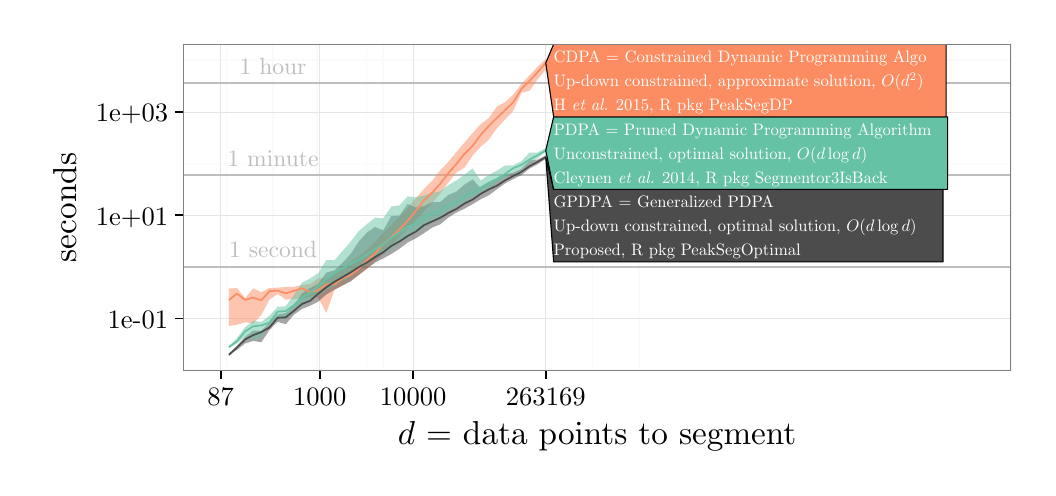
\begin{tikzpicture}[x=1pt,y=1pt]
\definecolor{fillColor}{RGB}{255,255,255}
\path[use as bounding box,fill=fillColor,fill opacity=0.00] (0,0) rectangle (361.35,158.99);
\begin{scope}
\path[clip] (  0.00,  0.00) rectangle (361.35,158.99);
\definecolor{drawColor}{RGB}{255,255,255}
\definecolor{fillColor}{RGB}{255,255,255}

\path[draw=drawColor,line width= 0.6pt,line join=round,line cap=round,fill=fillColor] (  0.00,  0.00) rectangle (361.35,158.99);
\end{scope}
\begin{scope}
\path[clip] ( 56.16, 35.02) rectangle (355.35,152.99);
\definecolor{fillColor}{RGB}{255,255,255}

\path[fill=fillColor] ( 56.16, 35.02) rectangle (355.35,152.99);
\definecolor{drawColor}{gray}{0.98}

\path[draw=drawColor,line width= 0.6pt,line join=round] ( 56.16, 35.18) --
	(355.35, 35.18);

\path[draw=drawColor,line width= 0.6pt,line join=round] ( 56.16, 72.54) --
	(355.35, 72.54);

\path[draw=drawColor,line width= 0.6pt,line join=round] ( 56.16,109.90) --
	(355.35,109.90);

\path[draw=drawColor,line width= 0.6pt,line join=round] ( 56.16,147.26) --
	(355.35,147.26);

\path[draw=drawColor,line width= 0.6pt,line join=round] ( 71.80, 35.02) --
	( 71.80,152.99);

\path[draw=drawColor,line width= 0.6pt,line join=round] ( 88.67, 35.02) --
	( 88.67,152.99);

\path[draw=drawColor,line width= 0.6pt,line join=round] (122.41, 35.02) --
	(122.41,152.99);

\path[draw=drawColor,line width= 0.6pt,line join=round] (104.52, 35.02) --
	(104.52,152.99);

\path[draw=drawColor,line width= 0.6pt,line join=round] (128.48, 35.02) --
	(128.48,152.99);

\path[draw=drawColor,line width= 0.6pt,line join=round] (204.08, 35.02) --
	(204.08,152.99);

\path[draw=drawColor,line width= 0.6pt,line join=round] (220.95, 35.02) --
	(220.95,152.99);
\definecolor{drawColor}{gray}{0.90}

\path[draw=drawColor,line width= 0.2pt,line join=round] ( 56.16, 53.86) --
	(355.35, 53.86);

\path[draw=drawColor,line width= 0.2pt,line join=round] ( 56.16, 91.22) --
	(355.35, 91.22);

\path[draw=drawColor,line width= 0.2pt,line join=round] ( 56.16,128.58) --
	(355.35,128.58);

\path[draw=drawColor,line width= 0.2pt,line join=round] (105.54, 35.02) --
	(105.54,152.99);

\path[draw=drawColor,line width= 0.2pt,line join=round] (139.29, 35.02) --
	(139.29,152.99);

\path[draw=drawColor,line width= 0.2pt,line join=round] ( 69.76, 35.02) --
	( 69.76,152.99);

\path[draw=drawColor,line width= 0.2pt,line join=round] (187.21, 35.02) --
	(187.21,152.99);
\definecolor{drawColor}{RGB}{190,190,190}

\path[draw=drawColor,line width= 0.6pt,line join=round] ( 56.16, 72.54) -- (355.35, 72.54);

\path[draw=drawColor,line width= 0.6pt,line join=round] ( 56.16,105.76) -- (355.35,105.76);

\path[draw=drawColor,line width= 0.6pt,line join=round] ( 56.16,138.97) -- (355.35,138.97);
\definecolor{fillColor}{RGB}{252,141,98}

\path[fill=fillColor,fill opacity=0.50] ( 72.69, 64.75) --
	( 75.63, 64.88) --
	( 78.57, 61.26) --
	( 81.50, 64.77) --
	( 84.44, 63.42) --
	( 87.37, 64.92) --
	( 90.31, 65.04) --
	( 93.25, 65.27) --
	( 96.18, 65.35) --
	( 99.12, 66.06) --
	(102.06, 66.36) --
	(104.99, 68.37) --
	(107.93, 68.61) --
	(110.87, 69.89) --
	(113.80, 72.07) --
	(116.74, 74.38) --
	(119.67, 76.35) --
	(122.61, 78.71) --
	(125.55, 81.73) --
	(128.48, 84.79) --
	(131.42, 87.64) --
	(134.36, 90.64) --
	(137.29, 93.80) --
	(140.23, 97.33) --
	(143.17,100.67) --
	(146.10,103.62) --
	(149.04,107.39) --
	(151.97,110.44) --
	(154.91,114.04) --
	(157.85,117.49) --
	(160.78,120.89) --
	(163.72,124.18) --
	(166.66,126.34) --
	(169.59,130.56) --
	(172.53,132.06) --
	(175.47,134.83) --
	(178.40,138.63) --
	(181.34,141.77) --
	(184.27,144.86) --
	(187.21,147.63) --
	(187.21,143.83) --
	(184.27,140.35) --
	(181.34,136.18) --
	(178.40,135.48) --
	(175.47,128.91) --
	(172.53,125.85) --
	(169.59,122.66) --
	(166.66,118.55) --
	(163.72,115.99) --
	(160.78,112.81) --
	(157.85,108.39) --
	(154.91,106.66) --
	(151.97,102.93) --
	(149.04, 98.99) --
	(146.10, 95.75) --
	(143.17, 92.53) --
	(140.23, 89.28) --
	(137.29, 86.25) --
	(134.36, 83.24) --
	(131.42, 80.34) --
	(128.48, 77.26) --
	(125.55, 74.54) --
	(122.61, 71.80) --
	(119.67, 69.55) --
	(116.74, 67.69) --
	(113.80, 65.75) --
	(110.87, 64.25) --
	(107.93, 55.92) --
	(104.99, 61.45) --
	(102.06, 61.77) --
	( 99.12, 61.10) --
	( 96.18, 60.86) --
	( 93.25, 60.72) --
	( 90.31, 62.77) --
	( 87.37, 60.72) --
	( 84.44, 55.20) --
	( 81.50, 52.05) --
	( 78.57, 52.54) --
	( 75.63, 51.63) --
	( 72.69, 51.19) --
	cycle;
\definecolor{fillColor}{RGB}{77,77,77}

\path[fill=fillColor,fill opacity=0.50] ( 72.69, 41.20) --
	( 75.63, 44.09) --
	( 78.57, 47.20) --
	( 81.50, 49.58) --
	( 84.44, 49.44) --
	( 87.37, 52.35) --
	( 90.31, 55.34) --
	( 93.25, 55.86) --
	( 96.18, 58.49) --
	( 99.12, 62.96) --
	(102.06, 64.88) --
	(104.99, 66.41) --
	(107.93, 70.47) --
	(110.87, 71.30) --
	(113.80, 74.04) --
	(116.74, 77.26) --
	(119.67, 81.73) --
	(122.61, 84.98) --
	(125.55, 86.97) --
	(128.48, 85.74) --
	(131.42, 90.94) --
	(134.36, 91.07) --
	(137.29, 95.25) --
	(140.23, 94.02) --
	(143.17, 94.48) --
	(146.10, 95.92) --
	(149.04, 95.94) --
	(151.97, 98.56) --
	(154.91, 99.73) --
	(157.85,102.31) --
	(160.78,104.17) --
	(163.72,100.94) --
	(166.66,102.79) --
	(169.59,104.47) --
	(172.53,105.95) --
	(175.47,106.60) --
	(178.40,107.96) --
	(181.34,110.98) --
	(184.27,111.34) --
	(187.21,112.86) --
	(187.21,111.62) --
	(184.27,109.63) --
	(181.34,108.05) --
	(178.40,105.71) --
	(175.47,104.31) --
	(172.53,102.71) --
	(169.59,100.66) --
	(166.66, 98.42) --
	(163.72, 97.00) --
	(160.78, 95.21) --
	(157.85, 93.58) --
	(154.91, 92.18) --
	(151.97, 90.33) --
	(149.04, 87.91) --
	(146.10, 86.72) --
	(143.17, 84.69) --
	(140.23, 82.85) --
	(137.29, 81.34) --
	(134.36, 79.11) --
	(131.42, 77.21) --
	(128.48, 75.62) --
	(125.55, 74.09) --
	(122.61, 71.98) --
	(119.67, 69.73) --
	(116.74, 67.28) --
	(113.80, 65.90) --
	(110.87, 64.32) --
	(107.93, 62.58) --
	(104.99, 59.99) --
	(102.06, 58.49) --
	( 99.12, 57.36) --
	( 96.18, 55.27) --
	( 93.25, 51.84) --
	( 90.31, 52.73) --
	( 87.37, 49.71) --
	( 84.44, 45.34) --
	( 81.50, 45.79) --
	( 78.57, 44.86) --
	( 75.63, 42.61) --
	( 72.69, 40.39) --
	cycle;
\definecolor{fillColor}{RGB}{102,194,165}

\path[fill=fillColor,fill opacity=0.50] ( 72.69, 43.82) --
	( 75.63, 46.82) --
	( 78.57, 50.73) --
	( 81.50, 53.09) --
	( 84.44, 52.64) --
	( 87.37, 54.92) --
	( 90.31, 58.12) --
	( 93.25, 58.35) --
	( 96.18, 62.36) --
	( 99.12, 66.88) --
	(102.06, 68.37) --
	(104.99, 70.27) --
	(107.93, 75.02) --
	(110.87, 74.94) --
	(113.80, 78.32) --
	(116.74, 81.66) --
	(119.67, 85.48) --
	(122.61, 88.03) --
	(125.55, 90.36) --
	(128.48, 90.06) --
	(131.42, 94.37) --
	(134.36, 94.79) --
	(137.29, 98.01) --
	(140.23, 97.69) --
	(143.17, 98.32) --
	(146.10, 99.35) --
	(149.04, 99.85) --
	(151.97,102.05) --
	(154.91,103.76) --
	(157.85,105.89) --
	(160.78,108.16) --
	(163.72,103.76) --
	(166.66,105.78) --
	(169.59,107.34) --
	(172.53,109.20) --
	(175.47,109.22) --
	(178.40,110.71) --
	(181.34,113.86) --
	(184.27,113.88) --
	(187.21,115.46) --
	(187.21,114.10) --
	(184.27,111.82) --
	(181.34,110.11) --
	(178.40,107.54) --
	(175.47,106.44) --
	(172.53,104.78) --
	(169.59,103.02) --
	(166.66,100.45) --
	(163.72, 98.81) --
	(160.78, 97.42) --
	(157.85, 95.64) --
	(154.91, 94.34) --
	(151.97, 92.35) --
	(149.04, 89.68) --
	(146.10, 88.73) --
	(143.17, 86.64) --
	(140.23, 84.88) --
	(137.29, 83.01) --
	(134.36, 81.41) --
	(131.42, 78.81) --
	(128.48, 77.31) --
	(125.55, 76.02) --
	(122.61, 73.52) --
	(119.67, 71.88) --
	(116.74, 69.11) --
	(113.80, 67.51) --
	(110.87, 65.69) --
	(107.93, 64.30) --
	(104.99, 62.10) --
	(102.06, 61.00) --
	( 99.12, 58.35) --
	( 96.18, 57.36) --
	( 93.25, 54.02) --
	( 90.31, 54.10) --
	( 87.37, 51.84) --
	( 84.44, 47.20) --
	( 81.50, 46.22) --
	( 78.57, 47.20) --
	( 75.63, 44.86) --
	( 72.69, 43.24) --
	cycle;
\definecolor{drawColor}{RGB}{252,141,98}

\path[draw=drawColor,line width= 0.6pt,line join=round] ( 72.69, 60.53) --
	( 75.63, 62.89) --
	( 78.57, 60.62) --
	( 81.50, 61.45) --
	( 84.44, 60.47) --
	( 87.37, 63.79) --
	( 90.31, 63.99) --
	( 93.25, 62.99) --
	( 96.18, 63.86) --
	( 99.12, 64.82) --
	(102.06, 63.36) --
	(104.99, 64.18) --
	(107.93, 66.19) --
	(110.87, 66.28) --
	(113.80, 68.46) --
	(116.74, 69.66) --
	(119.67, 71.88) --
	(122.61, 74.98) --
	(125.55, 77.38) --
	(128.48, 80.83) --
	(131.42, 83.28) --
	(134.36, 86.10) --
	(137.29, 89.19) --
	(140.23, 92.74) --
	(143.17, 96.57) --
	(146.10, 99.29) --
	(149.04,102.58) --
	(151.97,106.34) --
	(154.91,109.75) --
	(157.85,113.42) --
	(160.78,116.26) --
	(163.72,120.29) --
	(166.66,123.51) --
	(169.59,126.42) --
	(172.53,129.17) --
	(175.47,132.04) --
	(178.40,136.86) --
	(181.34,139.75) --
	(184.27,142.95) --
	(187.21,146.24);
\definecolor{drawColor}{gray}{0.30}

\path[draw=drawColor,line width= 0.6pt,line join=round] ( 72.69, 40.80) --
	( 75.63, 43.39) --
	( 78.57, 46.32) --
	( 81.50, 47.90) --
	( 84.44, 49.01) --
	( 87.37, 50.67) --
	( 90.31, 54.14) --
	( 93.25, 54.33) --
	( 96.18, 56.65) --
	( 99.12, 59.15) --
	(102.06, 60.29) --
	(104.99, 62.84) --
	(107.93, 65.19) --
	(110.87, 67.16) --
	(113.80, 68.86) --
	(116.74, 70.60) --
	(119.67, 72.49) --
	(122.61, 74.13) --
	(125.55, 76.10) --
	(128.48, 77.84) --
	(131.42, 80.13) --
	(134.36, 81.75) --
	(137.29, 83.70) --
	(140.23, 85.28) --
	(143.17, 87.61) --
	(146.10, 88.94) --
	(149.04, 90.27) --
	(151.97, 92.02) --
	(154.91, 93.47) --
	(157.85, 95.45) --
	(160.78, 96.87) --
	(163.72, 98.94) --
	(166.66,100.57) --
	(169.59,101.91) --
	(172.53,103.85) --
	(175.47,105.37) --
	(178.40,106.89) --
	(181.34,108.96) --
	(184.27,110.50) --
	(187.21,112.23);
\definecolor{drawColor}{RGB}{102,194,165}

\path[draw=drawColor,line width= 0.6pt,line join=round] ( 72.69, 43.53) --
	( 75.63, 45.68) --
	( 78.57, 49.23) --
	( 81.50, 51.08) --
	( 84.44, 51.42) --
	( 87.37, 52.40) --
	( 90.31, 56.35) --
	( 93.25, 56.59) --
	( 96.18, 58.72) --
	( 99.12, 61.52) --
	(102.06, 63.13) --
	(104.99, 65.59) --
	(107.93, 68.29) --
	(110.87, 70.41) --
	(113.80, 71.97) --
	(116.74, 73.69) --
	(119.67, 75.18) --
	(122.61, 77.05) --
	(125.55, 78.96) --
	(128.48, 80.67) --
	(131.42, 83.16) --
	(134.36, 85.02) --
	(137.29, 86.88) --
	(140.23, 88.29) --
	(143.17, 90.54) --
	(146.10, 91.81) --
	(149.04, 92.87) --
	(151.97, 94.66) --
	(154.91, 95.97) --
	(157.85, 98.01) --
	(160.78, 99.40) --
	(163.72,101.20) --
	(166.66,102.97) --
	(169.59,104.35) --
	(172.53,106.15) --
	(175.47,108.23) --
	(178.40,109.43) --
	(181.34,111.32) --
	(184.27,112.92) --
	(187.21,114.61);
\definecolor{drawColor}{RGB}{190,190,190}

\node[text=drawColor,anchor=base,inner sep=0pt, outer sep=0pt, scale=  0.85] at ( 88.67, 75.78) {1 second};

\node[text=drawColor,anchor=base,inner sep=0pt, outer sep=0pt, scale=  0.85] at ( 88.67,109.00) {1 minute};

\node[text=drawColor,anchor=base,inner sep=0pt, outer sep=0pt, scale=  0.85] at ( 88.67,142.22) {1 hour};
\end{scope}
\begin{scope}
\path[clip] ( 56.16, 35.02) rectangle (355.35,152.99);
\definecolor{drawColor}{RGB}{0,0,0}
\definecolor{fillColor}{gray}{0.30}

\path[draw=drawColor,line width= 0.4pt,line join=round,line cap=round,fill=fillColor] (187.21,112.23) --
	(190.06,100.57) --
	(330.74,100.57) --
	(330.74, 74.36) --
	(190.06, 74.36) --
	cycle;
\definecolor{fillColor}{RGB}{102,194,165}

\path[draw=drawColor,line width= 0.4pt,line join=round,line cap=round,fill=fillColor] (187.21,114.61) --
	(190.06,126.78) --
	(332.41,126.78) --
	(332.41,100.57) --
	(190.06,100.57) --
	cycle;
\definecolor{fillColor}{RGB}{252,141,98}

\path[draw=drawColor,line width= 0.4pt,line join=round,line cap=round,fill=fillColor] (187.21,146.24) --
	(190.06,152.99) --
	(331.88,152.99) --
	(331.88,126.78) --
	(190.06,126.78) --
	cycle;
\definecolor{drawColor}{RGB}{255,255,255}

\node[text=drawColor,anchor=base west,inner sep=0pt, outer sep=0pt, scale=  0.60] at (190.06, 93.83) {GPDPA = Generalized PDPA};

\node[text=drawColor,anchor=base west,inner sep=0pt, outer sep=0pt, scale=  0.60] at (190.06, 85.19) {Up-down constrained, optimal solution, $O(d \log d)$};

\node[text=drawColor,anchor=base west,inner sep=0pt, outer sep=0pt, scale=  0.60] at (190.06, 76.55) {Proposed, R pkg PeakSegOptimal};

\node[text=drawColor,anchor=base west,inner sep=0pt, outer sep=0pt, scale=  0.60] at (190.06,120.04) {PDPA = Pruned Dynamic Programming Algorithm};

\node[text=drawColor,anchor=base west,inner sep=0pt, outer sep=0pt, scale=  0.60] at (190.06,111.40) {Unconstrained, optimal solution, $O(d \log d)$};

\node[text=drawColor,anchor=base west,inner sep=0pt, outer sep=0pt, scale=  0.60] at (190.06,102.76) {Cleynen {\it et al.} 2014, R pkg Segmentor3IsBack};

\node[text=drawColor,anchor=base west,inner sep=0pt, outer sep=0pt, scale=  0.60] at (190.06,146.25) {CDPA = Constrained Dynamic Programming Algo};

\node[text=drawColor,anchor=base west,inner sep=0pt, outer sep=0pt, scale=  0.60] at (190.06,137.61) {Up-down constrained, approximate solution, $O(d^2)$};

\node[text=drawColor,anchor=base west,inner sep=0pt, outer sep=0pt, scale=  0.60] at (190.06,128.97) {H {\it et al.} 2015, R pkg PeakSegDP};
\definecolor{drawColor}{gray}{0.50}

\path[draw=drawColor,line width= 0.6pt,line join=round,line cap=round] ( 56.16, 35.02) rectangle (355.35,152.99);
\end{scope}
\begin{scope}
\path[clip] (  0.00,  0.00) rectangle (361.35,158.99);
\definecolor{drawColor}{RGB}{0,0,0}

\node[text=drawColor,anchor=base east,inner sep=0pt, outer sep=0pt, scale=  0.96] at ( 50.76, 50.21) {1e-01};

\node[text=drawColor,anchor=base east,inner sep=0pt, outer sep=0pt, scale=  0.96] at ( 50.76, 87.57) {1e+01};

\node[text=drawColor,anchor=base east,inner sep=0pt, outer sep=0pt, scale=  0.96] at ( 50.76,124.93) {1e+03};
\end{scope}
\begin{scope}
\path[clip] (  0.00,  0.00) rectangle (361.35,158.99);
\definecolor{drawColor}{RGB}{0,0,0}

\path[draw=drawColor,line width= 0.6pt,line join=round] ( 53.16, 53.86) --
	( 56.16, 53.86);

\path[draw=drawColor,line width= 0.6pt,line join=round] ( 53.16, 91.22) --
	( 56.16, 91.22);

\path[draw=drawColor,line width= 0.6pt,line join=round] ( 53.16,128.58) --
	( 56.16,128.58);
\end{scope}
\begin{scope}
\path[clip] (  0.00,  0.00) rectangle (361.35,158.99);
\definecolor{drawColor}{RGB}{0,0,0}

\path[draw=drawColor,line width= 0.6pt,line join=round] (105.54, 32.02) --
	(105.54, 35.02);

\path[draw=drawColor,line width= 0.6pt,line join=round] (139.29, 32.02) --
	(139.29, 35.02);

\path[draw=drawColor,line width= 0.6pt,line join=round] ( 69.76, 32.02) --
	( 69.76, 35.02);

\path[draw=drawColor,line width= 0.6pt,line join=round] (187.21, 32.02) --
	(187.21, 35.02);
\end{scope}
\begin{scope}
\path[clip] (  0.00,  0.00) rectangle (361.35,158.99);
\definecolor{drawColor}{RGB}{0,0,0}

\node[text=drawColor,anchor=base,inner sep=0pt, outer sep=0pt, scale=  0.96] at (105.54, 22.32) {1000};

\node[text=drawColor,anchor=base,inner sep=0pt, outer sep=0pt, scale=  0.96] at (139.29, 22.32) {10000};

\node[text=drawColor,anchor=base,inner sep=0pt, outer sep=0pt, scale=  0.96] at ( 69.76, 22.32) {87};

\node[text=drawColor,anchor=base,inner sep=0pt, outer sep=0pt, scale=  0.96] at (187.21, 22.32) {263169};
\end{scope}
\begin{scope}
\path[clip] (  0.00,  0.00) rectangle (361.35,158.99);
\definecolor{drawColor}{RGB}{0,0,0}

\node[text=drawColor,anchor=base,inner sep=0pt, outer sep=0pt, scale=  1.20] at (205.75,  8.40) {$d$ = data points to segment};
\end{scope}
\begin{scope}
\path[clip] (  0.00,  0.00) rectangle (361.35,158.99);
\definecolor{drawColor}{RGB}{0,0,0}

\node[text=drawColor,rotate= 90.00,anchor=base,inner sep=0pt, outer sep=0pt, scale=  1.20] at ( 17.52, 94.01) {seconds};
\end{scope}
\end{tikzpicture}


  % \hskip -1cm
  % \parbox{0.53\textwidth}{
  %   % Created by tikzDevice version 0.10.1 on 2017-06-15 12:55:53
% !TEX encoding = UTF-8 Unicode
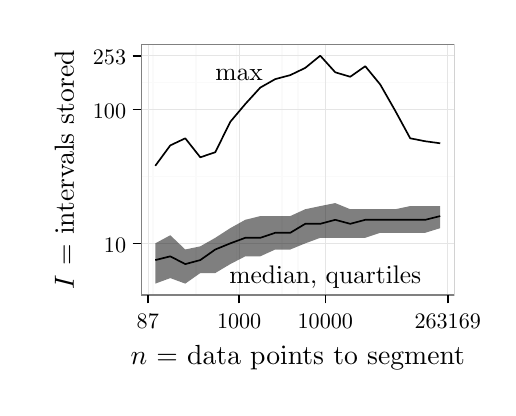
\begin{tikzpicture}[x=1pt,y=1pt]
\definecolor{fillColor}{RGB}{255,255,255}
\path[use as bounding box,fill=fillColor,fill opacity=0.00] (0,0) rectangle (166.22,130.09);
\begin{scope}
\path[clip] (  0.00,  0.00) rectangle (166.22,130.09);
\definecolor{drawColor}{RGB}{255,255,255}
\definecolor{fillColor}{RGB}{255,255,255}

\path[draw=drawColor,line width= 0.6pt,line join=round,line cap=round,fill=fillColor] (  0.00,  0.00) rectangle (166.22,130.09);
\end{scope}
\begin{scope}
\path[clip] ( 40.96, 33.48) rectangle (154.22,124.09);
\definecolor{fillColor}{RGB}{255,255,255}

\path[fill=fillColor] ( 40.96, 33.48) rectangle (154.22,124.09);
\definecolor{drawColor}{gray}{0.98}

\path[draw=drawColor,line width= 0.6pt,line join=round] ( 40.96, 76.31) --
	(154.22, 76.31);

\path[draw=drawColor,line width= 0.6pt,line join=round] ( 40.96,110.22) --
	(154.22,110.22);

\path[draw=drawColor,line width= 0.6pt,line join=round] ( 45.28, 33.48) --
	( 45.28,124.09);

\path[draw=drawColor,line width= 0.6pt,line join=round] ( 60.85, 33.48) --
	( 60.85,124.09);

\path[draw=drawColor,line width= 0.6pt,line join=round] ( 91.99, 33.48) --
	( 91.99,124.09);

\path[draw=drawColor,line width= 0.6pt,line join=round] ( 75.48, 33.48) --
	( 75.48,124.09);

\path[draw=drawColor,line width= 0.6pt,line join=round] ( 97.59, 33.48) --
	( 97.59,124.09);
\definecolor{drawColor}{gray}{0.90}

\path[draw=drawColor,line width= 0.2pt,line join=round] ( 40.96, 52.15) --
	(154.22, 52.15);

\path[draw=drawColor,line width= 0.2pt,line join=round] ( 40.96,100.48) --
	(154.22,100.48);

\path[draw=drawColor,line width= 0.2pt,line join=round] ( 40.96,119.97) --
	(154.22,119.97);

\path[draw=drawColor,line width= 0.2pt,line join=round] ( 76.42, 33.48) --
	( 76.42,124.09);

\path[draw=drawColor,line width= 0.2pt,line join=round] (107.56, 33.48) --
	(107.56,124.09);

\path[draw=drawColor,line width= 0.2pt,line join=round] ( 43.40, 33.48) --
	( 43.40,124.09);

\path[draw=drawColor,line width= 0.2pt,line join=round] (151.78, 33.48) --
	(151.78,124.09);
\definecolor{drawColor}{RGB}{0,0,0}

\node[text=drawColor,anchor=base,inner sep=0pt, outer sep=0pt, scale=  0.92] at ( 76.42,111.18) {max};

\node[text=drawColor,anchor=base,inner sep=0pt, outer sep=0pt, scale=  0.92] at (107.56, 37.62) {median, quartiles};

\path[draw=drawColor,line width= 0.6pt,line join=round] ( 46.11, 80.17) --
	( 51.53, 87.55) --
	( 56.95, 90.11) --
	( 62.37, 83.25) --
	( 67.79, 85.07) --
	( 73.21, 96.06) --
	( 78.62,102.48) --
	( 84.04,108.43) --
	( 89.46,111.50) --
	( 94.88,112.94) --
	(100.30,115.55) --
	(105.72,119.97) --
	(111.14,113.96) --
	(116.56,112.35) --
	(121.98,116.16) --
	(127.40,109.55) --
	(132.82,100.06) --
	(138.23, 90.11) --
	(143.65, 89.05) --
	(149.07, 88.31);
\definecolor{fillColor}{RGB}{0,0,0}

\path[fill=fillColor,fill opacity=0.50] ( 46.11, 52.15) --
	( 51.53, 55.08) --
	( 56.95, 49.93) --
	( 62.37, 51.07) --
	( 67.79, 54.15) --
	( 73.21, 57.65) --
	( 78.62, 60.66) --
	( 84.04, 62.01) --
	( 89.46, 62.01) --
	( 94.88, 62.01) --
	(100.30, 64.48) --
	(105.72, 65.62) --
	(111.14, 66.70) --
	(116.56, 64.48) --
	(121.98, 64.48) --
	(127.40, 64.48) --
	(132.82, 64.48) --
	(138.23, 65.62) --
	(143.65, 65.62) --
	(149.07, 65.62) --
	(149.07, 57.65) --
	(143.65, 55.97) --
	(138.23, 55.97) --
	(132.82, 55.97) --
	(127.40, 55.97) --
	(121.98, 54.15) --
	(116.56, 54.15) --
	(111.14, 54.15) --
	(105.72, 54.15) --
	(100.30, 52.15) --
	( 94.88, 49.93) --
	( 89.46, 49.93) --
	( 84.04, 47.46) --
	( 78.62, 47.46) --
	( 73.21, 44.66) --
	( 67.79, 41.42) --
	( 62.37, 41.42) --
	( 56.95, 37.60) --
	( 51.53, 39.60) --
	( 46.11, 37.60) --
	cycle;

\path[draw=drawColor,line width= 0.6pt,line join=round] ( 46.11, 46.11) --
	( 51.53, 47.46) --
	( 56.95, 44.66) --
	( 62.37, 46.11) --
	( 67.79, 49.93) --
	( 73.21, 52.15) --
	( 78.62, 54.15) --
	( 84.04, 54.15) --
	( 89.46, 55.97) --
	( 94.88, 55.97) --
	(100.30, 59.21) --
	(105.72, 59.21) --
	(111.14, 60.66) --
	(116.56, 59.21) --
	(121.98, 60.66) --
	(127.40, 60.66) --
	(132.82, 60.66) --
	(138.23, 60.66) --
	(143.65, 60.66) --
	(149.07, 62.01);
\definecolor{drawColor}{gray}{0.50}

\path[draw=drawColor,line width= 0.6pt,line join=round,line cap=round] ( 40.96, 33.48) rectangle (154.22,124.09);
\end{scope}
\begin{scope}
\path[clip] (  0.00,  0.00) rectangle (166.22,130.09);
\definecolor{drawColor}{RGB}{0,0,0}

\node[text=drawColor,anchor=base east,inner sep=0pt, outer sep=0pt, scale=  0.80] at ( 35.56, 48.84) {10};

\node[text=drawColor,anchor=base east,inner sep=0pt, outer sep=0pt, scale=  0.80] at ( 35.56, 97.18) {100};

\node[text=drawColor,anchor=base east,inner sep=0pt, outer sep=0pt, scale=  0.80] at ( 35.56,116.66) {253};
\end{scope}
\begin{scope}
\path[clip] (  0.00,  0.00) rectangle (166.22,130.09);
\definecolor{drawColor}{RGB}{0,0,0}

\path[draw=drawColor,line width= 0.6pt,line join=round] ( 37.96, 52.15) --
	( 40.96, 52.15);

\path[draw=drawColor,line width= 0.6pt,line join=round] ( 37.96,100.48) --
	( 40.96,100.48);

\path[draw=drawColor,line width= 0.6pt,line join=round] ( 37.96,119.97) --
	( 40.96,119.97);
\end{scope}
\begin{scope}
\path[clip] (  0.00,  0.00) rectangle (166.22,130.09);
\definecolor{drawColor}{RGB}{0,0,0}

\path[draw=drawColor,line width= 0.6pt,line join=round] ( 76.42, 30.48) --
	( 76.42, 33.48);

\path[draw=drawColor,line width= 0.6pt,line join=round] (107.56, 30.48) --
	(107.56, 33.48);

\path[draw=drawColor,line width= 0.6pt,line join=round] ( 43.40, 30.48) --
	( 43.40, 33.48);

\path[draw=drawColor,line width= 0.6pt,line join=round] (151.78, 30.48) --
	(151.78, 33.48);
\end{scope}
\begin{scope}
\path[clip] (  0.00,  0.00) rectangle (166.22,130.09);
\definecolor{drawColor}{RGB}{0,0,0}

\node[text=drawColor,anchor=base,inner sep=0pt, outer sep=0pt, scale=  0.80] at ( 76.42, 21.46) {1000};

\node[text=drawColor,anchor=base,inner sep=0pt, outer sep=0pt, scale=  0.80] at (107.56, 21.46) {10000};

\node[text=drawColor,anchor=base,inner sep=0pt, outer sep=0pt, scale=  0.80] at ( 43.40, 21.46) {87};

\node[text=drawColor,anchor=base,inner sep=0pt, outer sep=0pt, scale=  0.80] at (151.78, 21.46) {263169};
\end{scope}
\begin{scope}
\path[clip] (  0.00,  0.00) rectangle (166.22,130.09);
\definecolor{drawColor}{RGB}{0,0,0}

\node[text=drawColor,anchor=base,inner sep=0pt, outer sep=0pt, scale=  1.00] at ( 97.59,  8.40) {$n$ = data points to segment};
\end{scope}
\begin{scope}
\path[clip] (  0.00,  0.00) rectangle (166.22,130.09);
\definecolor{drawColor}{RGB}{0,0,0}

\node[text=drawColor,rotate= 90.00,anchor=base,inner sep=0pt, outer sep=0pt, scale=  1.00] at ( 16.66, 78.78) {$I$ = intervals stored};
\end{scope}
\end{tikzpicture}

  % }
  % \parbox{0.49\textwidth}{
  %   % Created by tikzDevice version 0.10.1 on 2017-07-31 15:48:42
% !TEX encoding = UTF-8 Unicode
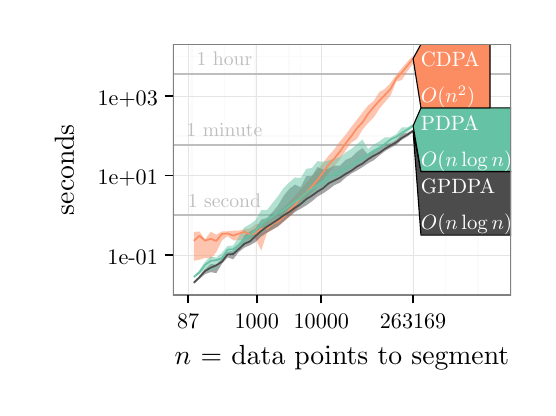
\begin{tikzpicture}[x=1pt,y=1pt]
\definecolor{fillColor}{RGB}{255,255,255}
\path[use as bounding box,fill=fillColor,fill opacity=0.00] (0,0) rectangle (180.67,130.09);
\begin{scope}
\path[clip] (  0.00,  0.00) rectangle (180.67,130.09);
\definecolor{drawColor}{RGB}{255,255,255}
\definecolor{fillColor}{RGB}{255,255,255}

\path[draw=drawColor,line width= 0.6pt,line join=round,line cap=round,fill=fillColor] (  0.00,  0.00) rectangle (180.68,130.09);
\end{scope}
\begin{scope}
\path[clip] ( 52.45, 33.48) rectangle (174.67,124.09);
\definecolor{fillColor}{RGB}{255,255,255}

\path[fill=fillColor] ( 52.45, 33.48) rectangle (174.67,124.09);
\definecolor{drawColor}{gray}{0.98}

\path[draw=drawColor,line width= 0.6pt,line join=round] ( 52.45, 33.60) --
	(174.67, 33.60);

\path[draw=drawColor,line width= 0.6pt,line join=round] ( 52.45, 62.29) --
	(174.67, 62.29);

\path[draw=drawColor,line width= 0.6pt,line join=round] ( 52.45, 90.99) --
	(174.67, 90.99);

\path[draw=drawColor,line width= 0.6pt,line join=round] ( 52.45,119.68) --
	(174.67,119.68);

\path[draw=drawColor,line width= 0.6pt,line join=round] ( 59.42, 33.48) --
	( 59.42,124.09);

\path[draw=drawColor,line width= 0.6pt,line join=round] ( 71.09, 33.48) --
	( 71.09,124.09);

\path[draw=drawColor,line width= 0.6pt,line join=round] ( 94.43, 33.48) --
	( 94.43,124.09);

\path[draw=drawColor,line width= 0.6pt,line join=round] ( 82.06, 33.48) --
	( 82.06,124.09);

\path[draw=drawColor,line width= 0.6pt,line join=round] ( 98.63, 33.48) --
	( 98.63,124.09);

\path[draw=drawColor,line width= 0.6pt,line join=round] (150.94, 33.48) --
	(150.94,124.09);

\path[draw=drawColor,line width= 0.6pt,line join=round] (162.61, 33.48) --
	(162.61,124.09);
\definecolor{drawColor}{gray}{0.90}

\path[draw=drawColor,line width= 0.2pt,line join=round] ( 52.45, 47.94) --
	(174.67, 47.94);

\path[draw=drawColor,line width= 0.2pt,line join=round] ( 52.45, 76.64) --
	(174.67, 76.64);

\path[draw=drawColor,line width= 0.2pt,line join=round] ( 52.45,105.34) --
	(174.67,105.34);

\path[draw=drawColor,line width= 0.2pt,line join=round] ( 82.76, 33.48) --
	( 82.76,124.09);

\path[draw=drawColor,line width= 0.2pt,line join=round] (106.11, 33.48) --
	(106.11,124.09);

\path[draw=drawColor,line width= 0.2pt,line join=round] ( 58.00, 33.48) --
	( 58.00,124.09);

\path[draw=drawColor,line width= 0.2pt,line join=round] (139.27, 33.48) --
	(139.27,124.09);
\definecolor{drawColor}{RGB}{190,190,190}

\path[draw=drawColor,line width= 0.6pt,line join=round] ( 52.45, 62.29) -- (174.67, 62.29);

\path[draw=drawColor,line width= 0.6pt,line join=round] ( 52.45, 87.80) -- (174.67, 87.80);

\path[draw=drawColor,line width= 0.6pt,line join=round] ( 52.45,113.32) -- (174.67,113.32);
\definecolor{fillColor}{RGB}{252,141,98}

\path[fill=fillColor,fill opacity=0.50] ( 60.03, 56.31) --
	( 62.07, 56.41) --
	( 64.10, 53.63) --
	( 66.13, 56.33) --
	( 68.16, 55.29) --
	( 70.19, 56.44) --
	( 72.22, 56.53) --
	( 74.26, 56.71) --
	( 76.29, 56.77) --
	( 78.32, 57.32) --
	( 80.35, 57.55) --
	( 82.38, 59.09) --
	( 84.41, 59.27) --
	( 86.44, 60.25) --
	( 88.48, 61.93) --
	( 90.51, 63.71) --
	( 92.54, 65.22) --
	( 94.57, 67.03) --
	( 96.60, 69.35) --
	( 98.63, 71.70) --
	(100.67, 73.89) --
	(102.70, 76.20) --
	(104.73, 78.62) --
	(106.76, 81.34) --
	(108.79, 83.90) --
	(110.82, 86.17) --
	(112.86, 89.06) --
	(114.89, 91.40) --
	(116.92, 94.17) --
	(118.95, 96.82) --
	(120.98, 99.43) --
	(123.01,101.96) --
	(125.04,103.61) --
	(127.08,106.85) --
	(129.11,108.01) --
	(131.14,110.14) --
	(133.17,113.05) --
	(135.20,115.46) --
	(137.23,117.84) --
	(139.27,119.97) --
	(139.27,117.05) --
	(137.23,114.38) --
	(135.20,111.17) --
	(133.17,110.63) --
	(131.14,105.59) --
	(129.11,103.24) --
	(127.08,100.79) --
	(125.04, 97.63) --
	(123.01, 95.66) --
	(120.98, 93.22) --
	(118.95, 89.83) --
	(116.92, 88.50) --
	(114.89, 85.63) --
	(112.86, 82.61) --
	(110.82, 80.12) --
	(108.79, 77.65) --
	(106.76, 75.15) --
	(104.73, 72.82) --
	(102.70, 70.51) --
	(100.67, 68.28) --
	( 98.63, 65.92) --
	( 96.60, 63.83) --
	( 94.57, 61.72) --
	( 92.54, 60.00) --
	( 90.51, 58.57) --
	( 88.48, 57.08) --
	( 86.44, 55.93) --
	( 84.41, 49.53) --
	( 82.38, 53.78) --
	( 80.35, 54.02) --
	( 78.32, 53.50) --
	( 76.29, 53.32) --
	( 74.26, 53.21) --
	( 72.22, 54.79) --
	( 70.19, 53.21) --
	( 68.16, 48.97) --
	( 66.13, 46.55) --
	( 64.10, 46.93) --
	( 62.07, 46.23) --
	( 60.03, 45.90) --
	cycle;
\definecolor{fillColor}{RGB}{77,77,77}

\path[fill=fillColor,fill opacity=0.50] ( 60.03, 38.22) --
	( 62.07, 40.44) --
	( 64.10, 42.83) --
	( 66.13, 44.66) --
	( 68.16, 44.55) --
	( 70.19, 46.78) --
	( 72.22, 49.08) --
	( 74.26, 49.48) --
	( 76.29, 51.50) --
	( 78.32, 54.93) --
	( 80.35, 56.41) --
	( 82.38, 57.59) --
	( 84.41, 60.70) --
	( 86.44, 61.34) --
	( 88.48, 63.44) --
	( 90.51, 65.92) --
	( 92.54, 69.35) --
	( 94.57, 71.84) --
	( 96.60, 73.37) --
	( 98.63, 72.43) --
	(100.67, 76.42) --
	(102.70, 76.52) --
	(104.73, 79.73) --
	(106.76, 78.79) --
	(108.79, 79.14) --
	(110.82, 80.25) --
	(112.86, 80.26) --
	(114.89, 82.28) --
	(116.92, 83.17) --
	(118.95, 85.16) --
	(120.98, 86.58) --
	(123.01, 84.11) --
	(125.04, 85.53) --
	(127.08, 86.82) --
	(129.11, 87.95) --
	(131.14, 88.45) --
	(133.17, 89.50) --
	(135.20, 91.81) --
	(137.23, 92.09) --
	(139.27, 93.26) --
	(139.27, 92.31) --
	(137.23, 90.78) --
	(135.20, 89.57) --
	(133.17, 87.77) --
	(131.14, 86.69) --
	(129.11, 85.47) --
	(127.08, 83.89) --
	(125.04, 82.17) --
	(123.01, 81.08) --
	(120.98, 79.71) --
	(118.95, 78.46) --
	(116.92, 77.38) --
	(114.89, 75.95) --
	(112.86, 74.09) --
	(110.82, 73.18) --
	(108.79, 71.62) --
	(106.76, 70.21) --
	(104.73, 69.05) --
	(102.70, 67.34) --
	(100.67, 65.88) --
	( 98.63, 64.65) --
	( 96.60, 63.48) --
	( 94.57, 61.86) --
	( 92.54, 60.13) --
	( 90.51, 58.25) --
	( 88.48, 57.19) --
	( 86.44, 55.98) --
	( 84.41, 54.64) --
	( 82.38, 52.66) --
	( 80.35, 51.50) --
	( 78.32, 50.63) --
	( 76.29, 49.03) --
	( 74.26, 46.40) --
	( 72.22, 47.08) --
	( 70.19, 44.76) --
	( 68.16, 41.40) --
	( 66.13, 41.75) --
	( 64.10, 41.04) --
	( 62.07, 39.31) --
	( 60.03, 37.60) --
	cycle;
\definecolor{fillColor}{RGB}{102,194,165}

\path[fill=fillColor,fill opacity=0.50] ( 60.03, 40.23) --
	( 62.07, 42.54) --
	( 64.10, 45.54) --
	( 66.13, 47.36) --
	( 68.16, 47.00) --
	( 70.19, 48.76) --
	( 72.22, 51.21) --
	( 74.26, 51.39) --
	( 76.29, 54.47) --
	( 78.32, 57.95) --
	( 80.35, 59.09) --
	( 82.38, 60.55) --
	( 84.41, 64.19) --
	( 86.44, 64.13) --
	( 88.48, 66.73) --
	( 90.51, 69.29) --
	( 92.54, 72.23) --
	( 94.57, 74.19) --
	( 96.60, 75.98) --
	( 98.63, 75.75) --
	(100.67, 79.06) --
	(102.70, 79.38) --
	(104.73, 81.85) --
	(106.76, 81.61) --
	(108.79, 82.09) --
	(110.82, 82.89) --
	(112.86, 83.27) --
	(114.89, 84.96) --
	(116.92, 86.27) --
	(118.95, 87.91) --
	(120.98, 89.65) --
	(123.01, 86.27) --
	(125.04, 87.83) --
	(127.08, 89.02) --
	(129.11, 90.45) --
	(131.14, 90.47) --
	(133.17, 91.61) --
	(135.20, 94.03) --
	(137.23, 94.05) --
	(139.27, 95.26) --
	(139.27, 94.21) --
	(137.23, 92.46) --
	(135.20, 91.15) --
	(133.17, 89.18) --
	(131.14, 88.33) --
	(129.11, 87.05) --
	(127.08, 85.70) --
	(125.04, 83.73) --
	(123.01, 82.47) --
	(120.98, 81.40) --
	(118.95, 80.04) --
	(116.92, 79.04) --
	(114.89, 77.51) --
	(112.86, 75.46) --
	(110.82, 74.73) --
	(108.79, 73.12) --
	(106.76, 71.77) --
	(104.73, 70.33) --
	(102.70, 69.10) --
	(100.67, 67.11) --
	( 98.63, 65.96) --
	( 96.60, 64.97) --
	( 94.57, 63.04) --
	( 92.54, 61.79) --
	( 90.51, 59.65) --
	( 88.48, 58.43) --
	( 86.44, 57.03) --
	( 84.41, 55.96) --
	( 82.38, 54.27) --
	( 80.35, 53.42) --
	( 78.32, 51.39) --
	( 76.29, 50.63) --
	( 74.26, 48.07) --
	( 72.22, 48.13) --
	( 70.19, 46.40) --
	( 68.16, 42.83) --
	( 66.13, 42.08) --
	( 64.10, 42.83) --
	( 62.07, 41.04) --
	( 60.03, 39.78) --
	cycle;
\definecolor{drawColor}{RGB}{252,141,98}

\path[draw=drawColor,line width= 0.6pt,line join=round] ( 60.03, 53.07) --
	( 62.07, 54.88) --
	( 64.10, 53.13) --
	( 66.13, 53.78) --
	( 68.16, 53.02) --
	( 70.19, 55.57) --
	( 72.22, 55.72) --
	( 74.26, 54.95) --
	( 76.29, 55.62) --
	( 78.32, 56.36) --
	( 80.35, 55.24) --
	( 82.38, 55.87) --
	( 84.41, 57.41) --
	( 86.44, 57.49) --
	( 88.48, 59.16) --
	( 90.51, 60.08) --
	( 92.54, 61.78) --
	( 94.57, 64.16) --
	( 96.60, 66.01) --
	( 98.63, 68.66) --
	(100.67, 70.54) --
	(102.70, 72.71) --
	(104.73, 75.08) --
	(106.76, 77.81) --
	(108.79, 80.75) --
	(110.82, 82.83) --
	(112.86, 85.37) --
	(114.89, 88.25) --
	(116.92, 90.88) --
	(118.95, 93.69) --
	(120.98, 95.87) --
	(123.01, 98.97) --
	(125.04,101.44) --
	(127.08,103.68) --
	(129.11,105.79) --
	(131.14,108.00) --
	(133.17,111.70) --
	(135.20,113.91) --
	(137.23,116.37) --
	(139.27,118.90);
\definecolor{drawColor}{gray}{0.30}

\path[draw=drawColor,line width= 0.6pt,line join=round] ( 60.03, 37.91) --
	( 62.07, 39.90) --
	( 64.10, 42.16) --
	( 66.13, 43.37) --
	( 68.16, 44.22) --
	( 70.19, 45.49) --
	( 72.22, 48.16) --
	( 74.26, 48.31) --
	( 76.29, 50.08) --
	( 78.32, 52.01) --
	( 80.35, 52.88) --
	( 82.38, 54.84) --
	( 84.41, 56.64) --
	( 86.44, 58.16) --
	( 88.48, 59.46) --
	( 90.51, 60.80) --
	( 92.54, 62.26) --
	( 94.57, 63.52) --
	( 96.60, 65.03) --
	( 98.63, 66.36) --
	(100.67, 68.12) --
	(102.70, 69.37) --
	(104.73, 70.86) --
	(106.76, 72.08) --
	(108.79, 73.87) --
	(110.82, 74.89) --
	(112.86, 75.91) --
	(114.89, 77.25) --
	(116.92, 78.37) --
	(118.95, 79.89) --
	(120.98, 80.98) --
	(123.01, 82.57) --
	(125.04, 83.82) --
	(127.08, 84.85) --
	(129.11, 86.34) --
	(131.14, 87.50) --
	(133.17, 88.67) --
	(135.20, 90.26) --
	(137.23, 91.44) --
	(139.27, 92.78);
\definecolor{drawColor}{RGB}{102,194,165}

\path[draw=drawColor,line width= 0.6pt,line join=round] ( 60.03, 40.01) --
	( 62.07, 41.66) --
	( 64.10, 44.39) --
	( 66.13, 45.81) --
	( 68.16, 46.07) --
	( 70.19, 46.82) --
	( 72.22, 49.86) --
	( 74.26, 50.04) --
	( 76.29, 51.67) --
	( 78.32, 53.83) --
	( 80.35, 55.06) --
	( 82.38, 56.95) --
	( 84.41, 59.02) --
	( 86.44, 60.66) --
	( 88.48, 61.85) --
	( 90.51, 63.17) --
	( 92.54, 64.32) --
	( 94.57, 65.76) --
	( 96.60, 67.22) --
	( 98.63, 68.54) --
	(100.67, 70.45) --
	(102.70, 71.88) --
	(104.73, 73.31) --
	(106.76, 74.39) --
	(108.79, 76.12) --
	(110.82, 77.09) --
	(112.86, 77.91) --
	(114.89, 79.28) --
	(116.92, 80.29) --
	(118.95, 81.85) --
	(120.98, 82.92) --
	(123.01, 84.31) --
	(125.04, 85.66) --
	(127.08, 86.72) --
	(129.11, 88.11) --
	(131.14, 89.70) --
	(133.17, 90.62) --
	(135.20, 92.08) --
	(137.23, 93.31) --
	(139.27, 94.60);
\definecolor{drawColor}{RGB}{190,190,190}

\node[text=drawColor,anchor=base,inner sep=0pt, outer sep=0pt, scale=  0.71] at ( 71.09, 65.23) {1 second};

\node[text=drawColor,anchor=base,inner sep=0pt, outer sep=0pt, scale=  0.71] at ( 71.09, 90.74) {1 minute};

\node[text=drawColor,anchor=base,inner sep=0pt, outer sep=0pt, scale=  0.71] at ( 71.09,116.26) {1 hour};
\end{scope}
\begin{scope}
\path[clip] ( 52.45, 33.48) rectangle (174.67,124.09);
\definecolor{drawColor}{RGB}{0,0,0}
\definecolor{fillColor}{gray}{0.30}

\path[draw=drawColor,line width= 0.4pt,line join=round,line cap=round,fill=fillColor] (139.27, 92.78) --
	(142.11, 78.11) --
	(180.67, 78.11) --
	(180.67, 55.12) --
	(142.11, 55.12) --
	cycle;
\definecolor{fillColor}{RGB}{102,194,165}

\path[draw=drawColor,line width= 0.4pt,line join=round,line cap=round,fill=fillColor] (139.27, 94.60) --
	(142.11,101.10) --
	(180.67,101.10) --
	(180.67, 78.11) --
	(142.11, 78.11) --
	cycle;
\definecolor{fillColor}{RGB}{252,141,98}

\path[draw=drawColor,line width= 0.4pt,line join=round,line cap=round,fill=fillColor] (139.27,118.90) --
	(142.11,124.09) --
	(167.07,124.09) --
	(167.07,101.10) --
	(142.11,101.10) --
	cycle;
\definecolor{drawColor}{RGB}{255,255,255}

\node[text=drawColor,anchor=base west,inner sep=0pt, outer sep=0pt, scale=  0.75] at (142.11, 69.99) {GPDPA};

\node[text=drawColor,anchor=base west,inner sep=0pt, outer sep=0pt, scale=  0.75] at (142.11, 57.03) {$O(n \log n)$};

\node[text=drawColor,anchor=base west,inner sep=0pt, outer sep=0pt, scale=  0.75] at (142.11, 92.98) {PDPA};

\node[text=drawColor,anchor=base west,inner sep=0pt, outer sep=0pt, scale=  0.75] at (142.11, 80.02) {$O(n \log n)$};

\node[text=drawColor,anchor=base west,inner sep=0pt, outer sep=0pt, scale=  0.75] at (142.11,115.97) {CDPA};

\node[text=drawColor,anchor=base west,inner sep=0pt, outer sep=0pt, scale=  0.75] at (142.11,103.01) {$O(n^2)$};
\definecolor{drawColor}{gray}{0.50}

\path[draw=drawColor,line width= 0.6pt,line join=round,line cap=round] ( 52.45, 33.48) rectangle (174.67,124.09);
\end{scope}
\begin{scope}
\path[clip] (  0.00,  0.00) rectangle (180.67,130.09);
\definecolor{drawColor}{RGB}{0,0,0}

\node[text=drawColor,anchor=base east,inner sep=0pt, outer sep=0pt, scale=  0.80] at ( 47.05, 44.64) {1e-01};

\node[text=drawColor,anchor=base east,inner sep=0pt, outer sep=0pt, scale=  0.80] at ( 47.05, 73.33) {1e+01};

\node[text=drawColor,anchor=base east,inner sep=0pt, outer sep=0pt, scale=  0.80] at ( 47.05,102.03) {1e+03};
\end{scope}
\begin{scope}
\path[clip] (  0.00,  0.00) rectangle (180.67,130.09);
\definecolor{drawColor}{RGB}{0,0,0}

\path[draw=drawColor,line width= 0.6pt,line join=round] ( 49.45, 47.94) --
	( 52.45, 47.94);

\path[draw=drawColor,line width= 0.6pt,line join=round] ( 49.45, 76.64) --
	( 52.45, 76.64);

\path[draw=drawColor,line width= 0.6pt,line join=round] ( 49.45,105.34) --
	( 52.45,105.34);
\end{scope}
\begin{scope}
\path[clip] (  0.00,  0.00) rectangle (180.67,130.09);
\definecolor{drawColor}{RGB}{0,0,0}

\path[draw=drawColor,line width= 0.6pt,line join=round] ( 82.76, 30.48) --
	( 82.76, 33.48);

\path[draw=drawColor,line width= 0.6pt,line join=round] (106.11, 30.48) --
	(106.11, 33.48);

\path[draw=drawColor,line width= 0.6pt,line join=round] ( 58.00, 30.48) --
	( 58.00, 33.48);

\path[draw=drawColor,line width= 0.6pt,line join=round] (139.27, 30.48) --
	(139.27, 33.48);
\end{scope}
\begin{scope}
\path[clip] (  0.00,  0.00) rectangle (180.67,130.09);
\definecolor{drawColor}{RGB}{0,0,0}

\node[text=drawColor,anchor=base,inner sep=0pt, outer sep=0pt, scale=  0.80] at ( 82.76, 21.46) {1000};

\node[text=drawColor,anchor=base,inner sep=0pt, outer sep=0pt, scale=  0.80] at (106.11, 21.46) {10000};

\node[text=drawColor,anchor=base,inner sep=0pt, outer sep=0pt, scale=  0.80] at ( 58.00, 21.46) {87};

\node[text=drawColor,anchor=base,inner sep=0pt, outer sep=0pt, scale=  0.80] at (139.27, 21.46) {263169};
\end{scope}
\begin{scope}
\path[clip] (  0.00,  0.00) rectangle (180.67,130.09);
\definecolor{drawColor}{RGB}{0,0,0}

\node[text=drawColor,anchor=base,inner sep=0pt, outer sep=0pt, scale=  1.00] at (113.56,  8.40) {$n$ = data points to segment};
\end{scope}
\begin{scope}
\path[clip] (  0.00,  0.00) rectangle (180.67,130.09);
\definecolor{drawColor}{RGB}{0,0,0}

\node[text=drawColor,rotate= 90.00,anchor=base,inner sep=0pt, outer sep=0pt, scale=  1.00] at ( 16.66, 78.78) {seconds};
\end{scope}
\end{tikzpicture}

  % }
\end{frame}

\begin{frame}
  \frametitle{Ongoing work: joint peak calling pipeline for comparing samples}
\begin{itemize}
\item PeakSegJoint model predicts presence or absence of a common peak
  in multiple samples, Hocking and Bourque, arXiv:1506.01286,
  PeakSegJoint R package.
\item Characterizing active/inactive regions of the genome
  specifically for each cell type.
\end{itemize}
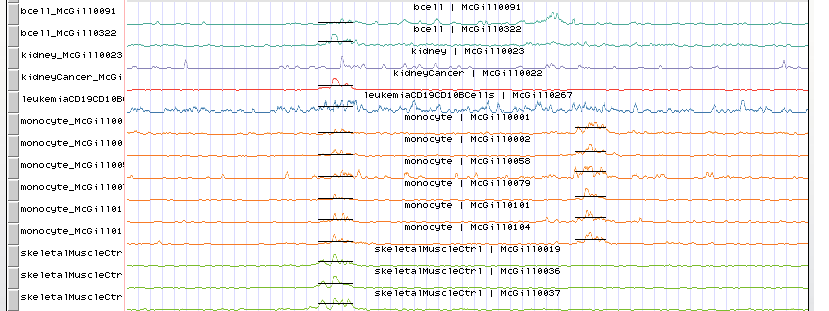
\includegraphics[width=\textwidth]{PeakSegJoint-monocytes-up}
\end{frame}

\section{Other projects and future work}

\begin{frame}
  \frametitle{My research projects include statistical machine
    learning algorithms and biomedical applications}
  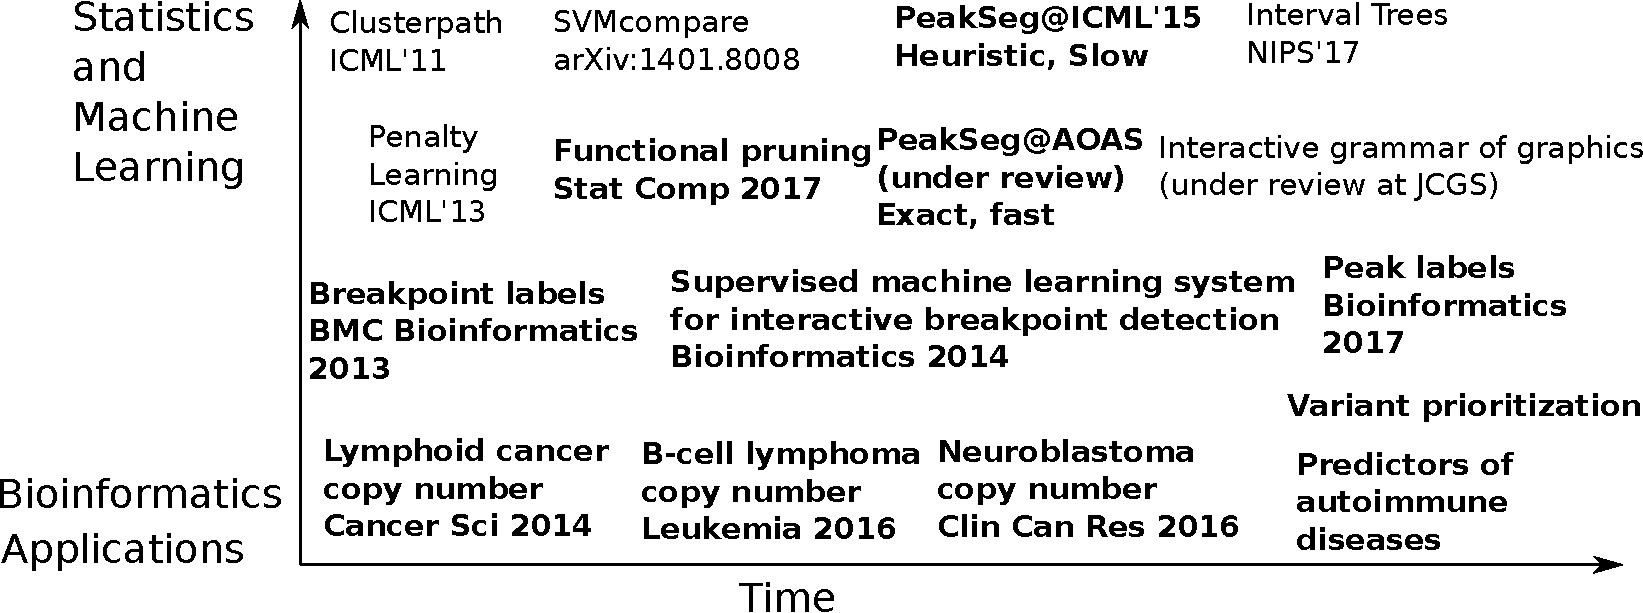
\includegraphics[width=\textwidth]{timeline-SteJustine}
\end{frame}

\begin{frame}
  \frametitle{Other research projects}
  \begin{tabular}{ll}
Clusterpath for convex & \multirow{4}{*}{
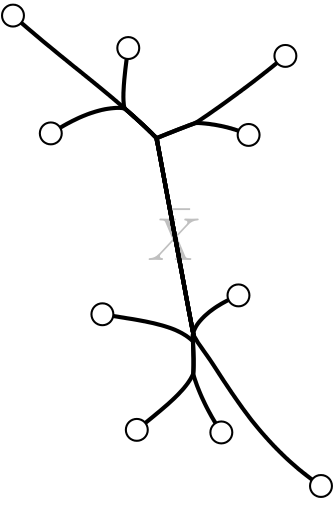
\includegraphics[height=0.2\textheight]{screenshot-clusterpath}
}\\
hierarchical clustering.\\
H {\it et al.}, {\it ICML} 2011\\
91 citations. R package clusterpath. \\
\hline
Support vector machines & \multirow{4}{*}{
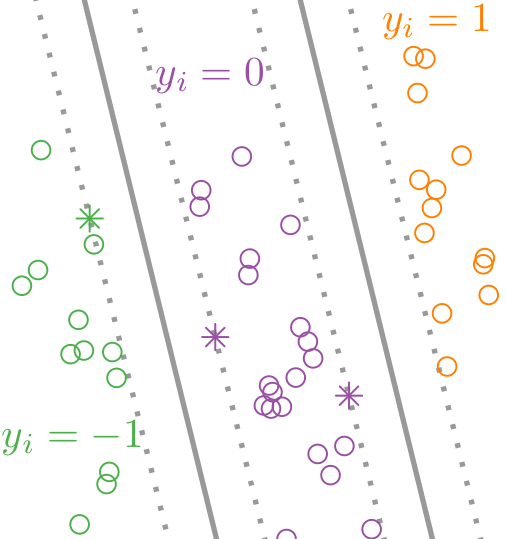
\includegraphics[height=0.2\textheight]{screenshot-ranksvmcompare}
}\\
for ranking and comparison.\\
H {\it et al.}, arXiv:1401.8008. \\
R package rankSVMcompare.\\
\hline
New interactive keywords& \multirow{5}{*}{
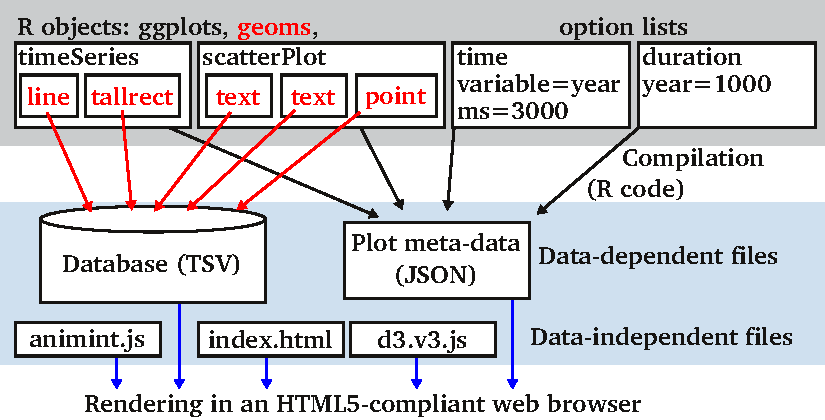
\includegraphics[height=0.2\textheight]{figure-design}
}\\
for the grammar of graphics,\\
under review at \emph{Journal}\\
\emph{ of Computational and Graphical}\\
\emph{Statistics}, R package animint.
  \end{tabular}
  % \begin{minipage}{0.3\linewidth}
  %   Clusterpath for convex hierarchical clustering (H {\it et
  %     al.}, {\it ICML} 2011, 91 citations). R package clusterpath.
  %   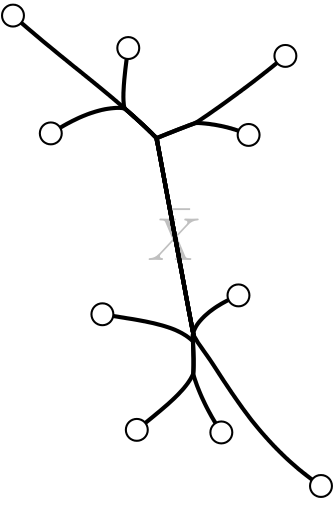
\includegraphics[width=\linewidth]{screenshot-clusterpath}
  % \end{minipage}
  % \begin{minipage}{0.3\linewidth}
  %   Support vector machines for ranking and comparison. H {\it et
  %     al.}, arXiv:1401.8008. R package rankSVMcompare.
  %   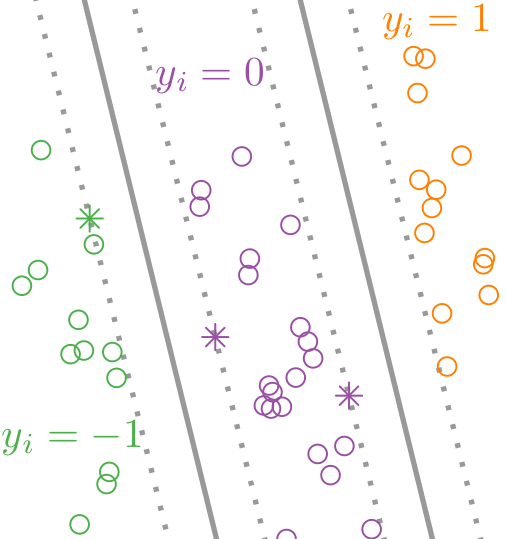
\includegraphics[width=\linewidth]{screenshot-ranksvmcompare}
  % \end{minipage}
  % \begin{minipage}{0.3\linewidth}
  %   New interactive keywords for the grammar of graphics, under review
  %   at \emph{Journal of Computational and Graphical Statistics}, R
  %   package animint.
  % \end{minipage}

  % Collaborations at the McGill Genome Center:
  % \begin{itemize}
  % \item Predicting which people will respond to the flu vaccine based
  %   on SNP data. (with Maiko Narahara)
  % \item Predicting which people have asthma based on SNP
  %   data. (with Audrey Grant)
  % \item Predicting which genetic variants are pathogenic based on
  %   biochemistry, evolutionary conservation, etc. (with
  %   Najmeh Alirezaie)
  % % \item Predicting genomic regions with peaks based on ChIP-seq
  % %   data. (with Guillaume Bourque)
  % \end{itemize}
\end{frame}

\begin{frame}
  \frametitle{Future projects for my research lab}
  \begin{itemize}
  \item More collaborations with biomedical scientists.
  \item Survival models for predicting the number of changepoints: R
    package iregnet.
  \item Functional pruning algorithms for other constrained
    changepoint models (neuro spike train data).
  \item Multi-task learning for predicting the number of changepoints
    (multiple scientists provide breakpoint or peak labels).
  \item Deep learning for nonparametric changepoint detection.
  \item GenomicLearner platform for collaborations: interactive
    labeling and machine learning analysis.
  \end{itemize}
\end{frame}

\begin{frame}
  \frametitle{Previous work limited to 
    unsupervised methods
which are neither interactive nor accurate
}
  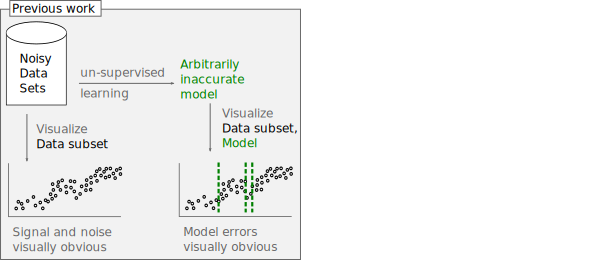
\includegraphics[height=0.5\textheight]{GenomicLearner-unsupervised.pdf}
\end{frame}

\begin{frame}
  \frametitle{GenomicLearner, an public web app for supervised interactive machine learning in genomic data}
  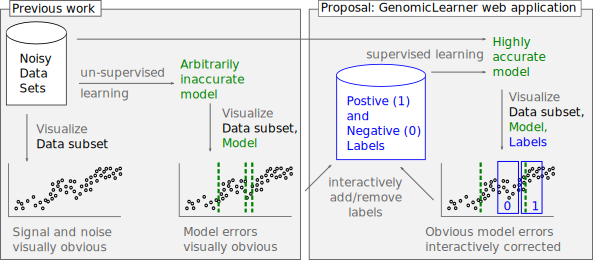
\includegraphics[height=0.5\textheight]{GenomicLearner-both.pdf}
\end{frame}


\begin{frame}
  \frametitle{Thanks for your attention!}

Any questions?

\hskip 1cm

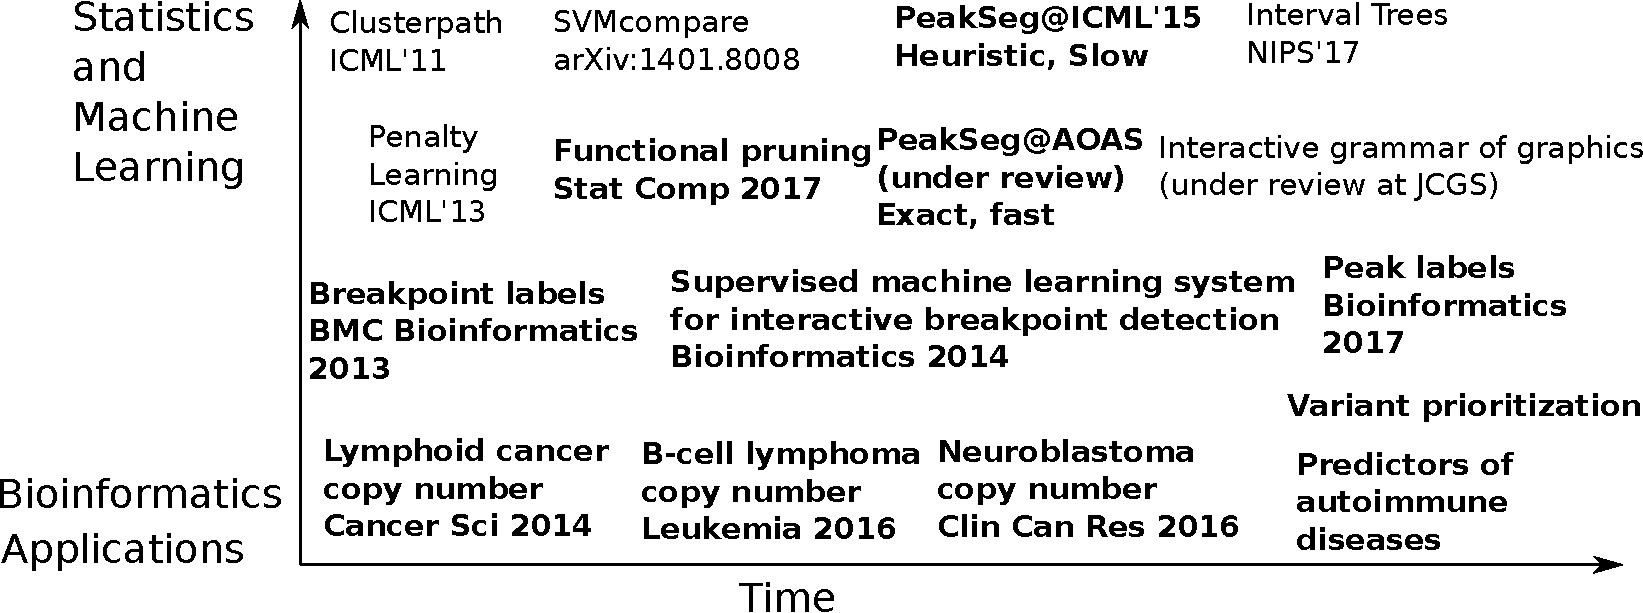
\includegraphics[width=\textwidth]{timeline-SteJustine}

  % Write me at \alert{\texttt{toby.hocking@mail.mcgill.ca}} to collaborate!

  % \vskip 1cm

  % timeline?

\end{frame}

\begin{frame}
  \frametitle{Future work}
  \begin{itemize}
  \item More collaborations with biomedical scientists.
  \item Survival models for penalty function learning: R package
    iregnet.
  \item Multi-task penalty function learning: how to 
  \item Functional pruning algorithms for other constrained
    changepoint models.
  \item GenomicLearner platform for interactive analysis and
    collboarations.
  \item Deep learning for nonparametric changepoint detection.
  \end{itemize}
\end{frame}

\begin{frame}
  \frametitle{Test error in three different experiments}
  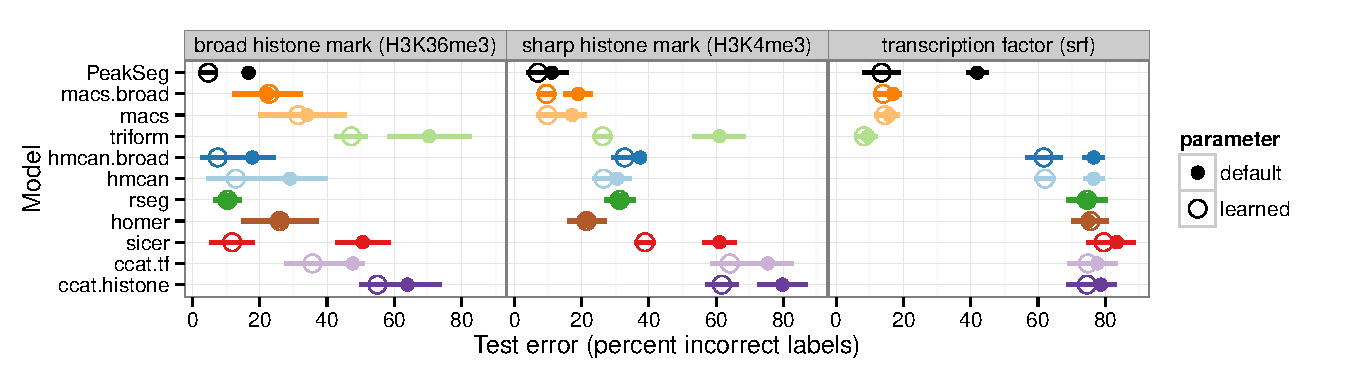
\includegraphics[width=1.1\textwidth]{figure-test-error-dots-mean.pdf}
\end{frame}

\begin{frame}
  \frametitle{Accuracy benchmark: 10 manually labeled data sets}
  \url{http://cbio.ensmp.fr/~thocking/chip-seq-chunk-db/}
  \begin{itemize}
  \item We created 12,826 labels in 7 new data sets.
  \item 4 annotators (AM, TDH, PGP, XJ).
  \item 8 cell types.
  \item 37 H3K4me3 samples (sharp peak pattern).
  \item 29 H3K36me3 samples (broad peak pattern).
  \end{itemize}
  \vskip 1cm
  \url{http://tare.medisin.ntnu.no/chipseqbenchmark/}
  \begin{itemize}
  \item 3 data sets from another group's work in 2011.
  \item 3 transcription factors: SRF, NRSF, MAX.
  \item 2 replicates per transcription factor.
  \item Different protocol: label after peak calling.
  \end{itemize}
\end{frame}

\begin{frame}
  \frametitle{Train on some samples, test on others\\
(same histone mark and person)}
  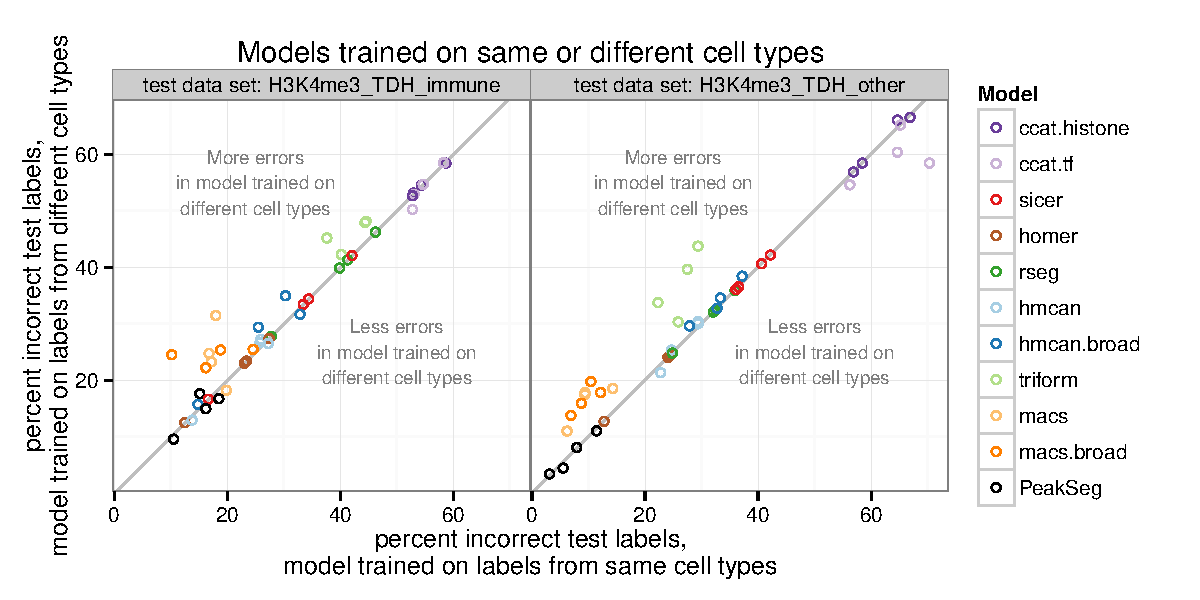
\includegraphics[width=1.1\textwidth]{figure-test-H3K4me3-types.pdf}
\end{frame}

\begin{frame}
  \frametitle{Train on one histone mark, test on another\\
(same person and samples)}
  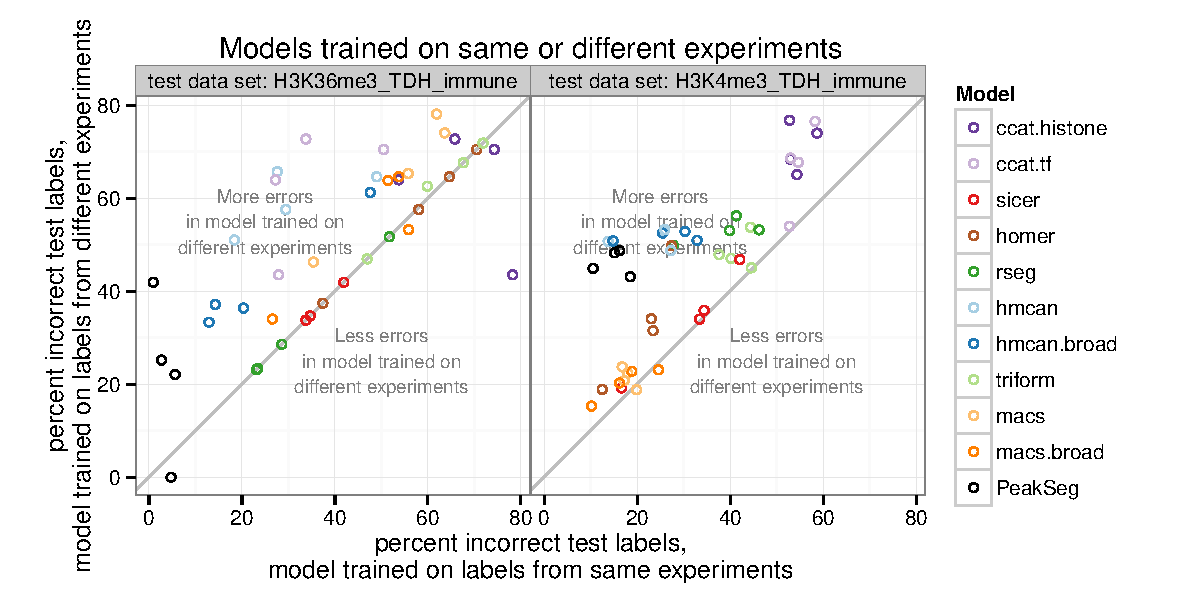
\includegraphics[width=1.1\textwidth]{figure-test-TDH-experiments.pdf}
\end{frame}

\begin{frame}
  \frametitle{Unsupervised algorithms inaccurate for 
    complex patterns}
  \begin{itemize}
  \item Domain expert (e.g. biologist) with prior knowledge manually codes an
    algorithm that recognizes the pattern.
  \item ``if the image $x$ has a dividing cell then predict
    $f(x)=\text{yes}$.''\\
    -- how to code that?
  \item ``if the copy number profile $x$ has a significant change of
    at least p-value $P$ in bins of size $B$, then predict
    $f(x)=\text{breakpoint}$.''\\
    -- sub-optimal parameter choices are inevitable.
    \end{itemize}
Disadvantages:
\begin{itemize}
  \item Need to find someone with programming experience AND domain expertise!
  \item Inaccurate: hard/impossible to manually write code that
    accurately recognizes complex patterns.
  \item Need to write a different algorithm for each pattern (0, 1, 2,
    %shoe, pants, 
    dividing cell, 
    normal cell,
    etc).
  \end{itemize}
\end{frame}

\section*{Learning a penalty function in maximum likelihood changepoint models}

\begin{frame}
  \frametitle{Supervised learning algorithm for breakpoint detection}
  H {\it et al.}, {\it ICML} 2013.
  \begin{itemize}
  \item New method for learning multi-feature linear penalty
    functions in maximum likehood changepoint models.
  \item Previous work: AIC/BIC/mBIC/etc (0 learned parameters)
    and scalar penalties (1 learned parameter).
  \item Contribution: convex optimization problem and learning
    algorithm for regression with censored outputs
    $(\underline L_i, \overline L_i)$.
  \item Results: improves breakpoint detection accuracy (cross-validation experiments).
  \end{itemize}
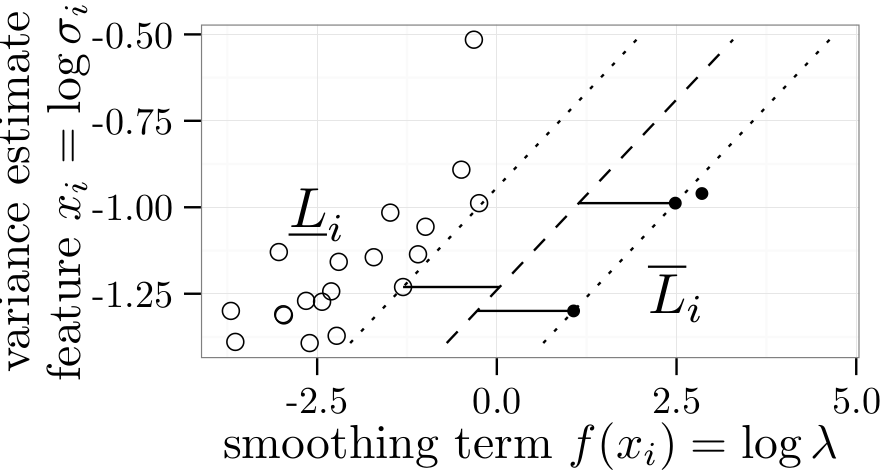
\includegraphics[width=0.4\textwidth]{screenshot-mmir-crop}
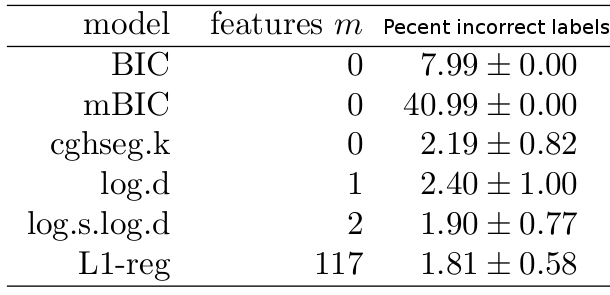
\includegraphics[width=0.4\textwidth]{screenshot-mmir-test-error}
\end{frame}

\begin{frame}
  \frametitle{useR2017 tutorial}
  
\end{frame}

\begin{frame}
  \frametitle{Nonlinear decision tree model}
  Drouin, Hocking, Laviolette {\it NIPS} 2017.
  \begin{itemize}
  \item Contribution: dynamic programming algorithm for learning a
    nonlinear decision tree model.
  \item Results: learns nonlinear patterns, improved
    breakpoint detection accuracy.
  \end{itemize}
%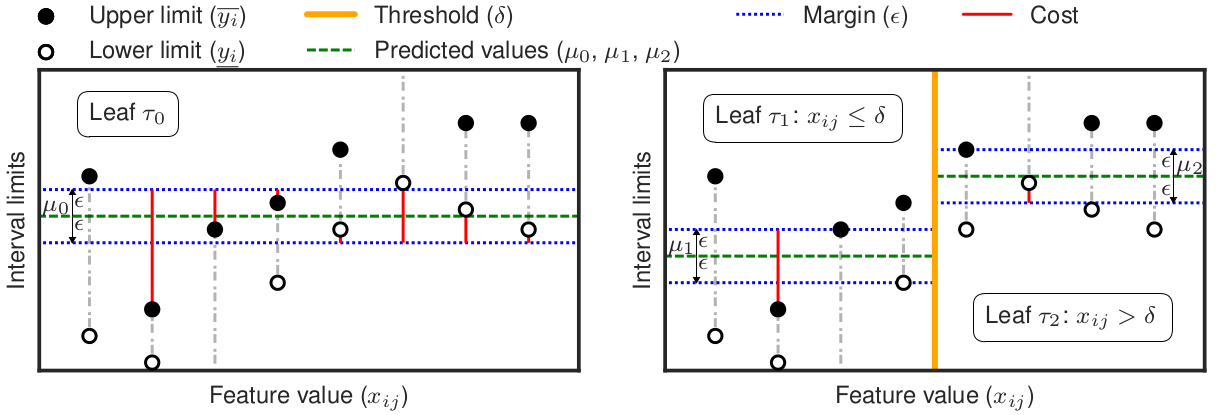
\includegraphics[width=\textwidth]{screenshot-mmit}

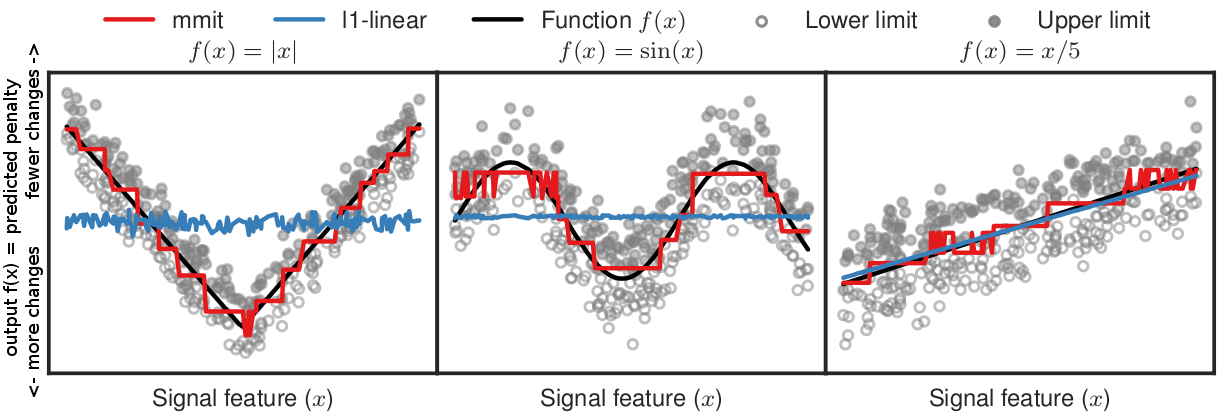
\includegraphics[width=\textwidth]{screenshot-mmit-learned}
\end{frame}

\begin{frame}
  \frametitle{Maximum Gaussian likelihood changepoint detection}

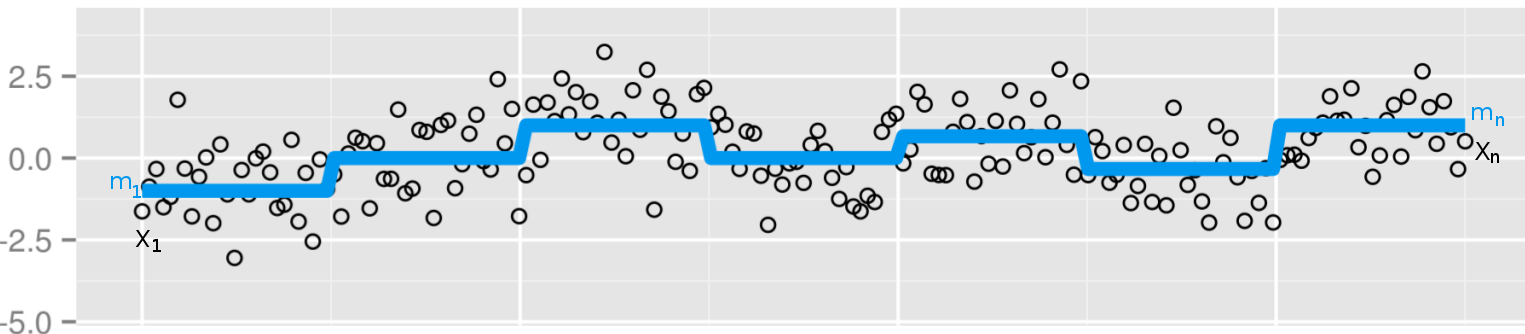
\includegraphics[width=\textwidth]{seg-mean}
\begin{align*}
    \minimize_{
  \mathbf m\in\RR^{n}
} &\ \ 
    \underbrace{
    \sum_{i=1}^n ( m_i - x_i)^2
}_{\text{fit the data}} + 
\underbrace{\lambda
\sum_{i=1}^{n-1} I(m_i\neq m_{i+1})}_{
\text{penalize number of changes}
}
\end{align*}

\begin{itemize}
\item Optimization variable $\mathbf m$ is the segment mean.
\item Minimizing the square loss corresponds to maximizing the
  Gaussian likelihood.
\item Penalty term encourages a model with few changes.
\item Penalty $\lambda=0$ means a change after every data point.
\item Penalty $\lambda=\infty$ means no changes.
\end{itemize}
\end{frame}

\end{document}

 